\documentclass[11pt,a4paper]{report}

\usepackage[T1]{fontenc}
\usepackage[utf8]{inputenc}
\usepackage[margin=1in,headheight=14pt]{geometry}
\usepackage{graphicx}
\usepackage{textcomp}
% Load order matters: pandoc sizes table columns with \real{...}, which the
% array package provides.  calc claims \real for itself if it is loaded
% first, and the width arithmetic then fails, so array must come before it.
\usepackage{longtable,booktabs,array}
\usepackage{calc}
\usepackage{xcolor}
\usepackage{listings}
\usepackage{tcolorbox}
\usepackage{etoolbox}
\usepackage{fancyhdr}
\usepackage{hyperref}

\hypersetup{
  colorlinks=true,
  linkcolor=black,
  urlcolor=blue!60!black,
  pdftitle={Complete CCNA 200-301 Course Notes},
}

% --- Images ---------------------------------------------------------------
% Every diagram is scaled to the text block: at most the full line width and
% at most most of the page height, whichever binds first.
\setkeys{Gin}{width=\linewidth,height=0.82\textheight,keepaspectratio}

% --- Tables ---------------------------------------------------------------
% The subnetting charts carry 8-9 columns and do not fit at body text size.
\AtBeginEnvironment{longtable}{\footnotesize}
\setlength{\LTpre}{0.6em}
\setlength{\LTpost}{0.6em}

% --- Code blocks ----------------------------------------------------------
% Some fenced blocks in the notes hold long prose lines.  Plain verbatim
% cannot wrap them and they run off the page, so pandoc is invoked with
% --syntax-highlighting=idiomatic (which emits lstlisting) and listings is
% told to break lines.  The arrow marks a line that was wrapped, so it is
% not mistaken for a new command.
\lstset{
  basicstyle=\ttfamily\small,
  breaklines=true,
  breakautoindent=false,
  columns=fullflexible,
  keepspaces=true,
  frame=none,
  postbreak=\mbox{\textcolor{gray}{$\hookrightarrow$}\space},
  % Code blocks hold curly quotes and ellipses, which listings cannot set
  % on its own.  Markdown also reads 4-space indented text as an indented
  % code block, so this has to cover content the preprocessing pass in
  % build_chapters.py never sees.
  extendedchars=true,
  inputencoding=utf8,
  literate={‘}{{'}}1 {’}{{'}}1 {“}{{"}}1 {”}{{"}}1
           {…}{...}3 {→}{{$\rightarrow$}}1 {–}{{-}}1 {—}{{--}}1
           {💡}{{Tip:}}4 {🚨}{{!}}1,
}

% --- List nesting ---------------------------------------------------------
% LaTeX's itemize and enumerate stop at four levels; the DHCP snooping notes
% go one deeper and abort the run with "Too deeply nested".  Raise the two
% thresholds and supply the label the extra level needs.
\makeatletter
\patchcmd{\itemize}{\@itemdepth >\thr@@}{\@itemdepth >5\relax}{}%
  {\@latex@warning{CCNA: could not raise the itemize nesting depth}}
\patchcmd{\enumerate}{\@enumdepth >\thr@@}{\@enumdepth >5\relax}{}%
  {\@latex@warning{CCNA: could not raise the enumerate nesting depth}}
\makeatother
\newcommand{\labelitemv}{\textbullet}

% --- Pandoc compatibility -------------------------------------------------
% pandoc emits these in its LaTeX output; they are normally supplied by its
% own template, which we are not using.
\providecommand{\tightlist}{%
  \setlength{\itemsep}{0pt}\setlength{\parskip}{0pt}}
\providecommand{\pandocbounded}[1]{#1}
% Wraps inline code when a highlighting style is active.
\providecommand{\passthrough}[1]{#1}
% pandoc wraps uncaptioned tables in \def\LTcaptype{none}; the counter it
% refers to is defined by pandoc's own template.
\newcounter{none}
% Gives TeX more room to stretch a line before it gives up and overflows.
\setlength{\emergencystretch}{3em}

% --- Callout boxes --------------------------------------------------------
\tcbuselibrary{breakable}
\newtcolorbox{tipbox}{
  breakable, colback=blue!5, colframe=blue!55!black,
  boxrule=0.4pt, arc=2pt, left=6pt, right=6pt, top=6pt, bottom=6pt,
  title=Tip, fonttitle=\bfseries\small, coltitle=white,
  colbacktitle=blue!55!black, before skip=8pt, after skip=8pt,
}
\newtcolorbox{warnbox}{
  breakable, colback=orange!8, colframe=orange!80!black,
  boxrule=0.4pt, arc=2pt, left=6pt, right=6pt, top=6pt, bottom=6pt,
  title=Warning, fonttitle=\bfseries\small, coltitle=white,
  colbacktitle=orange!80!black, before skip=8pt, after skip=8pt,
}

% --- Page style -----------------------------------------------------------
\pagestyle{fancy}
\fancyhf{}
\fancyhead[L]{\nouppercase{\leftmark}}
\fancyhead[R]{\thepage}
\renewcommand{\headrulewidth}{0.4pt}
\fancypagestyle{plain}{\fancyhf{}\fancyhead[R]{\thepage}%
  \renewcommand{\headrulewidth}{0pt}}

% Chapters and sections in the contents; the notes' topic lines become
% sections, so this is what makes the report navigable.
\setcounter{tocdepth}{1}

% ---------------------------------------------------------------------------
\begin{document}

\begin{titlepage}
  \centering
  \vspace*{3cm}
  {\Huge\bfseries Complete CCNA 200-301\\[0.4em] Course Notes\par}
  \vspace{1.5cm}
  {\large A single reference assembled from 66 chapters of\\[0.3em]
   personal course notes\par}
  \vfill
  {\large Notes taken during Jeremy's IT Lab\\[0.2em]
   \emph{Complete Course for the CCNA 200-301}\par}
  \vspace{1.2cm}
  {\small Based on the note collection at\\
   \url{https://github.com/psaumur/CCNA_Course_Notes}\par}
  \vspace{2cm}
  {\small\today\par}
\end{titlepage}

\tableofcontents

\chapter{Networking Devices}\label{networking-devices}

\section{What is a network?}\label{what-is-a-network}

A computer network is a digital telecommunications network allows NODES
to share RESOURCES.

A CLIENT is a device that accesses a service made available by a SERVER.

A SERVER is a device that provides functions or services for CLIENTS.

\begin{itemize}
\tightlist
\item
  Note : The same device can be a CLIENT in some situations and a SERVER
  in other situations. Ex: A Peer-to-Peer network.
\end{itemize}

SWITCHES (Level 2):

\begin{itemize}
\tightlist
\item
  provide connectivity to hosts within the same LAN (Local Area Network)
\item
  Have many network interfaces/ports for End Hosts to connect to.
\item
  DO NOT provide connectivity between LANs/over the Internet.
\end{itemize}

ROUTERS (Level 3):

\begin{itemize}
\tightlist
\item
  have fewer network interfaces than switches.
\item
  are used to provide connectivity BETWEEN LANs.
\item
  are used to send data over the Internet.
\end{itemize}

FIREWALL (Can be Level 3,4, and 7):

\begin{itemize}
\tightlist
\item
  Firewalls are specialty hardware network security devices that control
  network traffic entering/exiting your network.
\item
  Can be places ``inside'' or ``outside'' the network.
\item
  Monitor and control network traffic based on configured rules.
\item
  Are known as ``Next-Generation Firewalls'' when they include more
  modern and advanced filtering capabilities.
\item
  Host-based firewalls are software applications that filter traffic
  entering and exiting a host machine, like a PC.
\end{itemize}

\chapter{Interfaces and Cables}\label{interfaces-and-cables}

SWITCHES provide many PORTS for connectivity (usually 24)

These PORTS tend to be RJ-45 (Registered Jack) ports.

WHAT IS ETHERNET?

\begin{itemize}
\tightlist
\item
  Ethernet is a collection of network protocols/standards.
\end{itemize}

Why do we need network protocols and standards?

\begin{itemize}
\tightlist
\item
  provide common communication standards over networks.
\item
  provide common hardware standards to allow connectivity between
  devices.
\end{itemize}

Connections between devices operates at a set speed.

These speeds are measured in ``bits per second'' (bps)

A bit is a value of ``0'' or ``1''. A byte is 8 bits (0s and 1s)

{\def\LTcaptype{none} % do not increment counter
\begin{longtable}[]{@{}ll@{}}
\toprule\noalign{}
Size & \# of Bits \\
\midrule\noalign{}
\endhead
\bottomrule\noalign{}
\endlastfoot
1 kilobit (Kb) & 1,000 \\
1 megabit (Mb) & 1,000,000 \\
1 gigabit (Gb) & 1,000,000,000 \\
1 terabit (Tb) & 1,000,000,000,000 \\
\end{longtable}
}

Ethernet standards are:

\begin{itemize}
\tightlist
\item
  Defined in the IEEE 802.3 standard in 1983
\item
  IEEE = Institute of Electrical and Electronics Engineers
\end{itemize}

\section{Ethernet Standards (Copper)}\label{ethernet-standards-copper}

{\def\LTcaptype{none} % do not increment counter
\begin{longtable}[]{@{}
  >{\raggedright\arraybackslash}p{(\linewidth - 8\tabcolsep) * \real{0.2000}}
  >{\raggedright\arraybackslash}p{(\linewidth - 8\tabcolsep) * \real{0.2000}}
  >{\raggedright\arraybackslash}p{(\linewidth - 8\tabcolsep) * \real{0.2000}}
  >{\raggedright\arraybackslash}p{(\linewidth - 8\tabcolsep) * \real{0.2000}}
  >{\raggedright\arraybackslash}p{(\linewidth - 8\tabcolsep) * \real{0.2000}}@{}}
\toprule\noalign{}
\begin{minipage}[b]{\linewidth}\raggedright
Speed
\end{minipage} & \begin{minipage}[b]{\linewidth}\raggedright
Common Name
\end{minipage} & \begin{minipage}[b]{\linewidth}\raggedright
Standard
\end{minipage} & \begin{minipage}[b]{\linewidth}\raggedright
Cable Type
\end{minipage} & \begin{minipage}[b]{\linewidth}\raggedright
Max Transmission Distance
\end{minipage} \\
\midrule\noalign{}
\endhead
\bottomrule\noalign{}
\endlastfoot
10 Mbps & Ethernet & 802.3i & 10BASE-T & 100m Max \\
100 Mbps & Fast Ethernet & 802.3u & 100BASE-T & 100m Max \\
1 Gbps & Gigabit Ethernet & 802.3ab & 1000BASE-T & 100m Max \\
10 Gbps & 10 Gigabit Ethernet & 802.3an & 10GBASE-T & 100m Max \\
\end{longtable}
}

BASE = refers to Baseband Signaling

T = Twisted Pair

Most Ethernet uses copper cables.

UTP or Unshielded Twisted Pair (no metallic shield) Twist protects
against EMI (Electromagnetic Interference)

Most use 8 wires (4 pairs) however \ldots{}

10/100BASE-T = 2 pairs (4 wires)

\begin{figure}
\centering
\pandocbounded{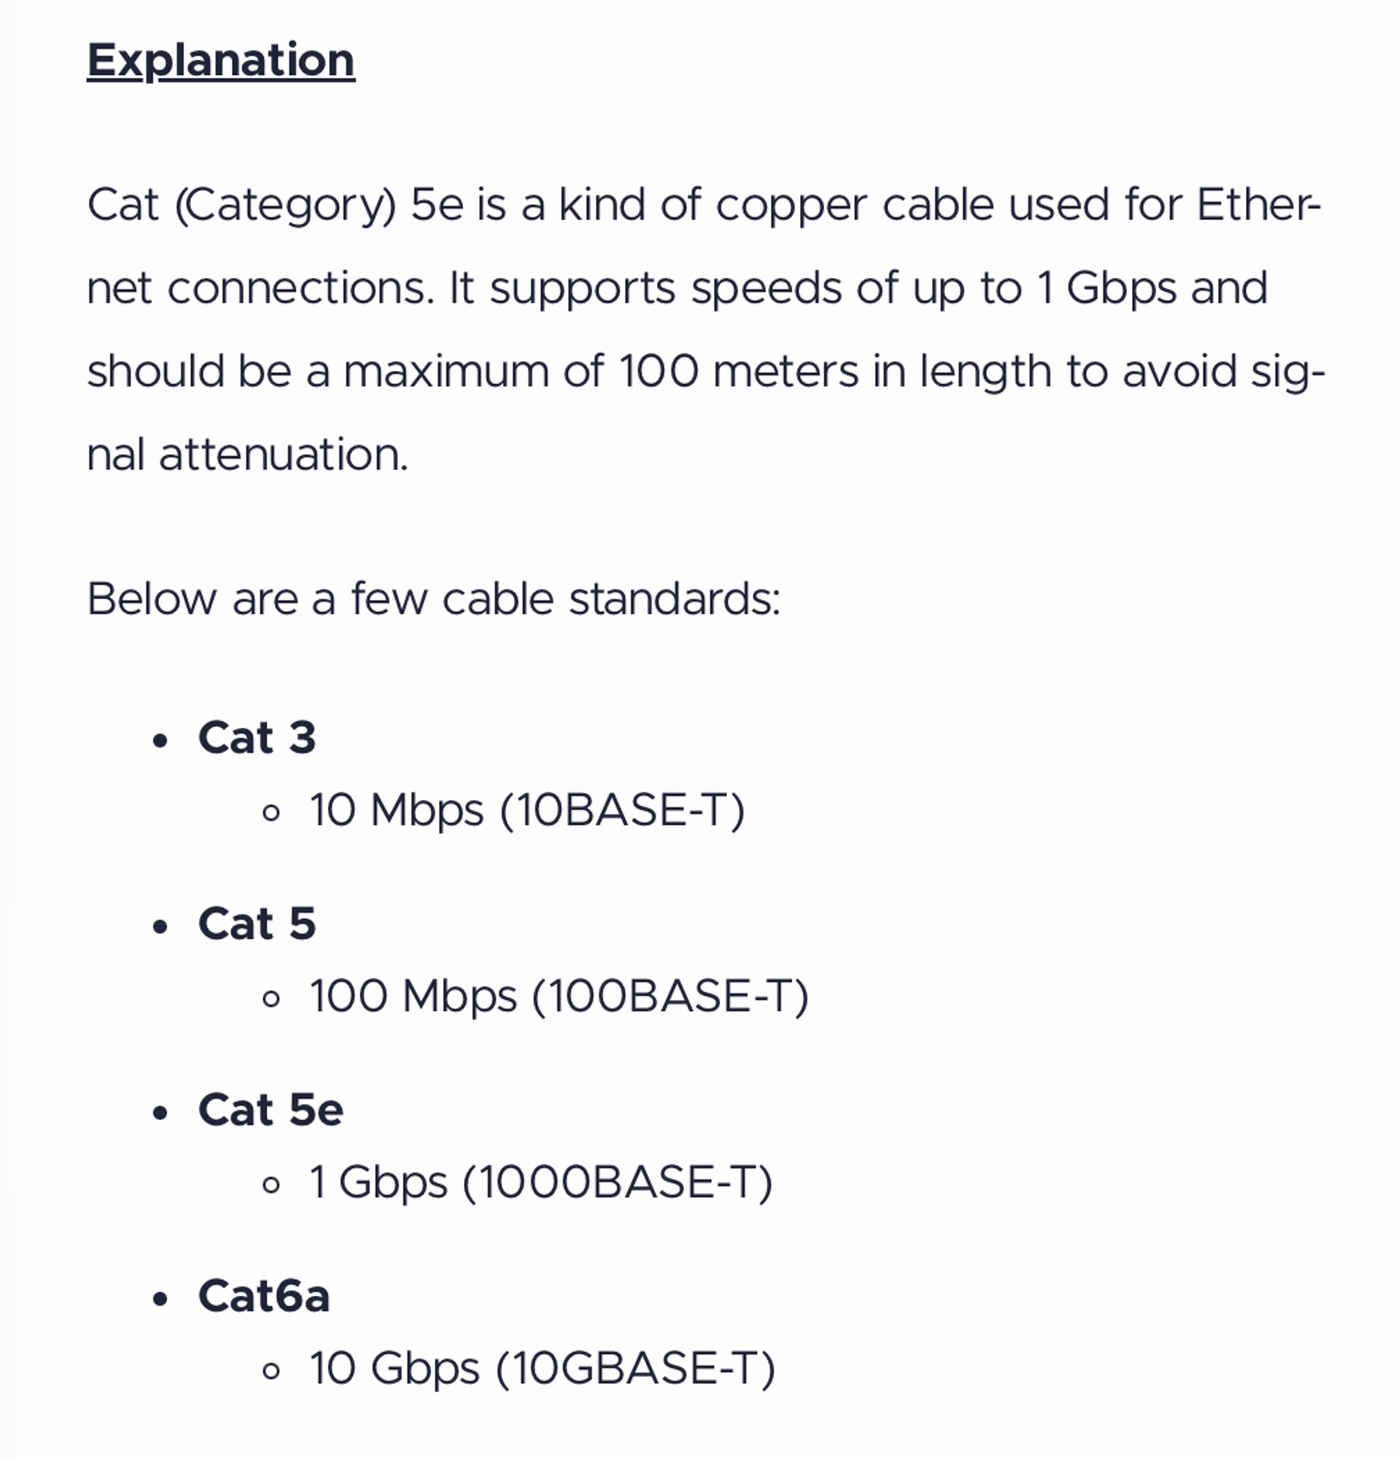
\includegraphics[keepaspectratio,alt={image}]{images/02-interfaces-and-cables/img-001.png}}
\end{figure}

How do devices communicate via their connections?

Each ethernet cable has a RJ-45 plug with 8 pins on the ends.

\begin{figure}
\centering
\pandocbounded{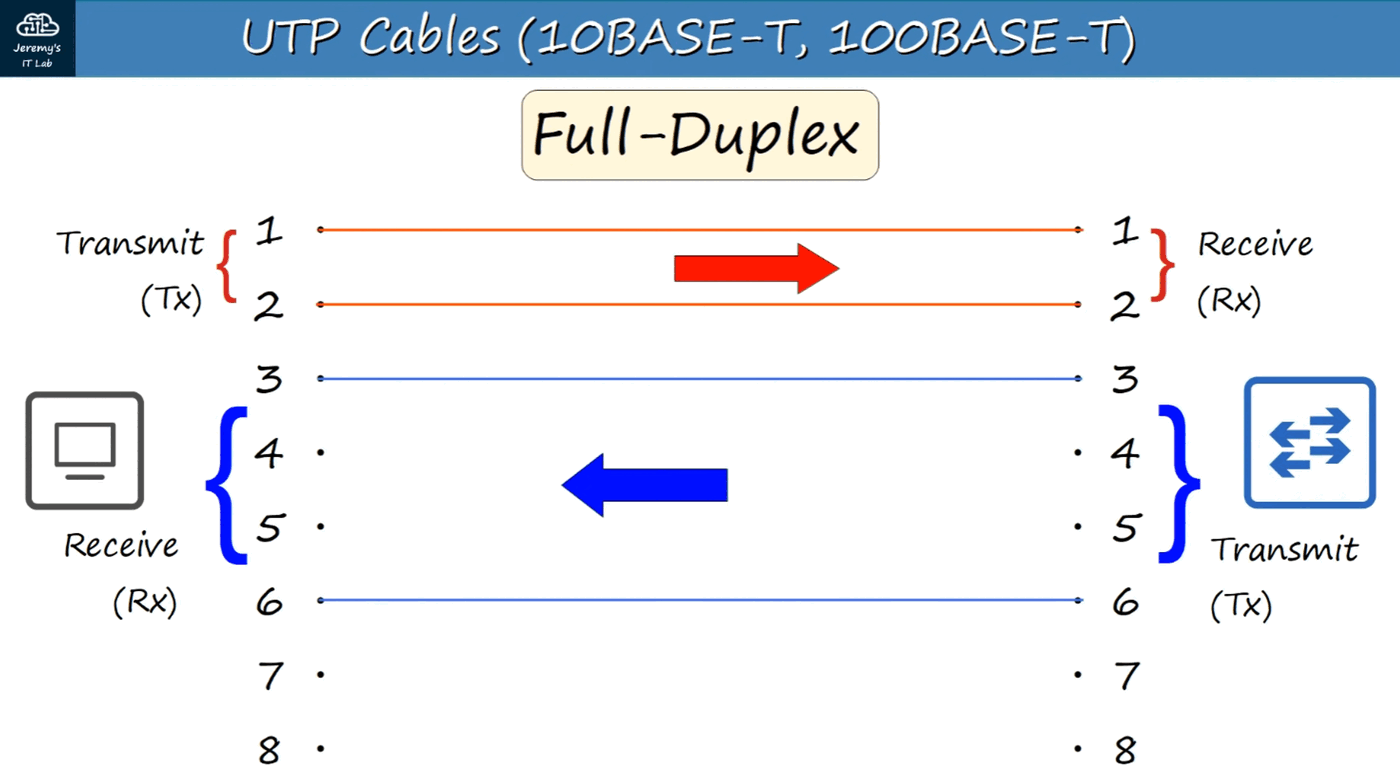
\includegraphics[keepaspectratio,alt={image}]{images/02-interfaces-and-cables/img-002.png}}
\end{figure}

\begin{itemize}
\tightlist
\item
  PCs Transmit(TX) data on Pins \#1-2
\item
  Switches Receive(RX) data on Pins \#1-2
\item
  PCs Receive(RC) data on Pins \#3,6
\item
  Switches Transmit(TX) data on Pins \#3,6
\end{itemize}

This allows Full-Duplex transmission of data.

What if a Router / Switch connect?

\begin{figure}
\centering
\pandocbounded{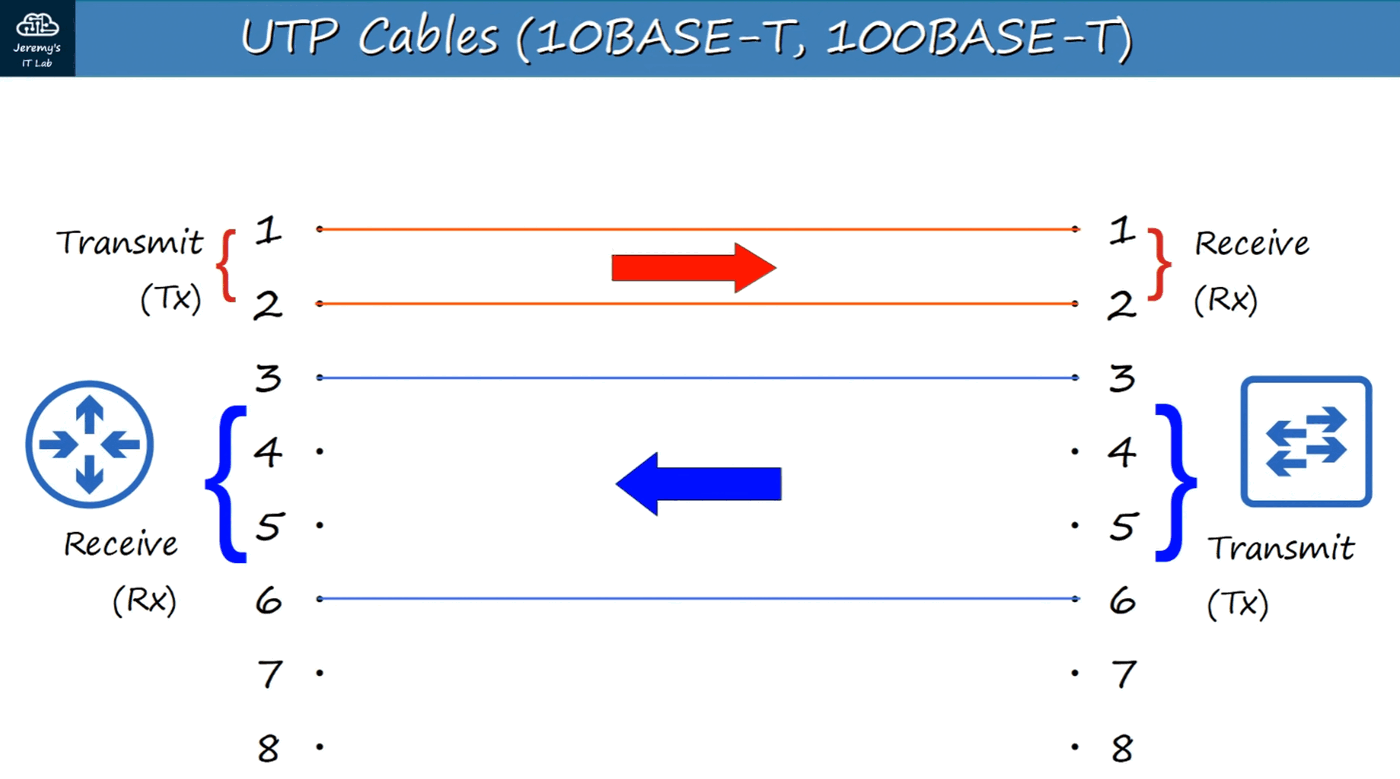
\includegraphics[keepaspectratio,alt={image}]{images/02-interfaces-and-cables/img-003.png}}
\end{figure}

\begin{itemize}
\tightlist
\item
  Routers Transmit(TX) data on Pins \#1-2
\item
  Routers Receive(RX) data on Pins \#3,6
\item
  Switches Transmit(TX) data on Pins \#3,6
\item
  Switches Receive(RX) data on Pins \#1-2
\end{itemize}

Routers and PCs connect the same way with Switches.

The cable used to connect is called a ``Straight-Through'' cable.

What if we want to connect similar devices to each other?

We CANNOT use a ``Straight-Through'' cable. We MUST use a ``Crossover''
cable.

This cable swaps the pins on one end to allow connection to work.

\begin{figure}
\centering
\pandocbounded{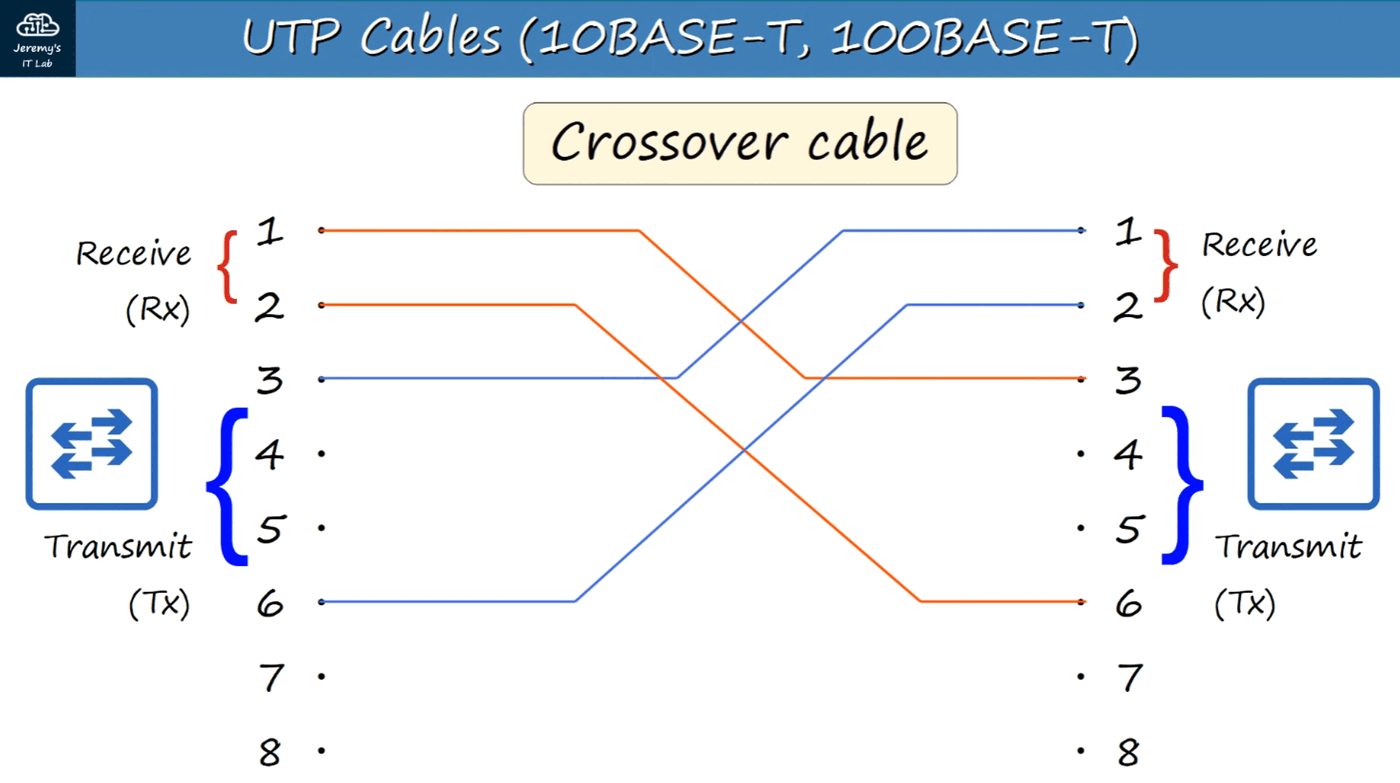
\includegraphics[keepaspectratio,alt={image}]{images/02-interfaces-and-cables/img-004.png}}
\end{figure}

PIN\#1 -----\textgreater{} PIN\#3 PIN\#2 -----\textgreater{} PIN\#6

PIN\#3 -----\textgreater{} PIN\#1 PIN\#6 -----\textgreater{} PIN\#2

{\def\LTcaptype{none} % do not increment counter
\begin{longtable}[]{@{}lll@{}}
\toprule\noalign{}
DEVICE TYPE & TRANSMIT (TX) PINS & RECEIVE (RX) PINS \\
\midrule\noalign{}
\endhead
\bottomrule\noalign{}
\endlastfoot
ROUTER & 1 and 2 & 3 and 6 \\
FIREWALL & 1 and 2 & 3 and 6 \\
PC & 1 and 2 & 3 and 6 \\
SWITCH & 3 and 6 & 1 and 2 \\
\end{longtable}
}

Most modern equipment now has AUTO MDI-X which \textbf{automatically
detects} which pins their neighbour is transmitting on and adjust the
pins they receive data on.

1000BASE-T/10GBASE-T = 4 pairs (8 wires)

Each wire pair is \textbf{bidirectional} so can transmit/receive much
faster than 10/100BASE-T.

\begin{figure}
\centering
\pandocbounded{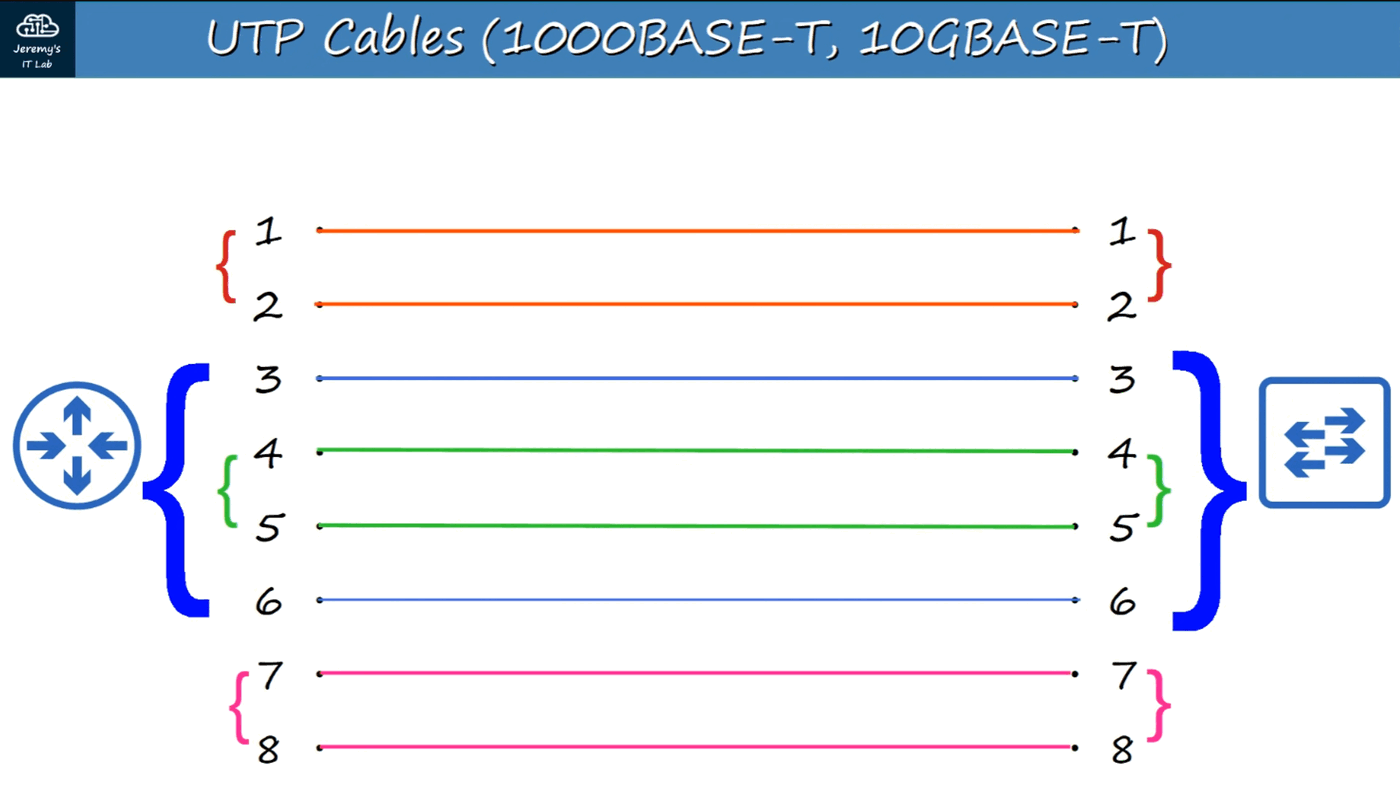
\includegraphics[keepaspectratio,alt={image}]{images/02-interfaces-and-cables/img-005.png}}
\end{figure}

Fiber-Optic Connections:

\begin{itemize}
\tightlist
\item
  Defined in the IEEE 802.3ae standard
\end{itemize}

SFP Transceiver (Small Form-Factor Pluggable) allows fiber-optic cables
to connect to switches/routers.

\begin{itemize}
\tightlist
\item
  Have separate cables to transmit / receive.
\end{itemize}

4 parts to a fiber-optic cable.

\begin{figure}
\centering
\pandocbounded{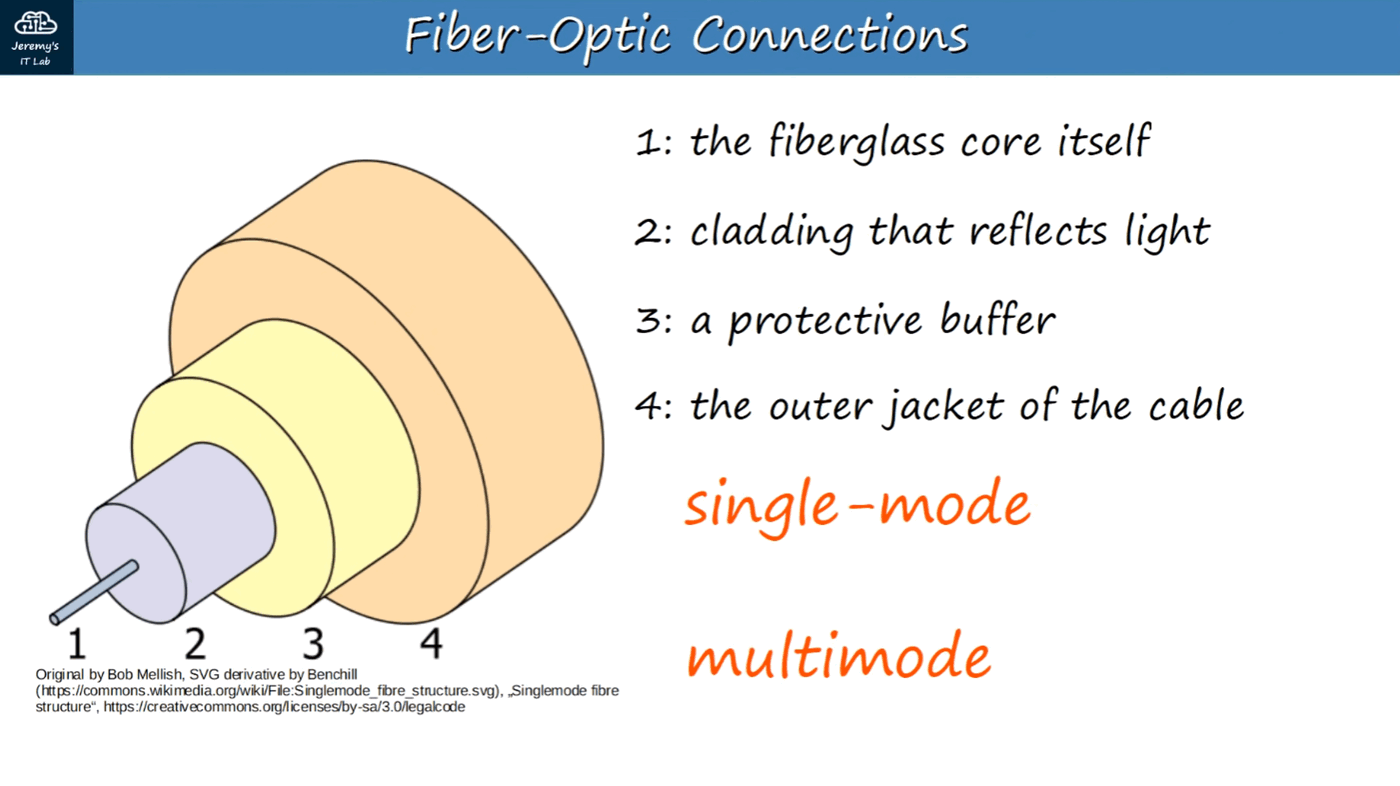
\includegraphics[keepaspectratio,alt={image}]{images/02-interfaces-and-cables/img-006.png}}
\end{figure}

There are TWO types of fiberoptic cable.

Single-Mode:

\begin{figure}
\centering
\pandocbounded{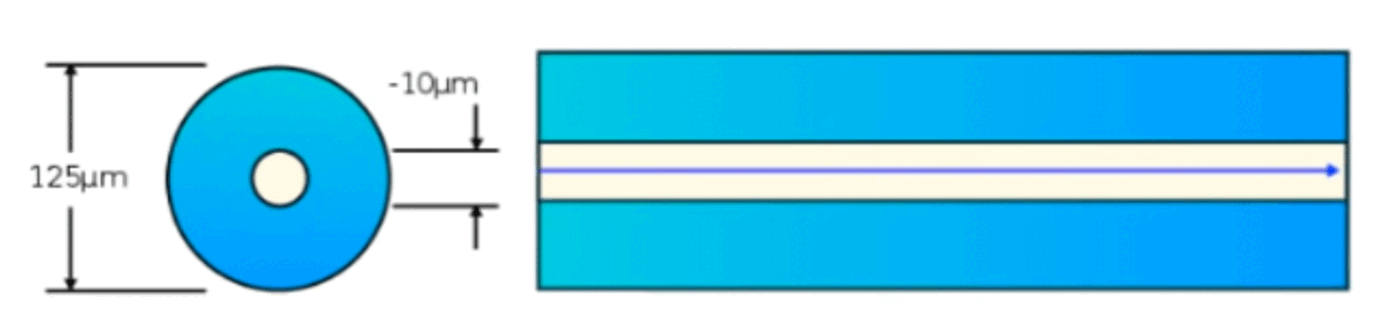
\includegraphics[keepaspectratio,alt={image}]{images/02-interfaces-and-cables/img-007.png}}
\end{figure}

\begin{itemize}
\tightlist
\item
  Narrower than multimode
\item
  Lighter enters at a single angle (mode) from a laser-based
  transmitter.
\item
  Allows longer cables than both UTP and multimode fiber.
\item
  More expensive than multimode fiber (due to more expensive laser-based
  SFP transmitters)
\end{itemize}

Multimode:

\begin{figure}
\centering
\pandocbounded{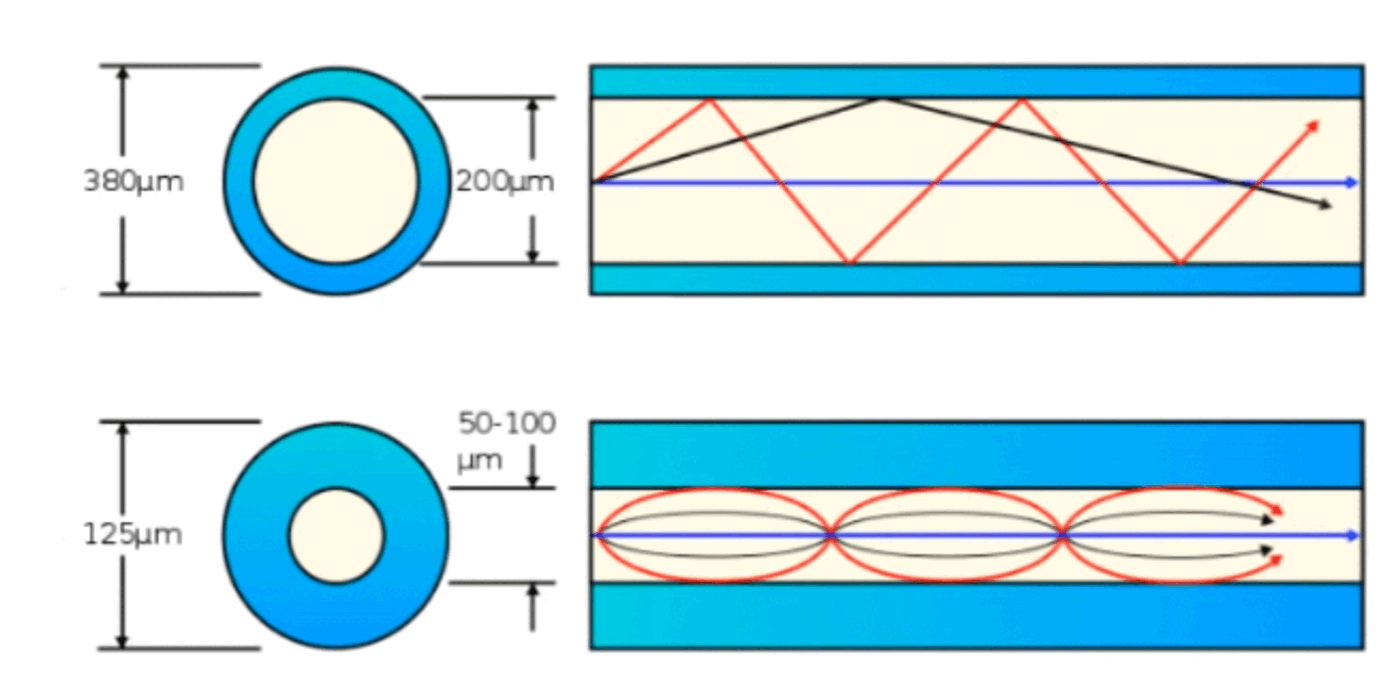
\includegraphics[keepaspectratio,alt={image}]{images/02-interfaces-and-cables/img-008.png}}
\end{figure}

\begin{itemize}
\tightlist
\item
  Core is wider than Single-mode
\item
  Allows multiple angles (modes) of light waves to enter core
\item
  Allows longer cables than UTP but shorter than single-mode
\item
  Cheaper than single-mode fiber (due to cheaper LED-based SFP
  transmitter)
\end{itemize}

Fiber Optic Standards:

{\def\LTcaptype{none} % do not increment counter
\begin{longtable}[]{@{}
  >{\raggedright\arraybackslash}p{(\linewidth - 8\tabcolsep) * \real{0.2000}}
  >{\raggedright\arraybackslash}p{(\linewidth - 8\tabcolsep) * \real{0.2000}}
  >{\raggedright\arraybackslash}p{(\linewidth - 8\tabcolsep) * \real{0.2000}}
  >{\raggedright\arraybackslash}p{(\linewidth - 8\tabcolsep) * \real{0.2000}}
  >{\raggedright\arraybackslash}p{(\linewidth - 8\tabcolsep) * \real{0.2000}}@{}}
\toprule\noalign{}
\begin{minipage}[b]{\linewidth}\raggedright
Speed
\end{minipage} & \begin{minipage}[b]{\linewidth}\raggedright
Standard
\end{minipage} & \begin{minipage}[b]{\linewidth}\raggedright
Connection Speed
\end{minipage} & \begin{minipage}[b]{\linewidth}\raggedright
Mode Support
\end{minipage} & \begin{minipage}[b]{\linewidth}\raggedright
Max Transmission Distance
\end{minipage} \\
\midrule\noalign{}
\endhead
\bottomrule\noalign{}
\endlastfoot
1000BASE-LX & 802.3z & 1 Gbps & Multimode / Single & 550 meters (Multi)
/ 5km (Single) \\
10GBASE-SR & 802.3ae & 10 Gbps & Multimode & 400 meters \\
10GBASE-LR & 802.3ae & 10 Gbps & Single & 10 kilometers \\
10GBASE-ER & 802.3ae & 10 Gbps & Single & 30 kilometers \\
\end{longtable}
}

UTP vs Fiber-Optic Cabling:

UTP are:

\begin{itemize}
\tightlist
\item
  Lower cost than fiber-optic.
\item
  Shorter maximum distance than fiber-optic (\textasciitilde100m).
\item
  Can be vulnerable to EMI (Electromagnetic Interference).
\item
  RJ45 ports used with UTP are cheaper than SFP ports.
\item
  Emit (leak) a faint signal outside of cable, which can be copied
  (security risk).
\end{itemize}

Fiber-Optic:

\begin{itemize}
\tightlist
\item
  Higher cost than UTP.
\item
  Longer maximum distance than UTP.
\item
  No vulnerability to EMI.
\item
  SFP ports are more expensive than RJ45 ports (single-mode is more
  expensive than multimode).
\item
  Does not emit any signal outside of the cable (no security risk).
\end{itemize}

\chapter{The OSI Model and TCP/IP
Suite}\label{the-osi-model-and-tcpip-suite}

\section{What is a networking model?}\label{what-is-a-networking-model}

Networking models categorize and provide a structure for networking
protocols and standards.

(Protocols are a set of logical rules defining how network devices and
software should work)

\section{OSI MODEL}\label{osi-model}

\begin{itemize}
\tightlist
\item
  Open Systems Interconnection Model
\item
  Conceptual model that categorizes and standardizes the different
  functions in a network.
\item
  Created by the ``International Organization for Standardization''
  (ISO)
\item
  Functions are divided into 7 ``Layers''
\item
  These layers work together to make the network work.
\end{itemize}

\begin{figure}
\centering
\pandocbounded{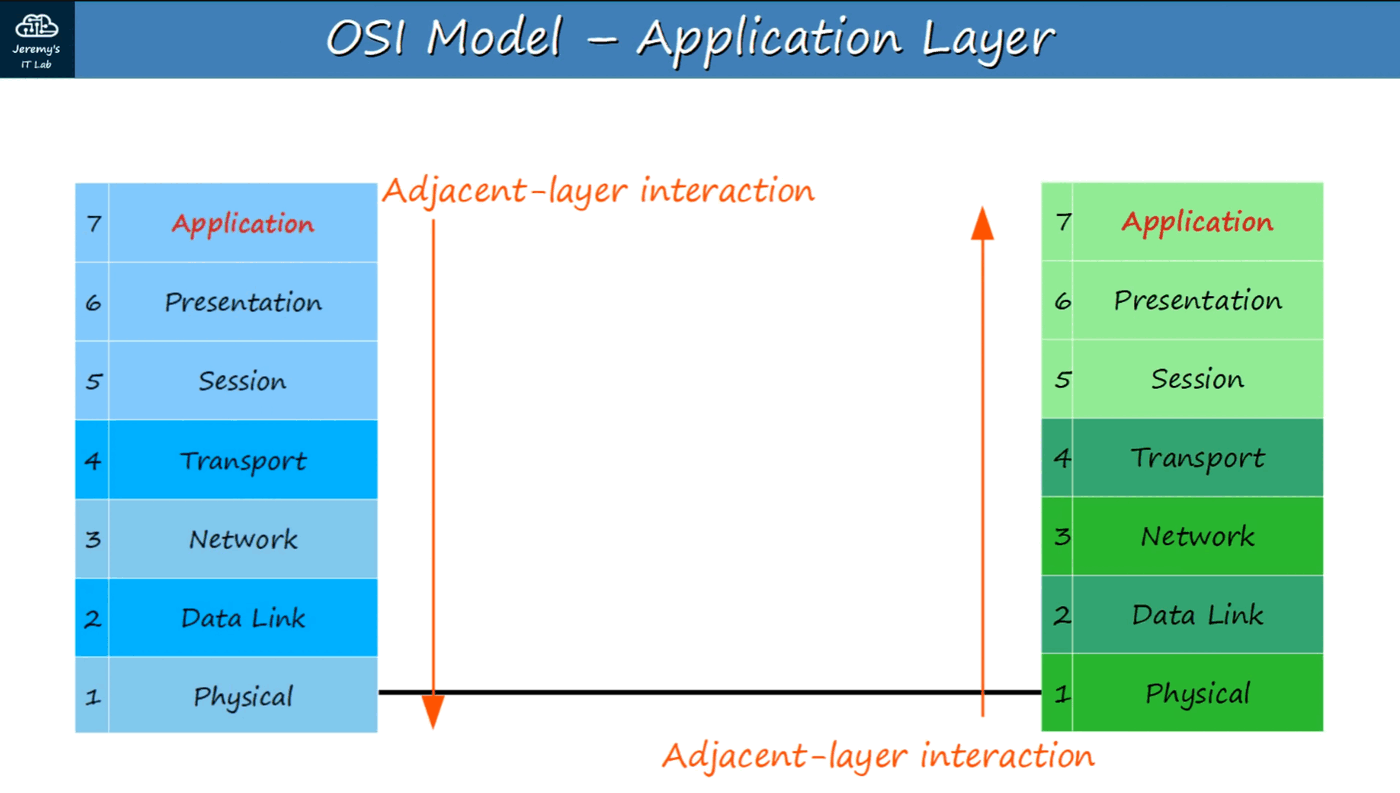
\includegraphics[keepaspectratio,alt={image}]{images/03-osi-model-tcpsuite/img-001.png}}
\end{figure}

As data moves from the top layer, downward, the process is called
``encapsulation''

As data moves from the bottom layer, upward, the process is called
``de-encapsulation''

When interactions occur on the same layer, it's called ``same-layer
interaction''

\begin{figure}
\centering
\pandocbounded{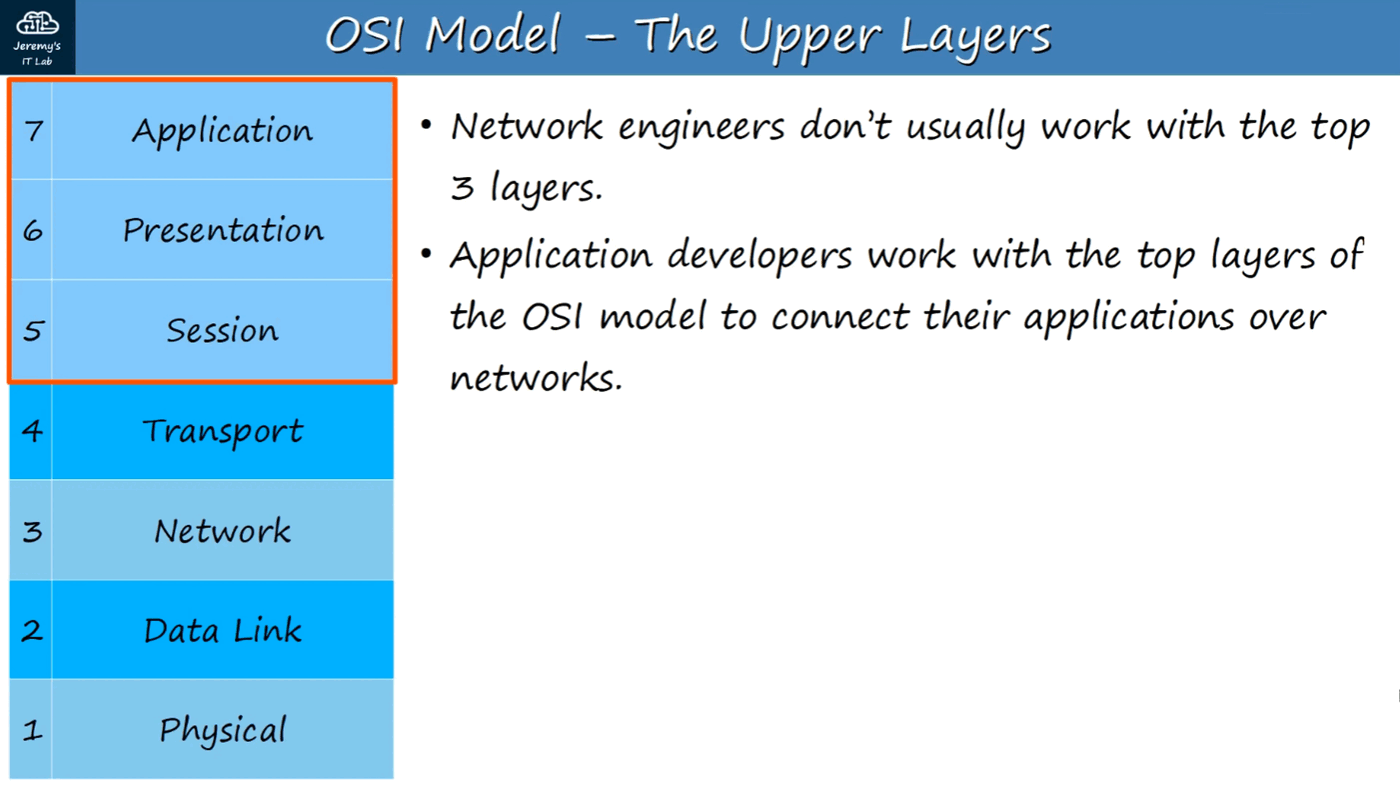
\includegraphics[keepaspectratio,alt={image}]{images/03-osi-model-tcpsuite/img-002.png}}
\end{figure}

Mnemonic to help remember the Data Layer Names / Order

\begin{figure}
\centering
\pandocbounded{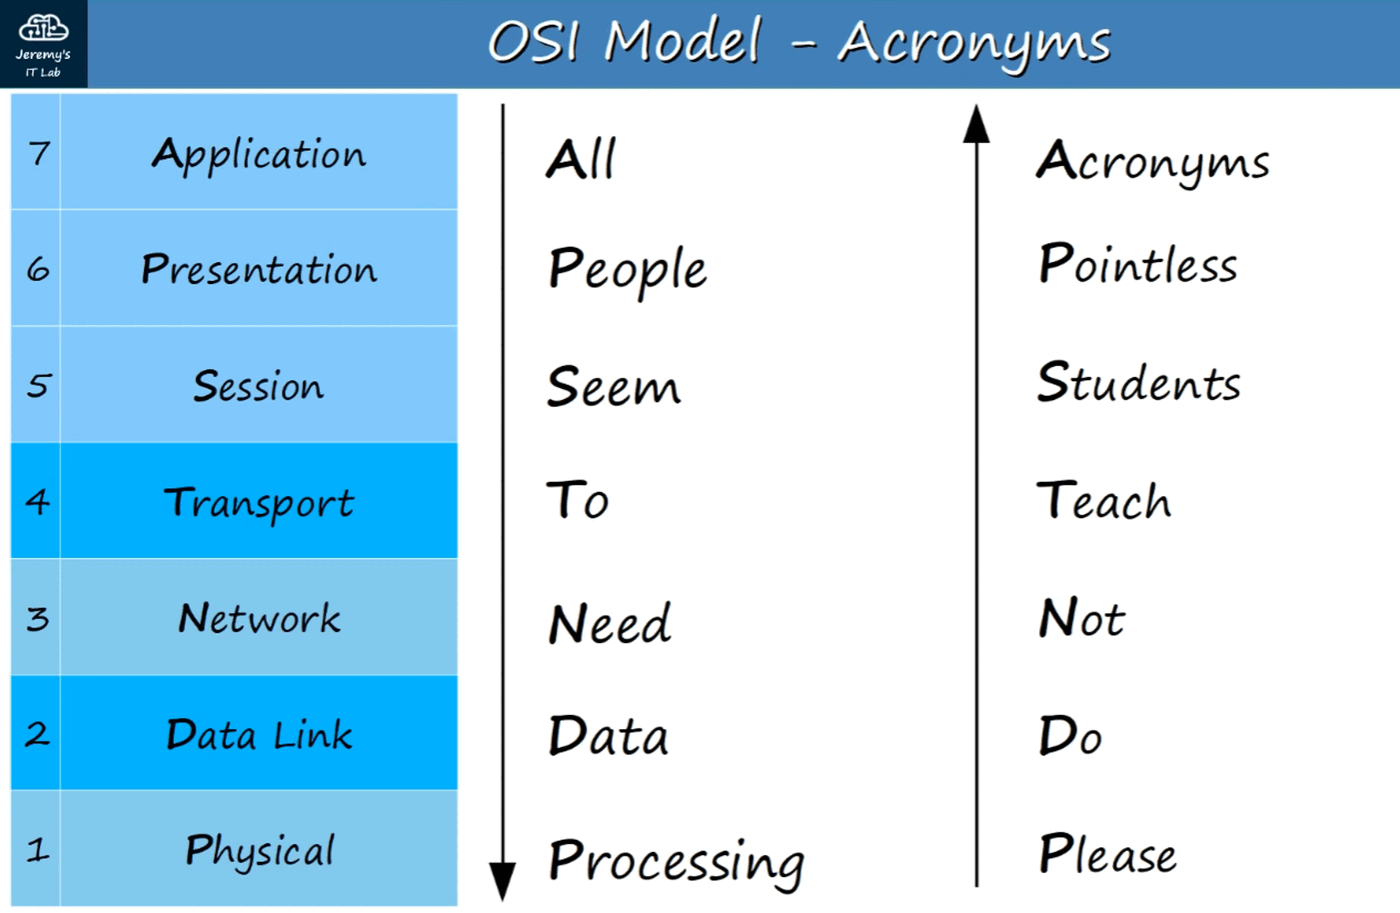
\includegraphics[keepaspectratio,alt={image}]{images/03-osi-model-tcpsuite/img-003.png}}
\end{figure}

\subsection{The layers are :}\label{the-layers-are}

\subsection{7 - APPLICATION}\label{application}

\begin{itemize}
\tightlist
\item
  This Layer is closest to end user.
\item
  Interacts with software applications.
\item
  HTTP and HTTPS are Layer 7 protocols
\end{itemize}

Functions of Layer 7 include:

\begin{itemize}
\tightlist
\item
  Identifying communication partners
\item
  Synchronizing communication
\end{itemize}

\subsection{6 - PRESENTATION}\label{presentation}

\begin{itemize}
\tightlist
\item
  Translates data to the appropriate format (between Application and
  Network formats) to be sent over the network.
\end{itemize}

\subsection{5 - SESSION}\label{session}

\begin{itemize}
\tightlist
\item
  Controls dialogues (sessions) between communicating hosts.
\item
  Establishes, manages, and terminates connections between local
  application and the remote application.
\end{itemize}

Network engineers don't usually work with the top 3 layers. Application
developers work with the top layers of the OSI model to connect their
applications over networks.

\subsection{4 - TRANSPORT}\label{transport}

\begin{itemize}
\tightlist
\item
  Segments and reassembles data for communication between end hosts.
\item
  Breaks large pieces of data into smaller segments which can be more
  easily sent over the network and are less likely to cause transmission
  problems if errors occur.
\item
  Provides HOST-TO-HOST (end to end) communication
\end{itemize}

When Data from Layer 7-5 arrives, it receives a Layer 4 Header in the
Transport layer.

\textless\textless{} DATA + L4 Header \textgreater\textgreater{}

This is called a SEGMENT.

\subsection{3 - NETWORK}\label{network}

\begin{itemize}
\tightlist
\item
  Provides connectivity between end hosts on different networks (ie:
  outside of the LAN).
\item
  Provides logical addressing (IP Addresses).
\item
  Provides path selection between source and destination
\item
  \textbf{ROUTERS} operate at Layer 3.
\end{itemize}

When Data and the Layer 4 Header arrive in the Network Layer, it
receives a Layer 3 Header.

\textless\textless{} DATA + L4 Header + L3 Header
\textgreater\textgreater{}

This is called a \textbf{PACKET}.

\subsection{2 - DATA LINK}\label{data-link}

\begin{itemize}
\tightlist
\item
  Provides NODE-TO-NODE connectivity and data transfer (for example, PC
  to Switch, Switch to Router, Router to Router)
\item
  Defines how data is formatted for transmission over physical medium
  (for example, copper UTP cables)
\item
  Detects and (possibly) corrects Physical (Layer 1) errors.
\item
  Uses Layer 2 addressing, separate from Layer 3 addressing.
\item
  \textbf{SWITCHES} operate at Layer 2
\end{itemize}

When the Layer 3 Packet arrives, a Layer 2 Trailer and Header are added.

\textless\textless{} L2 Trailer + DATA + L4 Header + L3 Header + L2
Header \textgreater\textgreater{}

This is called a FRAME.

All the steps leading up to transmission is called ENCAPSULATION. When
the frame is sent to the receiver, it then goes through the reverse
process, DE-ENCAPSULATION, stripping off layers while travelling from
OSI Layer 1 to Layer 7.

\subsection{1 - PHYSICAL}\label{physical}

\begin{itemize}
\tightlist
\item
  Defines physical characteristics of the medium used to transfer data
  between devices. For example : voltage levels, maximum transmission
  distances, physical connectors, cable specs.
\item
  Digital bits are converted into electrical (for wired connections) or
  radio (for wireless connections) signals.
\item
  All of the information in SECTION 2 (NETWORKING DEVICES) is related to
  the Physical Layer
\end{itemize}

\subsection{OSI MODEL - PDU's}\label{osi-model---pdus}

\begin{figure}
\centering
\pandocbounded{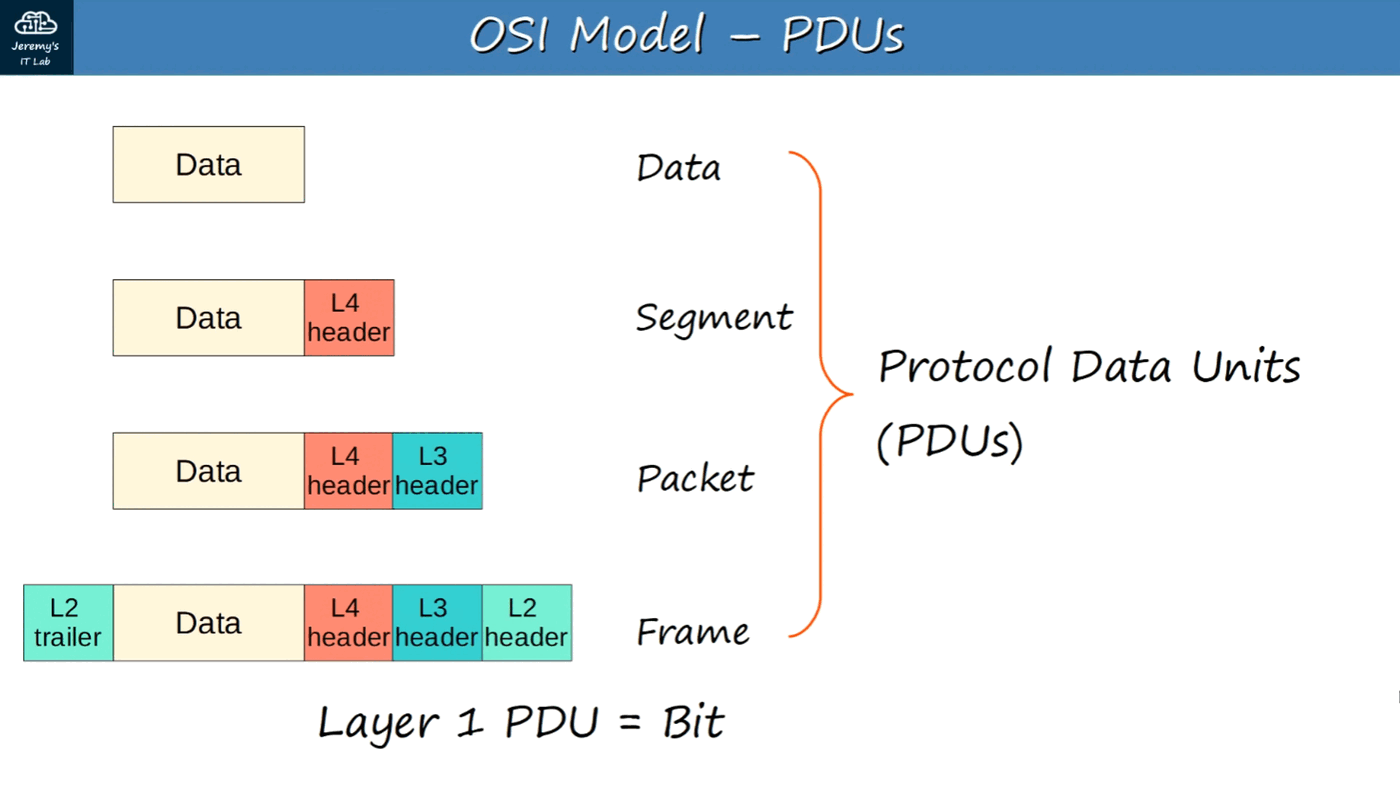
\includegraphics[keepaspectratio,alt={image}]{images/03-osi-model-tcpsuite/img-004.png}}
\end{figure}

A PDU is a Protocol Data Unit. Each step of the process is a PDU.

{\def\LTcaptype{none} % do not increment counter
\begin{longtable}[]{@{}lll@{}}
\toprule\noalign{}
OSI LAYER \# & PDU NAME & PROTOCOL DATA ADDED \\
\midrule\noalign{}
\endhead
\bottomrule\noalign{}
\endlastfoot
7-5 & DATA & Data \\
4 & SEGMENT & Layer 4 Header Added \\
3 & PACKET & Layer 3 Header Added \\
2 & FRAME & Layer 2 Trailer and Header Added \\
1 & BIT & 0s and 1s Transmission \\
\end{longtable}
}

\textless\textless{} L2 Trailer + DATA + L4 Header + L3 Header + L2
Header \textgreater\textgreater{}

\subsection{TCP/IP Suite}\label{tcpip-suite}

\begin{itemize}
\tightlist
\item
  Conceptual model and set of communications protocols used in the
  Internet and other networks.
\item
  Known as TCP/IP because those are two of the foundational protocols in
  the suite.
\item
  Developed by the US Dept. of Defense through DARPA (Defense Advanced
  Research Projects Agency).
\item
  Similar structure to the OSI Model, but fewer layers.
\item
  THIS is the model actually in use in modern networks.
\item
  \begin{itemize}
  \tightlist
  \item
    Note : The OSI Model still influences how network engineers think
    and talk about networks.
  \end{itemize}
\end{itemize}

\begin{figure}
\centering
\pandocbounded{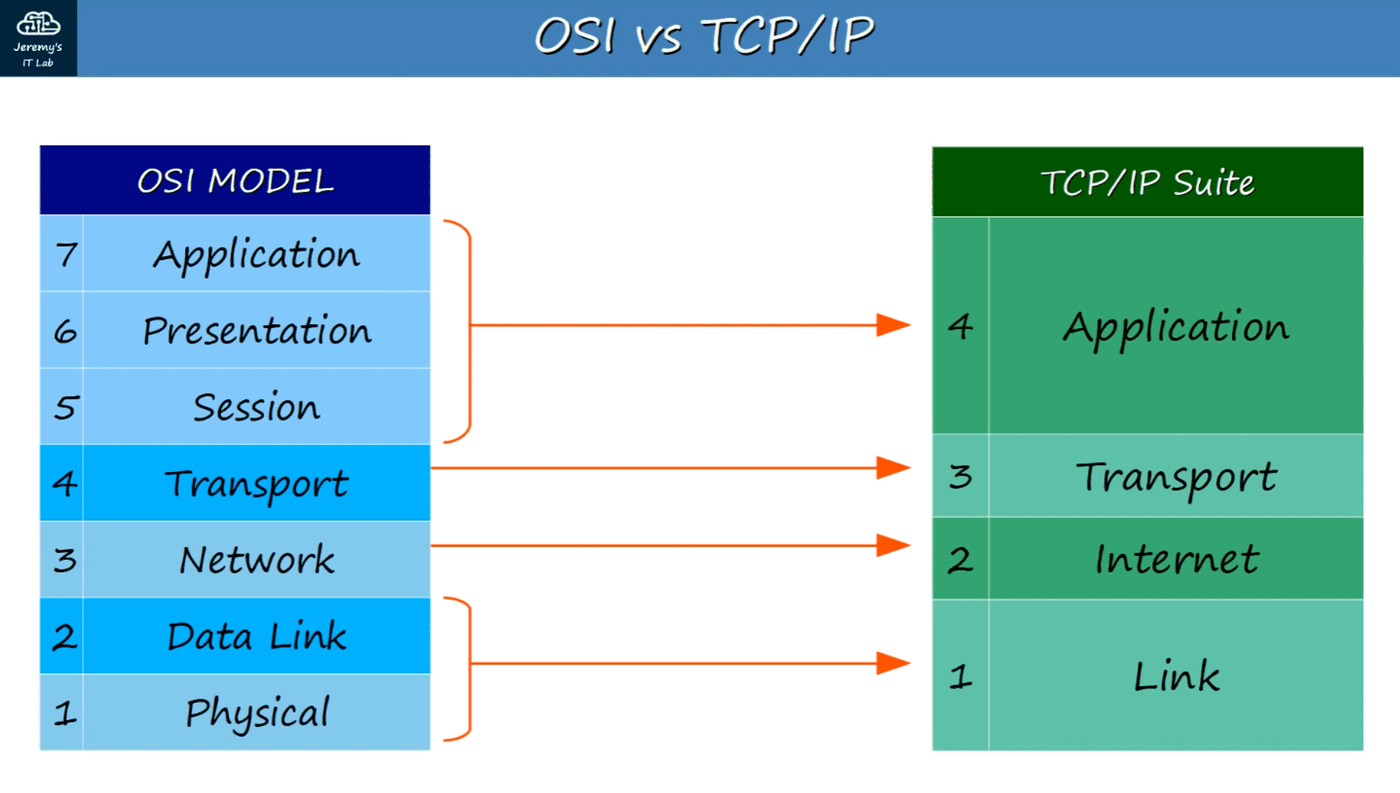
\includegraphics[keepaspectratio,alt={image}]{images/03-osi-model-tcpsuite/img-005.png}}
\end{figure}

\subsection{Layer Interactions}\label{layer-interactions}

\begin{figure}
\centering
\pandocbounded{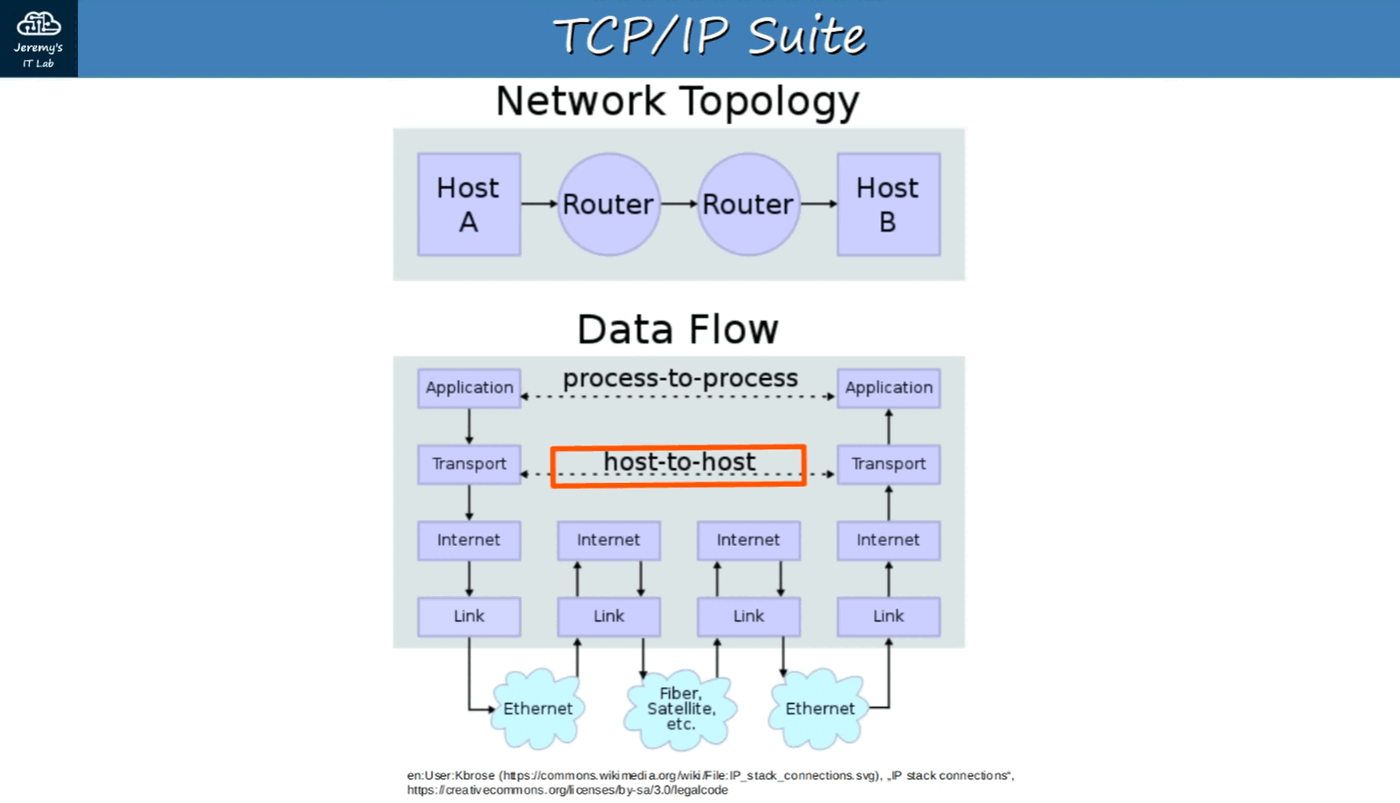
\includegraphics[keepaspectratio,alt={image}]{images/03-osi-model-tcpsuite/img-006.png}}
\end{figure}

Adjacent-Layer Interactions:

\begin{itemize}
\tightlist
\item
  Interactions between different layers of the OSI Model on same host.
\end{itemize}

Example:

Layers 5-7 sending Data to Layer 4, which then adds a Layer 4 header
(creating a SEGMENT).

Same-Layer Interactions:

\begin{itemize}
\tightlist
\item
  Interactions between the same Layer on different hosts.
\item
  The concept of Same-Layer interaction allows you to ignore the other
  layers involved and focus on the interactions between a single layer
  on different devices.
\end{itemize}

Example:

The Application Layer of YouTube's web server and your PC's browser.

\chapter{Introduction to the CLI}\label{introduction-to-the-cli}

\subsection{What is a CLI?}\label{what-is-a-cli}

\begin{itemize}
\tightlist
\item
  A ``Command-line Interface''
\item
  The interface you use to configure Cisco devices
\end{itemize}

A GUI is a ``Graphical User Interface''

\subsection{How do you connect to a Cisco
Device?}\label{how-do-you-connect-to-a-cisco-device}

\begin{itemize}
\tightlist
\item
  Console Port : When you first configure a device, you have to connect
  via the Console Port.
\end{itemize}

You can use a ``Rollover cable'' : DB9 serial connector to RJ45 OR a DB9
Serial to USB

\begin{figure}
\centering
\pandocbounded{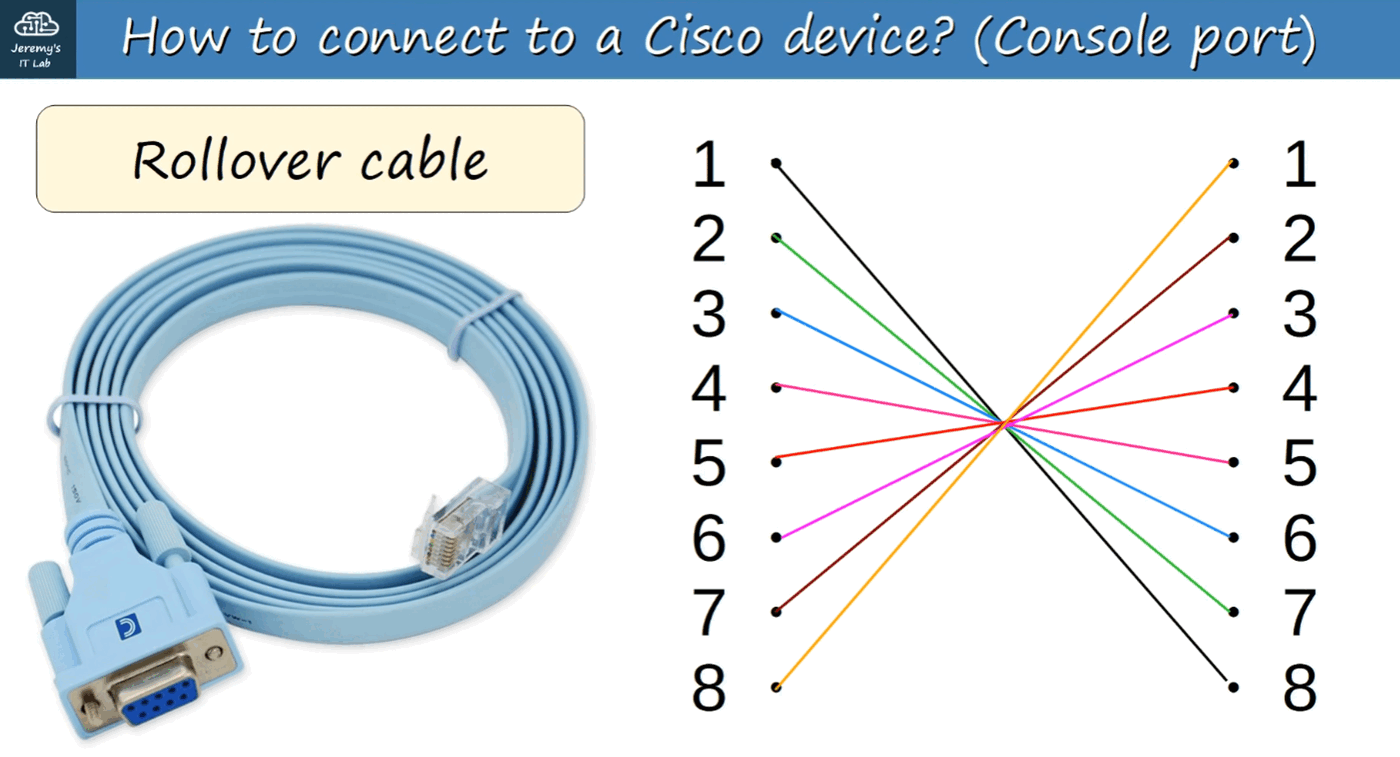
\includegraphics[keepaspectratio,alt={image}]{images/04-intro-to-cli/img-001.png}}
\end{figure}

\subsection{How do you actually access the
CLI?}\label{how-do-you-actually-access-the-cli}

\begin{itemize}
\tightlist
\item
  You need to use a TERMINAL EMULATOR (Example: PuTTy is a popular
  choice) and connect via ``Serial'' (default settings)
\end{itemize}

\subsection{Cisco Default Settings
are:}\label{cisco-default-settings-are}

Speed (baud) : 9600 bits/second Data bits: 8 data bits Stop bits: 1 stop
bit (sent after 8 data bits are sent) Parity: None Flow Control: None

When you first enter the CLI you will DEFAULT be in what is called `User
EXEC' mode.

\section{User Exec Mode}\label{user-exec-mode}

\begin{lstlisting}
(Hostname) >        // Prompt looks like THIS //
\end{lstlisting}

\begin{itemize}
\tightlist
\item
  User EXEC mode is very limited.
\item
  User can look at some things but can't make ANY changes to the
  configuration.
\item
  AKA `User Mode'
\end{itemize}

Using the `enable' command, in User EXEC mode, switches you to
`Privileged EXEC' mode.

\section{Privileged Exec Mode}\label{privileged-exec-mode}

\begin{itemize}
\tightlist
\item
  Provides complete access to view the device's configuration, restart
  the device, etc.
\item
  Cannot change the configuration, but can change the time on the
  device, save the configuration file, etc.
\end{itemize}

\begin{lstlisting}
(Hostname)#     // Prompt looks like THIS //
\end{lstlisting}

USE a Question Mark (?) to view the available commands in ANY mode.
Combining ? with a letter or partial command will list all the commands
with those letters.

\begin{figure}
\centering
\pandocbounded{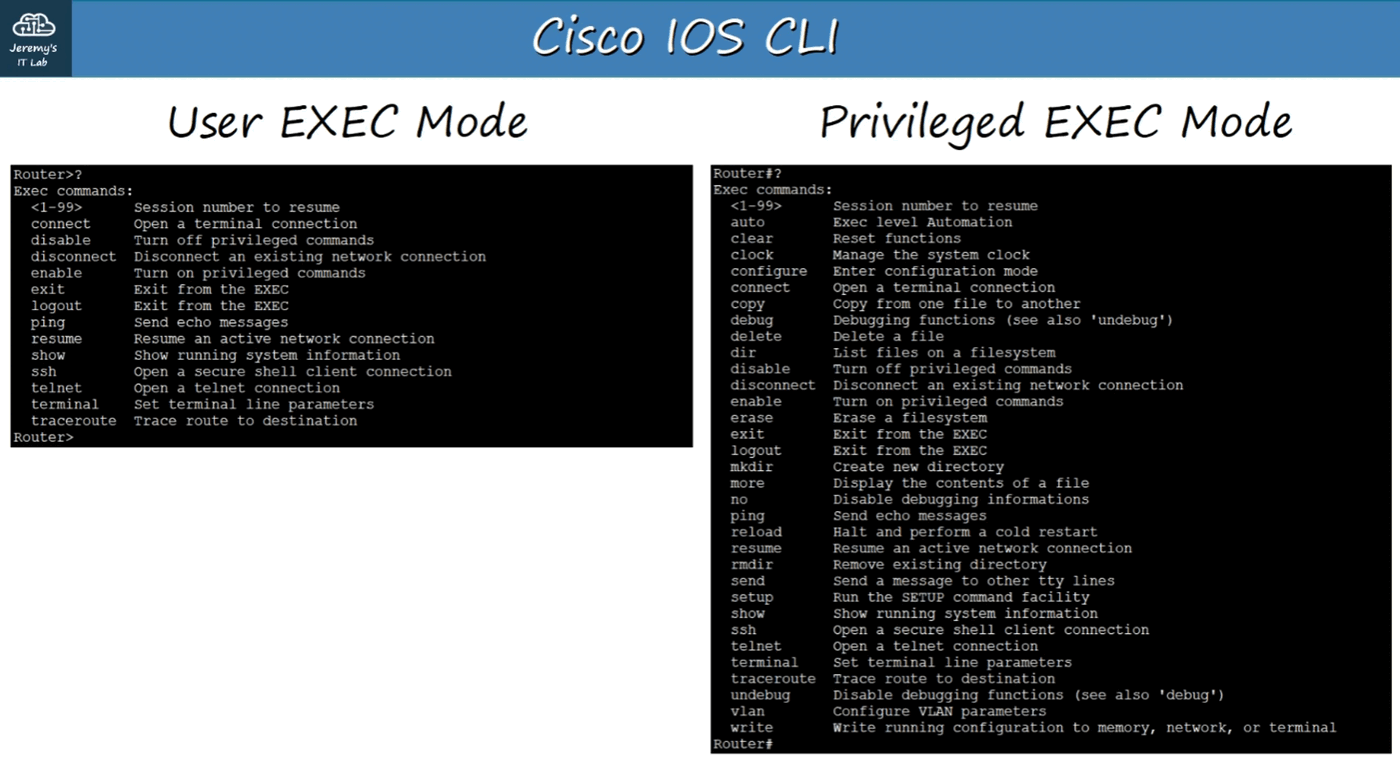
\includegraphics[keepaspectratio,alt={image}]{images/04-intro-to-cli/img-002.png}}
\end{figure}

USE the TAB key to complete partially entered commands IF the command
exists.

\subsection{GLOBAL CONFIGURATION MODE:}\label{global-configuration-mode}

To enter Global Configuration Mode, enter the command, within Privileged
EXEC mode

`configure terminal' (or `conf t')

Router\# configure terminal

Note the prompt change:

Router(config) \#

Type `exit' to drop back into `Privileged EXEC' mode.

\subsection{To Enable Password for User EXEC
mode:}\label{to-enable-password-for-user-exec-mode}

Router(config)\# enable password (password)

\begin{itemize}
\tightlist
\item
  Passwords ARE case-sensitive.
\end{itemize}

// This command encrypts plain-text passwords, visible in the config
files, using simple encryption.

Router(config)\# service password-encryption

If you enable `service password-encryption'

\begin{itemize}
\tightlist
\item
  Current passwords WILL be encrypted.
\item
  Future passwords WILL be encrypted.
\item
  The `enable secret' WILL NOT be effected.
\end{itemize}

If you disable `service password-encryption'

\begin{itemize}
\tightlist
\item
  Current passwords WILL NOT be decrypted.
\item
  Future passwords WILL NOT be encrypted.
\item
  The `enable secret' WILL NOT be effected.
\end{itemize}

// This command enables passwords for the Privileged EXEC mode.

Router(config)\# enable secret (password)

// enable secret will ALWAYS be encrypted (at level 5)

There are TWO separate configuration files kept on the device at once.

Running-config :

\begin{itemize}
\tightlist
\item
  The current, ACTIVE configuration file on the device. As you enter
  commands in the CLI, you edit the active configuration.
\end{itemize}

Startup-config :

\begin{itemize}
\tightlist
\item
  The configuration file that will be loaded upon RESTART of the device.
\end{itemize}

To see the configuration files, inside `Privileged EXEC' mode:

Router\# show running-config // for running config //

OR

Router\# show startup-config // for startup config //

To SAVE the Running configuration file, you can:

Router\# write Building configuration\ldots{} {[}OK{]}

Router\# write memory Building configuration\ldots{} {[}OK{]}

Router\# copy running-config startup-config

Destination filename {[}startup-config{]}?

Building configuration\ldots{} {[}OK{]}

To encrypt passwords:

Router\# conf t

Router(config)\# service password-encryption

This makes all current passwords \emph{encrypted}

Future passwords will ALSO be \emph{encrypted}

``Enable secret'' will not be effected (it's ALWAYS encrypted)

\begin{figure}
\centering
\pandocbounded{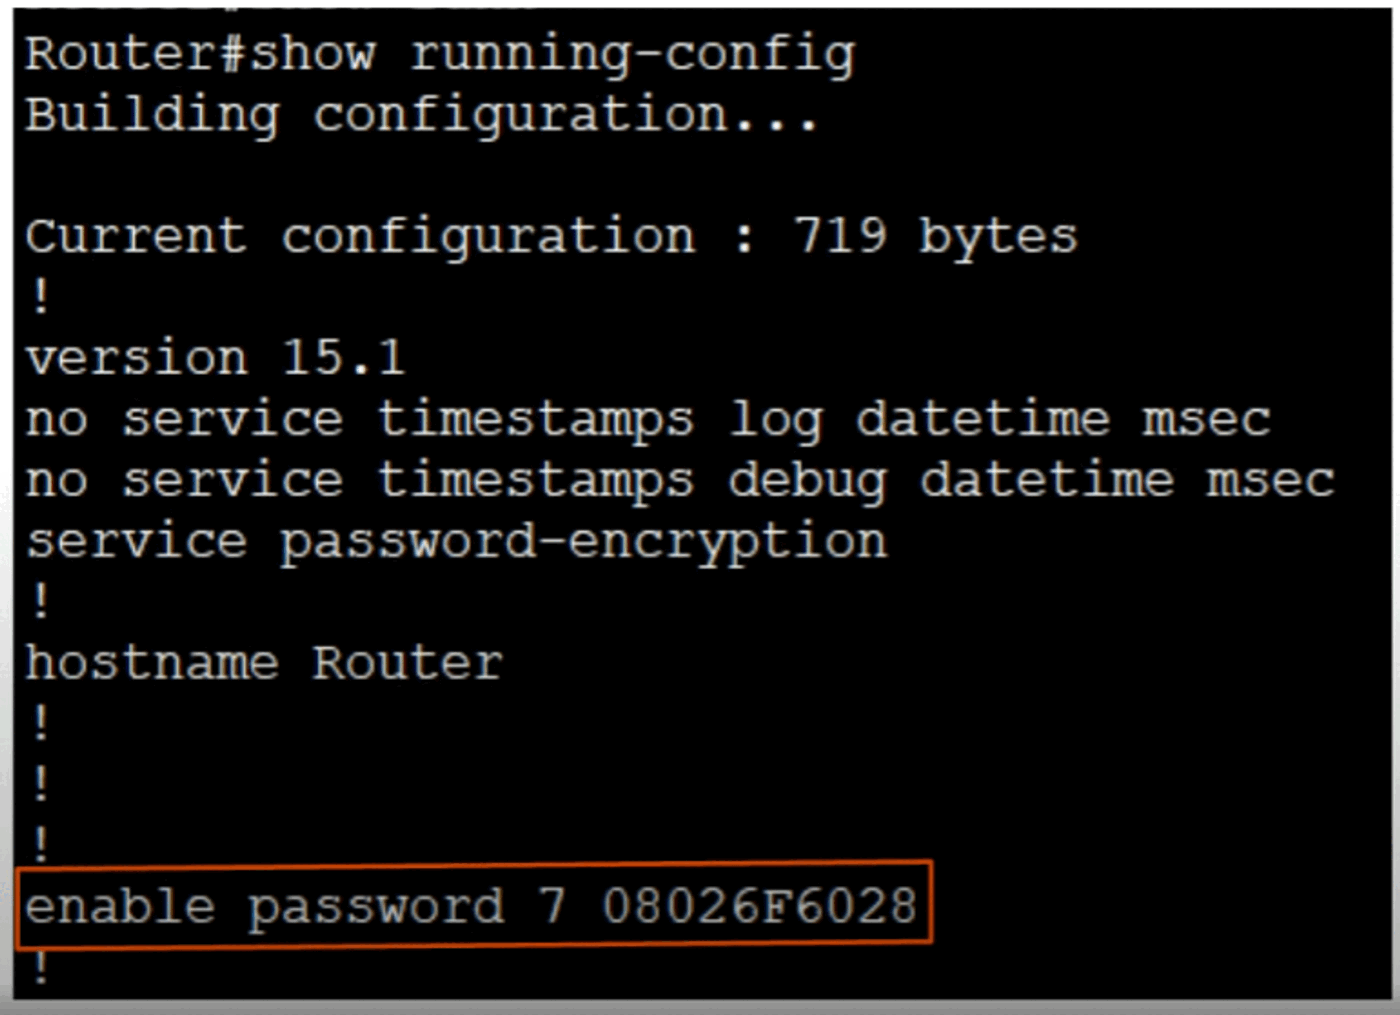
\includegraphics[keepaspectratio,alt={image}]{images/04-intro-to-cli/img-003.png}}
\end{figure}

Now you will see that the password is no longer in plaintext.

``7'' refers to the type of encryption used to encrypt the password. In
this case, ``7'' uses Cisco's proprietary encryption.

``7'' is fairly easy to crack since the encryption is weak.

For BETTER / STRONGER encryption, use ``enable secret''

\begin{figure}
\centering
\pandocbounded{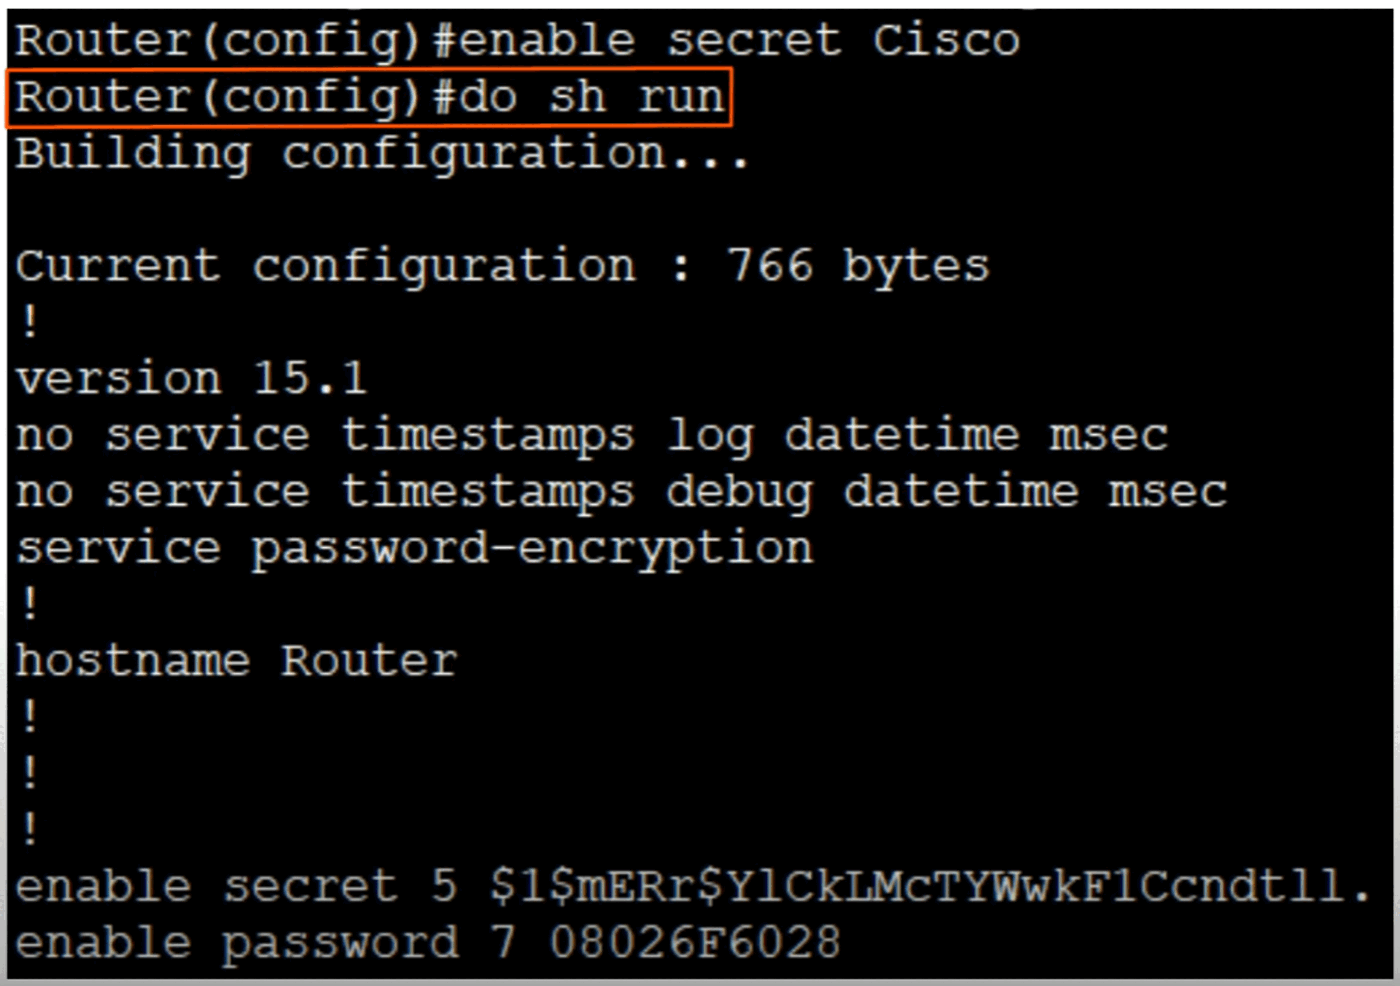
\includegraphics[keepaspectratio,alt={image}]{images/04-intro-to-cli/img-004.png}}
\end{figure}

``5'' refers to MD5 encryption.

Can still be cracked but it's much much stronger.

Once you use ``enable secret'' command, this will override ``enable
password''

To CANCEL or delete a command you entered, use the ``no'' keyword

\begin{figure}
\centering
\pandocbounded{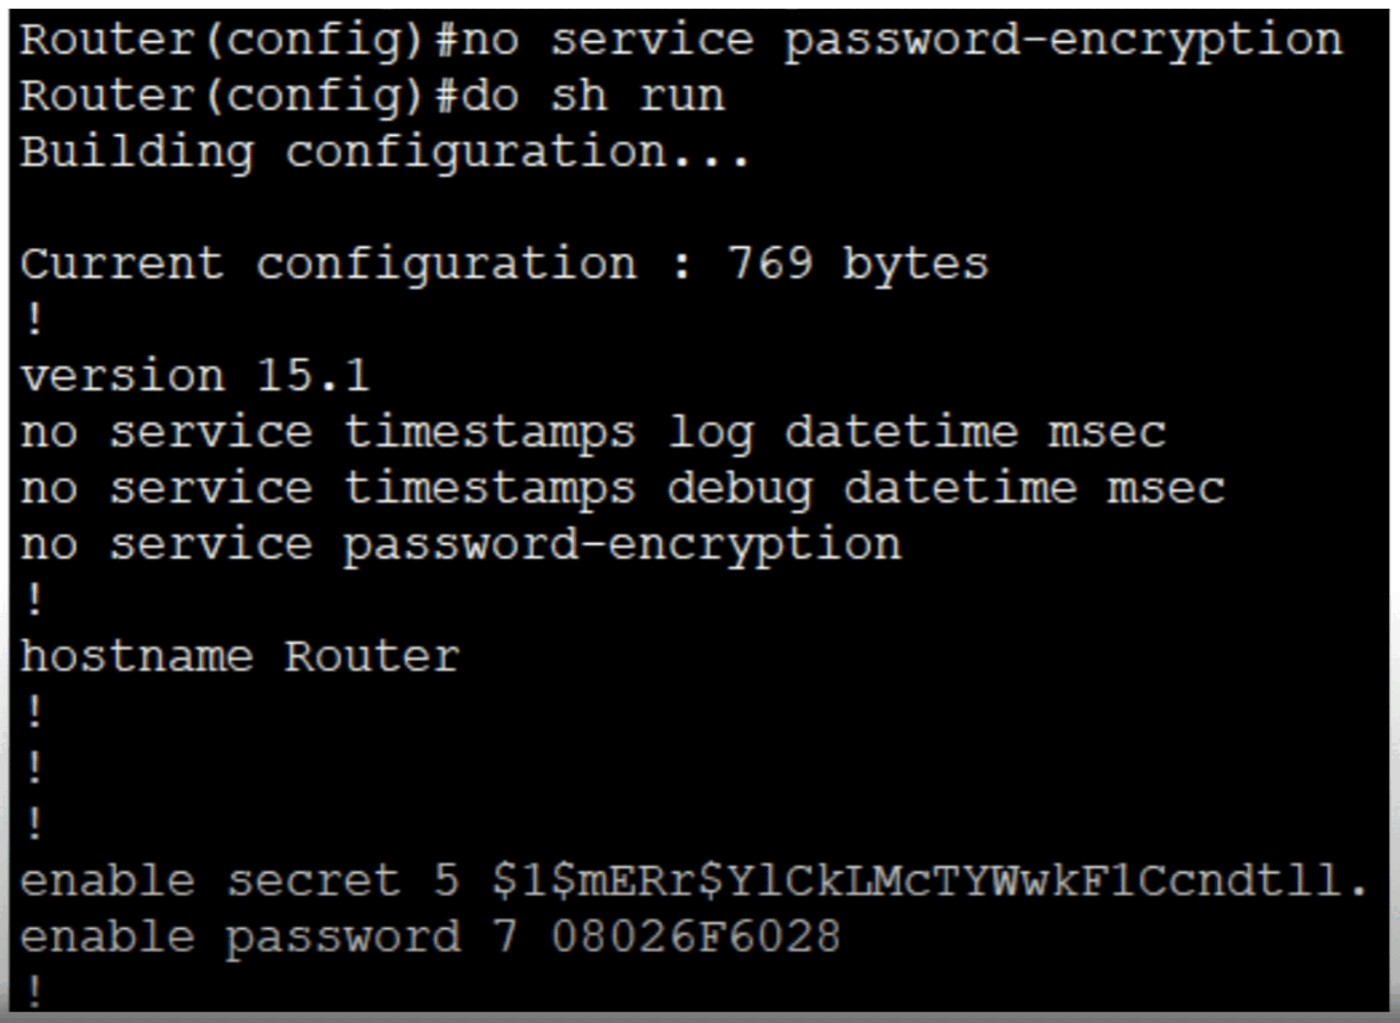
\includegraphics[keepaspectratio,alt={image}]{images/04-intro-to-cli/img-005.png}}
\end{figure}

In this instance, disabling ``service password-encryption'':

\begin{itemize}
\tightlist
\item
  current passwords will NOT be decrypted (unchanged)
\item
  future passwords will NOT be encrypted
\item
  the ``enable secret'' will not be effected
\end{itemize}

\begin{figure}
\centering
\pandocbounded{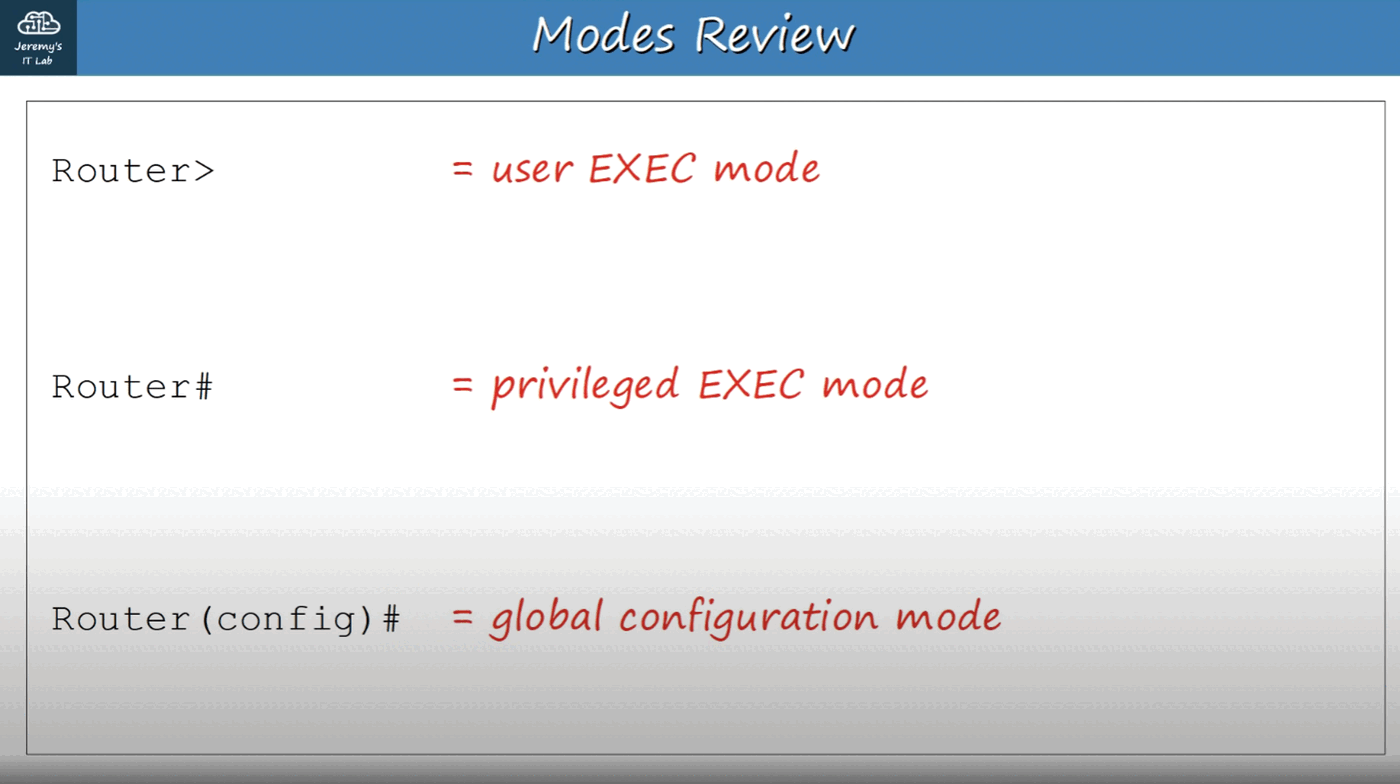
\includegraphics[keepaspectratio,alt={image}]{images/04-intro-to-cli/img-006.png}}
\end{figure}

\begin{figure}
\centering
\pandocbounded{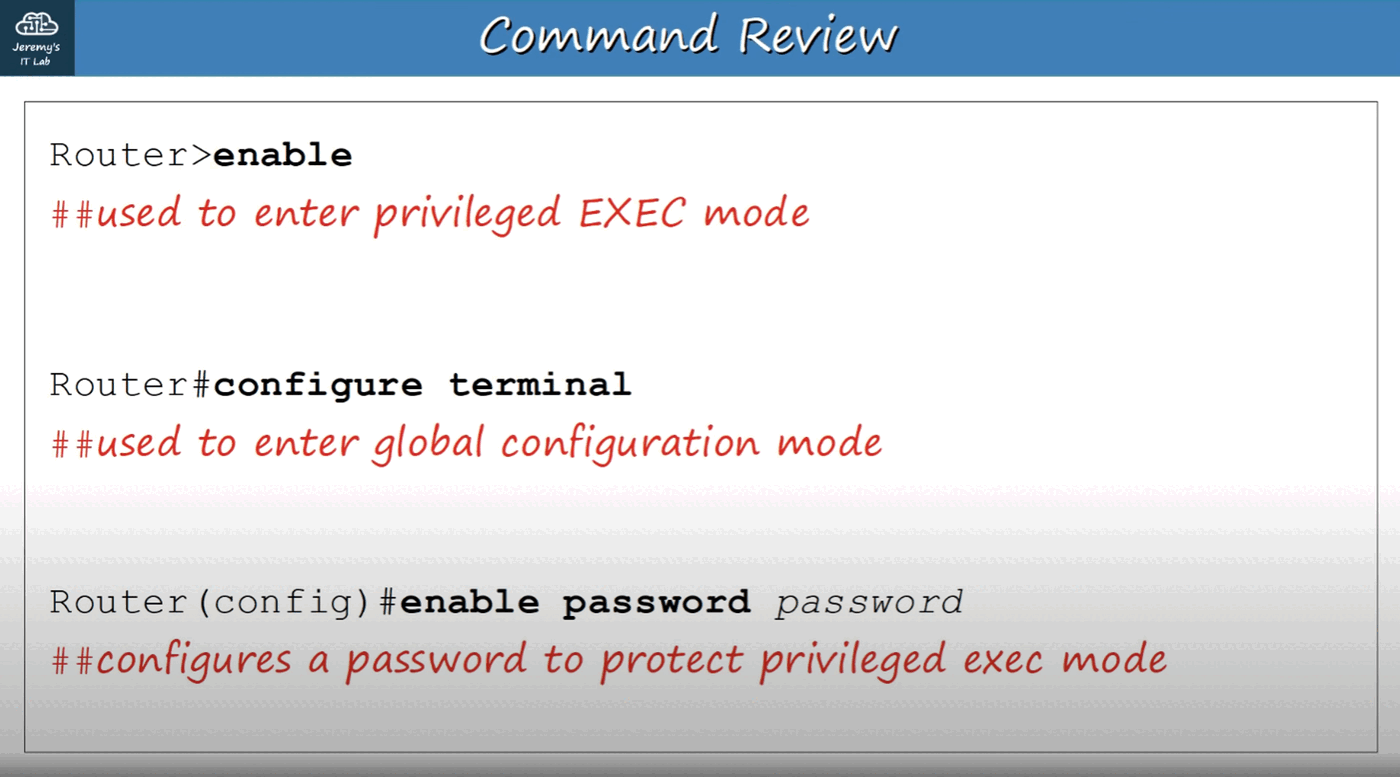
\includegraphics[keepaspectratio,alt={image}]{images/04-intro-to-cli/img-007.png}}
\end{figure}

\begin{figure}
\centering
\pandocbounded{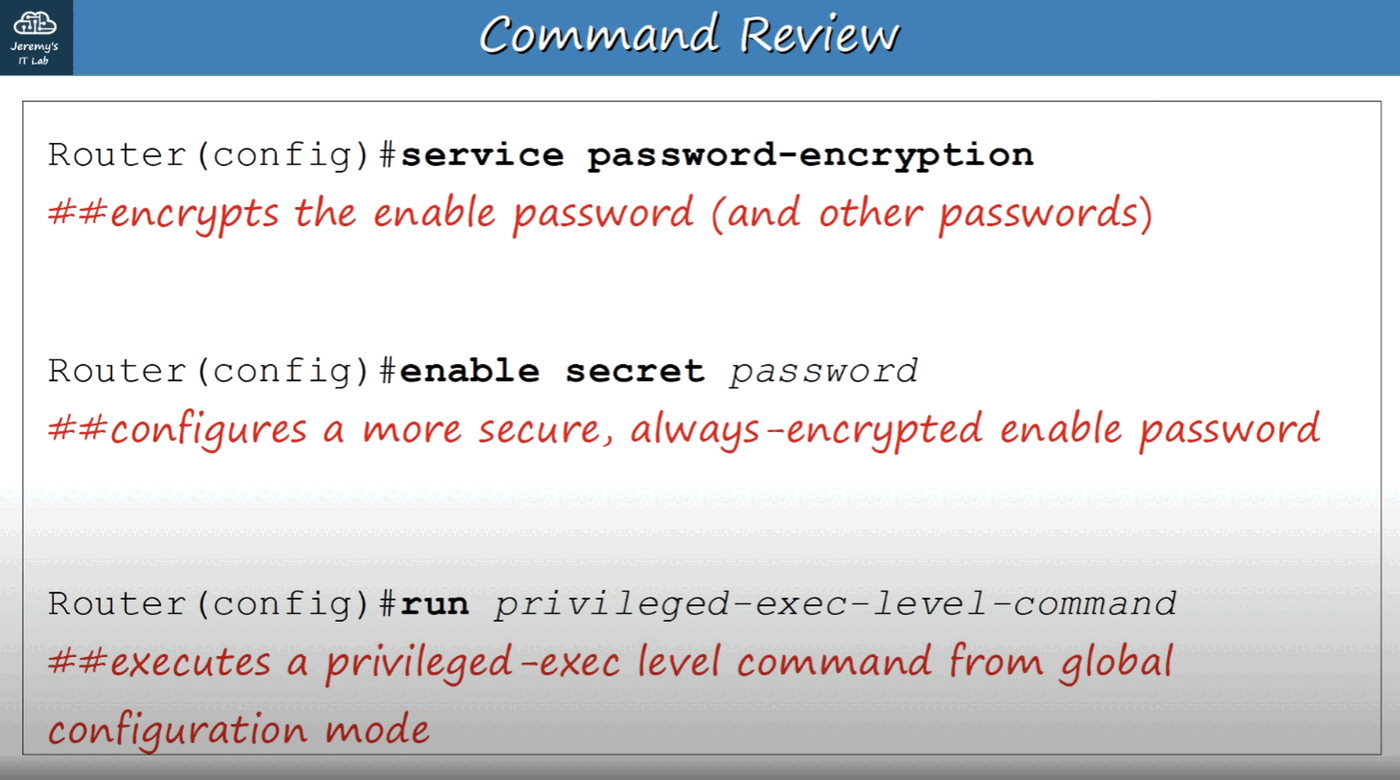
\includegraphics[keepaspectratio,alt={image}]{images/04-intro-to-cli/img-008.png}}
\end{figure}

\begin{figure}
\centering
\pandocbounded{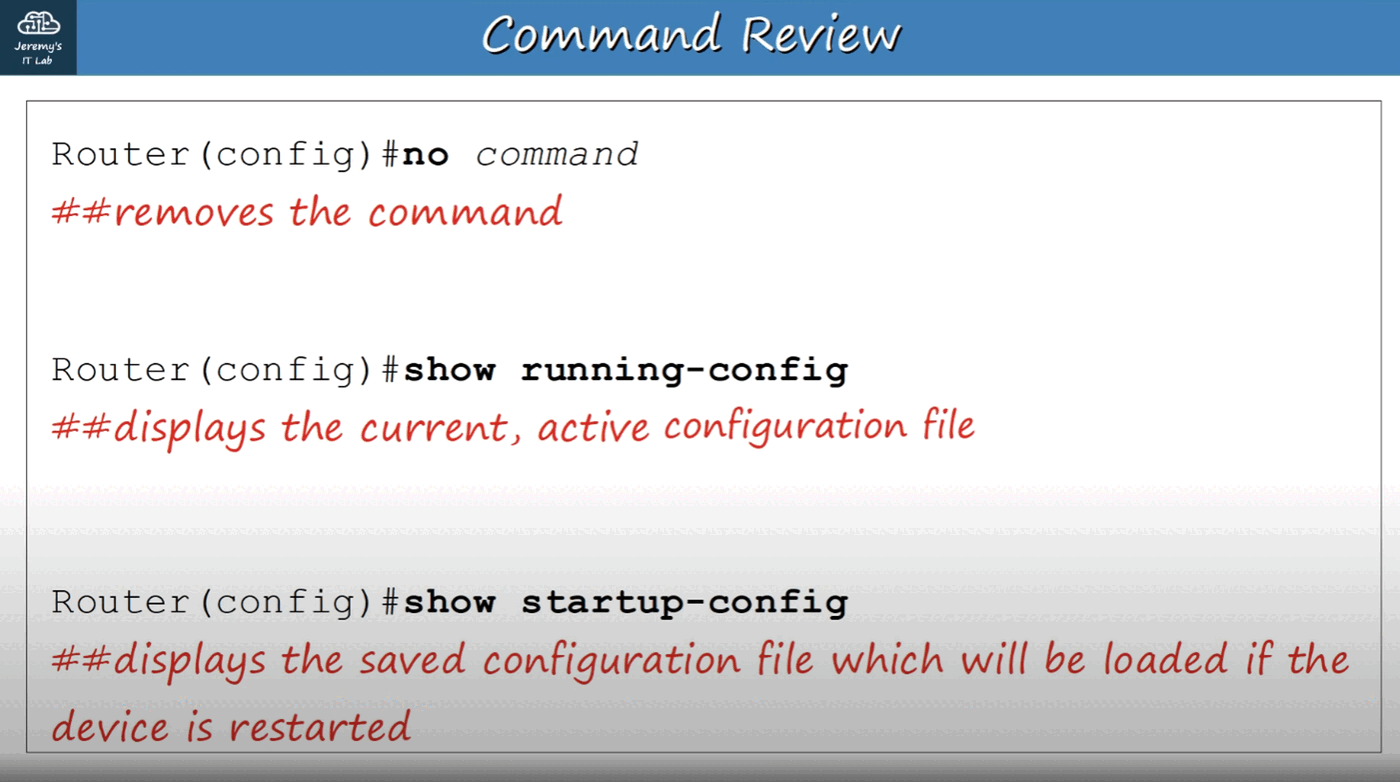
\includegraphics[keepaspectratio,alt={image}]{images/04-intro-to-cli/img-009.png}}
\end{figure}

\begin{figure}
\centering
\pandocbounded{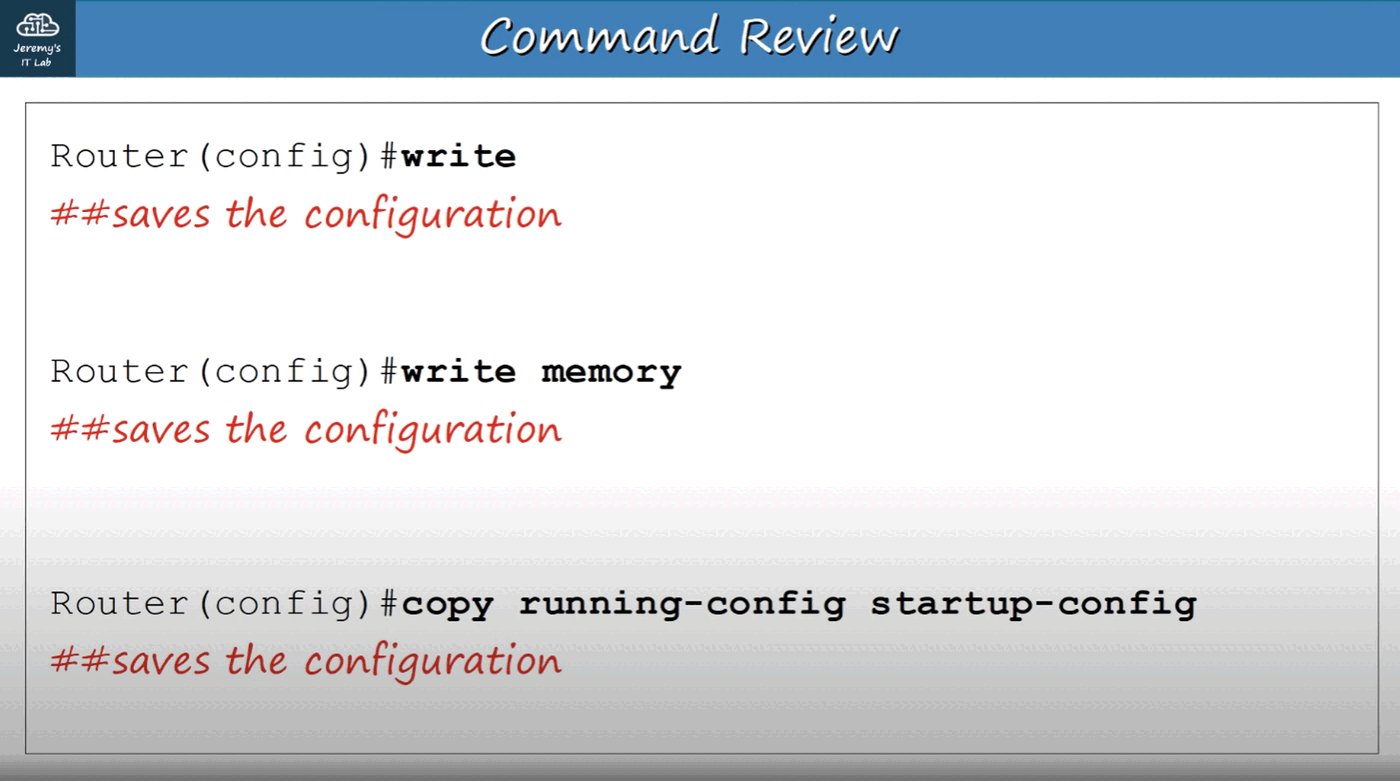
\includegraphics[keepaspectratio,alt={image}]{images/04-intro-to-cli/img-010.png}}
\end{figure}

\chapter{Ethernet LAN Switching: Part
1}\label{ethernet-lan-switching-part-1}

\begin{figure}
\centering
\pandocbounded{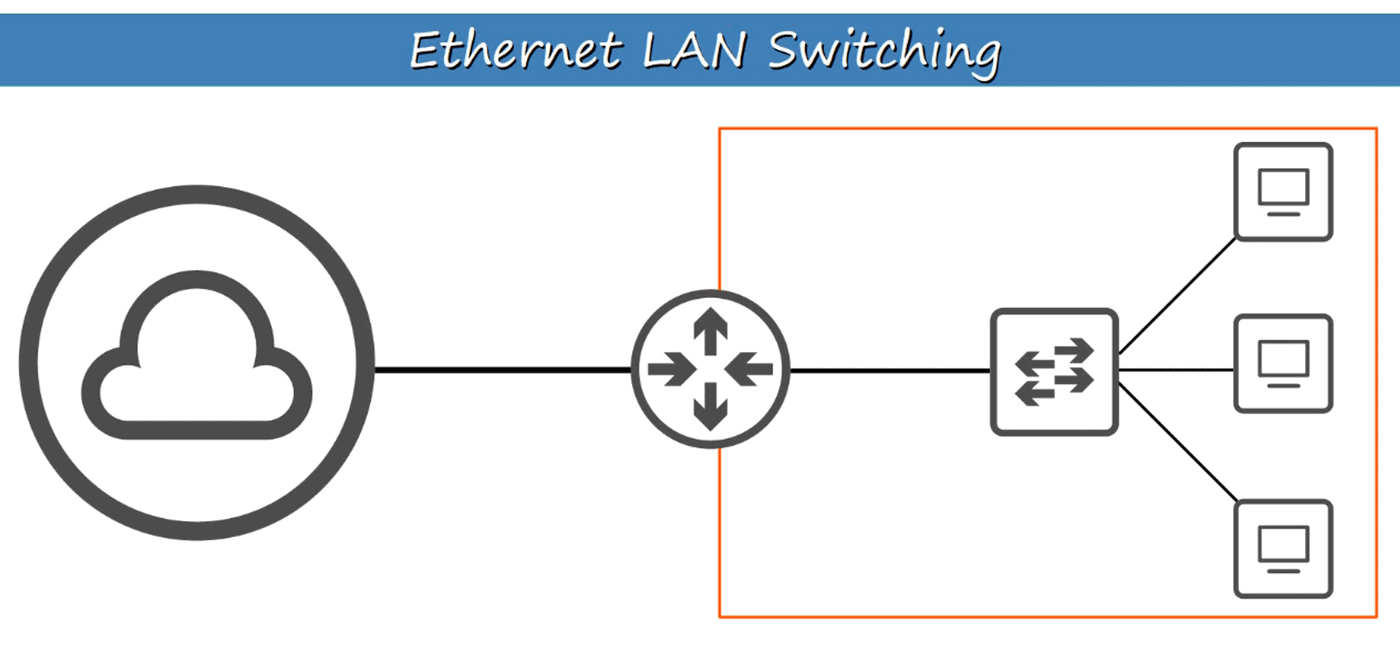
\includegraphics[keepaspectratio,alt={image}]{images/05-ethernet-lan-switching-part1/img-001.png}}
\end{figure}

\begin{figure}
\centering
\pandocbounded{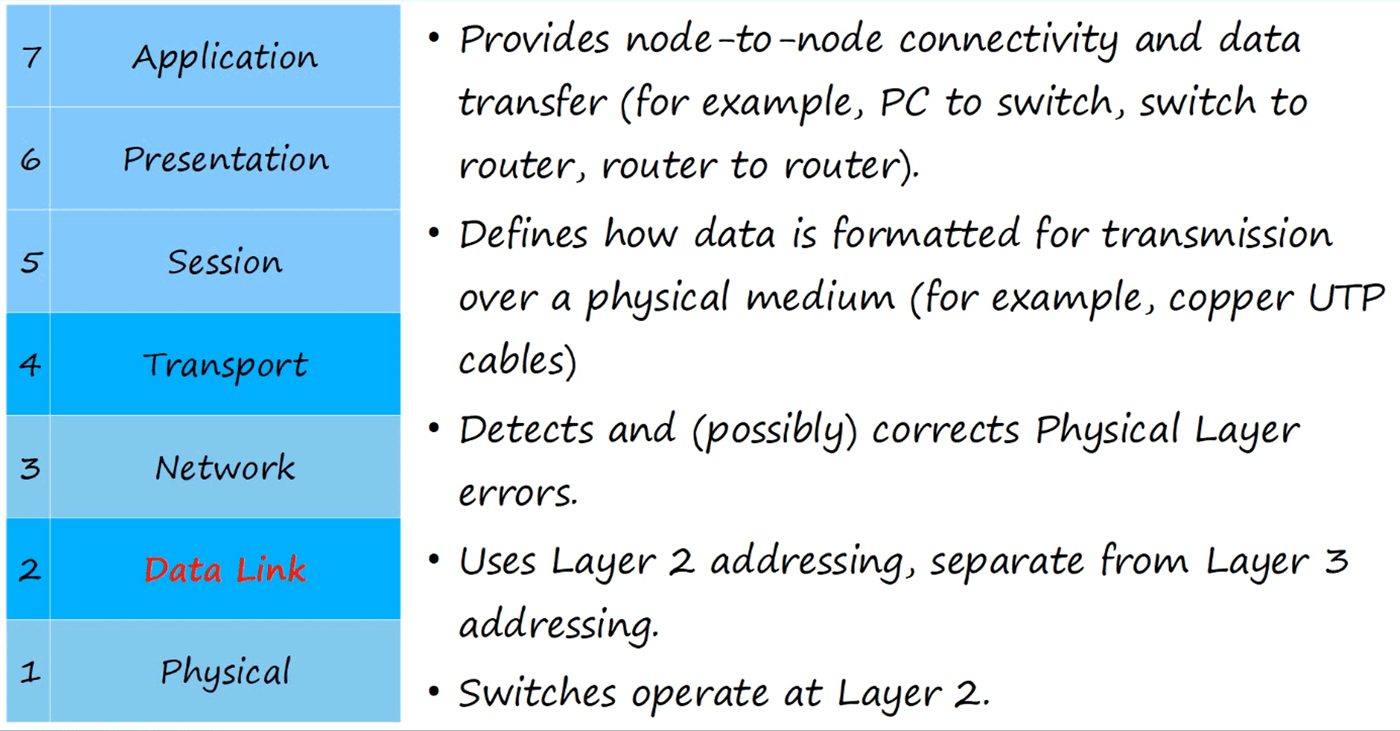
\includegraphics[keepaspectratio,alt={image}]{images/05-ethernet-lan-switching-part1/img-002.png}}
\end{figure}

LAN's

\begin{itemize}
\tightlist
\item
  A LAN is a network contained in a relatively small area.
\item
  Routers are used to connect separate LAN's
\end{itemize}

\begin{figure}
\centering
\pandocbounded{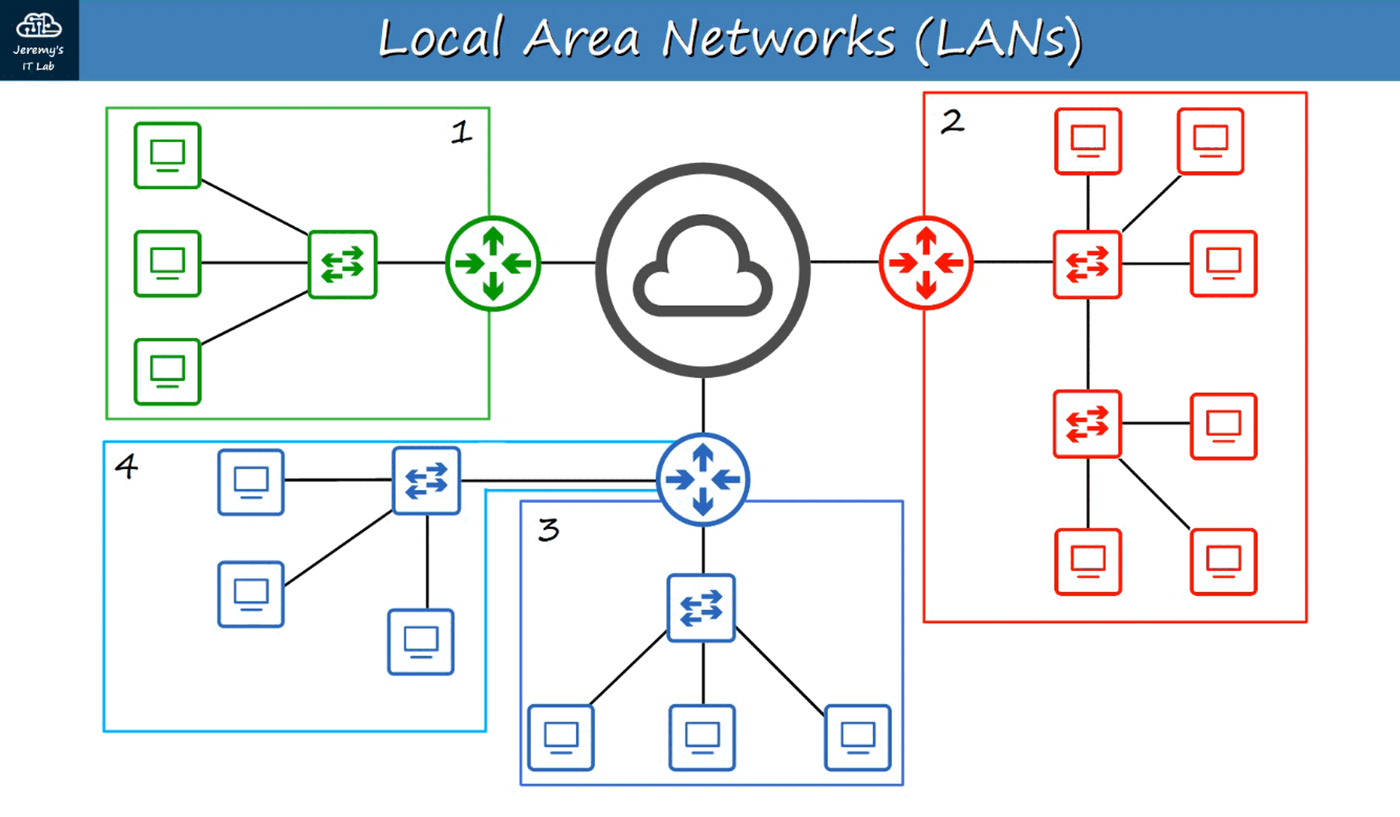
\includegraphics[keepaspectratio,alt={image}]{images/05-ethernet-lan-switching-part1/img-003.png}}
\end{figure}

An ETHERNET FRAME looks like:

\begin{figure}
\centering
\pandocbounded{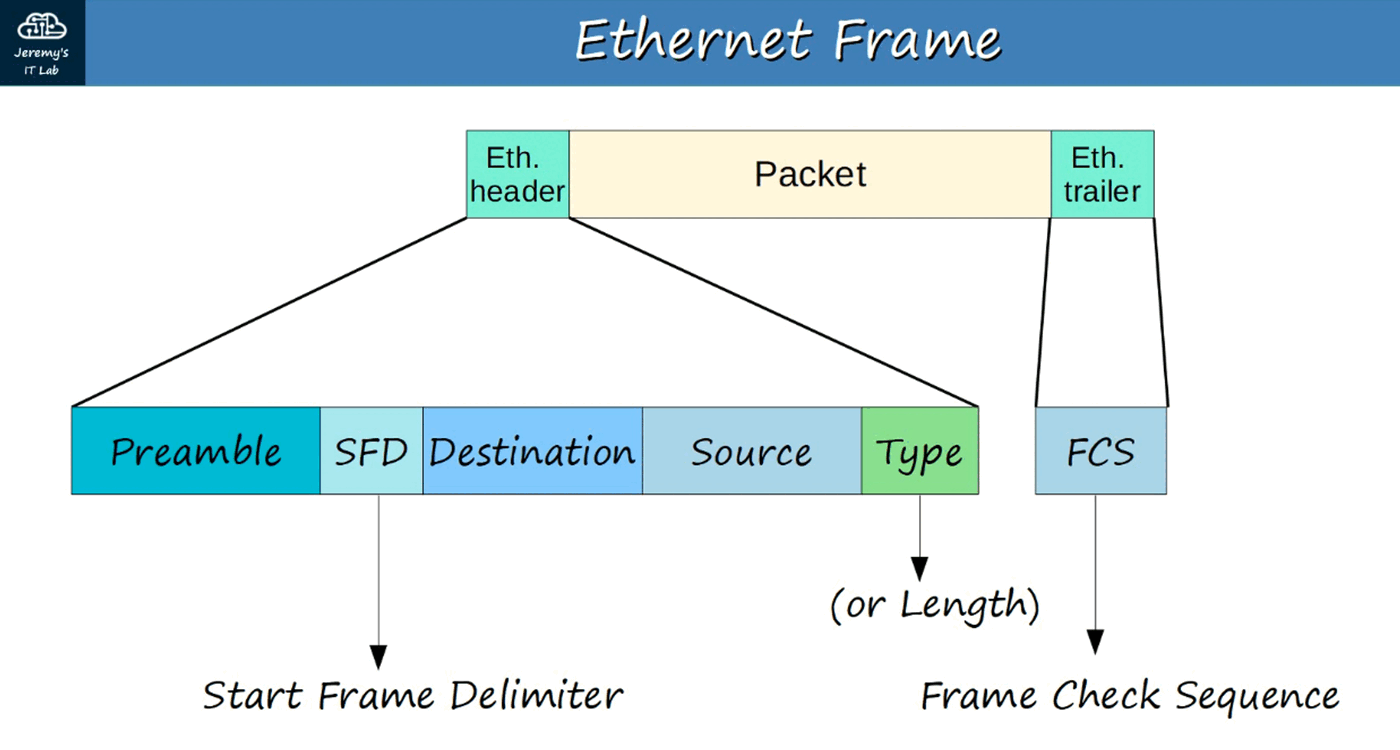
\includegraphics[keepaspectratio,alt={image}]{images/05-ethernet-lan-switching-part1/img-004.png}}
\end{figure}

Ethernet Trailer --- PACKET --- Ethernet Header

The Ethernet Header contains 5 Fields:

Preamble -- SFD -- Destination -- Source -- Type 7 bytes -- 1 byte -- 6
bytes -- 6 bytes -- 2 bytes

\section{Preamble}\label{preamble}

\begin{itemize}
\tightlist
\item
  Length: 7 bytes (56 bits)
\item
  Alternating 1's and 0's
\item
  10101010 * 7x
\item
  Allows devices to synchronize their receiver clocks
\end{itemize}

SFD : `Start Frame Delimiter'

\begin{itemize}
\tightlist
\item
  Length: 1 byte(8 bits)
\item
  10101011
\item
  Marks end of the PREAMBLE and beginning of rest of frame.
\end{itemize}

\section{Destination and Source}\label{destination-and-source}

\begin{itemize}
\tightlist
\item
  Layer 2 Address
\item
  Indicates the devices sending / receiving the frame
\item
  MAC = 'Media Access Control'
\item
  = 6 byte (48-bit) address of the physical device
\end{itemize}

\section{Type / Length}\label{type-length}

\begin{itemize}
\tightlist
\item
  2 bytes (16-bit) field
\item
  A value of 1\textbf{500 or less} in this field indicates the LENGTH of
  the encapsulated packet (in bytes)
\item
  A value of \textbf{1536 or greater} in this field indicates the TYPE
  of the encapsulated packet and length is determined via other methods.
\item
  IPv4 = 0x0800 (hexadecimal) = 2048 in decimal
\item
  IPv6 = 0x86DD (hexadecimal) = 34525 in decimal
\item
  Layer 3 protocol used in the encapsulated Packet, which is almost
  always Internet Protocol (IP) version 4 or version 6.
\end{itemize}

The ETHERNET TRAILER contains:

\section{Fcs}\label{fcs}

\begin{itemize}
\tightlist
\item
  `FRAME CHECK SEQUENCE'
\item
  4 bytes (32 bits) in length
\item
  Detects corrupted data by running a `CRC' algorithm over the received
  data
\item
  CRC = ``Cyclic Redundancy Check''
\end{itemize}

Altogether the ETHERNET FRAME = 26 bytes (header + trailer)

\begin{figure}
\centering
\pandocbounded{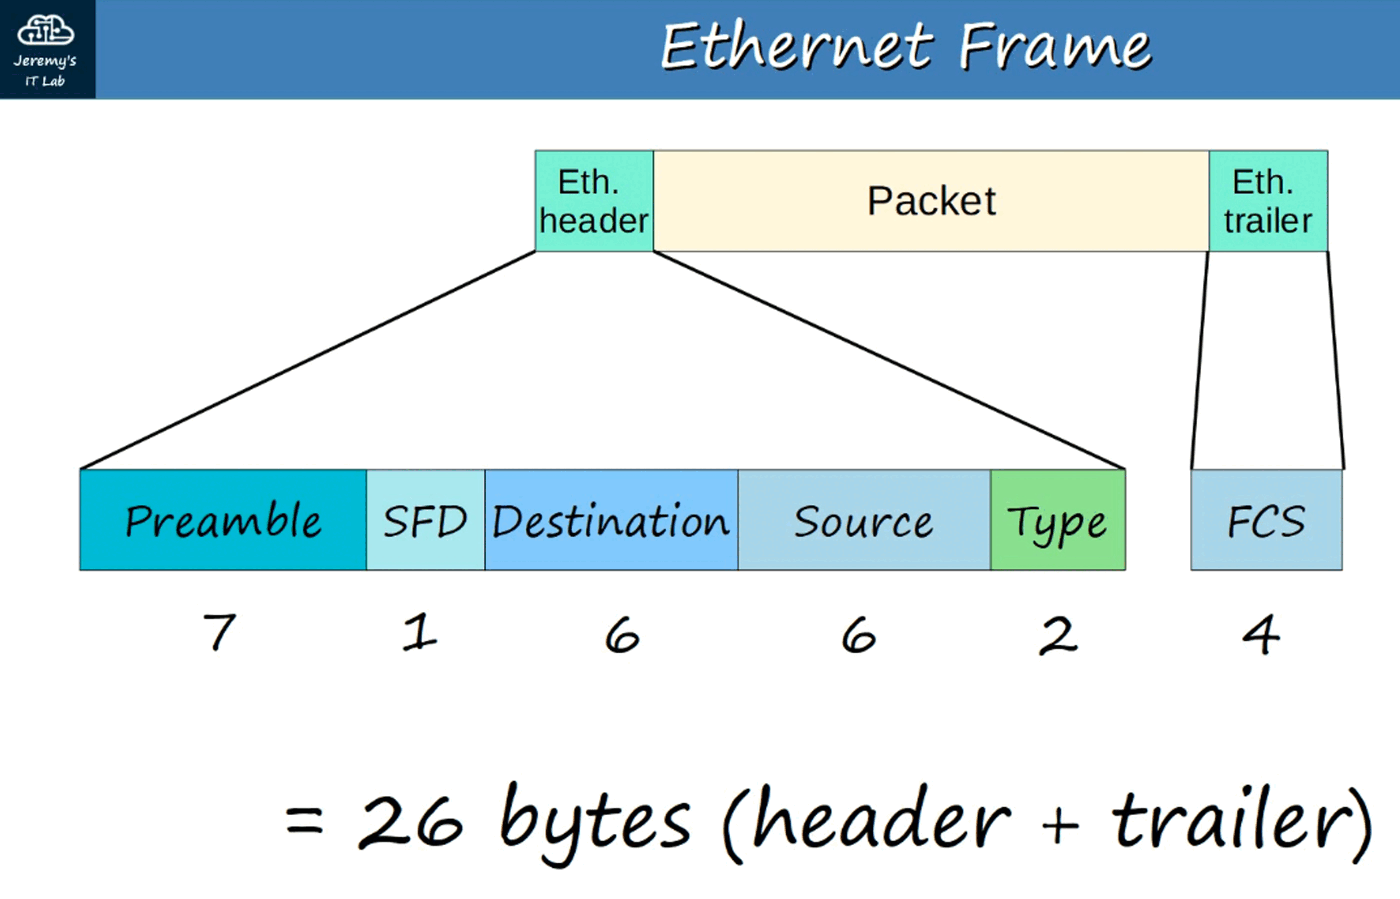
\includegraphics[keepaspectratio,alt={image}]{images/05-ethernet-lan-switching-part1/img-005.png}}
\end{figure}

MAC ADDRESS (48 bits long)

\begin{itemize}
\tightlist
\item
  6-bytes (48-bits) physical address assigned to the device when it is
  made.
\item
  AKA `Burned-In Address' (BIA)
\item
  Is globally unique
\item
  First 3 bytes are the OUI (Organizationally Unique Identifier) which
  is assigned to the company making the device
\item
  The last 3 bytes are unique to the device itself
\item
  Written as 12 hexadecimal characters
\end{itemize}

Example:

E8:BA:70 // 11:28:74 OUI // Unique Device ID

\section{Hexadecimal}\label{hexadecimal}

\begin{figure}
\centering
\pandocbounded{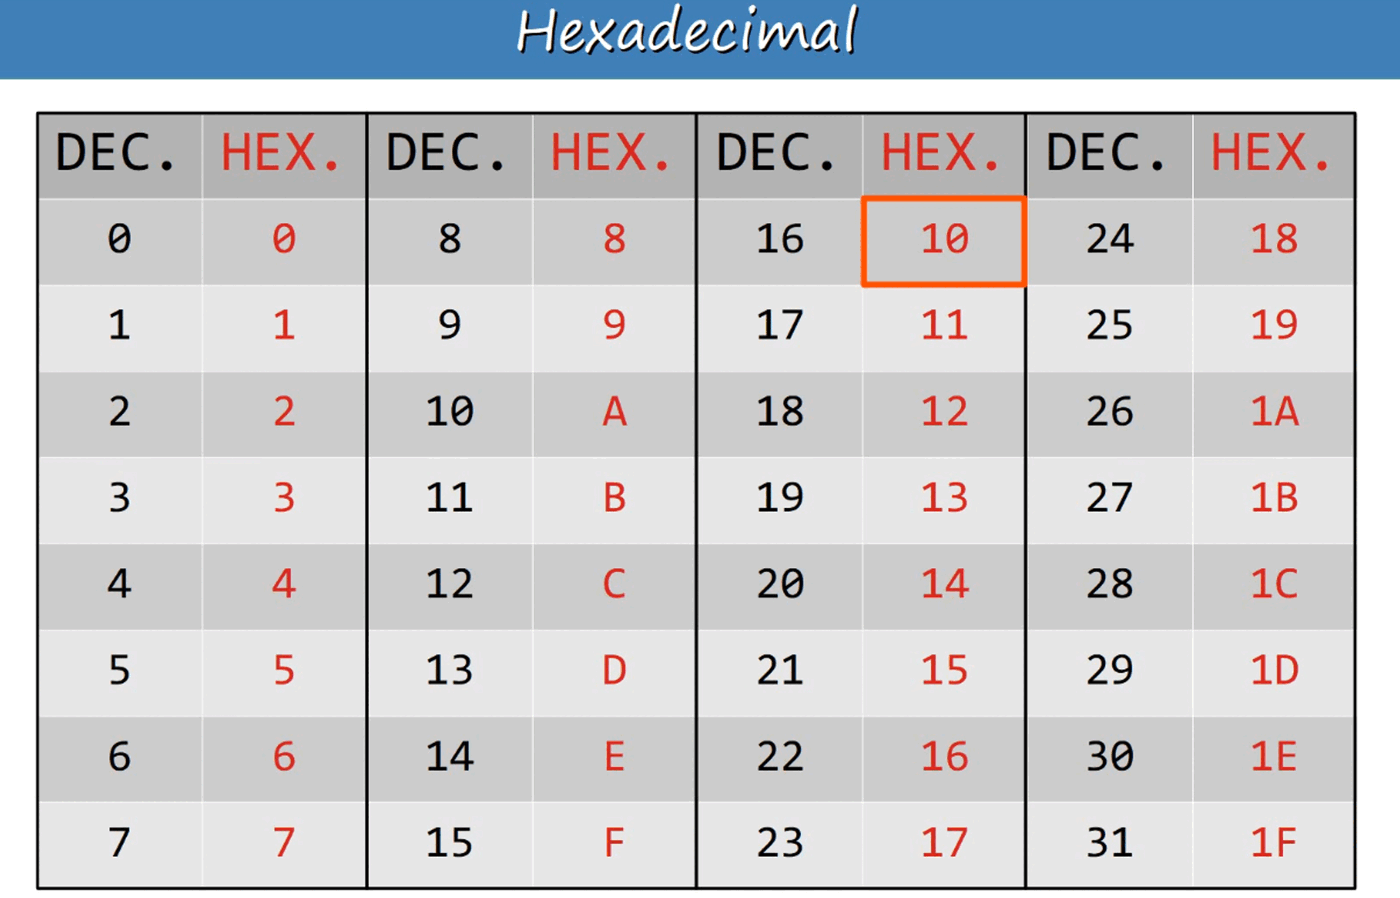
\includegraphics[keepaspectratio,alt={image}]{images/05-ethernet-lan-switching-part1/img-006.png}}
\end{figure}

\section{Interface Names}\label{interface-names}

F0/1, F0/2, F0/3\ldots{} F stands for ``Fast Ethernet'' or 100 Mbps
interfaces.

\section{MAC Address Table}\label{mac-address-table}

Each Switch stores a DYNAMICALLY LEARNED MAC ADDRESS TABLE, using the
SOURCE MAC ADDRESS of frames it receives.

\begin{figure}
\centering
\pandocbounded{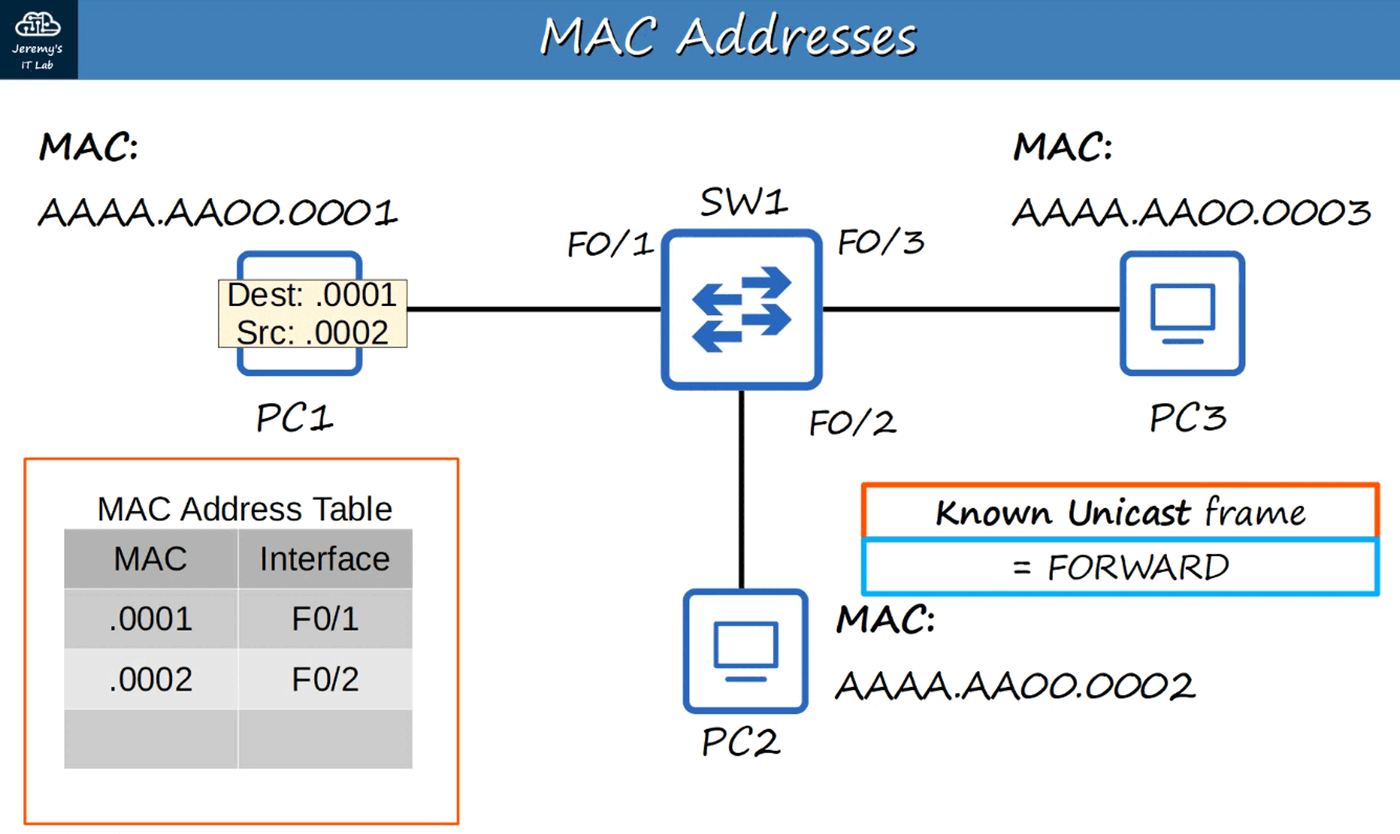
\includegraphics[keepaspectratio,alt={image}]{images/05-ethernet-lan-switching-part1/img-007.png}}
\end{figure}

When a Switch doesn't know the DESTINATION MAC ADDRESS of a frame
(UNKNOWN UNICAST FRAME), it is forced to FLOOD the frame - Forward the
frame out of ALL it's interfaces, except the one it received the packet
from.

When a KNOWN Unicast Frame is known (MAC Address is recognized by the
entry in the MAC ADDRESS TABLE), the frame is FORWARDED like normal.

\begin{figure}
\centering
\pandocbounded{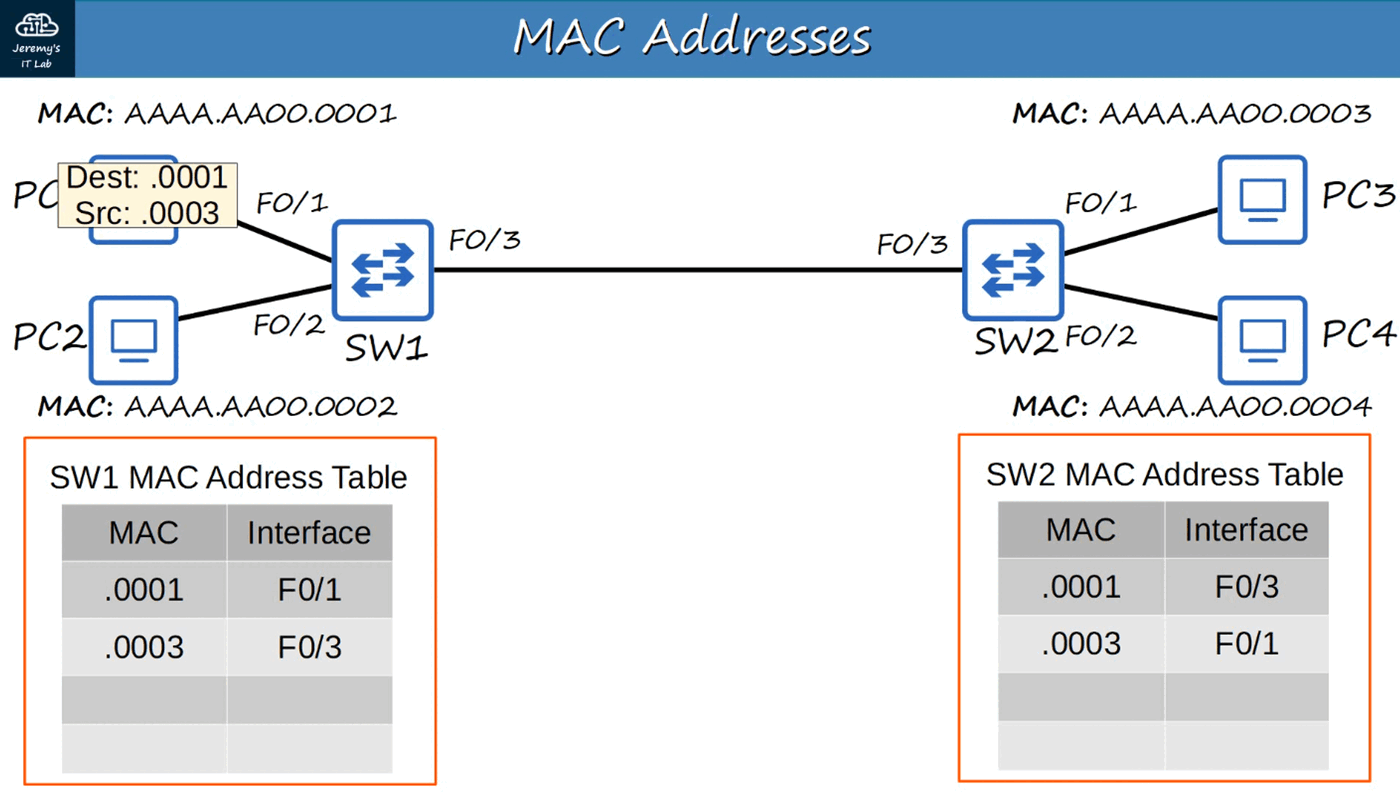
\includegraphics[keepaspectratio,alt={image}]{images/05-ethernet-lan-switching-part1/img-008.png}}
\end{figure}

\begin{itemize}
\tightlist
\item
  Note: Dynamic MAC Addresses are removed from the MAC ADDRESS TABLE
  every 5 minutes of inactivity.
\end{itemize}

\chapter{Ethernet LAN Switching: Part
2}\label{ethernet-lan-switching-part-2}

An ETHERNET FRAME looks like:

Ethernet Header --- DATA (Packet) --- Ethernet Trailer

\begin{figure}
\centering
\pandocbounded{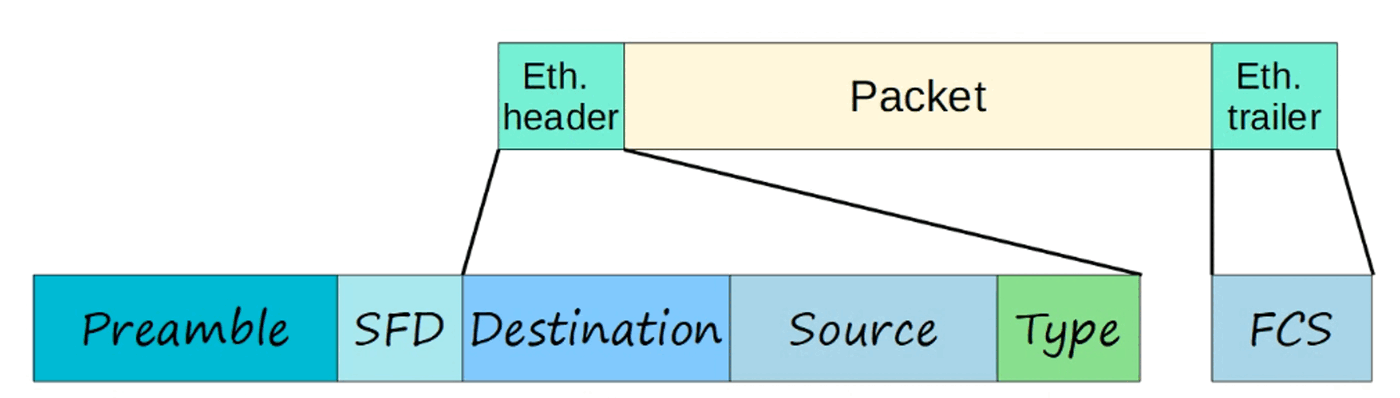
\includegraphics[keepaspectratio,alt={image}]{images/06-ethernet-lan-switching-part2/img-001.png}}
\end{figure}

The Ethernet Header contains 5 Fields:

Preamble -- SFD -- Destination -- Source -- Type/Length 7 bytes -- 1
byte -- 6 bytes -- 6 bytes -- 2 bytes

Ethernet Trailer contains 1 Field:

FCS (Frame Check Sequence) = 4 bytes

\begin{itemize}
\tightlist
\item
  The PREAMBLE + SFD is not usually considered part of the ETHERNET
  HEADER.
\end{itemize}

THEREFORE the size of the ETHERNET HEADER + TRAILER is 18 bytes

(6 + 6 + 2 + 4 bytes for the FRAME CHECK SEQUENCE)

The MINIMUM size for an ETHERNET FRAME (Header + Payload {[}PACKET{]} +
Trailer) is 64 BYTES.

64 BYTES - 18 BYTES (Header + Trailer size) = 46 BYTES

THEREFORE the MINIMUM DATA PAYLOAD (PACKET) size is 46 BYTES!

IF the PAYLOAD is LESS than 46 BYTES then PADDING BYTES are added
(padding bytes are a series of 0's) until it equals to 46 BYTES.

When a PC wants to send a packet to a destination, with a known IP
address but an unknown MAC address, it first needs to send an ARP
Request to learn that destination's MAC address.

\begin{figure}
\centering
\pandocbounded{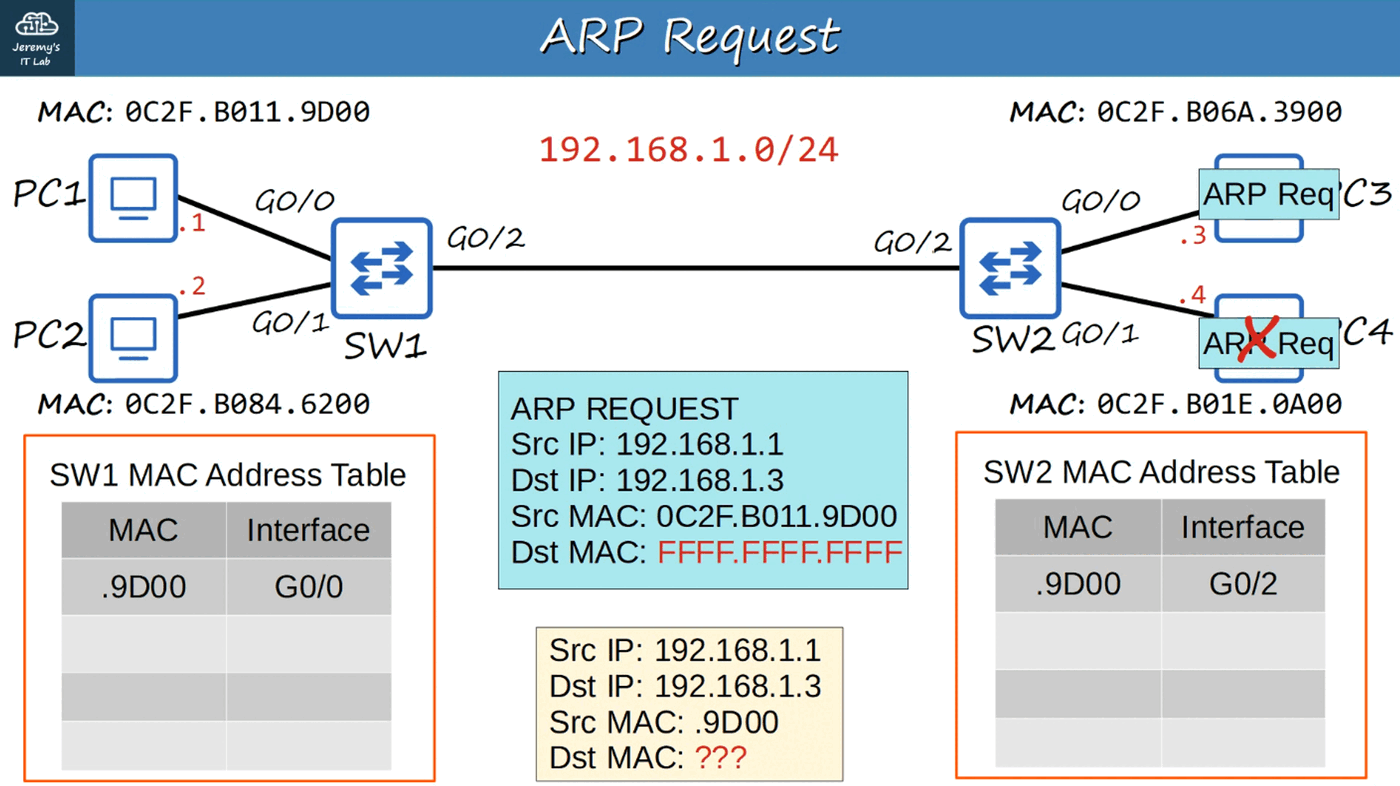
\includegraphics[keepaspectratio,alt={image}]{images/06-ethernet-lan-switching-part2/img-002.png}}
\end{figure}

\begin{itemize}
\tightlist
\item
  ARP stands for `Address Resolution Protocol'.
\item
  It is used to discover the Layer 2 address (MAC address) of a known
  Layer 3 address (IP address)
\item
  Consists of two messages:

  \begin{itemize}
  \tightlist
  \item
    ARP REQUEST (Source message)
  \item
    ARP REPLY (Destination message)
  \end{itemize}
\item
  ARP REQUEST is BROADCAST = sent to all hosts on network, except the
  one it received the request from.
\end{itemize}

An ARP REQUEST frame has:

\begin{itemize}
\tightlist
\item
  Source IP Address
\item
  Destination IP Address
\item
  Source MAC address
\item
  BROADCAST MAC Address - FFFF.FFFF.FFFF
\end{itemize}

An ARP REPLY frame has:

\begin{itemize}
\tightlist
\item
  Source IP Address
\item
  Destination IP Address
\item
  Source MAC address
\item
  Destination MAC Address
\end{itemize}

ARP REPLY is a known UNICAST frame = Sent only to the host that sent the
ARP REQUEST.

\begin{figure}
\centering
\pandocbounded{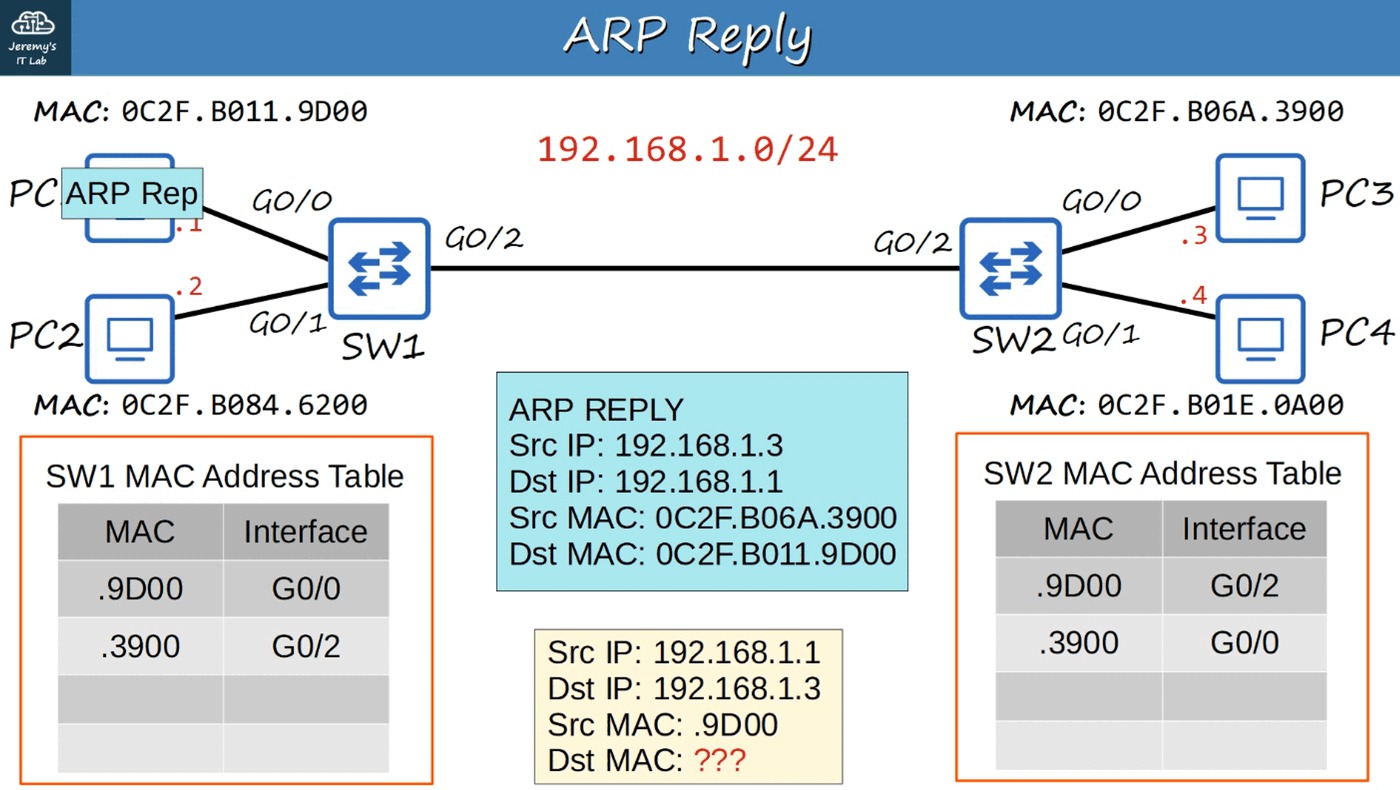
\includegraphics[keepaspectratio,alt={image}]{images/06-ethernet-lan-switching-part2/img-003.png}}
\end{figure}

\section{Ping}\label{ping}

\begin{itemize}
\tightlist
\item
  A network utility that is used to test reachability
\item
  Measures round-trip time
\item
  Uses two messages:

  \begin{itemize}
  \tightlist
  \item
    ICMP Echo REQUEST
  \item
    ICMP Echo REPLY
  \end{itemize}
\item
  Is UNICAST
\item
  Command to use ping:

  \begin{itemize}
  \tightlist
  \item
    ping \textless ip-address\textgreater{}
  \end{itemize}
\end{itemize}

By Default, a CISCO IOS sends 5 ICMP requests/replies (Default size is
100-bytes)

\begin{itemize}
\tightlist
\item
  A period (.) is a failed ping
\item
  An exclamation mark (!) is a successful ping
\end{itemize}

USEFUL CISCO IOS COMMANDS (from Privileged EXEC mode)

PC1\# show arp // shows hosts ARP table

\begin{figure}
\centering
\pandocbounded{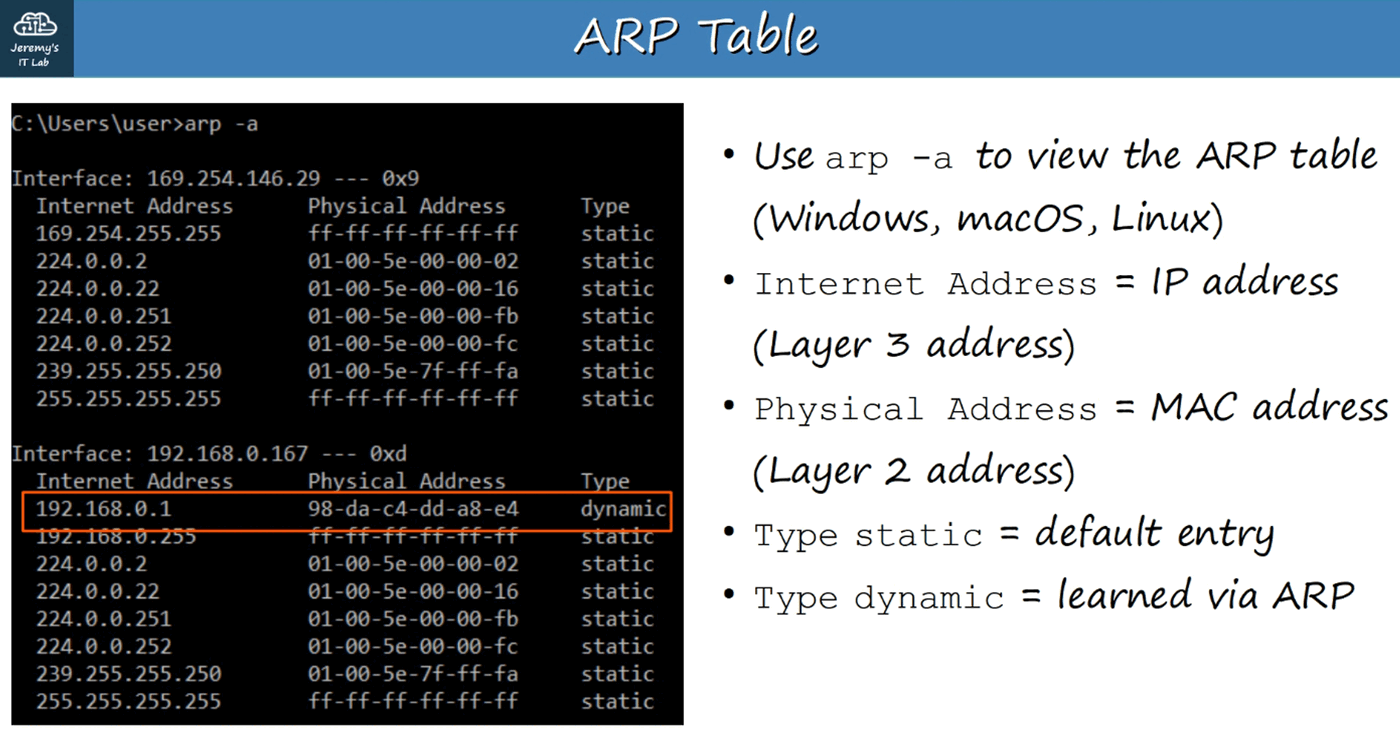
\includegraphics[keepaspectratio,alt={image}]{images/06-ethernet-lan-switching-part2/img-004.png}}
\end{figure}

SW1\#show mac address-table // show the switches MAC table

\begin{figure}
\centering
\pandocbounded{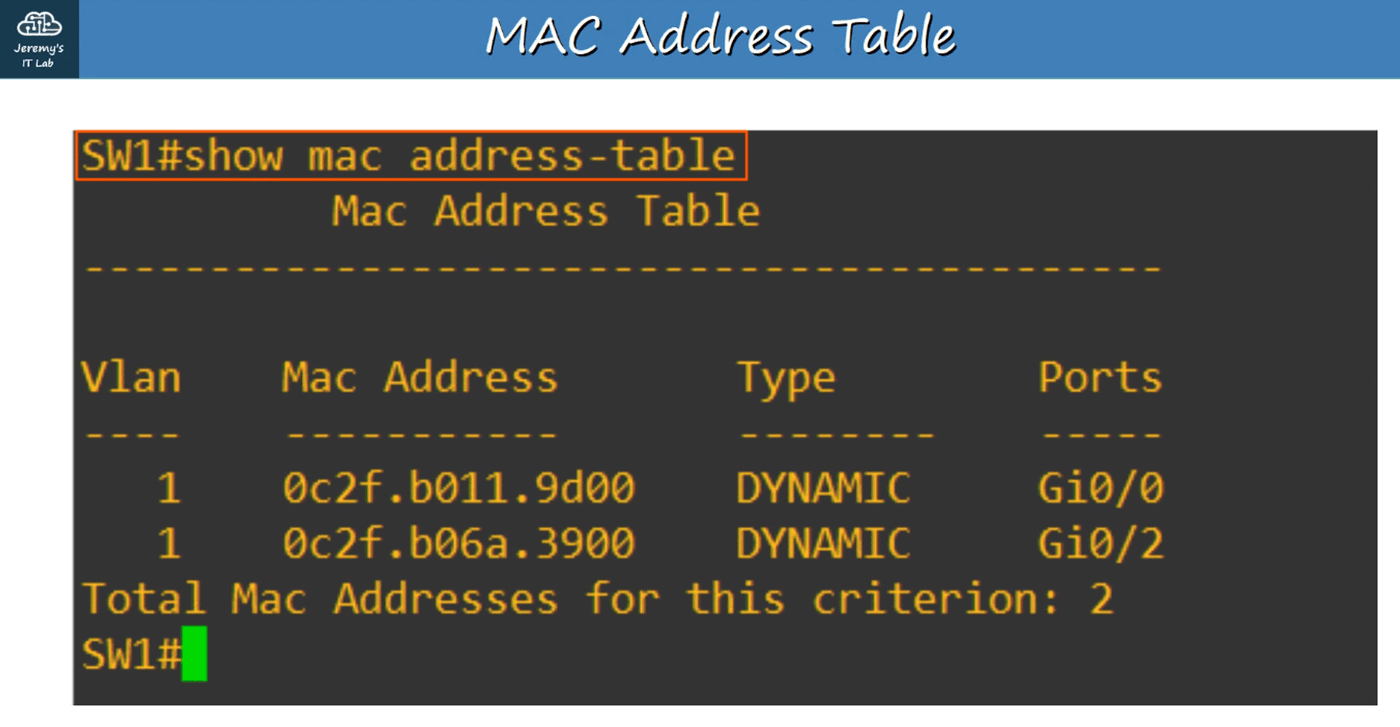
\includegraphics[keepaspectratio,alt={image}]{images/06-ethernet-lan-switching-part2/img-005.png}}
\end{figure}

Will show:

Vlan --- MAC Address --- Type --- Ports(interfaces)

(Vlan = Virtual Local Area Network)

\begin{figure}
\centering
\pandocbounded{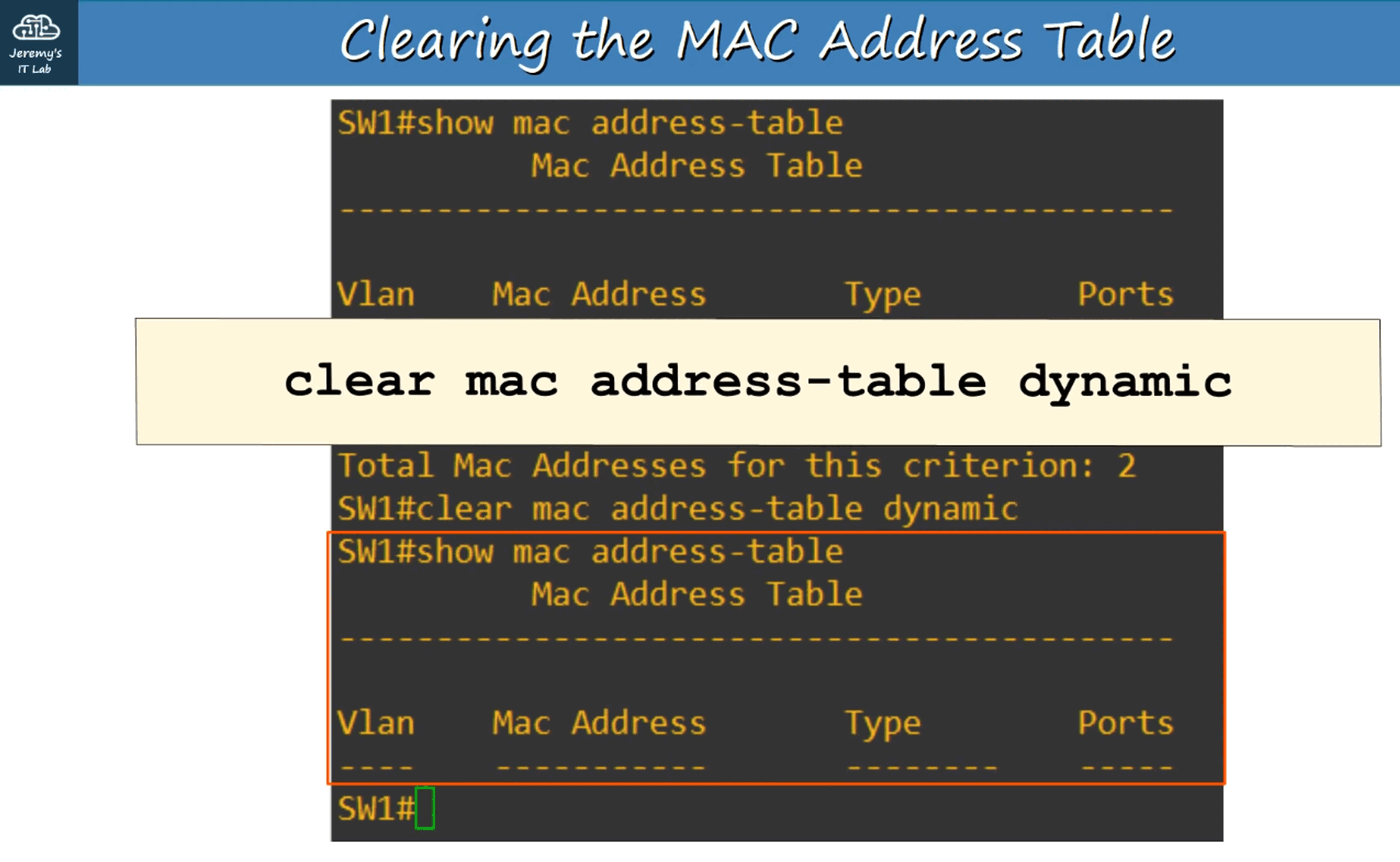
\includegraphics[keepaspectratio,alt={image}]{images/06-ethernet-lan-switching-part2/img-006.png}}
\end{figure}

SW1\# clear mac address-table dynamic \textless optional MAC
address\textgreater{}

// clears the entire switches MAC table. // IF the optional MAC address
is used, it will clear the SPECFIC MAC address.

SW1 \#clear mac address-table dynamic interface \textless optional
Interface\textgreater{}

// clears the MAC table entry of the Switch by it's \textbf{INTERFACE
n}ame.

\chapter{IPv4 Addressing: Part 1}\label{ipv4-addressing-part-1}

OSI MODEL - NETWORK LAYER (Layer 3)

\begin{itemize}
\tightlist
\item
  Provides connectivity between end hosts on DIFFERENT networks (ie:
  outside of the LAN)
\item
  Provides logical addressing (IP addresses)
\item
  Provides path selection between SOURCE and DESTINATION
\item
  ROUTERS operate at LAYER 3
\end{itemize}

\section{Routing}\label{routing}

SWITCHES (Layer 2 Devices) do no separate different networks. They
connect and EXPAND networks within the same LAN.

By adding a ROUTER, however, between two SWITCHES, you create a SPLIT in
the network; each with it's own network IP address.

Example: 192.168.1.0/24 (255.255.255.0) 192.168.2.0/24 (255.255.255.0)

\begin{figure}
\centering
\pandocbounded{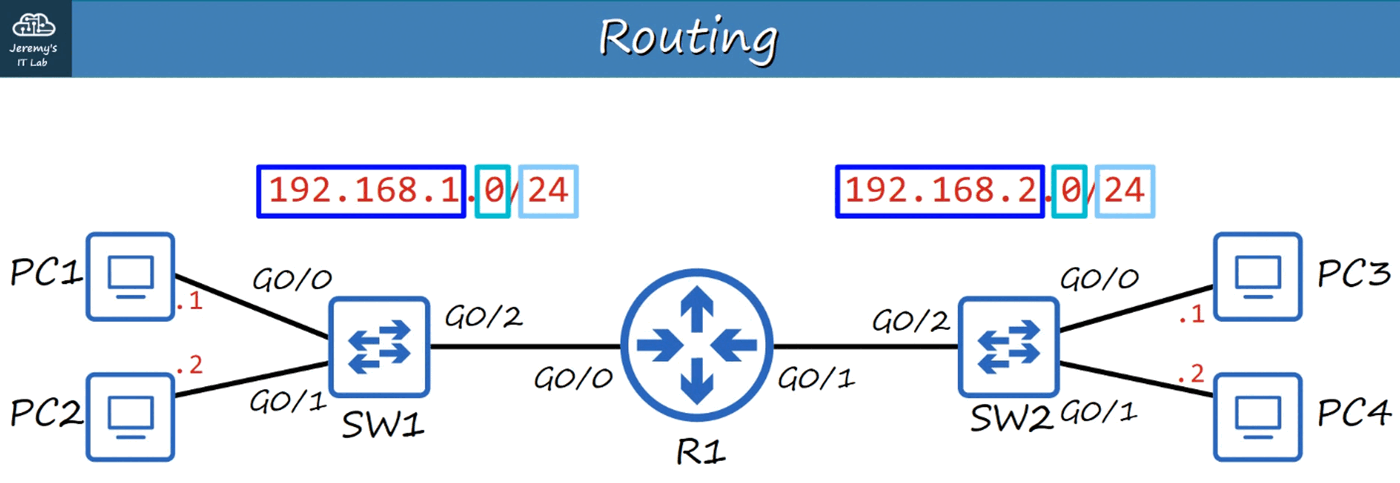
\includegraphics[keepaspectratio,alt={image}]{images/07-ipv4-addressing-part1/img-001.png}}
\end{figure}

ROUTERS have unique IP Addresses for EACH of their interface
connections, depending on their location.

The IP Address for the ROUTER's G0/0 Interface is: 192.168.1.254/24

The IP Address for the ROUTER's G0/1 Interface is: 192.168.2.254/24

\begin{figure}
\centering
\pandocbounded{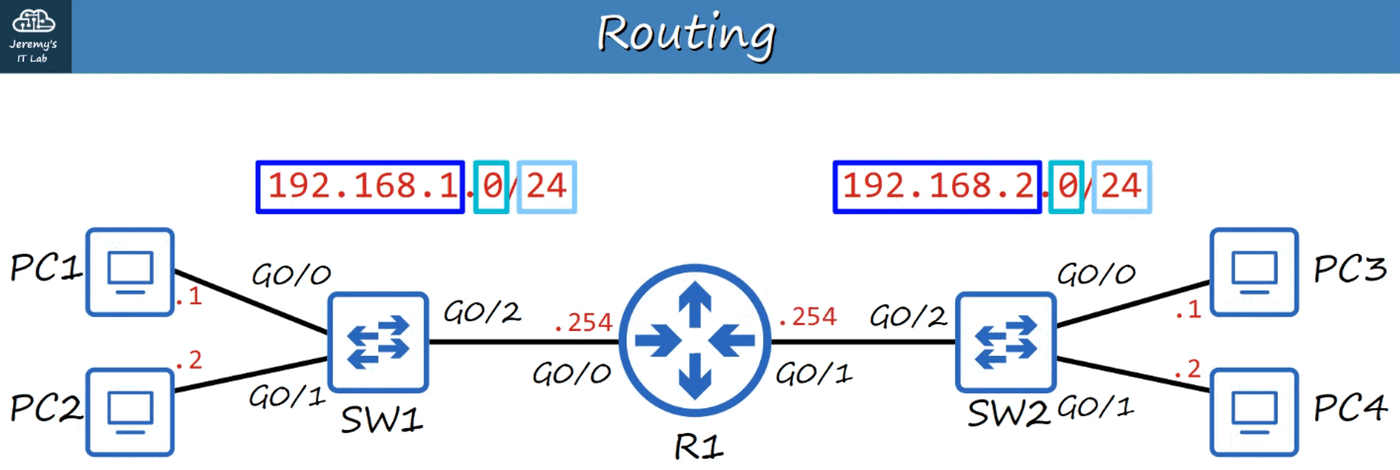
\includegraphics[keepaspectratio,alt={image}]{images/07-ipv4-addressing-part1/img-002.png}}
\end{figure}

The IP Address depends on network address of the LAN it is connects to.

The NETWORK portion of given IP Address will be the same for all HOSTS
on a given LAN.

Example:

192.168.1.100 192.168.1.105 192.168.1.205

All of these addresses are on the SAME Network because the NETWORK
PORTION of their IP Address is the same (192.168.1) while the HOST part
(100,105,205) is UNIQUE!

When a BROADCAST message hits a ROUTER, it does NOT continue onward. It
stays within the LOCAL LAN (Switch/Hosts).

IPv4 HEADER

\begin{figure}
\centering
\pandocbounded{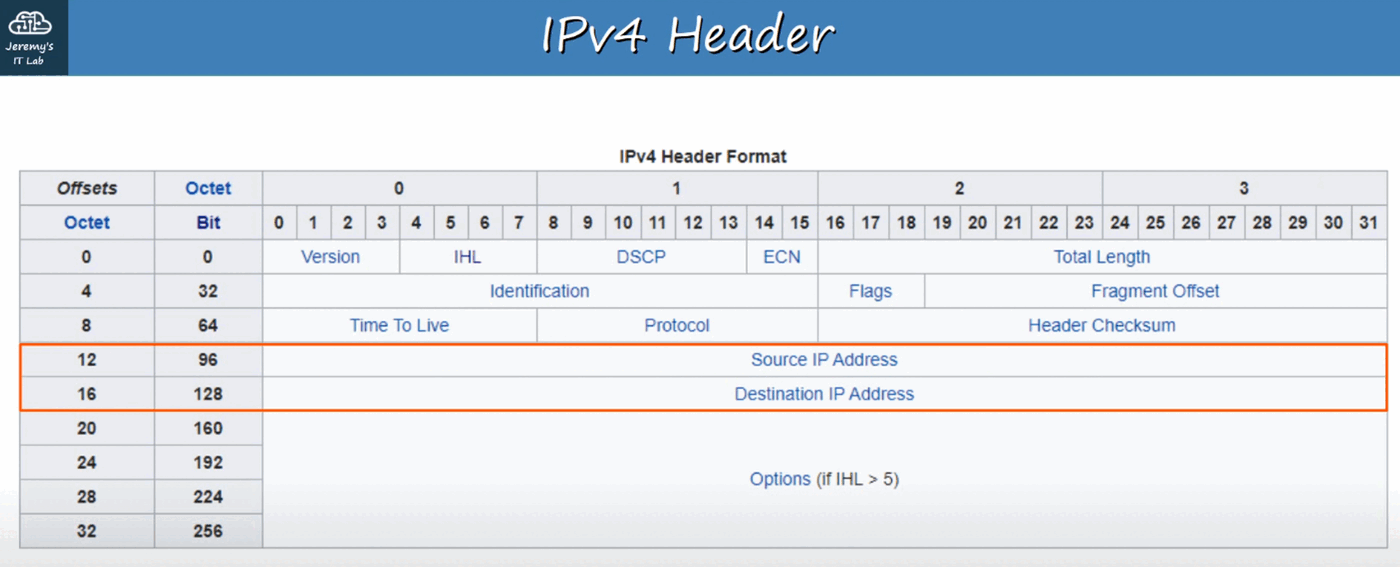
\includegraphics[keepaspectratio,alt={image}]{images/07-ipv4-addressing-part1/img-003.png}}
\end{figure}

IP (or Internet Protocol) is the primary Layer 3 protocol in use today.
Version 4 is the version in use in most networks.

IPv4 Headers contain MORE fields than the ETHERNET header.

IPv4 Headers contain a SOURCE IP Address and DESTINATION IP Address
field.

This FIELD is 32-bits(4-bytes) in length (0-31)

192.168.1.254 (each decimal number represents 8 bits)

Translated to Binary:

11000000 . 10101000 . 00000001 . 11111110

EACH of these 8 bit groups are referred to as an OCTET

Since Binary is difficult to read for people, we use the Dotted Decimal
format.

REVIEW of DECIMAL and HEXADECIMAL

\begin{figure}
\centering
\pandocbounded{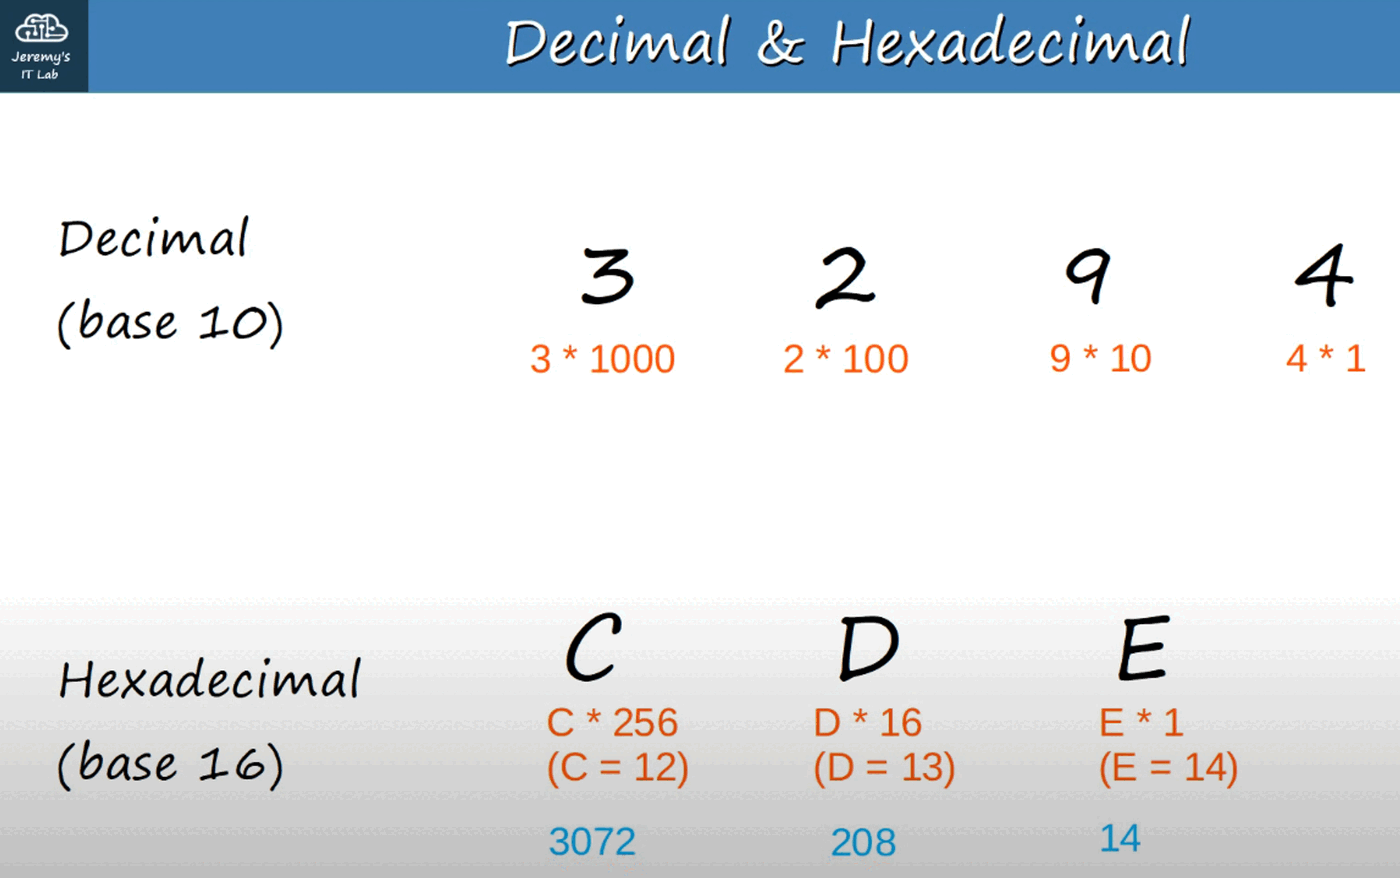
\includegraphics[keepaspectratio,alt={image}]{images/07-ipv4-addressing-part1/img-004.png}}
\end{figure}

Decimal (base 10)

Ex: 3294 = (3 * 1000) + (2 * 100) + (9 * 10) + (4 * 1)

Hexadecimal (base 16)

Ex: 3294, would be CDE

\begin{lstlisting}
C (C * 256 / 12 * 256 = 3072) // 256ths position
D (D * 16 / D=13 so 16*13 = 208) // 16ths position
E (E * 1 / E = 14)  // 1s position
\end{lstlisting}

Adding these up, we get 3294

So, how do we convert a BINARY NUMBER to a DECIMAL NUMBER? The same way
we convert to Hexadecimal.

10001111

So:

\begin{lstlisting}
1 * 128 = 128
1 * 8 = 8
1 * 4 = 4
1 * 2 = 2
1 * 1 = 1
\end{lstlisting}

Add them all up : 128 + 8 + 4 + 2 + 1 = 143

The answer is 143.

Another example:

01110110

\begin{lstlisting}
1 * 64 = 64
1 * 32 = 32
1 * 16 = 16
1 * 4 = 4
1 * 2 = 2
\end{lstlisting}

Add them all up: 64 + 32 + 16 + 4 + 2 = 118

The answer is 118.

Another example:

11101100

\begin{lstlisting}
1 * 128 = 128
1 * 64 = 64
1 * 32 = 32
1 * 8 = 8
1 * 4 = 4
\end{lstlisting}

Add them all up: 128 + 64 + 32 + 8 + 4 = 236

The answer is 236.

So, how do we convert a DECIMAL NUMBER to a BINARY NUMBER?

Take the number 221.

We can take that number and start subtracting it from LEFT to RIGHT of
our Binary slots.

221

\begin{lstlisting}
221 - 128 = 93 so we place a 1 in the "128" slot
\end{lstlisting}

10000000

\begin{lstlisting}
93 - 64 = 29 so we place another 1 in the "64" slot

29 - 32 isn't possible so we place a 0 in the "32" slot

29 - 16 = 13 so we place a 1 in the "16" slot

13 - 8 = 5 so we place a 1 in the "8" slot

5 - 4 = 1 so we place a 1 in the "4" slot

1 - 2 isn't possible so we put a 0 in the "2" slot

1 - 1 is possible so we put a 1 in the "1" slot
\end{lstlisting}

This, then, allows us to the write out the BINARY number for 221.

It is : 11011101

Another example: 127

\begin{lstlisting}
127 - 128 is not possible so 0 in "128"
127 - 64 is possible so 1 in "64"
63 - 32 is possible so 1 in "32"
31 - 16 is possible so 1 in "16"
15 - 8 is possible so 1 in "8"
7 - 4 is possible so 1 in "4"
3 - 2 is possible so 1 in "2"
1 is possible so 1 in "1"
\end{lstlisting}

So 127, in BINARY, is 0111 1111

Another example: 207

Alternatively, you can subtract the number from `255' (which is
1111111). The remainder, then, can be used to ``find'' where the 0's are
in the binary number.

255 - 207 = 48 so \ldots{}

1 1 0 0 1 1 1 1 (32 + 16 = 48)

11001111 is the correct answer.

IPv4 ADDRESSES

So we now know that IP Addresses are the Dotted Decimal conversion of a
series of BINARY NUMBERS (broken up into 4 OCTETS) like so:

192.168.1.254/24

But what does the /24 stand for?

\begin{figure}
\centering
\pandocbounded{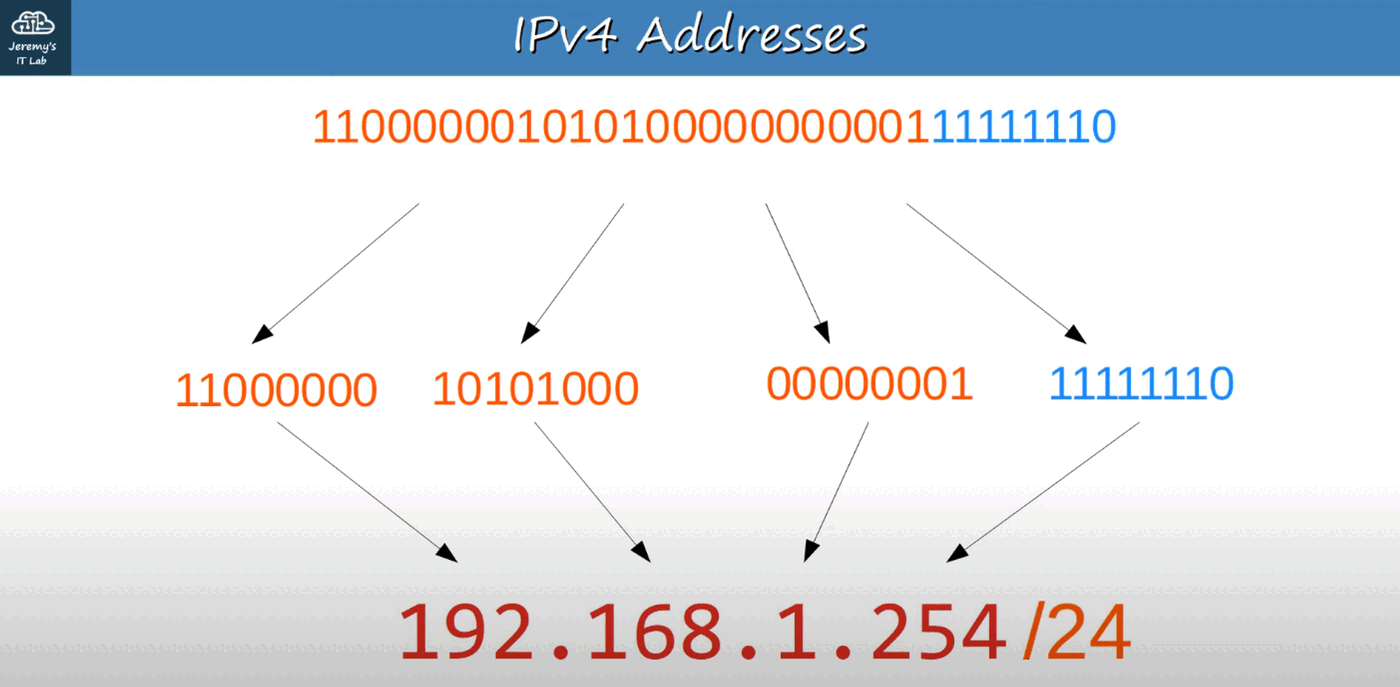
\includegraphics[keepaspectratio,alt={image}]{images/07-ipv4-addressing-part1/img-005.png}}
\end{figure}

It means the FIRST 24 BITS of this address represent the NETWORK portion
of the address.

192.168.1 is the NETWORK PORTION (the first 3 OCTETS)

.254 is the HOST PORTION (the last OCTET)

\begin{figure}
\centering
\pandocbounded{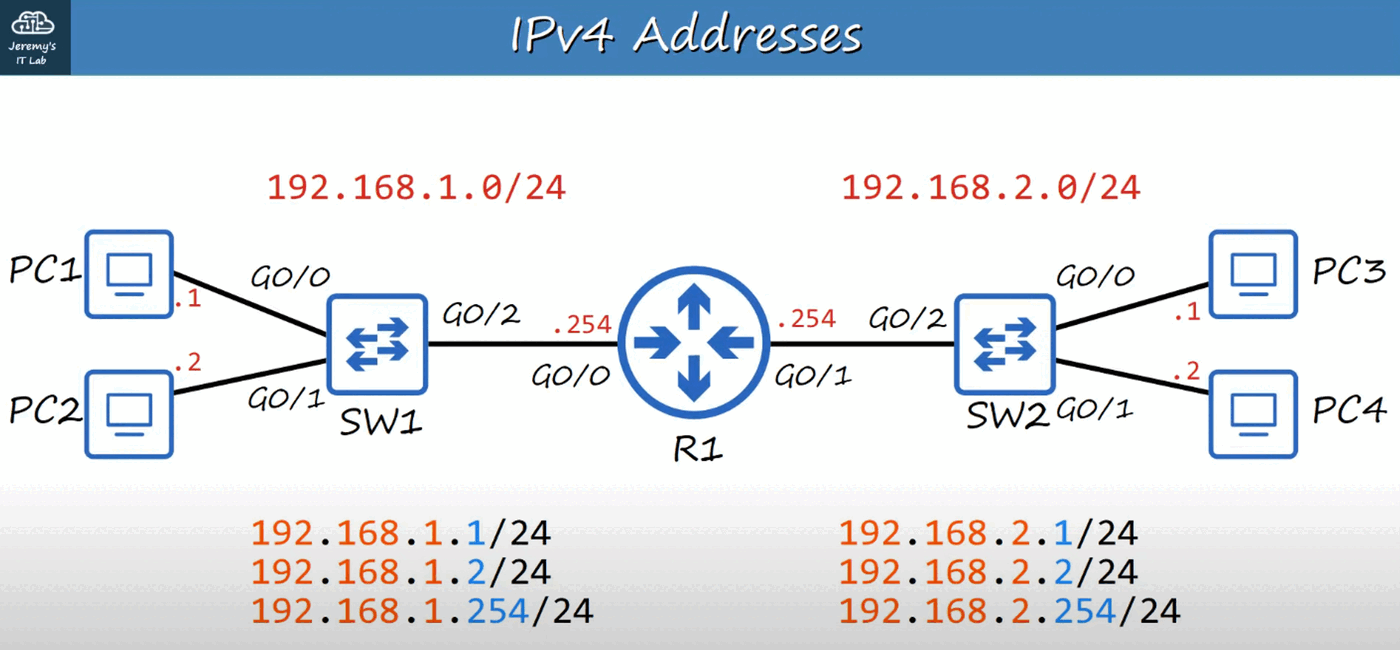
\includegraphics[keepaspectratio,alt={image}]{images/07-ipv4-addressing-part1/img-006.png}}
\end{figure}

CONVERT this BINARY number into an IPv4 Address:

10011010010011100110111100100000

10011010 . 01001110 . 01101111 . 00100000

Octets:

\begin{enumerate}
\def\labelenumi{\arabic{enumi}.}
\tightlist
\item
  128 + 16 + 8 + 2 = 154
\item
  64 + 8 + 4 + 2 = 78
\item
  64 + 32 + 8 + 4 + 2 + 1 = 111
\item
  32
\end{enumerate}

The IPv4 address is: 154.78.111.32/16

154.78 is the NETWORK PORTION 111.32 is the HOST PORTION

Another Example:

00001100100000001111101100010111

00001100 . 10000000 . 11111011 . 00010111

Octets:

\begin{enumerate}
\def\labelenumi{\arabic{enumi}.}
\tightlist
\item
  8 + 4 = 12
\item
  128
\item
  255 - 4 = 251
\item
  16 + 4 + 2 + 1 = 23
\end{enumerate}

The IPv4 address is: 12.128.251.23/8

12 is the NETWORK PORTION 128.251.23 is the HOST PORTION

IPv4 ADDRESS CLASSES

IPv4 ADDRESSES are split up into 5 different `classes'. The class of an
IPv4 is determined by the FIRST OCTET of the address.

\begin{lstlisting}
CLASS       FIRST OCTET         FIRST OCTET NUMBERIC RANGE

A            0xxxxxxx               0-126 + 127 'loopback'
B            10xxxxxx               128-191
C            110xxxxx               192-223
D            1110xxxx               224-239
E            1111xxxx               240-255
\end{lstlisting}

From the above chart, if the FIRST OCTECT STARTS with 0, the numeric
RANGE of possible first DOTTED DECIMAL is between 0-127.

The CLASSES we will be focusing on are CLASS A to CLASS C.

\begin{figure}
\centering
\pandocbounded{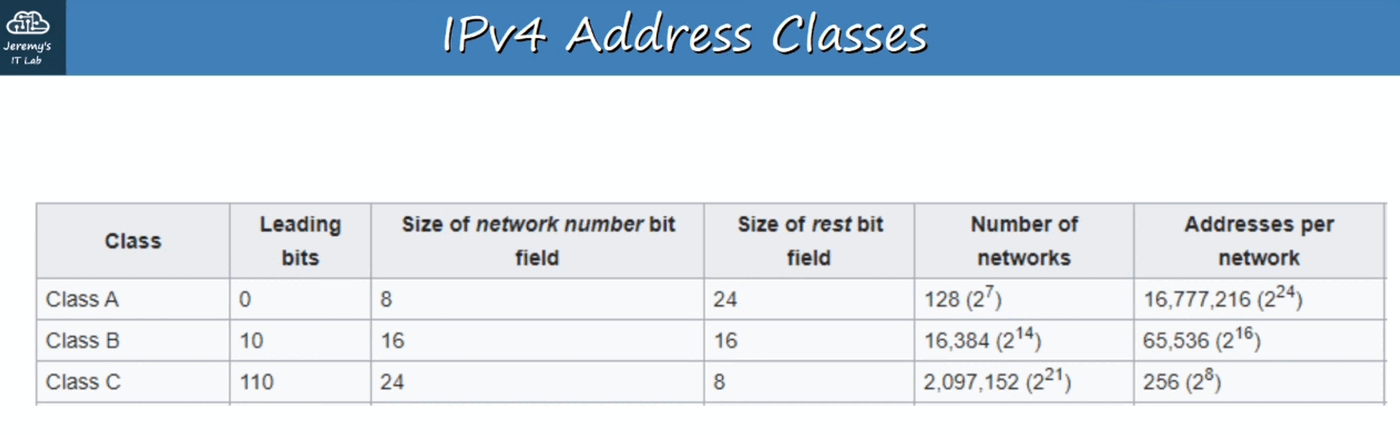
\includegraphics[keepaspectratio,alt={image}]{images/07-ipv4-addressing-part1/img-007.png}}
\end{figure}

D CLASS are reserved for `MULTICAST' ADDRESSES

E CLASS are reserved for `EXPERIMENTAL' ADDRESSES

A CLASS USUALLY have a range of 1-126? WHY?

Because 127 is usually reserved for `loopback addresses'

127.0.0.0 to 127.255.255.255 are used to test the network.

\begin{itemize}
\tightlist
\item
  Used to test the `Network stack' (OSI \& TCP/IP model) on the local
  device.
\end{itemize}

\begin{figure}
\centering
\pandocbounded{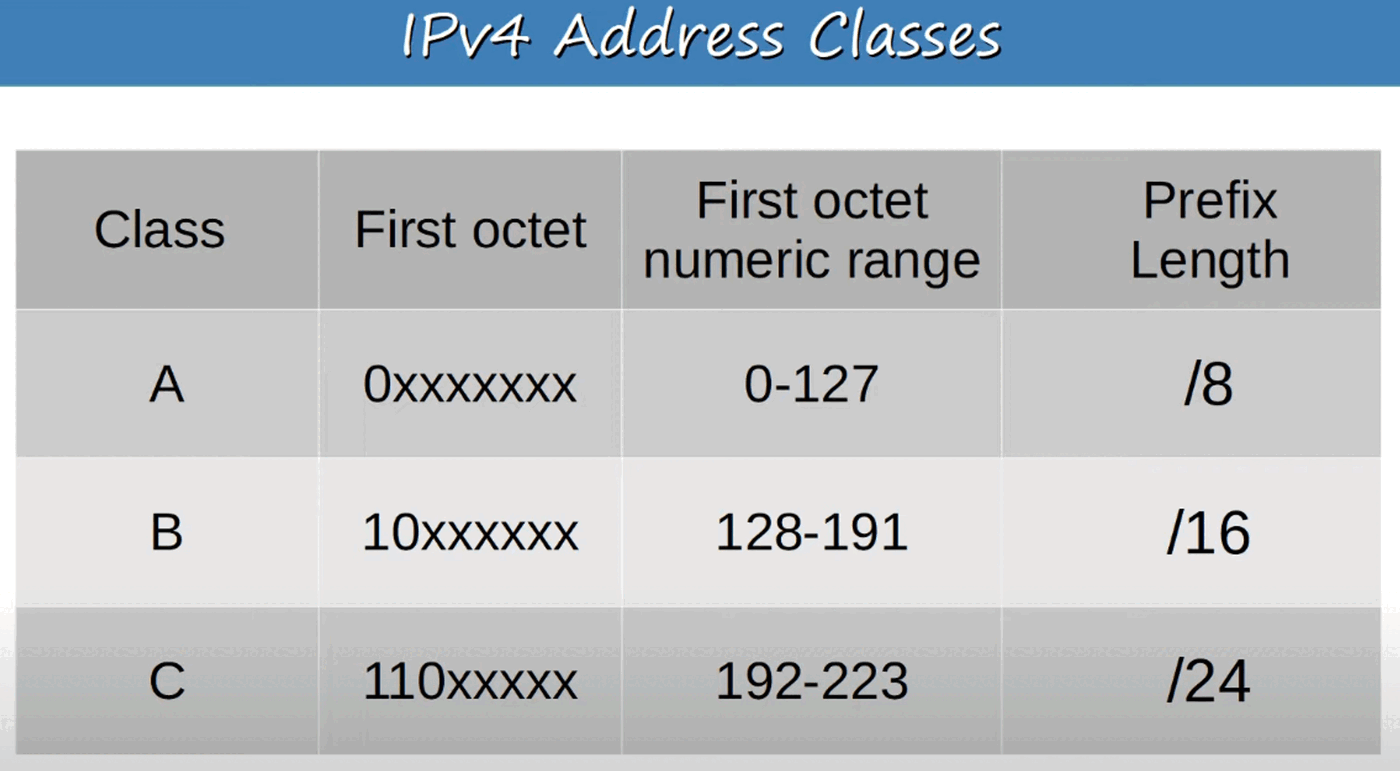
\includegraphics[keepaspectratio,alt={image}]{images/07-ipv4-addressing-part1/img-008.png}}
\end{figure}

The PREFIX LENGTH is the LENGTH of the NETWORK PORTION of the Address.

From the examples above:

12.128.251.23/8 is a CLASS A Address 154.78.111.32/16 is a CLASS B
Address 192.168.1.254/24 is a CLASS C Address

Because the NETWORK portion of CLASS A is so short, it means there are a
LOT more potential Hosts.

Because the NETWORK portion of CLASS C is so long, it means fewer
potential Hosts.

\section{Netmask}\label{netmask}

\begin{figure}
\centering
\pandocbounded{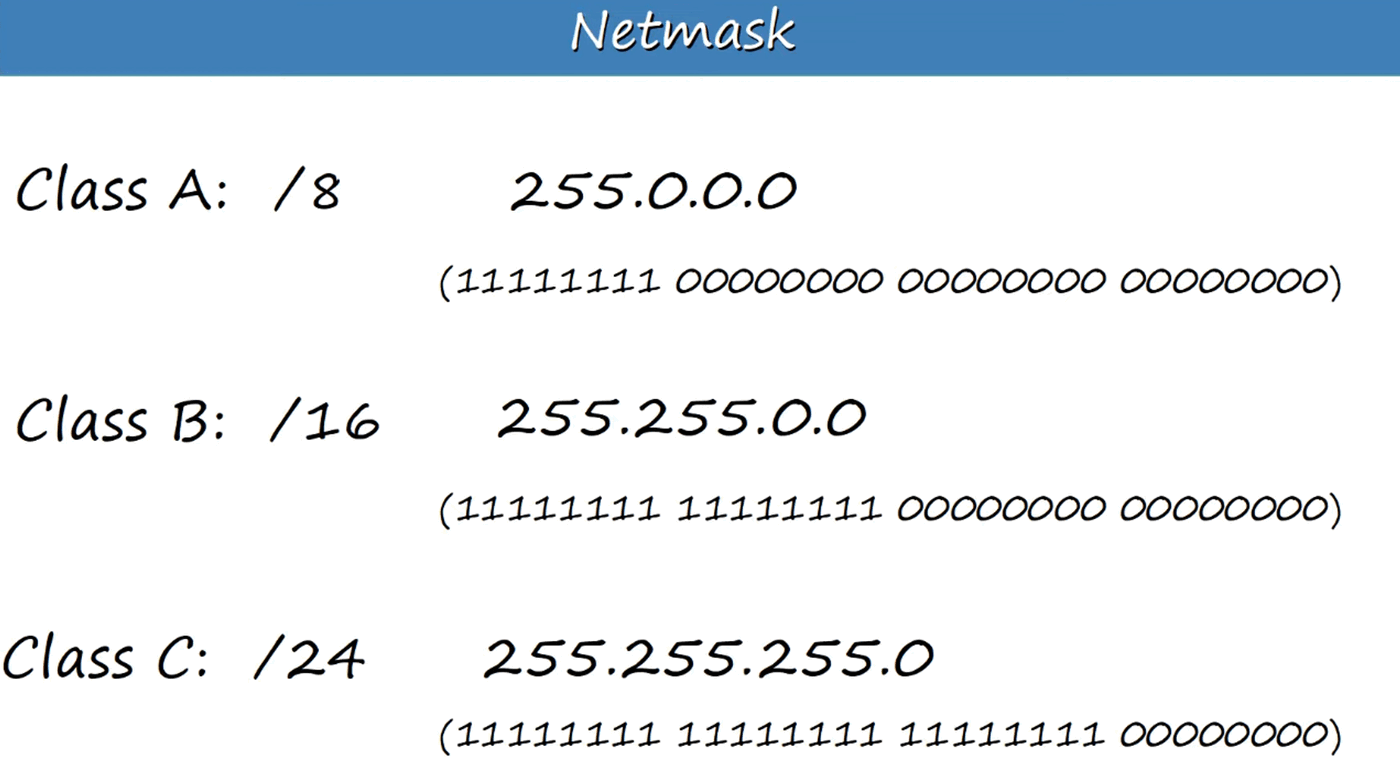
\includegraphics[keepaspectratio,alt={image}]{images/07-ipv4-addressing-part1/img-009.png}}
\end{figure}

A NETMASK is written like a Dotted Decimal IP Address

CLASS A: /8 = 255.0.0.0

CLASS B: / 16 = 255.255.0.0

CLASS C: /24 = 255.255.255.0

\section{Network Addresses}\label{network-addresses}

\begin{figure}
\centering
\pandocbounded{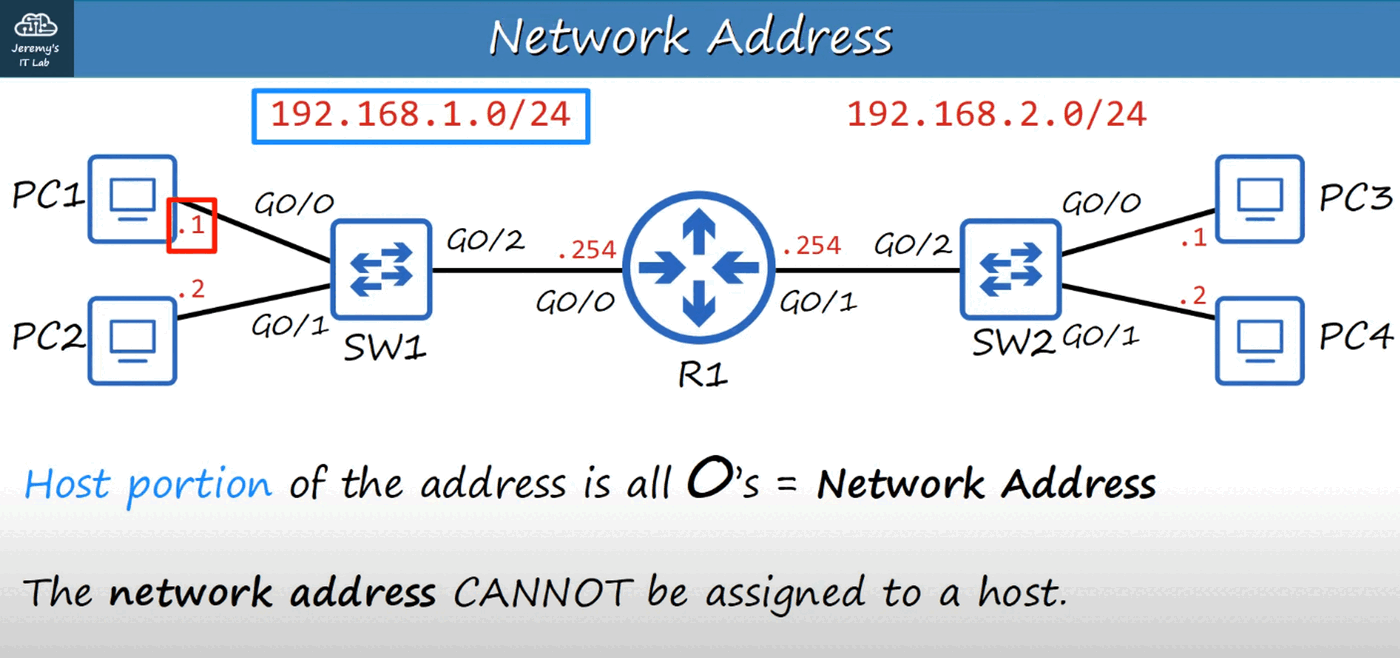
\includegraphics[keepaspectratio,alt={image}]{images/07-ipv4-addressing-part1/img-010.png}}
\end{figure}

If the HOST PORTION of an IP ADDRESS is ALL 0's, it means it is the
NETWORK ADDRESS = the identifier of the network itself.

Example: 192.168.1.0/24 = THIS is a NETWORK ADDRESS.

A NETWORK ADDRESS cannot be assigned to a HOST. A NETWORK ADDRESS is the
FIRST ADDRESS.

\begin{figure}
\centering
\pandocbounded{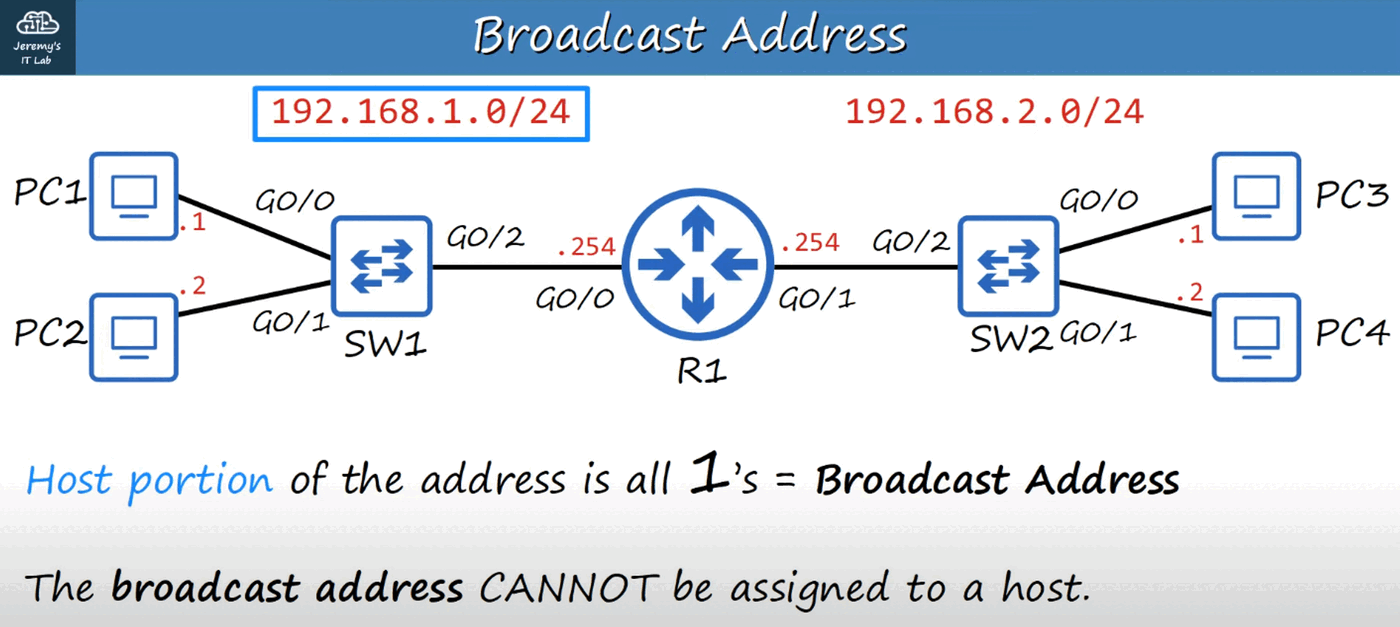
\includegraphics[keepaspectratio,alt={image}]{images/07-ipv4-addressing-part1/img-011.png}}
\end{figure}

If the HOST PORTION of an IP ADDRESS is ALL 1's, it means it is the
BROADCAST ADDRESS for the network.

A BROADCAST ADDRESS cannot be assigned to a HOST.

DESTINATION IP : 192.168.1.255 (Broadcast IP address) DESTINATION MAC :
FFFF.FFFF.FFFF (Broadcast MAC address)

Because of the two `reserved' addresses, the range of USABLE HOST
ADDRESSES is 1 to 254.

\chapter{IPv4 Addressing: Part 2}\label{ipv4-addressing-part-2}

\section{Maximum Hosts per Network}\label{maximum-hosts-per-network}

Let's take a Class C Network:

192.168.1.0/24

(gives a range of 0 ---\textgreater{} 255)

Said another way, the HOST portion (the .0) is equal to 8 bits
so\ldots{}

Host portion = 8 bits = 2\^{}8 = 256

HOWEVER, since the Network Address (Network ID)

192.168.1.0 is Reserved

AND

192.168.1.255 (BROADCAST ADDRESS) is ALSO reserved.

The MAXIMUM Hosts per Network = 2\^{}8-2 = 254 hosts

What about a Class B Network ?

172.16.0.0/16 ----\textgreater{} 172.16.255.255/16

Host portion = 16 bits = 2\^{}16 = 65,536

Maximum hosts per network = 2\^{}16-2 = 65,534 hosts

What about a Class A Network ?

10.0.0.0/8 -------------\textgreater{} 10.255.255.255/8

Host portion = 24 bits = 2\^{}24 = 16,777,216

Maximum hosts per network = 2\^{}24-2 = 16,777,214 hosts

\section{Therefore}\label{therefore}

The formula for calculating the number of HOSTS on a network is:

2 \^{} N - 2 (2 to the power of N - 2)

where N = number of HOST bits

\section{First / Last Usable
Addresses}\label{first-last-usable-addresses}

Class C Network

192.168.1.0/24 (NETWORK ADDRESS)

Add 1 so the Host Portion = 00000001

192.168.1.1/24 = FIRST USABLE ADDRESS

192.168.1.255/24 (BROADCAST ADDRESS)

Subtract 1 from the BROADCAST ADDRESS = 11111110

192.168.1.254/24 = LAST USABLE ADDRESS

Class B Network

172.16.0.0/16 (NETWORK ADDRESS)

Add 1 to Host portion so 0000 0000 0000 0001

172.16.0.1/16 is the FIRST USABLE ADDRESS

172.16.255.255/16 (BROADCAST ADDRESS)

Subtract 1 to Broadcast Address so 1111 1111 1111 1110

172.16.255.254/16 is the LAST USABLE ADDRESS

Class A Network

10.0.0.0/8 (NETWORK ADDRESS)

Add 1 to Host portion so 00000000 00000000 00000001

10.0.0.1/8 is the FIRST USABLE ADDRESS

10.255.255.255/8 (BROADCAST ADDRESS)

Subtract 1 to Broadcast Address so 1111 1111 1111 1110

10.255.255.254/16 is the LAST USABLE ADDRESS

\section{Cisco CLI Device
Configuration}\label{cisco-cli-device-configuration}

R1\textgreater{} enable R1\# show ip interface brief

Lists the Interfaces, IP Addresses, Method, Status, and Protocol.

Interfaces:

\begin{itemize}
\tightlist
\item
  What port interfaces are available/connected
\end{itemize}

IP Addresses

\begin{itemize}
\tightlist
\item
  Self explanatory. What IP Address is assigned.
\end{itemize}

Method

\begin{itemize}
\tightlist
\item
  What method was the IP address assigned?
\end{itemize}

Status (Layer 1 Status)

\begin{itemize}
\tightlist
\item
  Current status of interface
\item
  `administratively down' = Interface has been disabled with the
  `shutdown' command
\end{itemize}

Administratively down is the DEFAULT status of Cisco Router interfaces.

Cisco Switch interfaces are NOT administratively down by DEFAULT.

Protocol (Layer 2 Status)

\begin{itemize}
\tightlist
\item
  Cannot operate if Status (Layer 1) is down
\end{itemize}

\begin{figure}
\centering
\pandocbounded{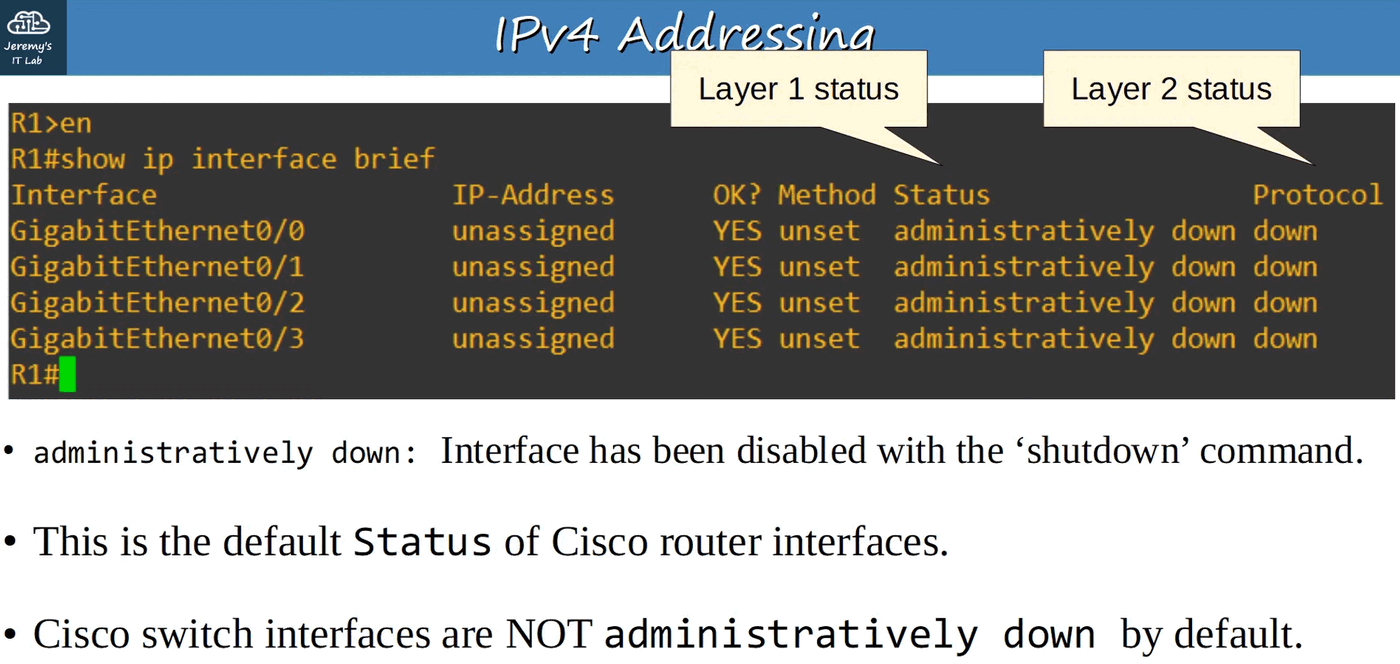
\includegraphics[keepaspectratio,alt={image}]{images/08-ipv4-addressing-part2/img-001.png}}
\end{figure}

// configure terminal cmd

R1\# conf t

// This enters interface configuration mode

R1(config)\# interface gigabitethernet 0/0

This can be shortened to `g0/0' like they are listed in physical network
maps.

\begin{figure}
\centering
\pandocbounded{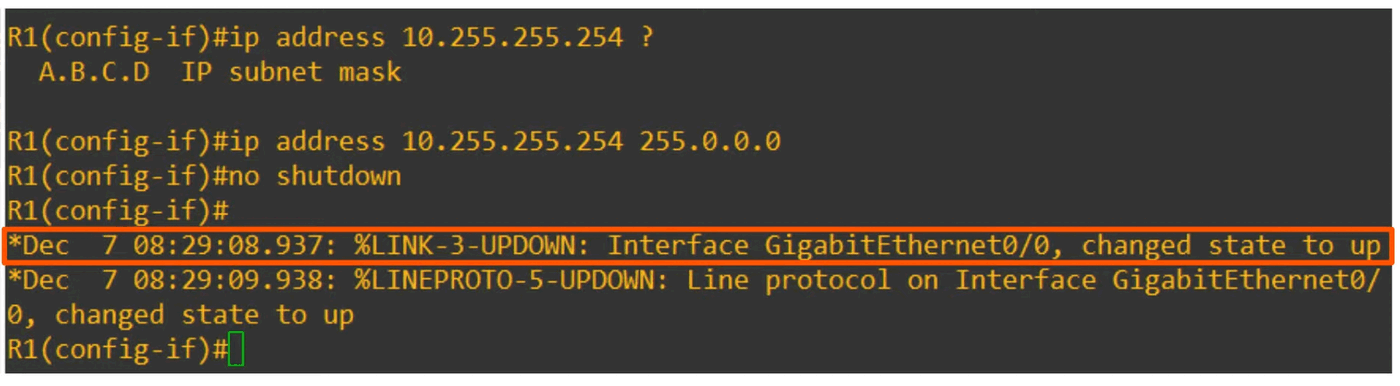
\includegraphics[keepaspectratio,alt={image}]{images/08-ipv4-addressing-part2/img-002.png}}
\end{figure}

// This sets the IP ADDRESS and SUBNET MASK of device

R1(config-if) \#ip address 10.255.255.254 255.0.0.0

// This enables the device

R1(config-if) \#no shutdown

Two messages should appear showing the state has changed to `up'
(Status). Second message should show line protocol is now `up'
(Protocol).

// `do' allows you to run a Privileged EXEC command from outside the
mode.

R1(config-if) \#do show ip interface brief

Good to confirm that the device/interface you have configured is up and
running.

More `show' CLI Commands

\begin{figure}
\centering
\pandocbounded{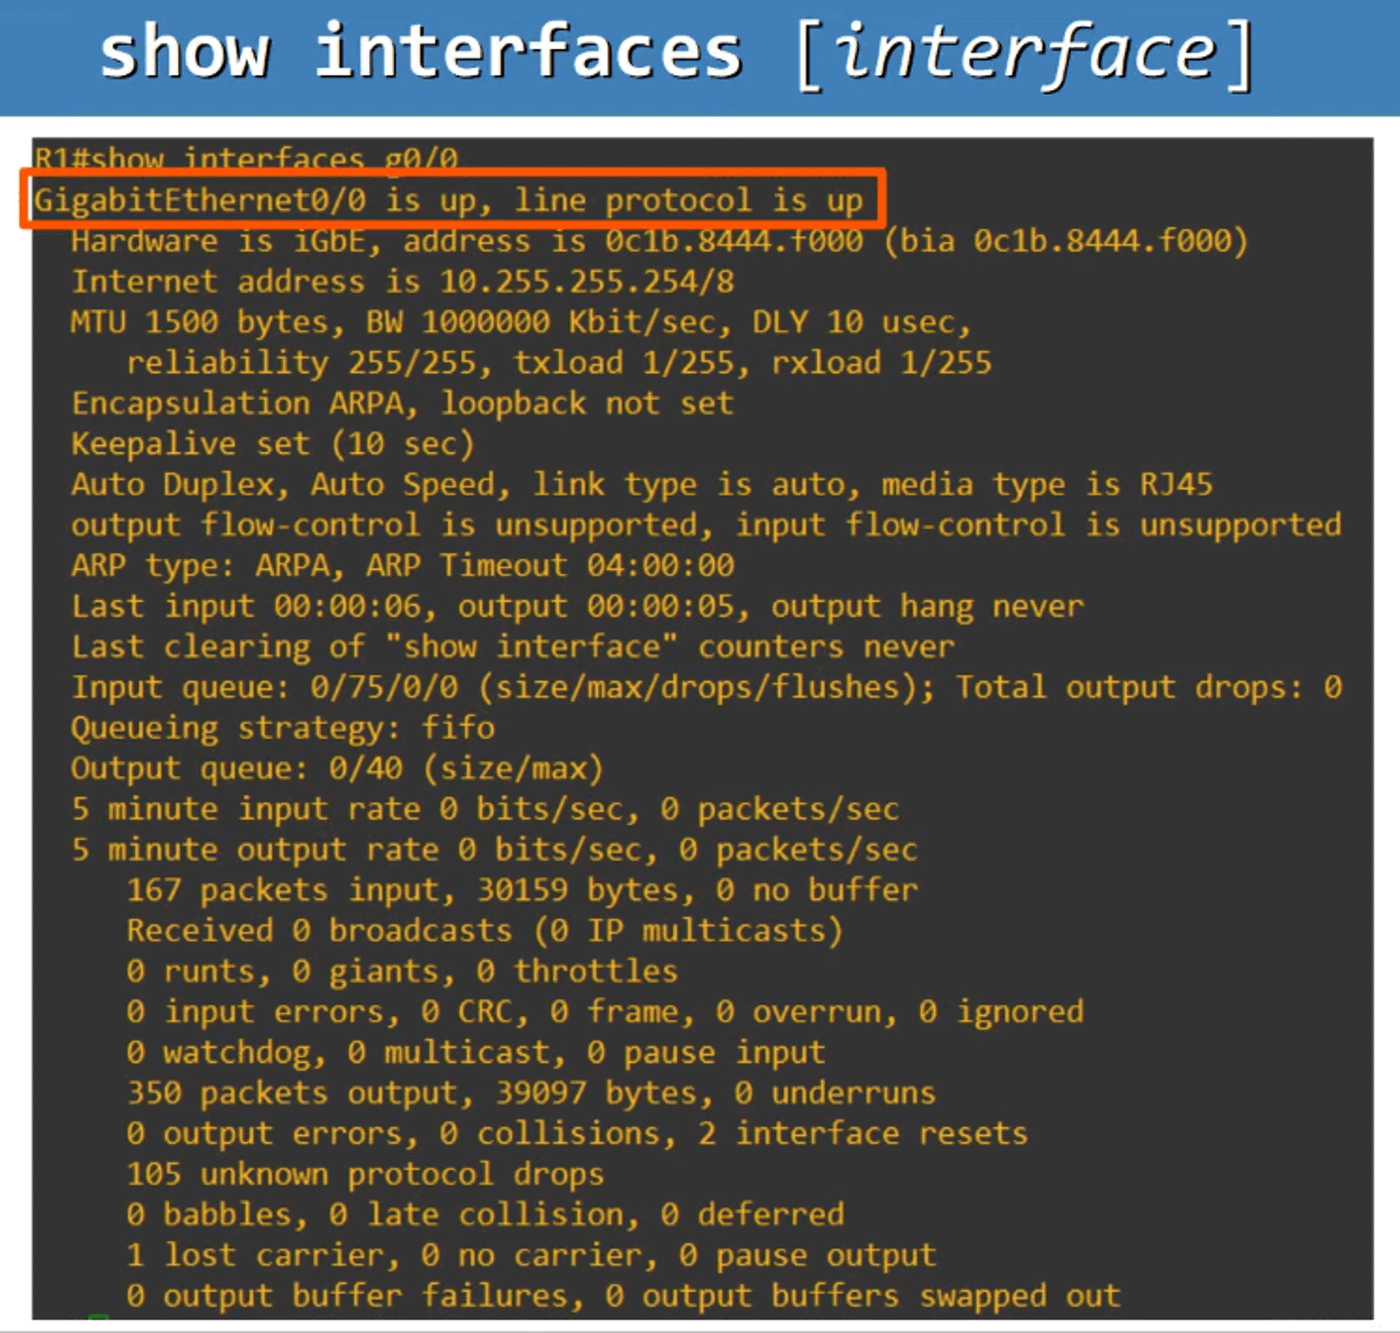
\includegraphics[keepaspectratio,alt={image}]{images/08-ipv4-addressing-part2/img-003.png}}
\end{figure}

`show interfaces \textless interface name\textgreater{}'

\begin{itemize}
\tightlist
\item
  Shows Layer 1 and Layer 2 information about the interface and some
  Layer 3.
\item
  Shows MAC Address (or BIA address)
\item
  IP Address
\item
  \ldots{} and so much more
\end{itemize}

`show interfaces description'

\begin{itemize}
\tightlist
\item
  show description for interface.
\end{itemize}

Example:

// Configure mode for interface Gigabyte Interface 0/0

R1(config) \#int g0/0

R1(config) \#description \#\# to SW1 \#\#

This sets the `Description' column to display:

\begin{lstlisting}
Interface               Description
\end{lstlisting}

Gi0/0 \#\# to SW1 \#\#

\chapter{Switch Interfaces}\label{switch-interfaces}

\begin{figure}
\centering
\pandocbounded{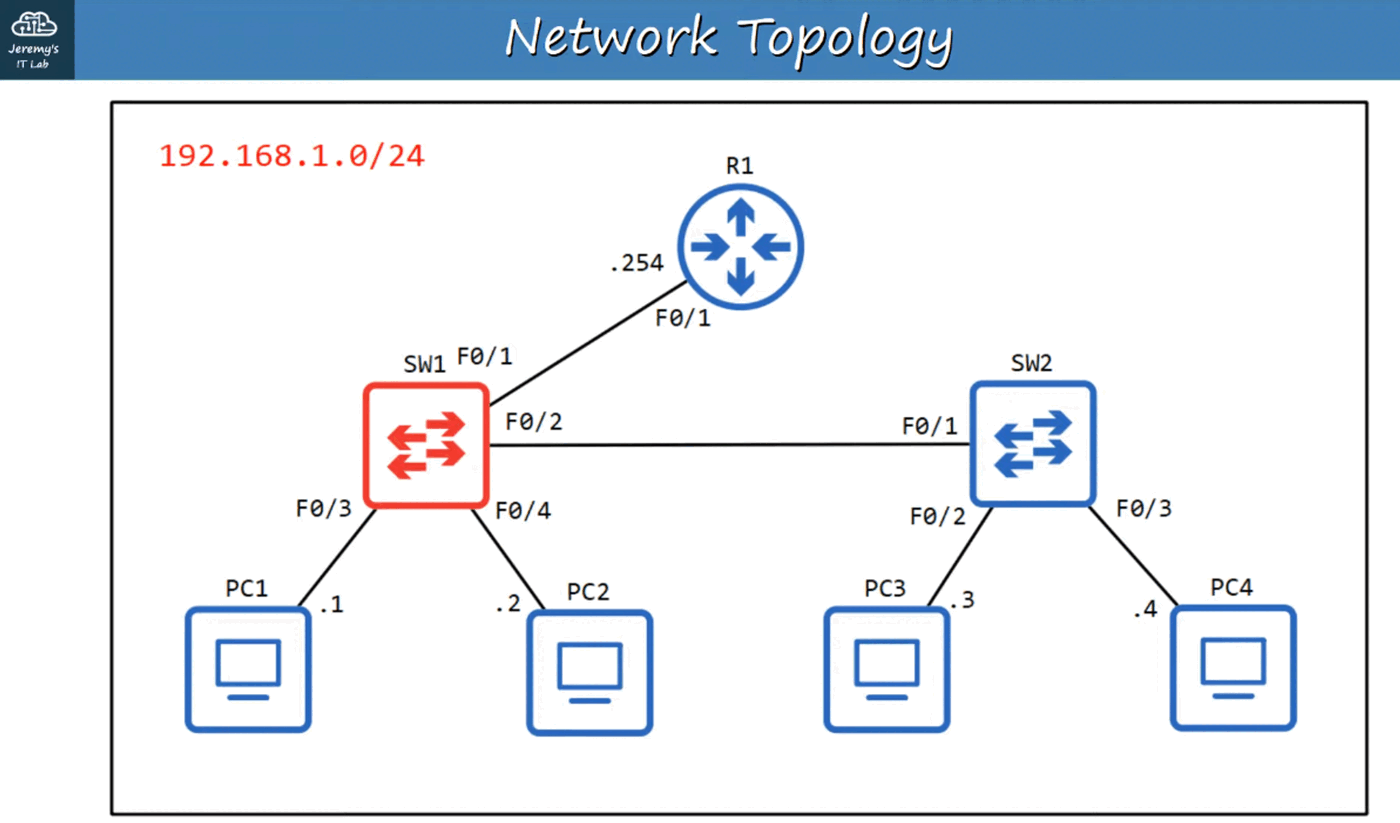
\includegraphics[keepaspectratio,alt={image}]{images/09-switch-interfaces/img-001.png}}
\end{figure}

CISCO CLI for SWITCHES

\begin{figure}
\centering
\pandocbounded{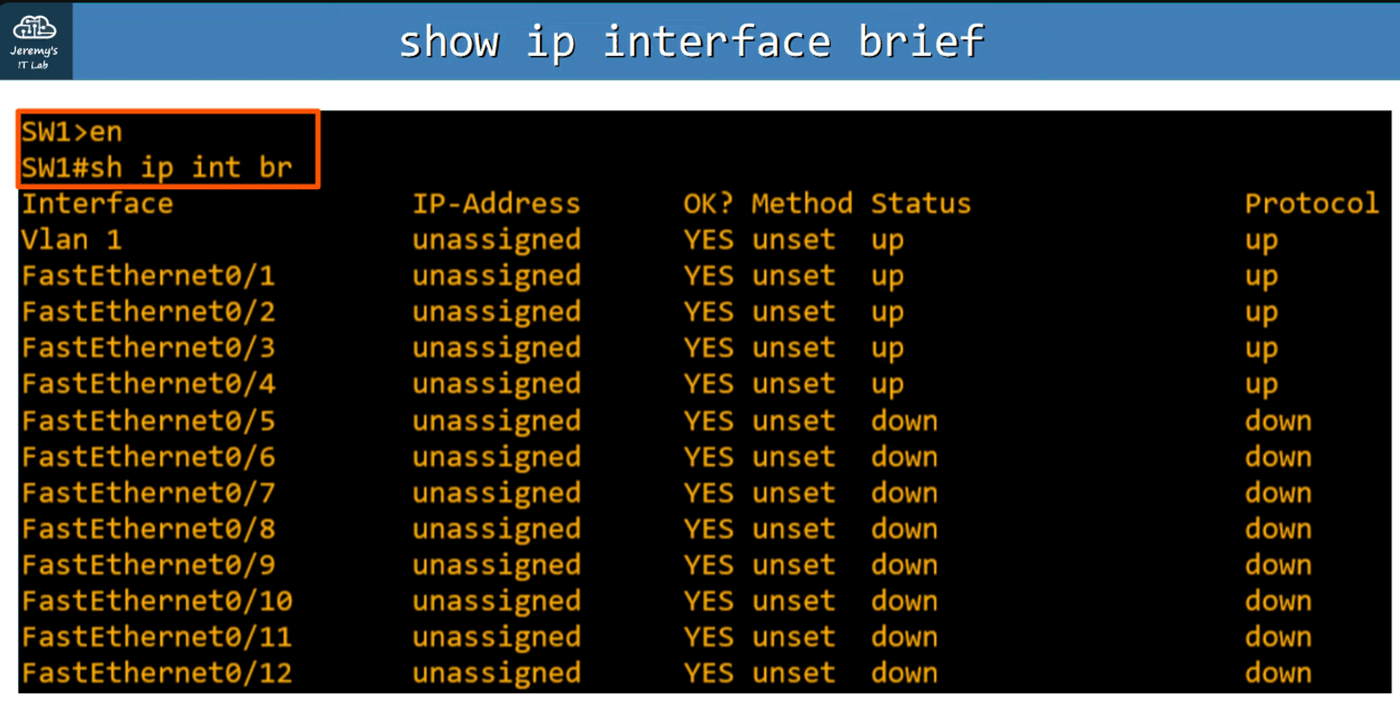
\includegraphics[keepaspectratio,alt={image}]{images/09-switch-interfaces/img-002.png}}
\end{figure}

// enter Privileged EXEC mode

SW1\textgreater enable

// Show all interfaces of Switch 1.

SW\# show ip interface brief

This will show the interfaces currently on Switch 1. It has the same
information structure as Cisco Routers.

Notice the Status (Layer 2) and Protocol (Layer 1) columns are showing
``up/up''.

Unlike ROUTERS, SWITCHES do no DEFAULT to `administrative
down/down'(shutdown).

Unconnected devices will show as ``down'' and ``down'' (not connected to
another device)

\begin{figure}
\centering
\pandocbounded{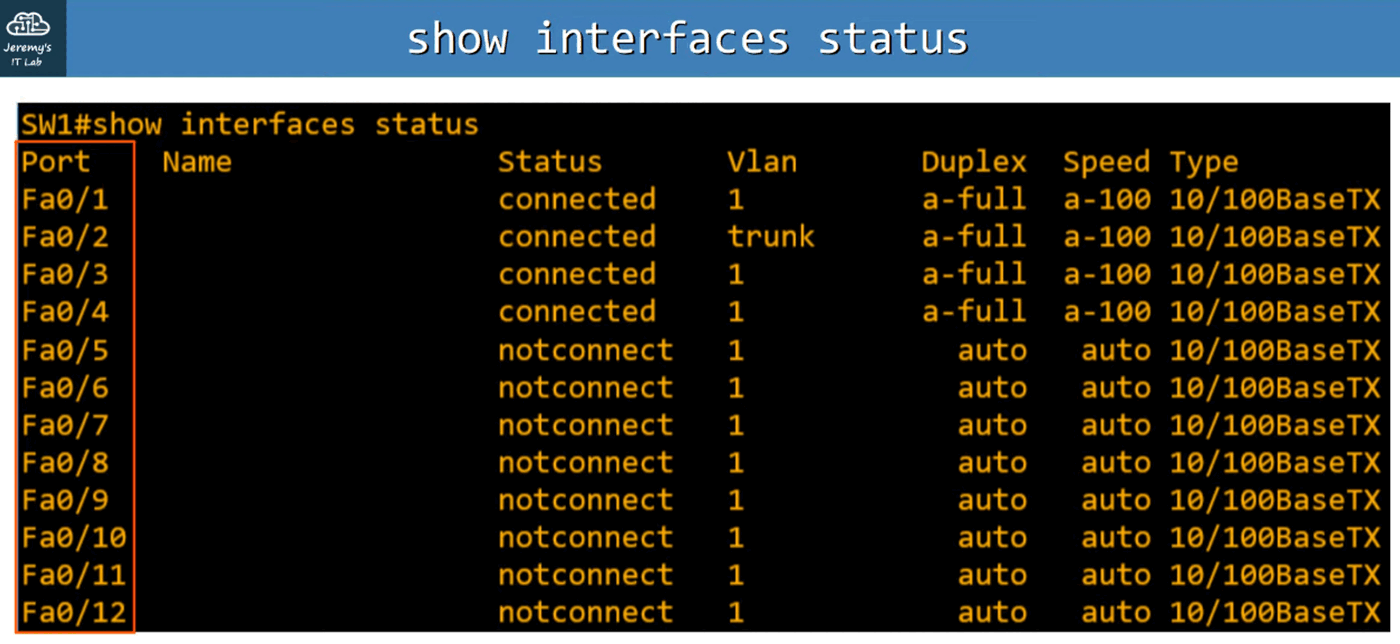
\includegraphics[keepaspectratio,alt={image}]{images/09-switch-interfaces/img-003.png}}
\end{figure}

// Show the status of all interfaces on SW1

SW1\#show interfaces status

This will list:

\begin{itemize}
\tightlist
\item
  Ports
\item
  Name (which is description)
\item
  Status (connection status)
\item
  Vlan (can be used to divide up LANs) - Vlan 1 is the default.
\item
  Duplex (can the connection send/receive at same time?) - Auto is
  default
\item
  Speed (speed in bps) - Auto is default
\item
  Type (what medium is being used, speed of interface)
\end{itemize}

\begin{figure}
\centering
\pandocbounded{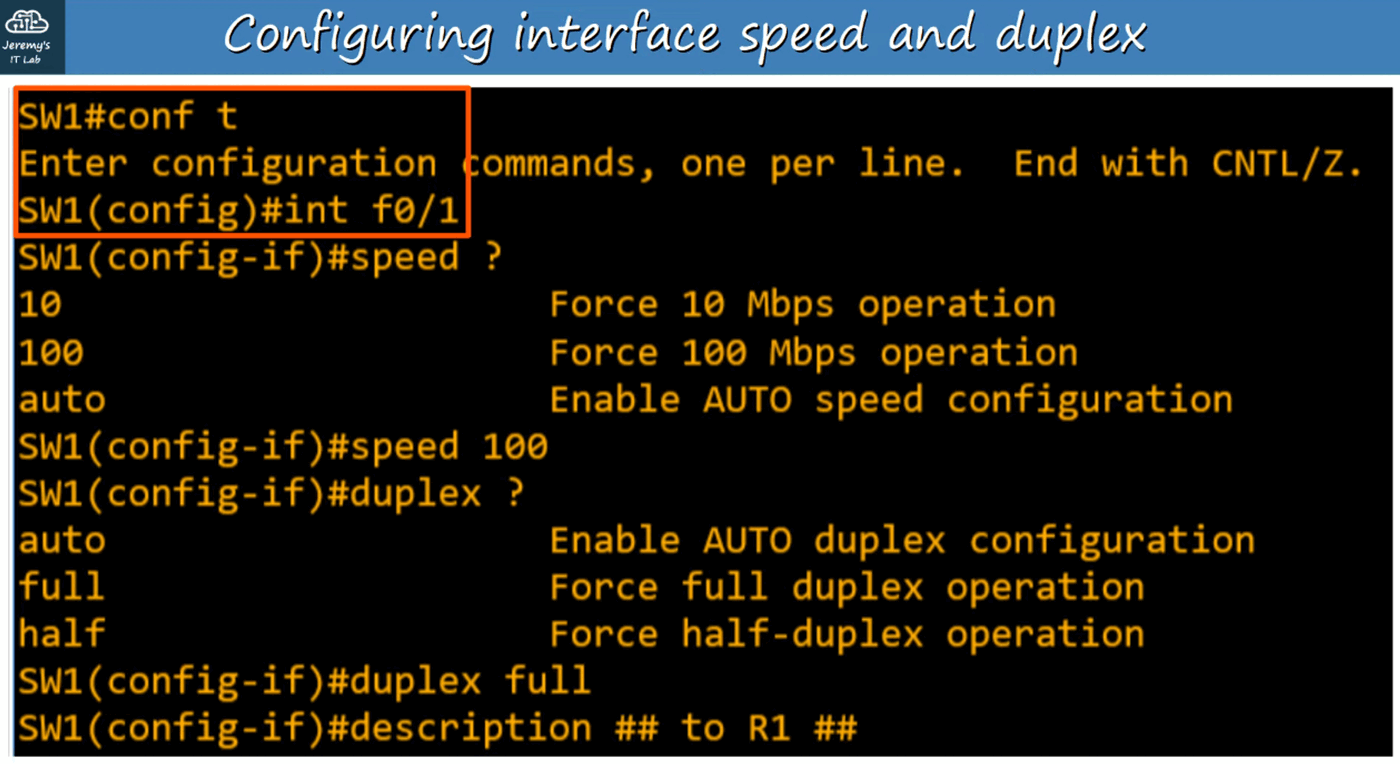
\includegraphics[keepaspectratio,alt={image}]{images/09-switch-interfaces/img-004.png}}
\end{figure}

\begin{figure}
\centering
\pandocbounded{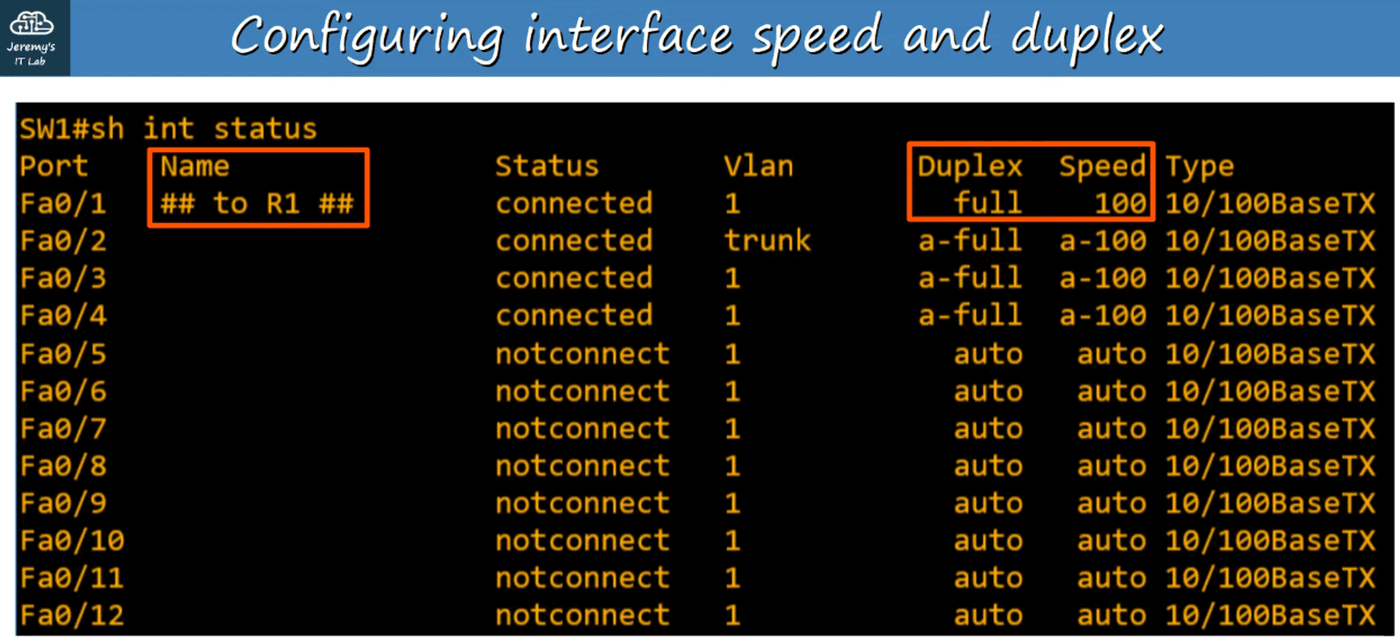
\includegraphics[keepaspectratio,alt={image}]{images/09-switch-interfaces/img-005.png}}
\end{figure}

\section{Interface Range}\label{interface-range}

Unused Interfaces can pose a security risk so it's a good idea to
deactivate them.

However, if you have 28+ interfaces not in use, do you have to do them
one at a time?

Answer: No! There is a command to apply configurations to a range of
interfaces.

Inside Global Config Mode (config t):

\begin{figure}
\centering
\pandocbounded{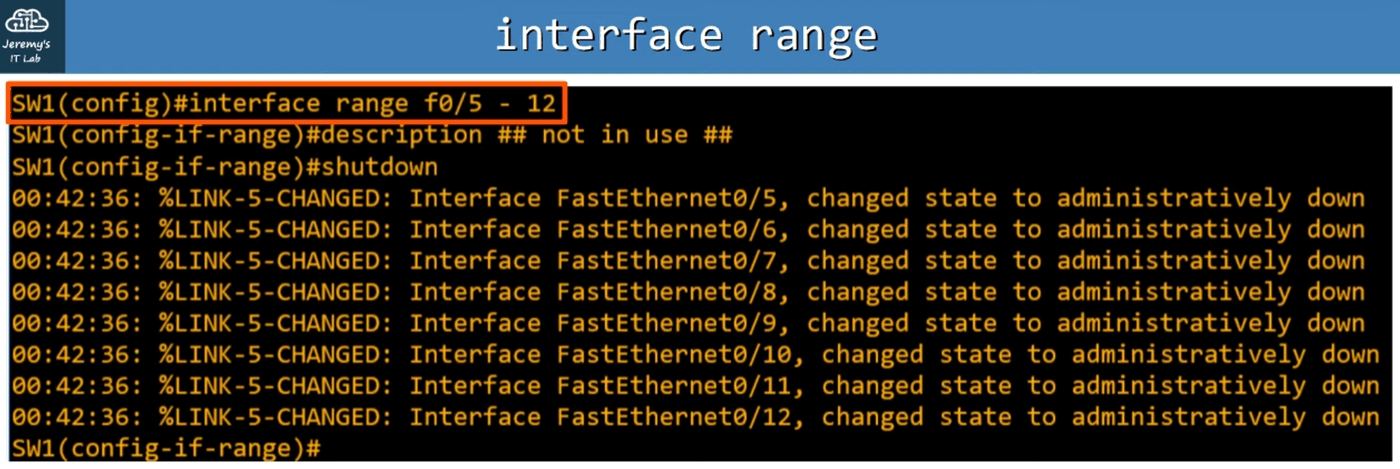
\includegraphics[keepaspectratio,alt={image}]{images/09-switch-interfaces/img-006.png}}
\end{figure}

SW1(config)\#interface range f0/5 - 12 // Choose all interfaces from 0/5
to 0/12

SW1(config-if-range)\#description \#\# not in use \#\#

SW1(config-if-range)\#shutdown

\textless\textless{} this will list all the interfaces being set to
administratively down \textgreater\textgreater{}

Confirm with `show interface status' in Privileged EXEC mode or if in
CONFIG mode, use `do show interface status'

\begin{figure}
\centering
\pandocbounded{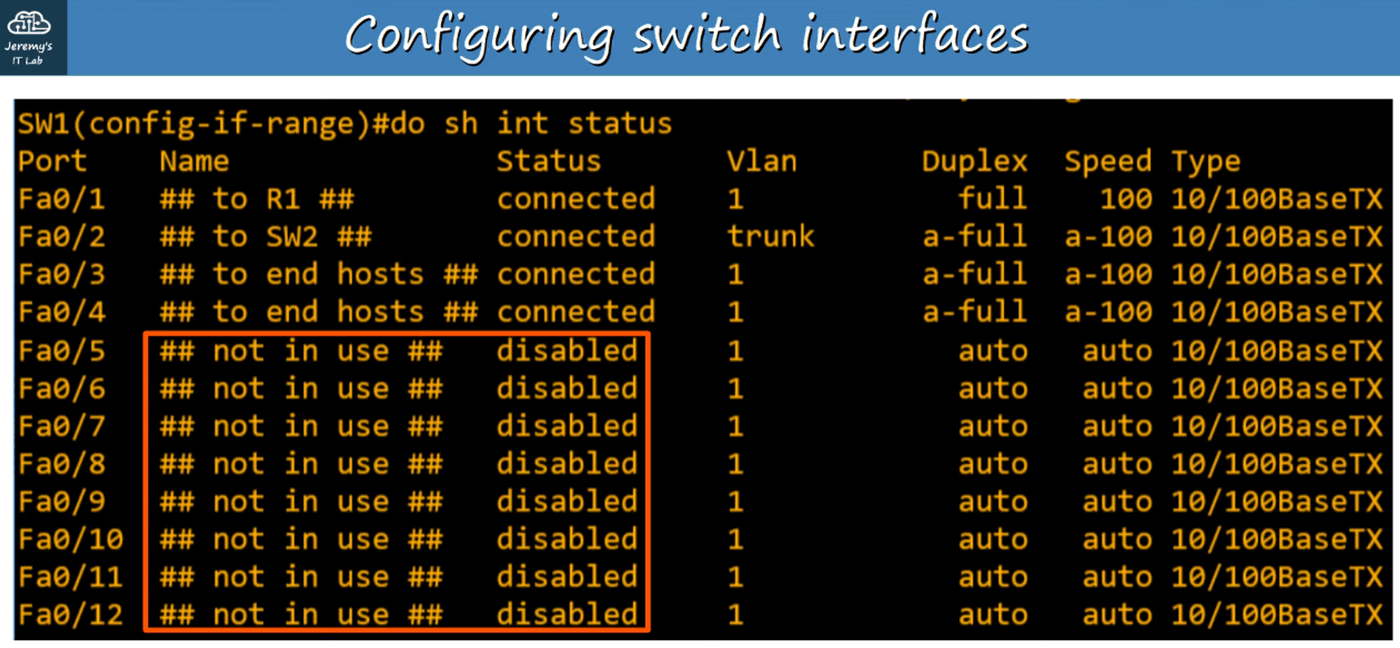
\includegraphics[keepaspectratio,alt={image}]{images/09-switch-interfaces/img-007.png}}
\end{figure}

\section{Full / Half Duplex}\label{full-half-duplex}

\section{Half Duplex}\label{half-duplex}

\begin{itemize}
\tightlist
\item
  Device cannot send / receive data at the same time. If it is receiving
  a frame, it must wait before sending a frame.
\end{itemize}

\section{Full Duplex}\label{full-duplex}

\begin{itemize}
\tightlist
\item
  Device CAN send / receive data at the same time. It does NOT have to
  wait.
\end{itemize}

MOST modern SWITCHES support FULL DUPLEX.

WHERE is HALF DUPLEX used? Almost nowhere.

In the past, LAN HUBS used HALF DUPLEX.

When multiple packets were received by the HUB, the HUB would simple
FLOOD the connections with frame data, causing a COLLISION (on the
interface), and hosts would not receive the frame intact.

All devices connected to a HUB are called a COLLISION DOMAIN.

To DEAL with COLLISIONS, Ethernet devices use a mechanism called
CSMA/CD.

CSMA/CD = CARRIER SENSE MULTIPLE ACCESS with COLLISION DETECTION.

\begin{itemize}
\tightlist
\item
  Before sending frames, devices `listen' to the collision domain until
  they detect that other devices are not sending.
\item
  IF a collision occurs, the device sends a jamming signal to inform the
  other devices that a collision happened.
\item
  Each device will wait a random period of time before sending frames
  again.
\item
  The process repeats.
\end{itemize}

SWITCHES are more sophisticated than HUBS.

HUBS are Layer 1 Devices - Collisions are common and use CSMA/CD.
SWITCHES are Layer 2 Devices - Collisions RARELY occur.

\begin{figure}
\centering
\pandocbounded{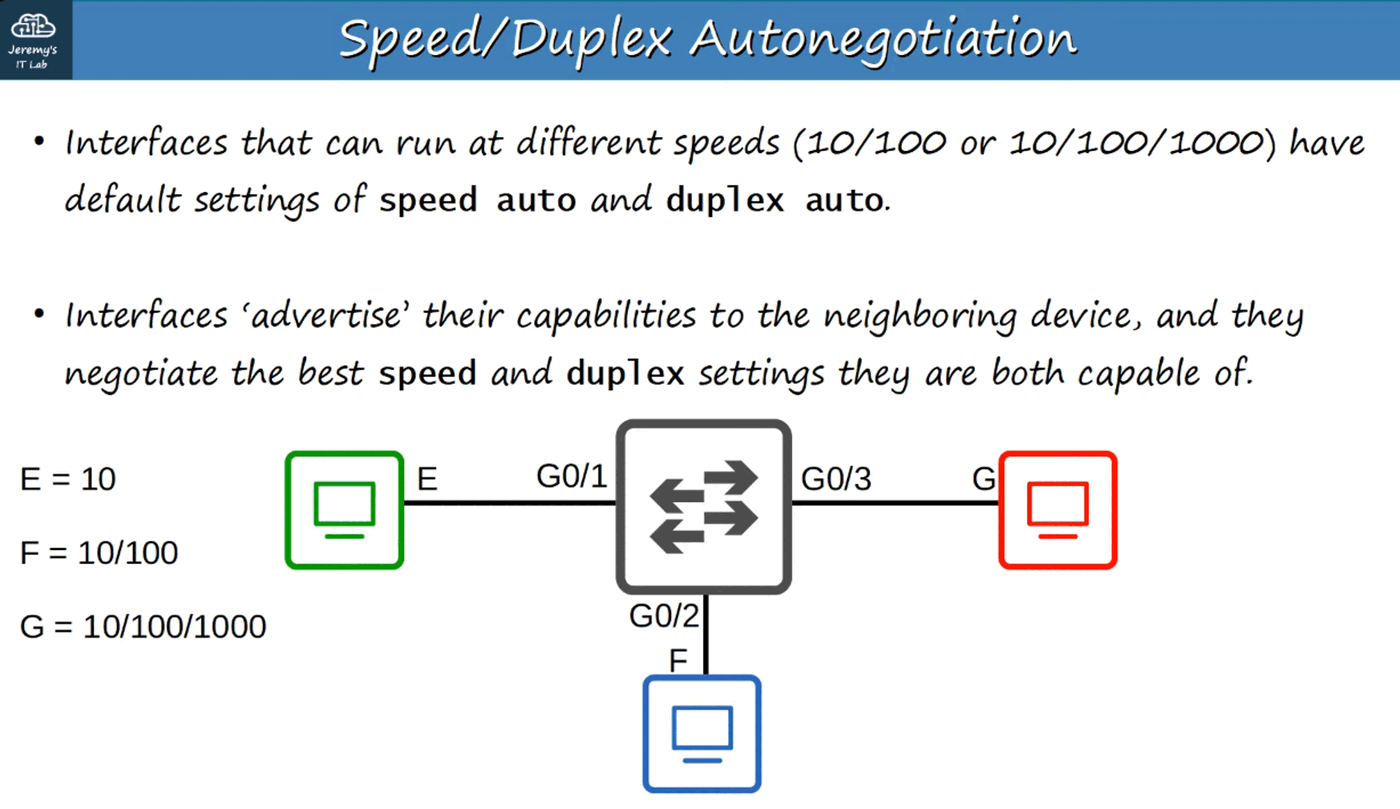
\includegraphics[keepaspectratio,alt={image}]{images/09-switch-interfaces/img-008.png}}
\end{figure}

\section{Speed / Duplex
Autonegotiation}\label{speed-duplex-autonegotiation}

\begin{itemize}
\tightlist
\item
  Interfaces that can run at different speeds (10/100 or 10/100/1000)
  have a default setting of SPEED AUTO and DUPLEX AUTO.
\item
  Interfaces `advertise' their capabilities to the neighbouring device,
  and they negotiate the best SPEED and DUPLEX settings they are both
  capable of.
\end{itemize}

WHAT if AUTONEGOTIATION is DISABLED on the device connected to the
SWITCH ?

\begin{figure}
\centering
\pandocbounded{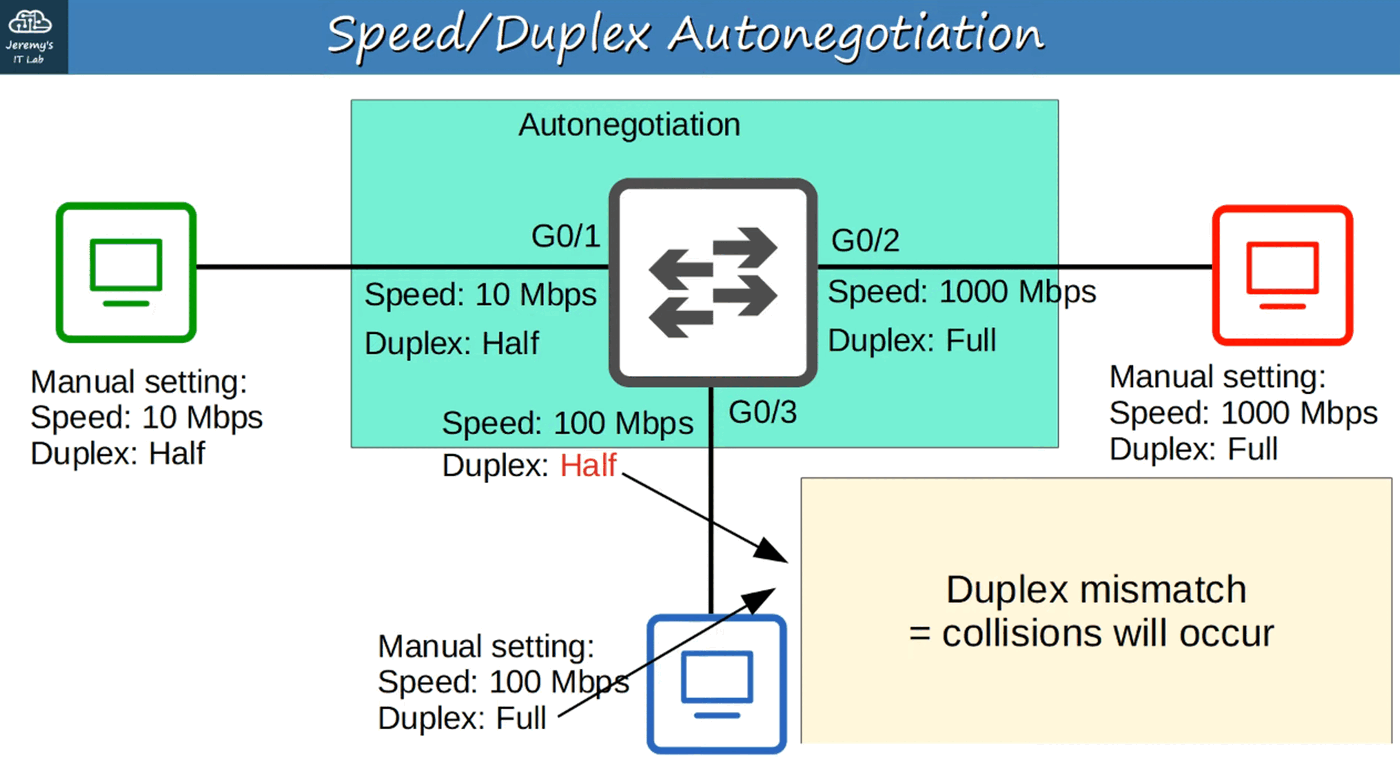
\includegraphics[keepaspectratio,alt={image}]{images/09-switch-interfaces/img-009.png}}
\end{figure}

\begin{itemize}
\tightlist
\item
  SPEED: The SWITCH will try to send at the speed that the other device
  is operating at. If it fails to send the speed, it will use the
  slowest supported speed (ie: 10 Mbps on a 10/100/1000 interface).
\item
  DUPLEX: If the speed is 10 or 100 Mbps the SWITCH will use HALF
  DUPLEX. If the speed is 1000 Mbps or great, it will use FULL DUPLEX.
\end{itemize}

\section{Interface Counters and
Errors}\label{interface-counters-and-errors}

Show using the:

// Privileged EXEC mode

SW1\#show interfaces \textless interface name\textgreater{}

Error stats will be at the bottom.

\begin{figure}
\centering
\pandocbounded{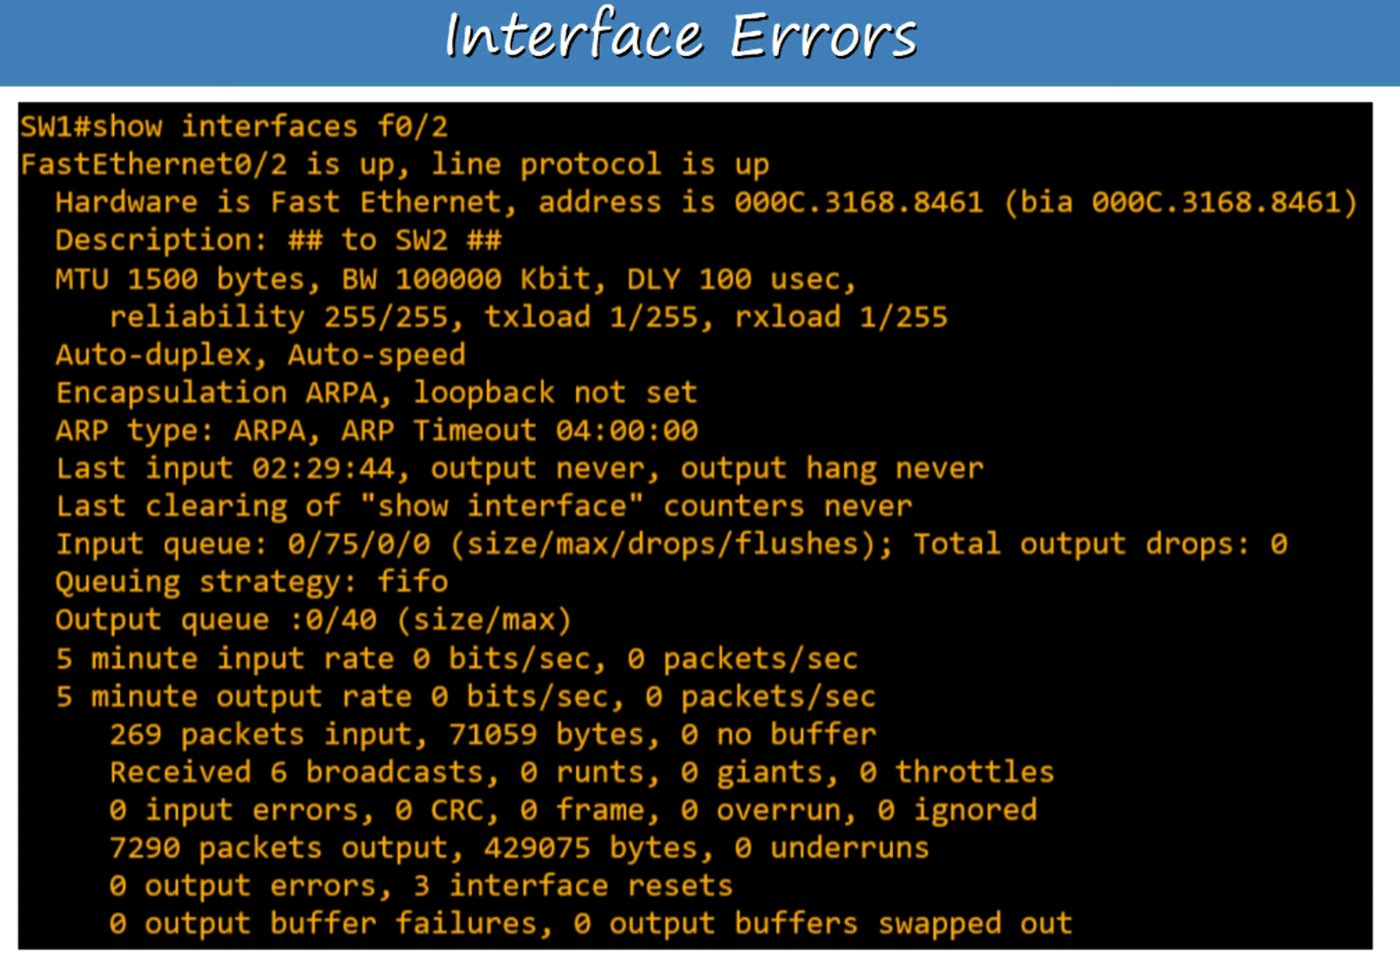
\includegraphics[keepaspectratio,alt={image}]{images/09-switch-interfaces/img-010.png}}
\end{figure}

\textbf{Packets Received / Total bytes received.}

\textbf{Runts}: Frames that are smaller than the minimum frame size (64
bytes)

\textbf{Giants}: Frames that are larger than the maximum frame size
(1518 bytes)

\textbf{CRC}: Frames that failed the CRC check (in the Ethernet FCS
trailer)

\textbf{Frame}: Frames that have an incorrect format (due to an error)

\textbf{Input errors}: Total of various counters, such as the above four

\textbf{Output errors}: Frames the SWITCH tried to send, but failed due
to an error

\chapter{The IPv4 Header}\label{the-ipv4-header}

INTERNET PROTOCOL version 4 HEADER or IPv4 HEADER

HEADER is used at LAYER 3 to help send data between devices on separate
networks, even on other sides of the world over the Internet.

This is known as ROUTING.

THE IPv4 HEADER is used to ENCAPSULATE a TCP or UDP Segment.

To Review:

\begin{figure}
\centering
\pandocbounded{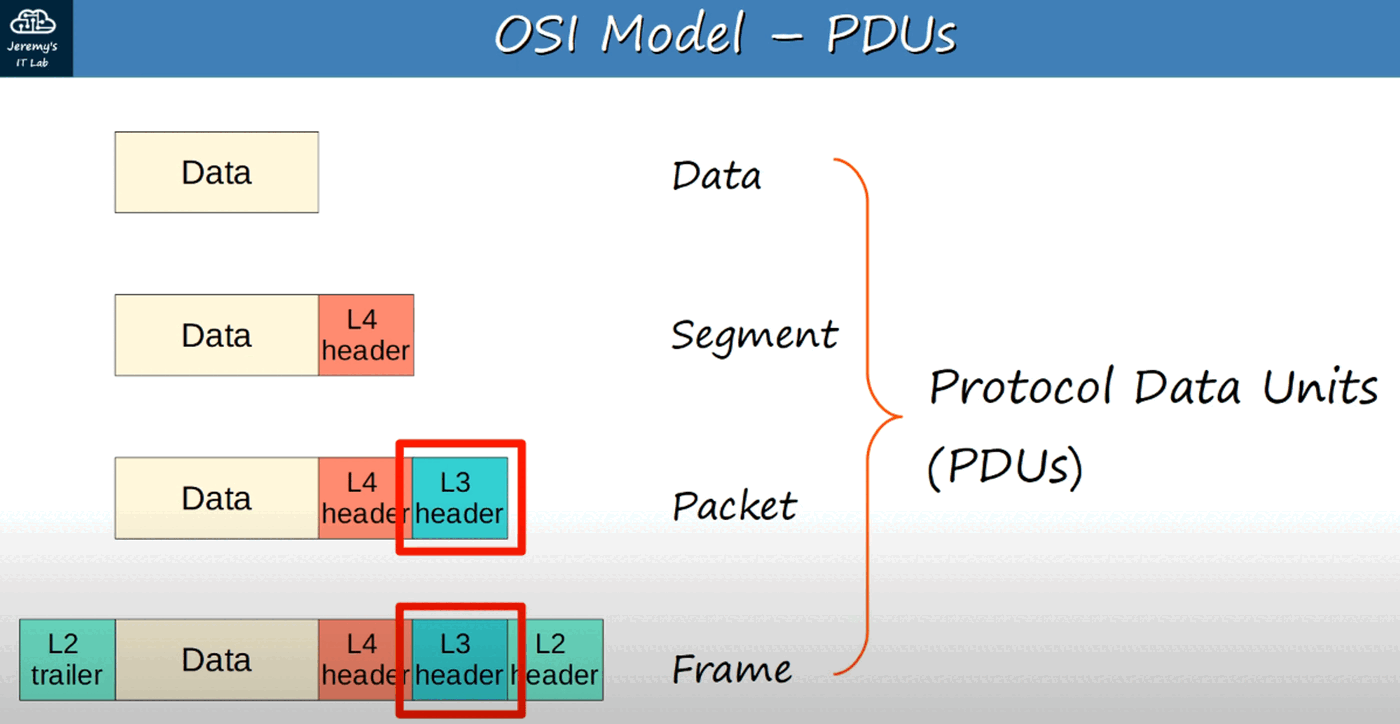
\includegraphics[keepaspectratio,alt={image}]{images/10-the-ipv4-header/img-001.png}}
\end{figure}

FIELDS OF THE IPv4 HEADER

\begin{figure}
\centering
\pandocbounded{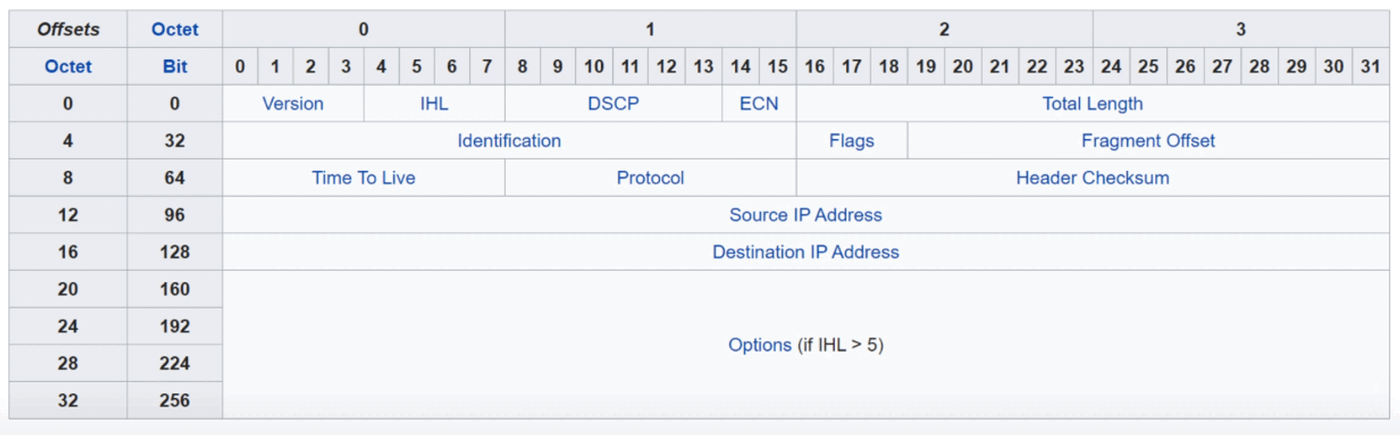
\includegraphics[keepaspectratio,alt={image}]{images/10-the-ipv4-header/img-002.png}}
\end{figure}

{\def\LTcaptype{none} % do not increment counter
\begin{longtable}[]{@{}ll@{}}
\toprule\noalign{}
FIELD & \# OF BITS \\
\midrule\noalign{}
\endhead
\bottomrule\noalign{}
\endlastfoot
VERSION & 4 \\
IHL & 4 \\
DSCP & 6 \\
ECN & 2 \\
TOTAL LENGTH & 16 \\
IDENTIFICATION & 16 \\
FLAGS & 3 \\
FRAGMENT OFFSET & 13 \\
TIME TO LIVE & 8 \\
PROTOCOL & 8 \\
HEADER CHECKSUM & 16 \\
SOURCE ADDRESS & 32 \\
DESTINATION ADDRESS & 32 \\
OPTIONS & 320 Max \\
\end{longtable}
}

\section{Version}\label{version}

\begin{itemize}
\tightlist
\item
  LENGTH is 4 bits.
\item
  IDs version of IP used (IPv4 or IPv6)

  \begin{itemize}
  \tightlist
  \item
    IPv4 = 0100 in Binary (Decimal 4)
  \item
    IPv6 = 0110 in Binary (Decimal 6)
  \end{itemize}
\end{itemize}

\section{Internet Header Length (IHL)}\label{internet-header-length-ihl}

\begin{itemize}
\tightlist
\item
  LENGTH is 4 bits.
\item
  Final field of IPv4 Header (Options) is variable in length so this
  field is necessary to indicate the total length of the header.
\item
  IDs the length of the header in 4-BYTE INCREMENTS.
\item
  The MINIMUM value is 5 (5 * 4-bytes = 20 bytes) - Empty OPTIONS Field
\item
  The MAXIMUM value is 15 (15 * 4-bytes = 60 bytes)
\end{itemize}

MINIMUM IPv4 HEADER LENGTH = 20 Bytes! MAXIMUM IPv4 HEADER LENGTH = 60
Bytes!

DSCP (Differentiated Services Code Point):

\begin{itemize}
\tightlist
\item
  LENGTH is 6 bits.
\item
  Used for QoS (Quality of Service)
\item
  Used to prioritize delay-sensitive data (streaming voice, video, etc.)
\end{itemize}

ECN (Explicit Congestion Notification):

\begin{itemize}
\tightlist
\item
  LENGTH is 2 bits.
\item
  Provides end-to-end (between two endpoints) notification of network
  congestion WITHOUT dropping packets.
\item
  Optional feature that requires both endpoints, as well as the
  underlying network infrastructure to support it.
\end{itemize}

\section{Total Length}\label{total-length}

\begin{itemize}
\tightlist
\item
  LENGTH is 16 bits.
\item
  Indicates the TOTAL length of the packet (L3 Header + L4 Segment)
\item
  Measured in bytes (not 4-byte increments like IHL)
\item
  Minimum value of 20 Bytes (IPv4 Header with NO encapsulated data)
\item
  Maximum value of 65,535 (MAXIMUM 16-bit value) = 2\^{}16
\end{itemize}

\section{Identification}\label{identification}

\begin{itemize}
\tightlist
\item
  LENGTH is 16 bits.
\item
  If a packet is fragmented due to being too large, this field is used
  to identify which packet the fragment belongs to.
\item
  All fragments of the same packet will have their own IPv4 header with
  the same value in this field.
\item
  Packets are fragmented, if larger than the MTU (Maximum Transmission
  Unit)
\item
  The MTU is usually 1500 bytes (Max size of an Ethernet frame)
\item
  Fragments are reassembled by the receiving host.
\end{itemize}

\section{Flags}\label{flags}

\begin{itemize}
\tightlist
\item
  LENGTH is 3 bits
\item
  Used to control/identify fragments.
\item
  Bit 0: Reserved, always set to 0.
\item
  Bit 1: Don't Fragment (DF bit), used to indicate a packet that should
  not be fragmented.
\item
  Bit 2: More Fragments (MF bit), set to 1 if there are more fragments
  in the packet, set to 0 for the last fragment or NO fragments.
\end{itemize}

\section{Fragment Offset}\label{fragment-offset}

\begin{itemize}
\tightlist
\item
  LENGTH is 13 bits
\item
  Used to indicated the position of the fragment within the original,
  unfragmented IP Packet.
\item
  Allows fragmented packets to be reassembled even if the fragments
  arrive out of order.
\end{itemize}

\section{Time to Live (TTL)}\label{time-to-live-ttl}

\begin{itemize}
\tightlist
\item
  LENGTH is 8 bits
\item
  A router will drop a packet with a TTL of 0
\item
  Used to prevent infinite loops
\item
  Originally designed to indicated a packets maximum lifetime in
  seconds.
\item
  In practice, indicates a `hop count': each time the packet arrives at
  a router, the router decreases the TTL by 1.
\item
  Recommended default TTL is 64.
\end{itemize}

\section{Protocol}\label{protocol}

\begin{itemize}
\tightlist
\item
  LENGTH is 8 bits
\item
  Indicates the protocol of the encapsulated Layer 4 PDU
\item
  Value of 1 : ICMP
\item
  Value of 6 : TCP
\item
  Value of 17 : UDP
\item
  Value of 89 : OSPF (Dynamic Routing Protocol)
\item
  List of protocol numbers on Wikipedia : List of IP Protocol Numbers
\end{itemize}

\section{Header Checksum}\label{header-checksum}

\begin{itemize}
\tightlist
\item
  LENGTH is 16 bits
\item
  A calculated checksum used to check for errors in the IPv4 header.
\item
  When a router receives a packet, it calculates the checksum of the
  header and compares it to the one in this field of a header.
\item
  If they do not match, the router drops the packet.
\item
  Used to check for ERRORS only in the IPv4 Header.
\item
  IP relies on the encapsulated protocol to detect errors in the
  encapsulated data.
\item
  Both TCP and UDP have their own checksum fields to detect errors in
  the encapsulated data.
\end{itemize}

SOURCE and DESTINATION:

\begin{itemize}
\tightlist
\item
  LENGTH is 32 bits each
\item
  SOURCE IP = IPv4 ADDRESS of the Sender of the Packet.
\item
  DESTINATION IP = IPv4 ADDRESS of the intended Receiver of the Packet.
\end{itemize}

\section{Options}\label{options}

\begin{itemize}
\tightlist
\item
  LENGTH is 0-320 bits
\item
  Optional / Rarely Used
\item
  If the IHL field is greater than 5, it means that Options are present.
\end{itemize}

\chapter{Routing Fundamentals: Part
1}\label{routing-fundamentals-part-1}

\subsection{WHAT IS ROUTING ?}\label{what-is-routing}

ROUTING is the process that routers use to determine the path that IP
packets should take over a network to reach their destination.

\begin{itemize}
\tightlist
\item
  ROUTERS store routes to all their known destinations in a ROUTING
  TABLE
\item
  When ROUTERS receive PACKETS, they look in the ROUTING TABLE to find
  the best route to forward that packet.
\end{itemize}

There are two main routing methods (methods that routers use to learn
routes):

\begin{itemize}
\tightlist
\item
  DYNAMIC ROUTING : ROUTERS use Dynamic Routing Protocols (ie: OSPF) to
  share routing information with each other automatically and build
  their routing tables.
\item
  STATIC ROUTING : A network engineer / Admin manually configures routes
  on the router.
\end{itemize}

A ROUTE tells the ROUTER :

\begin{itemize}
\tightlist
\item
  to send a packet to Destination X, you should send the pack to
  \textbf{\emph{next-hop}} Y
\item
  or if the Destination is directly connected to the router, \emph{send
  the packet directly to the destination.}
\item
  or if the Destination is the router's own IP address, \emph{receive
  the packet for yourself (don't forward it).}
\end{itemize}

\begin{figure}
\centering
\pandocbounded{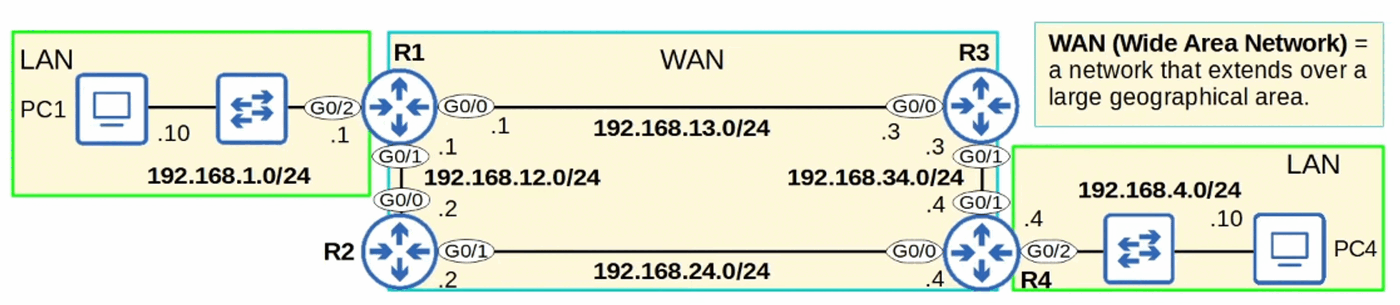
\includegraphics[keepaspectratio,alt={image}]{images/11-routing-fundamentals-part1/img-001.png}}
\end{figure}

WAN (Wide Area Network) = network that extends over a large geographic
area.

\begin{figure}
\centering
\pandocbounded{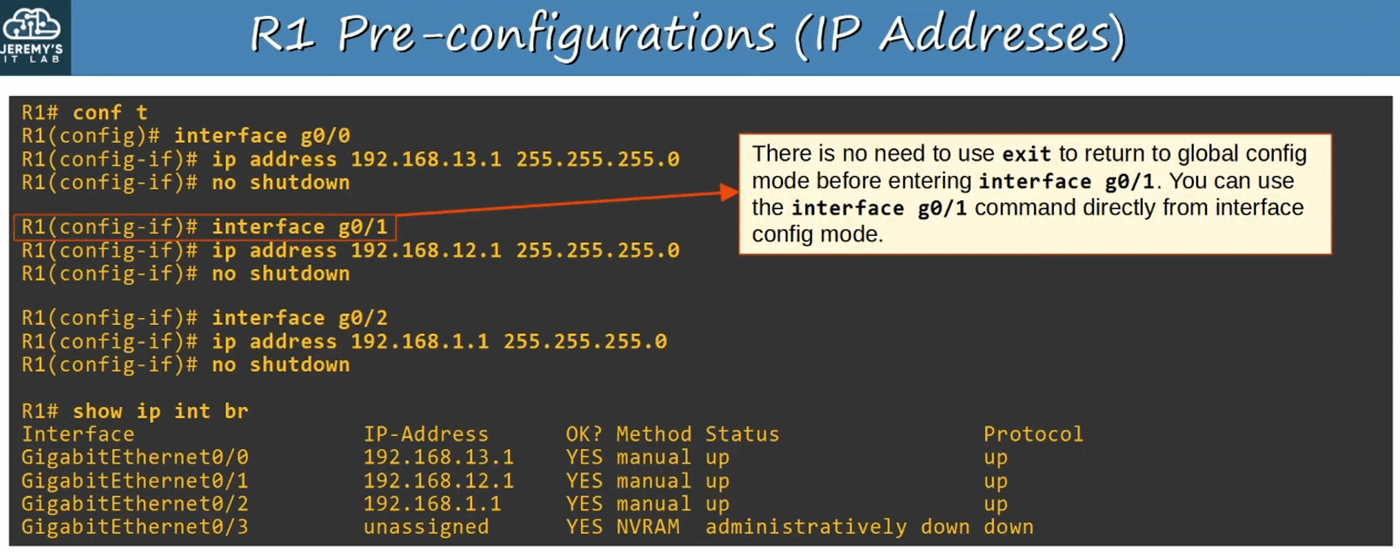
\includegraphics[keepaspectratio,alt={image}]{images/11-routing-fundamentals-part1/img-002.png}}
\end{figure}

\begin{figure}
\centering
\pandocbounded{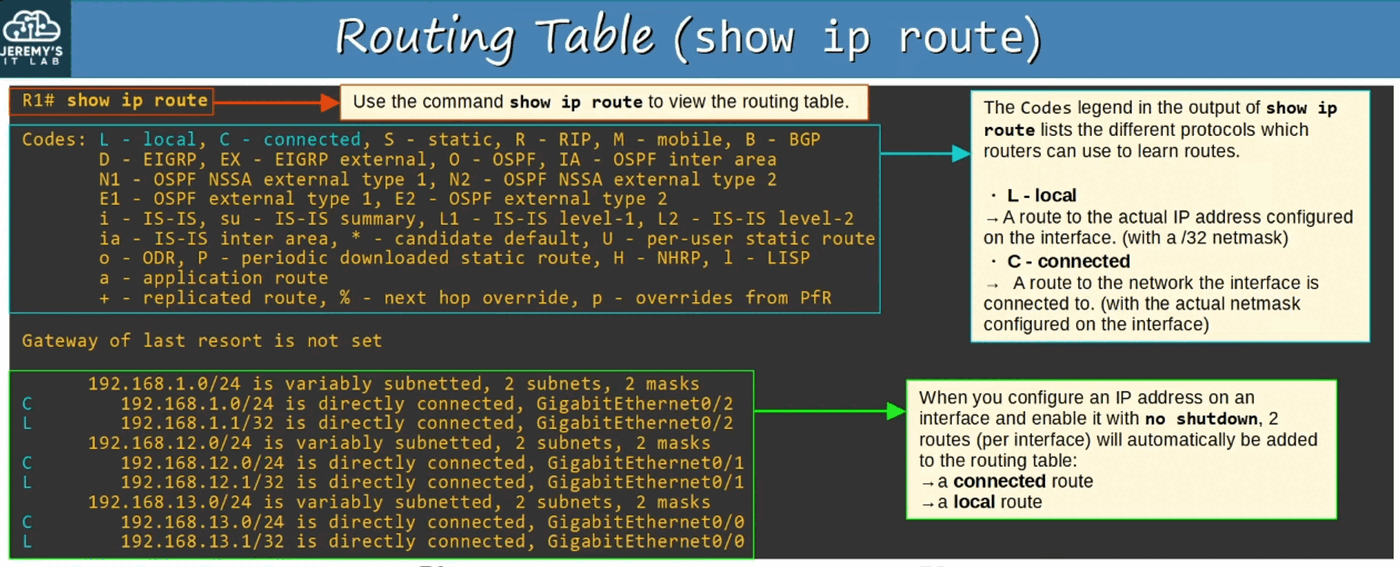
\includegraphics[keepaspectratio,alt={image}]{images/11-routing-fundamentals-part1/img-003.png}}
\end{figure}

\begin{figure}
\centering
\pandocbounded{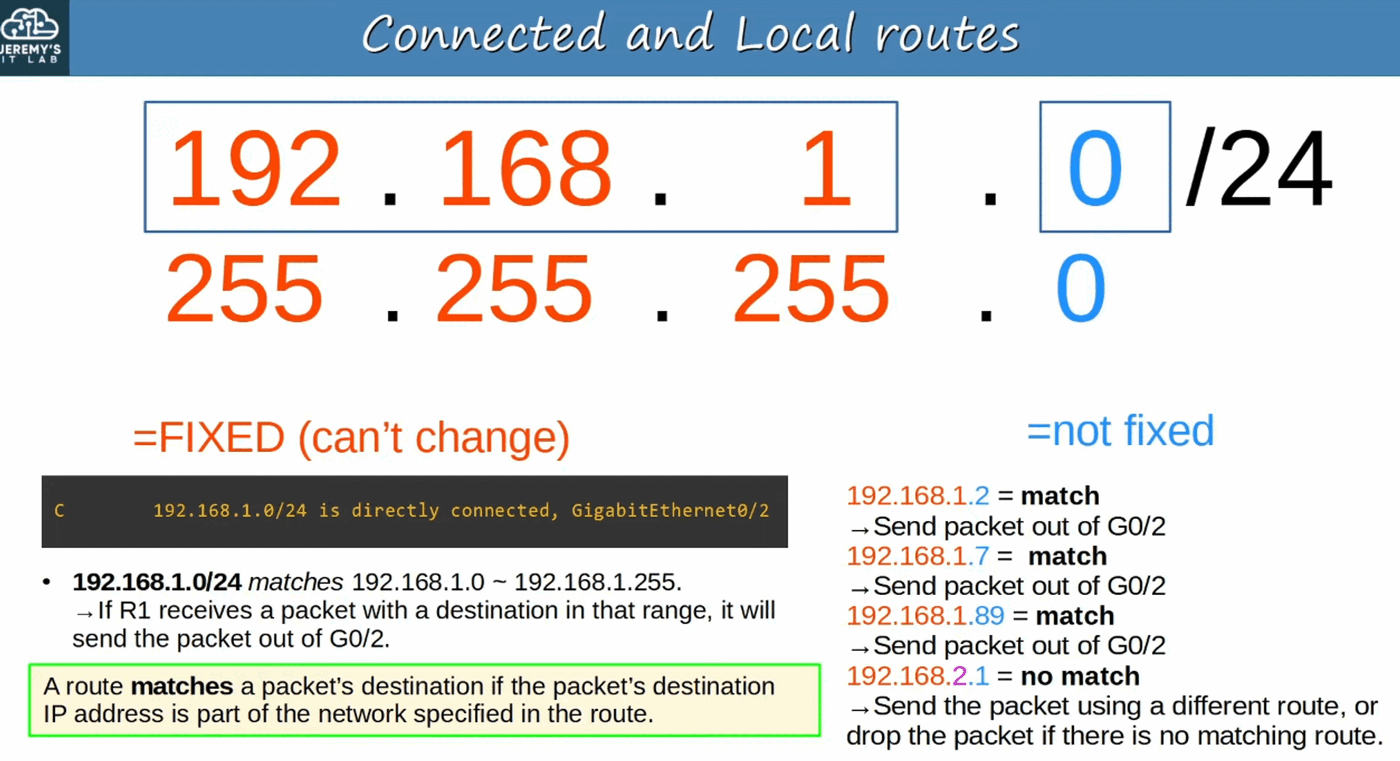
\includegraphics[keepaspectratio,alt={image}]{images/11-routing-fundamentals-part1/img-004.png}}
\end{figure}

\begin{figure}
\centering
\pandocbounded{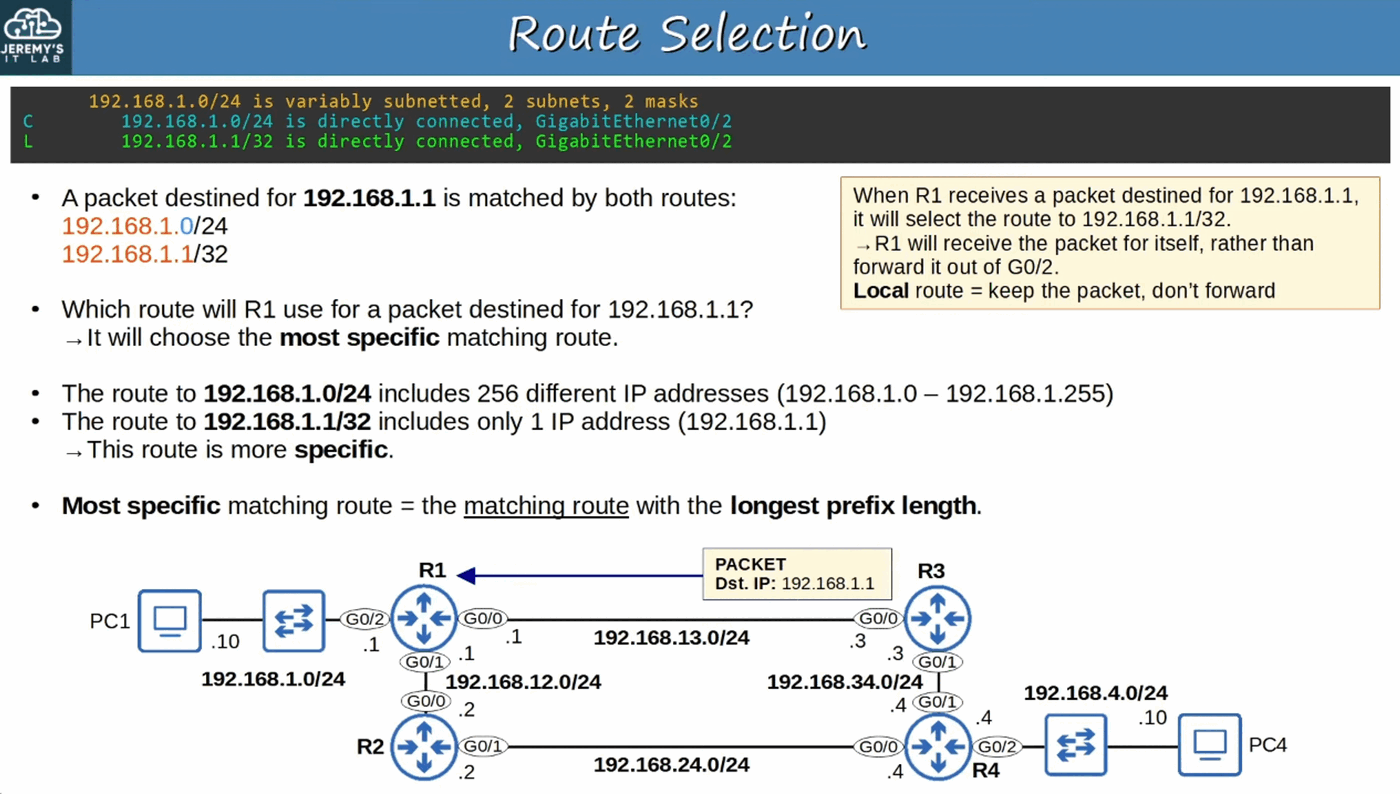
\includegraphics[keepaspectratio,alt={image}]{images/11-routing-fundamentals-part1/img-005.png}}
\end{figure}

\begin{figure}
\centering
\pandocbounded{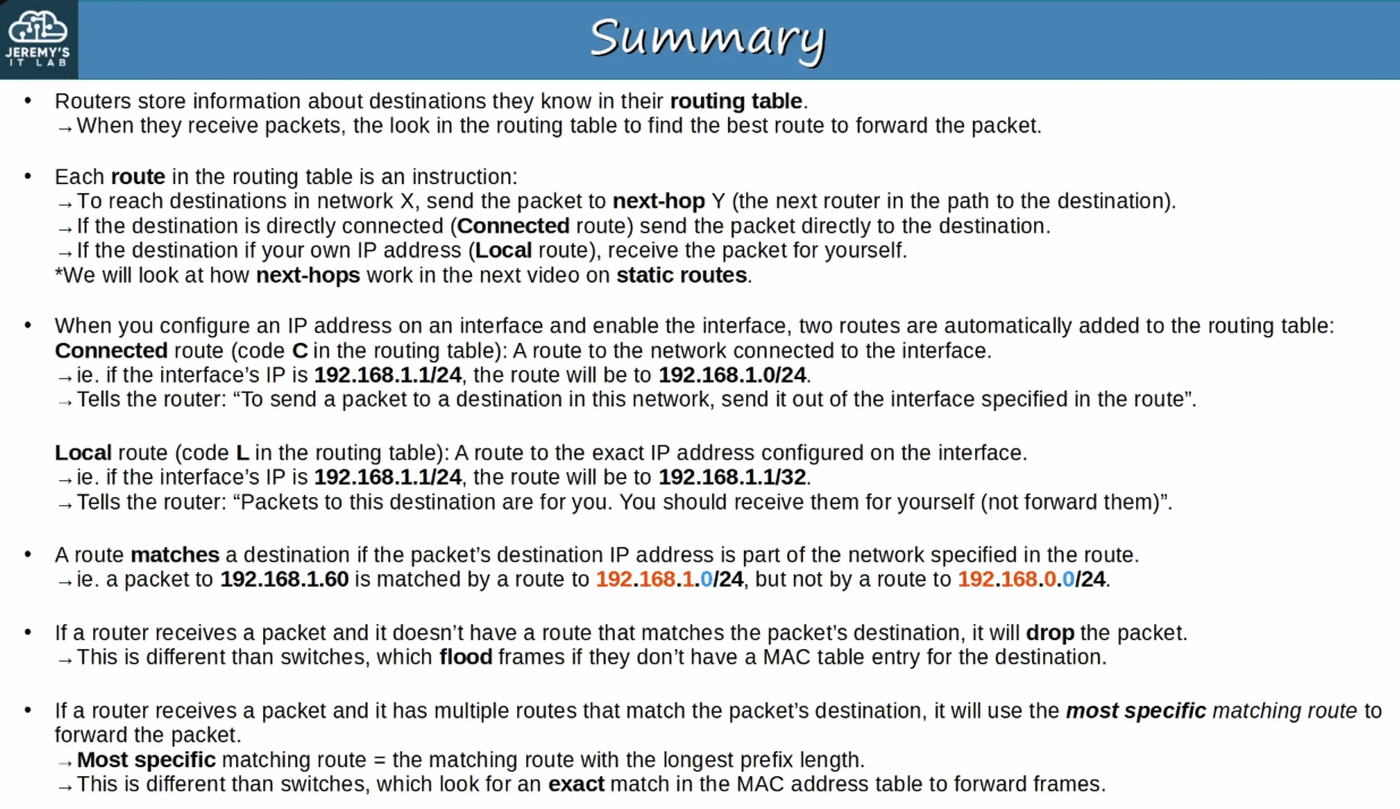
\includegraphics[keepaspectratio,alt={image}]{images/11-routing-fundamentals-part1/img-006.png}}
\end{figure}

\chapter{Static Routing: Part 2}\label{static-routing-part-2}

\section{Review}\label{review}

SWITCHES forward traffic WITHIN LAN's ROUTERS forward traffic BETWEEN
LAN's

WAN (Wide Area Network)

\begin{itemize}
\tightlist
\item
  Network spread over a large area
\end{itemize}

\begin{figure}
\centering
\pandocbounded{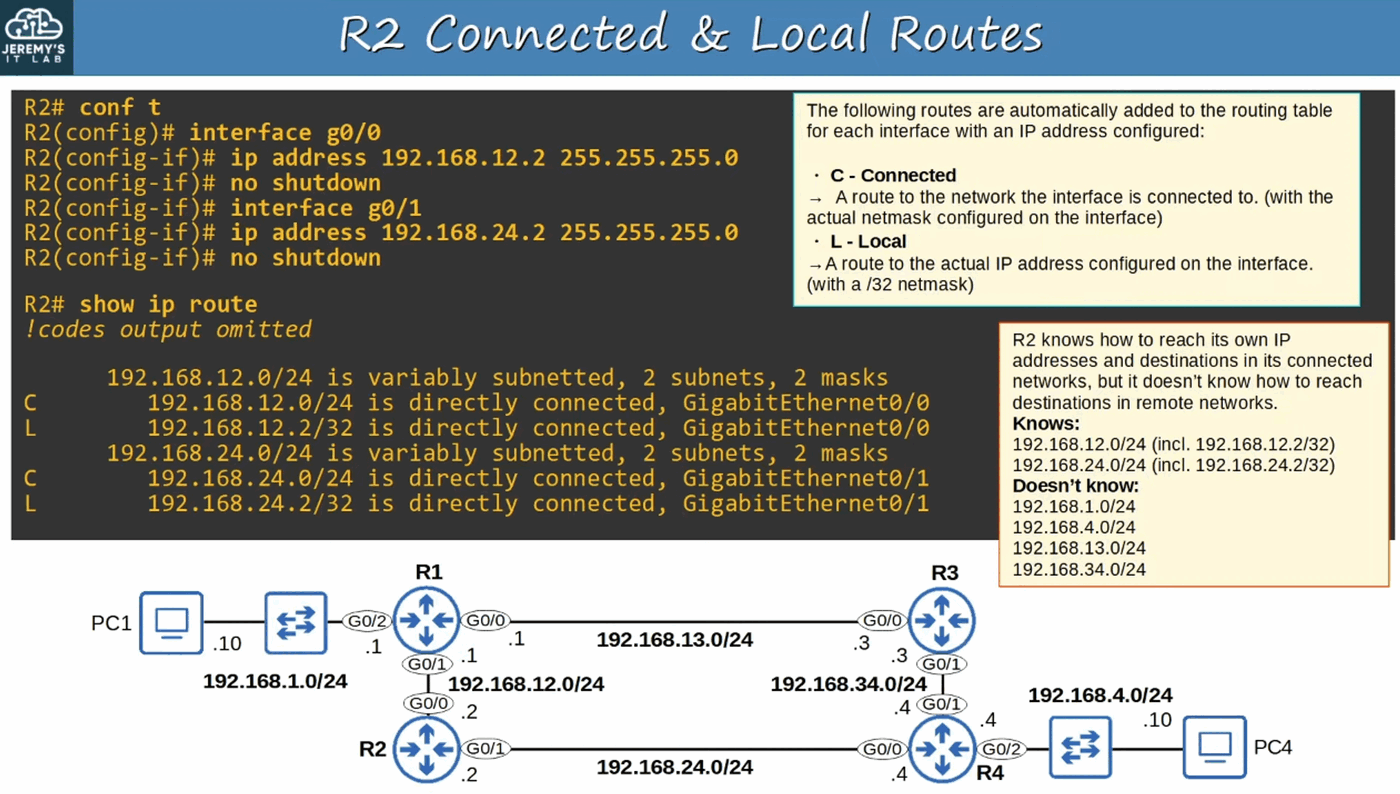
\includegraphics[keepaspectratio,alt={image}]{images/12-static-routing-part2/img-001.png}}
\end{figure}

\begin{figure}
\centering
\pandocbounded{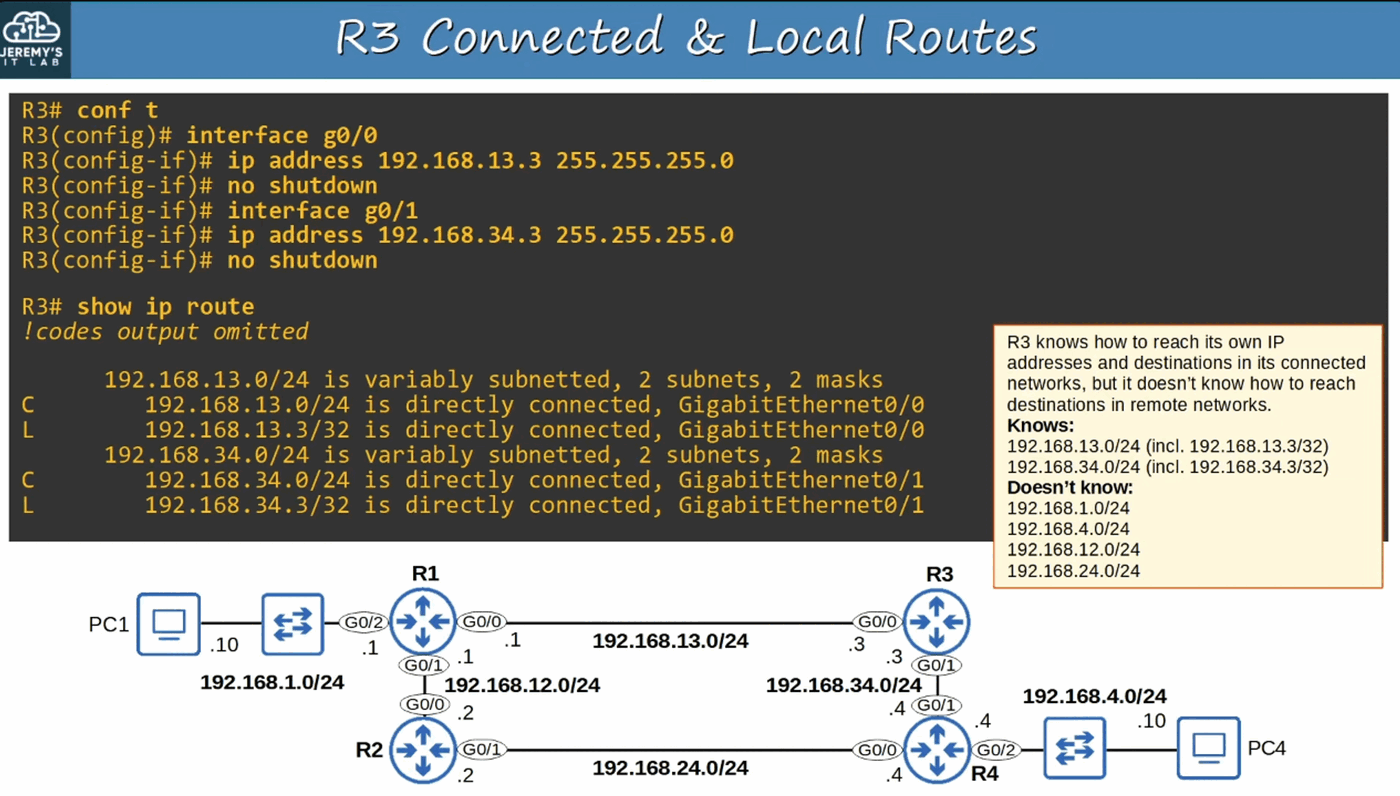
\includegraphics[keepaspectratio,alt={image}]{images/12-static-routing-part2/img-002.png}}
\end{figure}

\begin{figure}
\centering
\pandocbounded{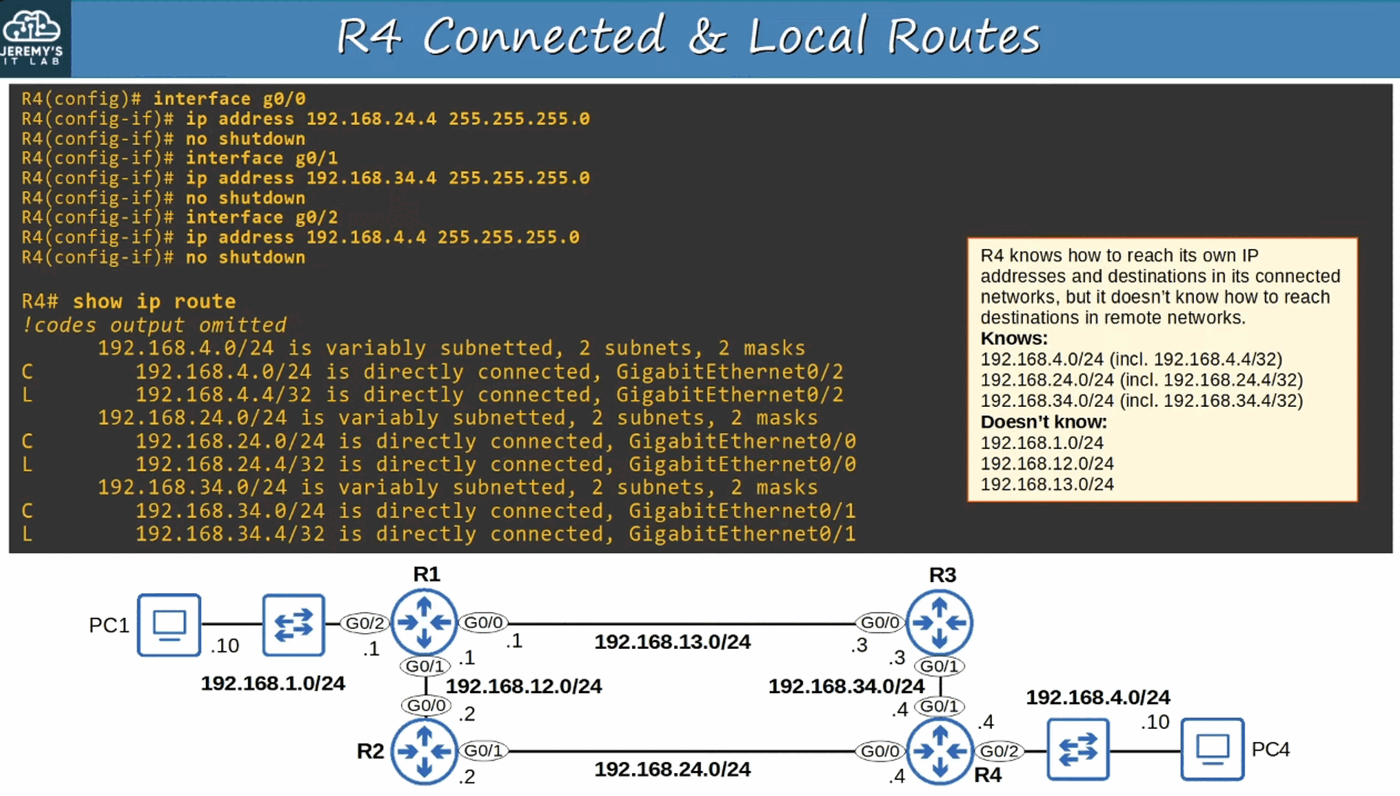
\includegraphics[keepaspectratio,alt={image}]{images/12-static-routing-part2/img-003.png}}
\end{figure}

\begin{figure}
\centering
\pandocbounded{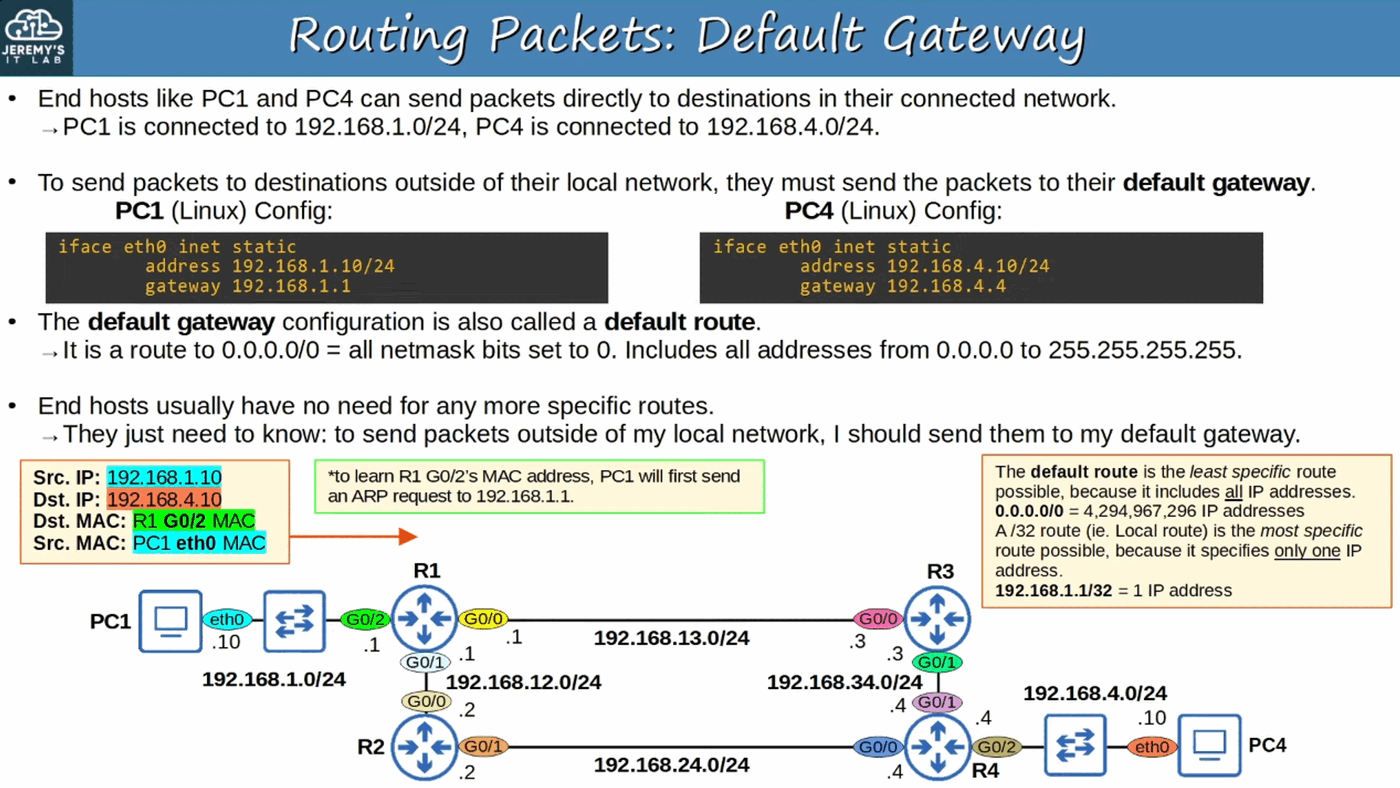
\includegraphics[keepaspectratio,alt={image}]{images/12-static-routing-part2/img-004.png}}
\end{figure}

\section{Static Routes}\label{static-routes}

\begin{figure}
\centering
\pandocbounded{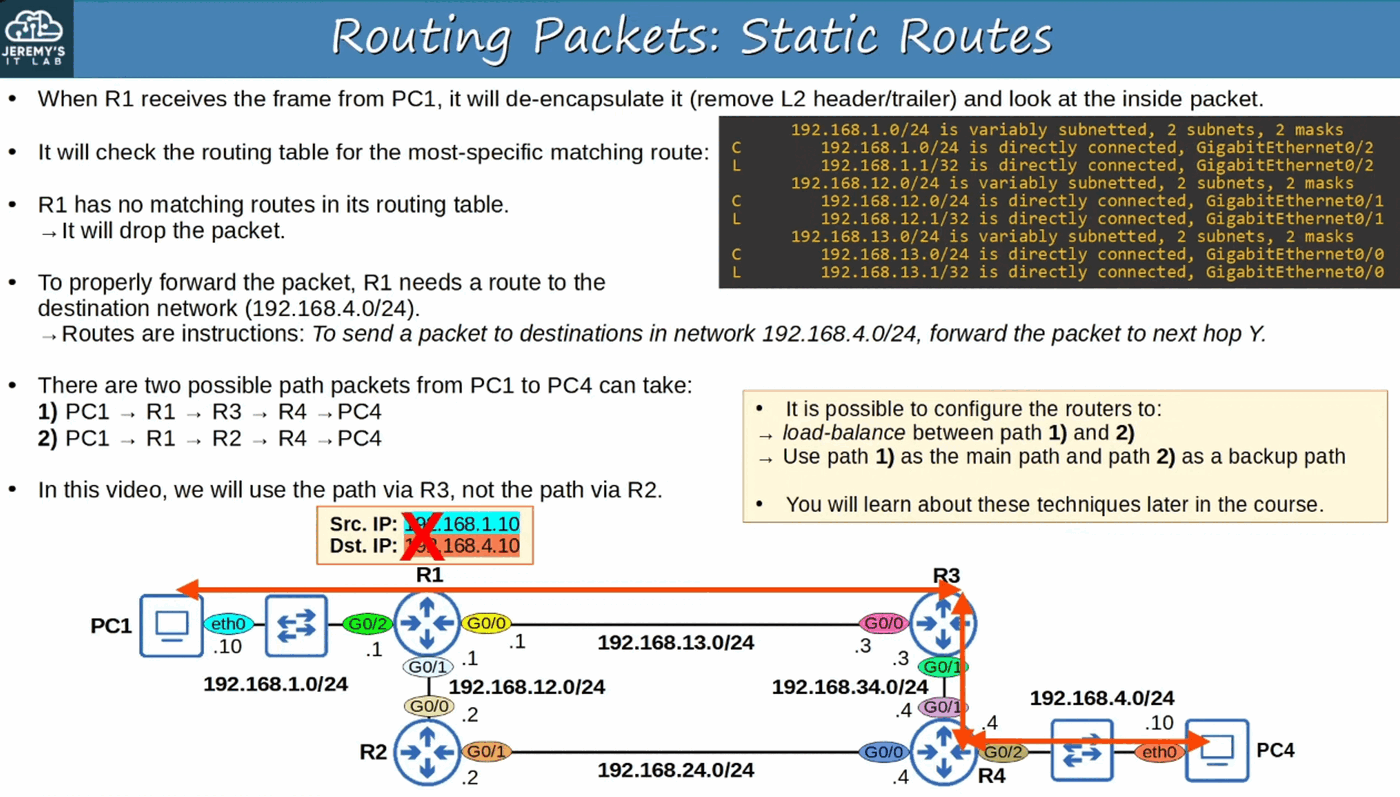
\includegraphics[keepaspectratio,alt={image}]{images/12-static-routing-part2/img-005.png}}
\end{figure}

\section{Static Route Configuration}\label{static-route-configuration}

\begin{figure}
\centering
\pandocbounded{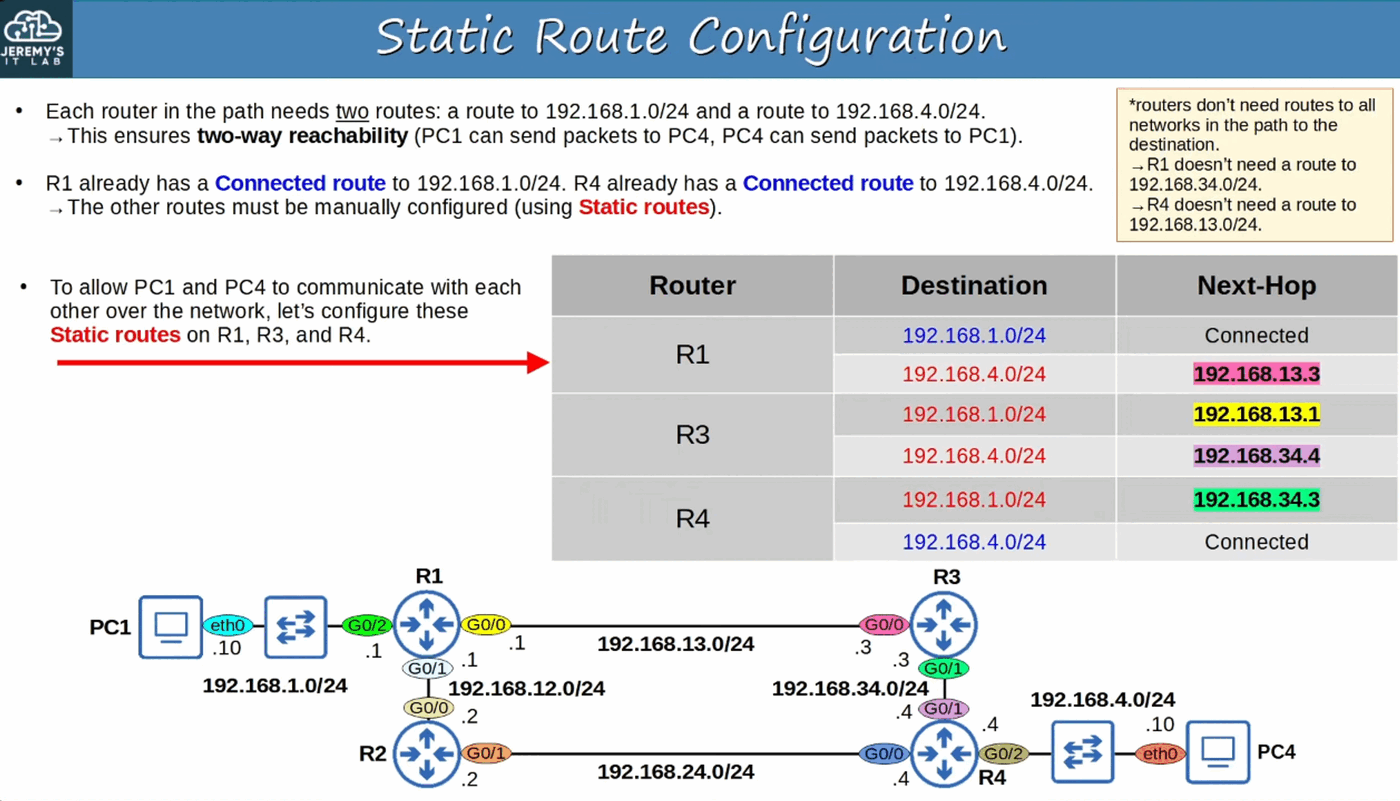
\includegraphics[keepaspectratio,alt={image}]{images/12-static-routing-part2/img-006.png}}
\end{figure}

\begin{figure}
\centering
\pandocbounded{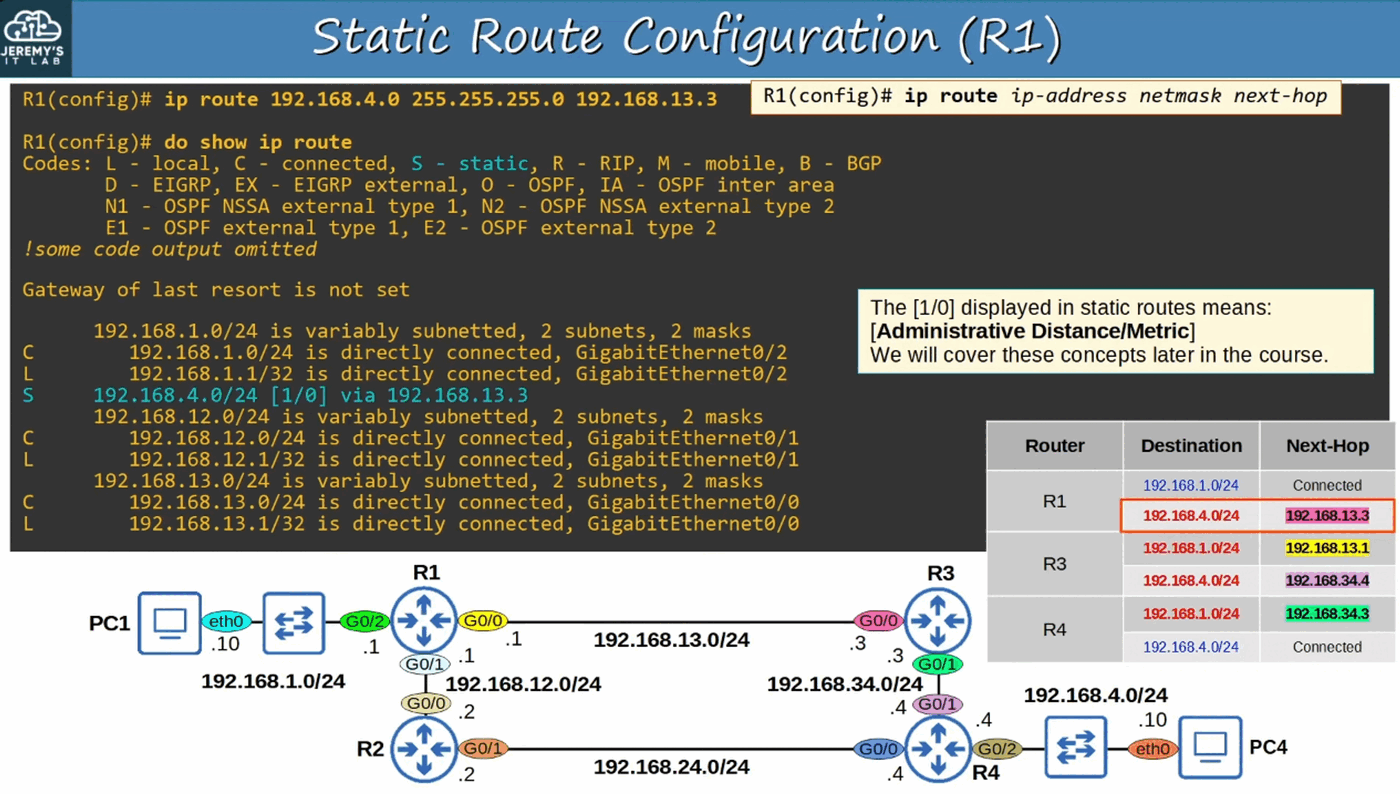
\includegraphics[keepaspectratio,alt={image}]{images/12-static-routing-part2/img-007.png}}
\end{figure}

\begin{figure}
\centering
\pandocbounded{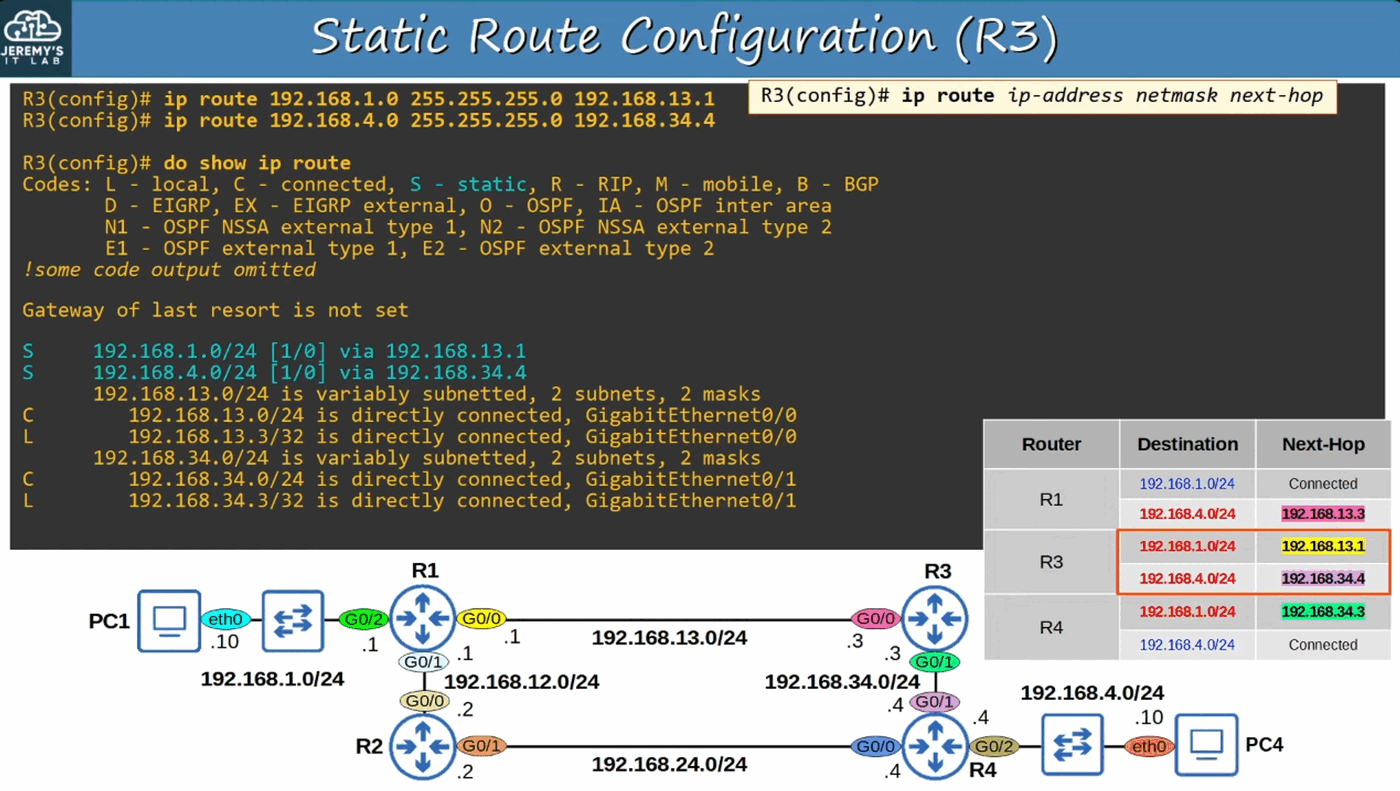
\includegraphics[keepaspectratio,alt={image}]{images/12-static-routing-part2/img-008.png}}
\end{figure}

\begin{figure}
\centering
\pandocbounded{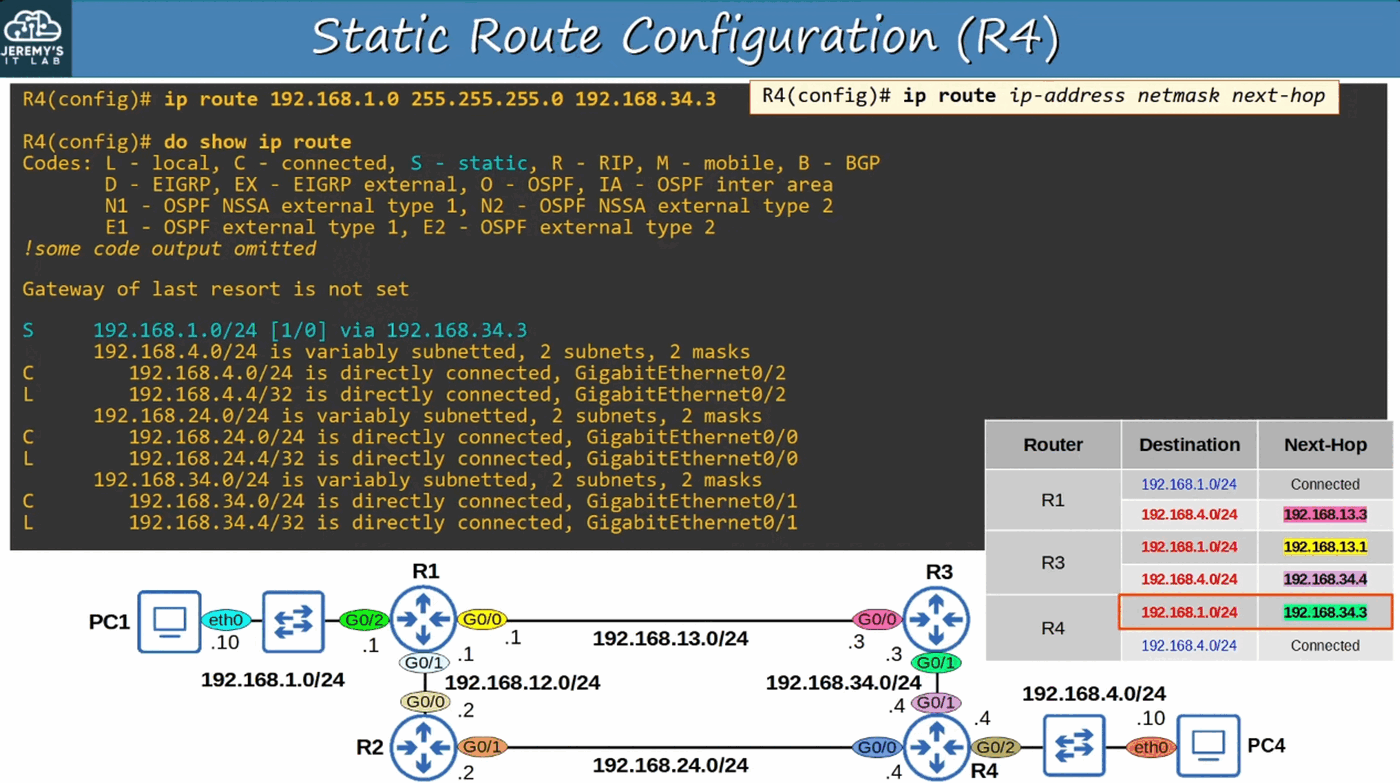
\includegraphics[keepaspectratio,alt={image}]{images/12-static-routing-part2/img-009.png}}
\end{figure}

\begin{figure}
\centering
\pandocbounded{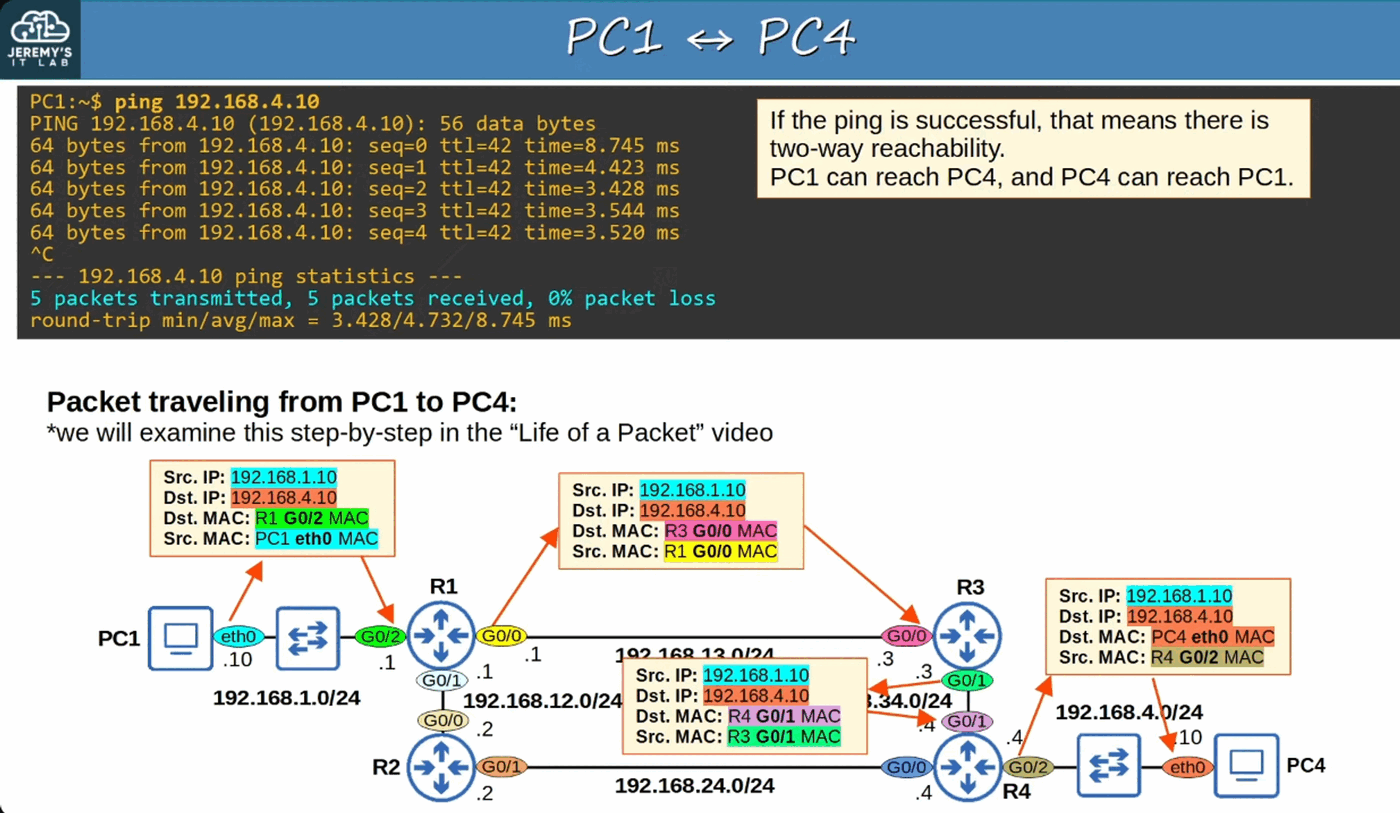
\includegraphics[keepaspectratio,alt={image}]{images/12-static-routing-part2/img-010.png}}
\end{figure}

STATIC ROUTE CONFIGURATION with \emph{exit-interface}

\begin{figure}
\centering
\pandocbounded{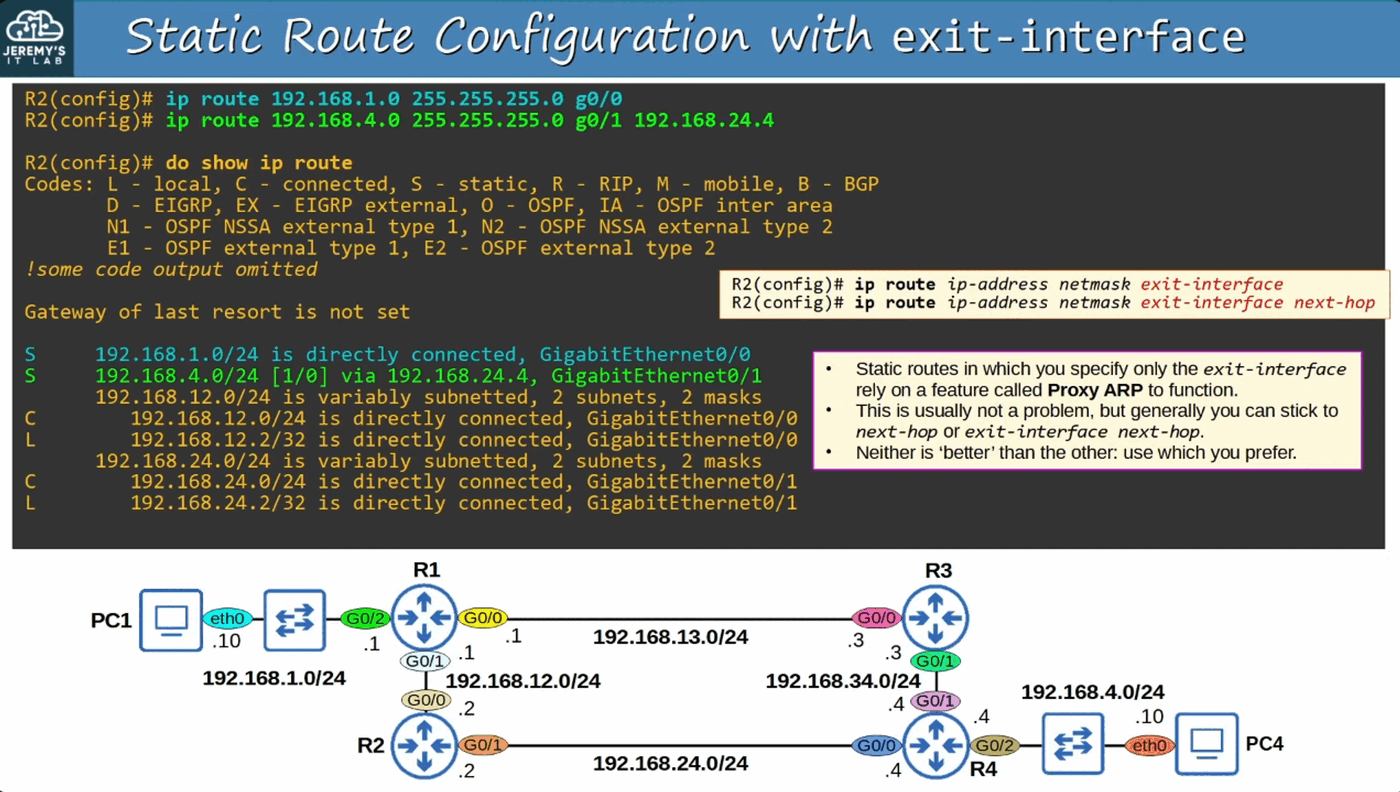
\includegraphics[keepaspectratio,alt={image}]{images/12-static-routing-part2/img-011.png}}
\end{figure}

\section{Default Route}\label{default-route}

\begin{figure}
\centering
\pandocbounded{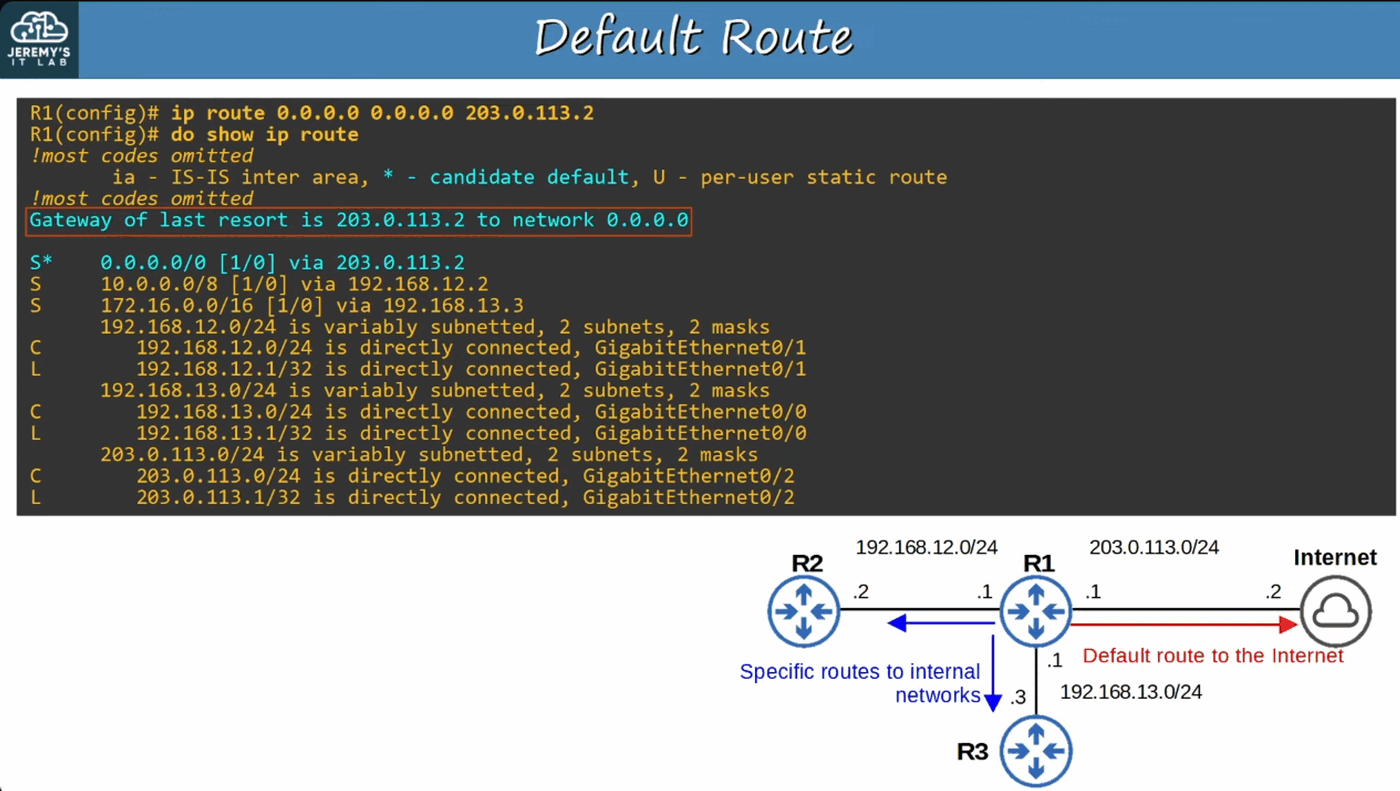
\includegraphics[keepaspectratio,alt={image}]{images/12-static-routing-part2/img-012.png}}
\end{figure}

\chapter{Life of a Packet}\label{life-of-a-packet}

\begin{figure}
\centering
\pandocbounded{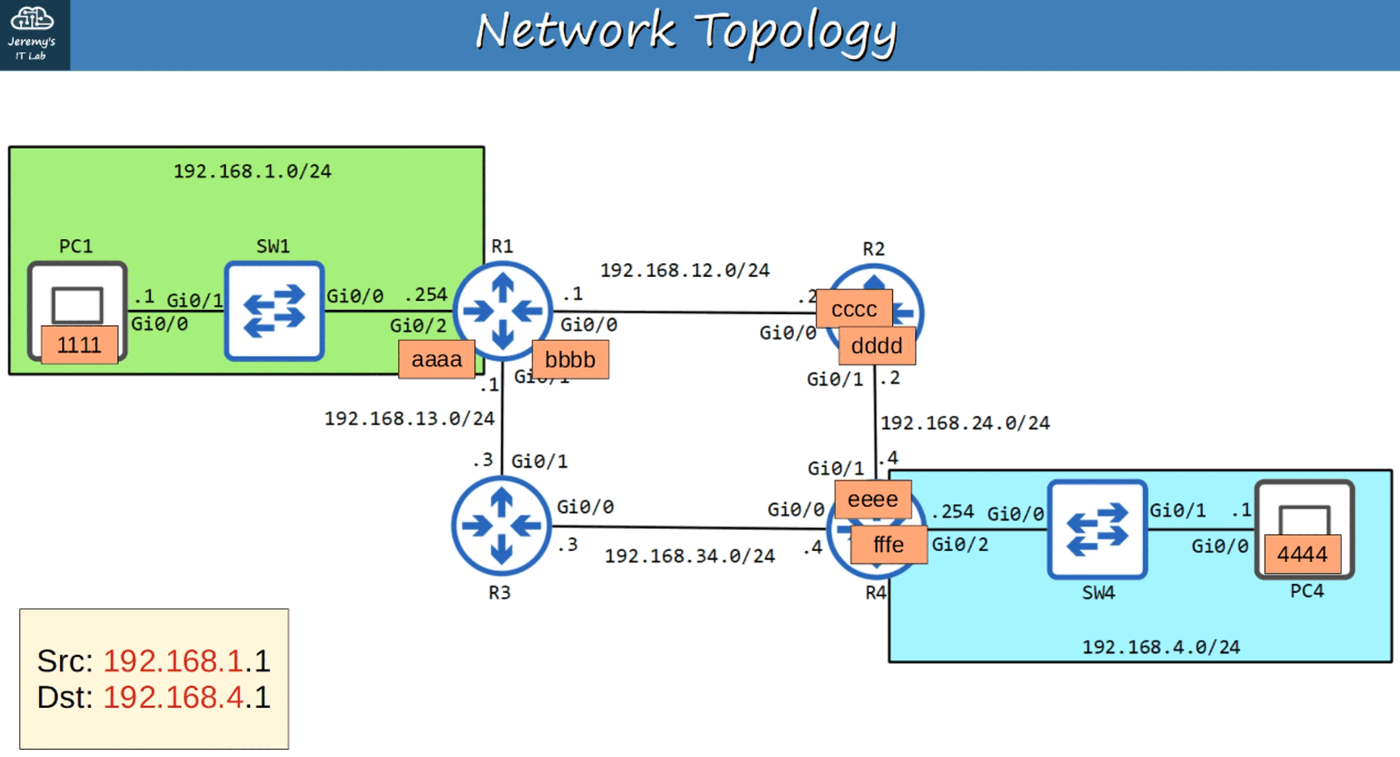
\includegraphics[keepaspectratio,alt={image}]{images/13-life-of-a-packet/img-001.png}}
\end{figure}

EACH Network device's interfaces have a UNIQUE MAC Addresses.

In a TCP HEADER

SOURCE IP ADDRESS comes before DESTINATION IP ADDRESS

while\ldots{}

in an ETHERNET HEADER

DESTINATION MAC ADDRESS comes before SOURCE MAC ADDRESS

\begin{figure}
\centering
\pandocbounded{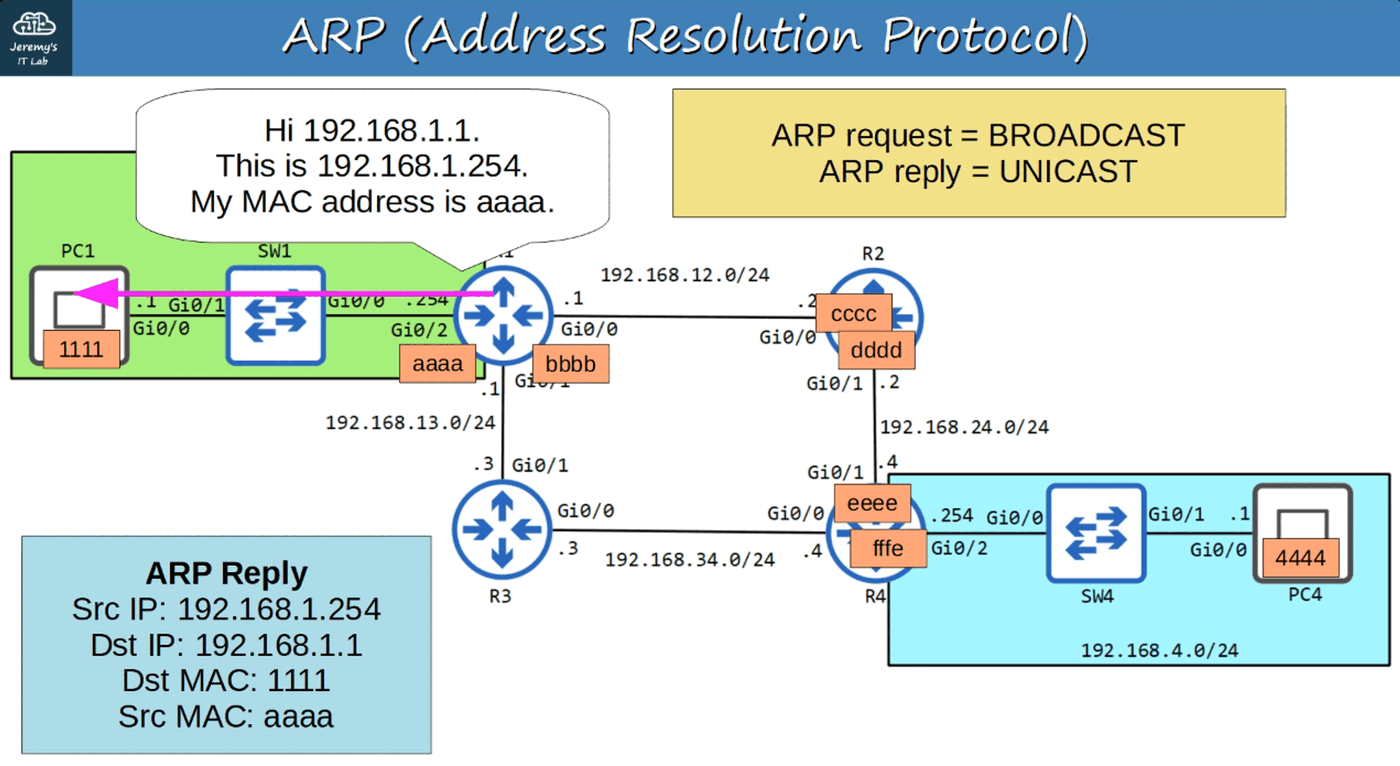
\includegraphics[keepaspectratio,alt={image}]{images/13-life-of-a-packet/img-002.png}}
\end{figure}

\begin{figure}
\centering
\pandocbounded{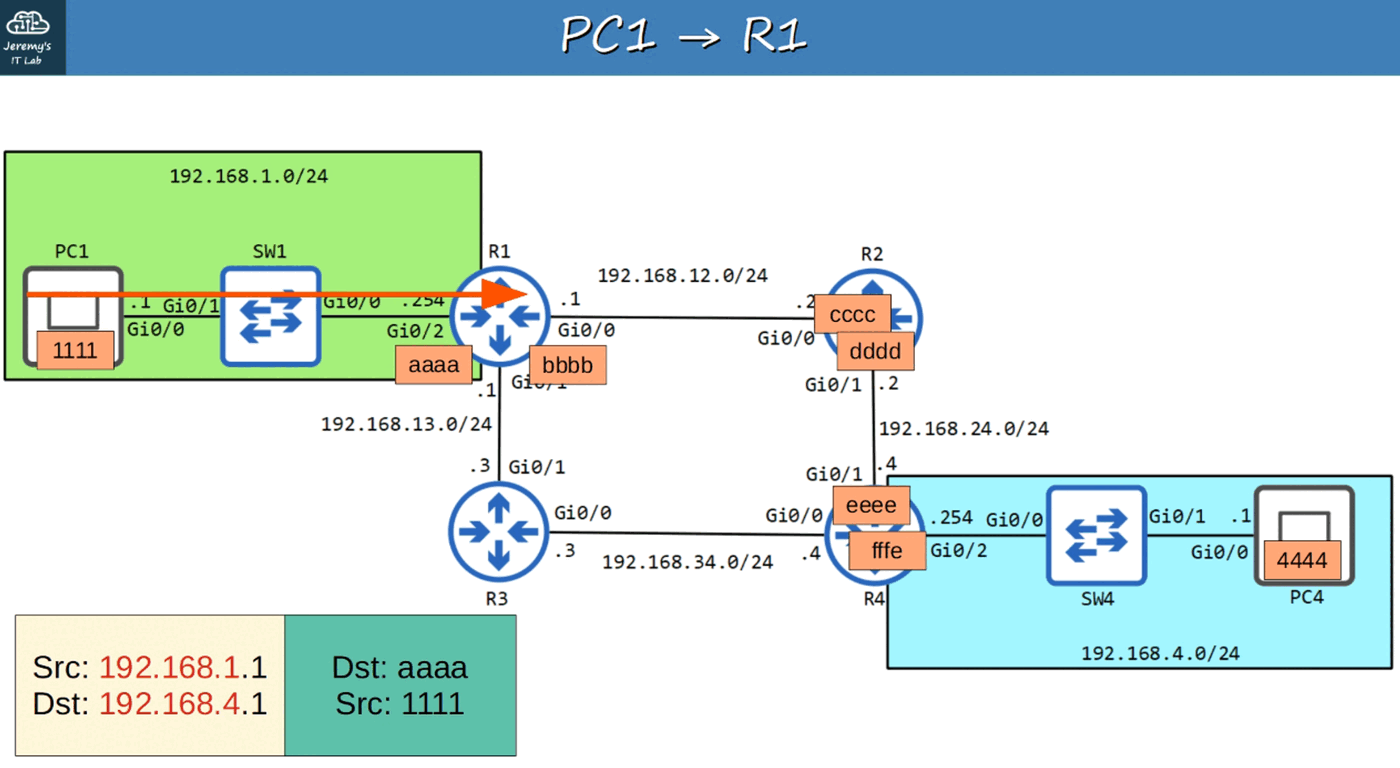
\includegraphics[keepaspectratio,alt={image}]{images/13-life-of-a-packet/img-003.png}}
\end{figure}

\begin{figure}
\centering
\pandocbounded{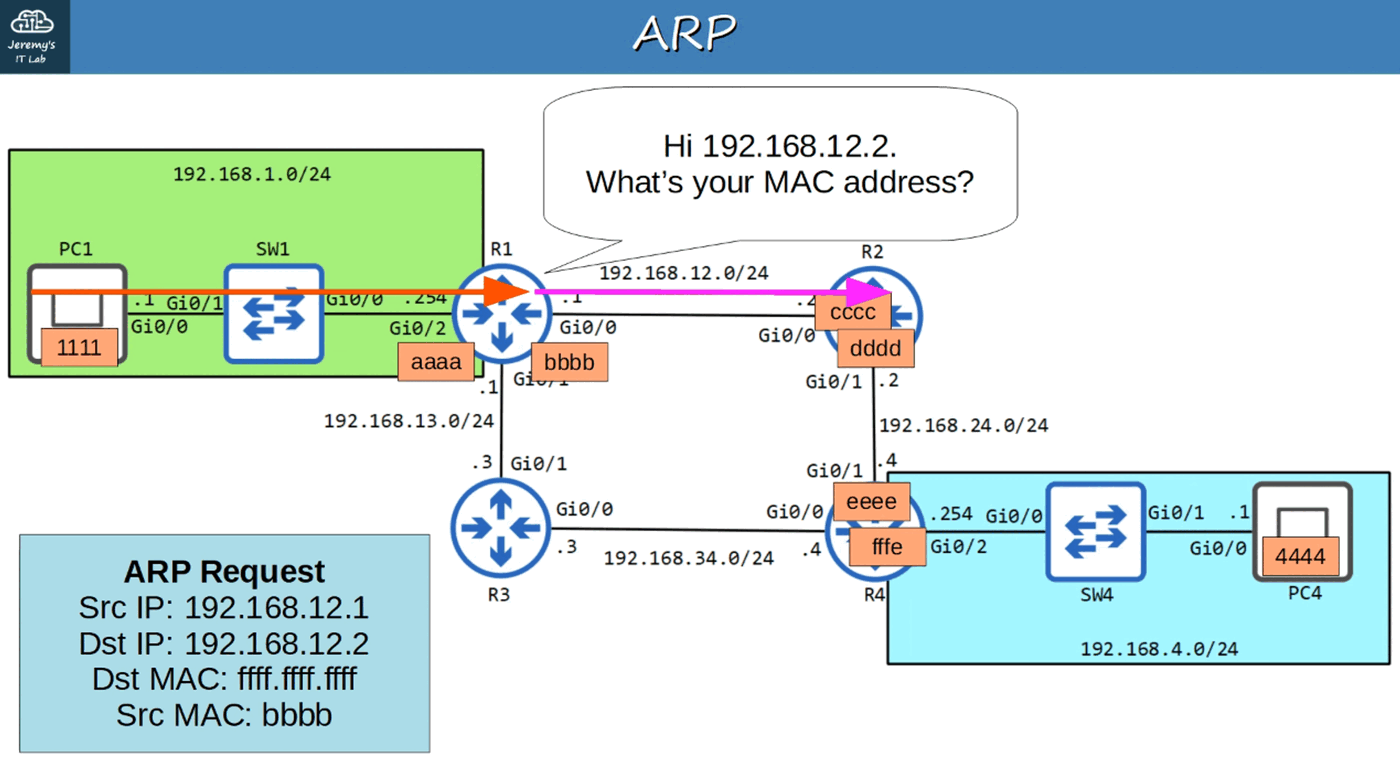
\includegraphics[keepaspectratio,alt={image}]{images/13-life-of-a-packet/img-004.png}}
\end{figure}

\begin{figure}
\centering
\pandocbounded{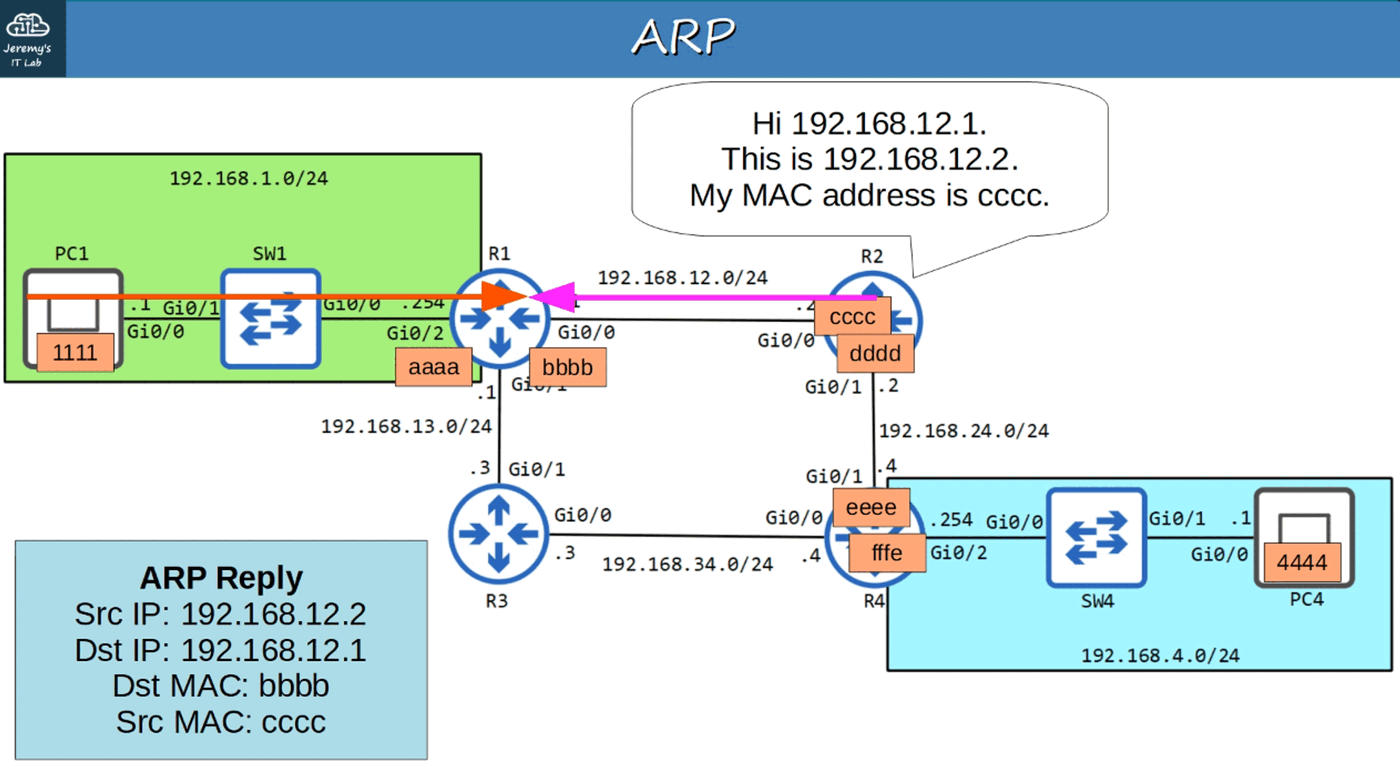
\includegraphics[keepaspectratio,alt={image}]{images/13-life-of-a-packet/img-005.png}}
\end{figure}

\begin{figure}
\centering
\pandocbounded{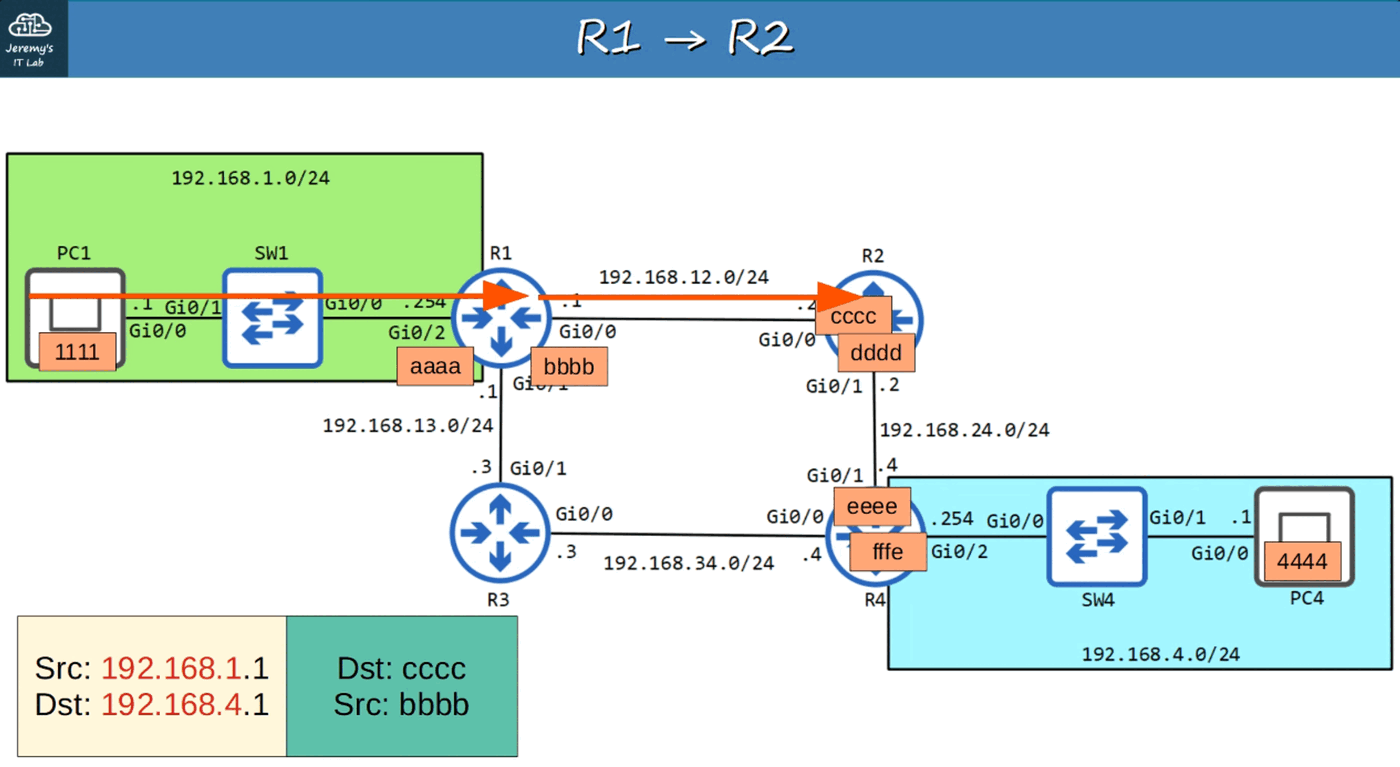
\includegraphics[keepaspectratio,alt={image}]{images/13-life-of-a-packet/img-006.png}}
\end{figure}

\begin{figure}
\centering
\pandocbounded{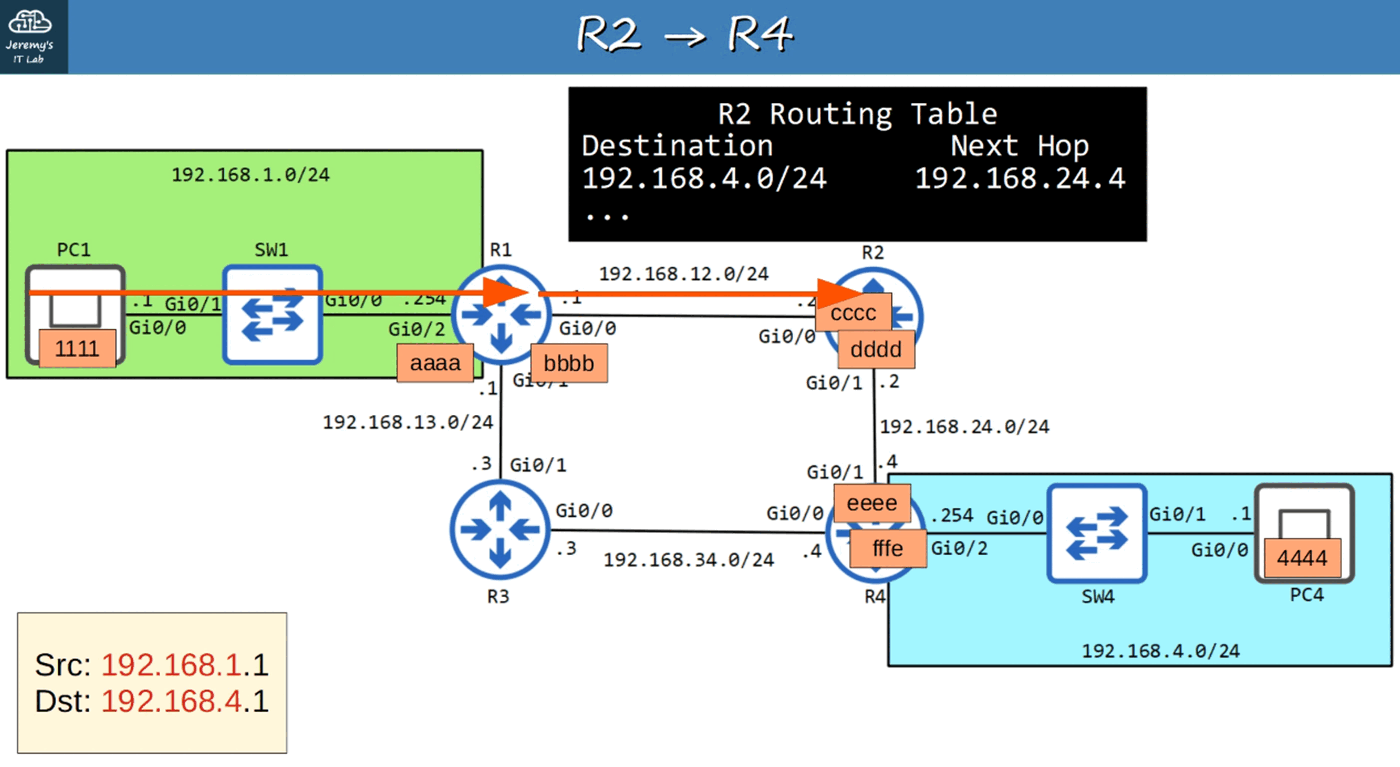
\includegraphics[keepaspectratio,alt={image}]{images/13-life-of-a-packet/img-007.png}}
\end{figure}

\begin{figure}
\centering
\pandocbounded{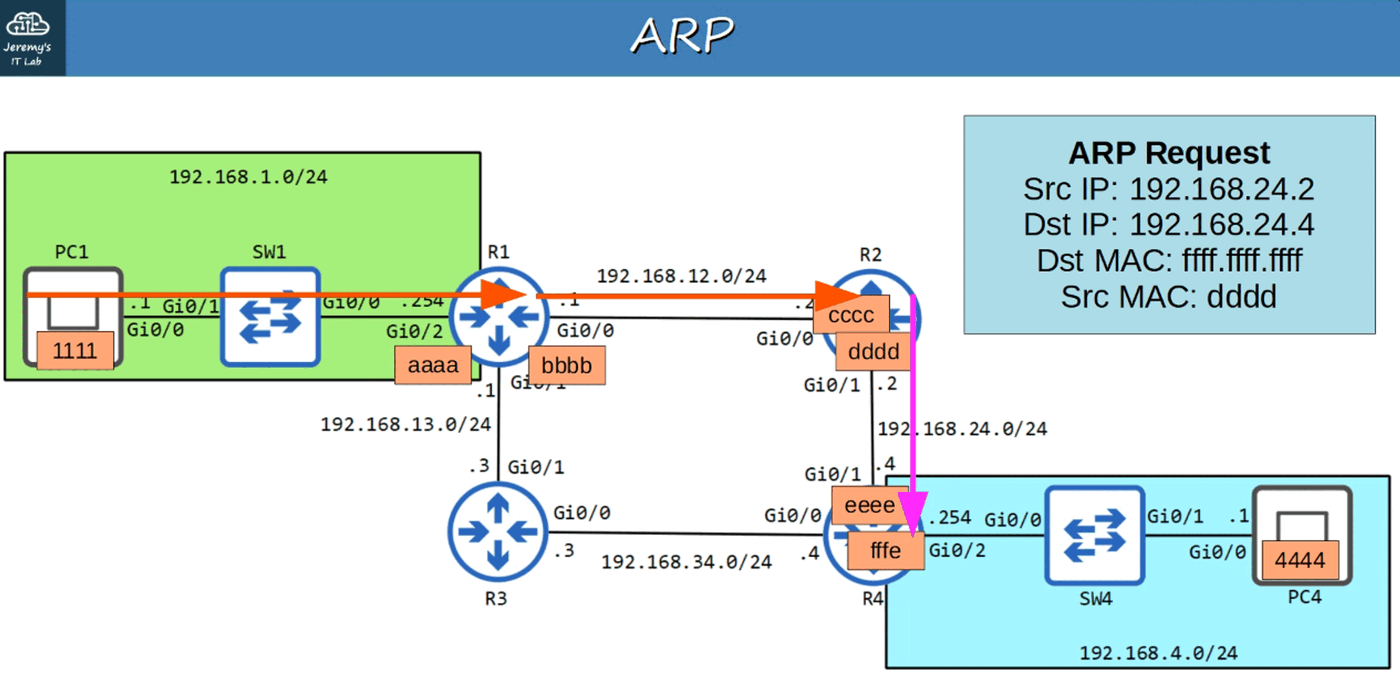
\includegraphics[keepaspectratio,alt={image}]{images/13-life-of-a-packet/img-008.png}}
\end{figure}

\begin{figure}
\centering
\pandocbounded{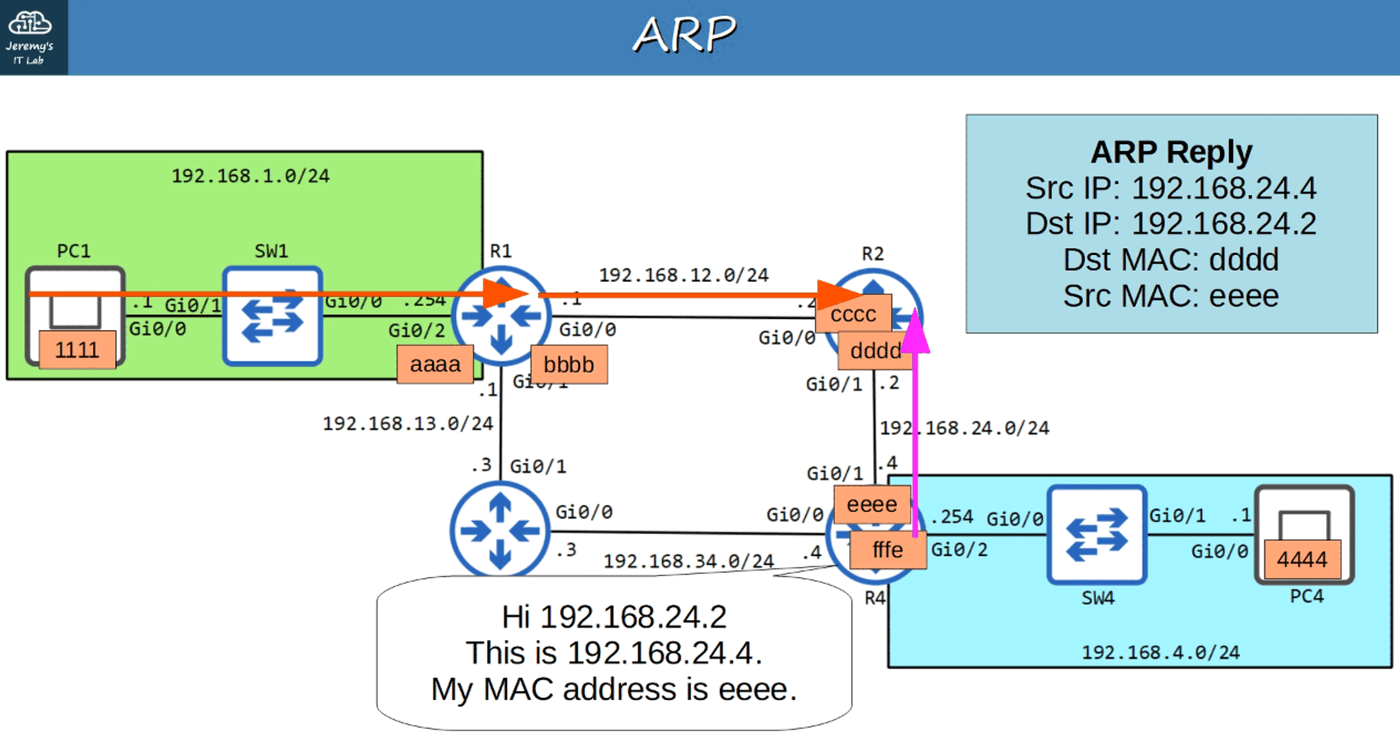
\includegraphics[keepaspectratio,alt={image}]{images/13-life-of-a-packet/img-009.png}}
\end{figure}

\begin{figure}
\centering
\pandocbounded{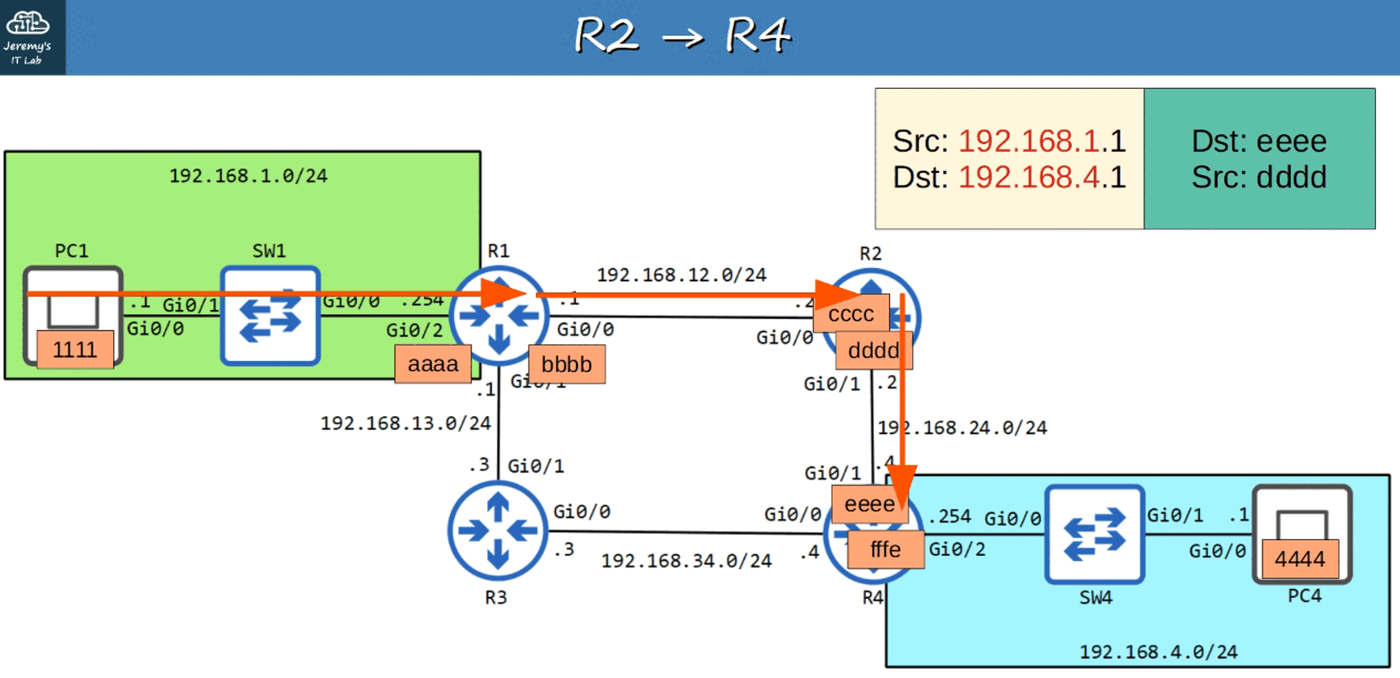
\includegraphics[keepaspectratio,alt={image}]{images/13-life-of-a-packet/img-010.png}}
\end{figure}

\begin{figure}
\centering
\pandocbounded{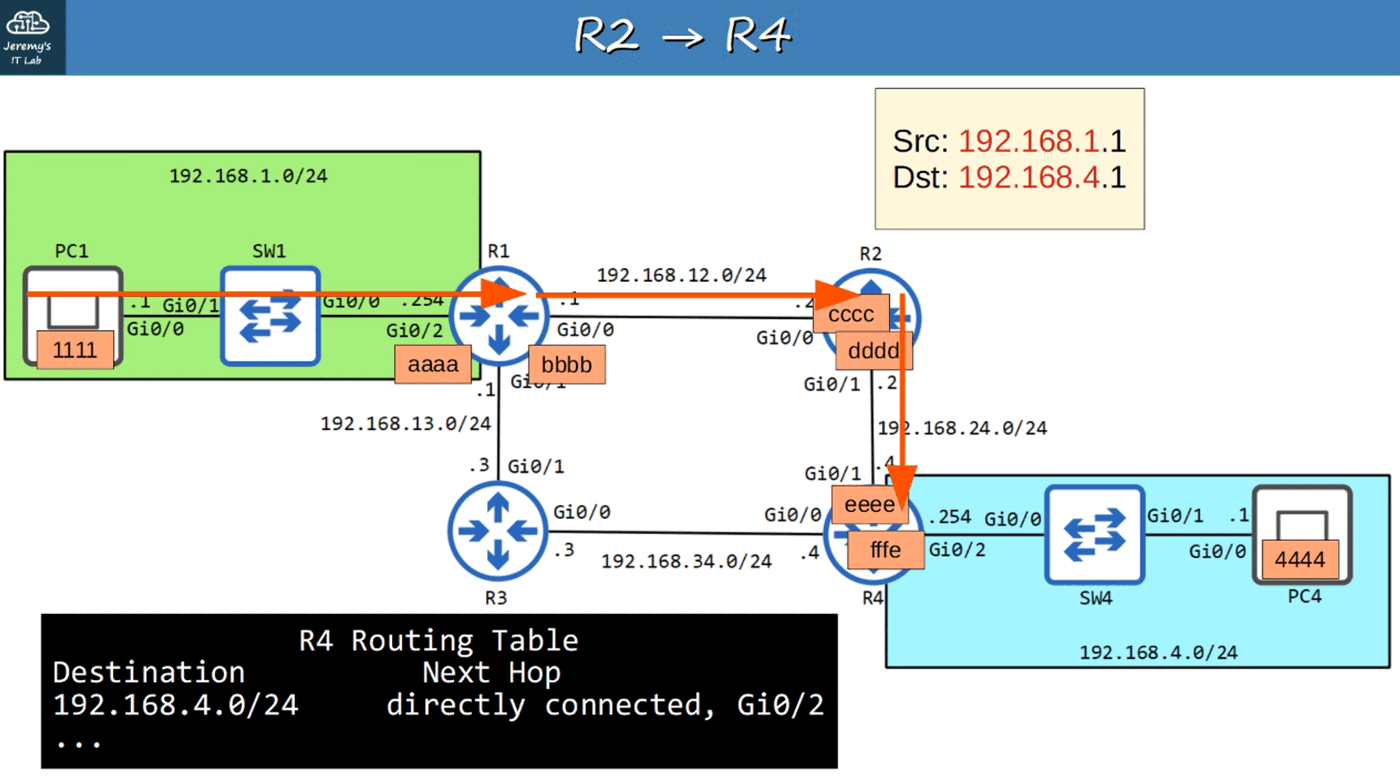
\includegraphics[keepaspectratio,alt={image}]{images/13-life-of-a-packet/img-011.png}}
\end{figure}

\begin{figure}
\centering
\pandocbounded{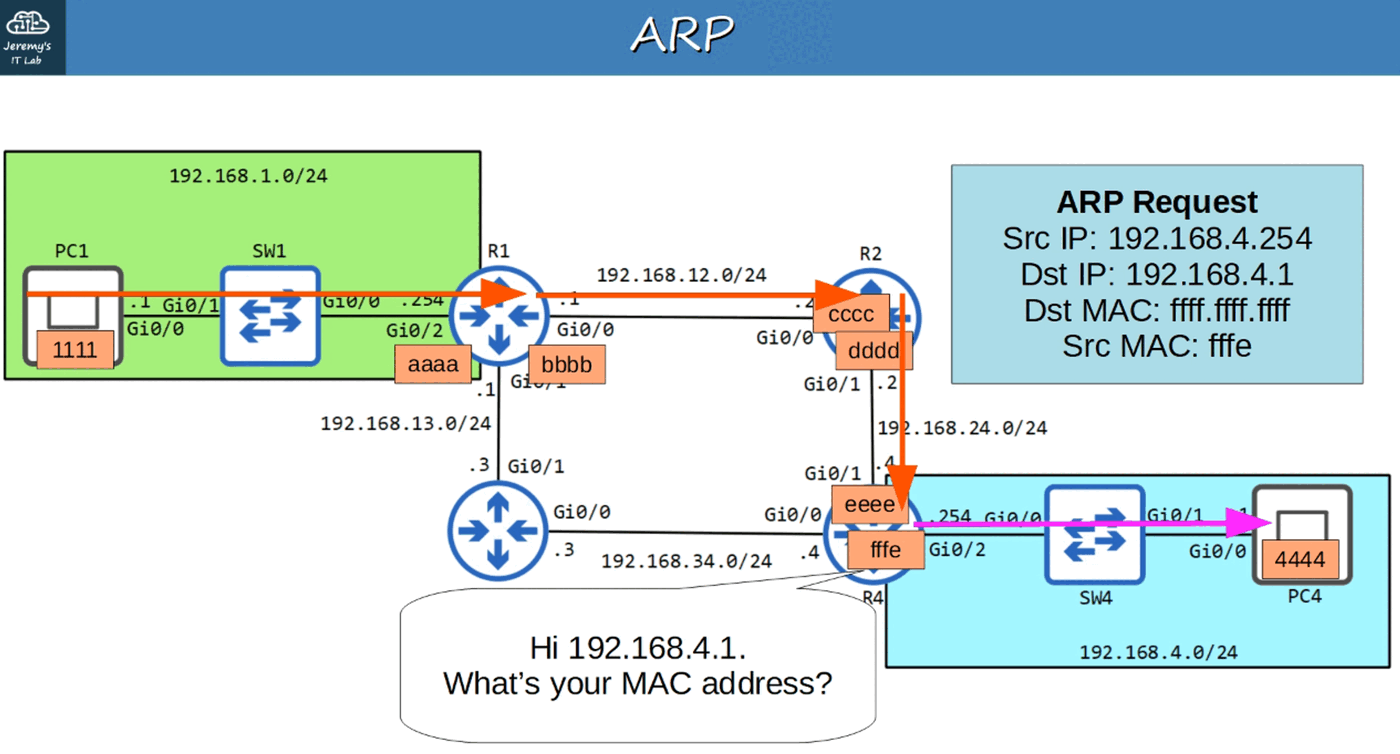
\includegraphics[keepaspectratio,alt={image}]{images/13-life-of-a-packet/img-012.png}}
\end{figure}

\begin{figure}
\centering
\pandocbounded{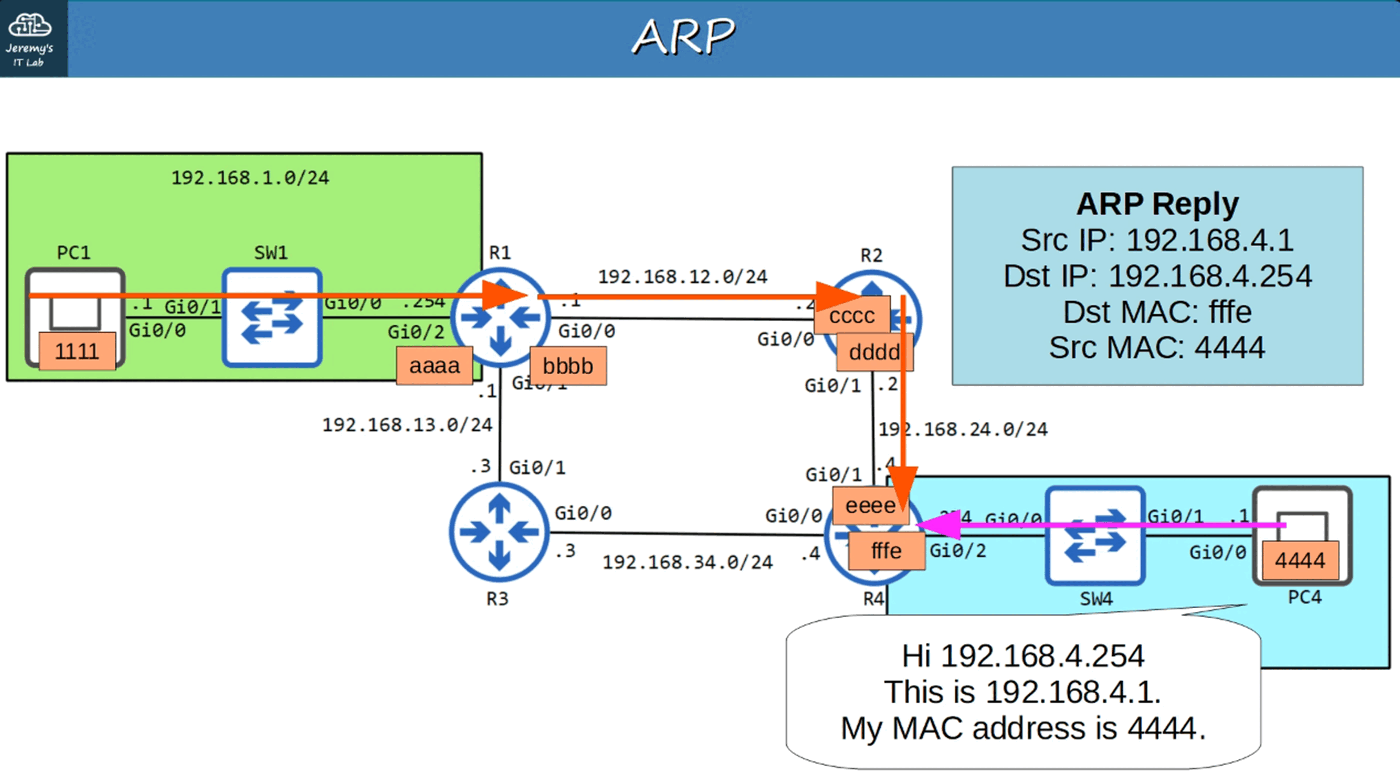
\includegraphics[keepaspectratio,alt={image}]{images/13-life-of-a-packet/img-013.png}}
\end{figure}

\begin{figure}
\centering
\pandocbounded{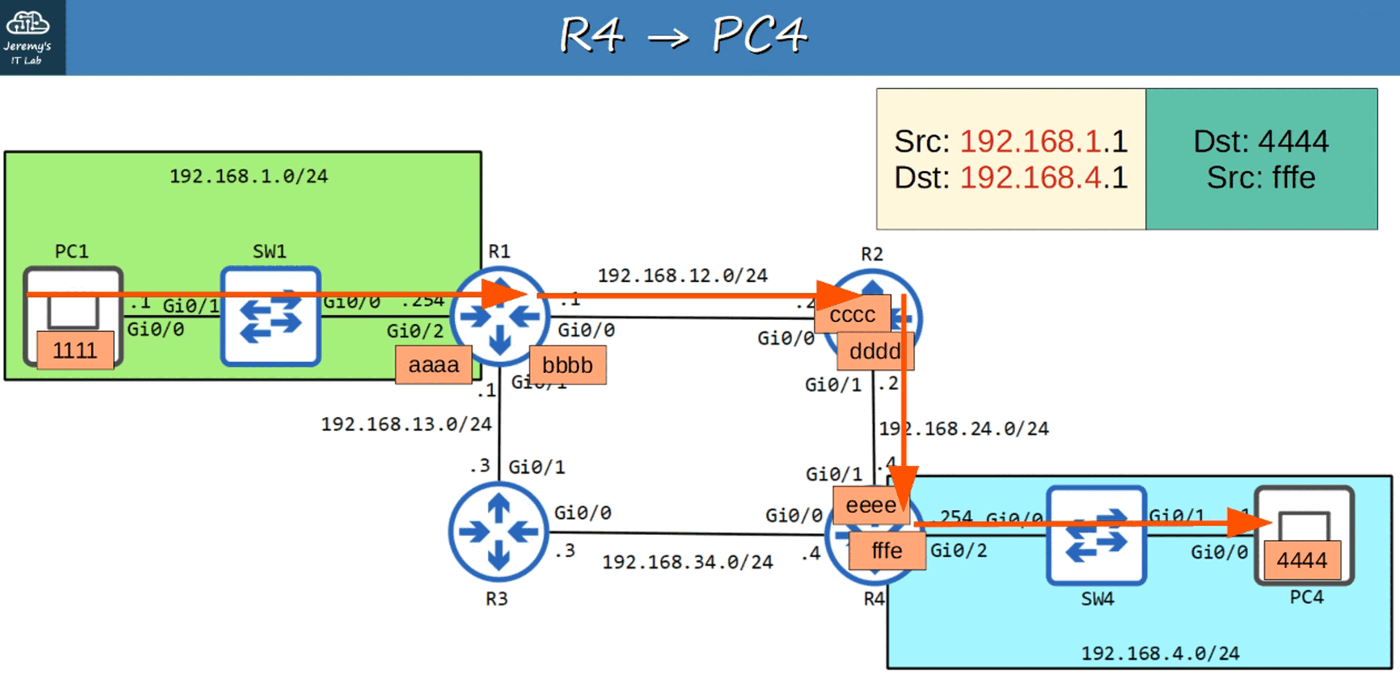
\includegraphics[keepaspectratio,alt={image}]{images/13-life-of-a-packet/img-014.png}}
\end{figure}

\begin{figure}
\centering
\pandocbounded{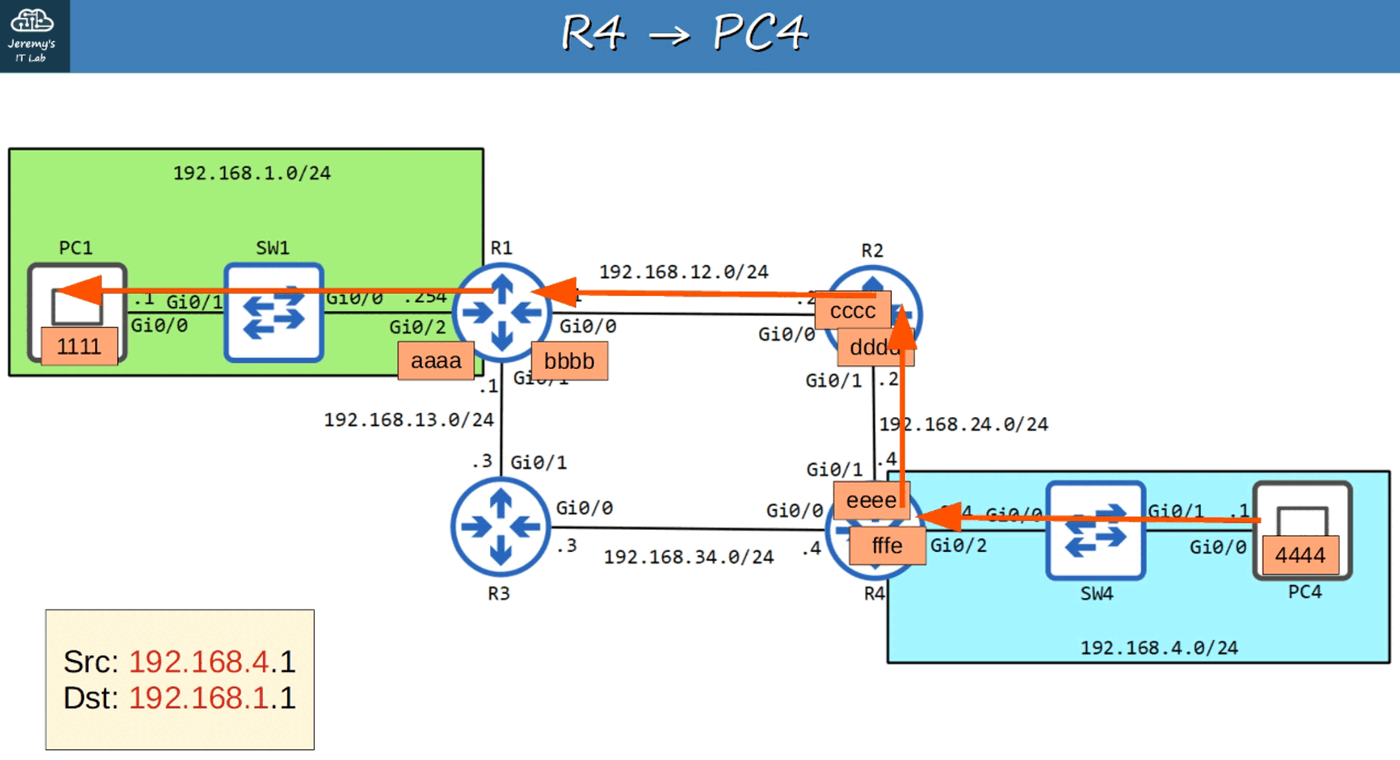
\includegraphics[keepaspectratio,alt={image}]{images/13-life-of-a-packet/img-015.png}}
\end{figure}

When a HOST sends a packet to another HOST, the SOURCE or DESTINATION IP
doesn't change - even though ROUTERS may change the ETHERNET HEADER
(SRC/DEST MAC ADDRESSES).

\chapter{Subnetting: Part 1}\label{subnetting-part-1}

\begin{figure}
\centering
\pandocbounded{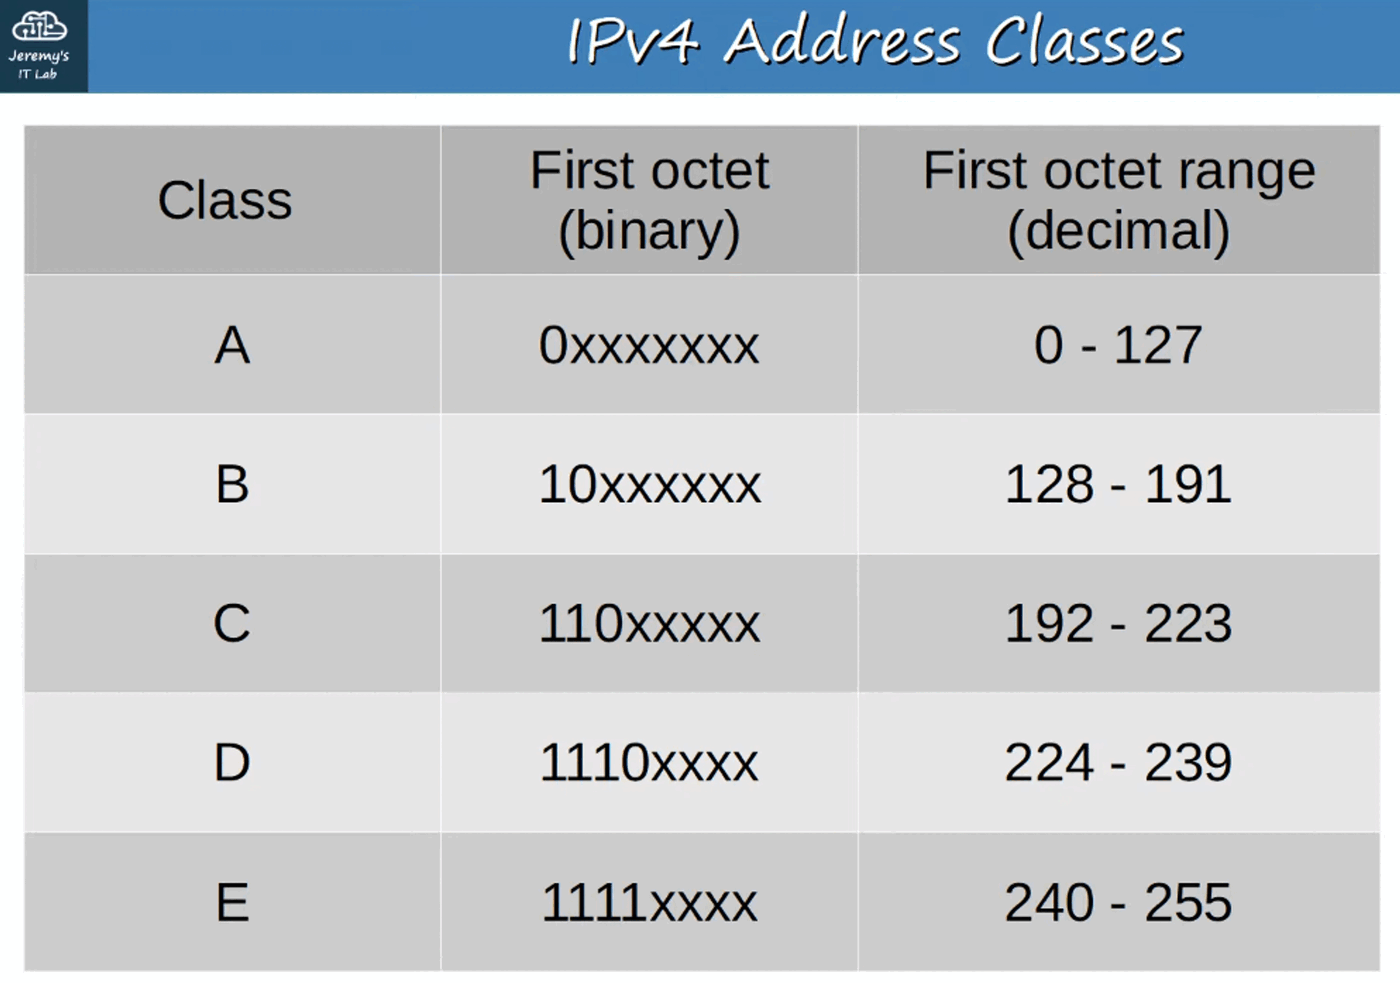
\includegraphics[keepaspectratio,alt={image}]{images/14-subnetting-part1/img-001.png}}
\end{figure}

HOWEVER, only Class A, B, C Addresses can be assigned to a device as an
IP Address.

\begin{lstlisting}
CLASS       PREFIX LENGTH

A           /8
B           /16
C           /24
\end{lstlisting}

\begin{figure}
\centering
\pandocbounded{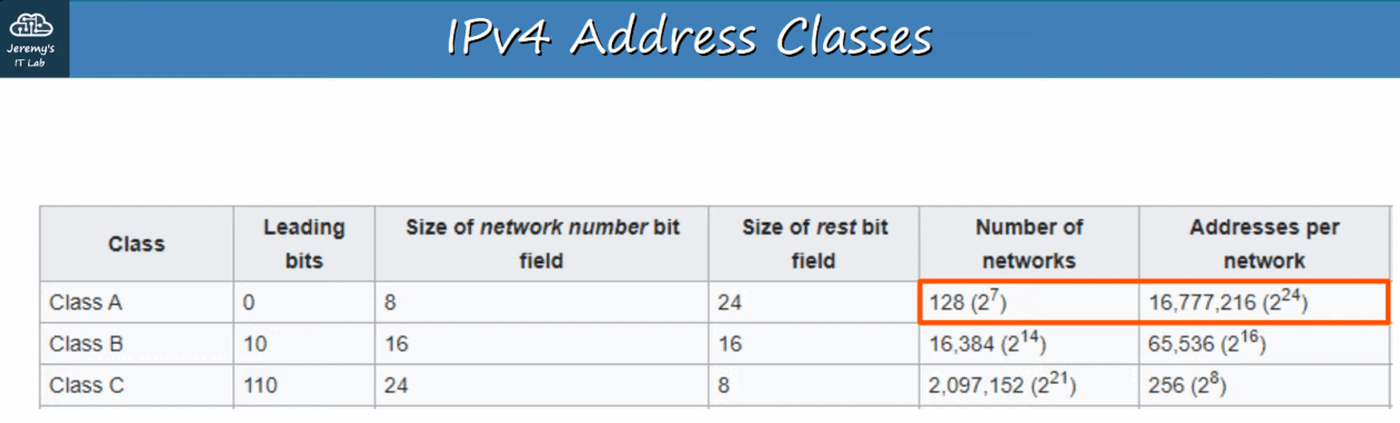
\includegraphics[keepaspectratio,alt={image}]{images/14-subnetting-part1/img-002.png}}
\end{figure}

The IANA (Internet Assigned Numbers Authority) assigns IPv4
addresses/networks to companies based on their size.

The problem with `CLASSFUL' assignment is that it led to IP Address
wastefulness.

Example: A company requiring 5000 address was assigned a CLASS B IP,
leaving 60000+ addresses unused.

The IETF (Internet Engineering Task Force) introduce CIDR in 1993 to
replace the ``classful'' addressing system.

CIDR (Classless Inter-Domain Routing) removed the requirements of CLASS
A, B, and C regarding size.

\begin{itemize}
\tightlist
\item
  This allowed larger networks to be split into smaller networks,
  allowing greater efficiency.
\item
  These smaller networks are called ``SUB-NETWORKS'' or ``SUBNETS''
\end{itemize}

HOW MANY USABLE ADDRESSES ARE THERE IN EACH NETWORK?

\section{Remember}\label{remember}

2\^{}n - 2 = Usable Address n = number of host bits

CIDR PRACTICE!

203.0.113.0/25

/25 means the Subnetwork bit is 25 bits

203 . 0 . 113 . 0 is written in binary as :

1100 1011 . 0000 0000 . 0111 0001 . 0 \textbar{} 000 0000

(Subnet prefix is the first 25 bits)

Flipping all the bits to 1's, we get the SUBNET MASK for /25:

1111 1111 . 1111 1111 . 1111 1111 . 1 \textbar{} 000 0000

which is equal to:

255.255.255.128 (because the last octet is 1000 0000 = 128 in binary)

SO - the based on previous definition of USABLE ADDRESSES, the number of
hosts for 203.0.113.0 /25 is:

2\^{}(7 bits) or (128) - 2 = 126 hosts.

What about /28 ?

203 . 0 . 113 . 0 is written in binary as :

1100 1011 . 0000 0000 . 0111 0001 . 0000 \textbar{} 0000

(Subnet prefix is the first 28 bits)

flipping all the bits to 1's, we get the SUBNET MASK for /28:

1111 1111 . 1111 1111 . 1111 1111 . 1111 \textbar{} 0000

which is equal to:

255.255.255.240 (because the last octet is 1111 0000) = 128+64+32+16 =
(128+32) + (64+16) = 160 + 80 = 240

The SUBNET MASK for /28 is 255.255.255.240 which has 16 hosts / group (2
* 4 bits = 16) - 2 Reserved IPs for Network and Broadcast

\section{Subnetting Cheatsheet}\label{subnetting-cheatsheet}

{\def\LTcaptype{none} % do not increment counter
\begin{longtable}[]{@{}lllllllll@{}}
\toprule\noalign{}
Group Size & 128 & 64 & 32 & 16 & 8 & 4 & 2 & 1 \\
\midrule\noalign{}
\endhead
\bottomrule\noalign{}
\endlastfoot
Subnet Mask & 128 & 192 & 224 & 240 & 248 & 252 & 254 & 255 \\
CIDR & /25 & /26 & /27 & /28 & /29 & /30 & /31 & /32 \\
3rd Octet & /17 & /18 & /19 & /20 & /21 & /22 & /23 & /24 \\
2nd Octet & /9 & /10 & /11 & /12 & /13 & /14 & /15 & /16 \\
1st Octet & /1 & /2 & /3 & /4 & /5 & /6 & /7 & /8 \\
\end{longtable}
}

\begin{enumerate}
\def\labelenumi{\arabic{enumi}.}
\item
  Use a given CIDR/Mask to find column on Cheat Sheet

  \begin{enumerate}
  \def\labelenumii{\alph{enumii})}
  \item
    CIDR/Subnet Mask map to each other
  \item
    Locate Group Size
  \item
    Increase by Group Size until you PASS the Target IP (not less or
    equal !)
  \item
    If passing the Target IP reaches 256, increase the Octet BEFORE it
    by one and current Octet becomes 0 : IF NECESSARY
  \end{enumerate}

  Example: 10.2.2.256 \(\rightarrow\) 10.2.3.0
\item
  Number BEFORE Target IP is NETWORK ID
\item
  Number AFTER Target IP is NEXT NETWORK
\item
  IP Address BEFORE Next Network is BROADCAST
\item
  IP Address AFTER Network ID is First Host
\item
  IP Address BEFORE Broadcast IP is Last Host
\item
  Group Size is total \# of IP Addresses

  \begin{itemize}
  \tightlist
  \item
    Don't forget to subtract 2 for USABLE \#
  \end{itemize}
\end{enumerate}

Solving CIDR/Subnet for 3rd Octet IPs :

Every number LEFT of 3rd Octet is 255. Every number RIGHT of 3rd Octet
is 0

Example: 10.4.77.188 / 19 \(\rightarrow\) Subnet : 255.255.224.0

You use the SAME process as above except when finding Target IPs, you
use the 3rd Octet for your Target.

Example: 10.4.77.188 /19 \(\rightarrow\) Subnet : 255.255.224.0

256 - 224 = 32 so\ldots{}

Using 32, we step through the address blocks 0, 32,64, and 96. Since 77
is between 64 and 96, there's our range.

Network: 10.4.64.0 (Start / First Block)

Next: 10.4.96.0 (Second Block) \ldots{}

Number of IP Addresses is : 2\^{}(32-CIDR). In this example 2\^{}13 =
8192

Solving for 2nd and 1st Octet is the same as above, keeping in mind the
Octet column is USED to check for the Target number of a given address.

Alternative method to ``Cheat Sheet''

\begin{figure}
\centering
\pandocbounded{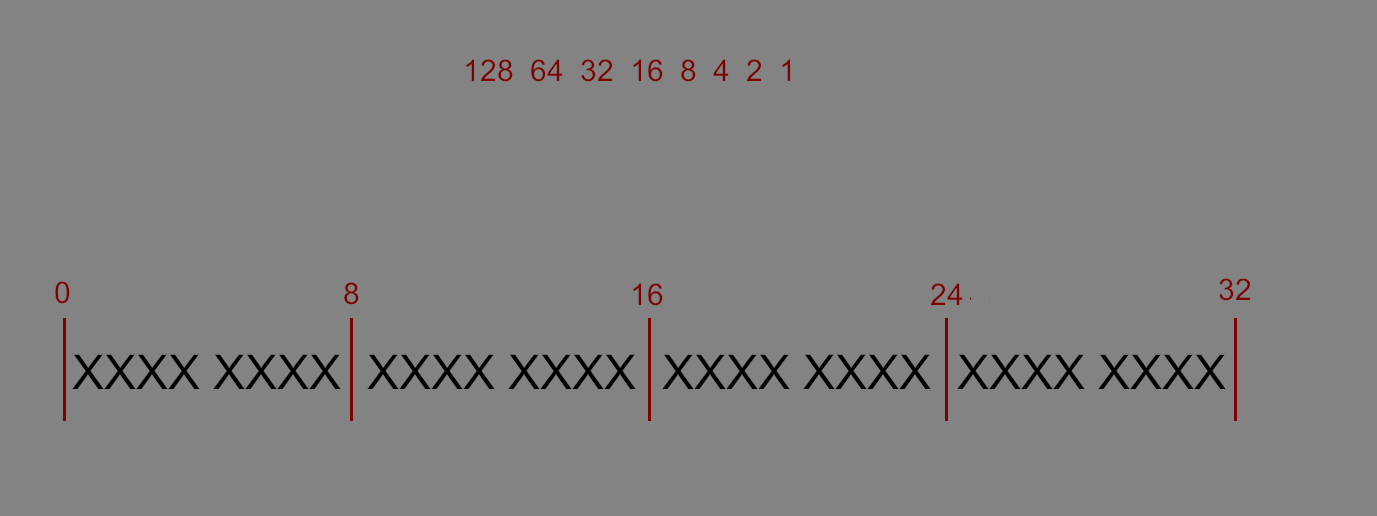
\includegraphics[keepaspectratio,alt={image}]{images/14-subnetting-part1/img-003.png}}
\end{figure}

\begin{enumerate}
\def\labelenumi{\arabic{enumi}.}
\tightlist
\item
  Find the ``magic octet'' where a given IP /Prefix lies, from the bit
  chart shown (boundary digits are inclusive of the octet preceding
  them)
\item
  Count the number of network bits (left to right) in that octet and
  count the same amount, using the red bit slot chart. This'll be your
  address group size.
\item
  Subtract that number from 256 to find your Subnet Mask number used in
  the ``magic octet'' (any octet LEFT of that ``magic octet'' will be
  255, everything RIGHT of that octet will be 0)
\item
  Divide whatever IP octet number is in the ``magic octet'' by the
  address group size.
\end{enumerate}

\begin{itemize}
\tightlist
\item
  If there is a remainder, multiple the whole integer by the address
  group size - your Base Network Address is that value, with every octet
  to the right of that as all 0's
\item
  If there is NO remainder, the IP number in the ``magic octet'' IS the
  Base Network Address is that value, with every octet to the right of
  that as all 0's
\end{itemize}

\begin{enumerate}
\def\labelenumi{\arabic{enumi}.}
\setcounter{enumi}{4}
\tightlist
\item
  The Base Broadcast Number will be Network Base Number + Group Size - 1
  in the ``magic octet'', every value to the right of that octet will be
  255.
\item
  Number of subnets is (2 to the power of the number of network bits in
  the ``magic octet''. ** 2\^{}8 or 256 is equal to 0 **)
\item
  Total Useable Hosts size is (2 to the power of (32 - Prefix Length)
  -2) Example 1:
\end{enumerate}

\begin{lstlisting}
154 . 219 . 154 . 180 /20

Third Octet = Magic

Address Group Size = 16 (L/R count of 4)
256 - 16 = 240 therefore Subnet Mask is 255.255.240.0

Divide 3rd digit / Address Group Size (16)
154 / 16 = 9 (with remainder)
9 * 16 = 144 (Base Network #)

Network : 154 . 219 . 144 . 0

Broadcast Base # = 144 + 16 - 1 = 159

Broadcast : 154. 219 . 159 . 255

Subnets = 2^4 network bits = 16
Total Host Size = (2^(32 - 20))-2 = 4094
\end{lstlisting}

Example 2:

\begin{lstlisting}
84 . 75 . 21 .6 /10

Second Octet = Magic

Address Group Size = 64
256 - 64 = 192

Subnet = 255.192.0.0

75 / 64 = 1 + remainder
1 * 64 = 64 (Base Network #)

Network : 84.64.0.0

Broadcast Base # = 64 + 64 -1 = 127

Broacast : 84.127.255.255

Subnets : 2^2 = 4 Subnets
Total Host Size = (2^(32-10))-2 = 4194302
\end{lstlisting}

\chapter{Subnetting: Part 2}\label{subnetting-part-2}

\section{Class C Networks}\label{class-c-networks}

\begin{figure}
\centering
\pandocbounded{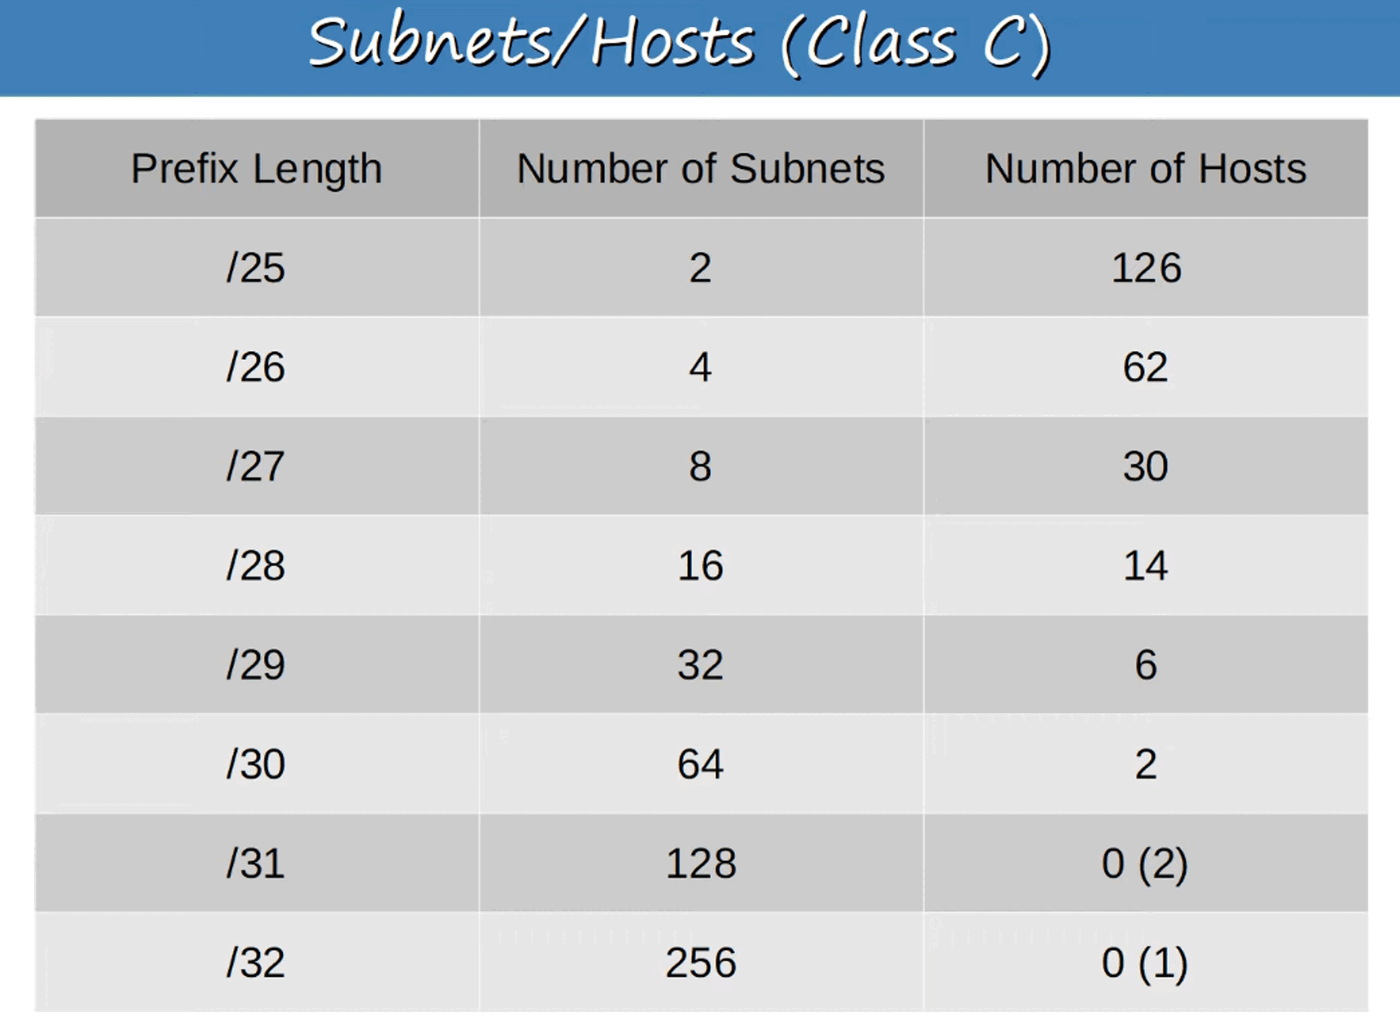
\includegraphics[keepaspectratio,alt={image}]{images/15-subnetting-part2/img-001.png}}
\end{figure}

\section{Class B Networks}\label{class-b-networks}

\begin{figure}
\centering
\pandocbounded{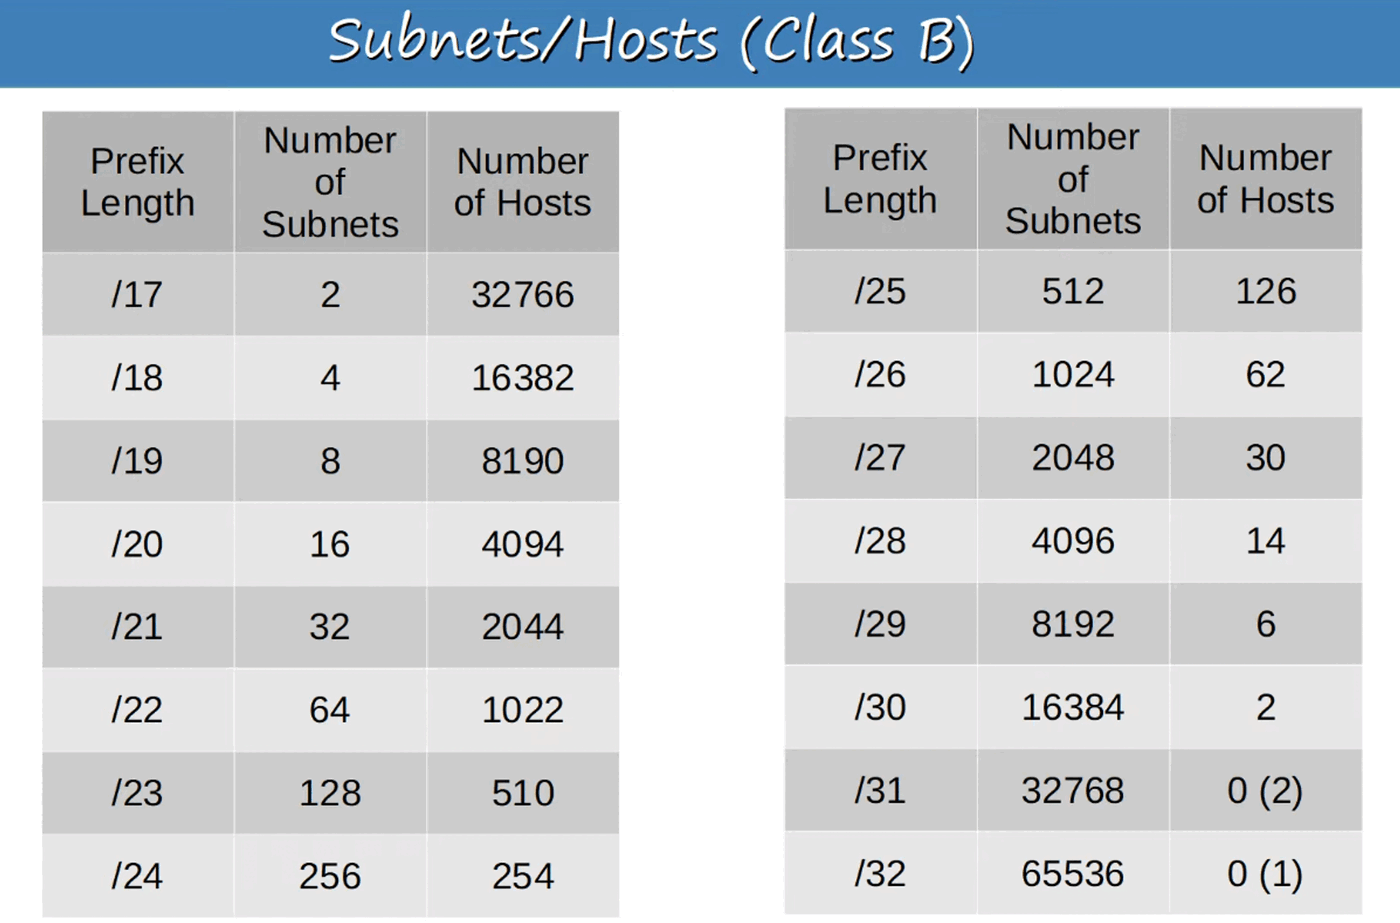
\includegraphics[keepaspectratio,alt={image}]{images/15-subnetting-part2/img-002.png}}
\end{figure}

\chapter{Subnetting with VLSM: Part
3}\label{subnetting-with-vlsm-part-3}

The process of subnetting Class A, Class B, and Class C is identical.

\section{Subnetting Class A Networks}\label{subnetting-class-a-networks}

Given a 10.0.0.0/8 network, you must create 2000 subnets which will
distributed to various enterprises. What prefix length must you use?

2\^{}10 = 1024 so 2\^{}11 = 2048. We have to ``borrow'' 11 bits (Left to
Right) to get enough subnets

0000 1010 . 0000 0000 . 000 \textbar{} 00000 . 0000 0000

8 bits + 8 bits + 3 = 19 bits

0000 1010 . 0000 0000 . 000 \textbar{} 00000 . 0000 0000 1111 1111 .
1111 1111 . 111 \textbar{} 00000 . 0000 0000

255.255.224.0 is the Subnet mask

The answer is /19 (/8 + /11 = /19)

How many hosts per subnet? There are 13 host bits remaining so:

2\^{}13 - 2 = 8190 hosts per subnet

\section{Variable-Length Subnet Masks
(VLSM)}\label{variable-length-subnet-masks-vlsm}

\begin{itemize}
\tightlist
\item
  Until now, we have practiced subnetting using FLSM (Fixed-Length
  Subnet Masks).
\item
  This means that all of the subnets use the same prefix length (ie:
  Subnetting a Class C network into 4 subnets using /26)
\item
  VLSM (Variable-Length Subnet Masks) is the process of creating subnets
  of different sizes, to make your use of network addresses more
  efficient.
\item
  VLSM is more complicated than FLSM, BUT it's easy if you follow the
  steps correctly.
\end{itemize}

\begin{figure}
\centering
\pandocbounded{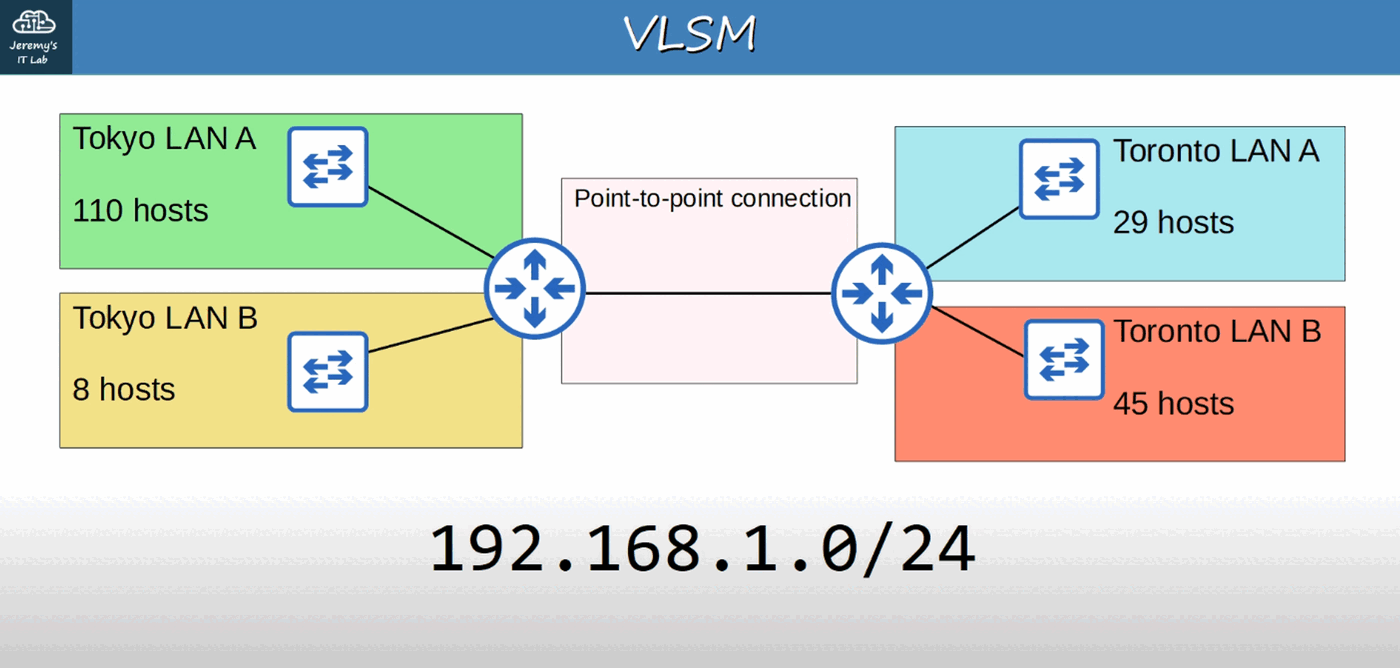
\includegraphics[keepaspectratio,alt={image}]{images/16-subnetting-vlsm-part3/img-001.png}}
\end{figure}

\begin{figure}
\centering
\pandocbounded{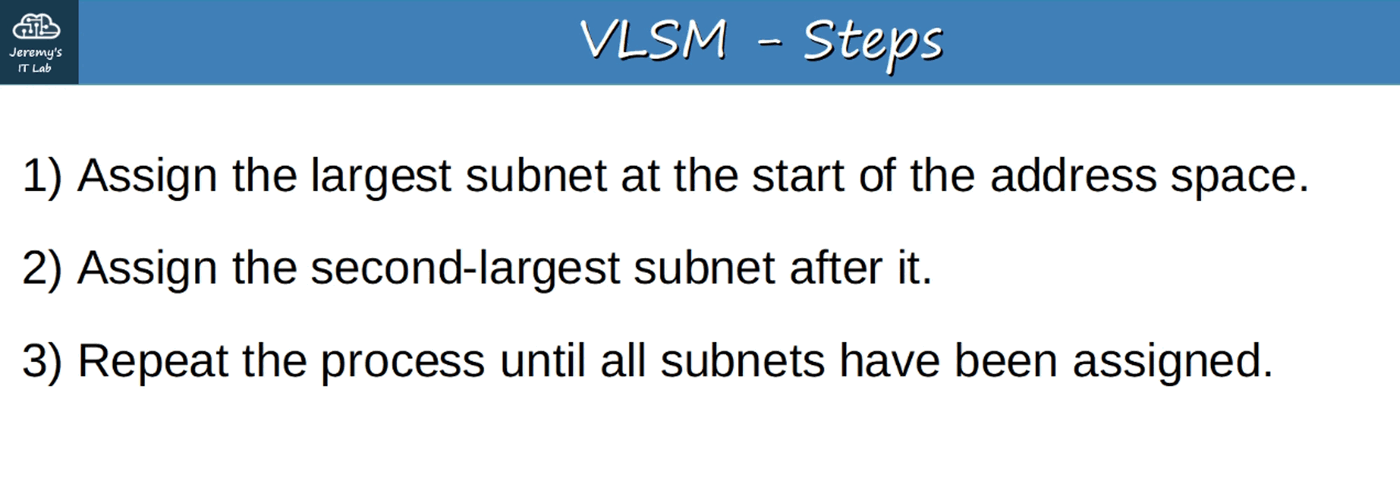
\includegraphics[keepaspectratio,alt={image}]{images/16-subnetting-vlsm-part3/img-002.png}}
\end{figure}

\begin{figure}
\centering
\pandocbounded{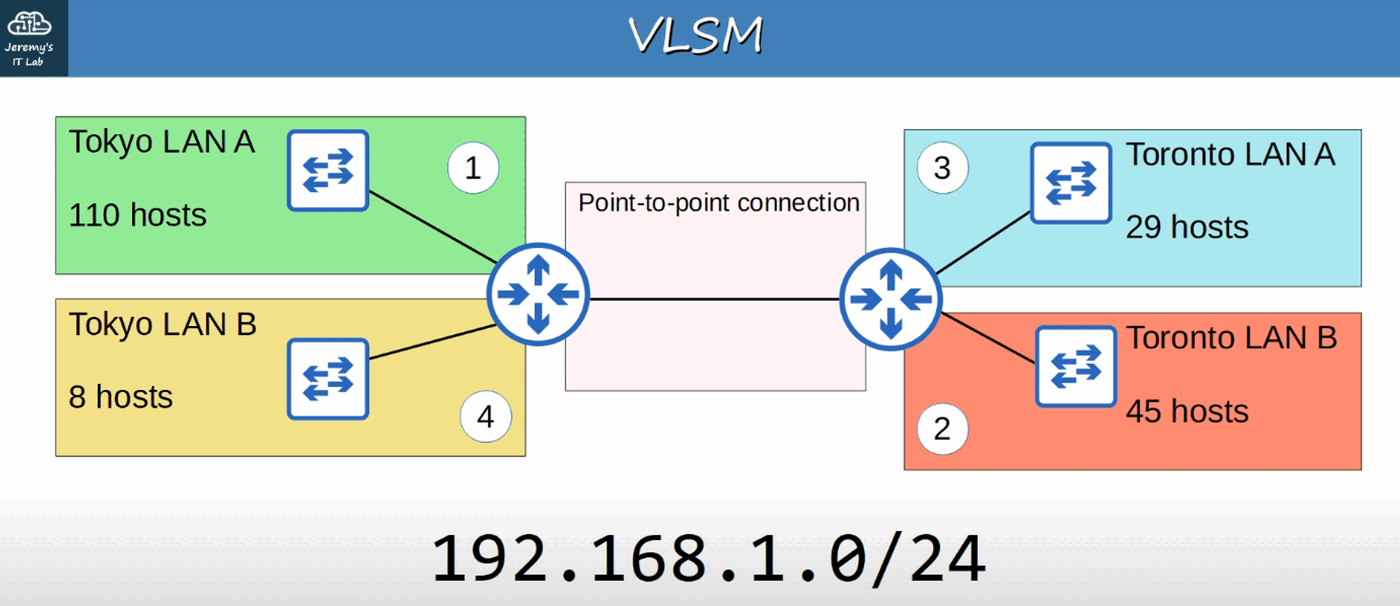
\includegraphics[keepaspectratio,alt={image}]{images/16-subnetting-vlsm-part3/img-003.png}}
\end{figure}

So, in order:

\begin{lstlisting}
TOKYO LAN A (110 HOSTS)
TORONTO LAN B (45 HOSTS)
TORONTO LAN A (29 HOSTS)
TOKYO LAN B (8 HOSTS)
and
THE POINT TO POINT CONNECTION (between the two ROUTERS)
\end{lstlisting}

192.168.1.0 / 24

1000 0000 . 1010 1000 . 0000 0001 \textbar{} 0000 0000 (last is host
octet = 254 usable hosts)

Shifting LEFT - we DOUBLE the \# of hosts Shifting RIGHT - we HALF the
\# of hosts

TOKYO LAN A (we need to borrow 1 host bits, to the RIGHT, to leave
enough for 2\^{}7 or 128 hosts. More than enough for TOKYO A)

so:

\begin{lstlisting}
192.168.1.0/25 (Network Address)
1000 0000 . 1010 1000 . 0000 0001 . 0 | 000 0000

Converting remaining Host Bits to 1s:
0111 1111, we get 127 so

192.168.1.127/25 is the Broadcast Address
\end{lstlisting}

TOKYO LAN A

\begin{lstlisting}
NETWORK ADDRESS: 192.168.1.0/25
BROADCAST ADDRESS: 192.168.1.127/25
FIRST USABLE: 192.168.1.1/25
LAST USABLE: 192.168.1.126/25
TOTAL NUMBER OF USABLE HOSTS: 126 (2^7 -2)

Since TOKYO LAN A is 192.168.1.127, the next Subnet (TOKYO LAN B) starts at 192.168.1.128 (Network Address)
\end{lstlisting}

TORONTO LAN B

\begin{lstlisting}
NETWORK ADDRESS: 192.168.1.128 / 26
BROADCAST ADDRESS: 192.168.1.191 / 26
FIRST USABLE: 192.168.1.129 /26
LAST USABLE: 192.168.1.190 / 26
TOTAL NUMBER OF USABLE HOSTS: 62 (2^6 -2)
\end{lstlisting}

We need to borrow to get enough for 45 hosts.

{\def\LTcaptype{none} % do not increment counter
\begin{longtable}[]{@{}llllllll@{}}
\toprule\noalign{}
128 & 64 & 32 & 16 & 8 & 4 & 2 & 1 \\
\midrule\noalign{}
\endhead
\bottomrule\noalign{}
\endlastfoot
x & x & 0 & 0 & 0 & 0 & 0 & 0 \\
\end{longtable}
}

\begin{lstlisting}
1000 0000 . 1010 1000 . 0000 0001 . 10 | 00 0000

192 . 168 . 1 . 128

1000 0000 . 1010 1000 . 0000 0001 . 10 | 11 1111

192 . 168 . 1 . 191 (Broadcast Address)
\end{lstlisting}

\section{Toronto LAN A}\label{toronto-lan-a}

We need to borrow to get enough for 29 hosts.

{\def\LTcaptype{none} % do not increment counter
\begin{longtable}[]{@{}llllllll@{}}
\toprule\noalign{}
128 & 64 & 32 & 16 & 8 & 4 & 2 & 1 \\
\midrule\noalign{}
\endhead
\bottomrule\noalign{}
\endlastfoot
x & x & x & 0 & 0 & 0 & 0 & 0 \\
\end{longtable}
}

\begin{lstlisting}
1000 0000 . 1010 1000 . 0000 0001 . 110 | 0 0000

192.168.1.192 (Net Address)

1000 0000 . 1010 1000 . 0000 0001 . 110 | 1 1111

192.168.1.224 (Broadcast address)

NETWORK ADDRESS: 192.168.1.192 / 27
BROADCAST ADDRESS: 192.168.1.223 / 27
FIRST USABLE: 192.168.1.193 /27
LAST USABLE: 192.168.1.222 / 27
TOTAL NUMBER OF USABLE HOSTS: 30 hosts (2^5 - 2)
\end{lstlisting}

TOKYO LAN B We need to borrow to get enough for 8 hosts. Remember total
usable hosts is equal to x - 2.

{\def\LTcaptype{none} % do not increment counter
\begin{longtable}[]{@{}llllllll@{}}
\toprule\noalign{}
128 & 64 & 32 & 16 & 8 & 4 & 2 & 1 \\
\midrule\noalign{}
\endhead
\bottomrule\noalign{}
\endlastfoot
x & x & x & x & 0 & 0 & 0 & 0 \\
\end{longtable}
}

\begin{lstlisting}
1000 0000 . 1010 1000 . 0000 0001 . 1110 | 0000

192.168.1.224 (Net Address)

1000 0000 . 1010 1000 . 0000 0001 . 1110 | 1111

192.168.1.239 (Broadcast address)

NETWORK ADDRESS: 192.168.1.224 / 28
BROADCAST ADDRESS: 192.168.1.239 / 28
FIRST USABLE: 192.168.1.225 /28
LAST USABLE: 192.168.1.238 / 28
TOTAL NUMBER OF USABLE HOSTS: 14 hosts (2^4 - 2)
\end{lstlisting}

\section{Point to Point Connections}\label{point-to-point-connections}

We need to borrow to get enough for 4 hosts. Remember total usable hosts
is equal to x - 2.
\textbar128\textbar64\textbar32\textbar16\textbar8\textbar4\textbar2\textbar1\textbar{}
\textbar---\textbar--\textbar--\textbar--\textbar-\textbar-\textbar-\textbar-\textbar{}
\textbar x \textbar x \textbar{} x\textbar{}
x\textbar x\textbar x\textbar0\textbar0\textbar{}

\begin{lstlisting}
1000 0000 . 1010 1000 . 0000 0001 . 1111 00 | 00

192.168.1.240 (Net Address)

1000 0000 . 1010 1000 . 0000 0001 . 1111 00 | 11

192.168.1.243 (Broadcast address)

NETWORK ADDRESS: 192.168.1.240 / 30
BROADCAST ADDRESS: 192.168.1.243 / 30
FIRST USABLE: 192.168.1.241 / 30
LAST USABLE: 192.168.1.242 / 30
TOTAL NUMBER OF USABLE HOSTS: 2 hosts (2^2 - 2)
\end{lstlisting}

\section{Additional Practice for
Subnetting}\label{additional-practice-for-subnetting}

\href{http://www.subnettingquestions.com/}{http://www.subnettingquestions.com}
\href{http://subnetting.org/}{http://subnetting.org}
\href{https://subnettingpractice.com/}{https://subnettingpractice.com}
*** Preferred site ***

\chapter{VLANs: Part 1}\label{vlans-part-1}

WHAT IS A LAN ?

\begin{itemize}
\tightlist
\item
  A LAN is a single BROADCAST DOMAIN, including all devices in that
  broadcast domain.
\end{itemize}

\section{Broadcast Domains}\label{broadcast-domains}

\begin{itemize}
\tightlist
\item
  A BROADCAST DOMAIN is the group of devices which will receive a
  BROADCAST FRAME (Destination MAC : FFFF.FFFF.FFFF) sent by any one of
  the members.
\end{itemize}

Image of LAN with FOUR BROADCAST DOMAINS (192.168.1.0 / 24)

\begin{figure}
\centering
\pandocbounded{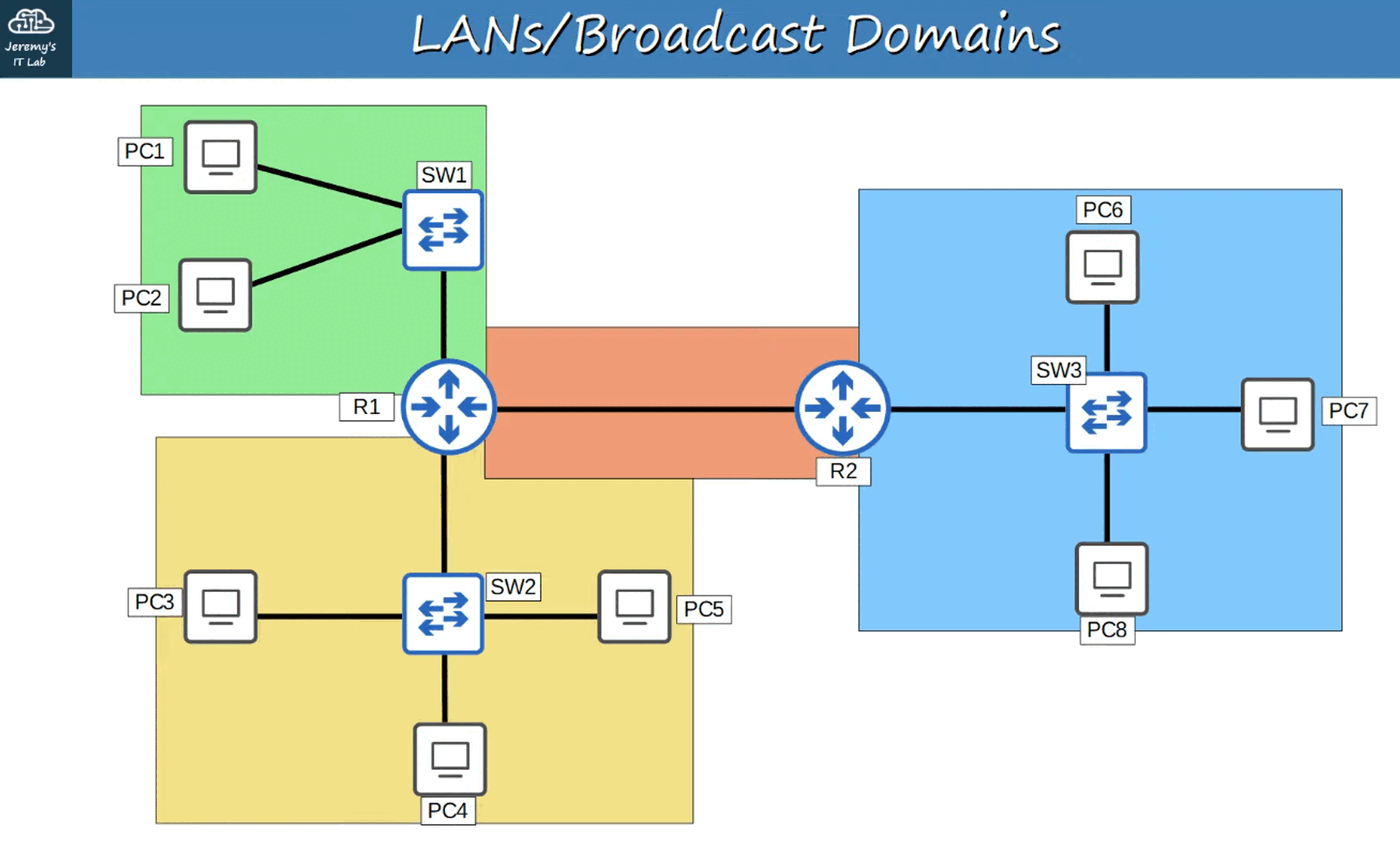
\includegraphics[keepaspectratio,alt={image}]{images/17-vlan-part1/img-001.png}}
\end{figure}

Performance :

Lots of unnecessary BROADCAST traffic can reduce network performance.

\begin{figure}
\centering
\pandocbounded{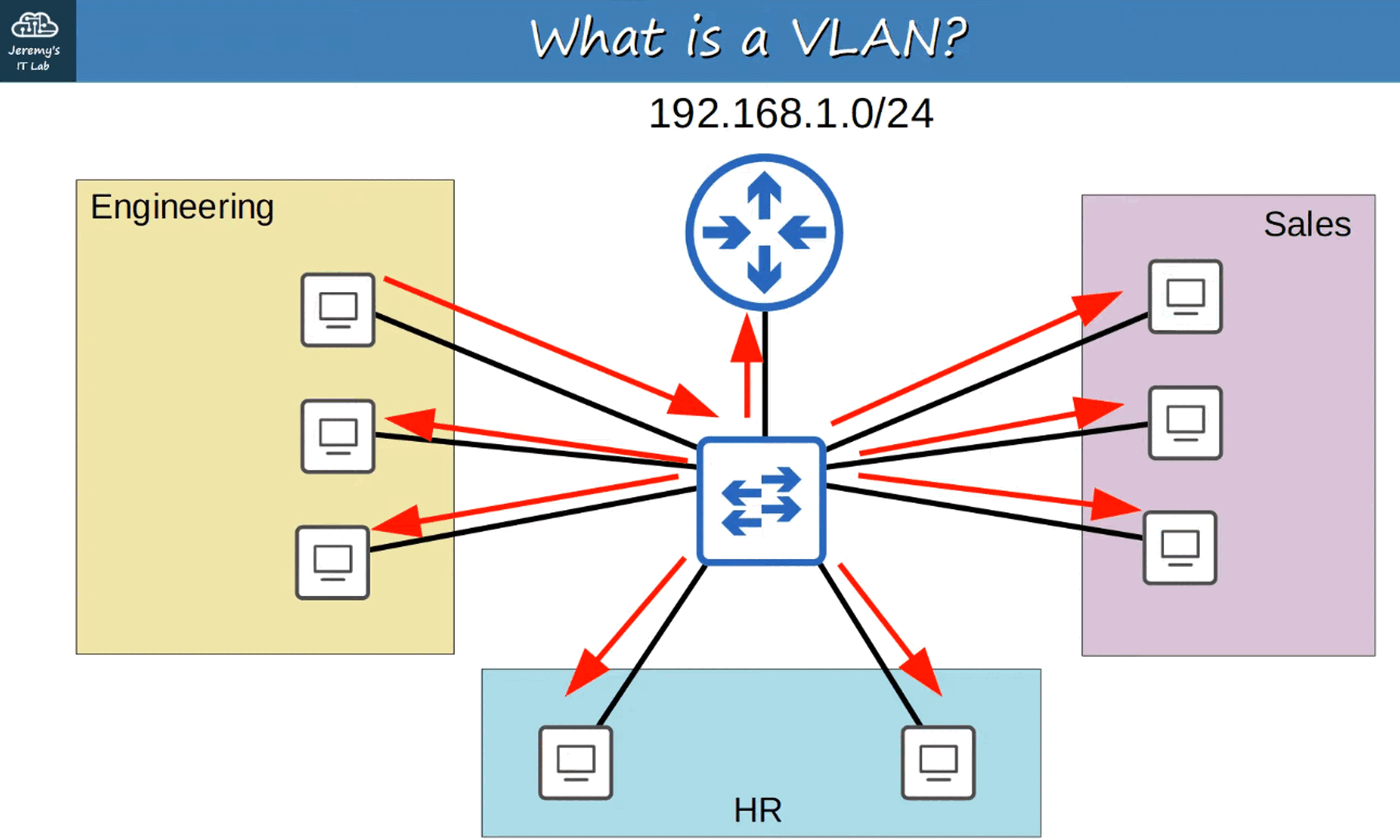
\includegraphics[keepaspectratio,alt={image}]{images/17-vlan-part1/img-002.png}}
\end{figure}

BROADCAST FRAME flooding all our subnets with unnecessary traffic.

\begin{figure}
\centering
\pandocbounded{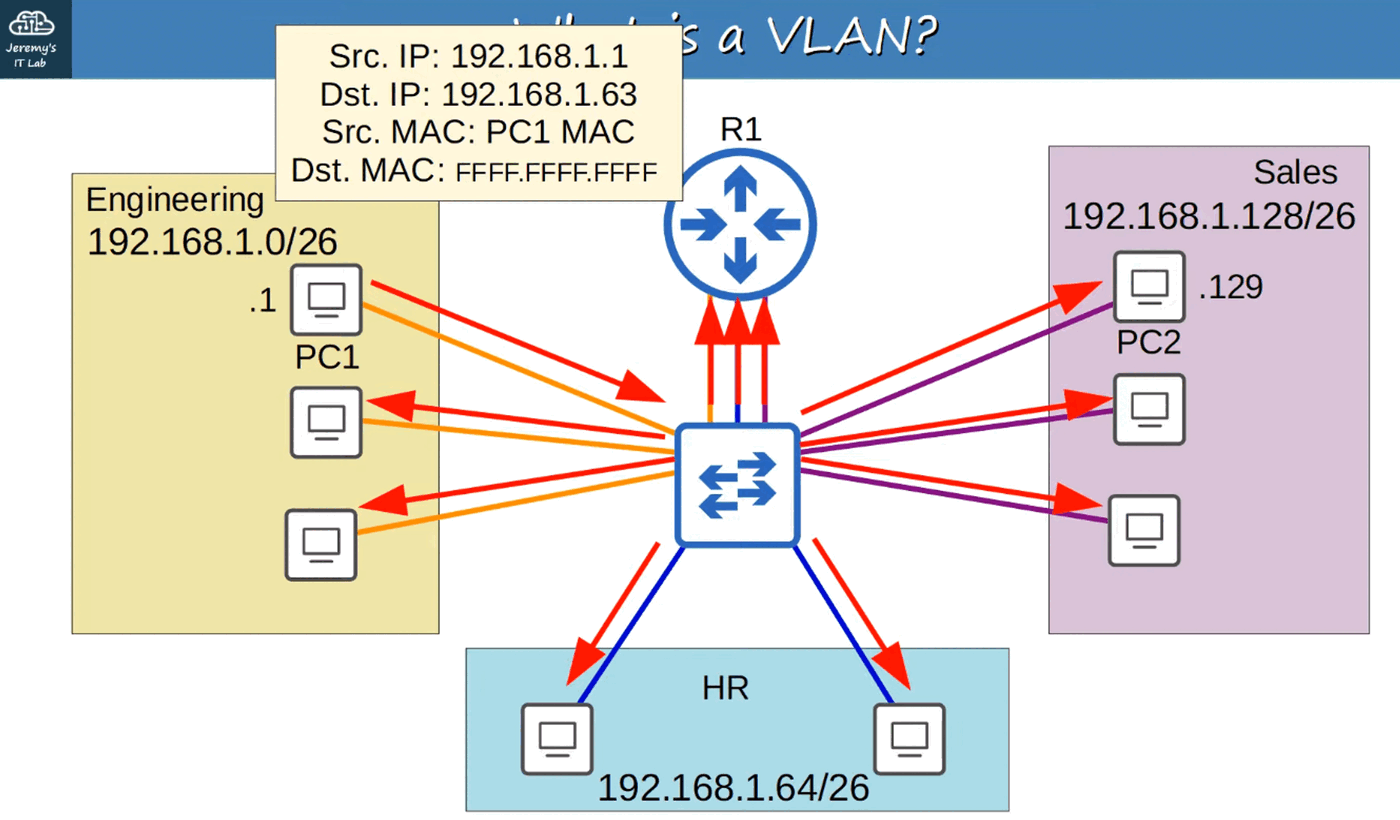
\includegraphics[keepaspectratio,alt={image}]{images/17-vlan-part1/img-003.png}}
\end{figure}

Security :

Even within the same office, you want to limit who has access to what.
You can apply security policies on a ROUTER / FIREWALL. Because this is
one LAN, PC's can reach each other directly, without traffic passing
through the router. So, even if you configure security policies, they
won't have any effect.

\begin{figure}
\centering
\pandocbounded{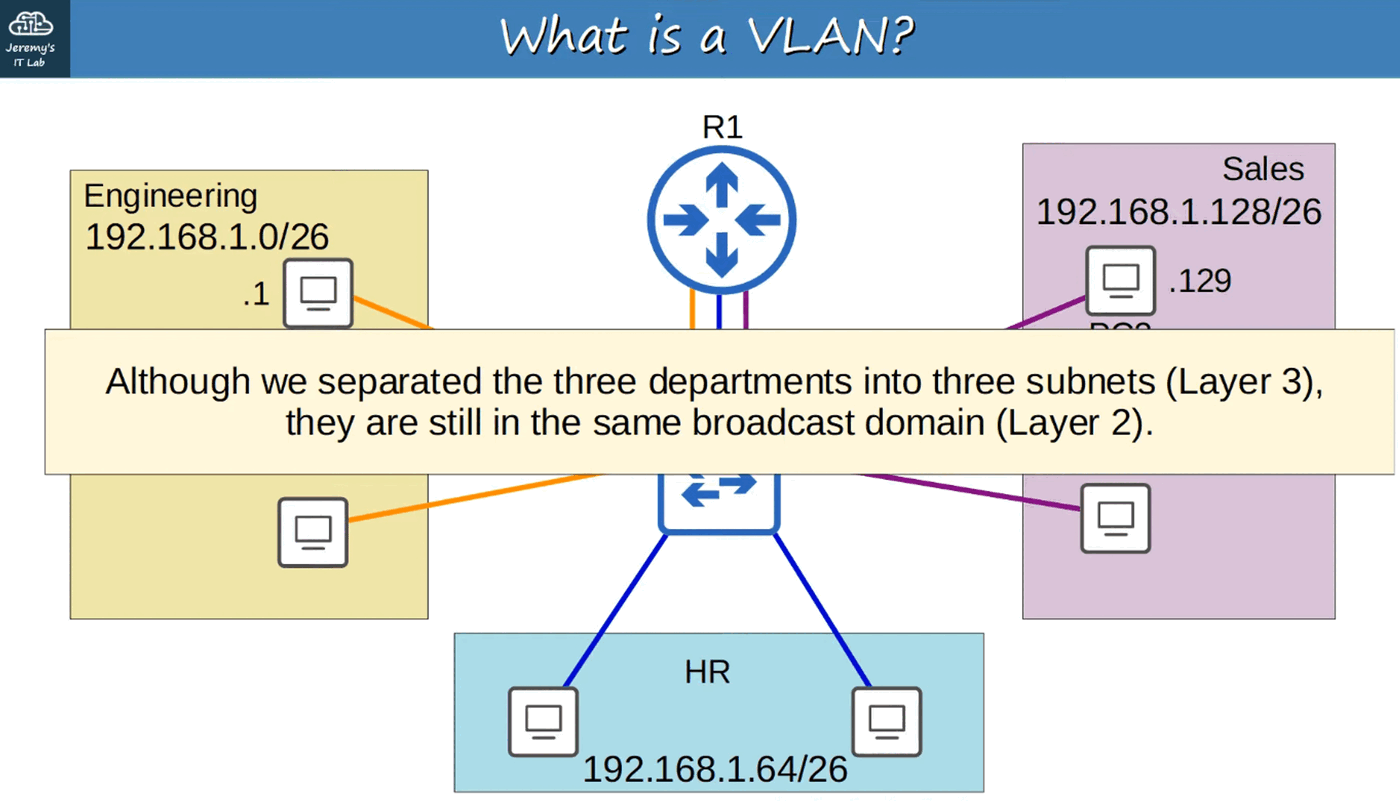
\includegraphics[keepaspectratio,alt={image}]{images/17-vlan-part1/img-004.png}}
\end{figure}

WHAT IS A VLAN ?

\section{VLANs}\label{vlans}

\begin{itemize}
\tightlist
\item
  logically separate end-hosts at LAYER 2
\item
  are configured on Layer 2 SWITCHES on a per-interface basis.
\item
  any END HOST connected to that interface is part of that VLAN
\end{itemize}

PURPOSE OF VLANs:

Network Performance :

\begin{itemize}
\tightlist
\item
  Reduce unnecessary BROADCAST traffic, which helps prevent network
  congestion, and improve network performance
\end{itemize}

Network Security :

\begin{itemize}
\tightlist
\item
  Limiting BROADCAST and unknown UNICAST traffic, also improves network
  security, since messages won't be received by devices outside of the
  VLAN
\end{itemize}

\begin{figure}
\centering
\pandocbounded{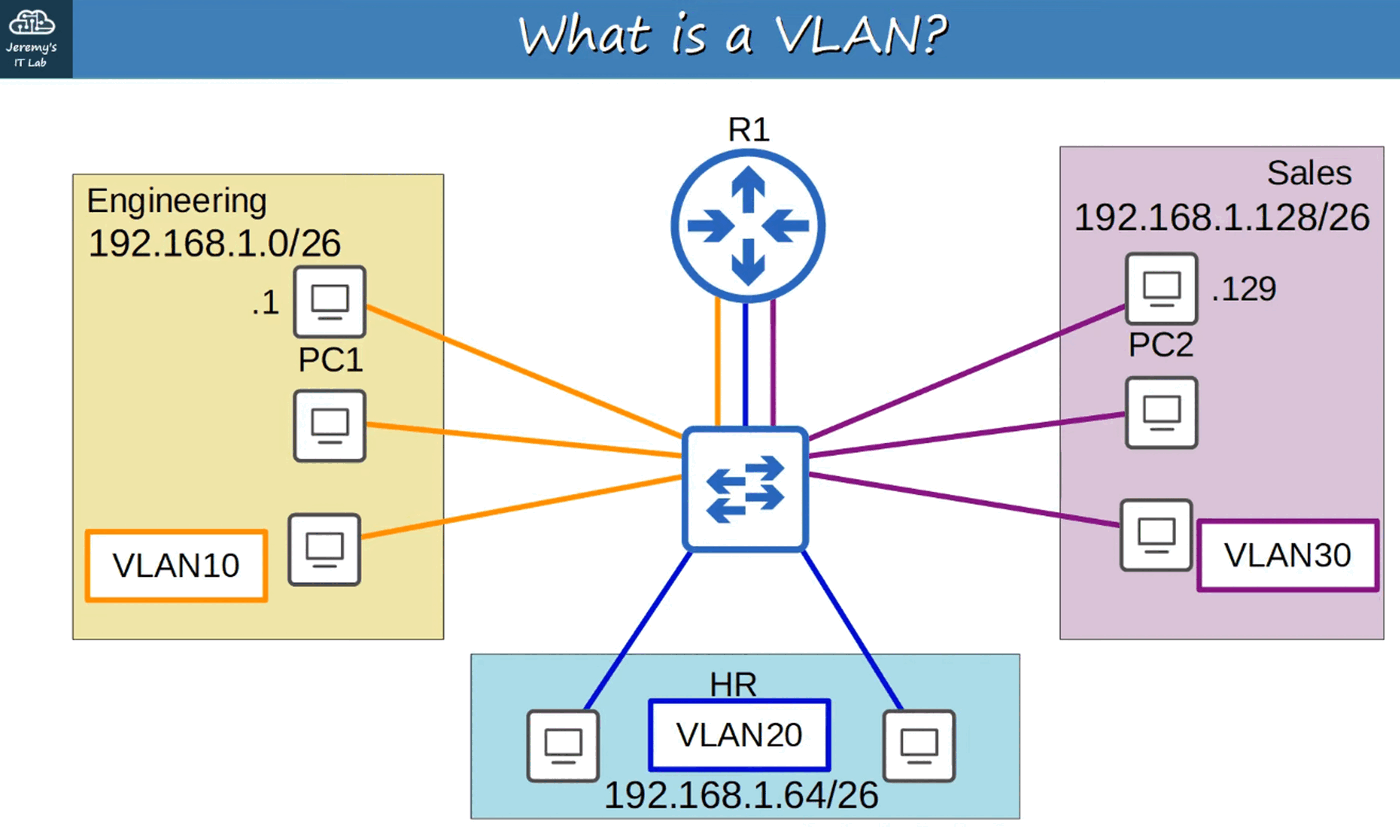
\includegraphics[keepaspectratio,alt={image}]{images/17-vlan-part1/img-005.png}}
\end{figure}

SWITCHES do not forward traffic directly between HOSTS in different
VLANS

\begin{figure}
\centering
\pandocbounded{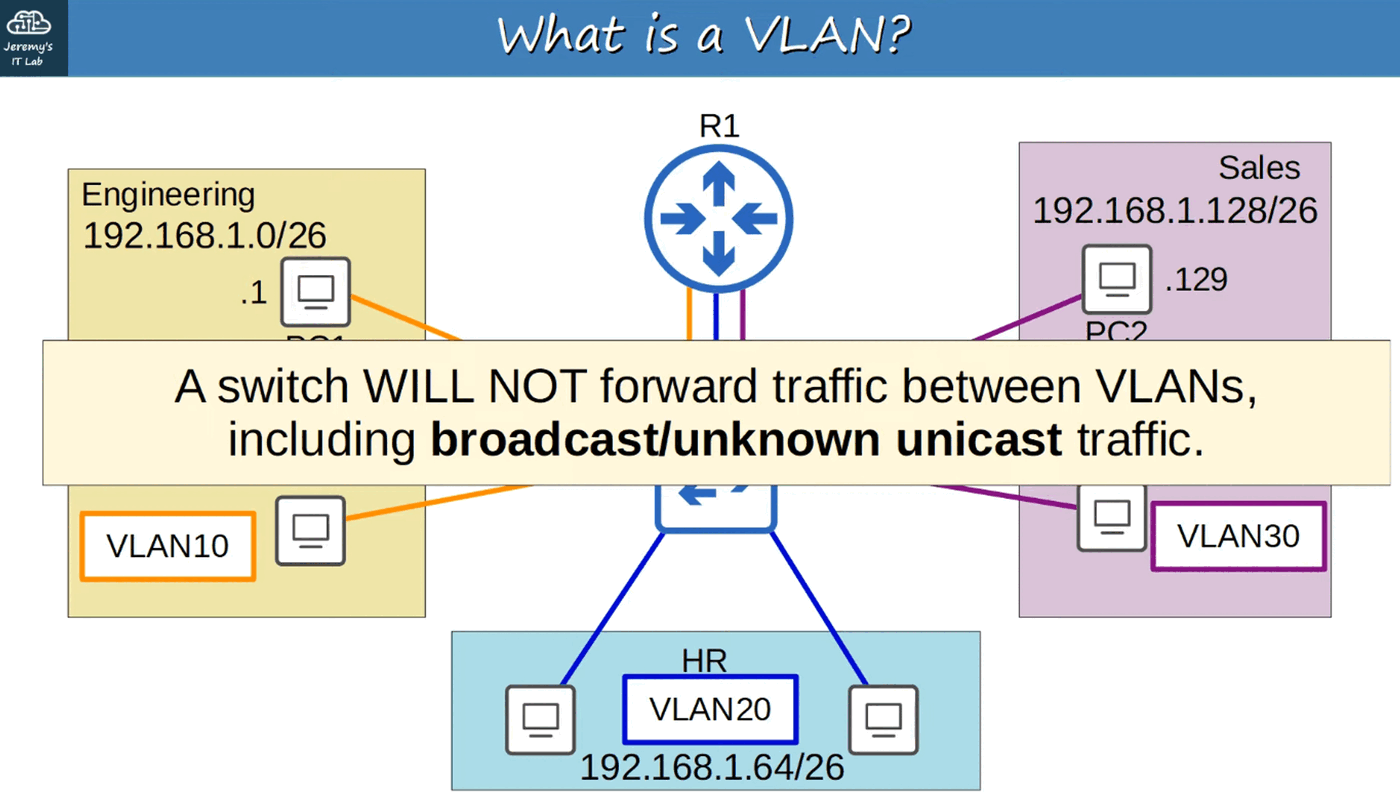
\includegraphics[keepaspectratio,alt={image}]{images/17-vlan-part1/img-006.png}}
\end{figure}

\begin{figure}
\centering
\pandocbounded{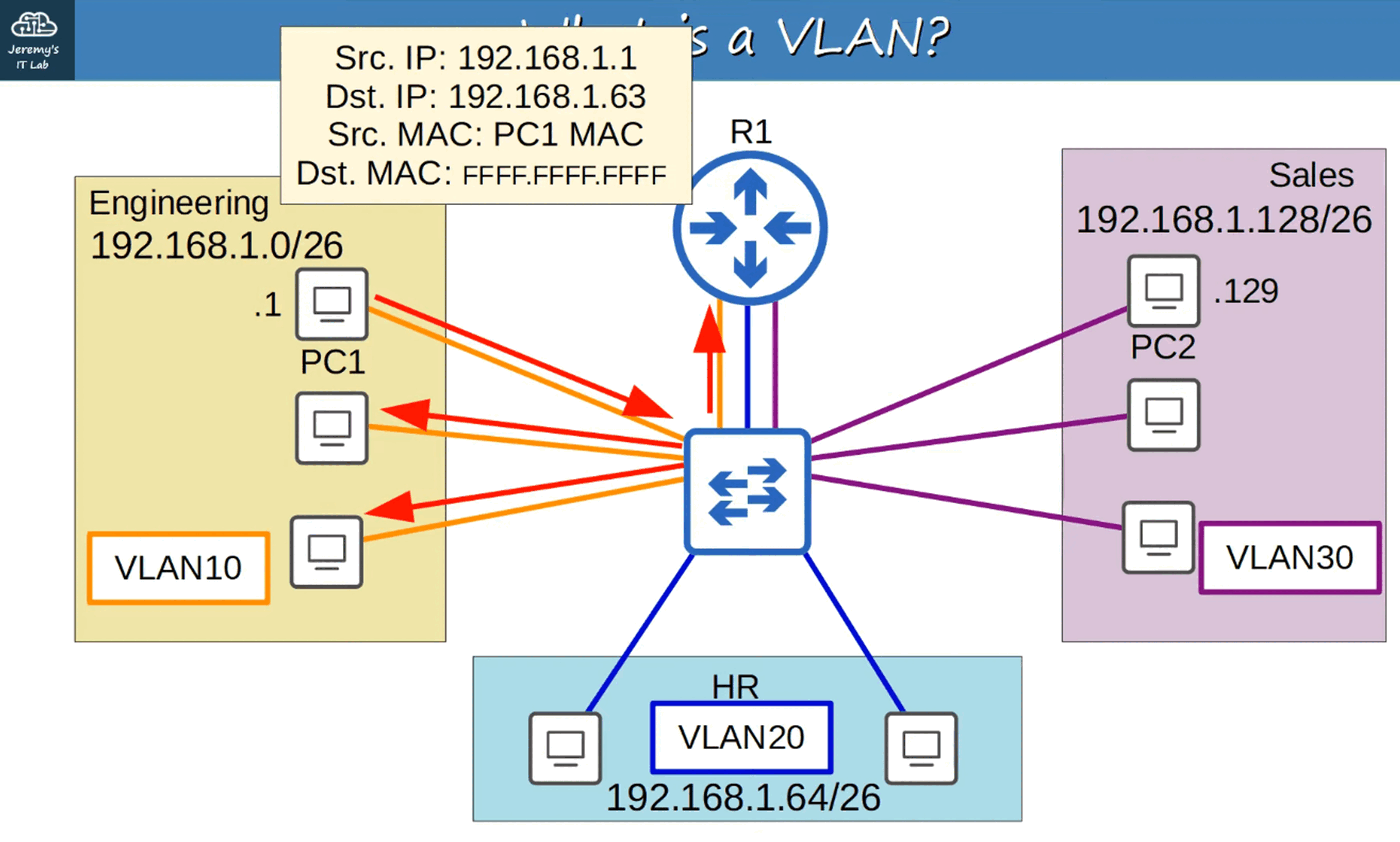
\includegraphics[keepaspectratio,alt={image}]{images/17-vlan-part1/img-007.png}}
\end{figure}

Sending Packets to another VLAN (Routed through R1)

\begin{figure}
\centering
\pandocbounded{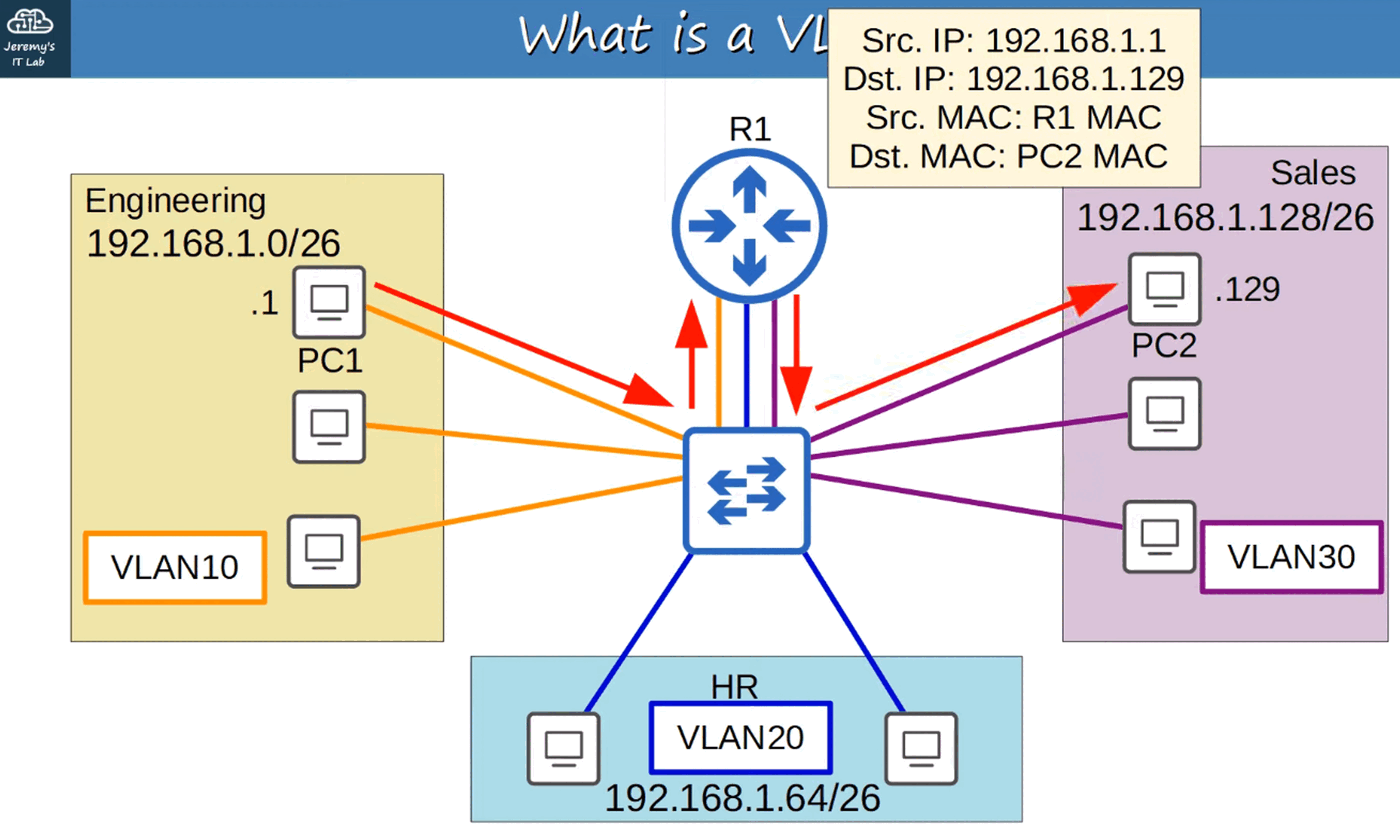
\includegraphics[keepaspectratio,alt={image}]{images/17-vlan-part1/img-008.png}}
\end{figure}

\begin{figure}
\centering
\pandocbounded{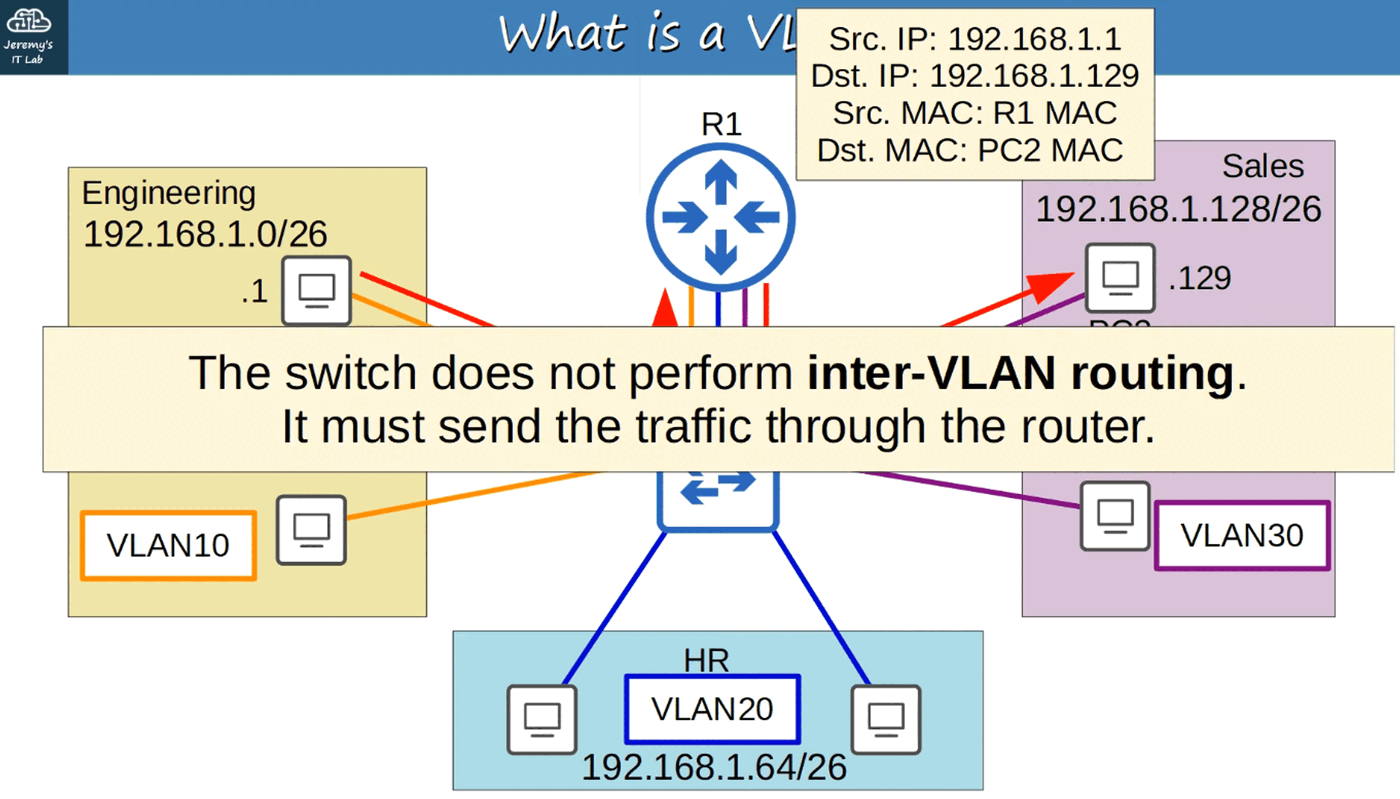
\includegraphics[keepaspectratio,alt={image}]{images/17-vlan-part1/img-009.png}}
\end{figure}

\section{How to Configure VLANs on Cisco
Switches}\label{how-to-configure-vlans-on-cisco-switches}

\#show vlan brief

\begin{figure}
\centering
\pandocbounded{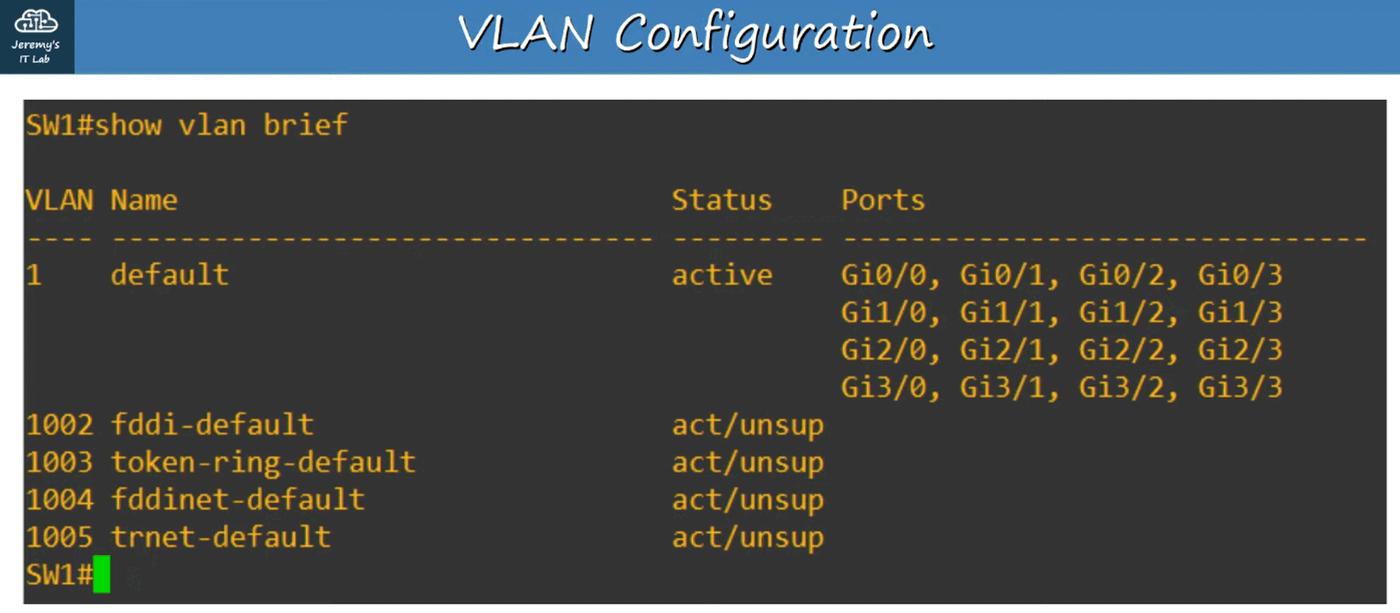
\includegraphics[keepaspectratio,alt={image}]{images/17-vlan-part1/img-010.png}}
\end{figure}

Shows which VLANS that exist on the SWITCH and what INTERFACES are in
each VLAN

VLANs 1 (DEFAULT), 1002-1005 exist by default and \textbf{cannot be
deleted (5 VLANs)}

\section{How to Assign Interfaces to a
VLAN}\label{how-to-assign-interfaces-to-a-vlan}

\begin{figure}
\centering
\pandocbounded{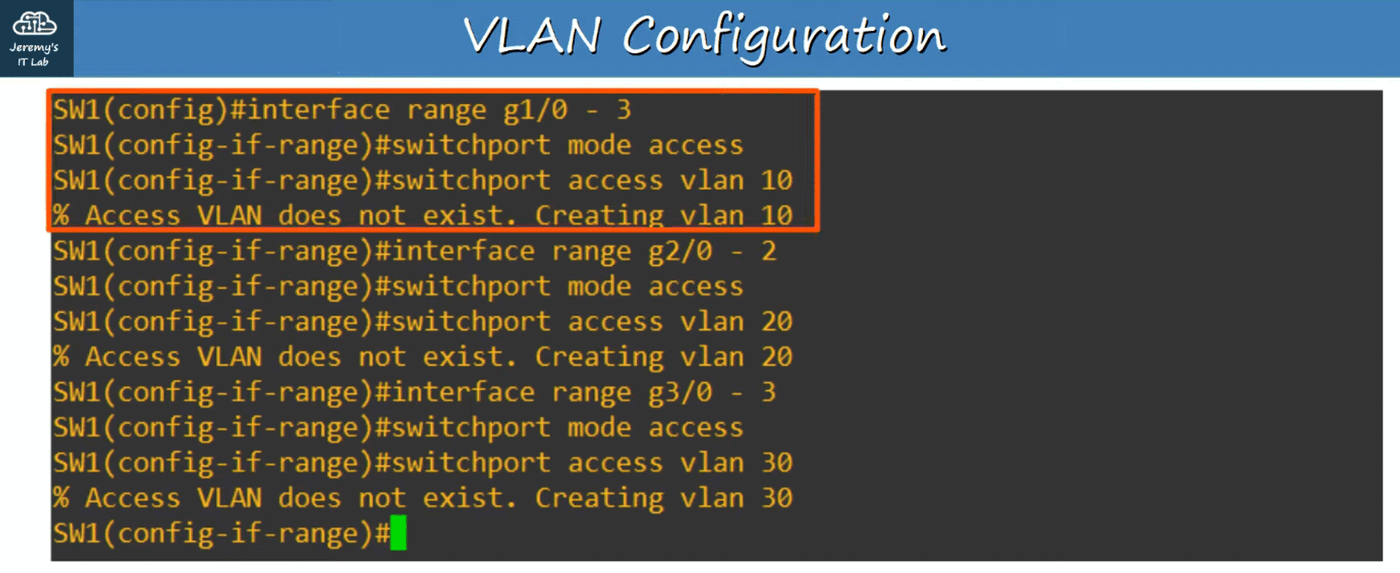
\includegraphics[keepaspectratio,alt={image}]{images/17-vlan-part1/img-011.png}}
\end{figure}

\begin{enumerate}
\def\labelenumi{\arabic{enumi})}
\item
  Use the ``interface range'' command to select all the interfaces at
  once
\item
  Use the ``switchport mode access'' command to set the interface as an
  ACCESS PORT
\end{enumerate}

WHAT IS AN ACCESS PORT?

\begin{itemize}
\tightlist
\item
  An ACCESS PORT is a SWITCHPORT which belongs to a single VLAN, and
  usually connects to end hosts like PCs.
\end{itemize}

SWITCHPORTS which carry multiple VLANs are called ``TRUNK PORTS'' (more
info on TRUNK in next chapter)

\begin{enumerate}
\def\labelenumi{\arabic{enumi})}
\setcounter{enumi}{2}
\tightlist
\item
  Use the ``switchport access'' command to assign a VLAN to a PORT
\end{enumerate}

\begin{figure}
\centering
\pandocbounded{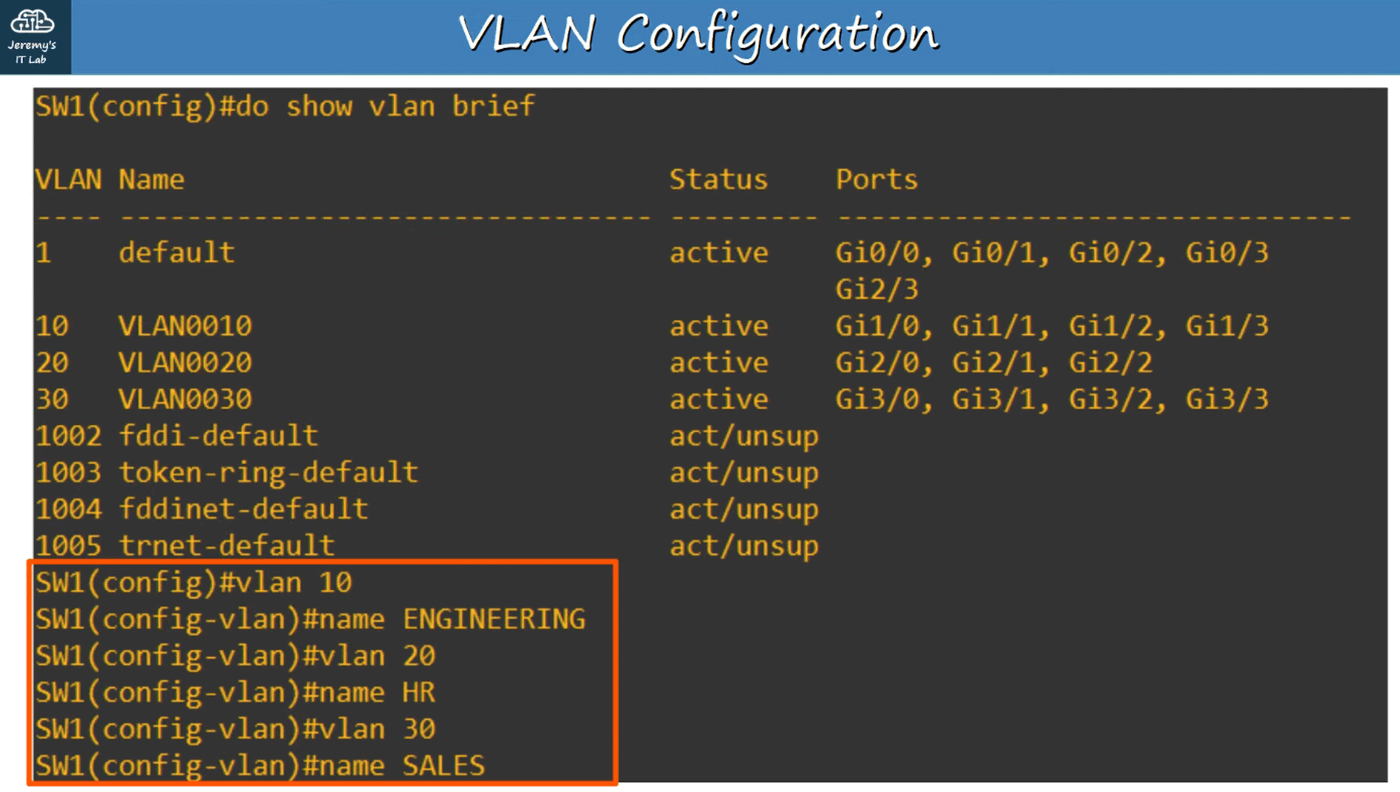
\includegraphics[keepaspectratio,alt={image}]{images/17-vlan-part1/img-012.png}}
\end{figure}

Use ``\#vlan \textless\#\textgreater'' to enter \textbf{Configuration
Mode} for a given VLAN (this can also create a VLAN)

Use ``\#name \textless name\textgreater'' to configure a NAME for your
VLAN

To check your VLAN configuration, use ``\#show vlan brief''

\begin{figure}
\centering
\pandocbounded{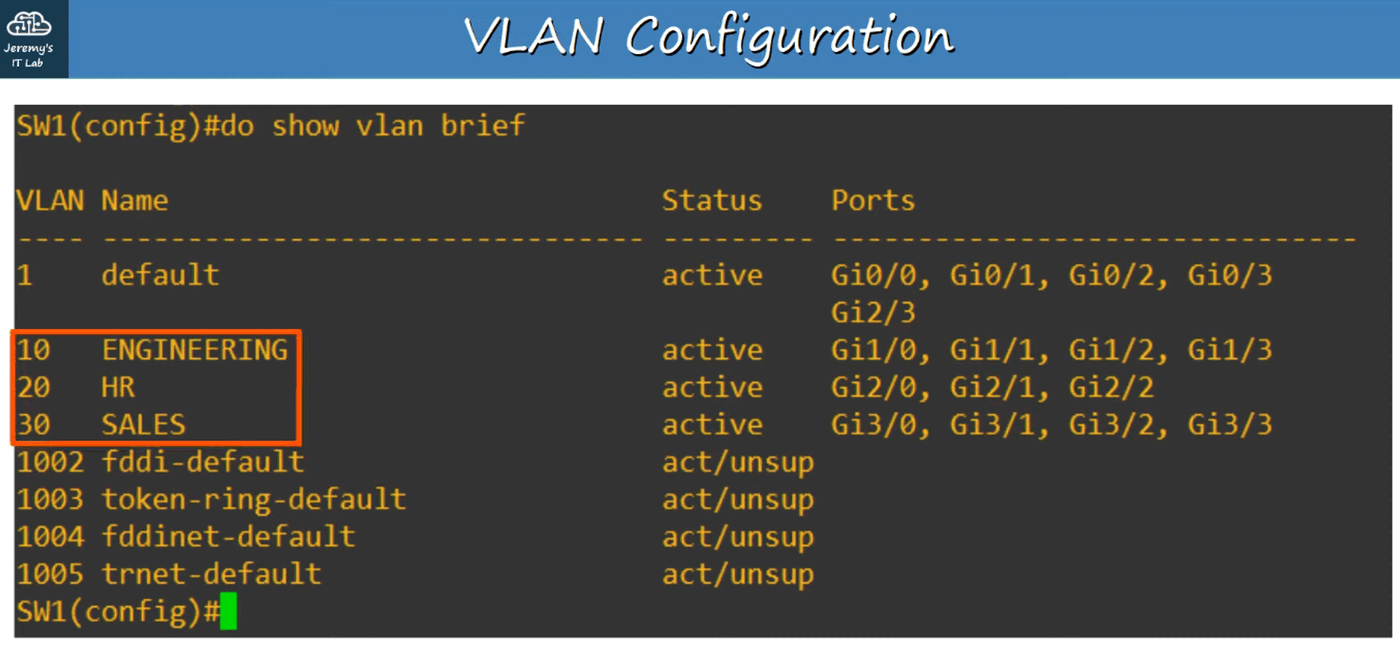
\includegraphics[keepaspectratio,alt={image}]{images/17-vlan-part1/img-013.png}}
\end{figure}

Testing VLAN 10

Pinging from PC1 using 255.255.255.255 (FFFF:FFFF:FFFF) floods broadcast
packets to R1 and VLAN10 hosts only

\begin{figure}
\centering
\pandocbounded{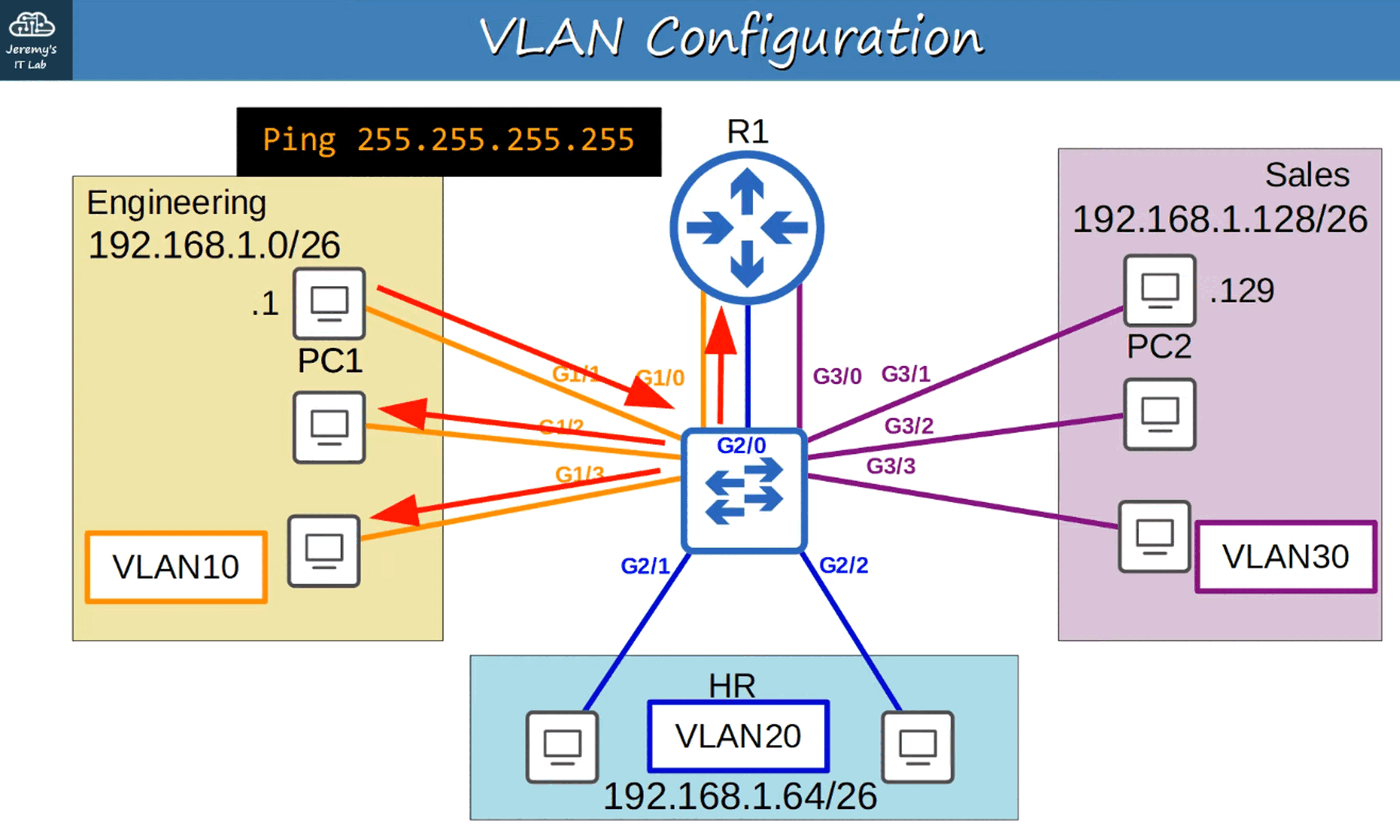
\includegraphics[keepaspectratio,alt={image}]{images/17-vlan-part1/img-014.png}}
\end{figure}

\chapter{VLANs: Part 2}\label{vlans-part-2}

Basic VLAN topology from PART 1

\begin{figure}
\centering
\pandocbounded{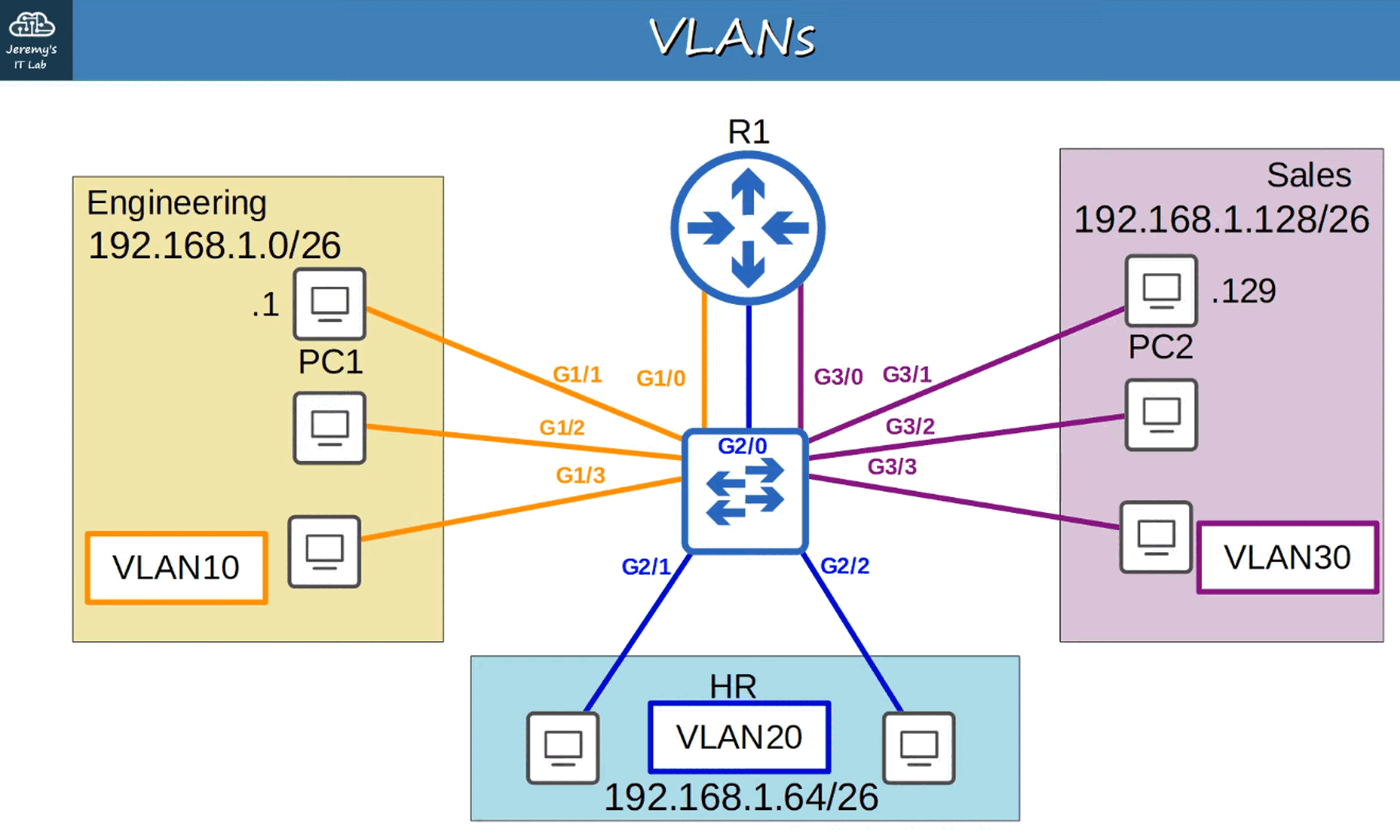
\includegraphics[keepaspectratio,alt={image}]{images/18-vlan-part2/img-001.png}}
\end{figure}

What about THIS Network Topology ?

\begin{figure}
\centering
\pandocbounded{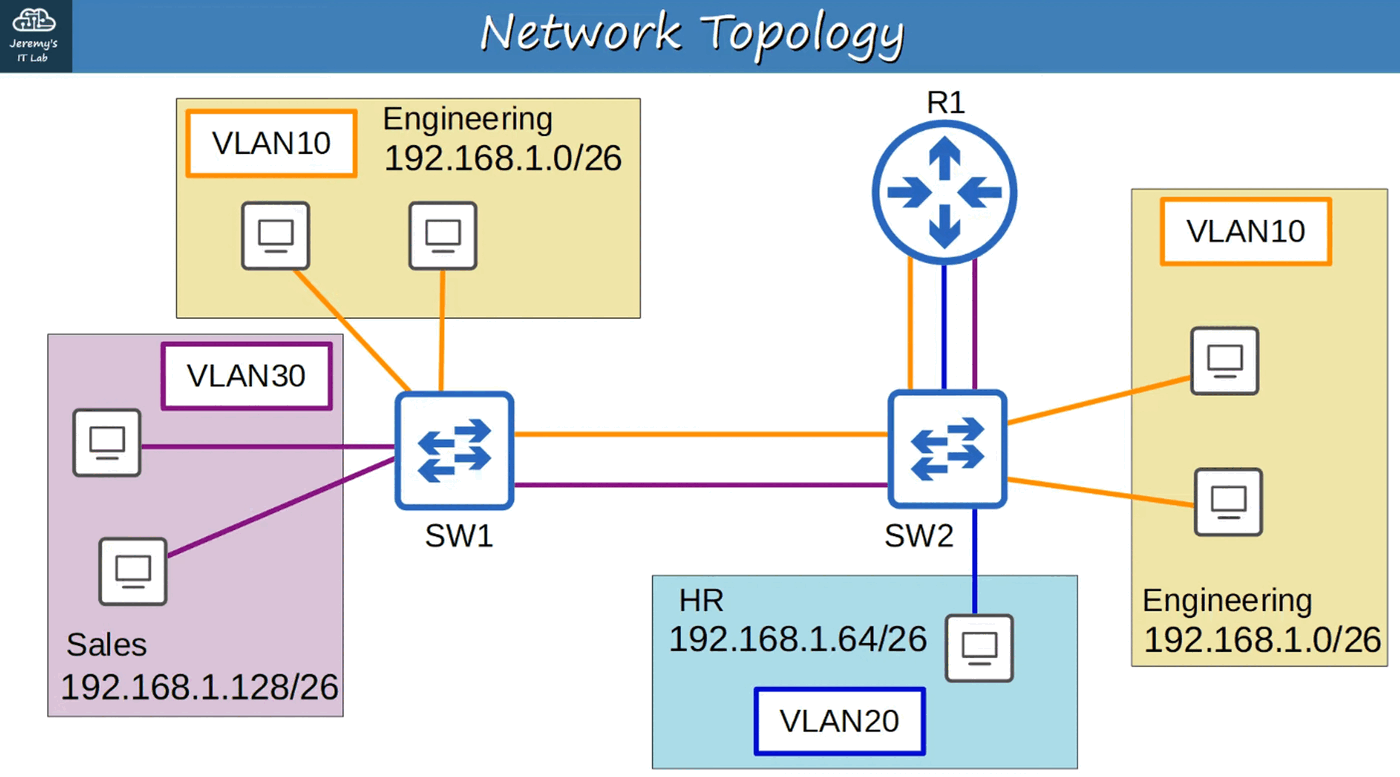
\includegraphics[keepaspectratio,alt={image}]{images/18-vlan-part2/img-002.png}}
\end{figure}

Notice this one has TWO Switches (SW1 and SW2) and ENGINEERING (VLAN 10)
has two separate locations on the network.

\section{Trunk Ports}\label{trunk-ports}

\begin{itemize}
\item
  In a small network with few VLANS, it's possible to use a separate
  interface for EACH VLAN when connecting SWITCHES to SWITCHES, and
  SWITCHES to ROUTERS
\item
  HOWEVER, when the number of VLANS increases, this is not viable. It
  will result in wasted interfaces, and often ROUTERS won't have enough
  INTERFACES for each VLAN
\item
  You can use TRUNK PORTS to carry traffic from multiple VLANS over a
  single interface
\end{itemize}

A TRUNK PORT carrying multiple VLAN connections over single interface

\begin{figure}
\centering
\pandocbounded{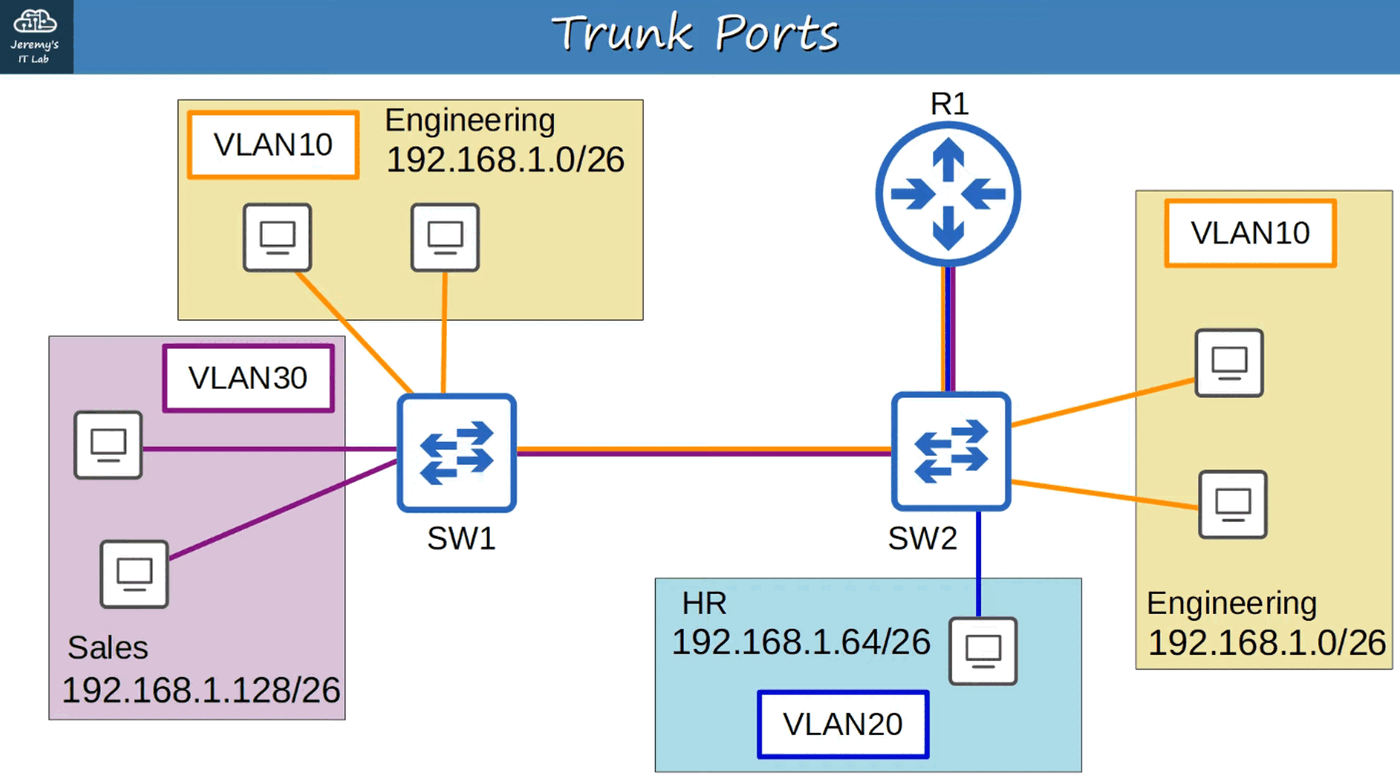
\includegraphics[keepaspectratio,alt={image}]{images/18-vlan-part2/img-003.png}}
\end{figure}

\begin{figure}
\centering
\pandocbounded{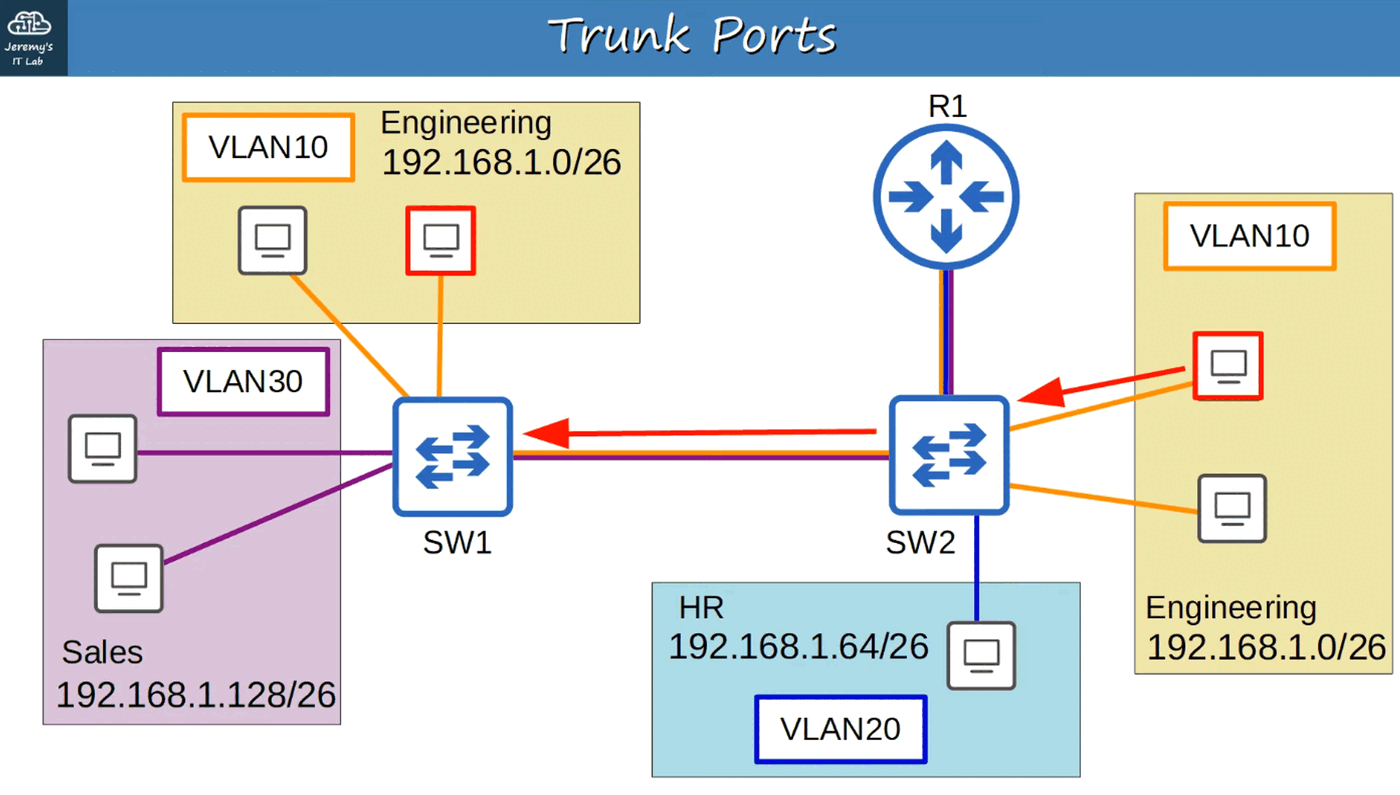
\includegraphics[keepaspectratio,alt={image}]{images/18-vlan-part2/img-004.png}}
\end{figure}

How does a packet know WHICH VLAN to send traffic to over the TRUNK PORT
?

VLAN TAGS !

SWITCHES will ``tag'' all frames that they send over a TRUNK LINK. This
allows the receiving SWITCH to know which VLAN the frame belongs to.

TRUNK PORT = ``Tagged'' ports

ACCESS PORT = ``Untagged'' ports

\section{VLAN Tagging}\label{vlan-tagging}

\begin{itemize}
\tightlist
\item
  There are TWO main TRUNK protocols:

  \begin{itemize}
  \tightlist
  \item
    ISL (Inter-Switch Link)
  \item
    IEEE 802.1Q (also known as ``dot1q'')
  \end{itemize}
\end{itemize}

ISL is an old Cisco proprietary protocol created before industry
standard IEEE 802.1Q

IEEE 802.1Q is an industry standard protocol created by the IEEE
(Institute of Electrical and Electronics Engineers)

You will probably NEVER use ISL in the real world; even modern Cisco
equipment doesn't use it.

For the CCNA, you will only need to learn 802.1Q

ETHERNET HEADER with 802.1Q

\begin{figure}
\centering
\pandocbounded{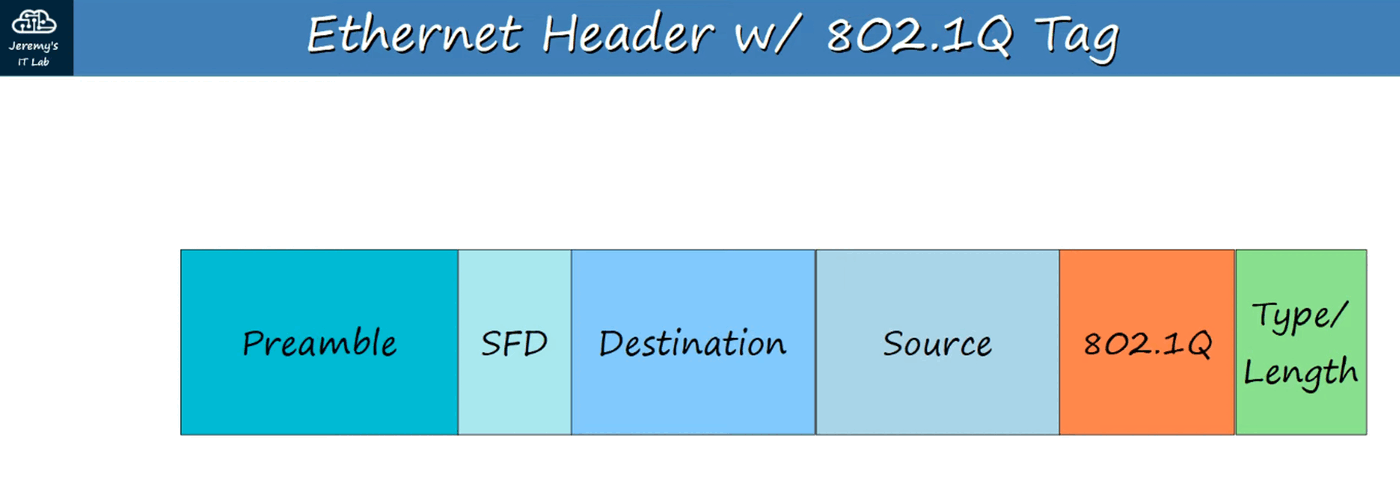
\includegraphics[keepaspectratio,alt={image}]{images/18-vlan-part2/img-005.png}}
\end{figure}

\begin{itemize}
\tightlist
\item
  The 802.1Q TAG Is inserted between the SOURCE and TYPE/LENGTH fields
  in the ETHERNET FRAME
\item
  The TAG is 4 bytes (32 bits) in length
\item
  The TAG consists of TWO main fields:

  \begin{itemize}
  \tightlist
  \item
    Tag Protocol Identifier (TPID)
  \item
    Tag Control Information (TCI)

    \begin{itemize}
    \tightlist
    \item
      TCI consists of THREE sub-fields:
    \end{itemize}
  \end{itemize}
\end{itemize}

\begin{figure}
\centering
\pandocbounded{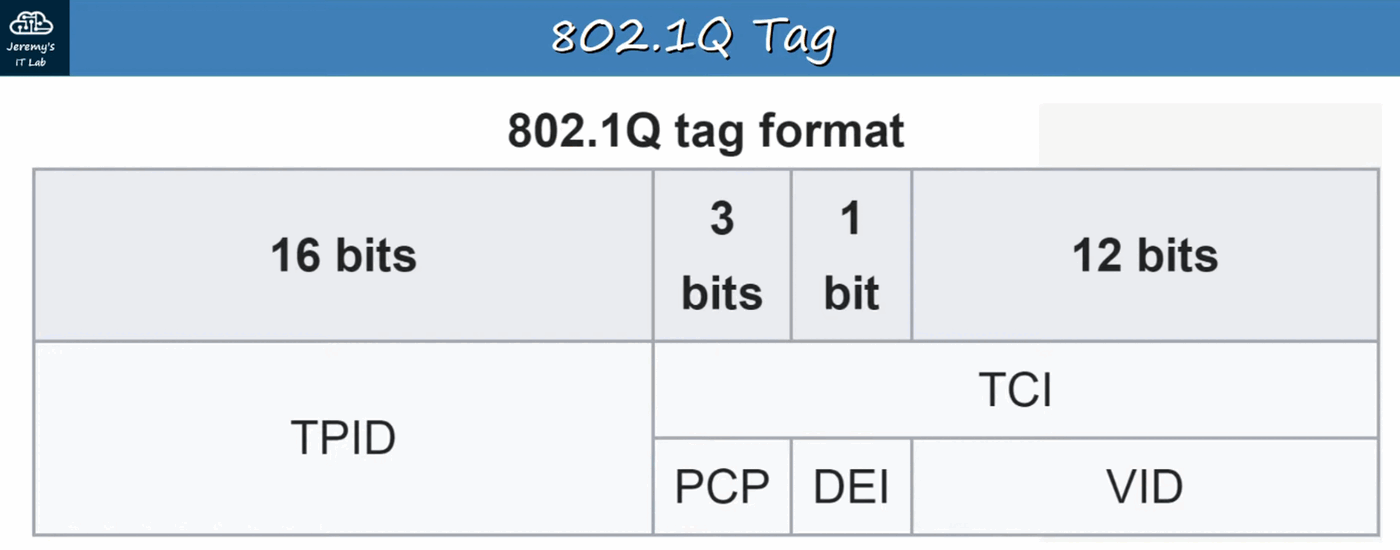
\includegraphics[keepaspectratio,alt={image}]{images/18-vlan-part2/img-006.png}}
\end{figure}

TPID (TAG Protocol Identifier) :

\begin{itemize}
\tightlist
\item
  16 bits (2 bytes) in length
\item
  Always set to a value of 0x8100. This indicates that the frame is
  802.1Q TAG
\end{itemize}

TCI / PCP (Priority Code Point) :

\begin{itemize}
\tightlist
\item
  3 bits in length
\item
  Used for Class of Service (CoS), which prioritizes important traffic
  in congested networks
\end{itemize}

TCI / DEI (Drop Eligible Indicator) :

\begin{itemize}
\tightlist
\item
  1 bit in length
\item
  Used to indicated frames that can be dropped if the network is
  congested
\end{itemize}

\section{TCI / VID (VLAN ID)}\label{tci-vid-vlan-id}

\begin{itemize}
\tightlist
\item
  12 bits in length
\item
  Identifies the VLAN the frame belongs to
\item
  12 bits in length = 4096 total VLANS (2\^{}12), range of 0 - 4095
\item
  VLANs 0 and 4095 are reserved and can't be used
\item
  Therefore, the actual range of VLANs is 1 - 4094
\end{itemize}

NOTE : Cisco's ISL also had a VLAN range of 1 - 4094

\section{VLAN Ranges}\label{vlan-ranges}

\begin{figure}
\centering
\pandocbounded{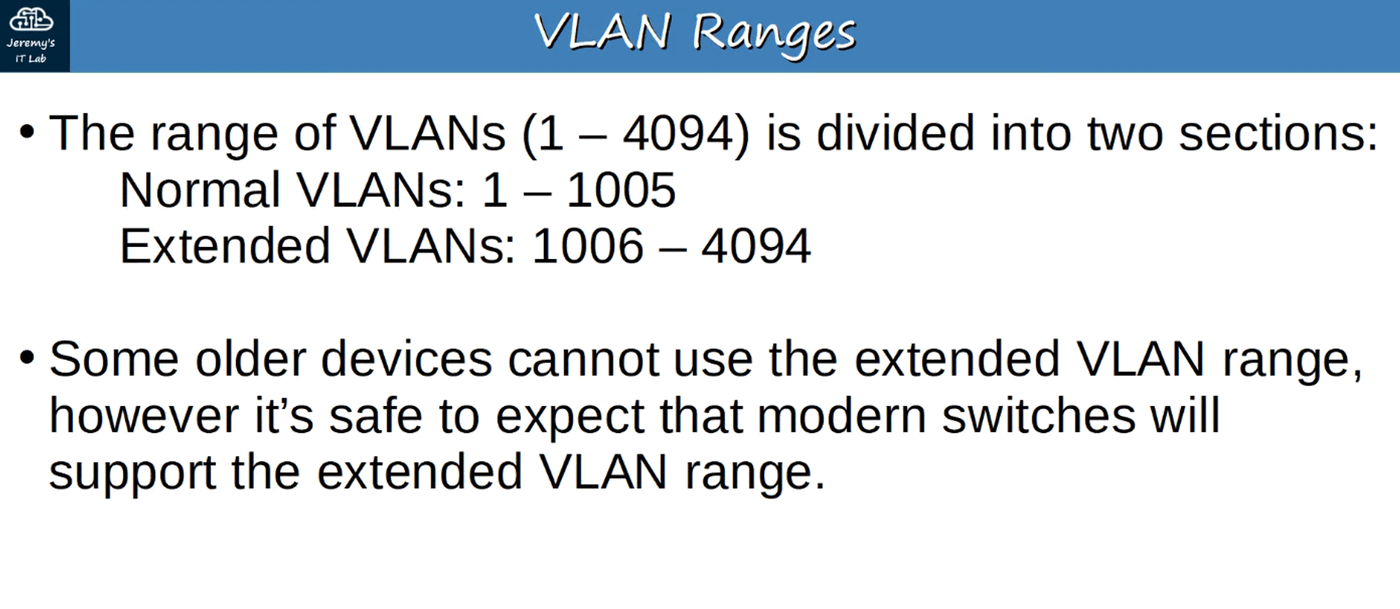
\includegraphics[keepaspectratio,alt={image}]{images/18-vlan-part2/img-007.png}}
\end{figure}

\section{Native VLAN}\label{native-vlan}

\begin{figure}
\centering
\pandocbounded{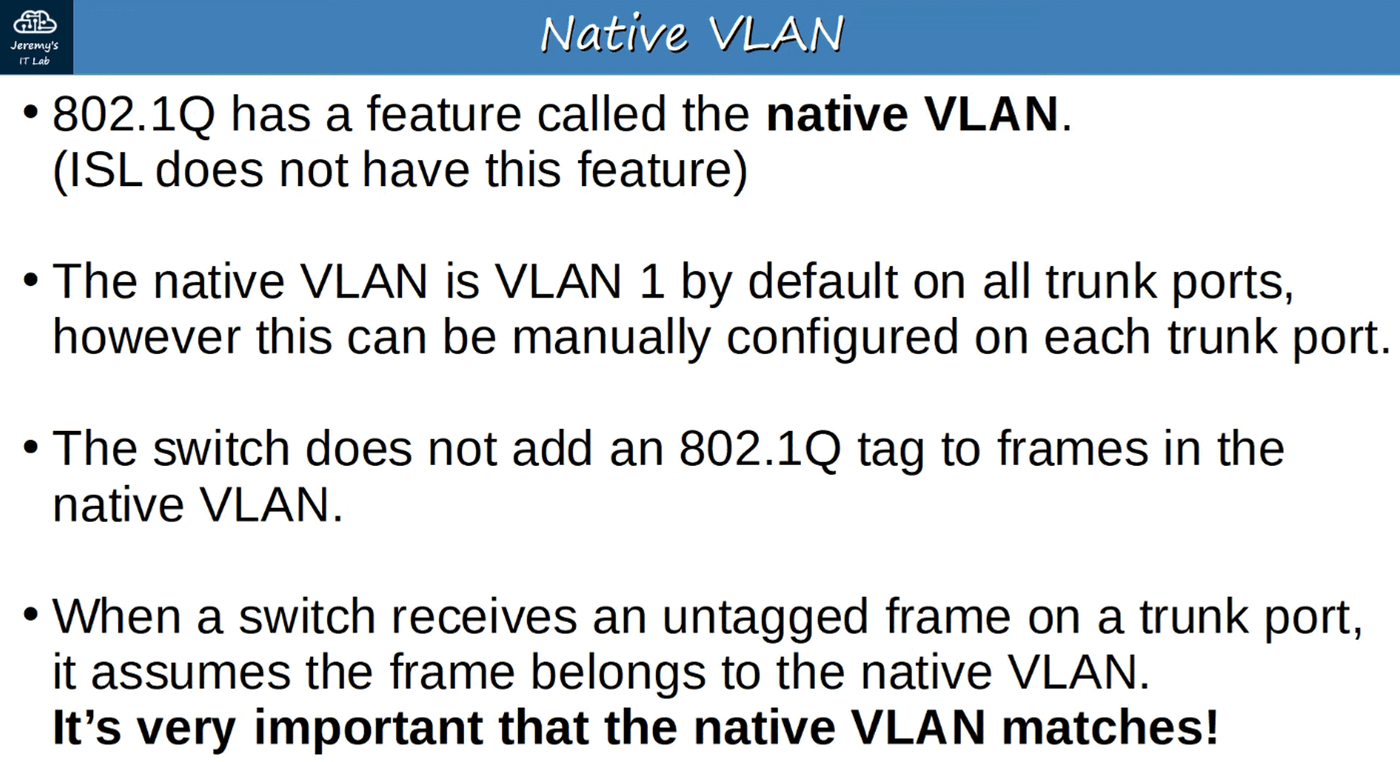
\includegraphics[keepaspectratio,alt={image}]{images/18-vlan-part2/img-008.png}}
\end{figure}

\begin{figure}
\centering
\pandocbounded{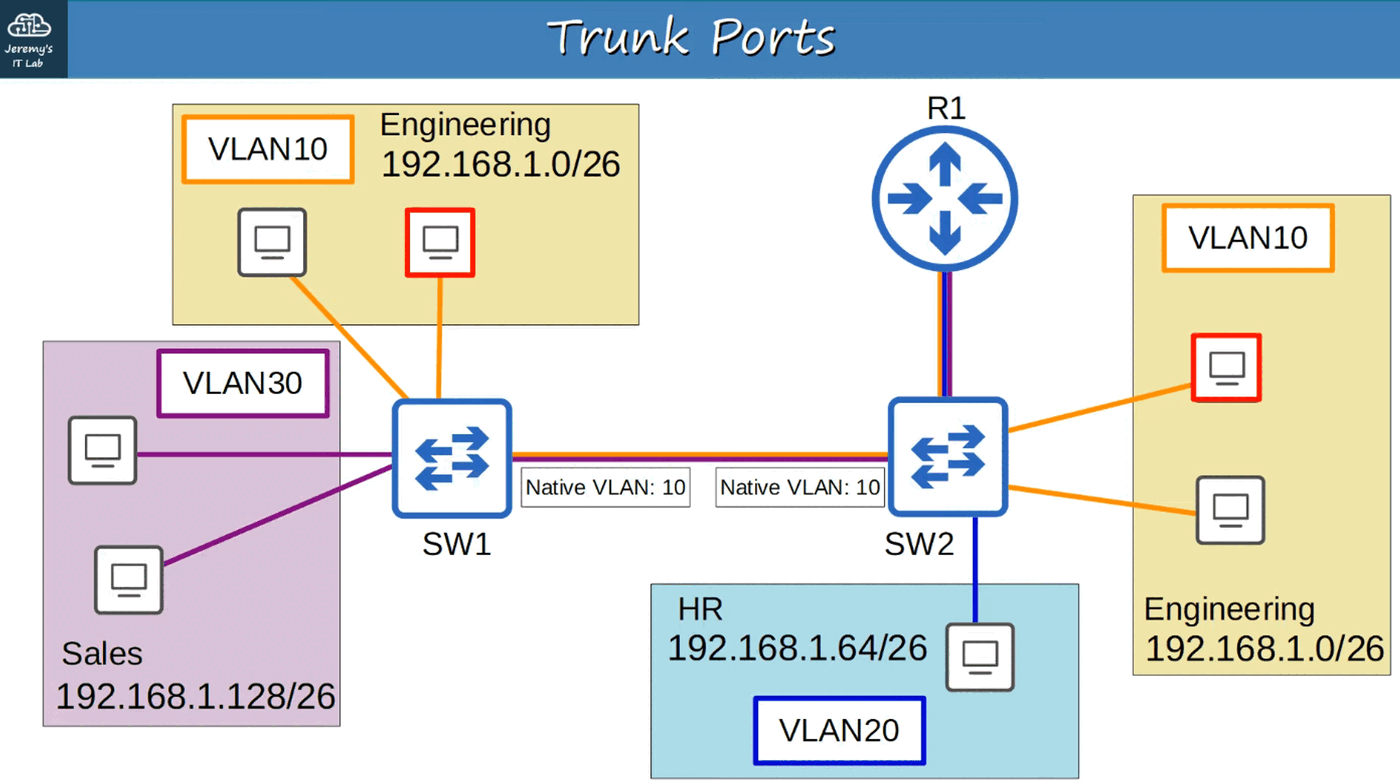
\includegraphics[keepaspectratio,alt={image}]{images/18-vlan-part2/img-009.png}}
\end{figure}

\begin{figure}
\centering
\pandocbounded{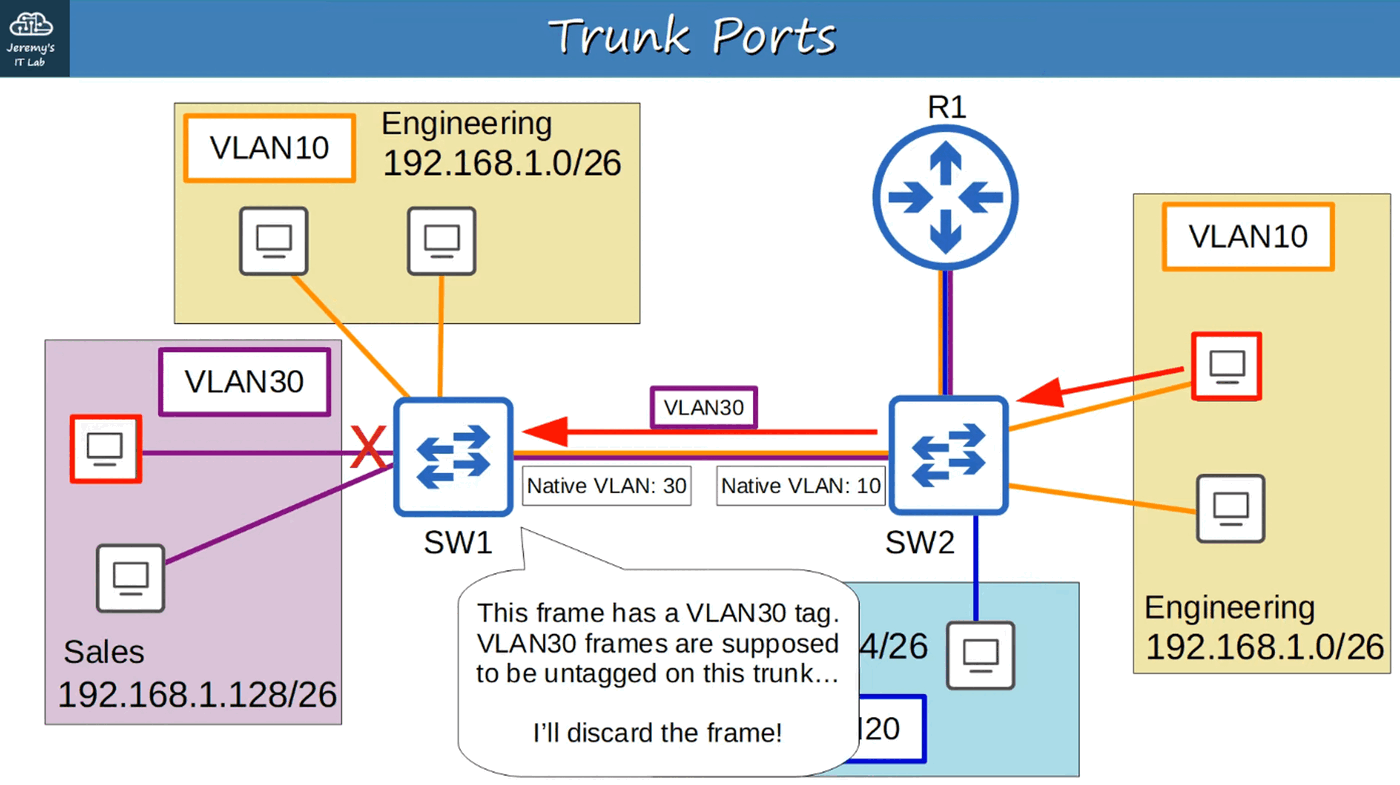
\includegraphics[keepaspectratio,alt={image}]{images/18-vlan-part2/img-010.png}}
\end{figure}

\section{Trunk Configuration}\label{trunk-configuration}

\begin{figure}
\centering
\pandocbounded{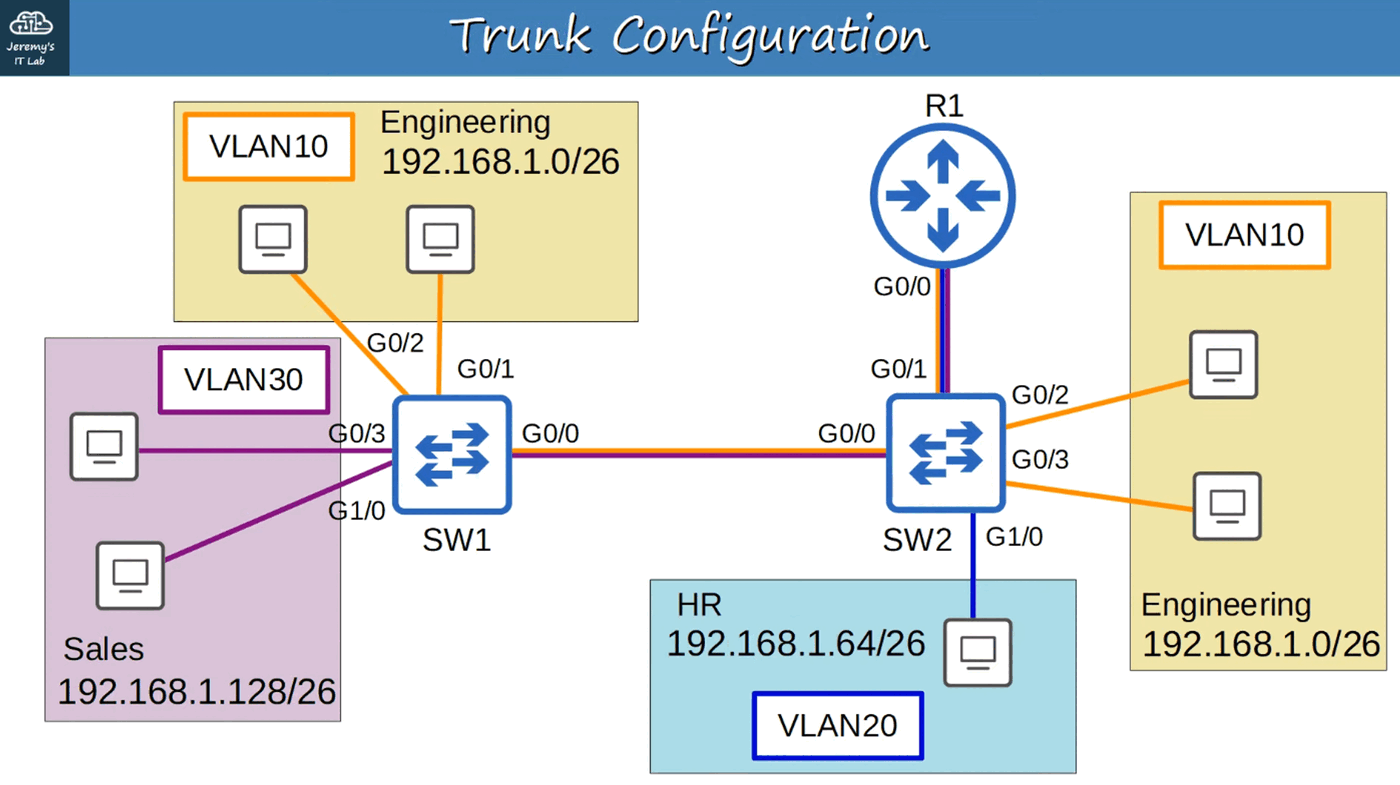
\includegraphics[keepaspectratio,alt={image}]{images/18-vlan-part2/img-011.png}}
\end{figure}

\begin{figure}
\centering
\pandocbounded{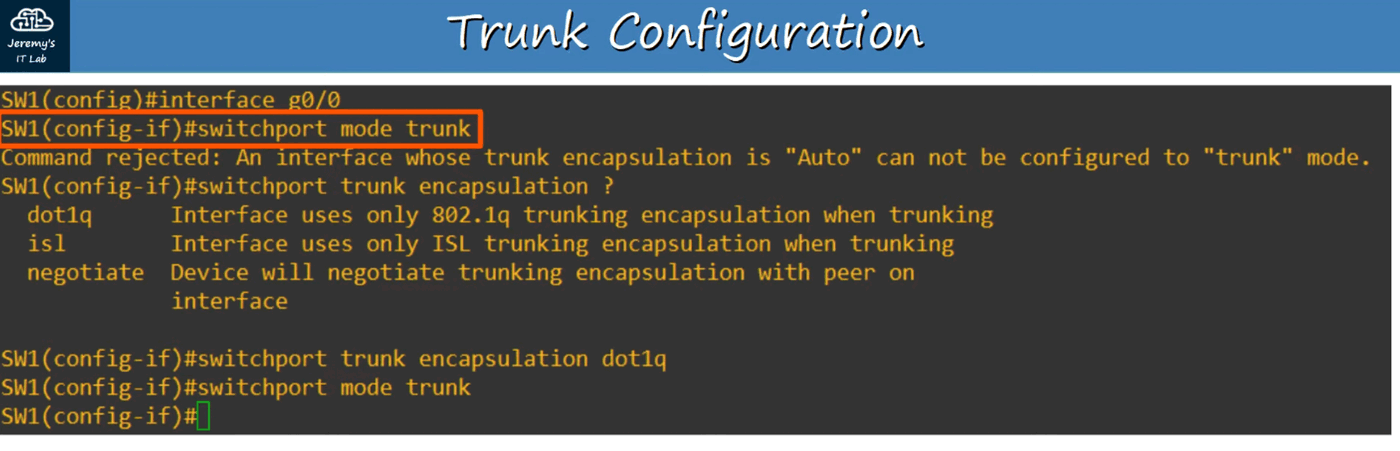
\includegraphics[keepaspectratio,alt={image}]{images/18-vlan-part2/img-012.png}}
\end{figure}

Many modern switches do not support Cisco's ISL at all. They only
support 802.1Q (dot1q)

However, SWITCHES that do support both (like the one I am using in this
example) have a TRUNK encapsulation of ``AUTO'' by default

To MANUALLY configure the INTERFACE as a TRUNK PORT, you must first set
the encapsulation to ``802.1Q'' or ``ISL''. On SWITCHES that only
support 802.1Q, this is not necessary

After you set the encapsulation type, you can then configure the
interface as a TRUNK

\begin{enumerate}
\def\labelenumi{\arabic{enumi})}
\item
  Select the interface to configure
\item
  Use ``\#switchport trunk encapsulation dot1q'' to set the
  encapsulation mode to 802.1Q
\item
  Use ``\#switchport mode trunk'' to manually configure the interface to
  TRUNK
\end{enumerate}

\begin{figure}
\centering
\pandocbounded{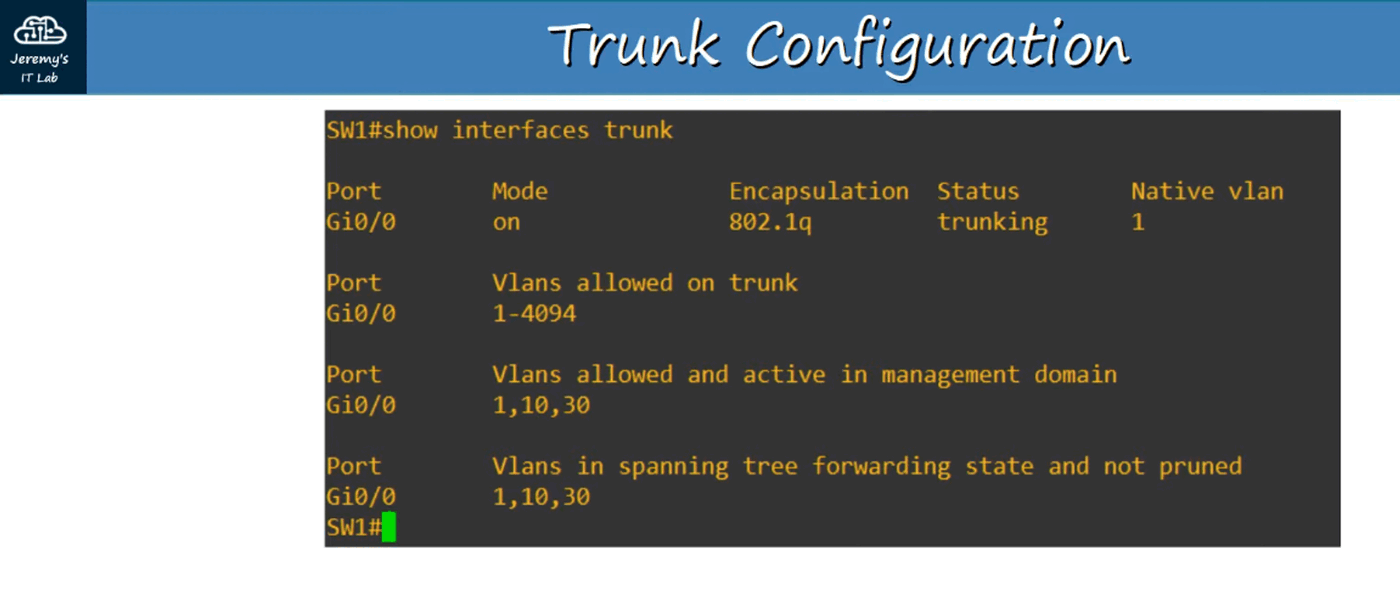
\includegraphics[keepaspectratio,alt={image}]{images/18-vlan-part2/img-013.png}}
\end{figure}

Use the ``\#show interfaces trunk'' command to confirm INTERFACES on
TRUNK

\begin{figure}
\centering
\pandocbounded{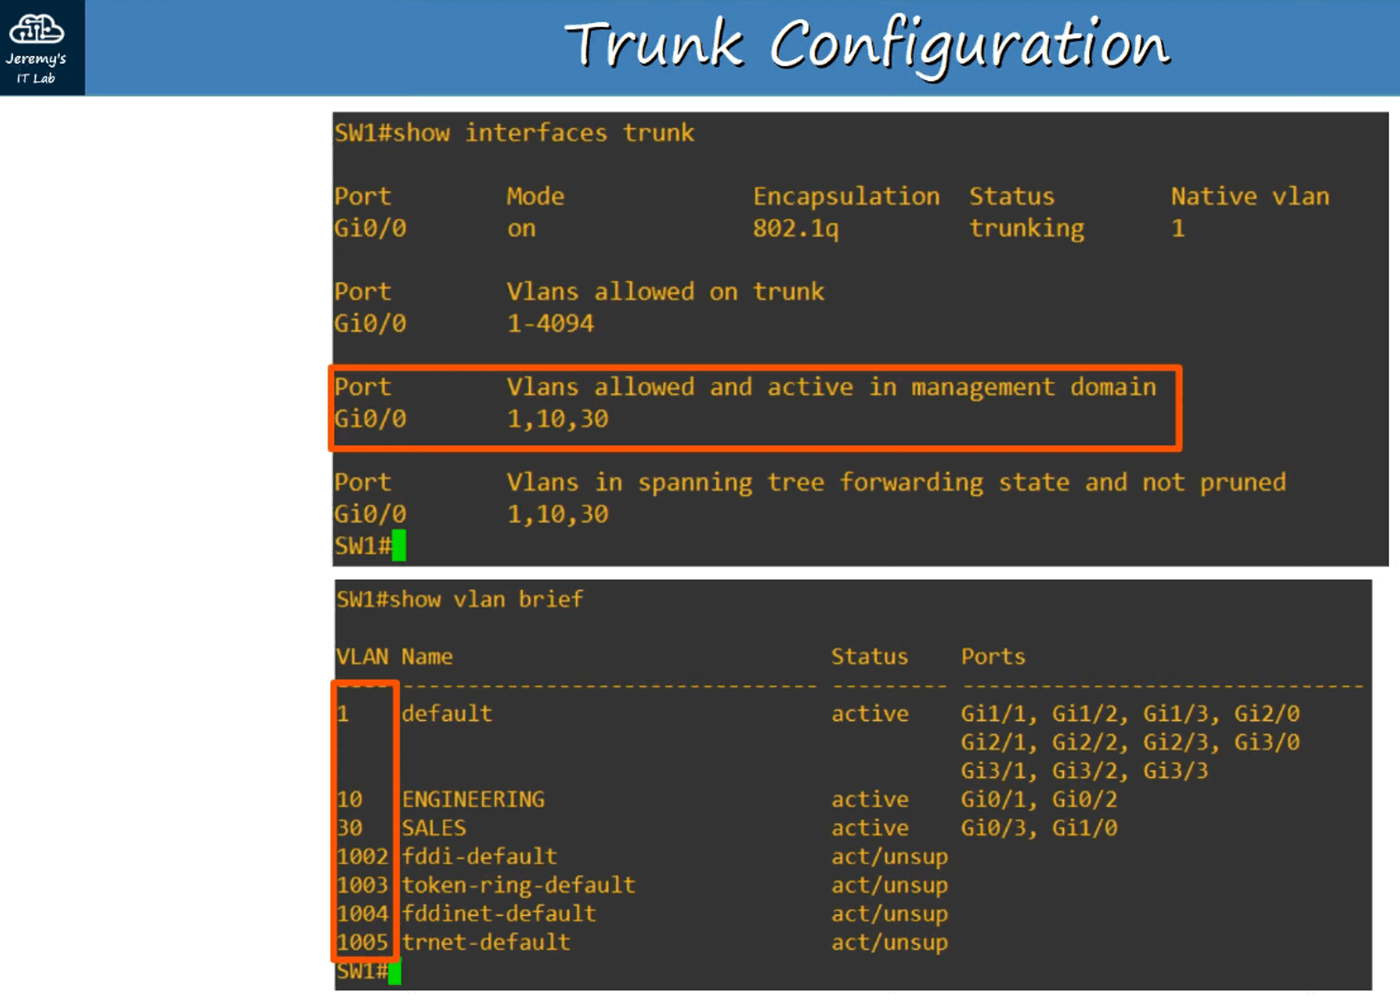
\includegraphics[keepaspectratio,alt={image}]{images/18-vlan-part2/img-014.png}}
\end{figure}

Commands to allow a VLAN on a given TRUNK

\begin{figure}
\centering
\pandocbounded{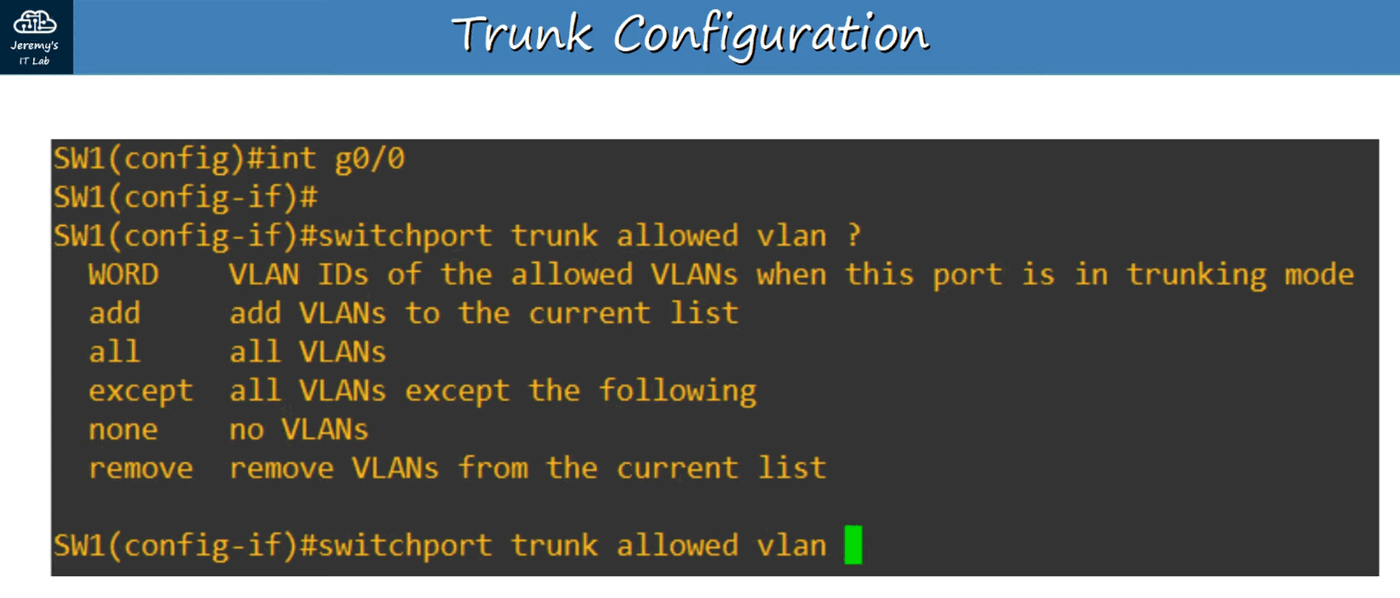
\includegraphics[keepaspectratio,alt={image}]{images/18-vlan-part2/img-015.png}}
\end{figure}

\begin{figure}
\centering
\pandocbounded{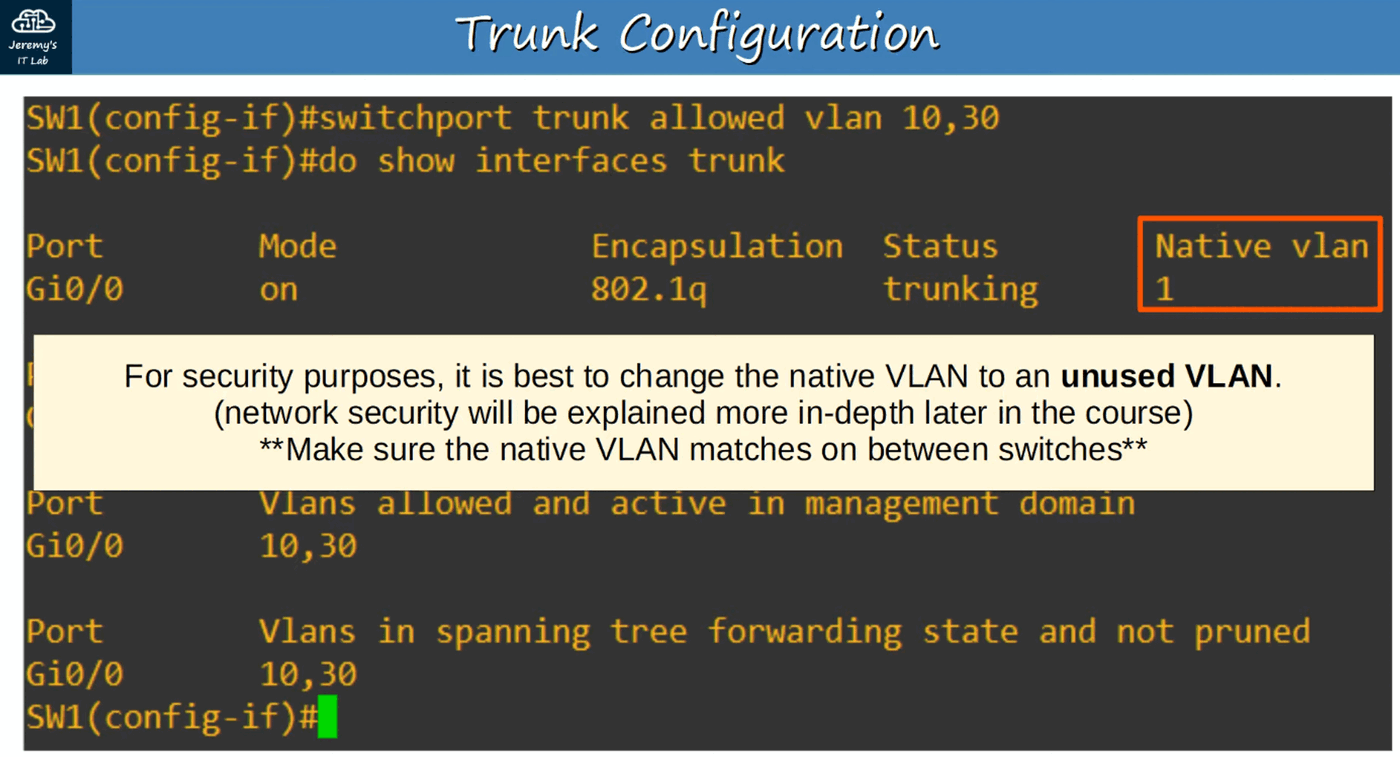
\includegraphics[keepaspectratio,alt={image}]{images/18-vlan-part2/img-016.png}}
\end{figure}

Command to change the NATIVE VLAN

\begin{figure}
\centering
\pandocbounded{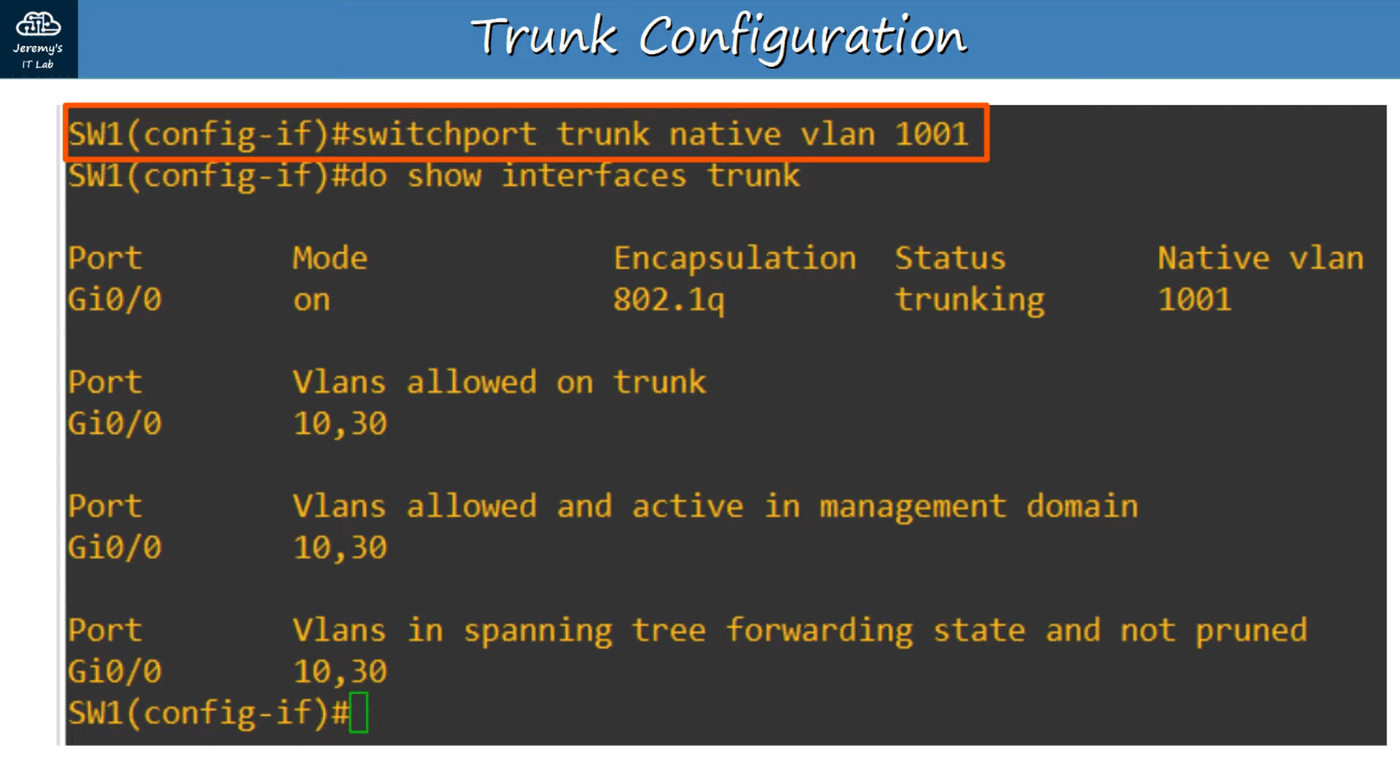
\includegraphics[keepaspectratio,alt={image}]{images/18-vlan-part2/img-017.png}}
\end{figure}

\begin{figure}
\centering
\pandocbounded{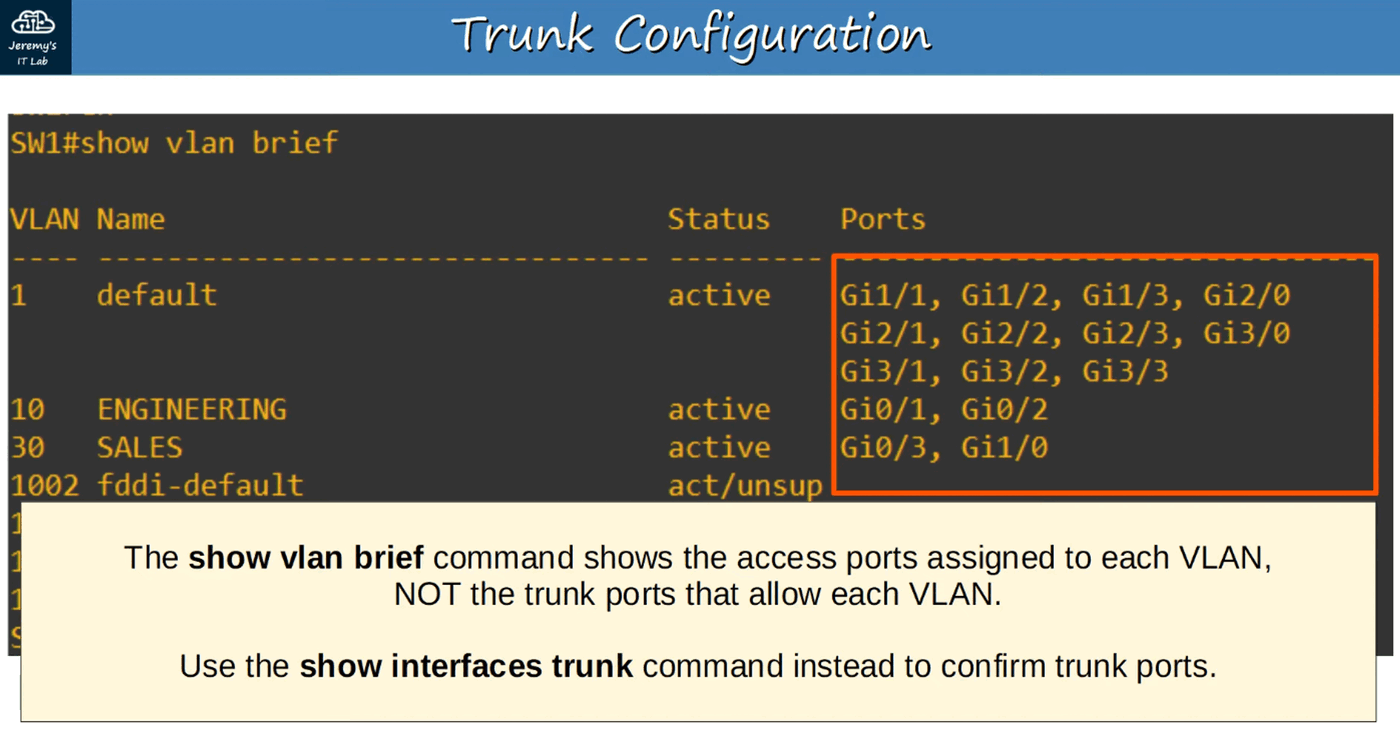
\includegraphics[keepaspectratio,alt={image}]{images/18-vlan-part2/img-018.png}}
\end{figure}

Setting up our TRUNKS for this Network

\begin{figure}
\centering
\pandocbounded{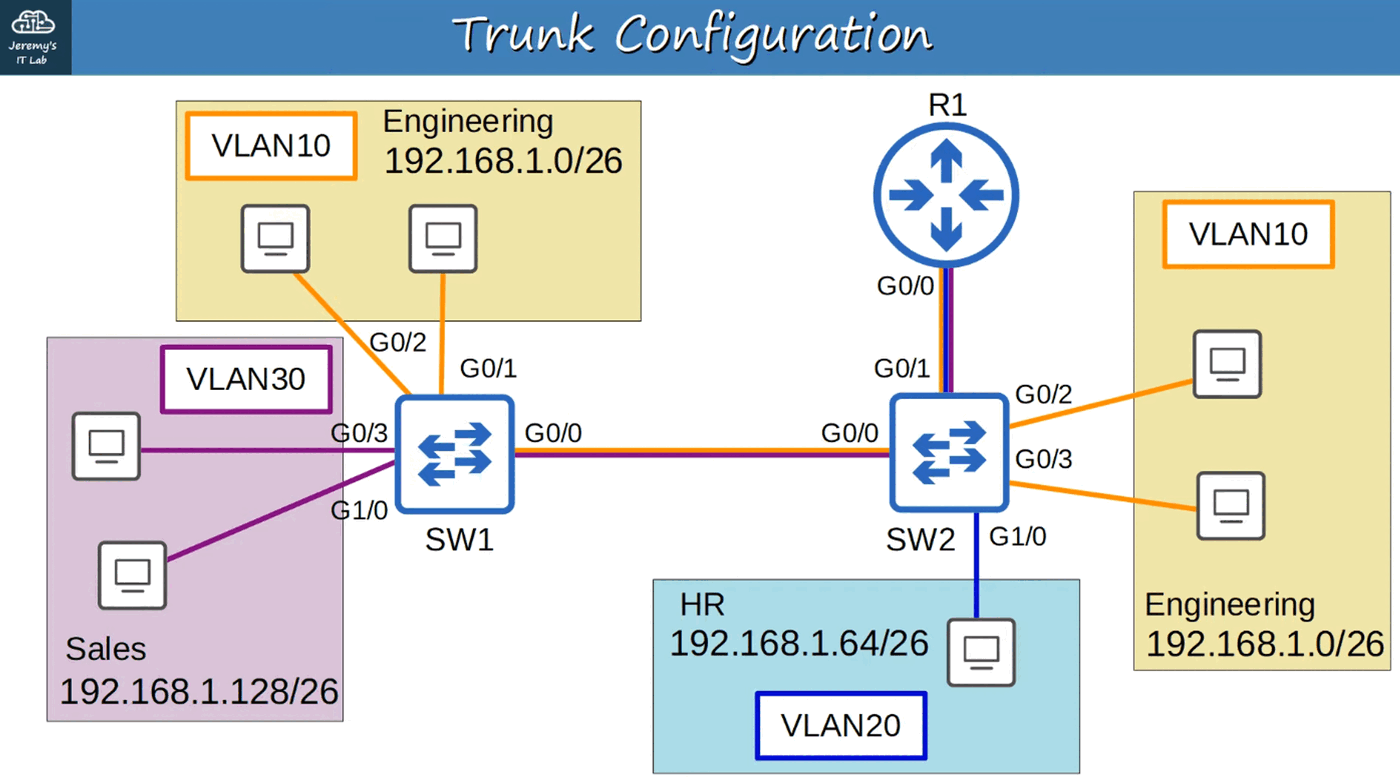
\includegraphics[keepaspectratio,alt={image}]{images/18-vlan-part2/img-019.png}}
\end{figure}

We will need to configure :

SW1 : g0/0 interface (already configure above this section)

SW2: g0/0, and g0/1 interface

SW2 g0/0

\begin{figure}
\centering
\pandocbounded{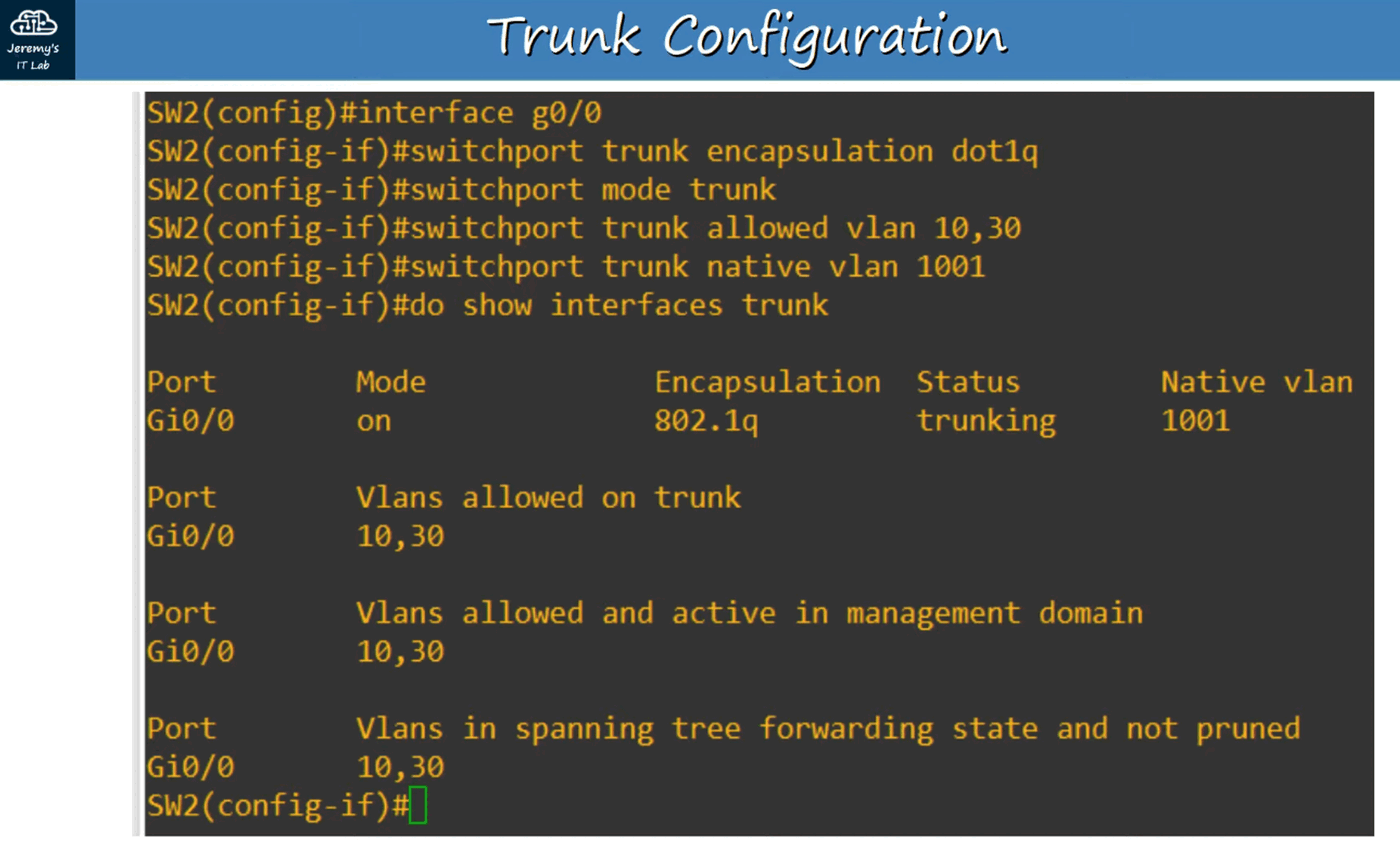
\includegraphics[keepaspectratio,alt={image}]{images/18-vlan-part2/img-020.png}}
\end{figure}

SW2 g0/1

\begin{figure}
\centering
\pandocbounded{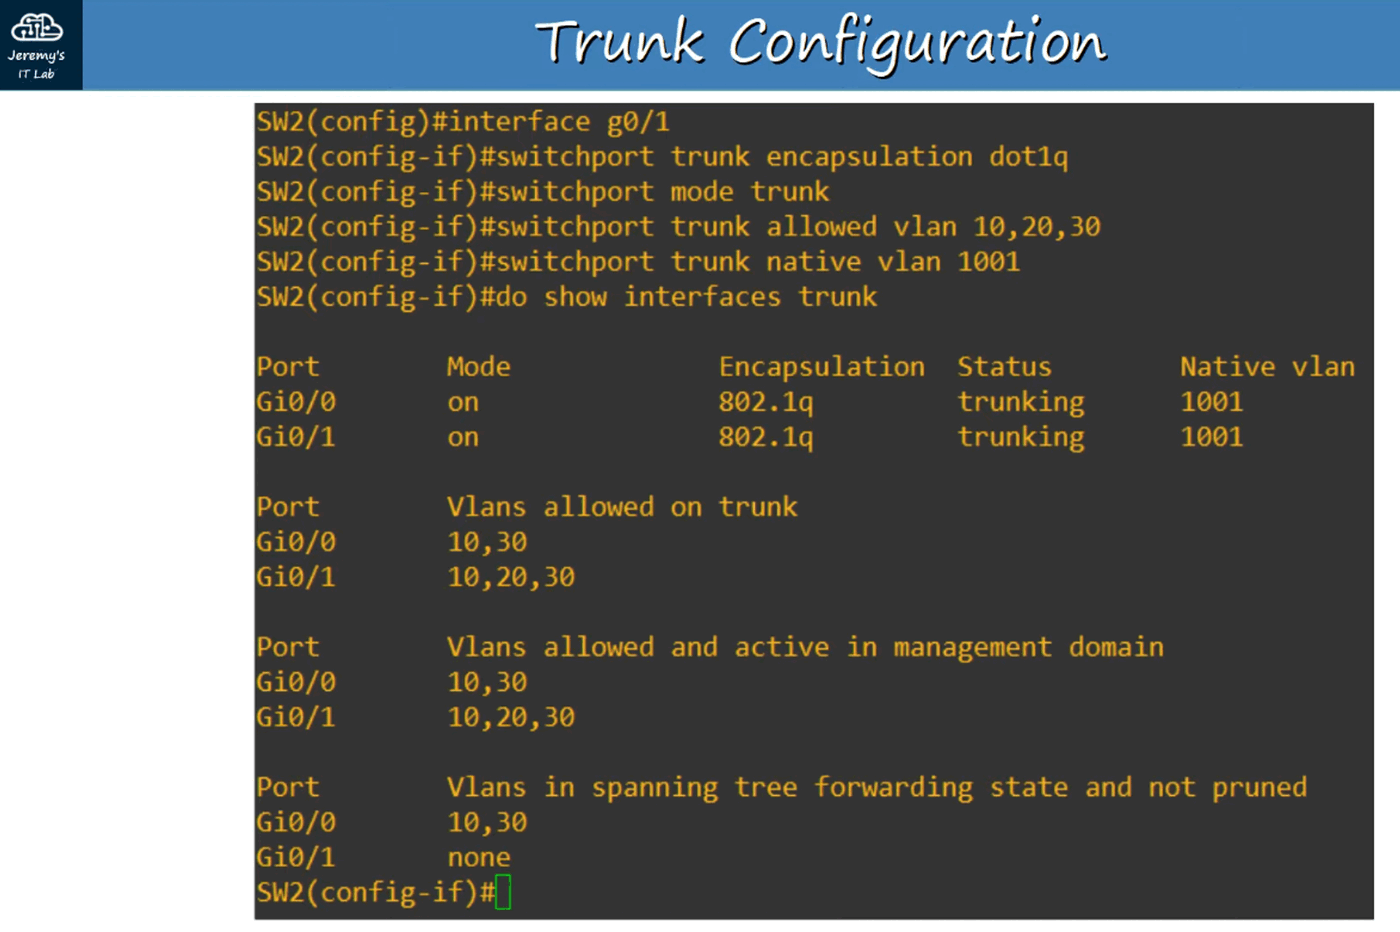
\includegraphics[keepaspectratio,alt={image}]{images/18-vlan-part2/img-021.png}}
\end{figure}

What about the ROUTER, R1 ?

\section{Router on a Stick (ROAS)}\label{router-on-a-stick-roas}

\begin{figure}
\centering
\pandocbounded{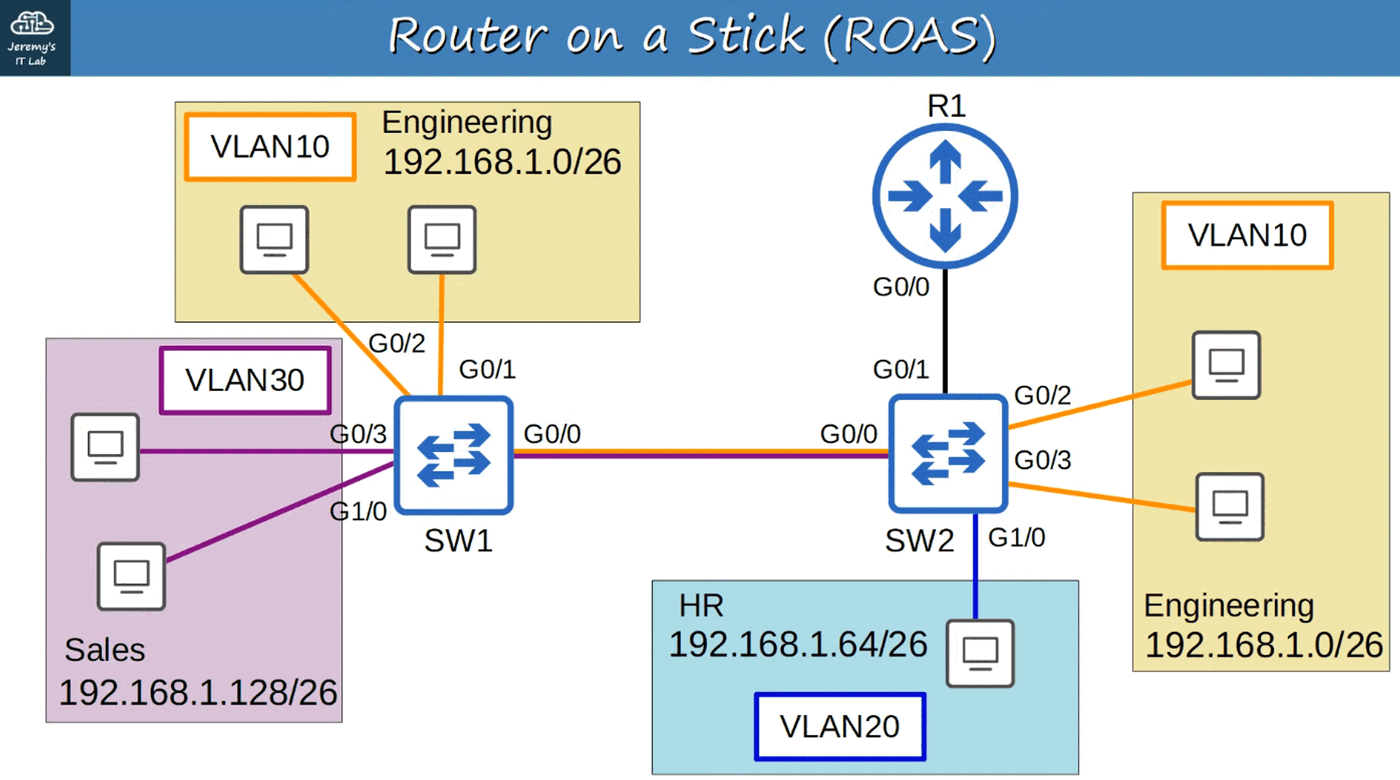
\includegraphics[keepaspectratio,alt={image}]{images/18-vlan-part2/img-022.png}}
\end{figure}

\begin{figure}
\centering
\pandocbounded{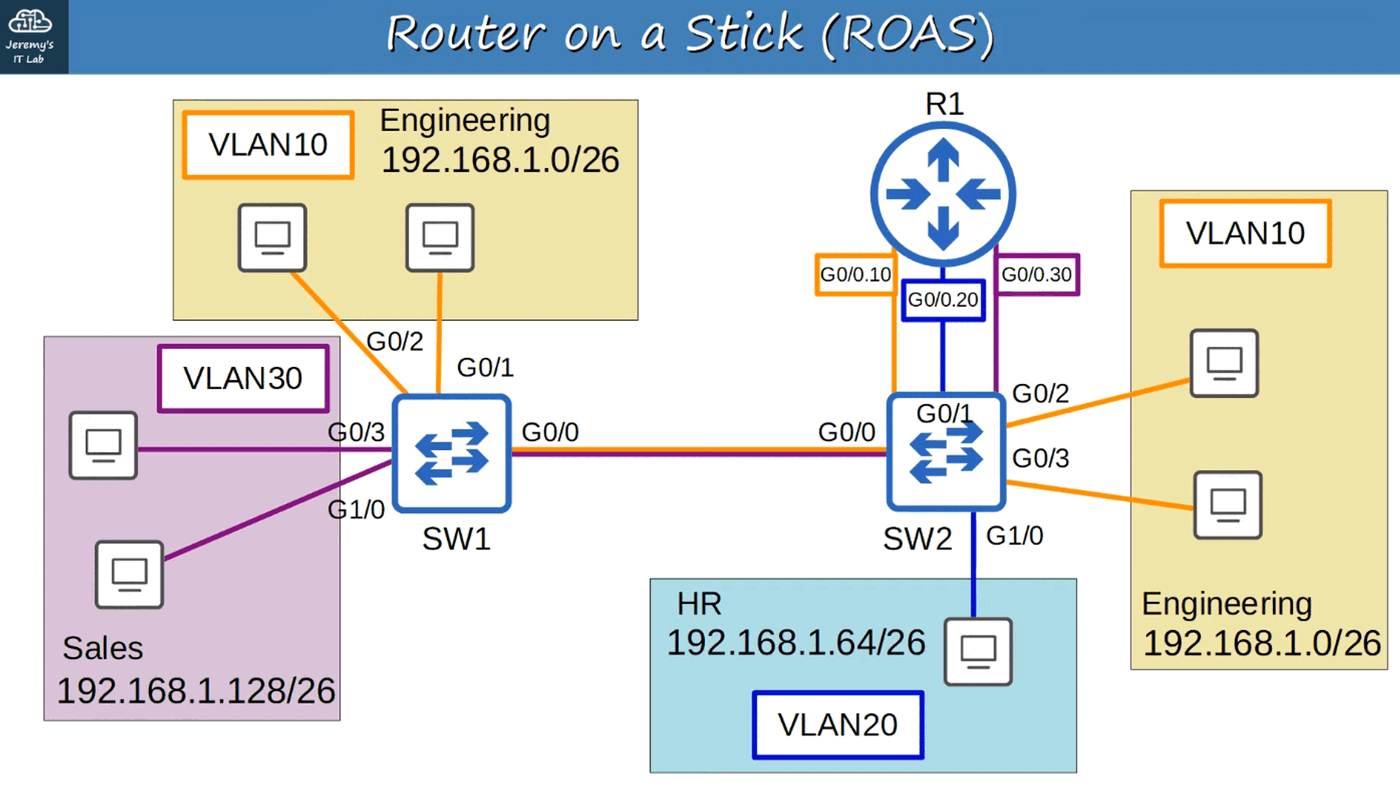
\includegraphics[keepaspectratio,alt={image}]{images/18-vlan-part2/img-023.png}}
\end{figure}

\begin{figure}
\centering
\pandocbounded{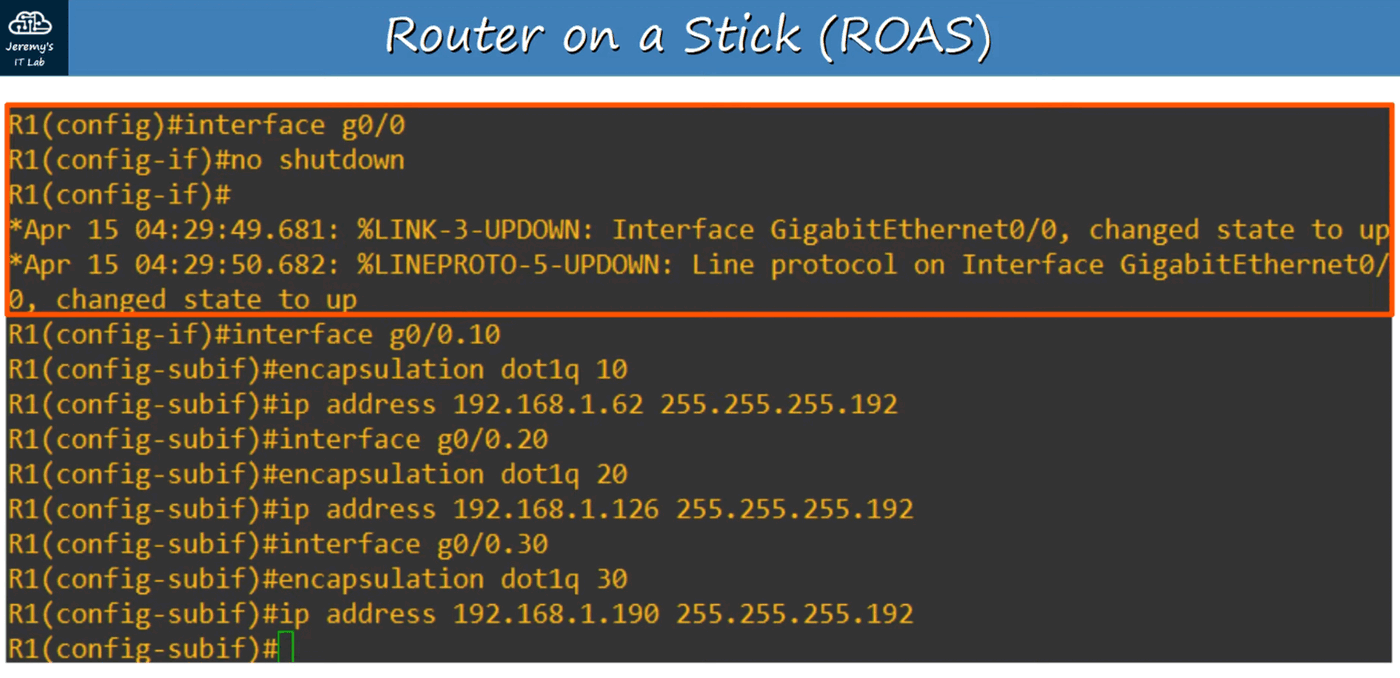
\includegraphics[keepaspectratio,alt={image}]{images/18-vlan-part2/img-024.png}}
\end{figure}

NOTE the Sub-Interface names (like the network diagram) of 0.10, 0.20
and 0.30

You assign them IP addresses identically like you would a regular
interface (using the last usable IP address of a given VLAN subnet)

Sub-interfaces will appear with the ``show ip interface brief'' command

\begin{figure}
\centering
\pandocbounded{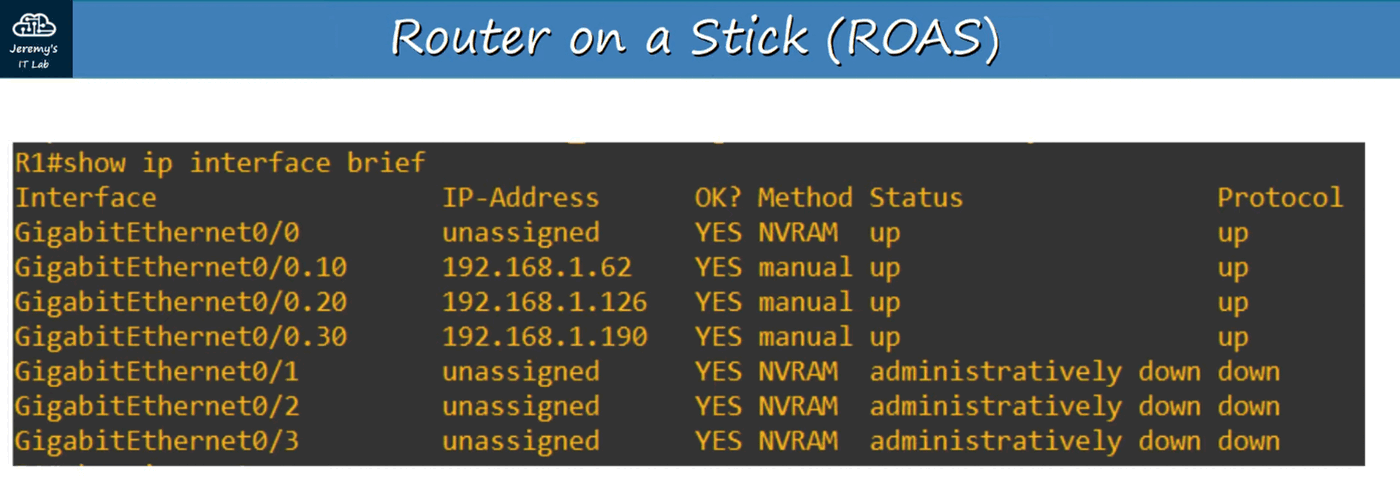
\includegraphics[keepaspectratio,alt={image}]{images/18-vlan-part2/img-025.png}}
\end{figure}

They also appear in the ``show ip route'' command (Route Table)

\begin{figure}
\centering
\pandocbounded{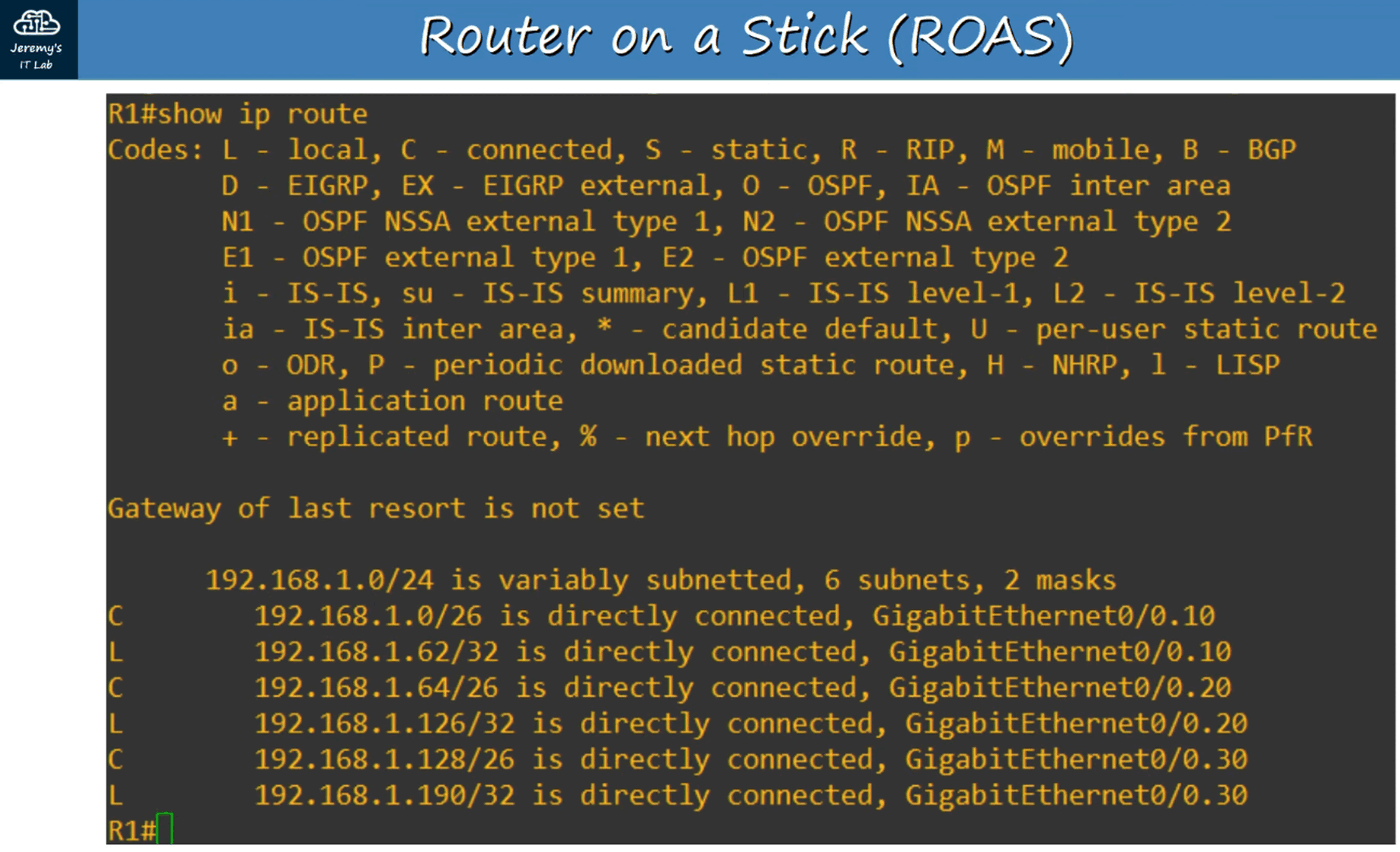
\includegraphics[keepaspectratio,alt={image}]{images/18-vlan-part2/img-026.png}}
\end{figure}

ROAS is used to route between multiple VLANs using a SINGLE interface on
a ROUTER and SWITCH

The SWITCH interface is configured as a regular TRUNK

The ROUTER interface is configured using SUB-INTERFACES. You configure
the VLAN tag and IP address on EACH SUB-INTERFACE

The ROUTER will behave as if frames arriving with a certain VLAN tag
have arrived on the SUB-INTERFACE configured with that VLAN tag

The ROUTER will TAG frames sent out of EACH SUB-INTERFACE with the VLAN
TAG configured on the SUB-INTERFACE

\chapter{VLANs: Part 3}\label{vlans-part-3}

\section{Native VLAN on a Router
(ROAS)}\label{native-vlan-on-a-router-roas}

\begin{figure}
\centering
\pandocbounded{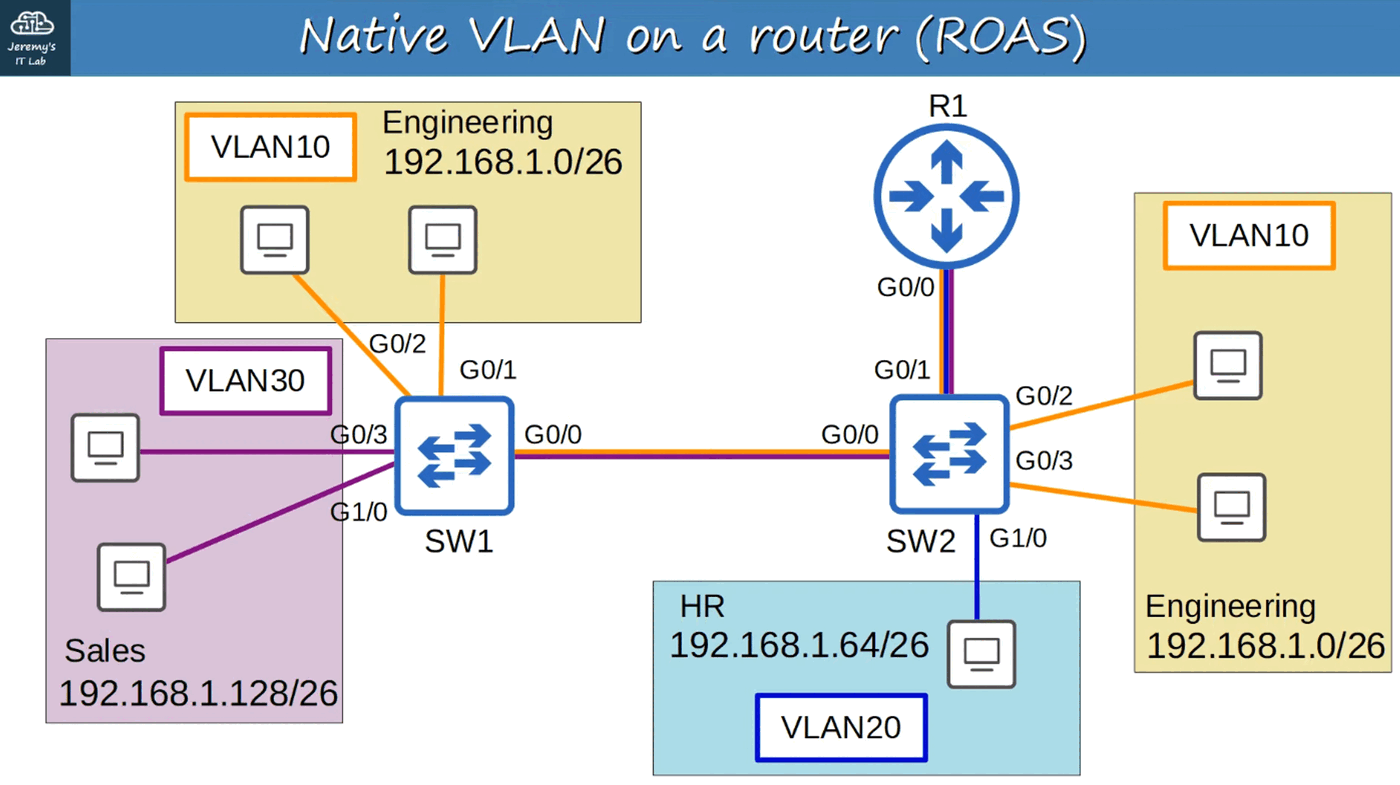
\includegraphics[keepaspectratio,alt={image}]{images/19-vlan-part3/img-001.png}}
\end{figure}

Native VLAN untagged frames are faster and more efficient (smaller) than
tagged ones.

Let's reset all SWITCHES (SW1 and SW2) to native vlan 10

\begin{figure}
\centering
\pandocbounded{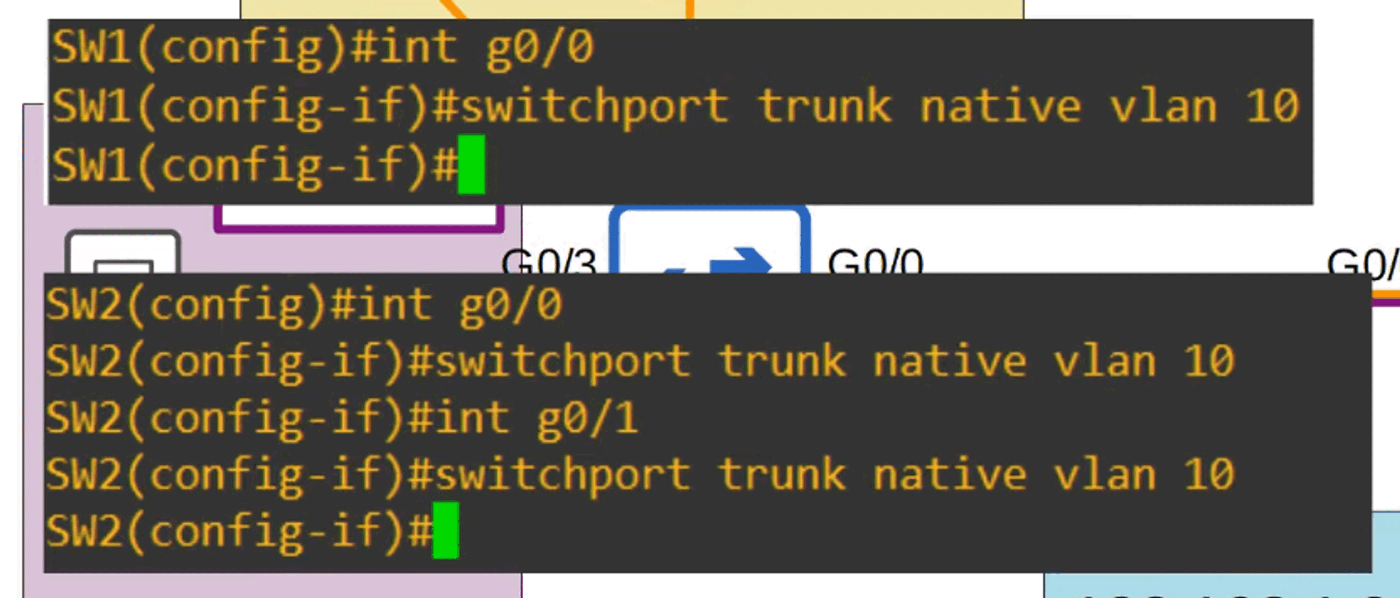
\includegraphics[keepaspectratio,alt={image}]{images/19-vlan-part3/img-002.png}}
\end{figure}

There are \textbf{TWO methods} of configuring the native VLAN on a
router:

\begin{itemize}
\tightlist
\item
  Use the command ``encapsulation dot1q \textless vlan-id\textgreater''
  on a Sub-Interface
\end{itemize}

\begin{figure}
\centering
\pandocbounded{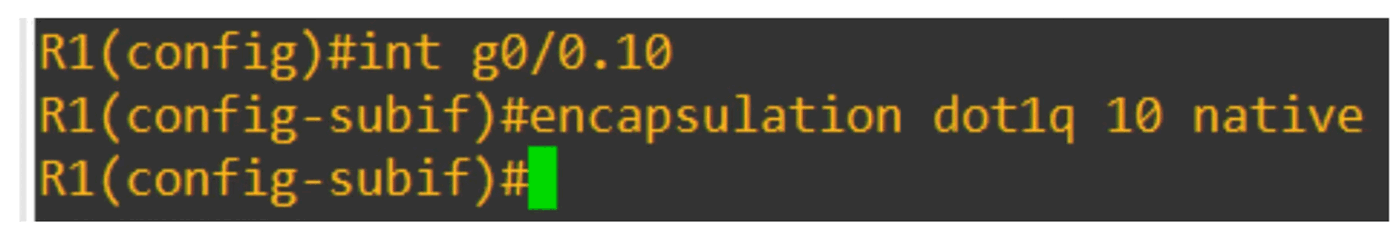
\includegraphics[keepaspectratio,alt={image}]{images/19-vlan-part3/img-003.png}}
\end{figure}

OR

\begin{itemize}
\tightlist
\item
  Configure the IP address for the native VLAN on the router's physical
  interface (the ``\textbf{encapsulation dot1q}
  \textless vlan-id\textgreater{} command is not necessary''
\end{itemize}

\begin{figure}
\centering
\pandocbounded{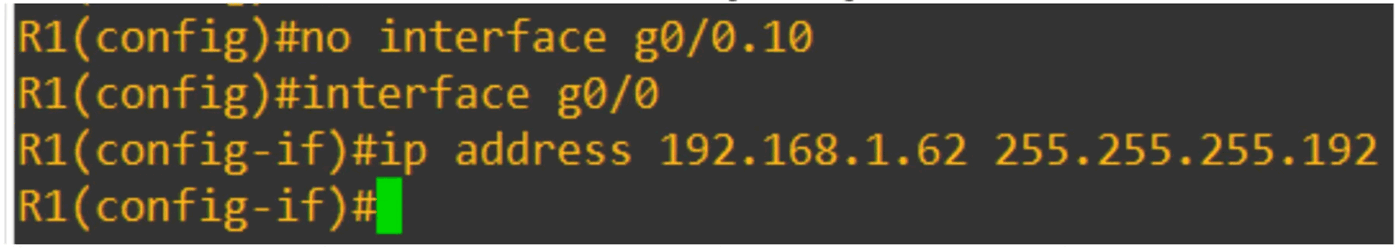
\includegraphics[keepaspectratio,alt={image}]{images/19-vlan-part3/img-004.png}}
\end{figure}

Output of ``show running-config'' of G0/0 Interface

\begin{figure}
\centering
\pandocbounded{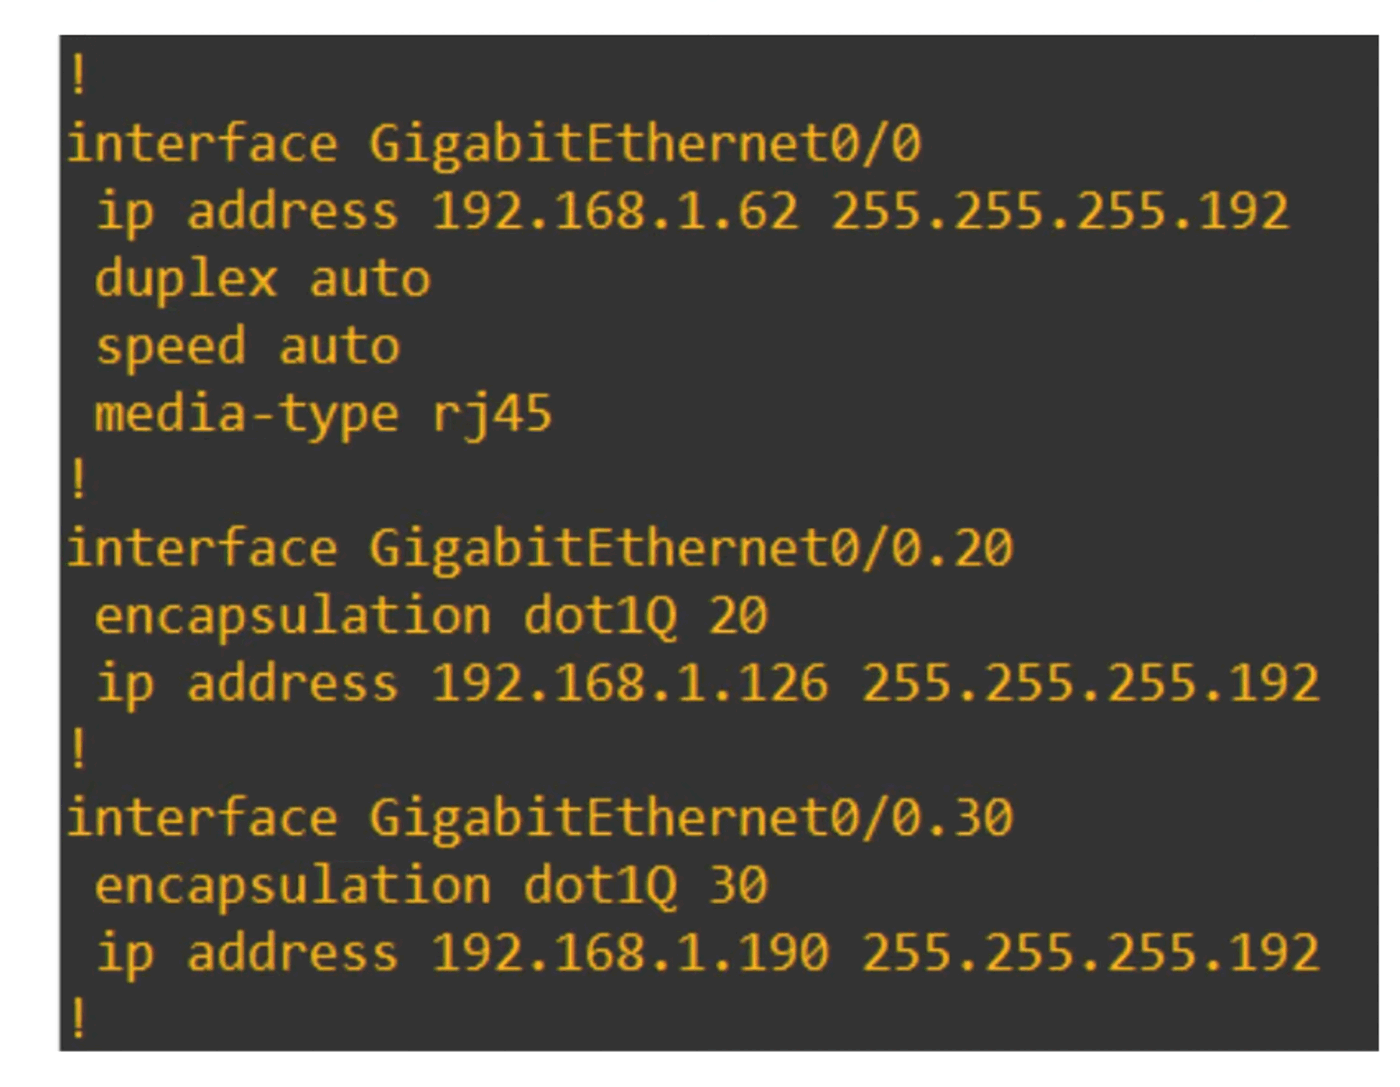
\includegraphics[keepaspectratio,alt={image}]{images/19-vlan-part3/img-005.png}}
\end{figure}

\section{Layer 3 (Multilayer)
Switches}\label{layer-3-multilayer-switches}

\section{Icon Appearance}\label{icon-appearance}

\begin{figure}
\centering
\pandocbounded{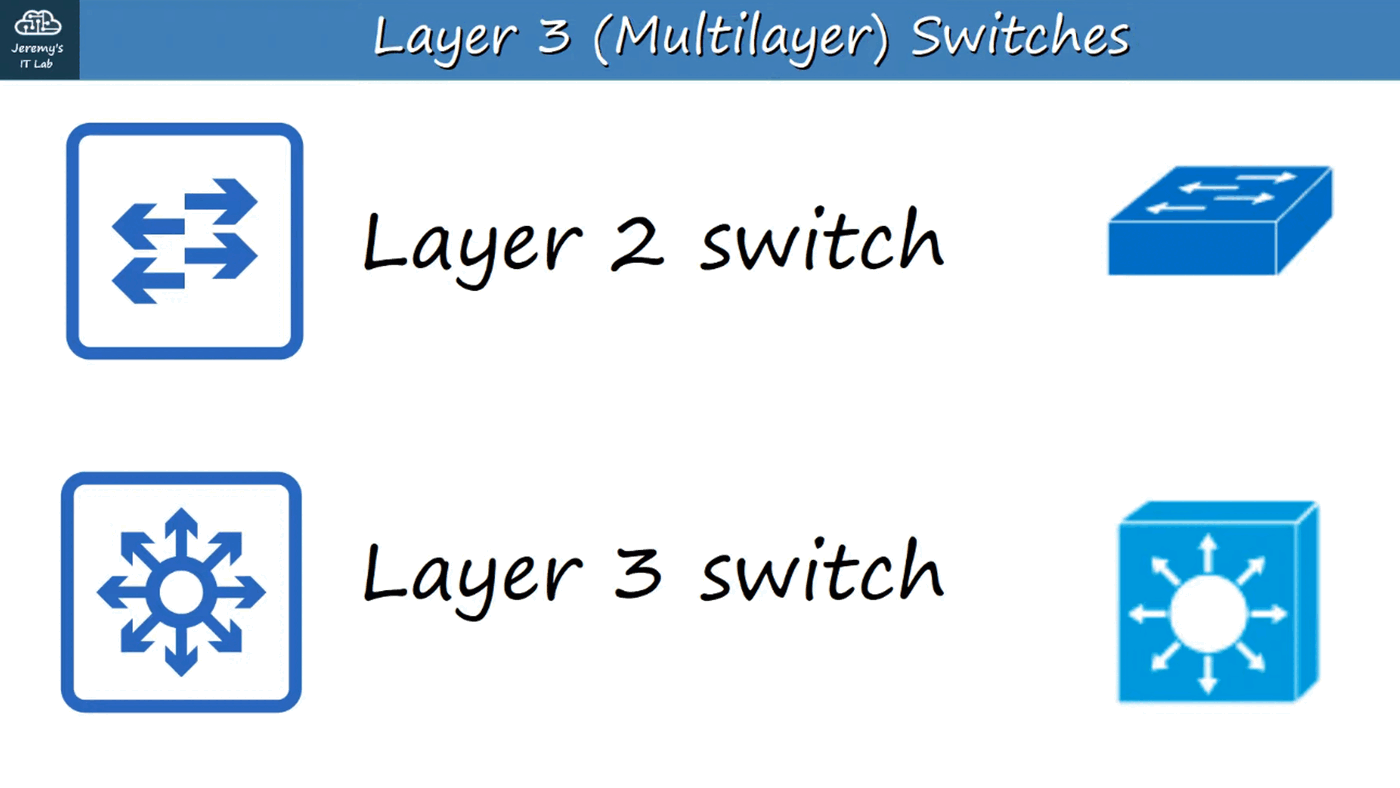
\includegraphics[keepaspectratio,alt={image}]{images/19-vlan-part3/img-006.png}}
\end{figure}

\begin{itemize}
\tightlist
\item
  A MULTILAYER SWITCH is capable of both SWITCHING and ROUTING
\item
  It is LAYER 3 AWARE
\item
  You can assign IP Addresses to its L3 Virtual Interface, like a router
\item
  You can create Virtual Interfaces for each VLAN, and assign IP
  addresses to those interfaces
\item
  You can configure routes on it, just like a ROUTER
\item
  It can be used for inter-VLAN routing
\end{itemize}

\begin{figure}
\centering
\pandocbounded{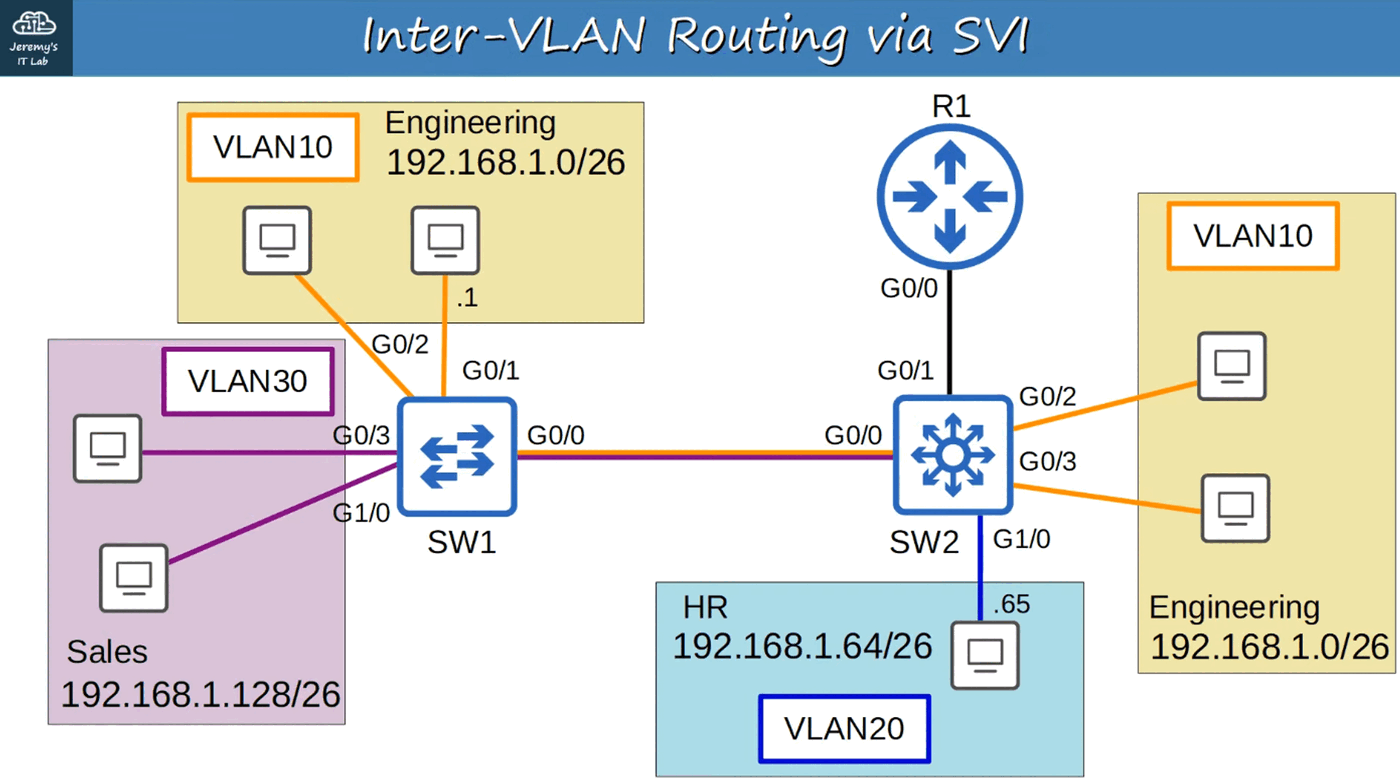
\includegraphics[keepaspectratio,alt={image}]{images/19-vlan-part3/img-007.png}}
\end{figure}

SW2 Replaced with a Layer 3 Switch

Multi-VLAN connections to R1 removed and replaced with a point-to-point
Layer 3 connection

\begin{figure}
\centering
\pandocbounded{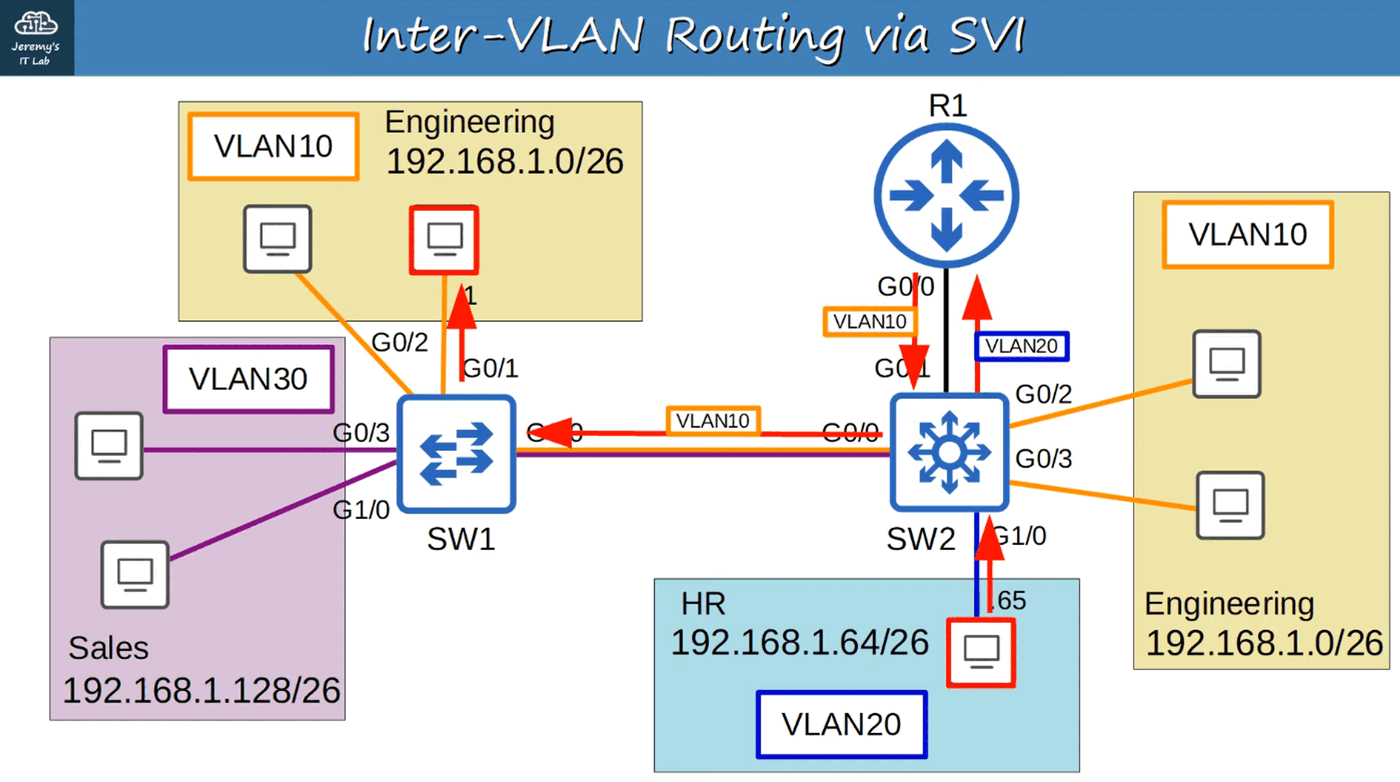
\includegraphics[keepaspectratio,alt={image}]{images/19-vlan-part3/img-008.png}}
\end{figure}

\begin{itemize}
\tightlist
\item
  SVIs (Switch Virtual Interfaces) are the virtual interfaces you can
  assign IP addresses to in a MULTILAYER SWITCH.
\item
  Configure each HOST to use the SVI (NOT the ROUTER R1) as their
  Gateway Address
\item
  To send traffic to different SUBNETS / VLANS, the PCs will send
  traffic to the SWITCH, and the SWITCH will route the traffic.
\end{itemize}

\begin{figure}
\centering
\pandocbounded{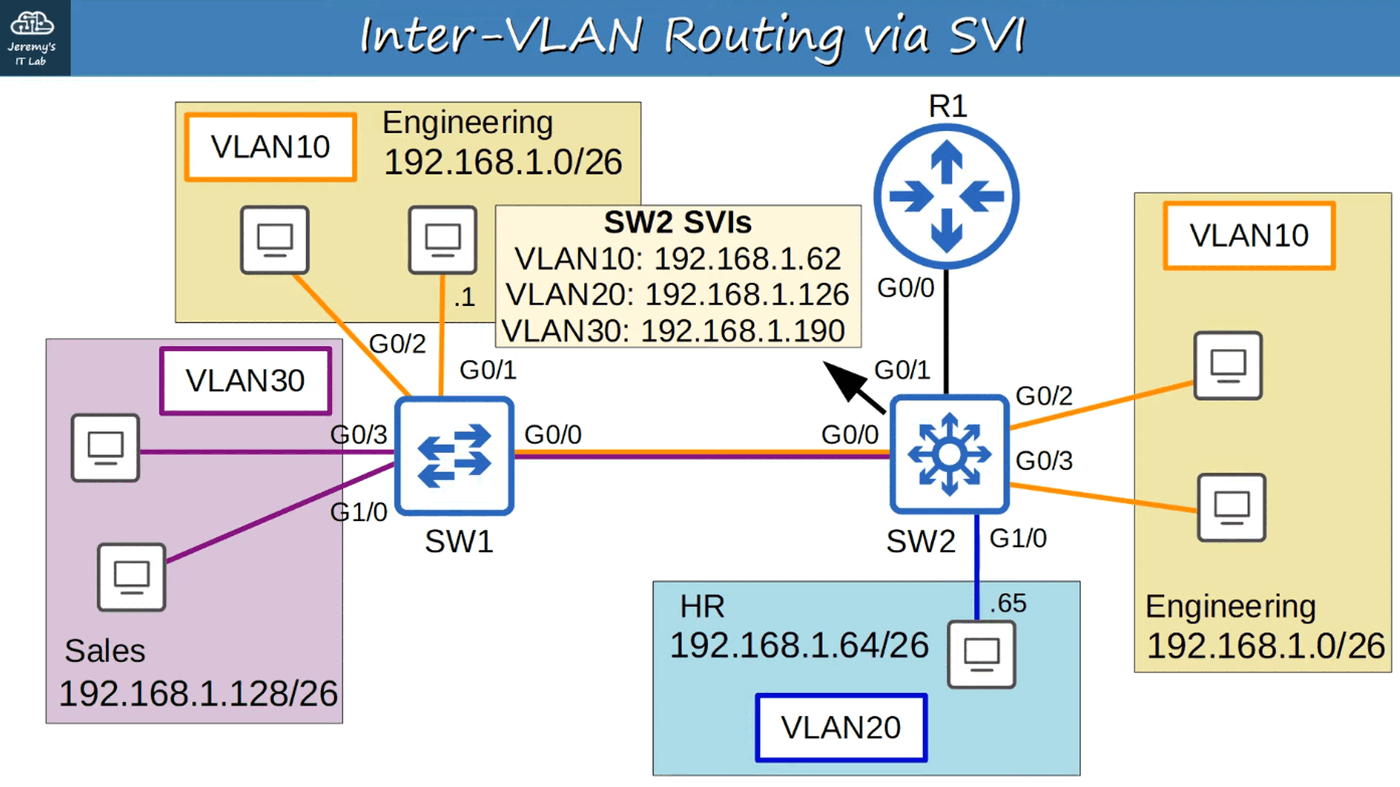
\includegraphics[keepaspectratio,alt={image}]{images/19-vlan-part3/img-009.png}}
\end{figure}

\begin{figure}
\centering
\pandocbounded{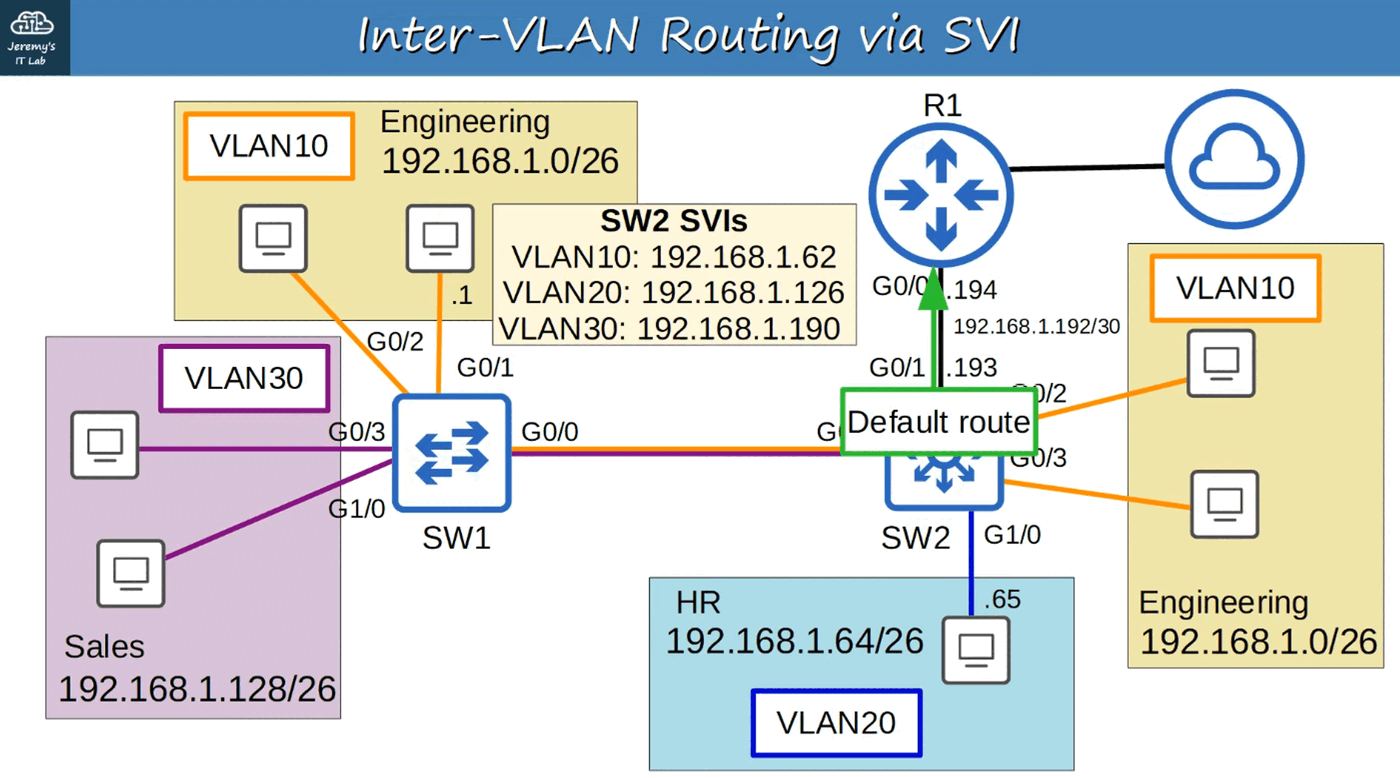
\includegraphics[keepaspectratio,alt={image}]{images/19-vlan-part3/img-010.png}}
\end{figure}

Clearing R1 configuration to set to work with the Layer 3 Point-to-Point
connection

\begin{figure}
\centering
\pandocbounded{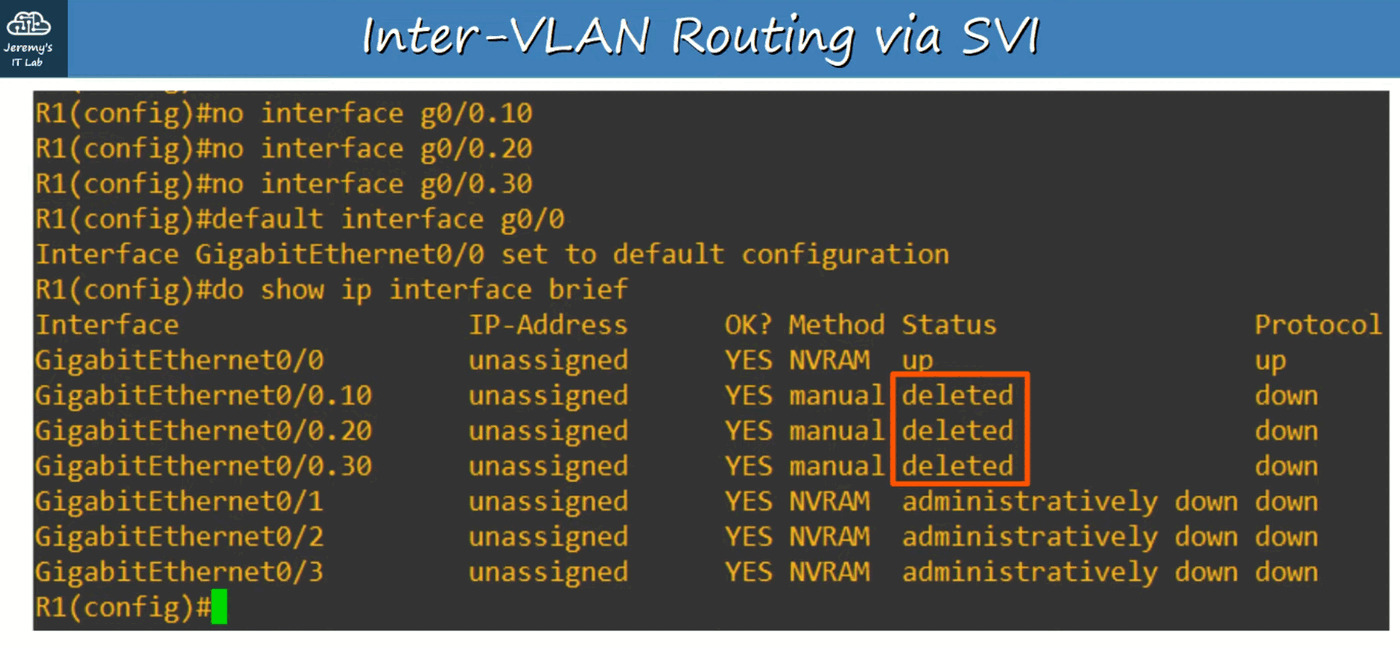
\includegraphics[keepaspectratio,alt={image}]{images/19-vlan-part3/img-011.png}}
\end{figure}

\#no interface \textless sub-interface id\textgreater{} : removes the
VLAN interface

\#default interface g0/0 : resets the g0/0 interface to it's default
settings

Then configure the default R1 G0/0 interface's to IP address :
192.168.1.194 (as per the network diagram)

Configuration of SW2 to use SVI and the Layer 3 Point-to-Point
connection with R1

\begin{figure}
\centering
\pandocbounded{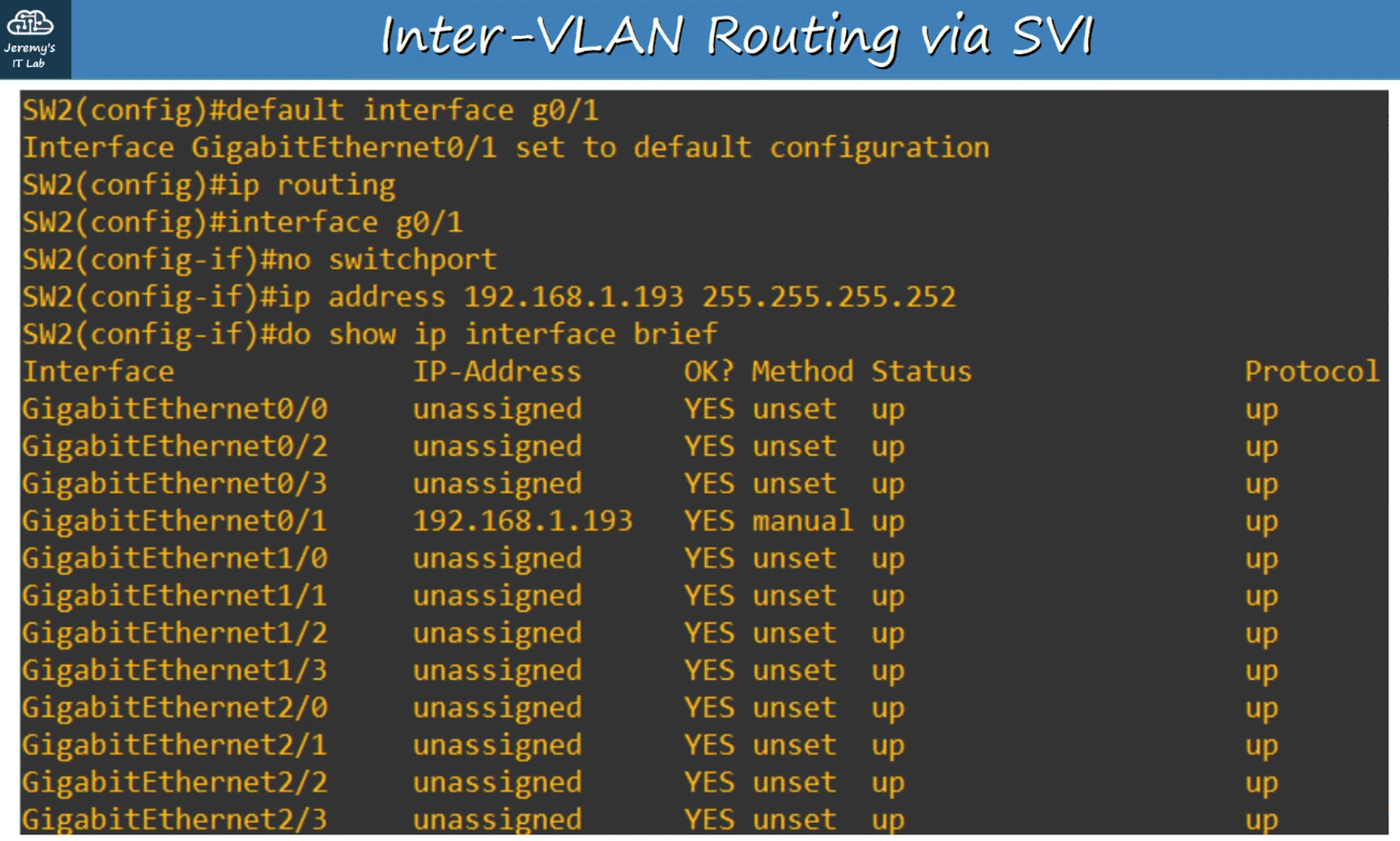
\includegraphics[keepaspectratio,alt={image}]{images/19-vlan-part3/img-012.png}}
\end{figure}

``default interface \textless interface-id\textgreater'' : resets
settings on specified interface to defaults

``ip routing'' : \textbf{IMPORTANT} command to enable Layer 3 routing on
the SWITCH

``no switchport'' : configures the interface from a Layer 2 Switchport
to a Layer 3 ``routed port''

The sets the Default Route to R1 (192.168.1.194) so that all traffic
leaving the network gets routed through R1's Gateway of Last Resort (aka
The Default Gateway)

\begin{figure}
\centering
\pandocbounded{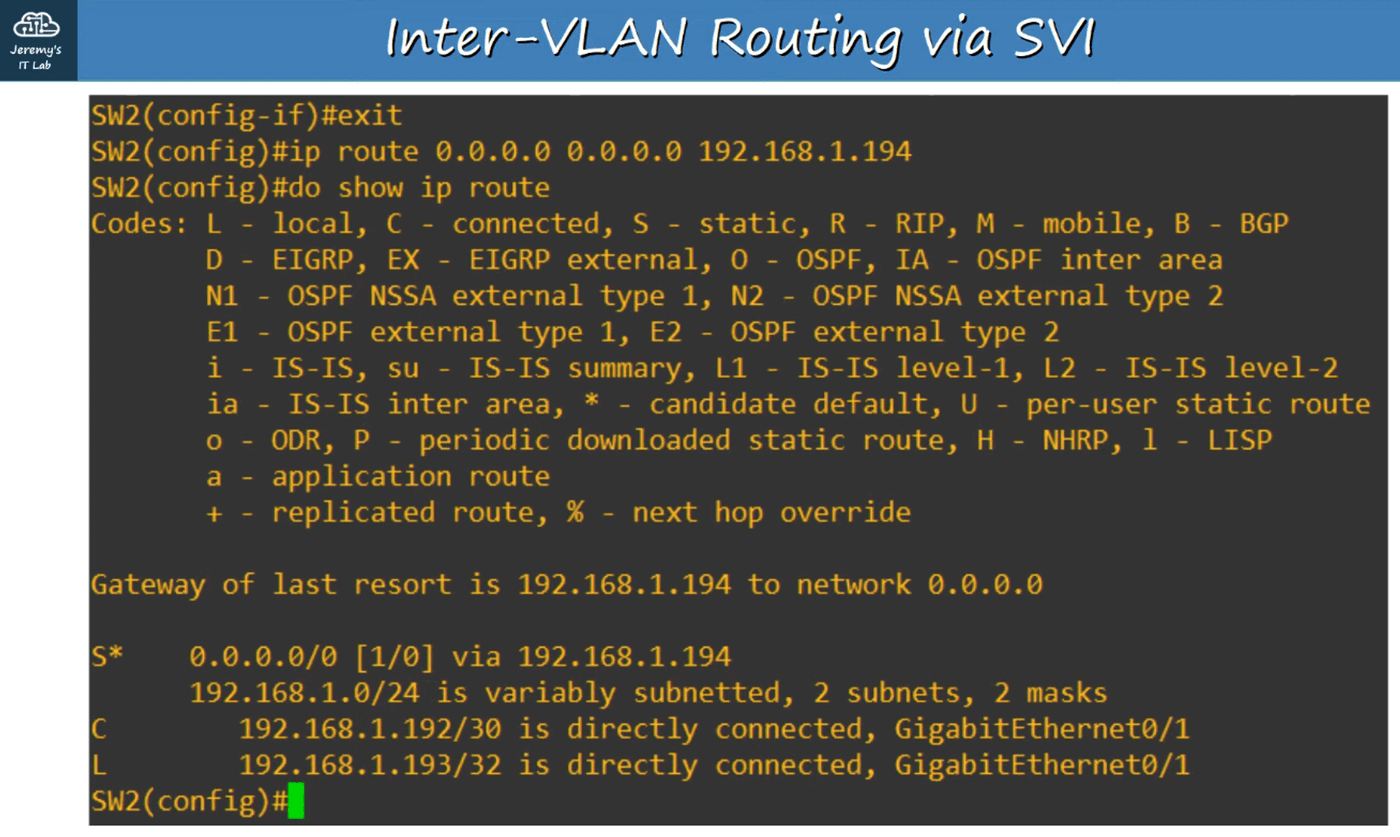
\includegraphics[keepaspectratio,alt={image}]{images/19-vlan-part3/img-013.png}}
\end{figure}

\begin{figure}
\centering
\pandocbounded{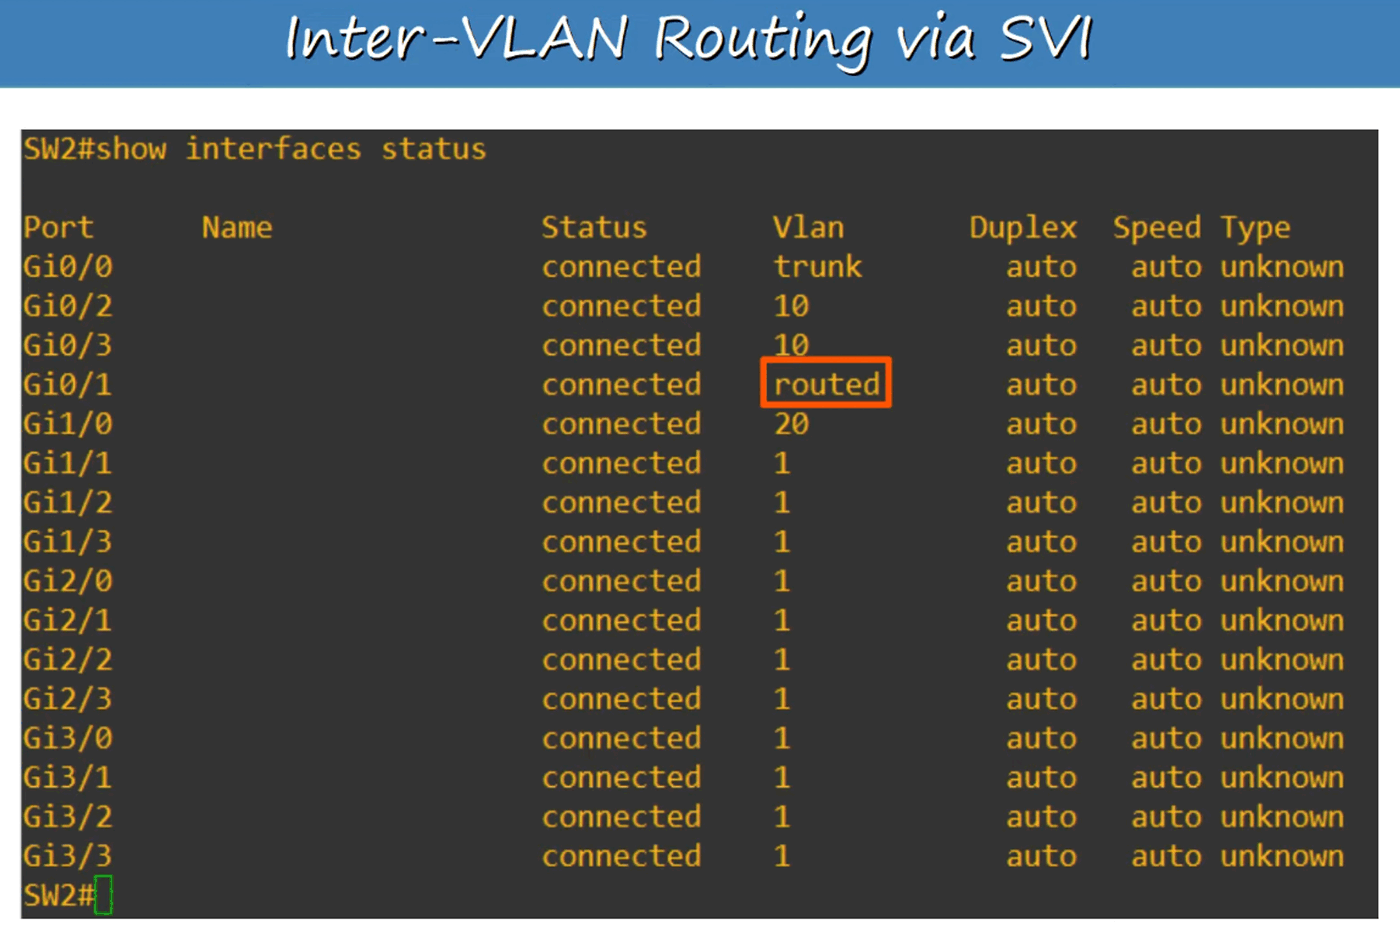
\includegraphics[keepaspectratio,alt={image}]{images/19-vlan-part3/img-014.png}}
\end{figure}

SVI CONFIGURATION ON SW2 (Virtual LAYER 3 ROUTING INTERFACES)

\begin{figure}
\centering
\pandocbounded{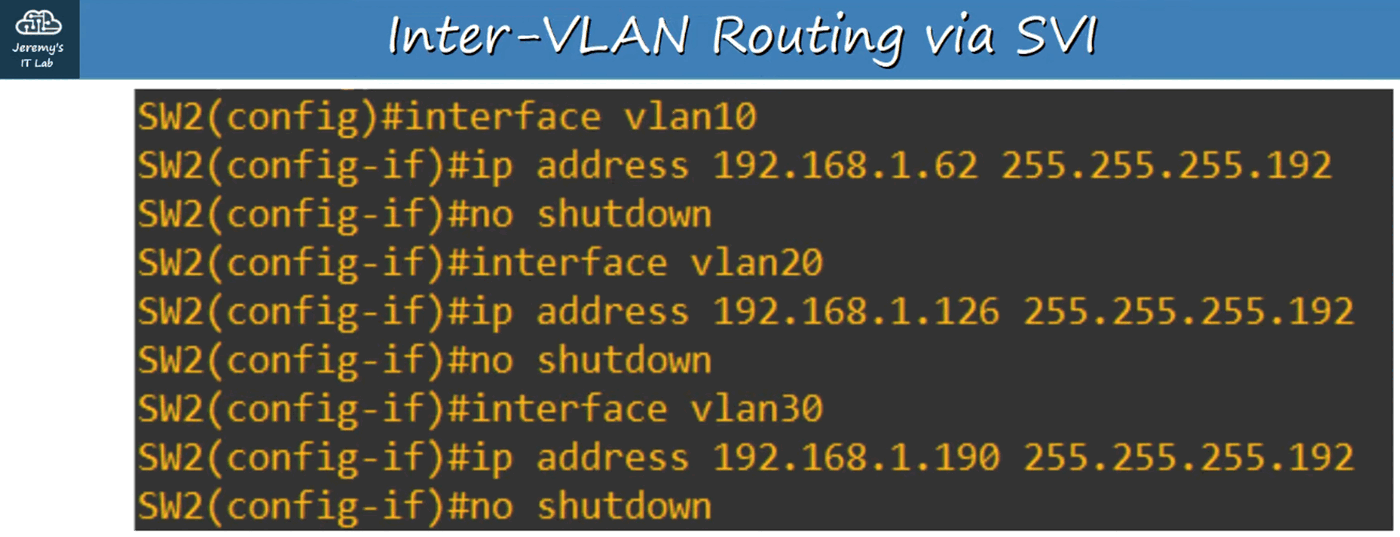
\includegraphics[keepaspectratio,alt={image}]{images/19-vlan-part3/img-015.png}}
\end{figure}

SVIs are \textbf{shut down} by default, so remember to use ``no
shutdown''

\begin{figure}
\centering
\pandocbounded{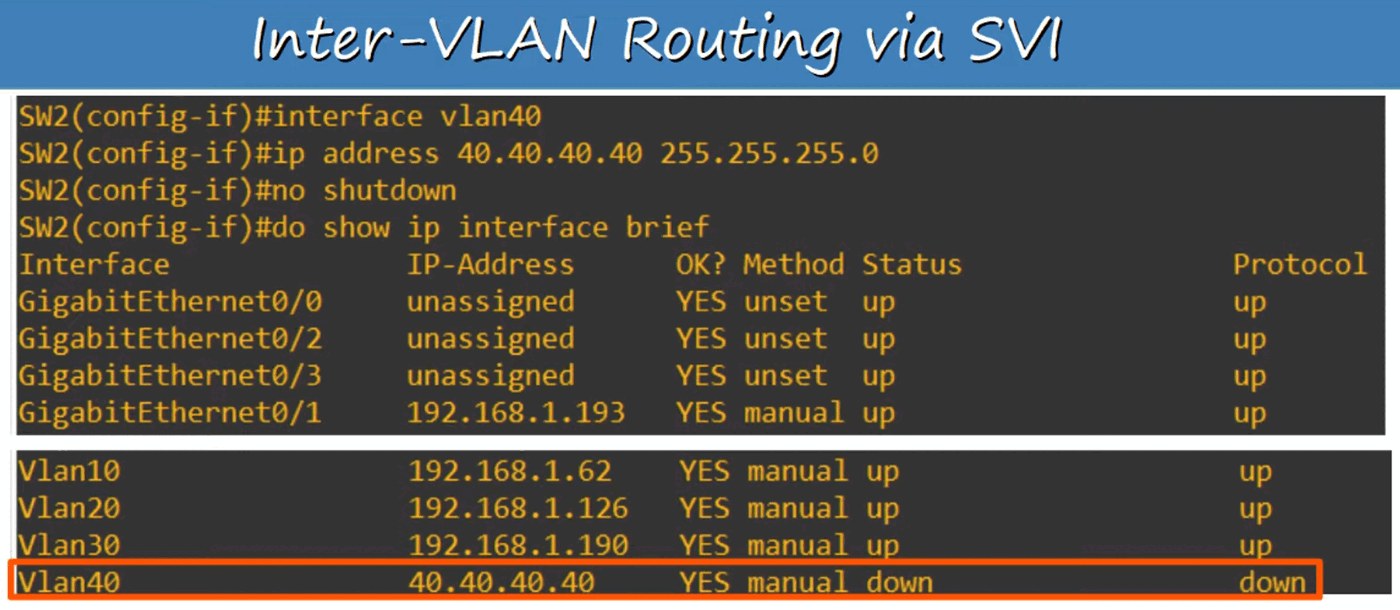
\includegraphics[keepaspectratio,alt={image}]{images/19-vlan-part3/img-016.png}}
\end{figure}

Creating an unknown SVI (VLAN 40) and the Status/Protocol is
``down/down''

What are the conditions for a SVI to be ``up/up'' ?

\begin{itemize}
\tightlist
\item
  The VLAN must exist on the SWITCH
\item
  The SWITCH must have at least ONE access port in the VLAN in an
  ``up/up'' state AND/OR one TRUNK port that allows the VLAN that is in
  an ``up/up'' state
\item
  The VLAN must not be shutdown (you can use the ``shutdown'' command to
  disable a VLAN)
\item
  The SVI must not be shutdown (SVIs are disabled, by default)
\end{itemize}

\begin{figure}
\centering
\pandocbounded{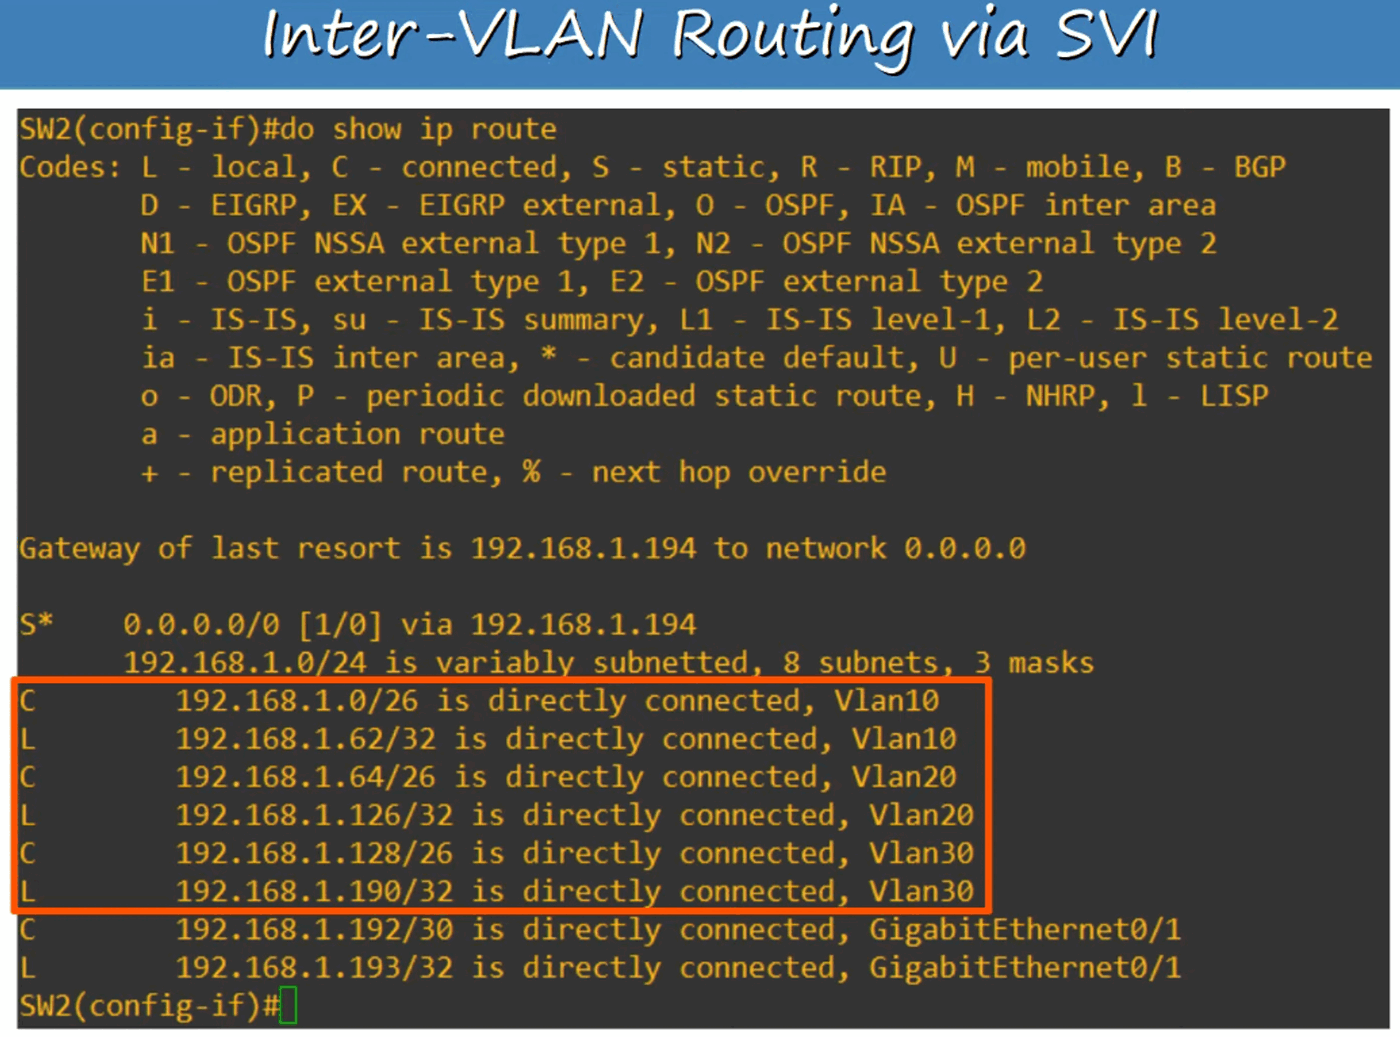
\includegraphics[keepaspectratio,alt={image}]{images/19-vlan-part3/img-017.png}}
\end{figure}

The VLAN trunk has been successfully replaced by an Layer 3 SWITCH SVI.

All hosts should be able to connect with each other (tested with
``ping'') as well as reach the external internet (via the Cloud symbol
attached to R1)

\chapter{DTP and VTP}\label{dtp-and-vtp}

DTP (Dynamic Trunking Protocol)

\begin{itemize}
\tightlist
\item
  Protocol that allows SWITCHES to negotiate the status of their
  SWITCHPORTS, without manual configuration, to be:

  \begin{itemize}
  \tightlist
  \item
    ACCESS PORTS
  \item
    TRUNK PORTS
  \end{itemize}
\item
  DTP is ENABLED by default on all Cisco SWITCH interfaces
\end{itemize}

We've been manually configuring SWITCHPORTS using :

\begin{itemize}
\tightlist
\item
  ``switchport mode access''
\item
  ``switchport mode trunk''
\end{itemize}

\begin{tipbox}

`show interfaces switchport' will show you a switchport's settings.

\end{tipbox}

For security purposes, \textbf{manual configuration} is recommended. DTP
should be disabled on ALL SWITCHPORTS

\begin{figure}
\centering
\pandocbounded{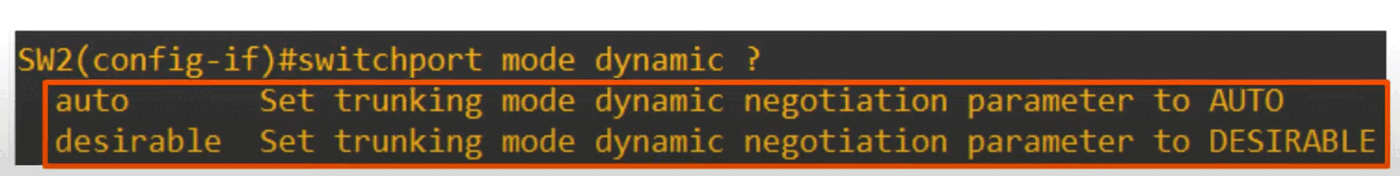
\includegraphics[keepaspectratio,alt={image}]{images/20-dtp-vtp/img-001.png}}
\end{figure}

\section{Dynamic Desirable}\label{dynamic-desirable}

\begin{itemize}
\tightlist
\item
  This MODE will actively try to form a TRUNK with other Cisco SWITCHES.
\item
  Will form a TRUNK if connected to another SWITCHPORT in the following
  modes:

  \begin{itemize}
  \tightlist
  \item
    ``switchport mode trunk''
  \item
    ``switchport mode dynamic desirable''
  \item
    ``switchport mode dynamic auto''
  \end{itemize}
\end{itemize}

HOWEVER \ldots{} if the other interface is set to ``static access''
(ACCESS mode), it will NOT form a TRUNK, it will be an ACCESS PORT

\section{Dynamic Auto}\label{dynamic-auto}

\begin{itemize}
\tightlist
\item
  This MODE will NOT actively try to form a TRUNK with other Cisco
  SWITCHES
\item
  Will form a TRUNK if connected SWTICH is actively trying to form a
  TRUNK.
\item
  It will form a TRUNK with a SWITCHPORT in the following modes:

  \begin{itemize}
  \tightlist
  \item
    ``switchport mode trunk''
  \item
    ``switchport mode dynamic desirable''
  \end{itemize}
\end{itemize}

TRUNK to ACCESS connection will operate in a \textbf{Mismatched Mode}.

This configuration does NOT work and SHOULD result in an error. Traffic
will NOT work.

\section{Table Showing the Different Modes and Compatibility in Forming
a
Trunk}\label{table-showing-the-different-modes-and-compatibility-in-forming-a-trunk}

\begin{figure}
\centering
\pandocbounded{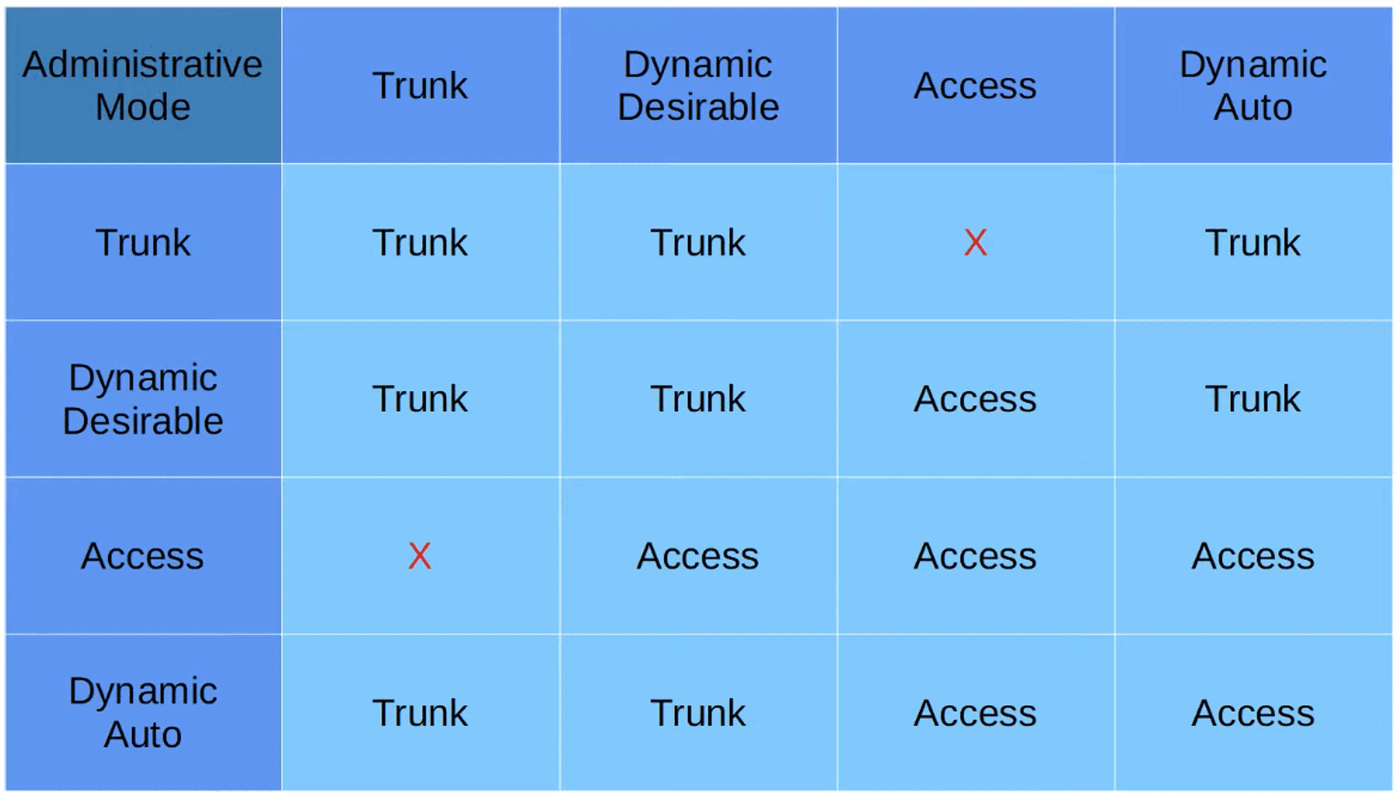
\includegraphics[keepaspectratio,alt={image}]{images/20-dtp-vtp/img-002.png}}
\end{figure}

DTP will NOT form a TRUNK with:

a ROUTER

a PC

etcetera \ldots{}

The SWITCHPORT will be in ACCESS Mode only!

\section{Old Switches}\label{old-switches}

\begin{itemize}
\tightlist
\item
  ``switchport mode dynamic desirable'' = Default administrative mode.
\end{itemize}

\section{Newer Switches}\label{newer-switches}

\begin{itemize}
\tightlist
\item
  ``switchport mode dynamic auto'' = Default administrative mode.
\end{itemize}

\section{How to Disable DTP Negotiation on an
Interface}\label{how-to-disable-dtp-negotiation-on-an-interface}

\begin{itemize}
\tightlist
\item
  ``switchport nonegotiate''
\item
  ``switchport mode access''
\end{itemize}

It is a security recommendation to disable DTP on all SWITCHPORTS and
manually configure them as ACCESS or TRUNK ports.

\section{Encapsulation}\label{encapsulation}

SWITCHES that support both:

\begin{itemize}
\tightlist
\item
  802.1Q
\item
  ISL
\end{itemize}

TRUNK encapsulation can use DTP to negotiate the encapsulation they will
use.

\begin{itemize}
\tightlist
\item
  Negotiation is Enabled by default
\end{itemize}

\begin{tipbox}

`switchport trunk encapsulation negotiate'

\end{tipbox}

\begin{itemize}
\tightlist
\item
  ISL is favored over 802.1Q

  \begin{itemize}
  \tightlist
  \item
    If BOTH SWITCHES support ISL, ISL will be selected.
  \end{itemize}
\item
  DTP frames are sent in:

  \begin{itemize}
  \tightlist
  \item
    VLAN1 when using ISL
  \item
    Native VLAN when using 802.1Q (the default native VLAN is VLAN1,
    however)
  \end{itemize}
\end{itemize}

VTP (VLAN Trunking Protocol)

In Privileged EXEC mode:

\begin{tipbox}

\#show vtp status

\end{tipbox}

\begin{itemize}
\item
  Protocol for configuring VLANs on a Central SWITCH

  \begin{itemize}
  \tightlist
  \item
    A SERVER that other SWITCHES synch. to (auto configuring by
    connection)
  \end{itemize}
\item
  Other switches (VTP CLIENTS) will synchronize their VLAN database to
  the SERVER
\item
  Designed for large networks with many VLANs (reduces manual
  configuration)
\item
  RARELY used. Recommended you DO NOT USE it
\item
  There are THREE VTP Versions :

  \begin{itemize}
  \tightlist
  \item
    v1

    \begin{itemize}
    \tightlist
    \item
      Does NOT supports Extended VLAN Range 1006-4094
    \end{itemize}
  \item
    v2

    \begin{itemize}
    \tightlist
    \item
      Does NOT supports Extended VLAN Range 1006-4094
    \item
      Supports Token Ring VLANs ; otherwise similar to V1
    \end{itemize}
  \item
    v3

    \begin{itemize}
    \tightlist
    \item
      Supports Extended VLAN Range 1006-4094
    \item
      CLIENTS store VLAN dBase in NVRAM
    \end{itemize}
  \end{itemize}
\item
  There are \textbf{THREE VTP modes}:

  \begin{itemize}
  \tightlist
  \item
    SERVER
  \item
    CLIENT
  \item
    TRANSPARENT
  \end{itemize}
\item
  Cisco SWITCHES operate in VTP SERVER mode, by default
\end{itemize}

\begin{figure}
\centering
\pandocbounded{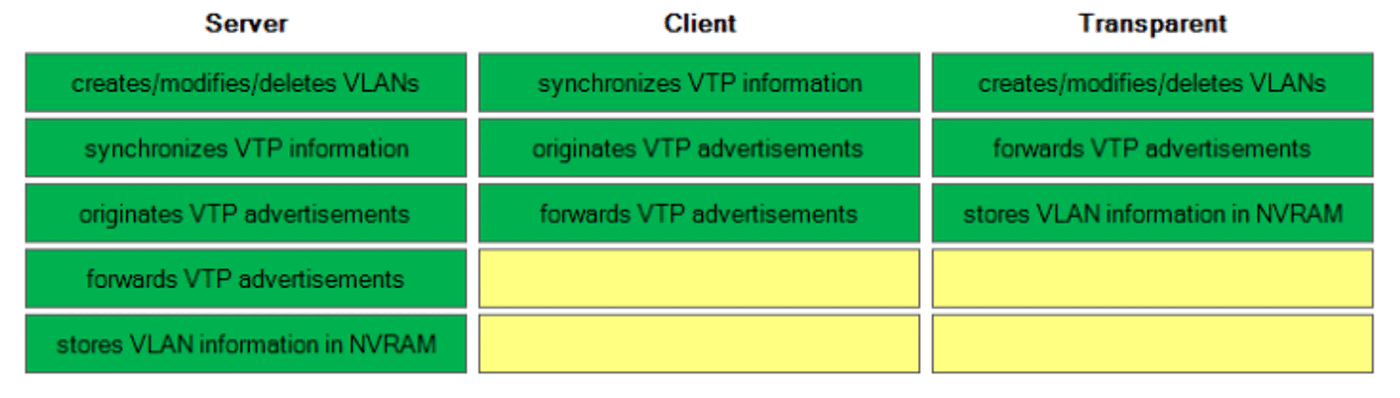
\includegraphics[keepaspectratio,alt={image}]{images/20-dtp-vtp/img-003.png}}
\end{figure}

\section{VTP Servers}\label{vtp-servers}

\begin{itemize}
\tightlist
\item
  Can ADD / MODIFY / DELETE VLANs
\item
  Store the VLAN dBase in NVRAM
\item
  Increase Revision Number every time VLAN is Added / Modified / Deleted
\item
  Advertises \textbf{Latest Version} of VLAN dBase on TRUNK interfaces.
\item
  VTP CLIENTS synchronize their VLAN dBase to it
\item
  \textbf{VTP SERVERS also function as VTP CLIENTS}

  \begin{itemize}
  \tightlist
  \item
    \textbf{THEREFORE, a VTP SERVER will synchronize to another VTP
    SERVER with a higher Revision Number}
  \end{itemize}
\end{itemize}

\begin{warnbox}

One danger of VTP: Connecting an old SWITCH with higher Revision Number
to network (and if the VTP Domain Name matches), all SWITCHES in Domain
will synchronize their VLAN dBase to SWITCH

\end{warnbox}

\section{VTP Clients}\label{vtp-clients}

\begin{tipbox}

(config)\# vtp mode client

\end{tipbox}

\begin{itemize}
\tightlist
\item
  Cannot Add / Modify / Delete VLANs
\item
  Does NOT store the VLAN database in NVRAM

  \begin{itemize}
  \tightlist
  \item
    \textbf{VTP v3 CLIENTS DO}
  \end{itemize}
\item
  Will synchronize their VLAN dBase to the SERVER with the highest
  version number in their VTP Domain
\item
  Advertise their VLAN dBase and forward VTP Advertisements to other
  CLIENTS over TRUNK Ports
\end{itemize}

\section{VTP Transparent Mode}\label{vtp-transparent-mode}

\begin{tipbox}

(config)\# vtp mode transparent

\end{tipbox}

\begin{itemize}
\tightlist
\item
  Does NOT participate in VTP Domain (does NOT sync VLAN database)
\item
  Maintains own VLAN dBase in NVRAM.
\item
  Can Add / Modify / Delete VLANs
\item
  Won't Advertise to other SWITCHES
\item
  Will forward VTP advertisements to SWITCHES in the same Domain as it.
\end{itemize}

\section{VTP Domains}\label{vtp-domains}

If a SWITCH with no VTP Domain (Domain NULL) receives a VTP
advertisement with a VTP Domain name, it will automatically join that
VTP Domain

If a SWITCH receives a VTP advertisement in the same VTP domain with a
higher revision number, it will update it's VLAN database to match

\section{Revision Numbers}\label{revision-numbers}

There are TWO ways to RESET a REVISION NUMBER to 0:

\begin{itemize}
\tightlist
\item
  Change VTP Domain to an unused Domain
\item
  Change VTP mode to TRANSPARENT
\end{itemize}

\section{VTP Version Number}\label{vtp-version-number}

\begin{tipbox}

(config)\#vtp version

\end{tipbox}

Changing the Version \# will force sync/update all connected SWITCHES to
the latest Version \#

\chapter{Spanning Tree Protocol: Part
1}\label{spanning-tree-protocol-part-1}

\section{Redundancy in Networks}\label{redundancy-in-networks}

\begin{itemize}
\tightlist
\item
  Essential in network design
\item
  Modern networks are expected to run 24/7/265; even a short downtime
  can be disastrous for business.
\item
  If one network component fails, you must ensure that other components
  will take over with little or no downtime.
\item
  As much as possible, you must implement REDUNDANCY at every possible
  point in the network
\end{itemize}

\section{An Example of a Poorly Designed
Network}\label{an-example-of-a-poorly-designed-network}

\begin{figure}
\centering
\pandocbounded{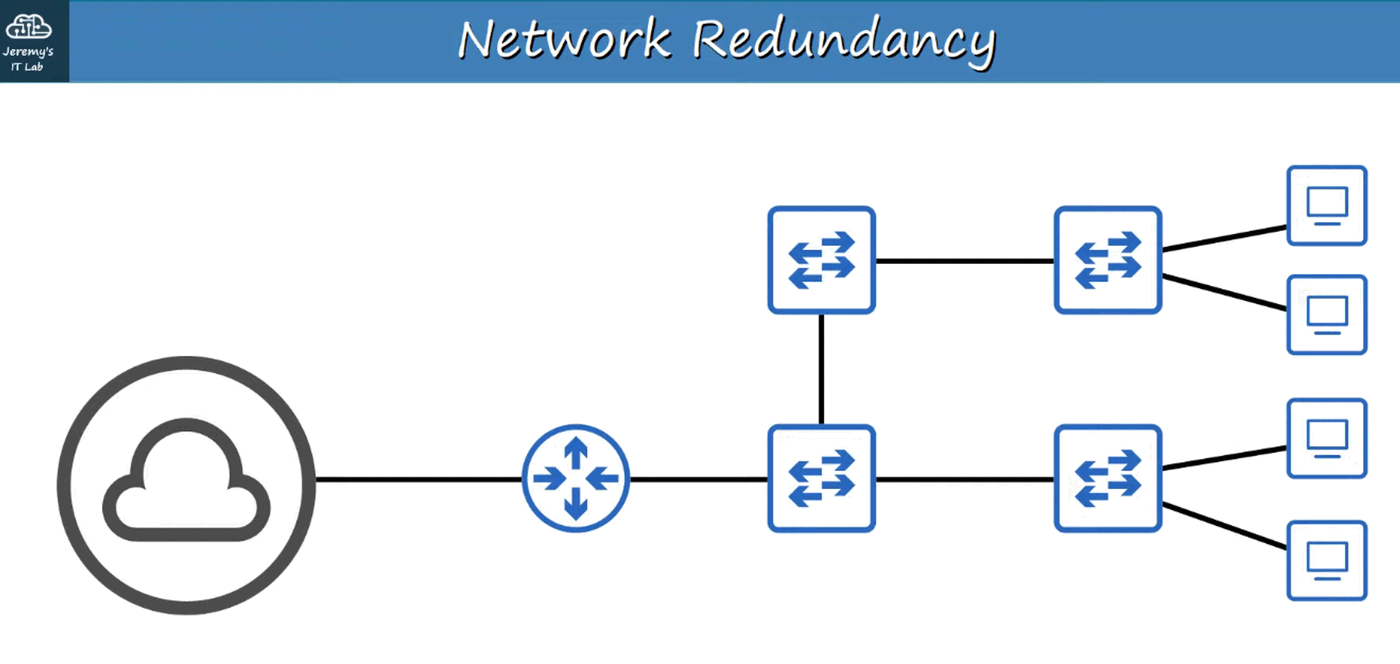
\includegraphics[keepaspectratio,alt={image}]{images/21-spanning-tree-protocol-part1/img-001.png}}
\end{figure}

NOTE the many single-point failures that could occur (single
connections)

\section{A Better Network Design}\label{a-better-network-design}

\begin{figure}
\centering
\pandocbounded{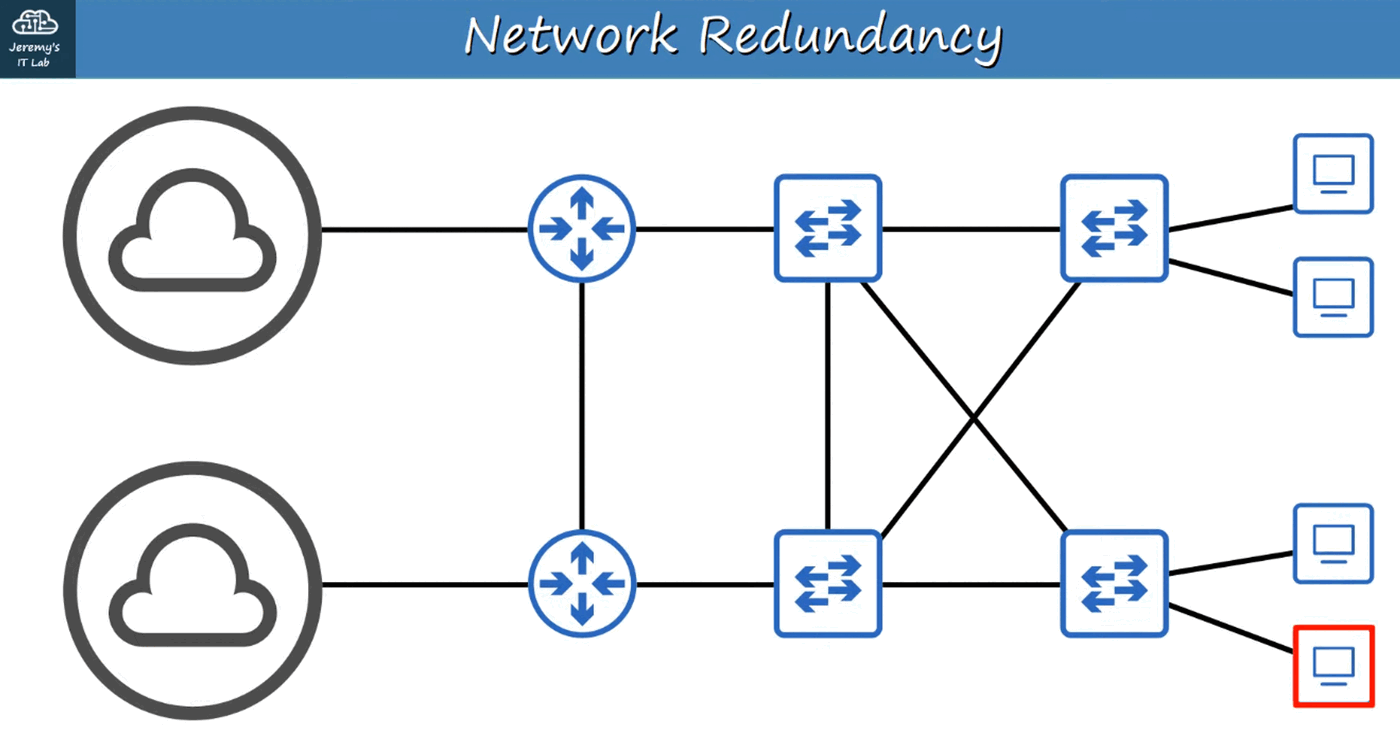
\includegraphics[keepaspectratio,alt={image}]{images/21-spanning-tree-protocol-part1/img-002.png}}
\end{figure}

\section{Unfortunately}\label{unfortunately}

\begin{itemize}
\tightlist
\item
  Most PCS only have a single network interface card (NIC), so they can
  only be plugged into a single SWITCH. However, important SERVERS
  typically have multiple NICs, so they can be plugged into multiple
  SWITCHES for redundancy!
\end{itemize}

So HOW can all this redundancy be a BAD thing?

\section{Broadcast Storms}\label{broadcast-storms}

\begin{figure}
\centering
\pandocbounded{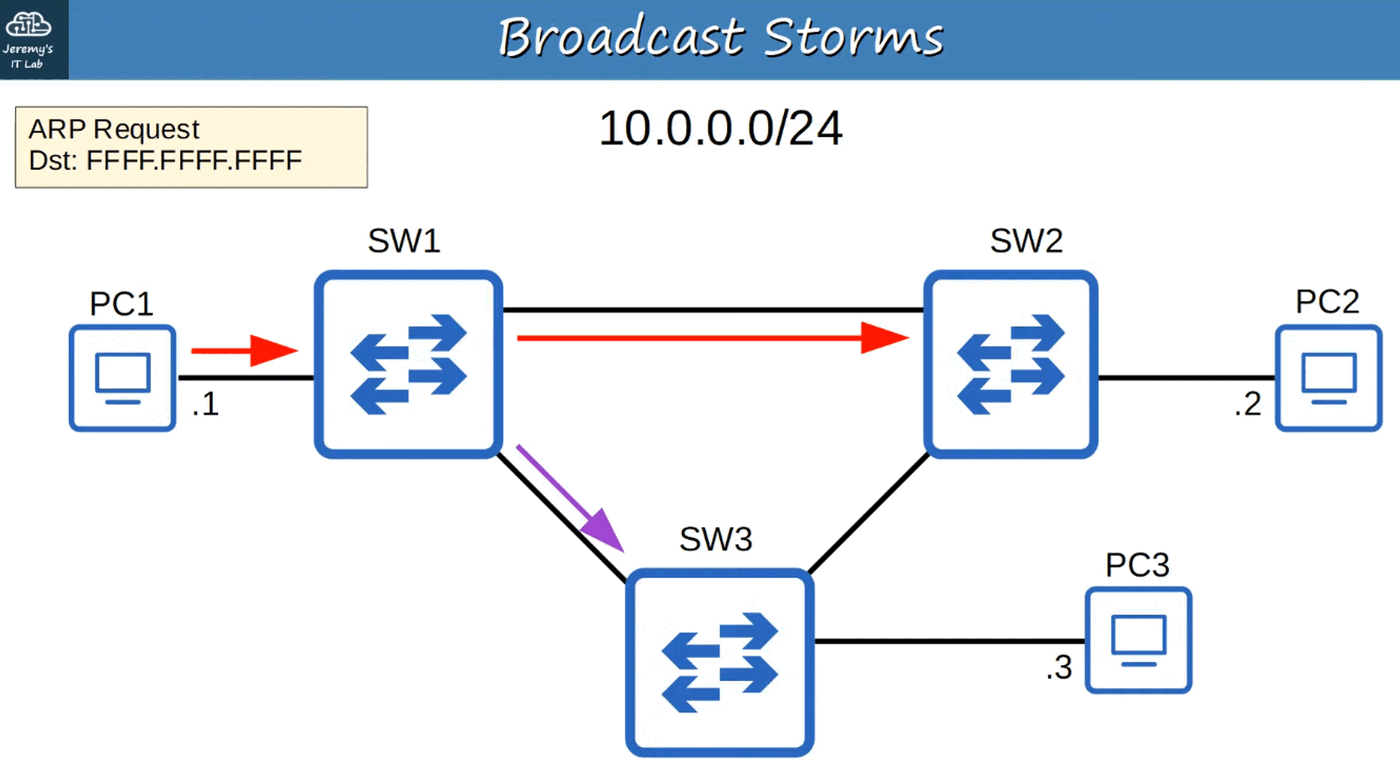
\includegraphics[keepaspectratio,alt={image}]{images/21-spanning-tree-protocol-part1/img-003.png}}
\end{figure}

\begin{figure}
\centering
\pandocbounded{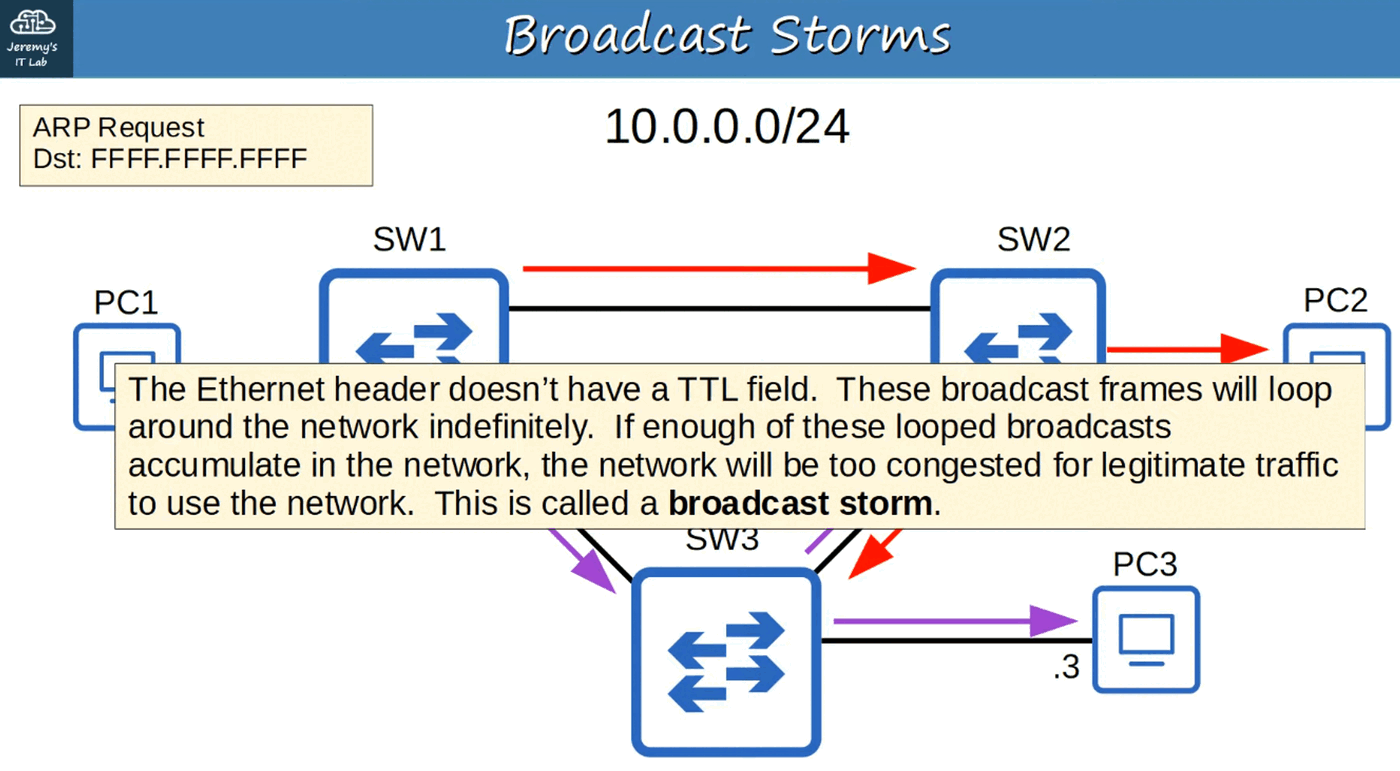
\includegraphics[keepaspectratio,alt={image}]{images/21-spanning-tree-protocol-part1/img-004.png}}
\end{figure}

\begin{figure}
\centering
\pandocbounded{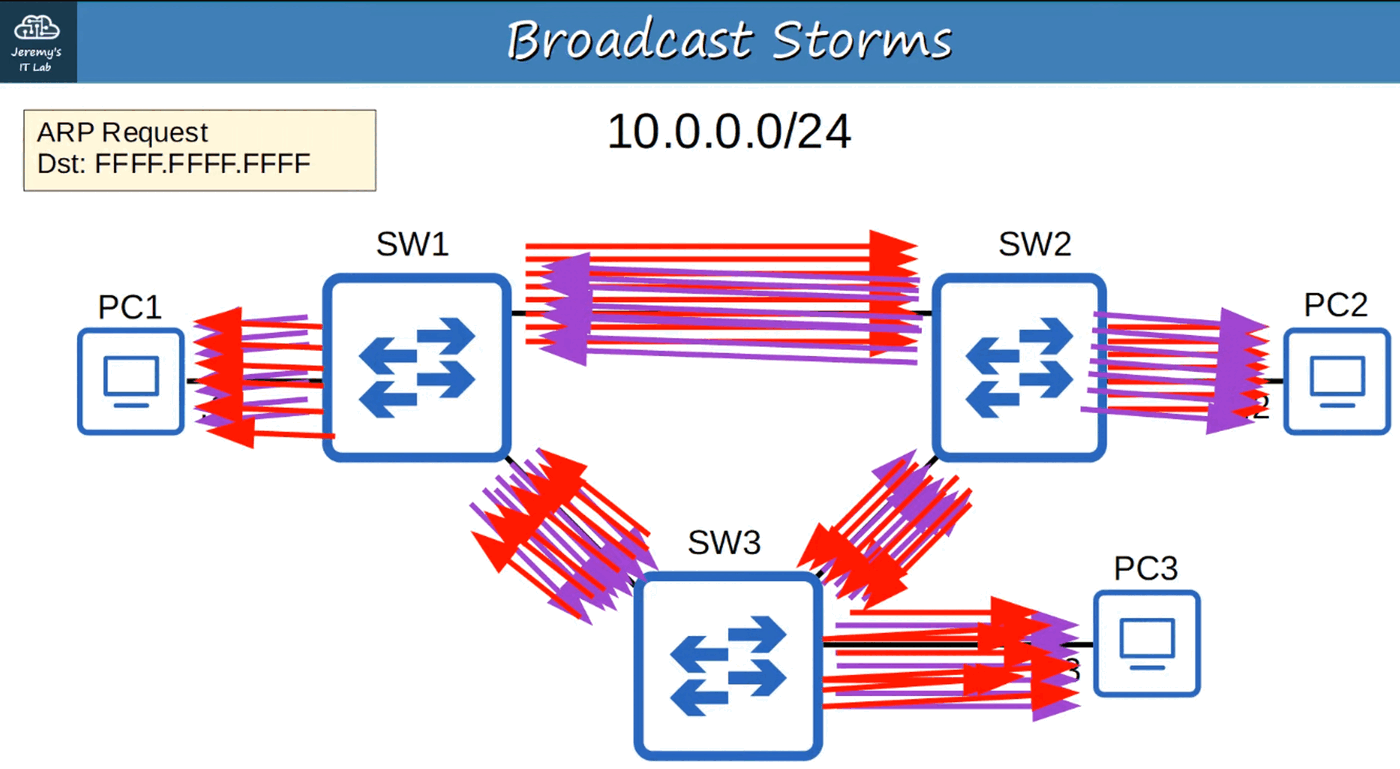
\includegraphics[keepaspectratio,alt={image}]{images/21-spanning-tree-protocol-part1/img-005.png}}
\end{figure}

FLOODED WITH ARP REQUESTS (Red = Clockwise Loops // Purple =
Counter-Clockwise Loops)

Network Congestion isn't the only problem.

Each time a FRAME arrives on a SWITCHPORT, the SWITCH uses the SOURCE
MAC ADDRESS field to ``learn'' the MAC ADDRESS and update it's MAC
ADDRESS TABLE.

When frames with the same SOURCE MAC ADDRESS repeatedly arrive on
different interfaces, the SWITCH is continuously updating the interface
in it's MAC ADDRESS TABLE.

This is called MAC ADDRESS FLAPPING

So how we design a network, with redundant paths, that doesn't result in
LAYER 2 LOOPS.

SPANNING TREE PROTOCOL is one solution

\section{STP (Spanning Tree Protocol) :
802.1D}\label{stp-spanning-tree-protocol-802.1d}

\begin{itemize}
\tightlist
\item
  ``Classic Spanning Tree Protocol'' is IEEE \textbf{802.1D}
\item
  SWITCHES from ALL vendors run STP by Default
\item
  STP prevents LAYER 2 loops by placing redundant PORTS in a BLOCKING
  state, essentially disabling the INTERFACE
\item
  These INTERFACES act as backups that can enter a FORWARDING state if
  an active (=currently forwarding) INTERFACE fails.
\item
  INTERFACES in a BLOCKING state only send or receive STP messages
  (called BPDUs = Bridge Protocol Data Units)
\end{itemize}

SPANNING TREE PROTOCOL still uses the term ``BRIDGE''. However, when use
the term ``BRIDGE'', we really mean ``SWITCH''. BRIDGES are not used in
modern networks.

\begin{figure}
\centering
\pandocbounded{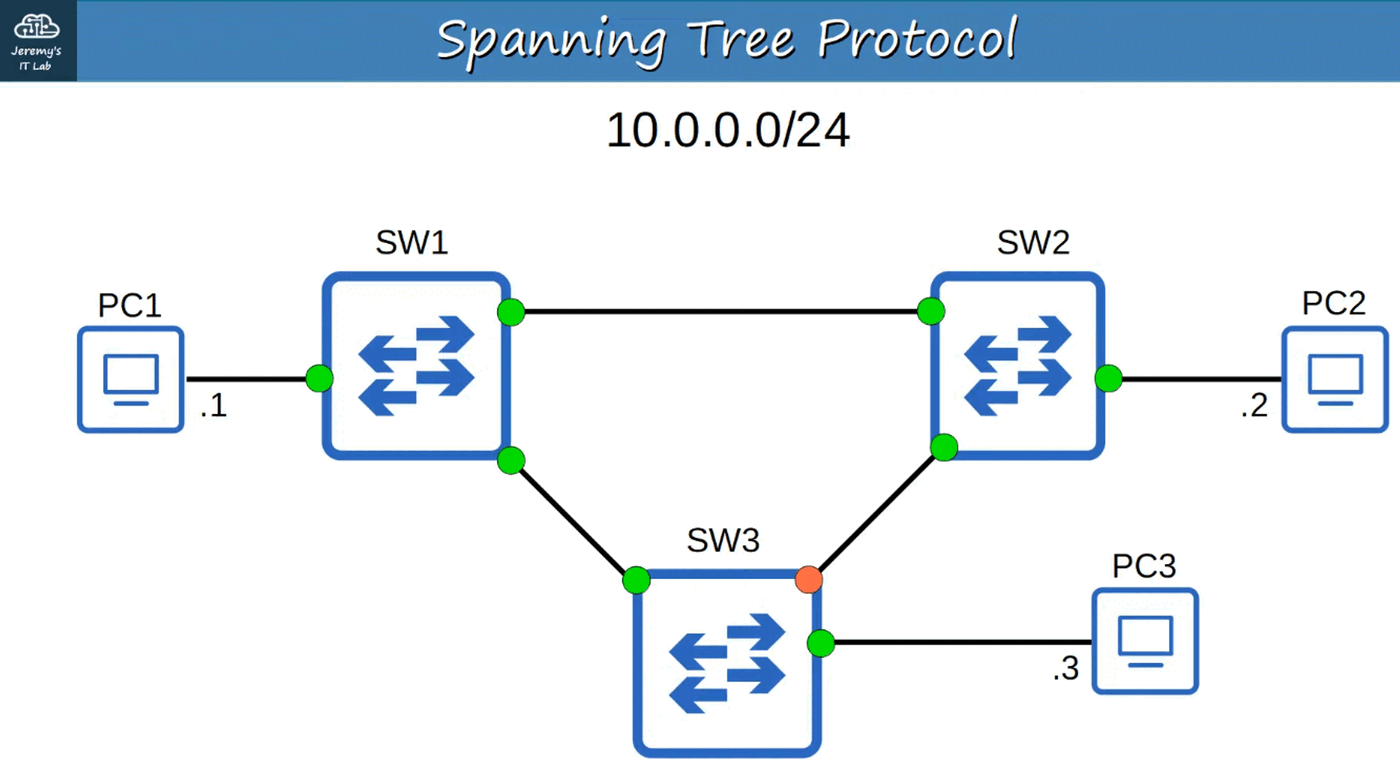
\includegraphics[keepaspectratio,alt={image}]{images/21-spanning-tree-protocol-part1/img-006.png}}
\end{figure}

ORANGE INTERFACE is ``BLOCKED'' causing a break in the loops

\begin{figure}
\centering
\pandocbounded{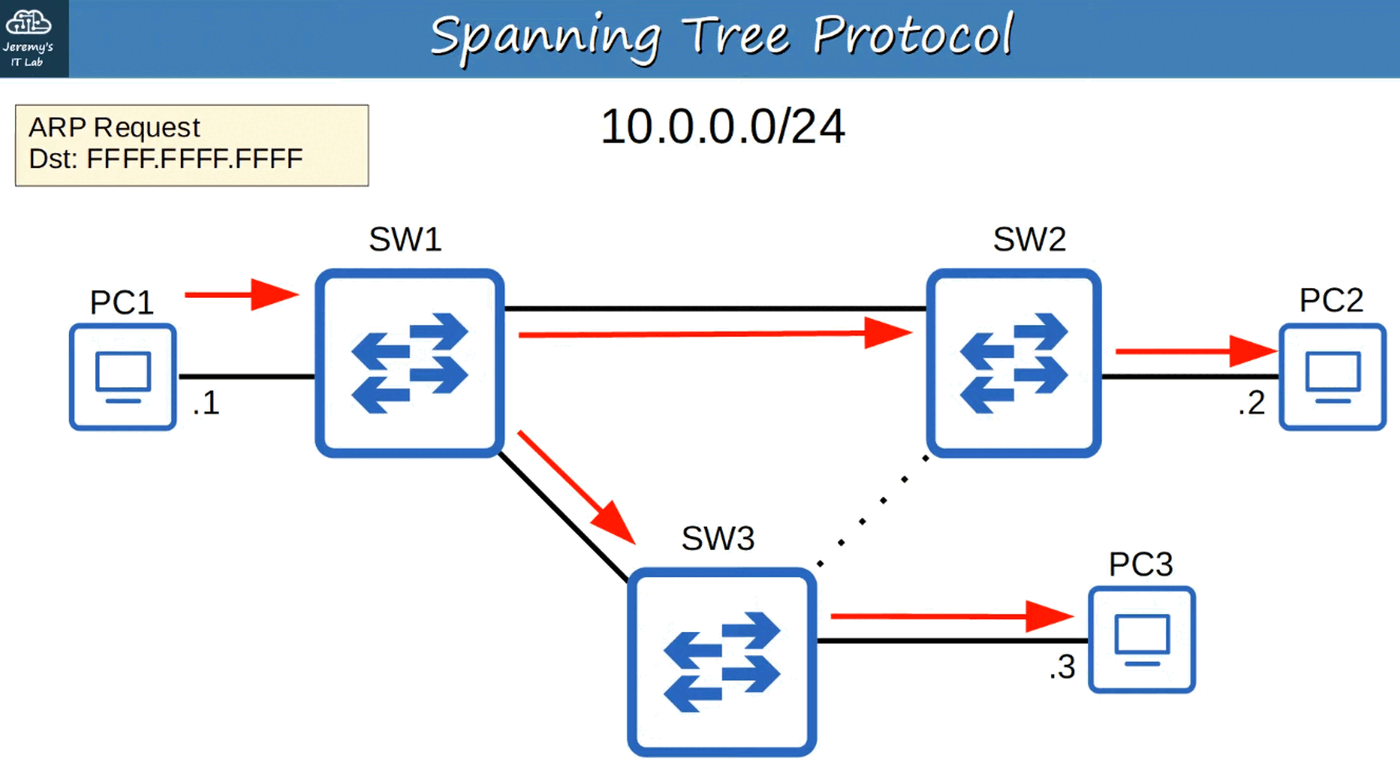
\includegraphics[keepaspectratio,alt={image}]{images/21-spanning-tree-protocol-part1/img-007.png}}
\end{figure}

If changes occur in the connections, the traffic will adjust the
topology.

\begin{itemize}
\tightlist
\item
  By selecting WHICH ports are FORWARDING and which ports are BLOCKING,
  STP creates a single path TO / FROM each point in the NETWORK. This
  prevents LAYER 2 Loops.
\item
  There is a set process that STP uses to determine which ports should
  be FORWARDING and which should be BLOCKING
\item
  STP-enabled SWITCHES send / receive ``Hello BPDUs'' out of all
  INTERFACES

  \begin{itemize}
  \tightlist
  \item
    The default timer is : ONCE every TWO seconds per INTERFACE!
  \end{itemize}
\item
  If a SWITCH receives a ``Hello BPDU'' on an INTERFACE, it knows that
  INTERFACE is connected to another SWITCH (ROUTERS, PCs, etc. do NOT
  use STP so do not send ``Hello BPDUs'')
\end{itemize}

WHAT ARE BPDUs USED FOR?

\begin{itemize}
\tightlist
\item
  SWITCHES use one field in the STP BPDU, the BRIDGE ID field, to elect
  a ROOT BRIDGE for the NETWORK
\item
  The SWITCH with the lowest BRIDGE ID becomes the ROOT BRIDGE
\item
  ALL PORTS on the ROOT BRIDGE are put in a FORWARDING state, and other
  SWITCHES in the topology must have a path to reach the ROOT BRIDGE
\end{itemize}

\begin{figure}
\centering
\pandocbounded{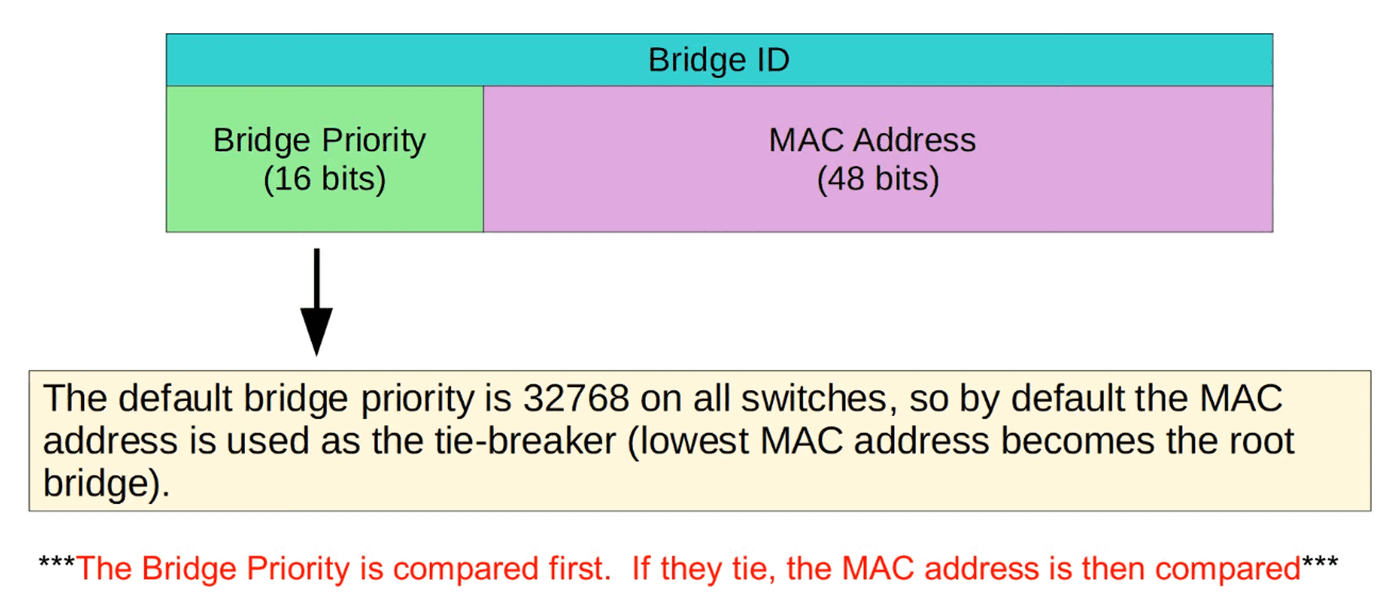
\includegraphics[keepaspectratio,alt={image}]{images/21-spanning-tree-protocol-part1/img-008.png}}
\end{figure}

\begin{figure}
\centering
\pandocbounded{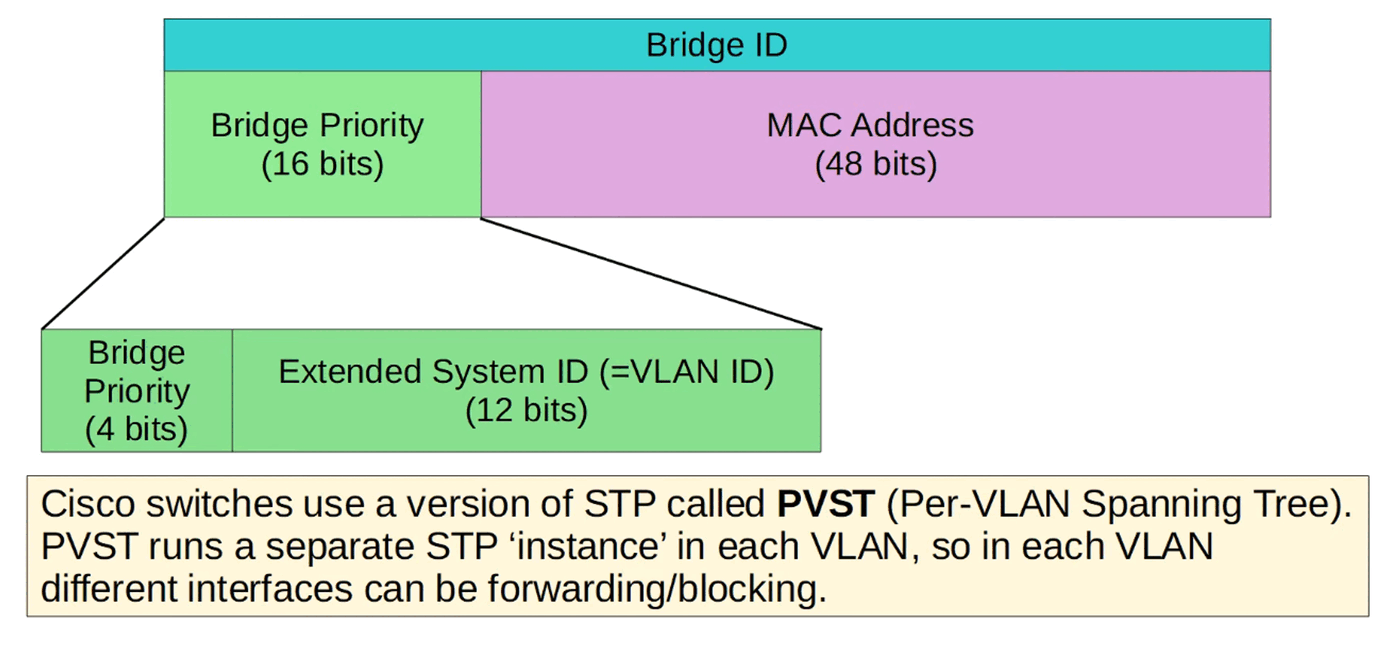
\includegraphics[keepaspectratio,alt={image}]{images/21-spanning-tree-protocol-part1/img-009.png}}
\end{figure}

\begin{figure}
\centering
\pandocbounded{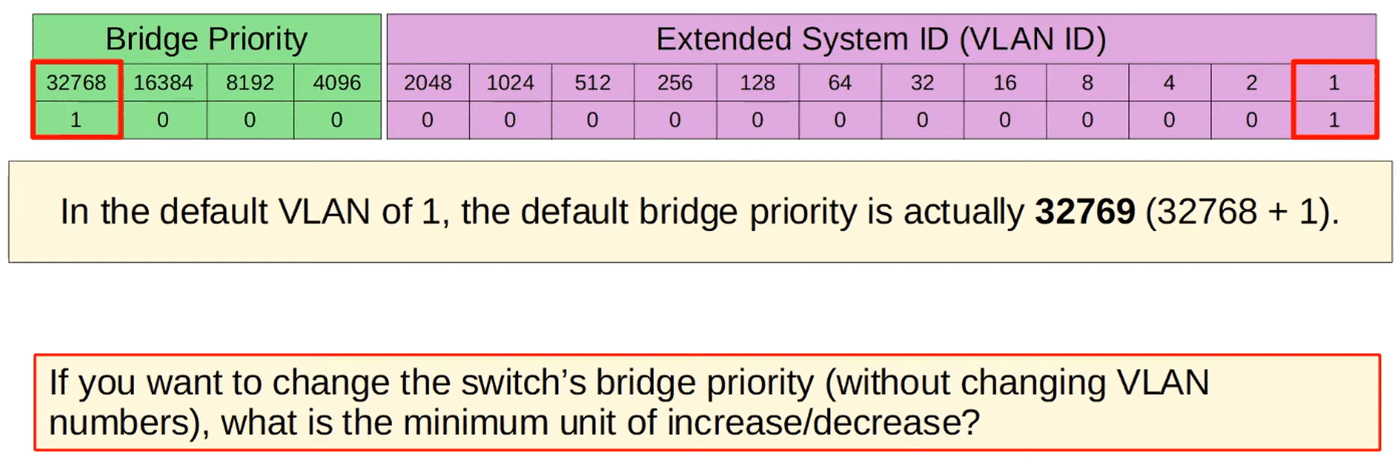
\includegraphics[keepaspectratio,alt={image}]{images/21-spanning-tree-protocol-part1/img-010.png}}
\end{figure}

To REDUCE the BRIDGE PRIORITY, we can only change it in units of 4096 !

\begin{figure}
\centering
\pandocbounded{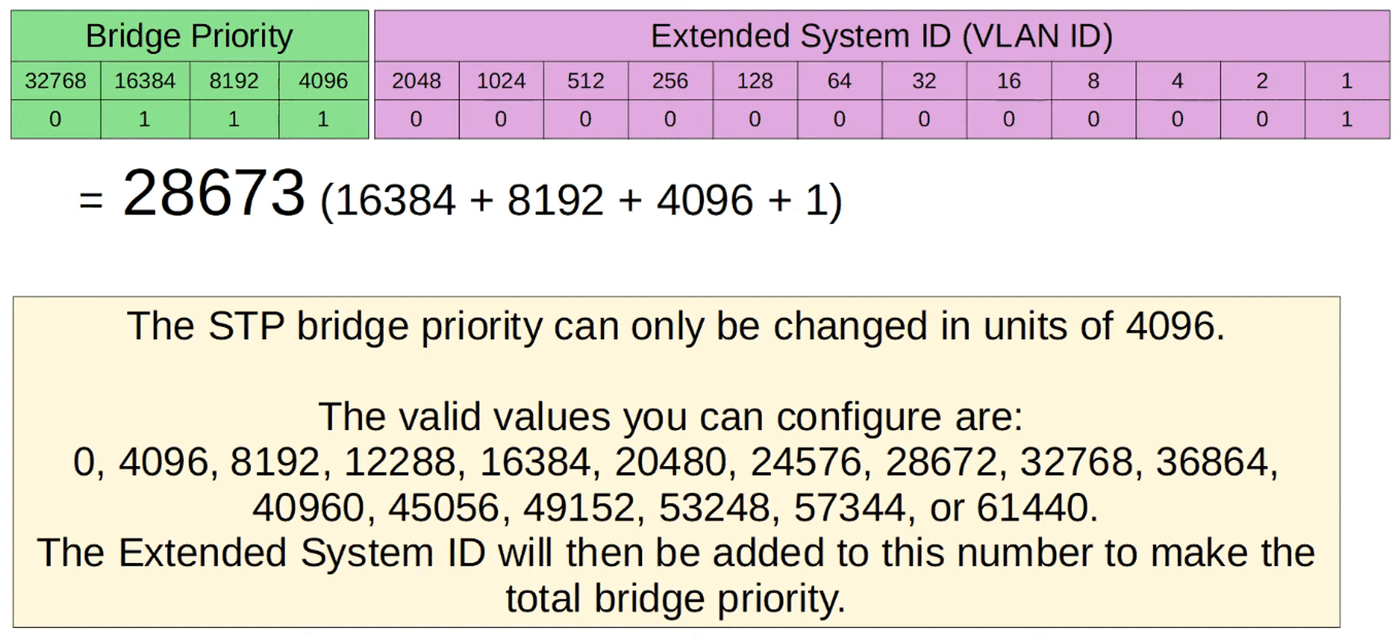
\includegraphics[keepaspectratio,alt={image}]{images/21-spanning-tree-protocol-part1/img-011.png}}
\end{figure}

In THIS TOPOLOGY, SW1 becomes the ROOT BRIDGE due to it's MAC ADDRESS
being LOWEST

(Hex ``A'' = 10)

\begin{figure}
\centering
\pandocbounded{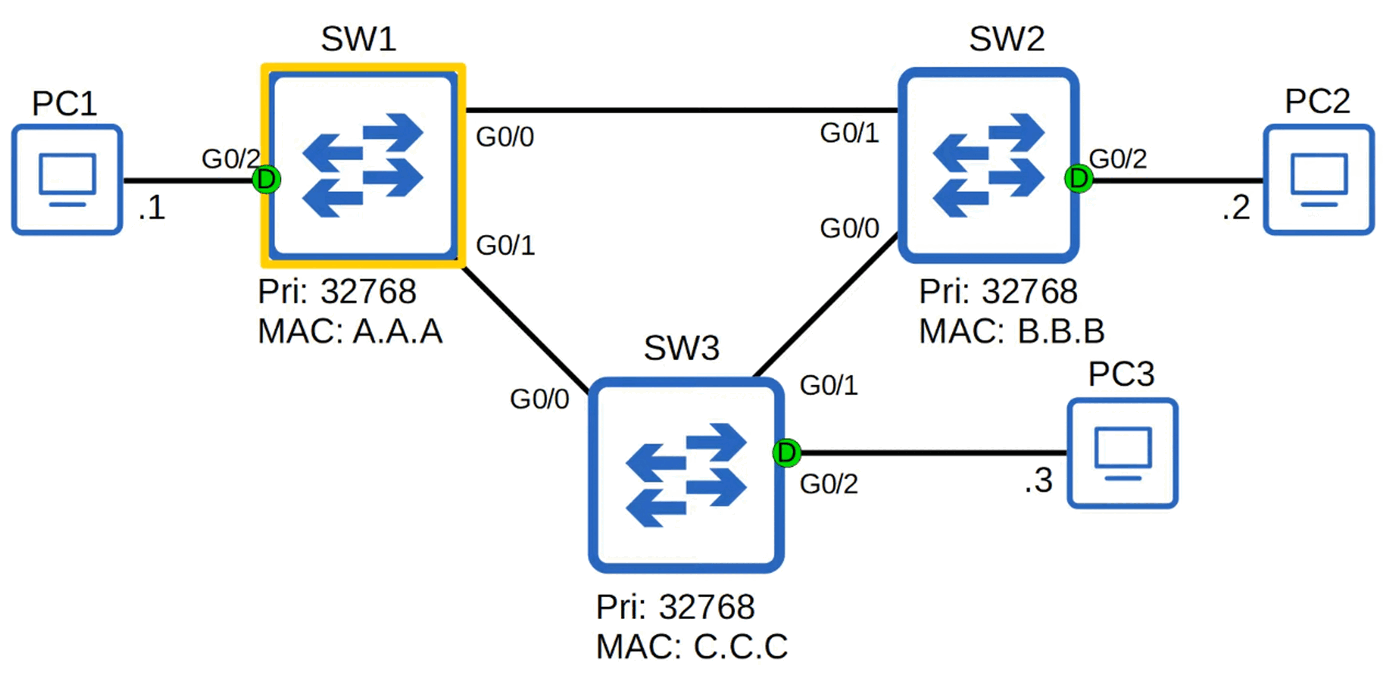
\includegraphics[keepaspectratio,alt={image}]{images/21-spanning-tree-protocol-part1/img-012.png}}
\end{figure}

ALL INTERFACES on the ROOT BRIDGE are DESIGNATED PORTS.

DESIGNATED PORTS ARE IN A FORWARDING STATE!

\section{Root Bridge}\label{root-bridge}

\begin{itemize}
\tightlist
\item
  When a SWITCH is powered on, it assumes it is the ROOT BRIDGE
\item
  It will only give up its position if it receives a ``SUPERIOR'' BPDU
  (lower BRIDGE ID)
\item
  Once the topology has converged and all SWITCHES agree on the ROOT
  BRIDGE, only the ROOT BRIDGE sends BPDUs
\item
  Other SWITCHES in the network will forward these BPDUs, but will not
  generate their own original BPDUs
\end{itemize}

\section{Spanning Tree Protocol
Steps}\label{spanning-tree-protocol-steps}

\begin{enumerate}
\def\labelenumi{\arabic{enumi})}
\tightlist
\item
  One SWITCH is elected as ROOT BRIDGE. All PORTS on the ROOT BRIDGE are
  DESIGNATED PORTS (FORWARDING STATE)
\end{enumerate}

\begin{itemize}
\tightlist
\item
  ROOT BRIDGE selection order:

  \begin{itemize}
  \tightlist
  \item
    \begin{enumerate}
    \def\labelenumi{\arabic{enumi})}
    \tightlist
    \item
      Lowest BRIDGE ID
    \end{enumerate}
  \item
    2) Lowest MAC Address (in case of Bridge ID tie)
  \end{itemize}
\end{itemize}

\begin{enumerate}
\def\labelenumi{\arabic{enumi})}
\setcounter{enumi}{1}
\tightlist
\item
  Each remaining SWITCH will select ONE of its INTERFACES to be it's
  ROOT PORT (FORWARDING STATE). PORTS across from the ROOT PORT are
  always DESIGNATED PORTS.
\end{enumerate}

\begin{itemize}
\tightlist
\item
  ROOT PORT selection order:

  \begin{itemize}
  \tightlist
  \item
    \begin{enumerate}
    \def\labelenumi{\arabic{enumi})}
    \tightlist
    \item
      LOWEST ROOT COST (see STP COST CHART)
    \end{enumerate}
  \item
    2) LOWEST NEIGHBOUR BRIDGE ID
  \item
    3) LOWEST NEIGHBOUR PORT ID
  \end{itemize}
\end{itemize}

\begin{enumerate}
\def\labelenumi{\arabic{enumi})}
\setcounter{enumi}{2}
\tightlist
\item
  Each remaining COLLISION DOMAIN will select ONE INTERFACE to be a
  DESIGNATION PORT (FORWARDING STATE). The other PORT in the COLLISION
  DOMAIN will NON-DESIGNATED (BLOCKING)
\end{enumerate}

\begin{itemize}
\tightlist
\item
  DESIGNATED PORT SELECTION:

  \begin{itemize}
  \tightlist
  \item
    \begin{enumerate}
    \def\labelenumi{\arabic{enumi})}
    \tightlist
    \item
      INTERFACE on SWITCH with LOWEST ROOT COST
    \end{enumerate}
  \item
    2) INTERFACE on SWITCH with LOWEST BRIDGE ID
  \end{itemize}
\end{itemize}

\section{STP Cost Chart}\label{stp-cost-chart}

Only OUTGOING INTERFACES toward the ROOT BRIDGE have a STP COST; not
RECEIVING INTERFACES. Add up all the OUTGOING PORT costs until you reach
the ROOT BRIDGE

\begin{figure}
\centering
\pandocbounded{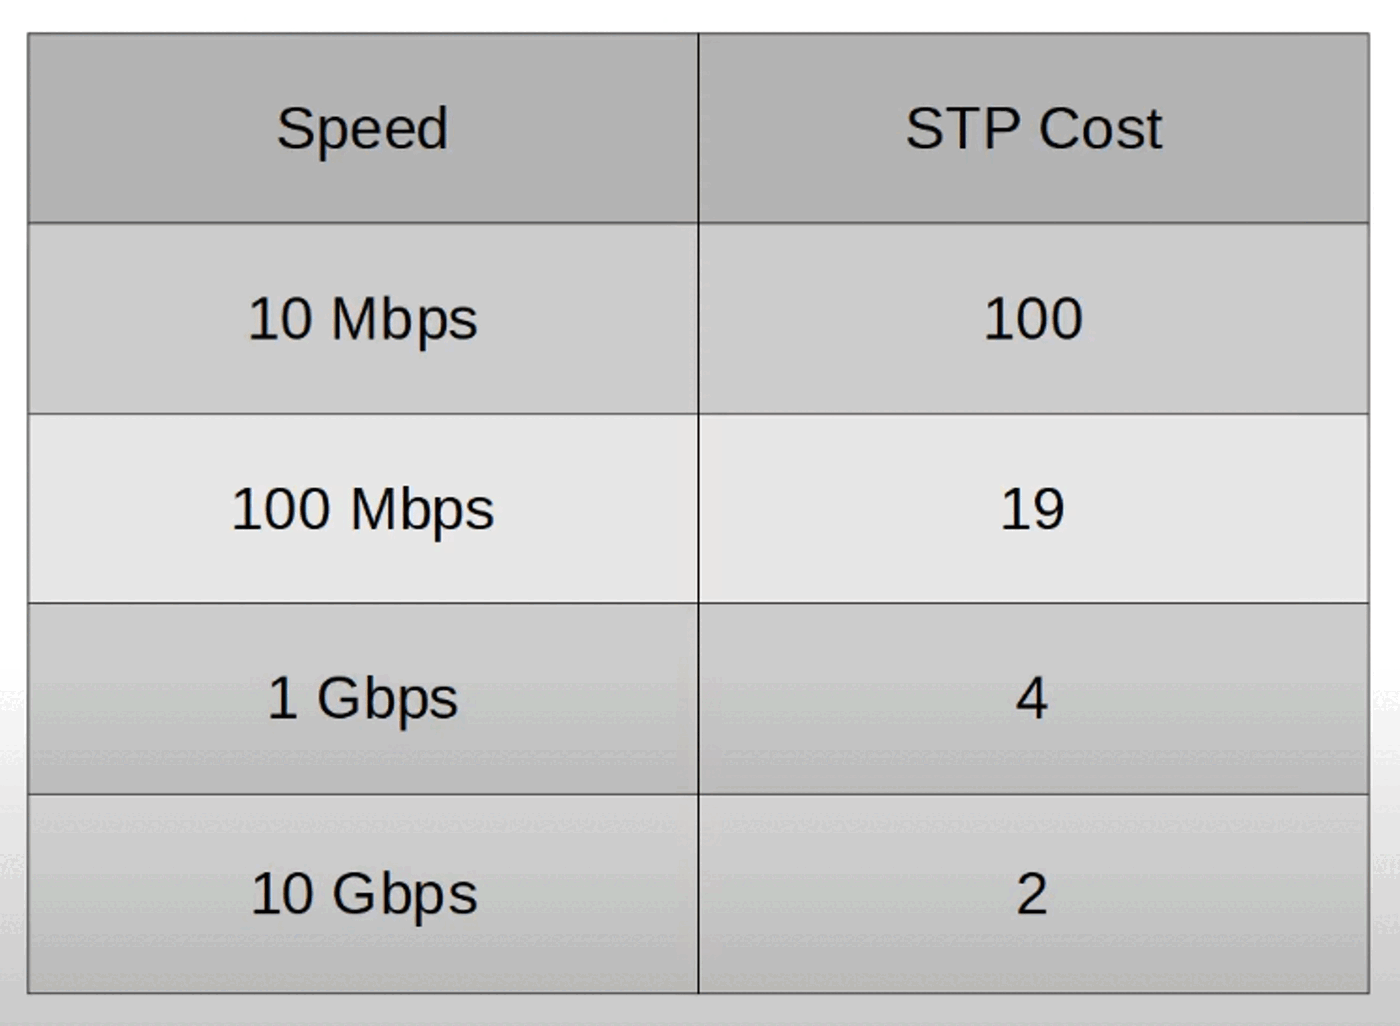
\includegraphics[keepaspectratio,alt={image}]{images/21-spanning-tree-protocol-part1/img-013.png}}
\end{figure}

SW1 is the ROOT BRIDGE so has a STP COST of 0 on ALL INTERFACES

\begin{figure}
\centering
\pandocbounded{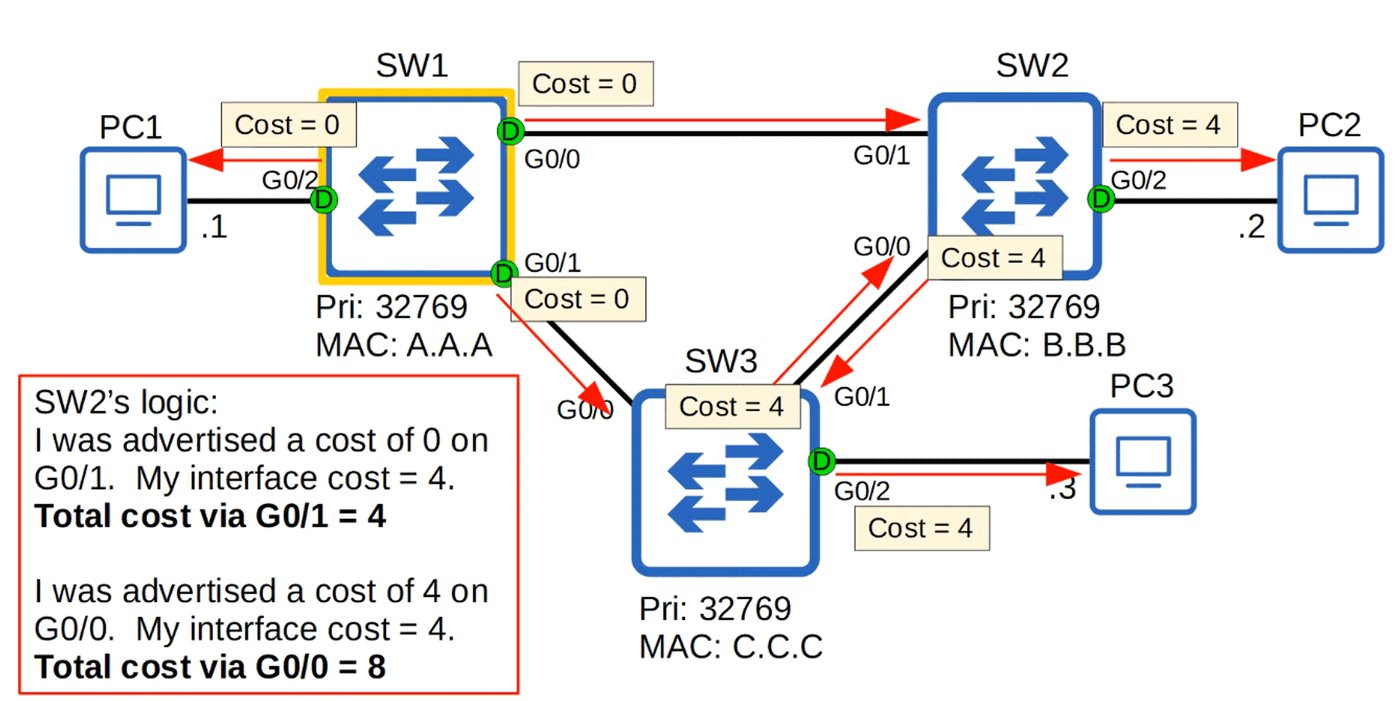
\includegraphics[keepaspectratio,alt={image}]{images/21-spanning-tree-protocol-part1/img-014.png}}
\end{figure}

The PORTS connected to another SWITCH's ROOT PORT MUST be DESIGNATED
(D).

Because the ROOT PORT Is the SWITCH's path to the ROOT BRIDGE, another
SWITCH must not block it.

STP PORT ID (in case of a tie-breaker)

\begin{figure}
\centering
\pandocbounded{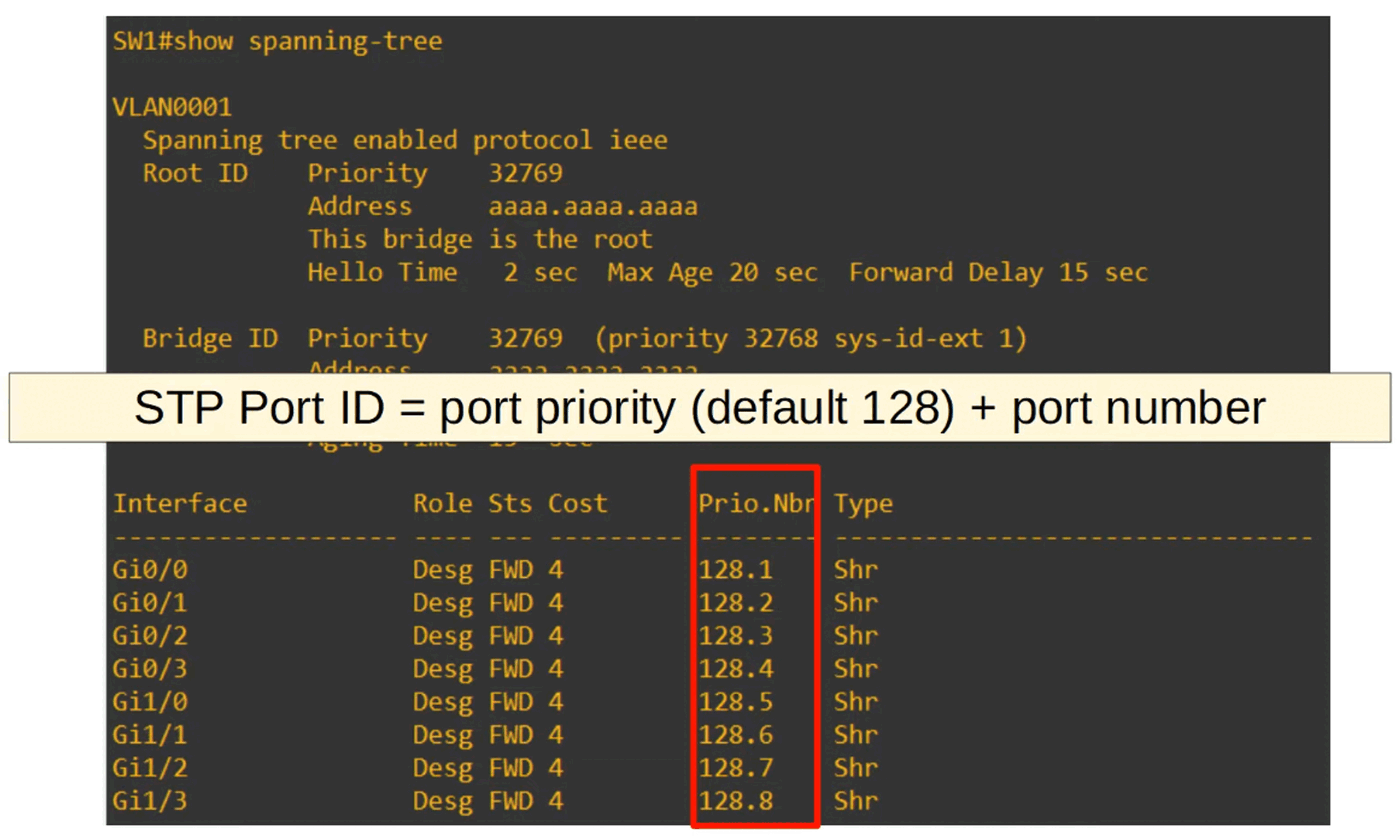
\includegraphics[keepaspectratio,alt={image}]{images/21-spanning-tree-protocol-part1/img-015.png}}
\end{figure}

NEIGHBOUR SWITCH PORT ID (in case of a tie-breaker)

\begin{enumerate}
\def\labelenumi{(\Alph{enumi})}
\setcounter{enumi}{3}
\item
  = DESIGNATED PORT
\item
  = ROOT PORT
\end{enumerate}

\begin{figure}
\centering
\pandocbounded{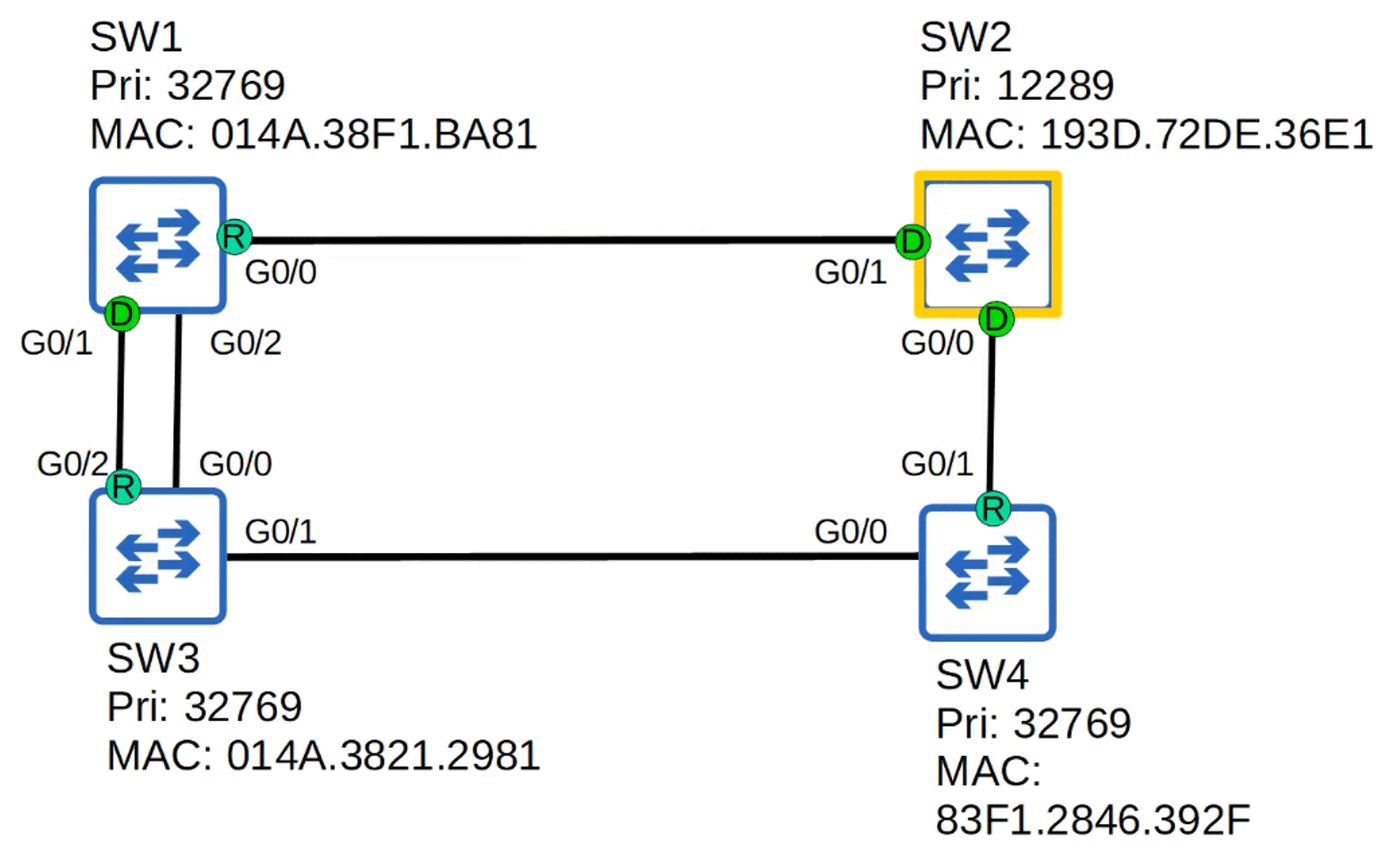
\includegraphics[keepaspectratio,alt={image}]{images/21-spanning-tree-protocol-part1/img-016.png}}
\end{figure}

\section{How to Determine Which Port Will Be Blocked to Prevent Layer 2
Loops}\label{how-to-determine-which-port-will-be-blocked-to-prevent-layer-2-loops}

\begin{figure}
\centering
\pandocbounded{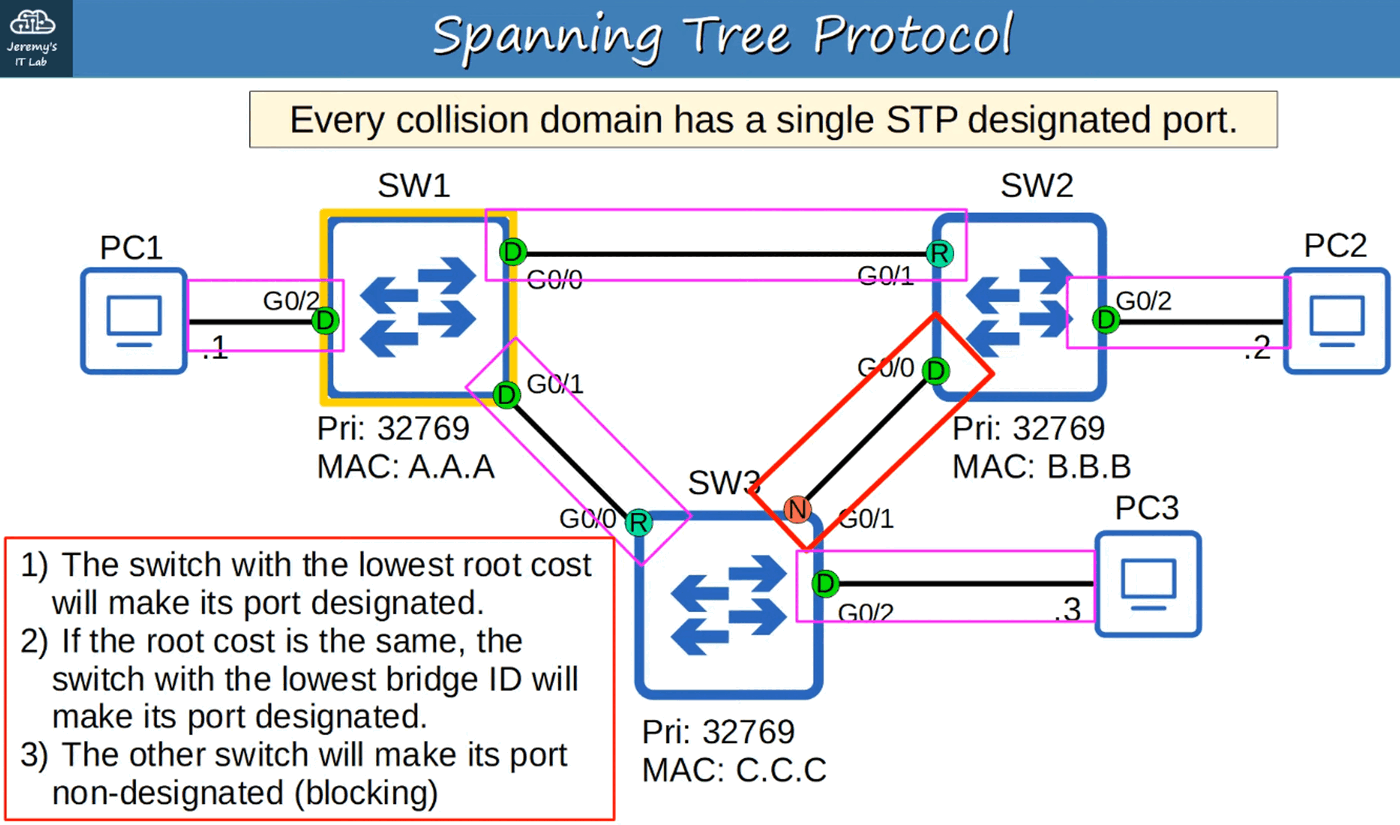
\includegraphics[keepaspectratio,alt={image}]{images/21-spanning-tree-protocol-part1/img-017.png}}
\end{figure}

\section{Quiz}\label{quiz}

Identify the ROOT BRIDGE and the ROLE of EACH INTERFACE on the NETWORK
(ROOT / DESIGNATED / NON-DESIGNATED)

\#1

\begin{figure}
\centering
\pandocbounded{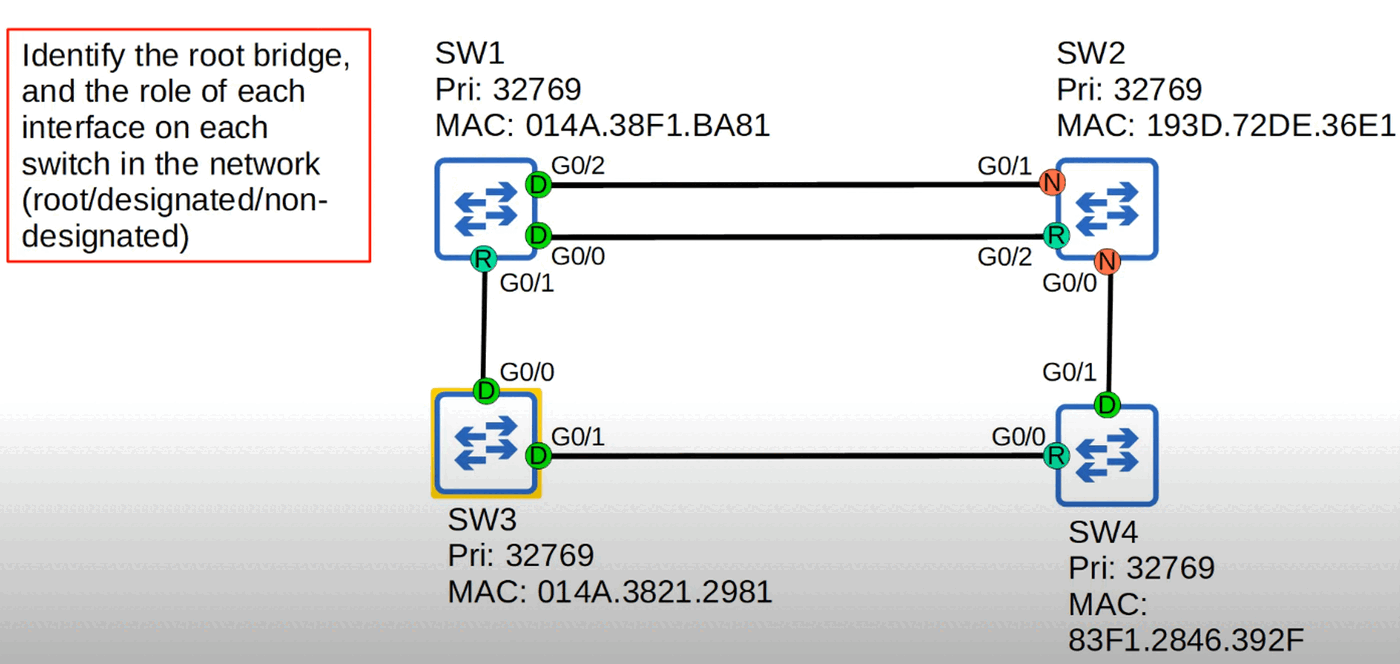
\includegraphics[keepaspectratio,alt={image}]{images/21-spanning-tree-protocol-part1/img-018.png}}
\end{figure}

ALL SWITCHES have the same PRIORITY NUMBER (32769)

Tie-breaker goes to the LOWEST MAC ADDRESS

SW3 has the LOWEST so it's the ROOT BRIDGE and ALL it's INTERFACES
become DESIGNATED

Connections from SW1 (G0/1) and S4 (G0/0) to SW3 become ROOT INTERFACES

Because SW2 has TWO connections to SW1, both of SW1's INCOMING
interfaces become DESIGNATED.

SW2 G0/2 INTERFACE becomes a ROOT INTERFACE because the G0/0 INTERFACE
of SW1 is LOWER than it's G0/2 INTERFACE

The remaining interfaces on SW2 become NON-DESIGNATED because it has the
HIGHEST ROOT COST (12 = 4x 1 GB connection). INTERFACES they are
attached to on other SWITCHES become DESIGNATED

\#2

\begin{figure}
\centering
\pandocbounded{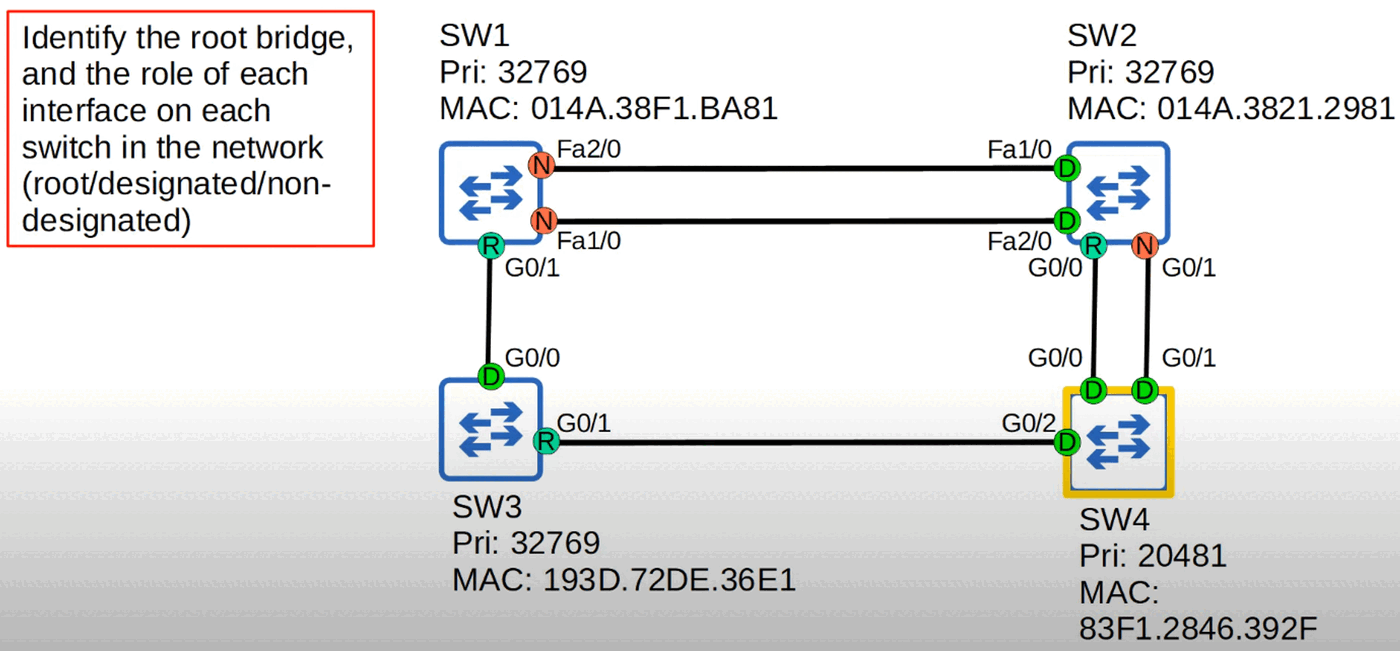
\includegraphics[keepaspectratio,alt={image}]{images/21-spanning-tree-protocol-part1/img-019.png}}
\end{figure}

SW4 has the LOWEST Priority Number so it is designated ROOT BRIDGE

All of SW4 INTERFACES become DESIGNATED

SW2 G0/0 becomes ROOT PORT because SW4 G0/0 connection is a LOWER NUMBER
than G0/1.

SW3 G0/1 becomes ROOT PORT

SW1 G0/1 becomes ROOT PORT because G0/1 cost is LESS than Fa1/0 and 2/0

EACH remaining PORT will be either DESIGNATED or NON-DESIGNATED

SW1 Fa1/0 and 2/0 become NON-DESIGNATED since they have a HIGHER STP
COST (38) than SW2 outbound ports (8) making SW2 Fa1/0 and 2/0
DESIGNATED

SW2 remaining connection, G0/1, NON-DESIGNATED

\chapter{Spanning Tree Protocol: Part
2}\label{spanning-tree-protocol-part-2}

\section{STP States}\label{stp-states}

\begin{figure}
\centering
\pandocbounded{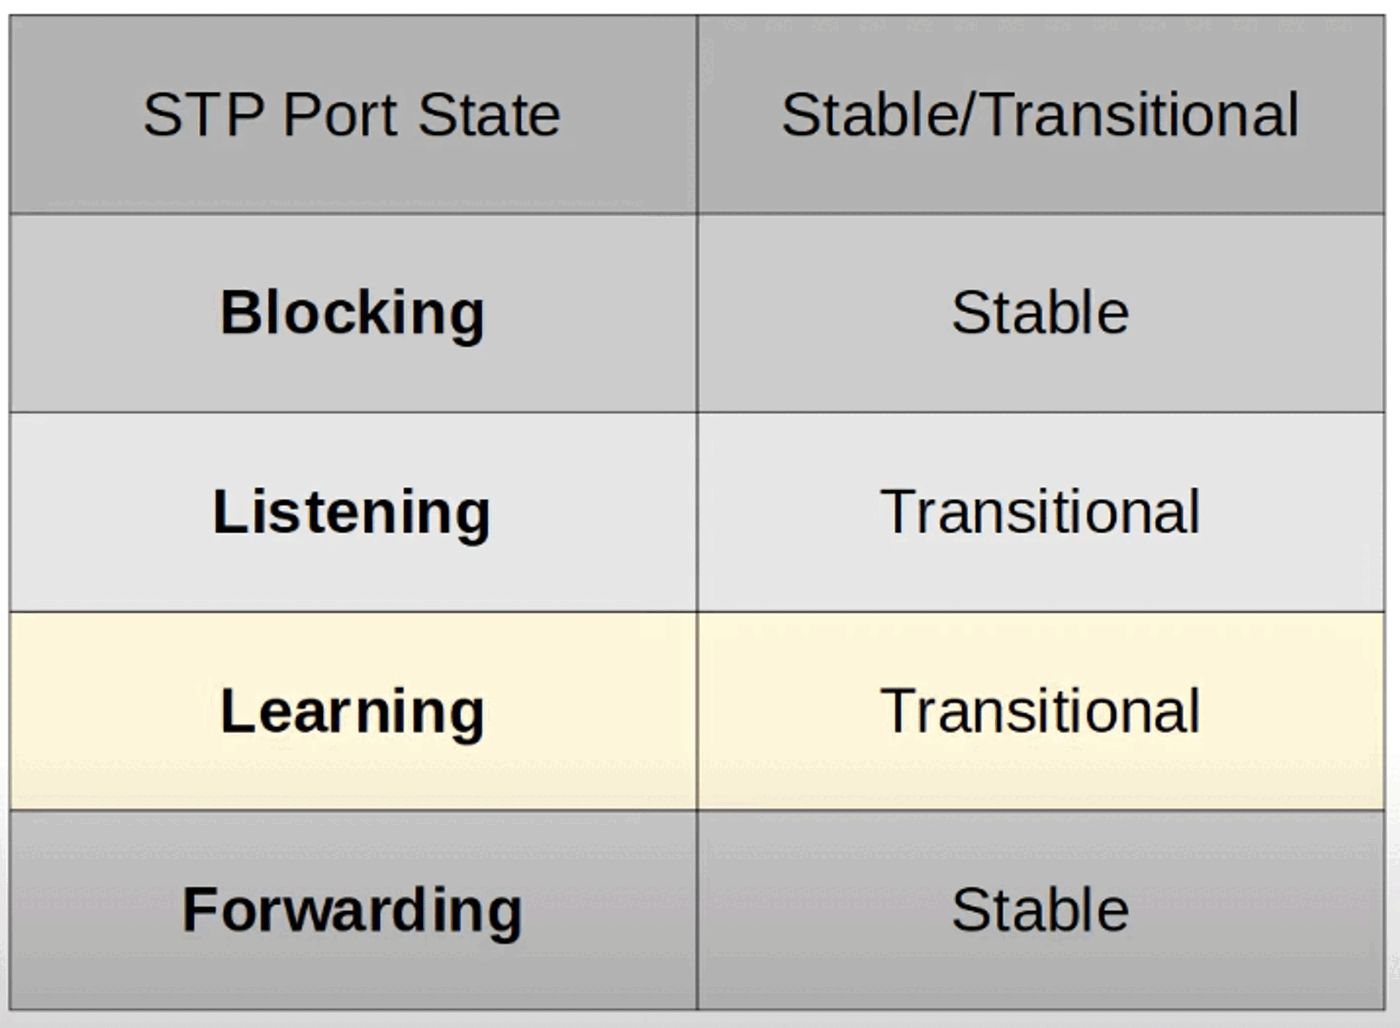
\includegraphics[keepaspectratio,alt={image}]{images/22-spanning-tree-protocol-part2/img-001.png}}
\end{figure}

\begin{itemize}
\tightlist
\item
  ROOT / DESIGNATED PORTS remain STABLE in a FORWARDING state
\item
  NON-DESIGNATED PORTS remain STABLE in a BLOCKING state
\item
  LISTENING and LEARNING are TRANSITIONAL states which are passed
  through when an interface is activated, or when a BLOCKING PORT must
  transition to a FORWARDING state due to a change in network topology.
\end{itemize}

\textbf{1) BLOCKING / STABLE}

\begin{itemize}
\tightlist
\item
  NON-DESIGNATED PORTS are in a BLOCKING state
\item
  Interfaces in a BLOCKING state are effectively disabled to prevent
  loops
\item
  Interfaces in a BLOCKING state do NOT Send/Receive regular network
  traffic
\item
  Interfaces in a BLOCKING state do NOT forward STP BPDUs
\item
  Interfaces in a BLOCKING state do NOT learn MAC ADDRESSES
\end{itemize}

\textbf{2) LISTENING / TRANSITIONAL}

\begin{itemize}
\tightlist
\item
  After the BLOCKING state, interfaces with the DESIGNATED or ROOT role
  enter the LISTENING state
\item
  ONLY DESIGNATED or ROOT PORTS enter the LISTENING state
  (NON-DESIGNATED PORTS are ALWAYS BLOCKING)
\item
  The LISTENING state is 15 seconds long by Default. This is determined
  by the FORWARD DELAY TIMER
\item
  Interfaces in a LISTENING state do NOT Send / Receive regular network
  traffic
\item
  Interfaces in a LISTENING state ONLY Forward/Receive STP BPDUs
\item
  Interfaces in a LISTENING state does NOT learn MAC ADDRESSES from
  regular traffic that arrives on the interface
\end{itemize}

\textbf{3) LEARNING / TRANSITIONAL}

\begin{itemize}
\tightlist
\item
  After the LISTENING state, a DESIGNATED or ROOT port will enter the
  LEARNING state
\item
  The LEARNING state is 15 seconds long by Default. This is determined
  by the FORWARD DELAY TIMER (same one used for both LISTENING and
  LEARNING states)
\item
  Interfaces in a LEARNING state do NOT Send / Receive regular network
  traffic
\item
  Interfaces in a LEARNING state ONLY Sends/Receives STP BPDUs
\item
  Interfaces in a LEARNING state \textbf{learns} MAC ADDRESSES from
  regular traffic that arrives on the interface
\end{itemize}

\begin{enumerate}
\def\labelenumi{\arabic{enumi})}
\setcounter{enumi}{3}
\tightlist
\item
  FORWARDING / STABLE
\end{enumerate}

\begin{itemize}
\tightlist
\item
  ROOT and DESIGNATED PORTS are in a FORWARDING state
\item
  A PORT in the FORWARDING state operate as NORMAL
\item
  A PORT in the FORWARDING state Sends/Receives regular network traffic
\item
  A PORT in the FORWARDING state Sends/Receives STP BPDUs
\item
  A PORT in the FORWARDING state \textbf{learns} MAC ADDRESSES
\end{itemize}

\section{Summary}\label{summary}

\begin{figure}
\centering
\pandocbounded{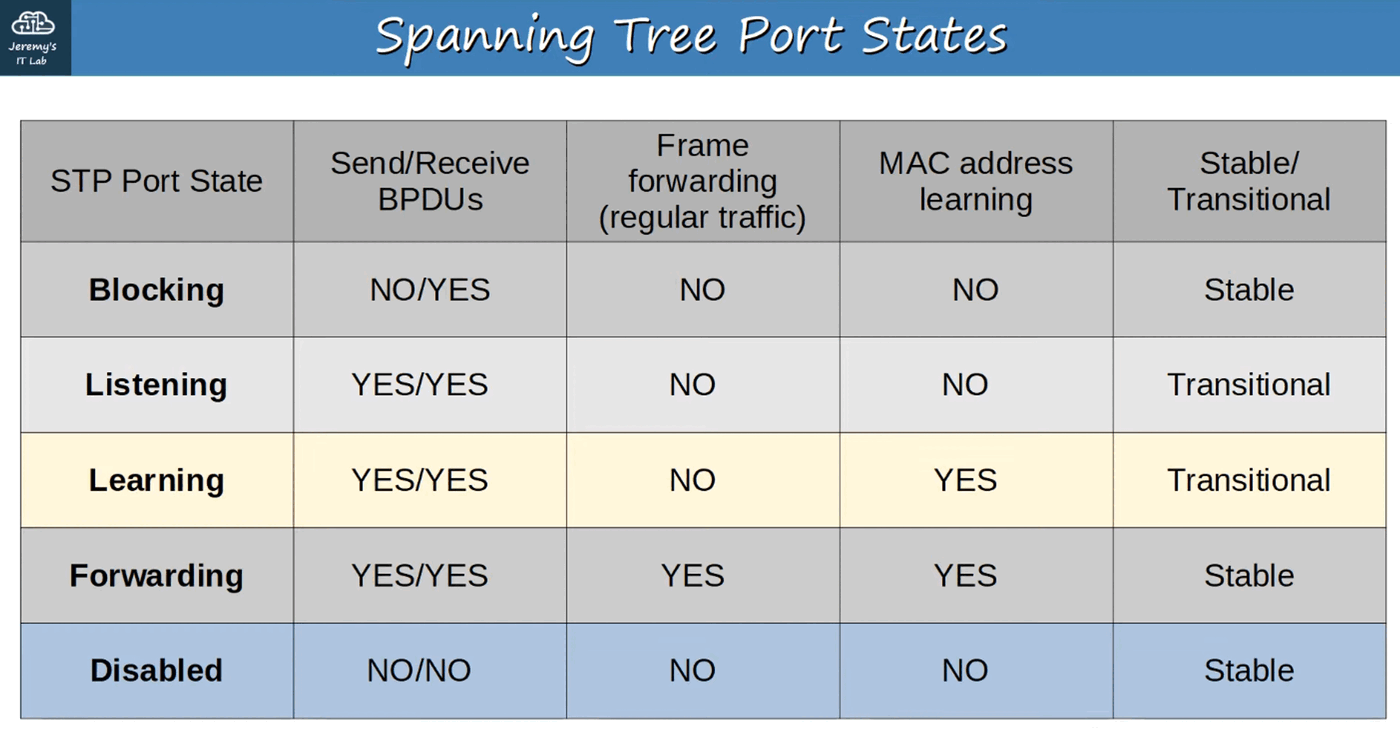
\includegraphics[keepaspectratio,alt={image}]{images/22-spanning-tree-protocol-part2/img-002.png}}
\end{figure}

\section{STP Timers}\label{stp-timers}

\begin{figure}
\centering
\pandocbounded{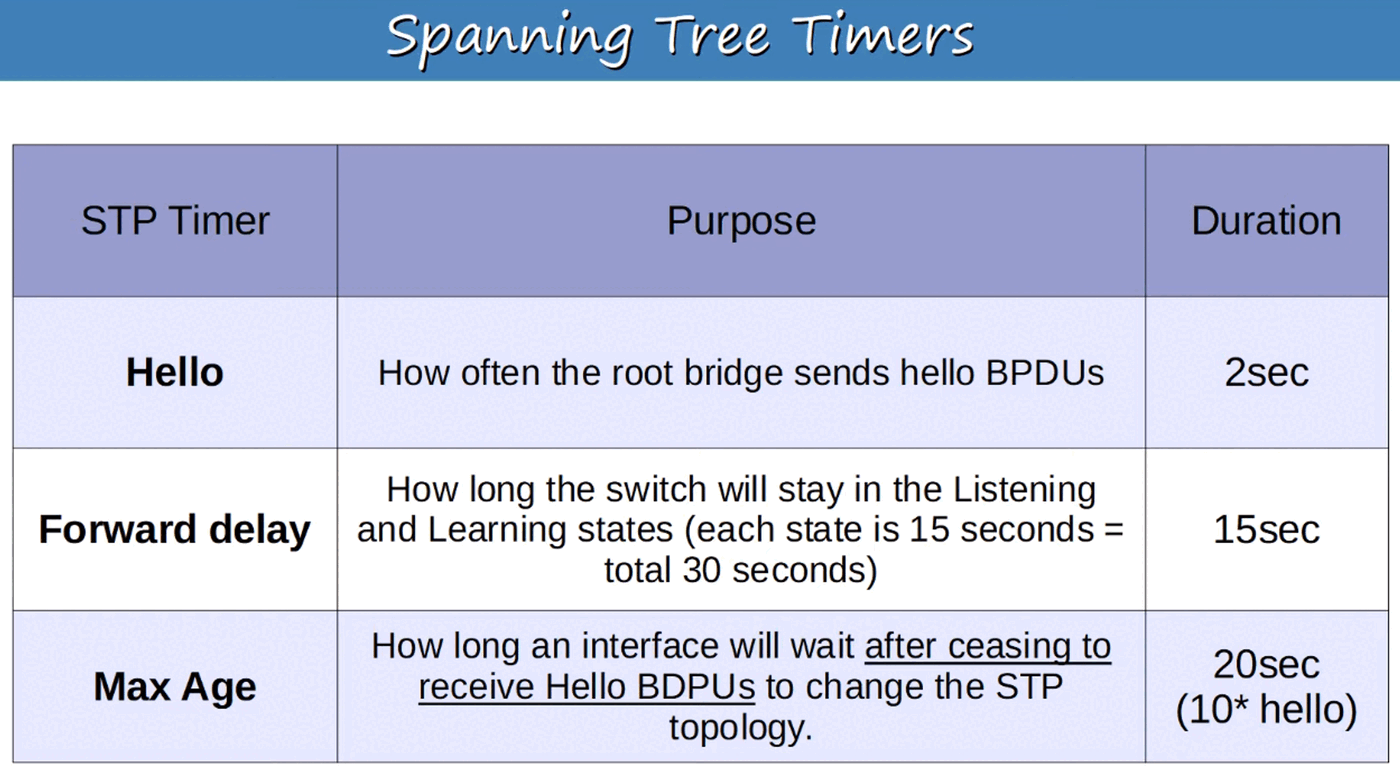
\includegraphics[keepaspectratio,alt={image}]{images/22-spanning-tree-protocol-part2/img-003.png}}
\end{figure}

SWITCHES do NOT forward the BPDUs out of their ROOT PORTS and
NON-DESIGNATED PORTS - ONLY their DESIGNATED PORTS !!!

\section{Max Age Timer}\label{max-age-timer}

\begin{itemize}
\tightlist
\item
  If another BPDU is received BEFORE MAX AGE TIMER counts down to 0, the
  TIME will RESET to 20 Seconds and no changes will occur.
\item
  If another BPDU is not received, the MAX AGE TIMER counts down to 0
  and the SWITCH will re-evaluate it's STP choices, including ROOT
  BRIDGE, LOCAL ROOT, DESIGNATED, and NON-DESIGNATED PORTS.
\item
  If a NON-DESIGNATED PORT is selected to become a DESIGNATED or ROOT
  PORT, it will transition from the BLOCKING state to the LISTENING
  state (15 Seconds), LEARNING state (15 Seconds), and then finally the
  FORWARDING state.

  \begin{itemize}
  \tightlist
  \item
    So\ldots{} it can take 50 Seconds for a BLOCKING interface to
    transition to FORWARDING! (MAX AGE TIMER + (LISTENING + LEARNING 15
    Second timers))
  \end{itemize}
\item
  These TIMERS and TRANSITIONAL STATES are to make sure that LOOPS are
  not accidentally created by an INTERFACE moving to FORWARDING STATE
  too soon
\end{itemize}

HOWEVER \ldots{}

A FORWARDING interface can move DIRECTLY to a BLOCKING state (there is
no worry about creating a loop)

A BLOCKING interface can NOT move DIRECTLY to a FORWARDING state. It
MUST go through the LISTENING and LEARNING states first!

\section{STP BPDU (Bridge Protocol Data
Unit)}\label{stp-bpdu-bridge-protocol-data-unit}

Ethernet Header of a BPDU

\begin{figure}
\centering
\pandocbounded{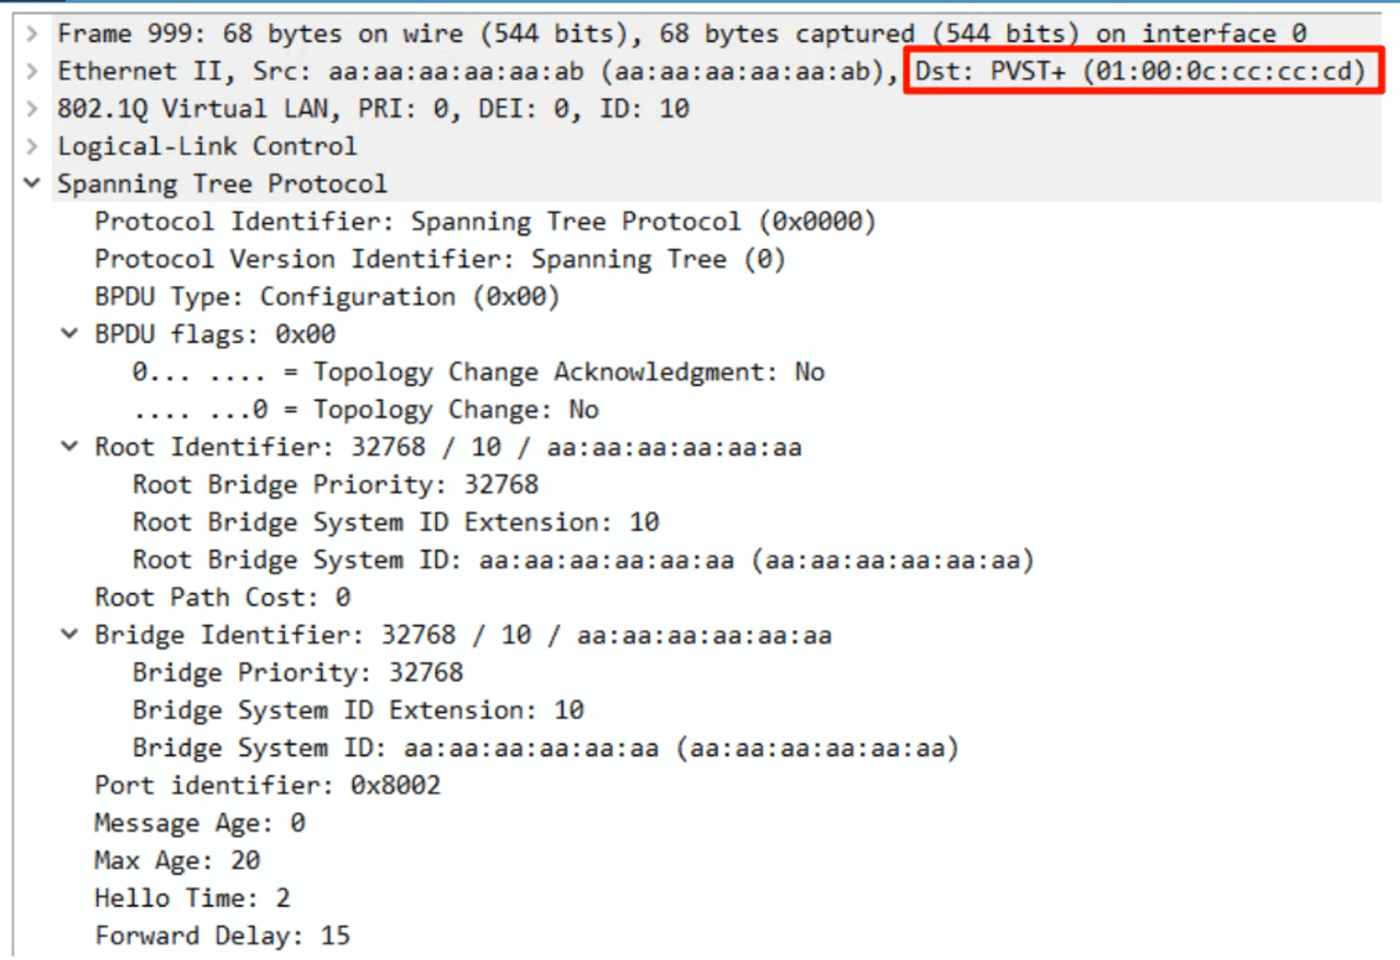
\includegraphics[keepaspectratio,alt={image}]{images/22-spanning-tree-protocol-part2/img-004.png}}
\end{figure}

PVST+ uses the MAC ADDRESS :

01 : 00 : 0c : cc : cc : cd

PVST = ONLY ISL Trunk Encapsulation

PVST+ = Supports 802.1Q

Regular STP (not Cisco's PVST+) uses the MAC ADDRESS :

01 : 80 : c2 : 00 : 00 : 00

The STP TIMERS on the ROOT BRIDGE determine ALL STP TIMERS for the
entire network!

\section{STP Optional Features (STP
Toolkit)}\label{stp-optional-features-stp-toolkit}

\section{Portfast}\label{portfast}

\begin{itemize}
\tightlist
\item
  Can be Enabled on INTERFACES which are connected to END HOSTS
\end{itemize}

PORTFAST allows a PORT to move immediately to the FORWARDING state,
bypassing LISTENING and LEARNING

\begin{itemize}
\tightlist
\item
  If used, it MUST be ENABLED only on PORTS connected to END HOSTS
\item
  If ENABLED on a PORT connected to another SWITCH, it could cause a
  LAYER 2 LOOP
\end{itemize}

\begin{figure}
\centering
\pandocbounded{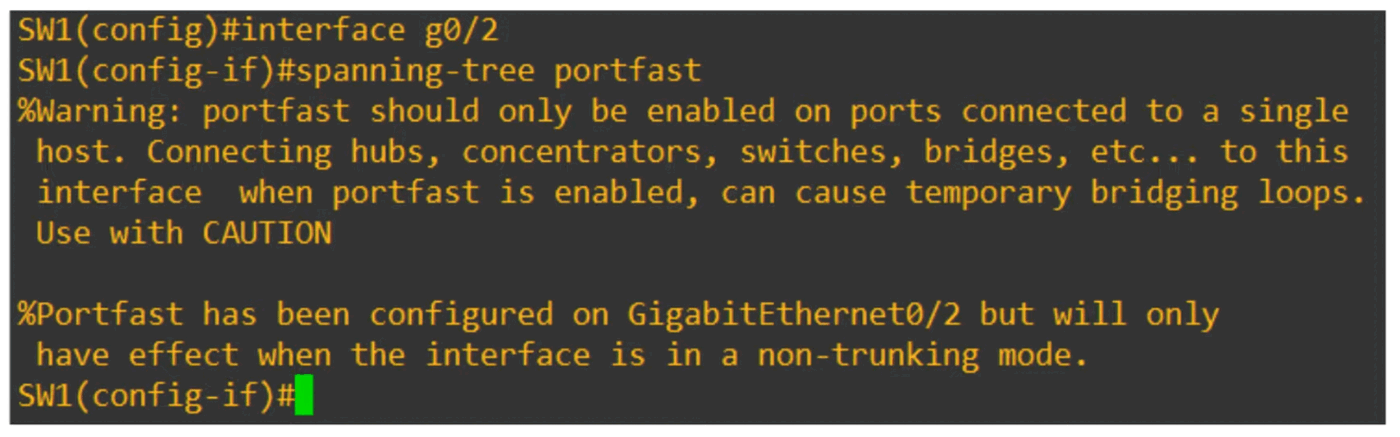
\includegraphics[keepaspectratio,alt={image}]{images/22-spanning-tree-protocol-part2/img-005.png}}
\end{figure}

You can also ENABLE PORTFAST with the following command:

SW1(config)\# spanning-tree portfast default

This ENABLES PORTFAST on ALL ACCESS PORTS (not TRUNK PORTS)

\section{BPDU Guard}\label{bpdu-guard}

\begin{itemize}
\tightlist
\item
  If an INTERFACE with BPDU GUARD ENABLED receives a BPDU from another
  SWITCH, the INTERFACE will be SHUT DOWN to prevent loops from forming.
\end{itemize}

\begin{figure}
\centering
\pandocbounded{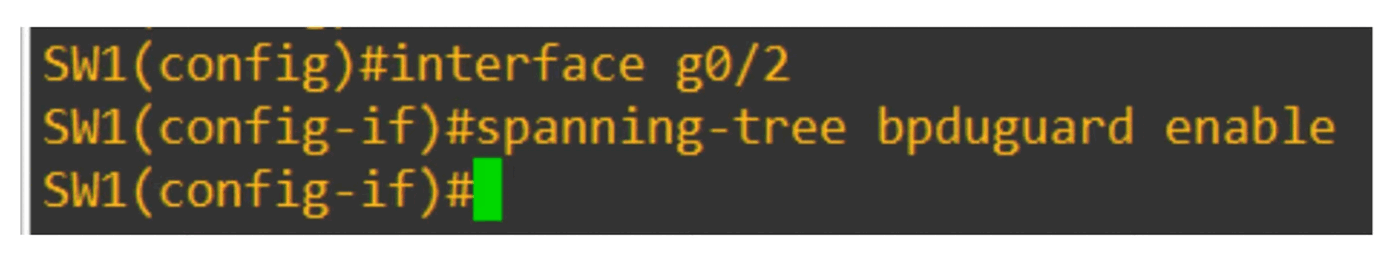
\includegraphics[keepaspectratio,alt={image}]{images/22-spanning-tree-protocol-part2/img-006.png}}
\end{figure}

You can also ENABLE BPDU GUARD with the following command:

SW1(config)\# spanning-tree portfast bpduguard default

This ENABLES BPDU GUARD on all PORTFAST-enabled INTERFACES

\section{Root Guard / Loop Guard}\label{root-guard-loop-guard}

\begin{figure}
\centering
\pandocbounded{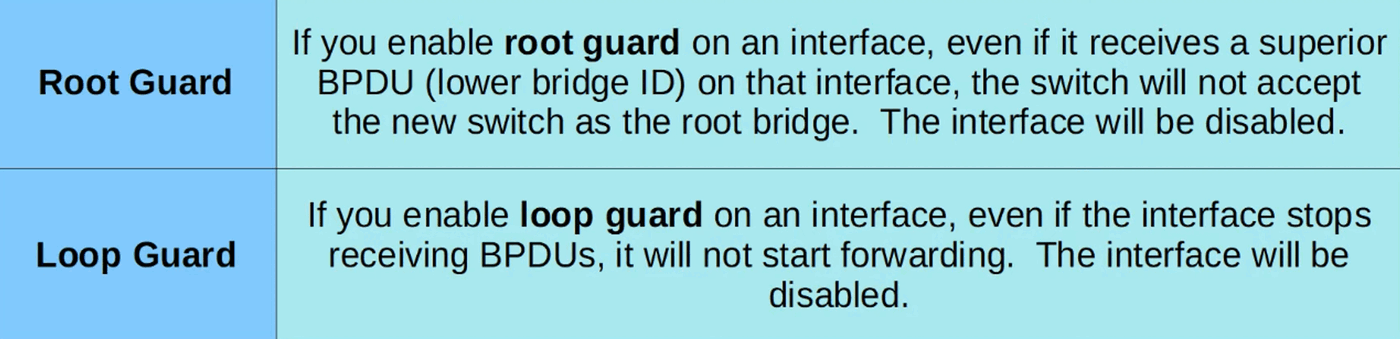
\includegraphics[keepaspectratio,alt={image}]{images/22-spanning-tree-protocol-part2/img-007.png}}
\end{figure}

You probably do NOT have to know these STP optional features (or others
such as UplinkFast, Backbone Fast, etcetera) for the CCNA.

BUT\ldots{}

Make sure you know PORTFAST and BPDU GUARD.

\section{STP Configuration}\label{stp-configuration}

Command to CONFIGURE Spanning-Tree mode on a SWITCH

\begin{figure}
\centering
\pandocbounded{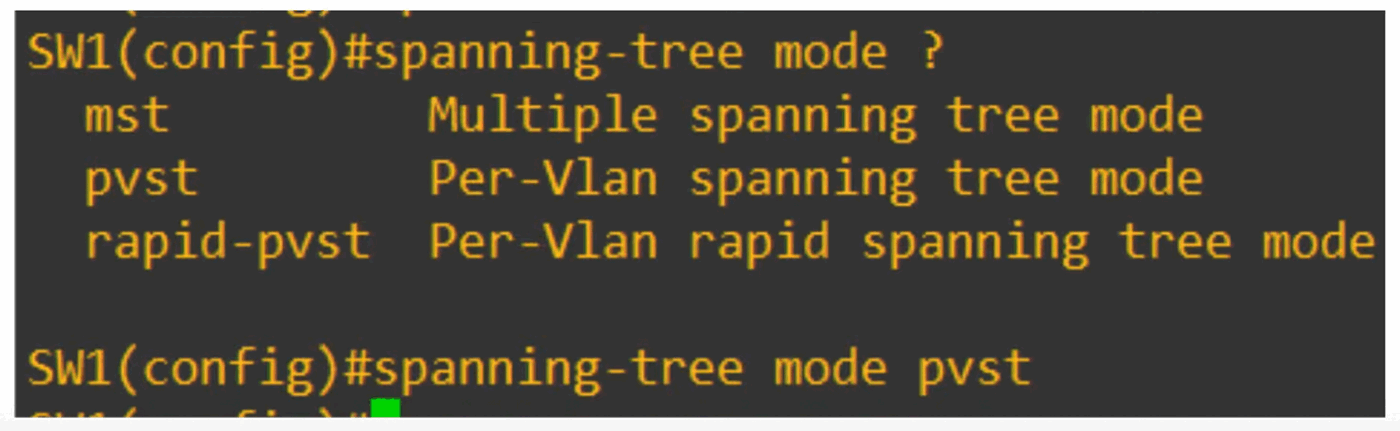
\includegraphics[keepaspectratio,alt={image}]{images/22-spanning-tree-protocol-part2/img-008.png}}
\end{figure}

Modern Cisco SWITCHES run \textbf{rapid-pvst}, by default

\section{Configure the Primary Root
Bridge}\label{configure-the-primary-root-bridge}

Command to CONFIGURE Spanning-Tree PRIMARY ROOT BRIDGE on a SWITCH

\begin{figure}
\centering
\pandocbounded{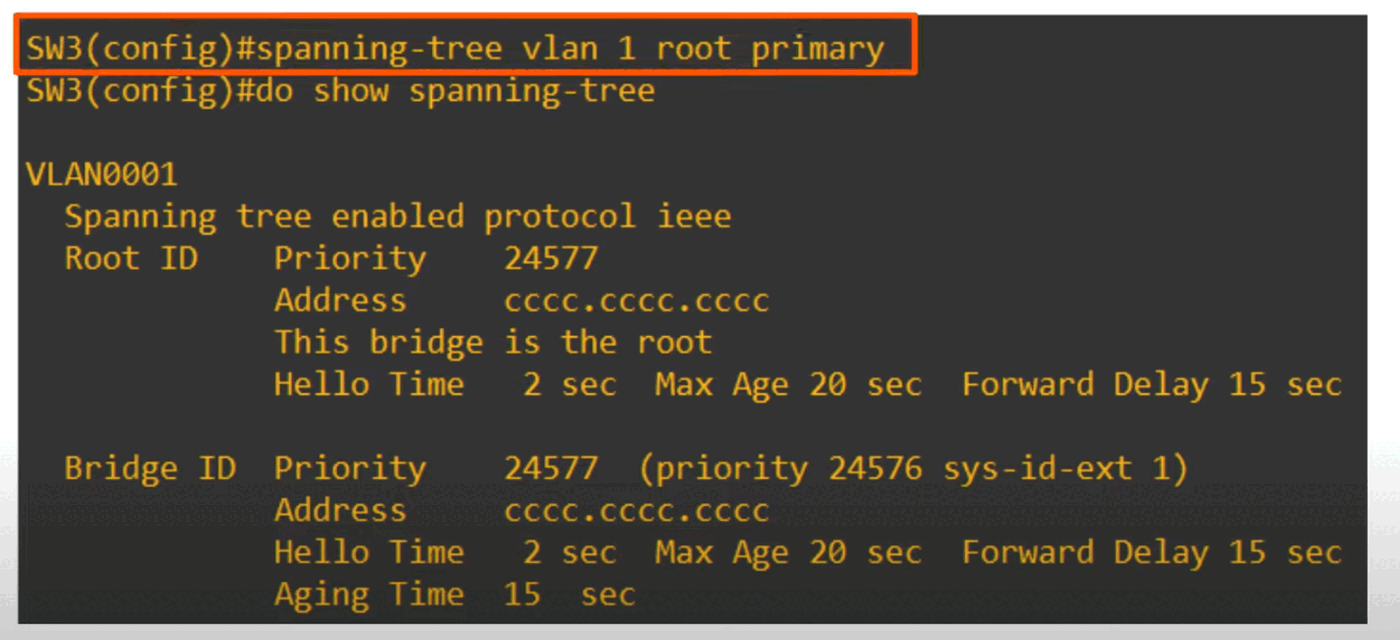
\includegraphics[keepaspectratio,alt={image}]{images/22-spanning-tree-protocol-part2/img-009.png}}
\end{figure}

Confirm with ``(do) show spanning-tree''

Can see in the above example, SW3 has become the ``root''

\begin{itemize}
\tightlist
\item
  The ``spanning-tree vlan \textless vlan-number\textgreater{} root
  primary'' command sets the STP PRIORITY to 24576. If another SWITCH
  already has a priority number lower than 24576, it sets this SWITCH's
  priority to 4096 LESS THAN the other SWITCH's Priority (remember STP
  PART 1 lecture)
\end{itemize}

SECONDARY ROOT BRIGE (backup ROOT BRIDGE)

Command to CONFIGURE Spanning-Tree SECONDARY ROOT BRIDGE on a SWITCH

\begin{figure}
\centering
\pandocbounded{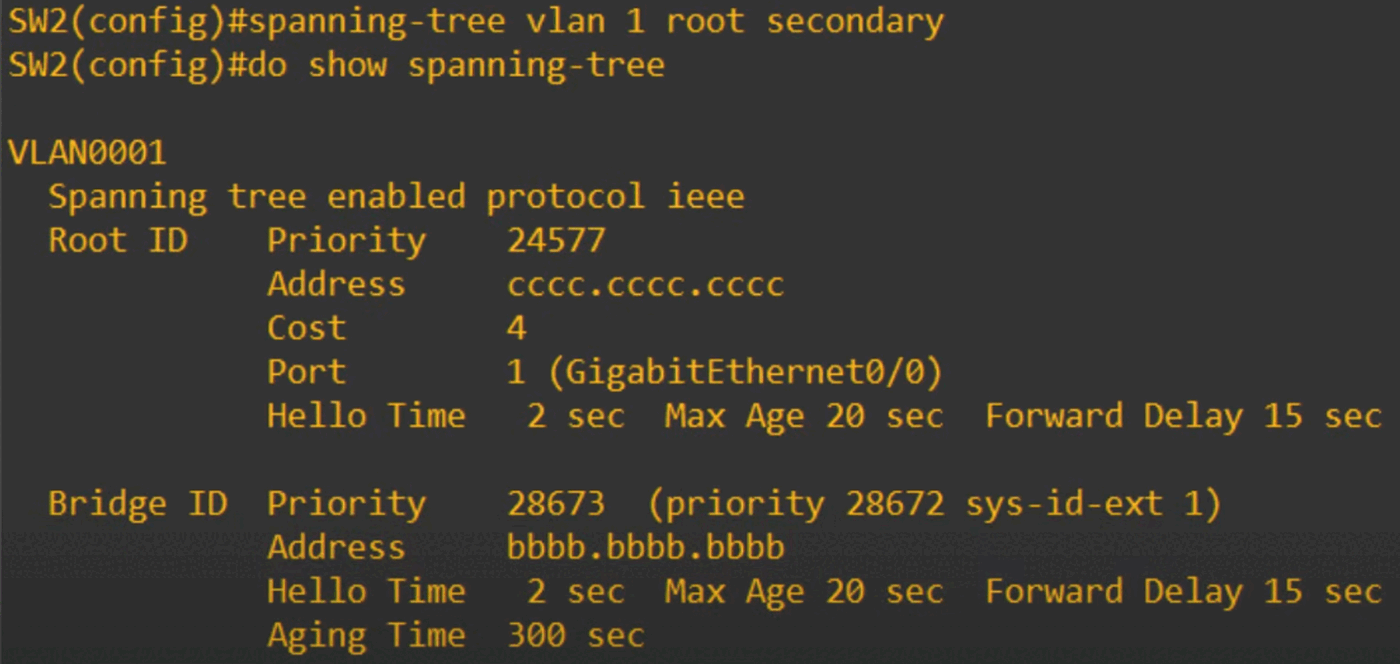
\includegraphics[keepaspectratio,alt={image}]{images/22-spanning-tree-protocol-part2/img-010.png}}
\end{figure}

\begin{itemize}
\tightlist
\item
  The ``spanning-tree vlan \textless vlan-number\textgreater{} root
  secondary'' command sets the STP PRIORITY to 28672 (exactly 4096
  higher than 24576).
\end{itemize}

VLAN 1 TOPOLOGY running PVST+

\begin{figure}
\centering
\pandocbounded{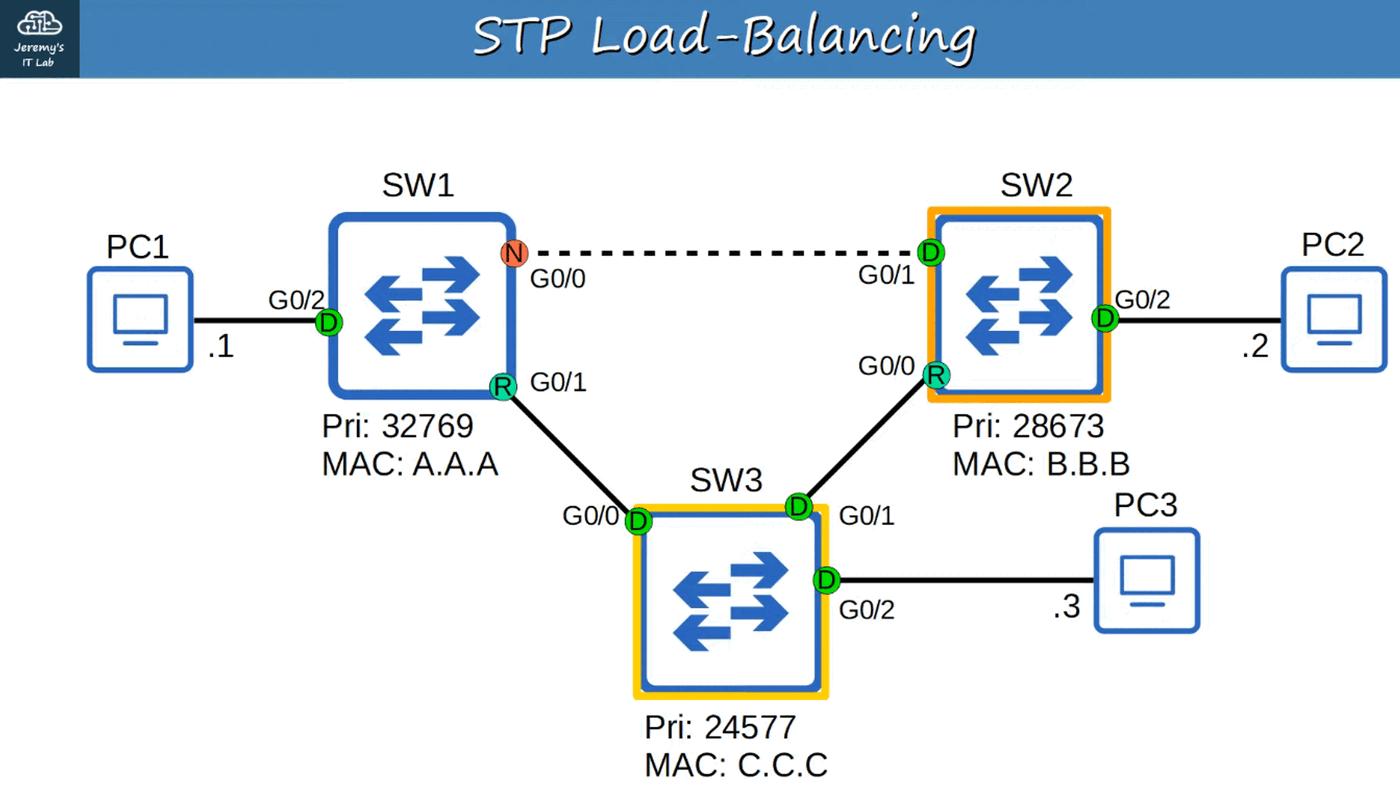
\includegraphics[keepaspectratio,alt={image}]{images/22-spanning-tree-protocol-part2/img-011.png}}
\end{figure}

SW1 WAS the PRIMARY ROOT BRIDGE but :

\begin{itemize}
\tightlist
\item
  We have configured SW3 to be the PRIMARY
\item
  We have configured SW2 to be the SECONDARY
\end{itemize}

The TOPOLOGY for VLAN 2, however, won't be the same. It will be the OLD
Topology.

\begin{figure}
\centering
\pandocbounded{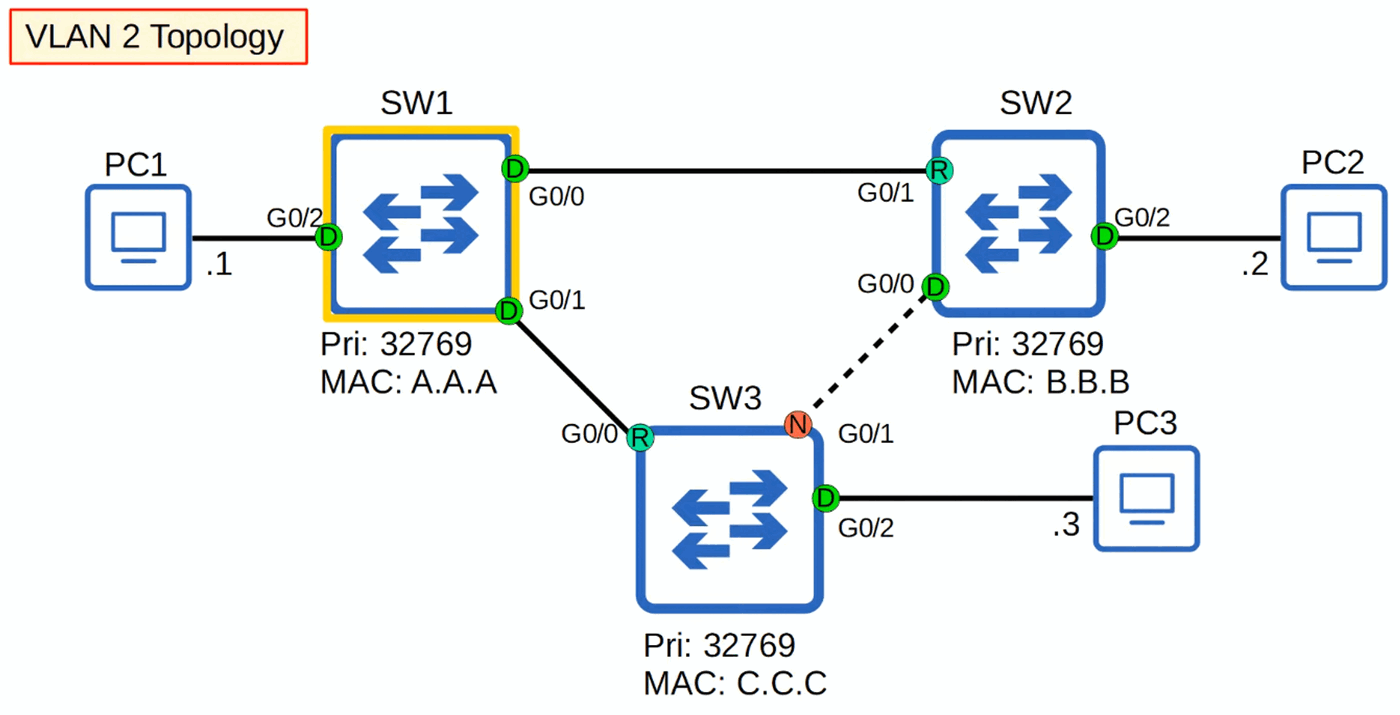
\includegraphics[keepaspectratio,alt={image}]{images/22-spanning-tree-protocol-part2/img-012.png}}
\end{figure}

WHY? Because we made changes ONLY to the TOPOLOGY found in VLAN 1 (see
the commands we used)

\section{Configure STP Port Settings}\label{configure-stp-port-settings}

\begin{figure}
\centering
\pandocbounded{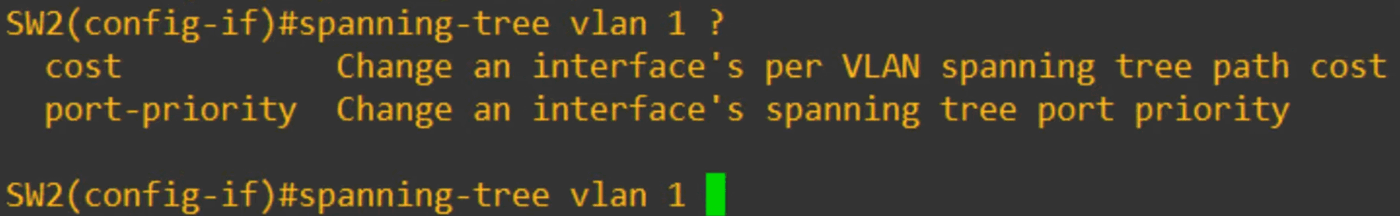
\includegraphics[keepaspectratio,alt={image}]{images/22-spanning-tree-protocol-part2/img-013.png}}
\end{figure}

``cost'' = ``ROOT COST''

``port-priority'' = ``PORT PRIORITY''

\chapter{Rapid Spanning Tree
Protocol}\label{rapid-spanning-tree-protocol}

\emph{COMPARISON OF STP VERSIONS (Standard vs.~Cisco)}

\begin{figure}
\centering
\pandocbounded{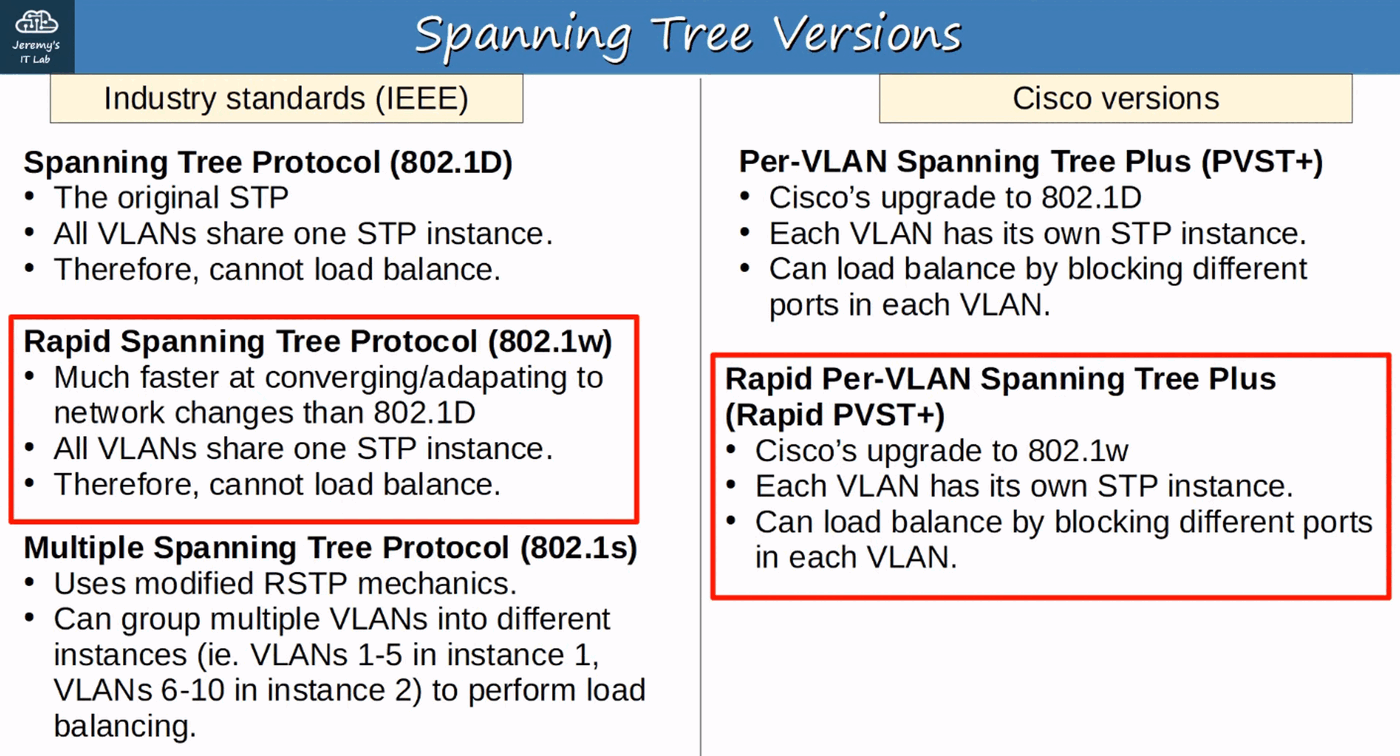
\includegraphics[keepaspectratio,alt={image}]{images/23-rapid-spanning-tree-protocol/img-001.png}}
\end{figure}

We are only concerned with 802.1w for MOST use cases.

MSTP (802.1s) is more useful for VERY LARGE networks.

WHAT IS RAPID PER-VLAN SPANNING TREE PLUS?

\begin{quote}
RSTP is not a time-based spanning tree algorithm like 802.1D. Therefore,
RSTP offers an improvment over teh 30 seconds or more 802.1D takes to
move a link to forwarding. The heart of the protocol is a new
bridge-bridge handshake mechanism, which allows ports to move directly
to forwarding
\end{quote}

\section{Similarities Between STP and
RSTP}\label{similarities-between-stp-and-rstp}

\begin{itemize}
\tightlist
\item
  RSTP serves the same purpose as STP, blocking specific PORTS to
  prevent LAYER 2 LOOPS.
\item
  RSTP elects a ROOT BRIDGE with the same rules as STP
\item
  RSTP elects ROOT PORTS with the same rules as STP
\item
  RSTP elects DESIGNATED PORTS with the same rules as STP
\end{itemize}

\section{Differences Between STP and
RSTP}\label{differences-between-stp-and-rstp}

\textbf{PORT COSTS}

\begin{figure}
\centering
\pandocbounded{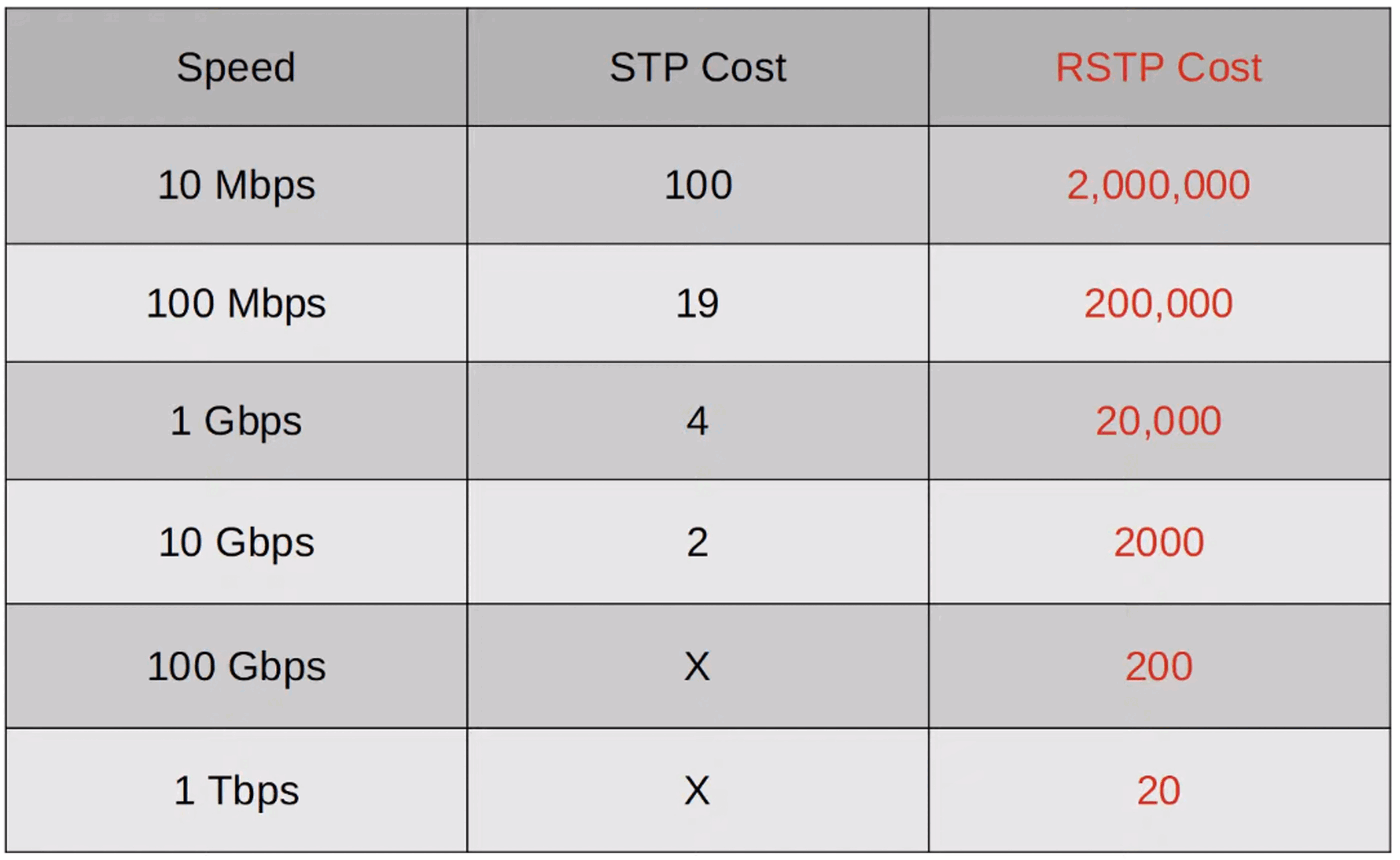
\includegraphics[keepaspectratio,alt={image}]{images/23-rapid-spanning-tree-protocol/img-002.png}}
\end{figure}

(STUDY AND MEMORIZE PORT COSTS OF STP AND RSTP)

\section{RSTP Port States}\label{rstp-port-states}

\begin{figure}
\centering
\pandocbounded{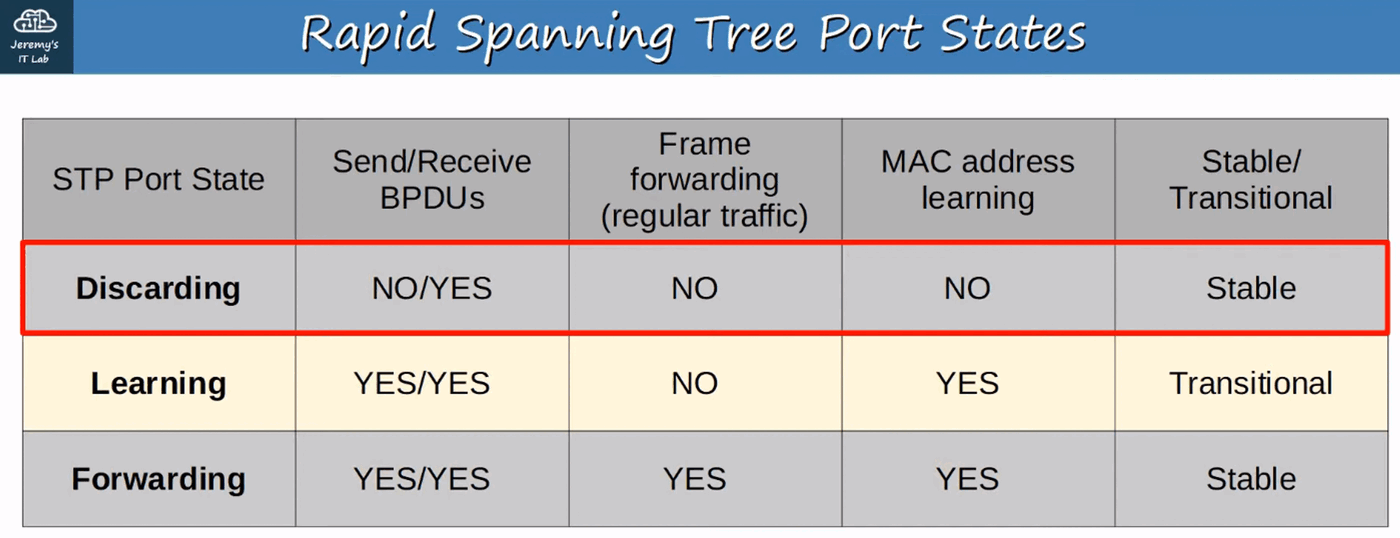
\includegraphics[keepaspectratio,alt={image}]{images/23-rapid-spanning-tree-protocol/img-003.png}}
\end{figure}

\begin{itemize}
\tightlist
\item
  If a PORT has been ADMINISTRATIVELY DISABLED (''shutdown'' command) =
  DISCARDING STATE
\item
  If a PORT is ENABLED but BLOCKING traffic to prevent LAYER 2 LOOPS =
  DISCARDING STATE
\end{itemize}

\section{RSTP Roles}\label{rstp-roles}

\begin{itemize}
\tightlist
\item
  The ROOT PORT role remains unchanged in RSTP

  \begin{itemize}
  \tightlist
  \item
    The PORT that is closest to the ROOT BRIDGE becomes the ROOT PORT
    for the SWITCH
  \item
    The ROOT BRIDGE is the only SWITCH that doesn't have a ROOT PORT
  \end{itemize}
\item
  The DESIGNATED PORT role remains unchanged in RSTP

  \begin{itemize}
  \tightlist
  \item
    The PORT on a segment (Collision Domain) that sends the best BPDU is
    that segment's DESIGNATED PORT (only one per segment!)
  \end{itemize}
\item
  The NON-DESIGNATED PORT role is split into TWO separate roles in RSTP:

  \begin{itemize}
  \tightlist
  \item
    The ALTERNATE PORT role
  \item
    The BACKUP PORT role
  \end{itemize}
\end{itemize}

\textbf{RSTP : ALTERNATE PORT ROLE}

\begin{itemize}
\tightlist
\item
  The RSTP ALTERNATE PORT ROLE is a DISCARDING PORT that receives a
  superior BPDU from another SWITCH
\item
  This is the same as what you've learned about BLOCKING PORTS in
  classic STP
\end{itemize}

\begin{figure}
\centering
\pandocbounded{\includegraphics[keepaspectratio,alt={image}]{images/23-rapid-spanning-tree-protocol/img-004.png}}
\end{figure}

\begin{itemize}
\tightlist
\item
  An ALTERNATE PORT (labelled ``A'' above) functions as a backup to the
  ROOT PORT
\item
  If the ROOT PORT fails, the SWITCH can immediately move it's best
  alternate port to FORWARDING
\end{itemize}

\begin{figure}
\centering
\pandocbounded{\includegraphics[keepaspectratio,alt={image}]{images/23-rapid-spanning-tree-protocol/img-005.png}}
\end{figure}

This immediate move to FORWARDING STATE functions like a classic STP
optional feature called \textbf{UplinkFast.} Because it is built into
RSTP, you do not need to activate UplinkFast when using RSTP/Rapid PVST+

One more STP optional feature that was built into RSTP is
\textbf{BackboneFast}

\begin{figure}
\centering
\pandocbounded{\includegraphics[keepaspectratio,alt={image}]{images/23-rapid-spanning-tree-protocol/img-006.png}}
\end{figure}

\begin{itemize}
\tightlist
\item
  \textbf{BackboneFast} allows SW3 to expire the MAX AGE TIMERS on it's
  INTERFACE and rapidly FORWARD the superior BPDUs to SW2
\item
  This FUNCTIONALITY is built into RSTP, so it does not need to be
  configured.
\end{itemize}

UPLINKFAST and BACKBONE FAST (SUMMARY)

\textbf{UplinkFast} and \textbf{BackboneFast} are two optional features
in Classic STP. They must be configured to operate on the SWITCH (not
necessary to know for the CCNA)

\begin{itemize}
\tightlist
\item
  Both features are built into RSTP, so you do NOT have to configure
  them. They operate, by DEFAULT
\item
  You do NOT need to have a detailed understanding of them for the CCNA.
  Know their names and their BASIC purpose (to help BLOCKING /
  DISCARDING PORTS rapidly move to FORWARDING)
\end{itemize}

\textbf{RSTP : BACKUP PORT ROLE}

\begin{itemize}
\tightlist
\item
  The RSTP BACKUP PORT role is a DISCARDING PORT that receives a
  superior BPDU from another INTERFACE on the same SWITCH
\item
  This only happens when TWO INTERFACES are connected to the SAME
  COLLISION DOMAIN (via a HUB)
\item
  Hubs are NOT used in modern networks, so you will probably NOT
  encounter an RSTP BACKUP PORT
\item
  Hubs are NOT used in modern networks, so you will probably NOT
  encounter an RSTP BACKUP PORT.
\item
  Functions as a BACKUP for a DESIGNATED PORT
\end{itemize}

The INTERFACE with the LOWERS PORT ID will be selected as the DESIGNATED
PORT, and the other will be the BACKUP port.

\begin{figure}
\centering
\pandocbounded{\includegraphics[keepaspectratio,alt={image}]{images/23-rapid-spanning-tree-protocol/img-007.png}}
\end{figure}

WHICH Switch will be ROOT BRIDGE? What about the OTHER ports ?

\begin{figure}
\centering
\pandocbounded{\includegraphics[keepaspectratio,alt={image}]{images/23-rapid-spanning-tree-protocol/img-008.png}}
\end{figure}

\begin{figure}
\centering
\pandocbounded{\includegraphics[keepaspectratio,alt={image}]{images/23-rapid-spanning-tree-protocol/img-009.png}}
\end{figure}

\begin{figure}
\centering
\pandocbounded{\includegraphics[keepaspectratio,alt={image}]{images/23-rapid-spanning-tree-protocol/img-010.png}}
\end{figure}

RAPID STP \emph{is} compatible with CLASSIC STP. The INTERFACE(S) on the
RAPID STP-enabled SWITCH connected to the CLASSIC STP-enabled SWITCH
will operate in CLASSIC STP MODE (Timers, BLOCKING
\textgreater\textgreater\textgreater{} LISTENING
\textgreater\textgreater\textgreater{} LEARNING
\textgreater\textgreater\textgreater{} FORWARDING, etc.)

\section{Rapid STP BPDU}\label{rapid-stp-bpdu}

CLASSIC RSTP (LEFT) vs RAPID STP BPDU (RIGHT)

\begin{figure}
\centering
\pandocbounded{\includegraphics[keepaspectratio,alt={image}]{images/23-rapid-spanning-tree-protocol/img-011.png}}
\end{figure}

NOTE:

Classic STP BPDU has a ``Protocol Version Identifier: Spanning Tree (0)

BPDU Type: Configuration (0x00)

BPDU flags: 0x00

RAPID STP BPDU has a ``Protocol Version Identifier: Spanning Tree (2)

BPDU Type: Configuration (0x02)

BPDU flags: 0x3c

In CLASSIC STP, only the ROOT BRIDGE originated BPDUs, and other
SWITCHES just FORWARDED the BPDUs they received.

In RAPID STP, ALL SWITCHES originate and send their own BPDUs from their
DESIGNATED PORTS

\section{Rapid Spanning Tree
Protocol}\label{rapid-spanning-tree-protocol-1}

\begin{itemize}
\tightlist
\item
  ALL SWITCHES running RAPID STP send their own BPDUs every ``hello''
  time (2 Seconds)
\item
  SWITCHES ``age'' the BPDU information much more quickly

  \begin{itemize}
  \tightlist
  \item
    In CLASSIC STP, a SWITCH waits 10 ``hello'' intervals (20 seconds)
  \item
    In RAPID STP, a SWITCH considers a neighbour lost if it misses 3
    BPDUs (6 seconds). It will then ``flush'' ALL MAC ADDRESSES learned
    on that interface
  \end{itemize}
\end{itemize}

\begin{figure}
\centering
\pandocbounded{\includegraphics[keepaspectratio,alt={image}]{images/23-rapid-spanning-tree-protocol/img-012.png}}
\end{figure}

\section{RSTP Link Types}\label{rstp-link-types}

\begin{figure}
\centering
\pandocbounded{\includegraphics[keepaspectratio,alt={image}]{images/23-rapid-spanning-tree-protocol/img-013.png}}
\end{figure}

\begin{lstlisting}
<E> = EDGE

<P> = POINT-TO-POINT

<S> = SHARED
\end{lstlisting}

RSTP distinguishes between THREE different ``link types'' :
\textbf{EDGE}, \textbf{POINT-TO-POINT}, and \textbf{SHARED}

\section{Edge Ports}\label{edge-ports}

\begin{itemize}
\tightlist
\item
  Connected to END HOSTS
\item
  Because there is NO RISK of creating a LOOP, they can move straight to
  the FORWARDING STATE without the negotiation process!
\item
  They function like a CLASSIC STP PORT with PORTFAST ENABLED
\end{itemize}

SW1(config-if)\# spanning-tree portfast

\section{Point-to-Point Ports}\label{point-to-point-ports}

\begin{itemize}
\tightlist
\item
  Connect directly to another SWITCH
\item
  They function in FULL-DUPLEX
\item
  You don't need to configure the INTERFACE as POINT-TO-POINT (it should
  be detected)
\end{itemize}

SW1(config-if)\# spanning-tree link-type point-to-point

\section{Shared Ports}\label{shared-ports}

\begin{itemize}
\tightlist
\item
  Connect to another SWITCH (or SWITCHES) via a HUB
\item
  They function in HALF-DUPLEX
\item
  You don't need to configure the INTERFACE as SHARED (it should be
  detected)
\end{itemize}

SW1(config-if)\# spanning-tree link-type shared

\section{Quiz}\label{quiz}

\begin{figure}
\centering
\pandocbounded{\includegraphics[keepaspectratio,alt={image}]{images/23-rapid-spanning-tree-protocol/img-014.png}}
\end{figure}

SW1 :

\begin{itemize}
\tightlist
\item
  \textbf{ROOT BRIDGE}
\item
  G0/0 - 0/3= DESIGNATED
\end{itemize}

SW2 :

\begin{itemize}
\tightlist
\item
  G0/0 = ROOT PORT
\item
  G0/1 = DESIGNATED PORT
\item
  G0/2 = BACKUP PORT
\item
  G0/3 = DESIGNATED PORT
\end{itemize}

SW3 :

\begin{itemize}
\tightlist
\item
  G0/0 = DESIGNATED PORT
\item
  G0/1 = ALTERNATE PORT
\item
  G0/2 = ROOT PORT
\item
  G0/3 = DESIGNATED PORT
\end{itemize}

SW4:

\begin{itemize}
\tightlist
\item
  G0/0 = ROOT
\item
  G0/1 = ALTERNATE PORT
\item
  G0/2 = DESIGNATED PORT
\end{itemize}

Connection between SW1 G0/0 and SW2 G0/0 = POINT-TO-POINT

Connection between SW3 G0/0 and SW4 G0/0 = POINT-TO-POINT

Connection between SW1 G0/1 and G0/2 to SW3 G0/1 and G0/2 =
POINT-TO-POINT

Connections to all the END HOSTS = EDGE

Connection from SW4 to HUB = SHARED

Connections from SW2 to HUB = SHARED

\section{Answer}\label{answer}

\begin{figure}
\centering
\pandocbounded{\includegraphics[keepaspectratio,alt={image}]{images/23-rapid-spanning-tree-protocol/img-015.png}}
\end{figure}

\chapter{EtherChannel}\label{etherchannel}

WHAT IS ETHERCHANNEL?

ETHERCHANNEL allows you to GROUP multiple physical INTERFACES into a
group which operates as a SINGLE LOGICAL INTERFACE - so they BEHAVE as
if they are a single INTERFACE

A LAYER 2 ETHERCHANNEL is a group of SWITCH PORTS which operate as a
SINGLE INTERFACE

A LAYER 3 ETHERCHANNEL is a group of ROUTED PORTS which operate as a
SINGLE INTERFACE which you assign an IP ADDRESS to.

\begin{figure}
\centering
\pandocbounded{\includegraphics[keepaspectratio,alt={image}]{images/24-etherchannel/img-001.png}}
\end{figure}

When the bandwidth of the INTERFACES connected to END HOSTS is greater
than the bandwidth of the connection to the DISTRIBUTION SWITCH(es),
this is called \textbf{OVERSUBSCRIPTION.}

Some OVERSUBSCRIPTION is acceptable, but too much will cause congestion.

\begin{figure}
\centering
\pandocbounded{\includegraphics[keepaspectratio,alt={image}]{images/24-etherchannel/img-002.png}}
\end{figure}

\begin{itemize}
\tightlist
\item
  If you connect TWO SWITCHES together with multiple links, ALL except
  ONE will be DISABLED by SPANNING TREE PROTOCOL (Green Lights
  vs.~Orange Lights above on ASW1)
\end{itemize}

WHY?

\begin{itemize}
\tightlist
\item
  If ALL of ASW1s INTERFACES were FORWARDING, LAYER 2 LOOPS would form
  between ASW1 and DSW1, leading to a BROADCAST STORM (Bad!)
\item
  Other links will be unused unless the active link fails. In that case,
  one of the inactive link will start forwarding.
\end{itemize}

An ETHERCHANNEL (in network topology diagrams) is represented like THIS
(circle around multi-connections)

\begin{figure}
\centering
\pandocbounded{\includegraphics[keepaspectratio,alt={image}]{images/24-etherchannel/img-003.png}}
\end{figure}

\begin{itemize}
\tightlist
\item
  ETHERCHANNEL groups multiple channels together to act as a SINGLE
  INTERFACE
\item
  STP will treat this GROUP as a SINGLE INTERFACE
\end{itemize}

\begin{figure}
\centering
\pandocbounded{\includegraphics[keepaspectratio,alt={image}]{images/24-etherchannel/img-004.png}}
\end{figure}

(All INTERFACES Green!)

TRAFFIC using ETHERCHANNEL will be load-balanced among the physical
INTERFACES in the group.

An algorithm is used to determine WHICH TRAFFIC will use WHICH physical
INTERFACE (more details later)

Some other names for an ETHERCHANNEL are:

\begin{itemize}
\tightlist
\item
  PORT CHANNEL
\item
  LAG (Link Aggregation Group)
\end{itemize}

HOW DOES AN ETHERCHANNEL LOAD-BALANCE?

\begin{figure}
\centering
\pandocbounded{\includegraphics[keepaspectratio,alt={image}]{images/24-etherchannel/img-005.png}}
\end{figure}

\begin{itemize}
\tightlist
\item
  ETHERCHANNEL load-balances based on \textbf{``flows''}
\item
  A ``flow'' is a communication between TWO NODES in the NETWORK
\item
  FRAMES in the same ``flow'' will be FORWARDED using the SAME physical
  INTERFACE
\item
  If FRAMES in the same ``flow'' were FORWARDED using different physical
  INTERFACES, some FRAMES may arrive at the DESTINATION out of
  order/sequence, which can cause problems.
\item
  You can CHANGE the INPUTS used in the INTERFACE SELECTION calculation
  (for ``flows'')

  \begin{itemize}
  \tightlist
  \item
    INPUTS that can be used:

    \begin{itemize}
    \tightlist
    \item
      SOURCE MAC ADDRESS
    \item
      DESTINATION MAC ADDRESS
    \item
      SOURCE and DESTINATION MAC ADDRESS
    \item
      SOURCE IP ADDRESS
    \item
      DESTINATION IP ADDRESS
    \item
      SOURCE and DESTINATION IP ADDRESS
    \end{itemize}
  \end{itemize}
\end{itemize}

How to see the configuration for LOAD-BALANCING method

\begin{figure}
\centering
\pandocbounded{\includegraphics[keepaspectratio,alt={image}]{images/24-etherchannel/img-006.png}}
\end{figure}

How to CHANGE the LOAD-BALANCING method

\begin{figure}
\centering
\pandocbounded{\includegraphics[keepaspectratio,alt={image}]{images/24-etherchannel/img-007.png}}
\end{figure}

\begin{figure}
\centering
\pandocbounded{\includegraphics[keepaspectratio,alt={image}]{images/24-etherchannel/img-008.png}}
\end{figure}

\section{How to Configure Layer 2 / Layer 3
EtherChannels}\label{how-to-configure-layer-2-layer-3-etherchannels}

There are THREE methods of ETHERCHANNEL configuration on Cisco SWITCHES

\textbf{PAgP (Port Aggregation Protocol)}

\begin{itemize}
\tightlist
\item
  Cisco proprietary protocol
\item
  Dynamically negotiates the creation/maintenance of the ETHERCHANNEL
  (like DTP does for trunks)
\end{itemize}

\textbf{LACP (Link Aggregation Control Protocol)} - Industry standard
protocol (IEEE 802.3ad) - Dynamically negotiates the
creation/maintenance of the ETHERCHANNEL (like DTP does for trunks)

\textbf{Static EtherChannel}

\begin{itemize}
\tightlist
\item
  A protocol isn't used to determine if an EtherChannel should be formed
\item
  Interfaces are statically configured to form an EtherChannel
\end{itemize}

Up to 8 INTERFACES can be formed into a single ETHERCHANNEL (LACP allows
up to 16 but only 8 will be ACTIVE, the other 8 will in STANDBY mode,
waiting for an active INTERFACE to fail)

PAgP CONFIGURATION

\begin{figure}
\centering
\pandocbounded{\includegraphics[keepaspectratio,alt={image}]{images/24-etherchannel/img-009.png}}
\end{figure}

NOTE that ``auto'' and ``desirable'' are the ONLY available modes for
PAgP

\begin{figure}
\centering
\pandocbounded{\includegraphics[keepaspectratio,alt={image}]{images/24-etherchannel/img-010.png}}
\end{figure}

PAgP negotiations to form an ETHERCHANNEL

AWS1(config-if-range)\# channel-group 1 mode desirable. Creating a
port-channel interface Port-channel1

Shows up in the interface as ``Port-channel1''

\begin{figure}
\centering
\pandocbounded{\includegraphics[keepaspectratio,alt={image}]{images/24-etherchannel/img-011.png}}
\end{figure}

The ``channel-group'' number has to MATCH for member INTERFACES on the
same SWITCH.

It DOESN'T have to MATCH the ``channel-group'' number on the OTHER
SWITCH!

(channel-group 1 on AWS1 can form an ETHERCHANNEL with channel-group 2
on DSW1)

\section{LACP Configuration}\label{lacp-configuration}

\begin{figure}
\centering
\pandocbounded{\includegraphics[keepaspectratio,alt={image}]{images/24-etherchannel/img-012.png}}
\end{figure}

NOTE that ``active'' and ``passive'' are the ONLY available modes for
LACP

\begin{figure}
\centering
\pandocbounded{\includegraphics[keepaspectratio,alt={image}]{images/24-etherchannel/img-013.png}}
\end{figure}

LACP negotiations for form an ETHERCHANNEL

The ``channel-group'' number has to MATCH for member INTERFACES on the
same SWITCH.

It DOESN'T have to MATCH the ``channel-group'' number on the OTHER
SWITCH!

(channel-group 1 on AWS1 can form an ETHERCHANNEL with channel-group 2
on DSW1)

\section{Static EtherChannel
Configuration}\label{static-etherchannel-configuration}

\begin{figure}
\centering
\pandocbounded{\includegraphics[keepaspectratio,alt={image}]{images/24-etherchannel/img-014.png}}
\end{figure}

NOTE that ``on'' is the ONLY available mode for STATIC ETHERCHANNEL

ON mode only works with ON Mode

ON + desirable = DOES NOT WORK)

ON + active = DOES NOT WORK

\section{How to Manually Configure the Negotiation
Protocol}\label{how-to-manually-configure-the-negotiation-protocol}

\begin{figure}
\centering
\pandocbounded{\includegraphics[keepaspectratio,alt={image}]{images/24-etherchannel/img-015.png}}
\end{figure}

\section{Two Options}\label{two-options}

\begin{itemize}
\tightlist
\item
  LACP Protocol
\item
  PAgP Protocol
\end{itemize}

(Above shows a protocol mismatch error because LACP does not support
``desirable'' - only PAgP does)

(``channel-group 1 mode active'' works because LACP supports ``active'')

\section{After Configuring the EtherChannel
Mode}\label{after-configuring-the-etherchannel-mode}

\section{Configuring the Port
Interface}\label{configuring-the-port-interface}

\begin{figure}
\centering
\pandocbounded{\includegraphics[keepaspectratio,alt={image}]{images/24-etherchannel/img-016.png}}
\end{figure}

``show running-config'' shows ``interface Port-channel1'' in the
configuration

\begin{figure}
\centering
\pandocbounded{\includegraphics[keepaspectratio,alt={image}]{images/24-etherchannel/img-017.png}}
\end{figure}

NOTE the PHYSICAL INTERFACES (g0/0-g0/3) were auto-configured by the
Port-channel1 configuration!

\section{Important Notes About EtherChannel
Configuration}\label{important-notes-about-etherchannel-configuration}

\begin{itemize}
\tightlist
\item
  Member INTERFACES must have matching CONFIGURATIONS

  \begin{itemize}
  \tightlist
  \item
    Same DUPLEX (Full / Half)
  \item
    Same SPEED
  \item
    Same SWITCHPORT mode (Access / Trunk)
  \item
    Same allowed VLANs / Native VLAN (for TRUNK interfaces)
  \end{itemize}
\item
  If an INTERFACE's configurations do NOT MATCH the others, it will be
  EXCLUDED from the ETHERCHANNEL
\end{itemize}

\section{Verifying Status of
EtherChannel}\label{verifying-status-of-etherchannel}

``show etherchannel summary''

\begin{figure}
\centering
\pandocbounded{\includegraphics[keepaspectratio,alt={image}]{images/24-etherchannel/img-018.png}}
\end{figure}

NOTE information at bottom. (''SU'' means S - Layer2 + U - in use)

Protocol = What protocol the Etherchannel is using (in this case, LACP)

``Ports'' = the list of interfaces in the EtherChannel (P = bundled in
port-channel)

\section{Other Flags}\label{other-flags}

\begin{figure}
\centering
\pandocbounded{\includegraphics[keepaspectratio,alt={image}]{images/24-etherchannel/img-019.png}}
\end{figure}

``D'' = Down

\begin{figure}
\centering
\pandocbounded{\includegraphics[keepaspectratio,alt={image}]{images/24-etherchannel/img-020.png}}
\end{figure}

Changing one of the Member interfaces using ``switchport mode access''
has made it different than the other members so it is now appearing as
``s'' = suspended

Another useful command

``show etherchannel port-channel''

\begin{figure}
\centering
\pandocbounded{\includegraphics[keepaspectratio,alt={image}]{images/24-etherchannel/img-021.png}}
\end{figure}

``show spanning-tree'' will show the single EtherChannel port interface

\begin{figure}
\centering
\pandocbounded{\includegraphics[keepaspectratio,alt={image}]{images/24-etherchannel/img-022.png}}
\end{figure}

\section{Layer 3 EtherChannels}\label{layer-3-etherchannels}

\begin{figure}
\centering
\pandocbounded{\includegraphics[keepaspectratio,alt={image}]{images/24-etherchannel/img-023.png}}
\end{figure}

HOW TO CONFIGURE A LAYER 3 ETHERCHANNEL (from a clean configuration)

\begin{figure}
\centering
\pandocbounded{\includegraphics[keepaspectratio,alt={image}]{images/24-etherchannel/img-024.png}}
\end{figure}

``show running-config''

\begin{figure}
\centering
\pandocbounded{\includegraphics[keepaspectratio,alt={image}]{images/24-etherchannel/img-025.png}}
\end{figure}

NOTE : No SWITCHPORT and NO IP INTERFACE.

Where do we configure the IP Address? Directly on the PORT INTERFACE !

\begin{figure}
\centering
\pandocbounded{\includegraphics[keepaspectratio,alt={image}]{images/24-etherchannel/img-026.png}}
\end{figure}

\begin{figure}
\centering
\pandocbounded{\includegraphics[keepaspectratio,alt={image}]{images/24-etherchannel/img-027.png}}
\end{figure}

(''RU'' - ``R'' = Layer 3, ``U'' = in use)

\begin{figure}
\centering
\pandocbounded{\includegraphics[keepaspectratio,alt={image}]{images/24-etherchannel/img-028.png}}
\end{figure}

COMMANDS LEARNED IN THIS CHAPTER

\begin{lstlisting}
SW(config) port-channel load-balance *mode*
\end{lstlisting}

Configures the EtherChannel load-balancing method on a SWITCH

\begin{lstlisting}
SW# show etherchannel load-balance
\end{lstlisting}

Displays information about the load-balancing settings

\begin{lstlisting}
SW(config-if)# channel-group *number* mode {desirable | auto | active | passive | on}
\end{lstlisting}

Configures an interface to be PART of an EtherChannel

\begin{lstlisting}
SW# show etherchannel summary
\end{lstlisting}

Displays a summary of EtherChannels on a SWITCH

\begin{lstlisting}
SW# show etherchannel port-channel
\end{lstlisting}

Displays information about the virtual port-channel interfaces on a
SWITCH

\begin{figure}
\centering
\pandocbounded{\includegraphics[keepaspectratio,alt={image}]{images/24-etherchannel/img-029.png}}
\end{figure}

\chapter{Dynamic Routing}\label{dynamic-routing}

WHAT IS DYNAMIC ROUTING?

\begin{figure}
\centering
\pandocbounded{\includegraphics[keepaspectratio,alt={image}]{images/25-dynamicrouting/img-001.png}}
\end{figure}

\begin{itemize}
\tightlist
\item
  LAYER 3
\item
  Involves configuring a DYNAMIC ROUTING PROTOCOL on the ROUTER and
  letting the ROUTER take care of finding the best routes to DESTINATION
  NETWORKS.
\item
  Not Fixed (will adapt to changes in the LAN)
\end{itemize}

\begin{figure}
\centering
\pandocbounded{\includegraphics[keepaspectratio,alt={image}]{images/25-dynamicrouting/img-002.png}}
\end{figure}

A NETWORK ROUTE : A ROUTE to a NETWORK or SUBNET (Mask Length
\textless{} /32)

Ex: \textbf{10.0.12.0/30} and \textbf{10.0.13.0/30} (above) are NETWORK
ROUTES

A HOST ROUTE : A ROUTE to a specific HOST (/32 Mask)

Ex: \textbf{10.0.12.1/32} and \textbf{10.0.13.1/32} (above) are HOST
ROUTES

These two ROUTES were AUTOMATICALLY added to R1's G0/0 and G1/0s
INTERFACES

HOW DYNAMIC ROUTING WORKS ?

\begin{figure}
\centering
\pandocbounded{\includegraphics[keepaspectratio,alt={image}]{images/25-dynamicrouting/img-003.png}}
\end{figure}

(R4 ADVERTISES to R2 who ADVERTISES to R1 who ADVERTISES to R3 - They
add the NETWORK ROUTE to R4 in their ROUTE TABLE)

If the NETWORK ROUTE breaks, the ROUTE is DYNAMICALLY REMOVED from the
ROUTE TABLE

\begin{figure}
\centering
\pandocbounded{\includegraphics[keepaspectratio,alt={image}]{images/25-dynamicrouting/img-004.png}}
\end{figure}

(R1 removing the ROUTE to R4 from it's ROUTE TABLE)

IN STATIC ROUTING, a downed ROUTER will still have traffic passed to it.
The ROUTE TABLES are unchanged.

\begin{figure}
\centering
\pandocbounded{\includegraphics[keepaspectratio,alt={image}]{images/25-dynamicrouting/img-005.png}}
\end{figure}

(R1 has a STATIC ROUTE to R4 and passes traffic destined to it's NETWORK
regardless of status)

DYNAMIC ROUTING is good but still requires REDUNDANCY so we add another
connection between R3 and R4

\begin{figure}
\centering
\pandocbounded{\includegraphics[keepaspectratio,alt={image}]{images/25-dynamicrouting/img-006.png}}
\end{figure}

(Secondary DYNAMIC ROUTE added to R4 from R1 via R3. ROUTE TABLE updated
appropriately)

A failure in the ROUTE, via R2 to R4's G0/0 INTERFACE, automatically
reroutes traffic via R3

\begin{figure}
\centering
\pandocbounded{\includegraphics[keepaspectratio,alt={image}]{images/25-dynamicrouting/img-007.png}}
\end{figure}

Why does the path prefer using R2's path versus R3?

Because of COST ! This is similar to how SPANNING-TREE works (with
SWITCHES)

\section{Introduction to Dynamic Routing
Protocols}\label{introduction-to-dynamic-routing-protocols}

\begin{itemize}
\tightlist
\item
  ROUTERS can use DYNAMIC ROUTING PROTOCOLS to ADVERTISE information
  about the ROUTES they know to OTHER ROUTES
\item
  They form `ADJACENCIES' / `NEIGHBOR RELATIONSHIPS' / `NEIGHBORSHIPS'
  with ADJACENT ROUTERS to exchange this information
\item
  If multiple ROUTES to a DESTINATION are learned, the ROUTER determines
  which ROUTE is SUPERIOR and adds it to the ROUTING TABLE. It uses the
  `METRIC' of the ROUTE to decide which is superior (lower metric =
  superior)
\end{itemize}

\section{Types of Dynamic Routing
Protocols}\label{types-of-dynamic-routing-protocols}

DYNAMIC ROUTING PROTOCOLS can be divided into TWO main categories:

\begin{itemize}
\tightlist
\item
  IGP (Interior Gateway Protocol)
\item
  EGP (Exterior Gateway Protocol)
\end{itemize}

\section{Igp}\label{igp}

\begin{itemize}
\tightlist
\item
  Used to SHARE ROUTES within a single \emph{autonomous system} (AS),
  which is a single organization (ie: a company)
\end{itemize}

\begin{figure}
\centering
\pandocbounded{\includegraphics[keepaspectratio,alt={image}]{images/25-dynamicrouting/img-008.png}}
\end{figure}

\section{Egp}\label{egp}

\begin{itemize}
\tightlist
\item
  Used to SHARE ROUTES \emph{between} different \emph{autonomous systems
  (AS)}
\end{itemize}

\begin{figure}
\centering
\pandocbounded{\includegraphics[keepaspectratio,alt={image}]{images/25-dynamicrouting/img-009.png}}
\end{figure}

Algorithms used for IGP and EGP and the PROTOCOL for each

\begin{figure}
\centering
\pandocbounded{\includegraphics[keepaspectratio,alt={image}]{images/25-dynamicrouting/img-010.png}}
\end{figure}

YOU MUST MEMORIZE WHICH ALGORITHM IS USED FOR EACH PROTOCOL FOR THE
CCNA!

\section{Distance Vector Routing
Protocols}\label{distance-vector-routing-protocols}

\begin{itemize}
\item
  Called DISTANCE VECTOR because the ROUTERS only learn the `distance'
  (METRIC) and `vector' (DIRECTION, NEXT-HOP ROUTER) of each ROUTE
\item
  DISTANCE VECTOR PROTOCOLS were invented before LINK STATE PROTOCOLS
\item
  Early examples are RIPv1 and Cisco's IGRP (which was updated to EIGRP)
\item
  DISTANCES VECTOR PROTOCOLS operate by sending the following to their
  directly connection neighbors:

  \begin{itemize}
  \tightlist
  \item
    Their KNOWN DESTINATION networks
  \item
    Their METRIC to reach their KNOWN DESTINATION networks
  \end{itemize}
\item
  This METHOD of sharing ROUTE information is often called
  \textbf{\emph{`routing by rumor'}}

  \begin{itemize}
  \tightlist
  \item
    \textbf{\emph{`routing by rumor'}} = because the ROUTER doesn't know
    about the NETWORK beyond it's NEIGHBOURS. It only knows the
    information that the NEIGHBOURS tell it.
  \end{itemize}
\end{itemize}

\begin{figure}
\centering
\pandocbounded{\includegraphics[keepaspectratio,alt={image}]{images/25-dynamicrouting/img-011.png}}
\end{figure}

\section{Dynamic Routing Protocol
Metrics}\label{dynamic-routing-protocol-metrics}

\begin{itemize}
\tightlist
\item
  A ROUTER'S ROUTE TABLE contains the BEST ROUTE to each DESTINATION
  NETWORK it knows about
\end{itemize}

If a ROUTER using a DYNAMIC ROUTING PROTOCOL learns TWO different routes
to the same DESTINATION, how does it determine which is \textbf{`best'}
?

It uses the METRIC value of the ROUTES to determine which is BEST.

A lower METRIC = BETTER! (just like STP)

EACH ROUTING PROTOCOL uses a different METRIC to determine which ROUTE
is best

\begin{figure}
\centering
\pandocbounded{\includegraphics[keepaspectratio,alt={image}]{images/25-dynamicrouting/img-012.png}}
\end{figure}

The above choose the RED PATH because the ``cost'', using R3 F2/0 and R4
F2/0 (FastEthernet) is HIGHER than the R2 G1/0 and R4 G0/0
(GigabyteEthernet)

What if BOTH connections were GigabyteEthernet? (ie: the same METRIC
value)

\begin{figure}
\centering
\pandocbounded{\includegraphics[keepaspectratio,alt={image}]{images/25-dynamicrouting/img-013.png}}
\end{figure}

BOTH ROUTES are added to the ROUTE TABLE

So \ldots{}

If a ROUTER learns TWO (or more) ROUTES via the same ****ROUTING
PROTOCOL to the same DESTINATION (same network address, same subnet
mask) with the same METRIC, both will be added to the routing table.
Traffic will be LOAD-BALANCED over both ROUTES

\begin{figure}
\centering
\pandocbounded{\includegraphics[keepaspectratio,alt={image}]{images/25-dynamicrouting/img-014.png}}
\end{figure}

``O'' = OSPF PROTOCOL (next to ROUTES)

{[}110/3{]} :

\begin{itemize}
\tightlist
\item
  the ``3'' part is the METRIC.
\item
  the ``110'' part is ADMINISTRATIVE DISTANCE (covered later)
\end{itemize}

Since BOTH ROUTES share the same METRIC, this is called ECMP (EQUAL COST
MULTI-PATH)

You can have ECMP with STATIC ROUTES, as well (they don't use METRIC,
however)

\section{Summary of Different
Metrics}\label{summary-of-different-metrics}

\begin{figure}
\centering
\pandocbounded{\includegraphics[keepaspectratio,alt={image}]{images/25-dynamicrouting/img-015.png}}
\end{figure}

(IS-IS won't be covered in detail)

\section{Example}\label{example}

\begin{figure}
\centering
\pandocbounded{\includegraphics[keepaspectratio,alt={image}]{images/25-dynamicrouting/img-016.png}}
\end{figure}

Using RIP, both ROUTES would be put in R1's ROUTE TABLE

Using OSPF, only the ROUTE from R1 \textgreater{} R2 \textgreater{} R4
would be added to R1's ROUTE TABLE because of the TOTAL COST of each
link.

However, BOTH METRICS are trying to achieve the same thing :

To let the ROUTER select the BEST ROUTE to the DESTINATION

\section{Administrative Distance}\label{administrative-distance}

\begin{itemize}
\item
  In MOST cases, a company will only use a single IGP - usually OSPF or
  EIGRP
\item
  However, in some RARE cases, they might use TWO.

  \begin{itemize}
  \tightlist
  \item
    Ex: If TWO companies connect their networks to share information,
    TWO different ROUTING PROTOCOLS might be in use.
  \end{itemize}
\item
  METRIC is used to compare ROUTES learned via the same ROUTING PROTOCOL
\item
  Different ROUTING PROTOCOLS use totally different METRICS, so they
  cannot be compared

  \begin{itemize}
  \tightlist
  \item
    An OSPF ROUTE to 192.168.4.0/24 might have a METRIC of 30, while an
    EIGRP ROUTE to the same DESTINATION has a METRIC of 33280. Which
    ROUTE is better? Which route should the ROUTER put in the ROUTE
    TABLE ?
  \end{itemize}
\item
  The \textbf{ADMINISTRATIVE DISTANCE (AD)}, is used to determine which
  ROUTING PROTOCOL is preferred.

  \begin{itemize}
  \tightlist
  \item
    A LOWER AD is preferred, and indicates that the ROUTING PROTOCOL is
    considered more `trustworthy' (more likely to select good ROUTES)
  \end{itemize}
\end{itemize}

\section{Administrative Distance
Numbers}\label{administrative-distance-numbers}

\begin{figure}
\centering
\pandocbounded{\includegraphics[keepaspectratio,alt={image}]{images/25-dynamicrouting/img-017.png}}
\end{figure}

(USE THE FLASHCARDS TO MEMORIZE THESE)

IF the ADMINISTRATIVE DISTANCE is 255, the ROUTER does not believe the
SOURCE of that ROUTE and does not install the ROUTE in the ROUTING
TABLE!

\begin{figure}
\centering
\pandocbounded{\includegraphics[keepaspectratio,alt={image}]{images/25-dynamicrouting/img-018.png}}
\end{figure}

METRIC is used to COMPARE ROUTES learned from the SAME ROUTING PROTOCOL

However, before comparing METRICS, AD is used to select the BEST ROUTE

Therefore, the BEST ROUTE is :

``next hop 192.168.3.1, learned via OSPF (lower AD than RIP), metric
10''

\begin{itemize}
\tightlist
\item
  You can CHANGE the AD of a ROUTING PROTOCOL (This will be demonstrated
  in the lecture for OSPF CONFIGURATION)
\item
  You can also change the AD of a STATIC ROUTE:
\end{itemize}

\begin{figure}
\centering
\pandocbounded{\includegraphics[keepaspectratio,alt={image}]{images/25-dynamicrouting/img-019.png}}
\end{figure}

\begin{figure}
\centering
\pandocbounded{\includegraphics[keepaspectratio,alt={image}]{images/25-dynamicrouting/img-020.png}}
\end{figure}

WHY WOULD YOU WANT TO DO THIS?

\section{Floating Static Routes}\label{floating-static-routes}

\begin{itemize}
\tightlist
\item
  By CHANGING the AD of a STATIC ROUTE, you can make it less preferred
  than ROUTES learned by a DYNAMIC ROUTING PROTOCOL to the same
  DESTINATION (make sure the AD is HIGHER than the ROUTING PROTOCOL's
  AD!)
\item
  This kind of ROUTE is called a `FLOATING STATIC ROUTE'
\item
  The ROUTE will be inactive (not in the ROUTING TABLE) unless the ROUTE
  learned by the DYNAMIC ROUTING PROTOCOL is removed.

  \begin{itemize}
  \tightlist
  \item
    \textbf{Ex:} The remote ROUTER stops ADVERTISING it for some reason,
    or an INTERFACE failure causes an ADJACENCY with a NEIGHBOR to be
    lost.
  \end{itemize}
\end{itemize}

\section{Link State Routing
Protocols}\label{link-state-routing-protocols}

\begin{itemize}
\tightlist
\item
  When using a LINK STATE ROUTING PROTOCOL, every ROUTER creates a
  `connectivity map' of the NETWORK
\item
  To allow this, each ROUTER ADVERTISES information about its INTERFACES
  (connected NETWORKS) to its NEIGHBOURS. These ADVERTISEMENTS are
  passed along to the other ROUTERS, until all ROUTERS in the NETWORK
  develop the same map of the NETWORK
\item
  Each ROUTER independently uses this MAP to calculate the BEST ROUTES
  to each DESTINATION
\item
  LINK STATE PROTOCOLS use more resources (CPU) on the ROUTER, because
  MORE information is shared.
\item
  However, LINK STATE PROTOCOLS tend to be FASTER in reacting to CHANGES
  in the NETWORK than DISTANCES VECTOR PROTOCOLS
\end{itemize}

\chapter{RIP and EIGRP}\label{rip-and-eigrp}

\section{Routing Information Protocol
(RIP)}\label{routing-information-protocol-rip}

\begin{itemize}
\tightlist
\item
  Routing Information Protocol (Industry Standard)
\item
  is a DISTANCE VECTOR IGP

  \begin{itemize}
  \tightlist
  \item
    uses Routing-By-Rumor logic to learn/share routes
  \end{itemize}
\item
  Uses HOP COUNT as it's METRIC (One Router = One Hop) Bandwidth is
  irrelevant
\item
  MAX HOP COUNT is 15 (anything more is considered unreachable)
\item
  Has THREE VERSIONS:

  \begin{itemize}
  \tightlist
  \item
    RIPv1 and RIPv2; used for IPv4
  \item
    RIPng (RIP Next Generation) used for IPv6
  \end{itemize}
\item
  Uses TWO MESSAGE TYPES:

  \begin{itemize}
  \tightlist
  \item
    REQUEST :

    \begin{itemize}
    \tightlist
    \item
      To ask RIP-ENABLED neighbour ROUTERS to send their ROUTING TABLE
    \end{itemize}
  \item
    RESPONSE:

    \begin{itemize}
    \tightlist
    \item
      To SEND the LOCAL router's ROUTING TABLE to neighbouring ROUTERS
    \end{itemize}
  \end{itemize}
\end{itemize}

By DEFAULT, RIP-Enabled ROUTERS will share their ROUTING TABLE every 30
seconds

RIPv1 and RIPv2

RIPv1:

\begin{itemize}
\tightlist
\item
  Only advertises \emph{classful addresses} (Class A, Class B, Class C)
\item
  Doesn't support VLSM, CIDR
\item
  Doesn't include SUBNET MASK information in ADVERTISEMENTS (RESPONSE
  messages)

  \begin{itemize}
  \tightlist
  \item
    Example:

    \begin{itemize}
    \tightlist
    \item
      10.1.1.0/24 will become 10.0.0.0 (Class A Address, so assumed to
      be /8)
    \item
      172.16.192.0/18 will become 172.16.0.0 (Class B Address, so
      assumed to be /16)
    \item
      192.168.1.40/30 will become 172.168.1.0 (Class C Address, so
      assumed to be /24)
    \end{itemize}
  \end{itemize}
\item
  Messages are BROADCAST to 255.255.255.255
\end{itemize}

RIPv2:

\begin{itemize}
\tightlist
\item
  Supports VLSM, CIDR
\item
  Includes SUBNET MASK information in ADVERTISEMENTS
\item
  Messages are \textbf{multicast} to 224.0.0.9

  \begin{itemize}
  \tightlist
  \item
    Broadcast Messages are delivered to ALL devices on the local network
  \item
    Multicast Messages are delivered only to devices to have joined that
    specific \textbf{\emph{multicast group}}
  \end{itemize}
\end{itemize}

\section{Configuring RIP}\label{configuring-rip}

\begin{figure}
\centering
\pandocbounded{\includegraphics[keepaspectratio,alt={image}]{images/26-rip-and-eigrp/img-001.png}}
\end{figure}

The \textbf{``network''} command tells the router to:

\begin{itemize}
\tightlist
\item
  Look for INTERFACES with an IP ADDRESS that is in the specific RANGE
\item
  ACTIVATES RIP on the INTERFACES that fall in the RANGE
\item
  Form ADJACENCIES with connected RIP neighbors
\item
  Advertise the \textbf{NETWORK PREFIX of the INTERFACE} (NOT the prefix
  in the ``network'' command)
\end{itemize}

The OSPF and EIGRP \textbf{``network''} commands operate in the same way

Because the RIP ``network'' command is CLASSFUL. It will automatically
convert to CLASSFUL networks

\begin{itemize}
\tightlist
\item
  10.0.0.0 is assumed to be 10.0.0.0/8
\item
  R1 will look for ANY INTERFACES with an IP ADDRESS that matches
  10.0.0.0/8 (because it is /8 it only needs to match the FIRST 8 bits)
\item
  10.0.12.1 and 10.0.13.1 both match SO RIP is ACTIVATED on G0/0 and
  G0/1
\item
  R1 then forms ADJACENCIES with its neighbors R2 and R3
\item
  R1 ADVERTISES 10.0.12.0/30 and 10.0.13.0/30 (NOT 10.0.0.0/8) to it's
  RIP neighbors
\end{itemize}

\begin{figure}
\centering
\pandocbounded{\includegraphics[keepaspectratio,alt={image}]{images/26-rip-and-eigrp/img-002.png}}
\end{figure}

\begin{itemize}
\tightlist
\item
  Because the ``network'' command is CLASSFUL, 172.16.0.0 is assumed to
  be 172.16.0.0/16
\item
  R1 will look for ANY INTERFACES that match 172.16.0.0/16
\item
  172.16.1.14 matches, so R1 will ACTIVATE RIP on G2/0
\item
  There are NO RIP neighbors connected to G2/0 so no NEW ADJACENCIES are
  formed

  \begin{itemize}
  \tightlist
  \item
    Although there are NO RIP neighbors, R1 will still send
    ADVERTISEMENTS out of G2/0.
  \item
    This is unnecessary traffic, so G2/0 should be configured as a
    \textbf{passive interface}
  \end{itemize}
\end{itemize}

\begin{figure}
\centering
\pandocbounded{\includegraphics[keepaspectratio,alt={image}]{images/26-rip-and-eigrp/img-003.png}}
\end{figure}

\begin{itemize}
\tightlist
\item
  the ``passive-interface'' command tells the ROUTER to stop sending RIP
  advertisements out of the specified interface (G2/0)
\item
  However, the ROUTER will continue to ADVERTISE the network prefix of
  the interface (172.16.1.0/28) to it's RIP neighbors (R2, R3)
\item
  You should ALWAYS use this command on INTERFACES which don't have any
  RIP neighbors
\item
  EIGRP and OSPF both have the same passive INTERFACE functionality,
  using the same command.
\end{itemize}

\section{How to Advertise a Default Route into
RIP}\label{how-to-advertise-a-default-route-into-rip}

\begin{figure}
\centering
\pandocbounded{\includegraphics[keepaspectratio,alt={image}]{images/26-rip-and-eigrp/img-004.png}}
\end{figure}

\begin{figure}
\centering
\pandocbounded{\includegraphics[keepaspectratio,alt={image}]{images/26-rip-and-eigrp/img-005.png}}
\end{figure}

To SHARE this DEFAULT ROUTE with R1's RIP neighbors, using this command:

\begin{figure}
\centering
\pandocbounded{\includegraphics[keepaspectratio,alt={image}]{images/26-rip-and-eigrp/img-006.png}}
\end{figure}

RIP doesn't care about interface AD cost (RIP cost is 120), only
``hops''.

Since both have an equal number of ``hops'', both paths appear in the
DEFAULT ROUTE (Gateway of Last Resort)

\begin{figure}
\centering
\pandocbounded{\includegraphics[keepaspectratio,alt={image}]{images/26-rip-and-eigrp/img-007.png}}
\end{figure}

``show ip protocols'' (for RIP)

\begin{figure}
\centering
\pandocbounded{\includegraphics[keepaspectratio,alt={image}]{images/26-rip-and-eigrp/img-008.png}}
\end{figure}

``Maximum path: 4'' is the DEFAULT but can be changed with this command:

\begin{figure}
\centering
\pandocbounded{\includegraphics[keepaspectratio,alt={image}]{images/26-rip-and-eigrp/img-009.png}}
\end{figure}

``Distance'' (AD) can be changed with this command (DEFAULT is 120)

\begin{figure}
\centering
\pandocbounded{\includegraphics[keepaspectratio,alt={image}]{images/26-rip-and-eigrp/img-010.png}}
\end{figure}

\section{Enhanced Interior Gateway Routing Protocol
(EIGRP)}\label{enhanced-interior-gateway-routing-protocol-eigrp}

\begin{itemize}
\tightlist
\item
  Enhanced Interior Gateway Routing Protocol
\item
  is a DISTANCE VECTOR IGP
\item
  Was Cisco proprietary, but Cisco has now published it openly so other
  vendor can implement it on their equipment
\item
  Considered an ``advanced'' / ``hybrid'' DISTANCE VECTOR ROUTING
  PROTOCOL
\item
  Much faster than RIP in reacting to changes in the NETWORK
\item
  Does NOT have the 15 `hop count' limit of RIP
\item
  Sends messages using MULTICAST ADDRESS \textbf{224.0.0.10 (Memorize
  this number)}
\item
  Is the ONLY IGP that can perform \textbf{unequal}-cost load-balancing
  (by DEFAULT, it performs ECMP load-balancing over 4 paths like RIP)
\end{itemize}

\section{Configuration of EIGRP}\label{configuration-of-eigrp}

\begin{figure}
\centering
\pandocbounded{\includegraphics[keepaspectratio,alt={image}]{images/26-rip-and-eigrp/img-011.png}}
\end{figure}

``router eigrp \textless Autonomous System number\textgreater''

\begin{itemize}
\tightlist
\item
  The AS (Autonomous System) number MUST MATCH between ROUTERS or they
  will NOT form an ADJACENCY and share ROUTE information
\item
  Auto-summary might be ENABLED or DISABLED by DEFAULT; depending on the
  ROUTER/IOS version. If ENABLED, DISABLE it.
\item
  The \textbf{``network''} command will assume a CLASSFUL ADDRESS, if
  you don't specify the SUBNET MASK
\item
  EIGRP uses a \emph{wildcard mask} instead of a regular subnet mask
\end{itemize}

A WILDCARD MASK is an ``inverted'' SUBNET MASK

\begin{itemize}
\tightlist
\item
  All 1's in the SUBNET MASK are 0 in the equivalent WILDCARD MASK.
\item
  All 0s in the SUBNET MASK are 1 in the equivalent WILDCARD MASK.
\end{itemize}

\begin{figure}
\centering
\pandocbounded{\includegraphics[keepaspectratio,alt={image}]{images/26-rip-and-eigrp/img-012.png}}
\end{figure}

``0'' in the WILDCARD MASK = BITS MUST MATCH !

``1'' in the WILDCARD MASK = Do not have to match

\begin{figure}
\centering
\pandocbounded{\includegraphics[keepaspectratio,alt={image}]{images/26-rip-and-eigrp/img-013.png}}
\end{figure}

\begin{figure}
\centering
\pandocbounded{\includegraphics[keepaspectratio,alt={image}]{images/26-rip-and-eigrp/img-014.png}}
\end{figure}

\begin{figure}
\centering
\pandocbounded{\includegraphics[keepaspectratio,alt={image}]{images/26-rip-and-eigrp/img-015.png}}
\end{figure}

``show ip protocols'' (for EIGRP)

\begin{figure}
\centering
\pandocbounded{\includegraphics[keepaspectratio,alt={image}]{images/26-rip-and-eigrp/img-016.png}}
\end{figure}

``Router ID''

ROUTER ID order of priority:

\begin{itemize}
\tightlist
\item
  Manual configuration
\item
  Highest IP ADDRESS on a LOOPBACK INTERFACE
\item
  Highest IP ADDRESS on a PHYSICAL INTERFACE
\end{itemize}

\begin{figure}
\centering
\pandocbounded{\includegraphics[keepaspectratio,alt={image}]{images/26-rip-and-eigrp/img-017.png}}
\end{figure}

``Distance'' (AD)

EIGRP has TWO VALUES:

\begin{itemize}
\tightlist
\item
  Internal = 90
\item
  External = 170
\end{itemize}

MEMORIZE THESE VALUES!

``show ip route'' (for EIGRP)

\begin{figure}
\centering
\pandocbounded{\includegraphics[keepaspectratio,alt={image}]{images/26-rip-and-eigrp/img-018.png}}
\end{figure}

NOTE the large METRIC numbers. This is a DOWNSIDE to EIGRP - even on
small networks!

\section{EIGRP Metric}\label{eigrp-metric}

\begin{itemize}
\tightlist
\item
  By DEFAULT, EIGRP uses BANDWIDTH and DELAY to calculate METRIC
\item
  Default ``K'' values are:

  \begin{itemize}
  \tightlist
  \item
    K1 = 1, K2 = 0, K3 = 1, K4 = 0, K5 = 0
  \end{itemize}
\end{itemize}

Simplified calculation : METRIC = BANDWIDTH (Slowest Link) + DELAY (of
ALL LINKS)

\section{EIGRP Terminology}\label{eigrp-terminology}

\begin{itemize}
\tightlist
\item
  \textbf{Feasible Distance} = This ROUTER's METRIC value to the ROUTE's
  DESTINATION
\item
  \textbf{Reported Distance} (aka \textbf{Advertised Distance}) = The
  neighbor's METRIC value to the ROUTE's DESTINATION
\end{itemize}

\begin{figure}
\centering
\pandocbounded{\includegraphics[keepaspectratio,alt={image}]{images/26-rip-and-eigrp/img-019.png}}
\end{figure}

\begin{itemize}
\tightlist
\item
  \textbf{Successor =} the ROUTE with the LOWEST METRIC to the
  DESTINATION (the best route)
\item
  \textbf{Feasible Successor} = An alternate ROUTE to the DESTINATION
  (not the best route) which meets the \emph{feasibility condition}
\end{itemize}

\textbf{FEASIBILITY CONDITION} : A ROUTE is considered a
\textbf{\emph{Feasible Successor}} if it's \textbf{\emph{Reported
Distance}} is LOWER than the Successor ROUTE's \textbf{\emph{Feasible
distance}}

\begin{figure}
\centering
\pandocbounded{\includegraphics[keepaspectratio,alt={image}]{images/26-rip-and-eigrp/img-020.png}}
\end{figure}

\section{EIGRP : Unequal-Cost
Load-Balanced}\label{eigrp-unequal-cost-load-balanced}

\begin{figure}
\centering
\pandocbounded{\includegraphics[keepaspectratio,alt={image}]{images/26-rip-and-eigrp/img-021.png}}
\end{figure}

``maximum metric variance 1'' = the DEFAULT value

Variance 1 = only ECMP (Equal-Cost Multiple Path) load-balancing will be
performed

\begin{figure}
\centering
\pandocbounded{\includegraphics[keepaspectratio,alt={image}]{images/26-rip-and-eigrp/img-022.png}}
\end{figure}

Variance 2 = \textbf{\emph{feasible successor}} routes with an FD up to
2x the \textbf{\emph{successor}} route's FD can be used to load-balance

EIGRP will only perform UNEQUAL-COST LOAD-BALANCING over
\textbf{\emph{feasible successor}} ROUTES. If a ROUTE doesn't meet the
\textbf{\emph{feasibility condition}}, it will NEVER be selected for
load-balancing, regardless of \textbf{variance}

\chapter{OSPF: Part 1}\label{ospf-part-1}

\begin{figure}
\centering
\pandocbounded{\includegraphics[keepaspectratio,alt={image}]{images/27-ospf-part1/img-001.png}}
\end{figure}

\section{Link State Routing
Protocols}\label{link-state-routing-protocols}

\begin{itemize}
\tightlist
\item
  When using a LINK STATE ROUTING PROTOCOL, every ROUTER creates a
  `connectivity map' of the NETWORK
\item
  To allow this, each ROUTER ADVERTISES information about its INTERFACES
  (connected NETWORKS) to its NEIGHBOURS. These ADVERTISEMENTS are
  passed along to the other ROUTERS, until all ROUTERS in the NETWORK
  develop the same map of the NETWORK
\item
  Each ROUTER independently uses this MAP to calculate the BEST ROUTES
  to each DESTINATION
\item
  LINK STATE PROTOCOLS use more resources (CPU) on the ROUTER, because
  MORE information is shared.
\item
  However, LINK STATE PROTOCOLS tend to be FASTER in reacting to CHANGES
  in the NETWORK than DISTANCES VECTOR PROTOCOLS
\end{itemize}

\section{Basic OSPF Operations}\label{basic-ospf-operations}

\begin{itemize}
\tightlist
\item
  Stands for \textbf{Open Shortest Path First}
\item
  Uses the \textbf{Shortest Path First} algorithm

  \begin{itemize}
  \tightlist
  \item
    Created by Dutch comp. scientist - Edsger Dijkstra
  \item
    aka \textbf{Dijkstra's Algorithm} (Could be Exam Question)
  \end{itemize}
\end{itemize}

THREE Versions:

\begin{itemize}
\item
  OSPFv1 (1989) : OLD, not in use anymore
\item
  OSPFv2 (1998) : Used for IPv4
\item
  OSPFv3 (2008) : Used for IPv6 (can be used for IPv4, but v2 is usually
  used)
\item
  Routers store information about the NETWORK in LSAs (Link State
  Advertisements), which are organized in a structure called the LSDB
  (Link State Database)
\item
  Routers will \textbf{FLOOD} LSAs until all ROUTERS in the OSPF
  \emph{area} develop the same map of the network (LSDB)
\end{itemize}

\begin{figure}
\centering
\pandocbounded{\includegraphics[keepaspectratio,alt={image}]{images/27-ospf-part1/img-002.png}}
\end{figure}

LSA's have an AGING TIMER of 30 Minutes, by Default). The LSA will be
FLOODED again after the timer expires

In OSPF, there are THREE MAIN STEPS in the process of sharing LSAs and
determining the BEST ROUTE to each DESTINATION in the network

\begin{enumerate}
\def\labelenumi{\arabic{enumi})}
\item
  \textbf{BECOME NEIGHBORS} with other ROUTERS connected to same SEGMENT
\item
  \textbf{EXCHANGE LSAs} with neighbor ROUTERS
\item
  \textbf{CALCULATE THE BEST ROUTES} to each DESTINATION, and insert
  them into the ROUTING TABLE
\end{enumerate}

\section{OSPF Areas}\label{ospf-areas}

\begin{itemize}
\tightlist
\item
  OSPF uses \textbf{AREAS} to divide up the NETWORK
\item
  SMALL NETWORKS can be \emph{single-area} without any negative effects
  on performance
\item
  LARGE NETWORKS, \emph{single-area} design can have NEGATIVE effects:

  \begin{itemize}
  \tightlist
  \item
    SPF ALGORITHM takes more time to calculate ROUTES
  \item
    SPF ALGORITHM requires exponentially more processing power on
    ROUTERS
  \item
    Larger LSDB takes up more MEMORY on ROUTERS
  \item
    Small changes in NETWORK cause every ROUTER to FLOOD LSAs and run
    the SPF algorithm again
  \end{itemize}
\item
  By dividing up a large OSPF NETWORK into several SMALLER
  \textbf{\emph{areas}}, you can avoid the above NEGATIVE effects
  (sounds similar to VLANs re: broadcast domains)
\end{itemize}

WHAT IS AN OSPF AREA?

\begin{figure}
\centering
\pandocbounded{\includegraphics[keepaspectratio,alt={image}]{images/27-ospf-part1/img-003.png}}
\end{figure}

\begin{itemize}
\tightlist
\item
  An \textbf{AREA is} a set of ROUTERS and LINKS that share the same
  LSDB
\item
  The \textbf{BACKBONE AREA} (Area 0) is an AREA that all other AREAS
  must connect to
\item
  ROUTERS with ALL INTERFACES in the SAME AREA are called INTERNAL
  ROUTERS
\item
  ROUTERS with INTERFACES in MULTIPLE AREAS are called \textbf{AREA
  BORDER ROUTERS} (ABRs)
\end{itemize}

ABRs maintain a SEPARATE LSDB for each AREA they are connected to.

It is recommended that you connect an ABR to a MAXIMUM of TWO AREAS.

Connecting an ABR to 3+ AREAS can overburden the ROUTER

\begin{itemize}
\tightlist
\item
  ROUTERS connected to the BACKBONE AREA (Area 0) are called
  \textbf{BACKBONE ROUTERS}
\item
  An \textbf{INTRA-AREA ROUTE} is a ROUTE to a DESTINATION inside the
  same OSPF AREA
\item
  An INTER-AREA ROUTE is a ROUTE to a DESTINATION in a DIFFERENT OSPF
  AREA
\end{itemize}

\section{OSPF Rules}\label{ospf-rules}

\begin{itemize}
\tightlist
\item
  OSPF AREAS should be CONTIGUOUS (no split AREAS)
\item
  All OSPF AREAS must have \emph{at least} ONE ABR connected to the
  BACKBONE AREA
\item
  OSPF INTERFACES in the SAME SUBNET \emph{must} be in the SAME AREA
\end{itemize}

\section{Basic OSPF Configuration}\label{basic-ospf-configuration}

\section{OSPF Area 0}\label{ospf-area-0}

\begin{figure}
\centering
\pandocbounded{\includegraphics[keepaspectratio,alt={image}]{images/27-ospf-part1/img-004.png}}
\end{figure}

Commands for configuring an OSPF

\begin{figure}
\centering
\pandocbounded{\includegraphics[keepaspectratio,alt={image}]{images/27-ospf-part1/img-005.png}}
\end{figure}

\begin{itemize}
\tightlist
\item
  The OSPF \textbf{Process ID} is \textbf{locally significant.} ROUTERS
  with different Process IDs can become OSPF Neighbors
\item
  The OSPF ``network'' command requires you to specify the AREA (in this
  case, it's ``area 0'')
\item
  For the CCNA, you only need to configure single-area OSPF (AREA 0)
\end{itemize}

The ``network'' command tells OSPF to:

\begin{itemize}
\tightlist
\item
  Look for ANY INTERFACES with an IP ADDRESS contained in the RANGE
  specified in the ``network'' command
\item
  Activate OSPF on the INTERFACE in the specified AREA
\item
  The ROUTER will then try to become OSPF neighbors with other
  OSPF-Activated neighbor ROUTERS
\end{itemize}

\begin{figure}
\centering
\pandocbounded{\includegraphics[keepaspectratio,alt={image}]{images/27-ospf-part1/img-006.png}}
\end{figure}

\begin{itemize}
\tightlist
\item
  Know this command from RIP and EIGRP
\item
  The ``passive-interface'' command tells the ROUTERS to stop sending
  OSFP `hello' messages out of the INTERFACE
\item
  However, the ROUTER will continue to send LSA's informing it's
  neighbors about the SUBNET configured on the INTERFACE
\item
  You should ALWAYS USE this command on neighbors which don't have any
  OSPF neighbors
\end{itemize}

\begin{figure}
\centering
\pandocbounded{\includegraphics[keepaspectratio,alt={image}]{images/27-ospf-part1/img-007.png}}
\end{figure}

\begin{figure}
\centering
\pandocbounded{\includegraphics[keepaspectratio,alt={image}]{images/27-ospf-part1/img-008.png}}
\end{figure}

``show ip protocols''

\begin{figure}
\centering
\pandocbounded{\includegraphics[keepaspectratio,alt={image}]{images/27-ospf-part1/img-009.png}}
\end{figure}

NOTE the ``no'' in square brackets - this indicates this is the DEFAULT
choice

\begin{figure}
\centering
\pandocbounded{\includegraphics[keepaspectratio,alt={image}]{images/27-ospf-part1/img-010.png}}
\end{figure}

DISTANCE (AD) for OSPF is 110 (DEFAULT) but can be changed with the
``distance'' command

\begin{figure}
\centering
\pandocbounded{\includegraphics[keepaspectratio,alt={image}]{images/27-ospf-part1/img-011.png}}
\end{figure}

\chapter{OSPF: Part 2}\label{ospf-part-2}

OSPF METRIC (Cost)

\begin{itemize}
\tightlist
\item
  OSPFs METRIC is called \textbf{COST}
\item
  It is automatically calculated based on the bandwidth (SPEED) of the
  INTERFACE
\item
  It is calculated by DIVIDING a REFERENCE BANDWIDTH value by the
  INTERFACE bandwidth
\item
  The DEFAULT REFERENCE BANDWIDTH is 100 mbps

  \begin{itemize}
  \tightlist
  \item
    REFERENCE: 100 mbps / INTERFACE: 10 mbps = COST (10)
  \item
    REFERENCE: 100 mbps / INTERFACE: 100 mbps = COST (1)
  \item
    REFERENCE: 100 mbps / INTERFACE: 1000 mbps = COST (1)
  \item
    REFERENCE: 100 mbps / INTERFACE: 10000 mbps = COST (1)
  \end{itemize}
\item
  ALL COST values less than 1 will be CONVERTED to 1
\item
  Therefore FastEthernet (100 mbps), Gigabit Ethernet (1000 mbps), 10
  Gig Ethernet, etc. are EQUAL and all have a COST of 1
\end{itemize}

FastEthernet COST

\begin{figure}
\centering
\pandocbounded{\includegraphics[keepaspectratio,alt={image}]{images/28-ospf-part2/img-001.png}}
\end{figure}

Gigabit Ethernet COST

\begin{figure}
\centering
\pandocbounded{\includegraphics[keepaspectratio,alt={image}]{images/28-ospf-part2/img-002.png}}
\end{figure}

You can (and SHOULD) change the REFERENCE BANDWIDTH with this command:

R1(config-router)\# \textbf{auto-cost reference-bandwidth}
\emph{megabits-per-second}

The command is entered in ``megabits per second'' (DEFAULT is ``100'')

Example: using a value of ``100000''

\begin{itemize}
\tightlist
\item
  100000 / 100 = COST of 1000 for FastEthernet
\item
  100000 / 1000 = COST of 100 for Gig Ethernet
\end{itemize}

You should configure a reference bandwidth GREATER than the FASTEST
links in your NETWORK (to allow for future upgrades)

Changing the REFERENCE BANDWIDTH needs to be done on ALL OSPF ROUTERS in
the NETWORK

THE OSPF COST to a DESTINATION is the TOTAL COST of the `outgoing/exit
INTERFACES'

LOOPBACK INTERFACES have a COST of 1

\begin{figure}
\centering
\pandocbounded{\includegraphics[keepaspectratio,alt={image}]{images/28-ospf-part2/img-003.png}}
\end{figure}

To CHANGE the OSPF COST of an INTERFACE, you use the command :

\begin{tipbox}

R1(config-if)\# ip ospf cost \textless cost\textgreater{}

\end{tipbox}

MANUAL COSTS take precedent over AUTOMATIC CALCULATED COST

One more option to change the OSPF COST of an INTERFACE is to change the
BANDWIDTH of the INTERFACE with the \textbf{``bandwidth''} command

The FORMULA to CALCULATE OSPF COST is :

\begin{tipbox}

\textbf{reference bandwidth / interface bandwidth}

\end{tipbox}

\begin{itemize}
\tightlist
\item
  Although the BANDWIDTH matches the INTERFACE SPEED (by DEFAULT),
  changing the INTERFACE BANDWIDTH \textbf{doesn't actually change the
  speed at which the INTERFACE operates}
\item
  The BANDWIDTH is just a VALUE that is used to calculate OSPF COST,
  EIGRP METRIC, etcetera\ldots{}
\item
  To CHANGE the SPEED at which the INTERFACE operates, use the
  \textbf{``speed''} command
\item
  Because the BANDWIDTH VALUE is used in other calculations, it is NOT
  recommended to change this VALUE to alter the INTERFACE's OSPF COST
\end{itemize}

It is RECOMMENDED that you CHANGE the REFERENCE BANDWIDTH

THEN use the \textbf{``ip ospf cost''} command to change the COST of the
individual INTERFACES, if you want.

\begin{figure}
\centering
\pandocbounded{\includegraphics[keepaspectratio,alt={image}]{images/28-ospf-part2/img-004.png}}
\end{figure}

\section{Summary}\label{summary}

THREE WAYS to modify the OSPF COST:

\begin{enumerate}
\def\labelenumi{\arabic{enumi})}
\tightlist
\item
  Change the \textbf{\emph{reference bandwidth}}
\end{enumerate}

\begin{tipbox}

R1(config-router)\# \textbf{auto-cost reference-bandwidth}
\emph{megabits-per-second}

\end{tipbox}

\begin{enumerate}
\def\labelenumi{\arabic{enumi})}
\setcounter{enumi}{1}
\tightlist
\item
  Manual configuration:
\end{enumerate}

\begin{tipbox}

R1(config-router)\# ip ospf cost \textless cost\textgreater{}

\end{tipbox}

\begin{enumerate}
\def\labelenumi{\arabic{enumi})}
\setcounter{enumi}{2}
\tightlist
\item
  Change the \textbf{\emph{interface bandwidth}}
\end{enumerate}

\begin{tipbox}

R1(config-router)\# bandwidth
\textless kilobits-per-second\textgreater{}

\end{tipbox}

\begin{figure}
\centering
\pandocbounded{\includegraphics[keepaspectratio,alt={image}]{images/28-ospf-part2/img-005.png}}
\end{figure}

\section{Becoming OSPF Neighbors}\label{becoming-ospf-neighbors}

\begin{itemize}
\tightlist
\item
  Making sure that ROUTERS successfully become OSPF NEIGHBORS is the
  MAIN task in configuring and troubleshooting OSPF.
\item
  Once ROUTERS become NEIGHBORS, they AUTOMATICALLY do the work of
  sharing NETWORK information, calculating routes, etc.
\item
  When OSPF is activated on an INTERFACE, the ROUTER starts sending OSPF
  \textbf{``hello''} messages out of the INTERFACE at regular intervals
  (determined by the \textbf{``hello timer'').} These are used to
  introduce the ROUTER to potential OSPF NEIGHBORS
\item
  The DEFAULT ``\textbf{hello timer}'' is \textbf{10 SECONDS} on an
  Ethernet connection
\item
  \textbf{Hello} messages are MULTICAST to \textbf{224.0.0.5} (multicast
  address for ALL OSPF ROUTERS)
\item
  OSPF messages are ENCAPSULATED in an IP HEADER, with a \textbf{value
  of ``89''} in the PROTOCOL field.
\end{itemize}

\section{Down State}\label{down-state}

\begin{itemize}
\tightlist
\item
  OSPF is activated on R1s G0/0 INTERFACE
\item
  It sends an OSPF ``hello'' message to 224.0.0.5
\item
  It doesn't know about any OSPF neighbors yet, so the current neighbor
  state is DOWN
\end{itemize}

\begin{figure}
\centering
\pandocbounded{\includegraphics[keepaspectratio,alt={image}]{images/28-ospf-part2/img-006.png}}
\end{figure}

\section{Init State}\label{init-state}

\begin{itemize}
\tightlist
\item
  When R2 receives the ``hello'' packet, it will add an entry for R1 to
  its OSPF neighbor table
\item
  In R2's neighbor table, the relationship with R1 is now in the INIT
  state
\item
  INIT state = ``hello'' packet received, but own ROUTER ID is not in
  the ``hello'' packet
\end{itemize}

\begin{figure}
\centering
\pandocbounded{\includegraphics[keepaspectratio,alt={image}]{images/28-ospf-part2/img-007.png}}
\end{figure}

2-WAY STATE

\begin{itemize}
\tightlist
\item
  R2 will send a ``hello'' packet containing the RID of BOTH ROUTERS
\item
  R1 will insert R2 into its OSPF neighbor table in the 2-WAY state
\item
  R1 will send another ``hello'' message, this time containing R2's RID
\item
  Both ROUTERS are now in the 2-WAY state
\end{itemize}

\begin{figure}
\centering
\pandocbounded{\includegraphics[keepaspectratio,alt={image}]{images/28-ospf-part2/img-008.png}}
\end{figure}

\begin{itemize}
\tightlist
\item
  The 2-WAY state means the ROUTER has received a ``hello'' packet with
  its own RID in it
\item
  If both ROUTERS reach the 2-WAY state, it means that ALL of the
  conditions have been met for them to become OSPF neighbors.
\item
  They are now READY to SHARE LSAs to build a common LSDB.
\item
  In SOME NETWORK types, a DR (Designated ROUTER) and BDR (Backup
  Designated Router) will be elected at this point (OSPF Network Types
  and DR/DBR elections will be discussed in Day 28)
\end{itemize}

\section{ExStart State}\label{exstart-state}

\begin{itemize}
\tightlist
\item
  The TWO ROUTERS will now prepare to exchange information about their
  LSDB
\item
  Before that, they have to choose which one will START the exchange
\item
  They do THIS in the EXSTART state

  \begin{itemize}
  \tightlist
  \item
    The ROUTER with the higher RID will become the MASTER and initiate
    the exchange.
  \item
    The ROUTER with the lower RID will become the SLAVE
  \end{itemize}
\item
  To decide the MASTER and SLAVE, they exchange DBD (Database
  Description) packets
\end{itemize}

\begin{figure}
\centering
\pandocbounded{\includegraphics[keepaspectratio,alt={image}]{images/28-ospf-part2/img-009.png}}
\end{figure}

\section{Exchange State}\label{exchange-state}

\begin{itemize}
\tightlist
\item
  In the EXCHANGE state, the ROUTERS exchange DBDs which contain a LIST
  of the LSAs in their LSDB
\item
  These DBDs do NOT include detailed information about the LSAs, just
  BASIC INFORMATION
\item
  The ROUTERS compare the information in the DBD they received to the
  information in their OWN LSDB to determine which LSAs they must
  receive from their neighbor
\end{itemize}

\begin{figure}
\centering
\pandocbounded{\includegraphics[keepaspectratio,alt={image}]{images/28-ospf-part2/img-010.png}}
\end{figure}

\section{Loading State}\label{loading-state}

\begin{itemize}
\tightlist
\item
  In the LOADING state, ROUTERS send \textbf{Link State Requests (LSR)}
  messages to request that their neighbors SEND them any LSAs they don't
  have
\item
  LSAs are sent in \textbf{Link State Update (LSU)} messages
\item
  The ROUTERS send \textbf{LSAck} messages to acknowledge that they
  received the LSAs
\end{itemize}

\begin{figure}
\centering
\pandocbounded{\includegraphics[keepaspectratio,alt={image}]{images/28-ospf-part2/img-011.png}}
\end{figure}

\section{Full State}\label{full-state}

\begin{itemize}
\tightlist
\item
  In the FULL state, the ROUTERS have a FULL OSPF adjacency and
  identical LSDBs
\item
  They continue to SEND and LISTEN for ``hello'' packets (every 10
  seconds by default) to maintain the neighbor adjacency
\item
  Every time a ``hello'' packet is received, the ``DEAD'' timer (40
  seconds by default) is reset
\item
  If the DEAD timer counts down to 0 and no ``hello'' message is
  received, the neighbor is REMOVED
\item
  The ROUTERS will continue to share LSAs as the network changes to make
  sure each ROUTER has a COMPLETE and ACCURATE map of the NETWORK (LSDB)
\end{itemize}

\begin{figure}
\centering
\pandocbounded{\includegraphics[keepaspectratio,alt={image}]{images/28-ospf-part2/img-012.png}}
\end{figure}

\section{OSPF Neighbors Summary}\label{ospf-neighbors-summary}

\begin{figure}
\centering
\pandocbounded{\includegraphics[keepaspectratio,alt={image}]{images/28-ospf-part2/img-013.png}}
\end{figure}

1 ) BECOME NEIGHBORS

\begin{itemize}
\tightlist
\item
  DOWN STATE
\item
  INIT STATE
\item
  2-WAY STATE
\item
  (DR/BDR ELECTION)
\end{itemize}

\begin{enumerate}
\def\labelenumi{\arabic{enumi})}
\setcounter{enumi}{1}
\tightlist
\item
  EXCHANGE LSAs
\end{enumerate}

\begin{itemize}
\tightlist
\item
  EXSTART STATE
\item
  EXCHANGE STATE
\item
  LOADING STATE
\end{itemize}

\section{Summary of OSPF Message
Types}\label{summary-of-ospf-message-types}

\begin{figure}
\centering
\pandocbounded{\includegraphics[keepaspectratio,alt={image}]{images/28-ospf-part2/img-014.png}}
\end{figure}

\section{More OSPF Configurations}\label{more-ospf-configurations}

Activate OSPF DIRECTLY on an INTERFACE with this command:

\begin{tipbox}

R1(config-if)\# ip ospf \emph{process-id} area \emph{area}

\end{tipbox}

\begin{figure}
\centering
\pandocbounded{\includegraphics[keepaspectratio,alt={image}]{images/28-ospf-part2/img-015.png}}
\end{figure}

Configure ALL INTERFACES as OSPF Passive Interfaces

\begin{tipbox}

R1(config-router) \#passive-interface default

\end{tipbox}

\begin{figure}
\centering
\pandocbounded{\includegraphics[keepaspectratio,alt={image}]{images/28-ospf-part2/img-016.png}}
\end{figure}

Can then REMOVE specific INTERFACES from being passive using:

\begin{tipbox}

R1(config-router) \#no passive-interface \emph{interface-id}

\end{tipbox}

Activating OSPF DIRECTLY on INTERFACES will show a different output in
``show ip protocols''

\begin{figure}
\centering
\pandocbounded{\includegraphics[keepaspectratio,alt={image}]{images/28-ospf-part2/img-017.png}}
\end{figure}

They will appear under ``Routing on Interfaces Configured Explicitly
(Area \#) :'' (as above)

Showing the OSPF LSDB of a Device

\begin{figure}
\centering
\pandocbounded{\includegraphics[keepaspectratio,alt={image}]{images/28-ospf-part2/img-018.png}}
\end{figure}

\chapter{OSPF: Part 3}\label{ospf-part-3}

\section{Loopback Interfaces}\label{loopback-interfaces}

\begin{itemize}
\tightlist
\item
  A LOOPBACK INTERFACE is a virtual INTERFACE in the ROUTER
\item
  It is ALWAYS UP/UP - unless you manually shut it down
\item
  It is NOT dependent on a PHYSICAL INTERFACE
\item
  So, it provides a consistent IP ADDRESS that can be used to REACH /
  IDENTIFY the ROUTER
\end{itemize}

\begin{figure}
\centering
\pandocbounded{\includegraphics[keepaspectratio,alt={image}]{images/29-ospf-part3/img-001.png}}
\end{figure}

\section{OSPF Network Types}\label{ospf-network-types}

\begin{itemize}
\item
  The OSPF ``NETWORK TYPE'' refers to the TYPES of connection between
  OSPF neighbors (Ethernet, etc.)
\item
  There are THREE MAIN OSPF NETWORK TYPES:
\item
  BROADCAST :

  \begin{itemize}
  \tightlist
  \item
    Enabled by DEFAULT on \textbf{ETHERNET} and \textbf{FDDI} (Fiber
    Distributed Data Interfaces) INTERFACES
  \end{itemize}
\item
  POINT TO POINT :

  \begin{itemize}
  \tightlist
  \item
    Enabled by DEFAULT on \textbf{PPP} (Point-to-Point) and
    \textbf{HDLC} (High-Level Data Link Control) INTERFACES
  \end{itemize}
\item
  NON-BROADCAST :

  \begin{itemize}
  \tightlist
  \item
    Enabled by DEFAULT on \textbf{FRAME RELAY} and \textbf{X.25}
    INTERFACES
  \end{itemize}
\end{itemize}

\begin{tipbox}

CCNA focuses on BROADCAST and POINT-TO-POINT types

\end{tipbox}

\section{OSPF Broadcast Network Type}\label{ospf-broadcast-network-type}

\begin{figure}
\centering
\pandocbounded{\includegraphics[keepaspectratio,alt={image}]{images/29-ospf-part3/img-002.png}}
\end{figure}

\begin{itemize}
\tightlist
\item
  Enabled on ETHERNET and FDDI interfaces by DEFAULT
\item
  ROUTERS \emph{dynamically discover} neighbors by SENDING / LISTENING
  for OSPF ``Hello'' messages using the multicast address 224.0.0.5
\item
  A \textbf{DR (DESIGNATED ROUTER)} and \textbf{BDR (BACKUP DESIGNATION
  ROUTER)} must be elected on each subnet (only DR if there are no OSPF
  neighbors, ie: R1's G1/0 INTERFACE)
\item
  ROUTERS which aren't the DR or BDR become a \textbf{DROther}
\end{itemize}

\begin{figure}
\centering
\pandocbounded{\includegraphics[keepaspectratio,alt={image}]{images/29-ospf-part3/img-003.png}}
\end{figure}

The DR / BDR election order of priority:

\begin{enumerate}
\def\labelenumi{\arabic{enumi})}
\item
  Highest OSPF INTERFACE PRIORITY
\item
  Highest OSPF ROUTER ID
\end{enumerate}

``First Place'' becomes the DR for the SUBNET

``Second Place'' because the BDR

\begin{tipbox}

DEFAULT OSPF INTERFACE PRIORITY is ``1'' on ALL INTERFACES!

\end{tipbox}

The command to change the OSPF PRIORITY of an INTERFACE is :

\begin{tipbox}

R2(config-if)\# ip ospf priority \textless priority number\textgreater{}

\end{tipbox}

\begin{figure}
\centering
\pandocbounded{\includegraphics[keepaspectratio,alt={image}]{images/29-ospf-part3/img-004.png}}
\end{figure}

\begin{tipbox}

IF an OSPF PRIORITY is set to ``0'', the ROUTER CANNOT be the DR / BDR
for the SUBNET!

\end{tipbox}

The DR / DBR ELECTION is ``non-preemptive''.

Once the DR / DBR are selected, they will keep their role until OSPF is:

\begin{itemize}
\tightlist
\item
  Reset
\item
  Interface fails
\item
  Is shut down
\item
  etc.
\end{itemize}

\begin{figure}
\centering
\pandocbounded{\includegraphics[keepaspectratio,alt={image}]{images/29-ospf-part3/img-005.png}}
\end{figure}

\begin{figure}
\centering
\pandocbounded{\includegraphics[keepaspectratio,alt={image}]{images/29-ospf-part3/img-006.png}}
\end{figure}

\begin{tipbox}

In the BROADCAST NETWORK TYPE, ROUTERS will only form a FULL OSPF
ADJACENCY with the DR and the BDR of the SEGMENT!

\end{tipbox}

Therefore, ROUTERS only exchange LSAs with the DR and BDR.

DROthers will NOT exchange LSAs with each other.

ALL ROUTERS will still have the same LSDB but THIS reduces the amount of
LSAs flooding the NETWORK

\begin{tipbox}

MESSAGES to the DR / BDR are MULTICAST to 224.0.0.6

\end{tipbox}

The DR and BDR will form a FULL ADJACENCY with ALL ROUTERS in the SUBNET

DROthers will form a FULL ADJACENCY ONLY with the DR / BDR !

\begin{figure}
\centering
\pandocbounded{\includegraphics[keepaspectratio,alt={image}]{images/29-ospf-part3/img-007.png}}
\end{figure}

\section{OSPF Point-to-Point Network
Type}\label{ospf-point-to-point-network-type}

\begin{figure}
\centering
\pandocbounded{\includegraphics[keepaspectratio,alt={image}]{images/29-ospf-part3/img-008.png}}
\end{figure}

\begin{itemize}
\tightlist
\item
  ENABLED on \textbf{SERIAL} INTERFACES using the \textbf{PPP} and
  \textbf{HDLC} encapsulations, by DEFAULT
\item
  ROUTERS dynamically discover neighbors by SENDING / LISTENING for OSPF
  ``Hello'' messages using the multicast address 224.0.0.5
\item
  A DR and BDR are NOT elected
\item
  These ENCAPSULATIONS are used for ``Point-To-Point'' connections

  \begin{itemize}
  \tightlist
  \item
    Therefore, there is no point in electing a DR and DBR
  \item
    The TWO ROUTERS will form a FULL ADJACENCY with each other
  \end{itemize}
\end{itemize}

(ASIDE)

\section{Serial Interfaces}\label{serial-interfaces}

\begin{figure}
\centering
\pandocbounded{\includegraphics[keepaspectratio,alt={image}]{images/29-ospf-part3/img-009.png}}
\end{figure}

\begin{itemize}
\tightlist
\item
  One side of SERIAL CONNECTION functions as DCE (Data Communications
  Equipment)
\item
  The OTHER side functions as DTE (Data Terminal Equipment)
\item
  ONLY the DCE side needs to specify the \emph{clock rate} (speed) of
  the connection
\end{itemize}

ETHERNET INTERFACES use the ``speed'' command to configure the operating
speed.

SERIAL INTERFACES use the ``clock rate'' command

\begin{figure}
\centering
\pandocbounded{\includegraphics[keepaspectratio,alt={image}]{images/29-ospf-part3/img-010.png}}
\end{figure}

If you change the ENCAPSULATION, it must MATCH on BOTH ENDS or the
INTERFACE will go down.

\begin{figure}
\centering
\pandocbounded{\includegraphics[keepaspectratio,alt={image}]{images/29-ospf-part3/img-011.png}}
\end{figure}

R1 and R2 sharing the SAME Encapsulation Type

\begin{figure}
\centering
\pandocbounded{\includegraphics[keepaspectratio,alt={image}]{images/29-ospf-part3/img-012.png}}
\end{figure}

\section{Serial Interfaces Summary}\label{serial-interfaces-summary}

\begin{itemize}
\tightlist
\item
  The DEFAULT encapsulation is HDLC
\item
  You can configure PPP encapsulation with this command:
\end{itemize}

\begin{tipbox}

R1(config-if)\# \textbf{encapsulation ppp}

\end{tipbox}

\begin{itemize}
\tightlist
\item
  One side is DCE, other side is DTE
\item
  Identify which side is DCE / DTE :
\end{itemize}

\begin{tipbox}

R1\# \textbf{show controllers} \emph{interface-id}

\end{tipbox}

\begin{itemize}
\tightlist
\item
  You must configure the CLOCK RATE on the DCE side:
\end{itemize}

\begin{tipbox}

R1(config-if)\# clock rate \emph{bits-per-second}

\end{tipbox}

\begin{figure}
\centering
\pandocbounded{\includegraphics[keepaspectratio,alt={image}]{images/29-ospf-part3/img-013.png}}
\end{figure}

\begin{figure}
\centering
\pandocbounded{\includegraphics[keepaspectratio,alt={image}]{images/29-ospf-part3/img-014.png}}
\end{figure}

\begin{itemize}
\tightlist
\item
  You can configure the OSPF NETWORK TYPE on an INTERFACE with :
\end{itemize}

\begin{tipbox}

R1(config-if)\# ip ospf network \textless network type\textgreater{}

\end{tipbox}

For example, if TWO ROUTES are directly connected with an ETHERNET link,
there is no need for a DR / DBR. You can configure the POINT-TO-POINT
NETWORK type in this case

NOTE: Not all NETWORK TYPES work on ALL LINK TYPES (for example, a
serial link cannot use the BROADCAST NETWORK type)

\begin{figure}
\centering
\pandocbounded{\includegraphics[keepaspectratio,alt={image}]{images/29-ospf-part3/img-015.png}}
\end{figure}

\begin{tipbox}

NON-BROADCAST NETWORK type Default Timers : Hello 30, Dead 120

\end{tipbox}

\section{OSPF Neighbour / Adjacency
Requirements}\label{ospf-neighbour-adjacency-requirements}

\begin{enumerate}
\def\labelenumi{\arabic{enumi})}
\item
  AREA NUMBER MUST MATCH
\item
  INTERFACES must be in the SAME SUBNET
\item
  OSPF PROCESS must not be \textbf{SHUTDOWN}
\end{enumerate}

\begin{figure}
\centering
\pandocbounded{\includegraphics[keepaspectratio,alt={image}]{images/29-ospf-part3/img-016.png}}
\end{figure}

\begin{enumerate}
\def\labelenumi{\arabic{enumi})}
\setcounter{enumi}{3}
\tightlist
\item
  OSPF ROUTER ID must be unique
\end{enumerate}

\begin{figure}
\centering
\pandocbounded{\includegraphics[keepaspectratio,alt={image}]{images/29-ospf-part3/img-017.png}}
\end{figure}

\begin{enumerate}
\def\labelenumi{\arabic{enumi})}
\setcounter{enumi}{4}
\item
  HELLO and DEAD Timers must MATCH
\item
  AUTHENTICATION settings must MATCH
\end{enumerate}

\begin{figure}
\centering
\pandocbounded{\includegraphics[keepaspectratio,alt={image}]{images/29-ospf-part3/img-018.png}}
\end{figure}

*** SPECIAL REQUIREMENTS ***

\begin{enumerate}
\def\labelenumi{\arabic{enumi})}
\setcounter{enumi}{6}
\tightlist
\item
  IP MTU settings must MATCH
\end{enumerate}

\begin{itemize}
\tightlist
\item
  IP MTU : Maximum size of an IP Packet that can be sent from an
  INTERFACE
\item
  If the settings DO NOT match, can still become OSPF Neighbors but OSPF
  WILL NOT operated properly
\end{itemize}

\begin{enumerate}
\def\labelenumi{\arabic{enumi})}
\setcounter{enumi}{7}
\tightlist
\item
  OSPF NETWORK TYPE must match
\end{enumerate}

\begin{itemize}
\tightlist
\item
  will appear to be working but NEIGHBOR won't appear in ROUTING
  information
\end{itemize}

\section{OSPF LSA Types}\label{ospf-lsa-types}

\begin{itemize}
\tightlist
\item
  The OSPF LSDB is made up of LSAs
\item
  There are 11 types of LSA but there are only 3 you should be aware of
  for the CCNA:

  \begin{itemize}
  \tightlist
  \item
    Type 1 (Router LSA)
  \item
    Type 2 (Network LSA)
  \item
    Type 5 (AS External LSA)
  \end{itemize}
\end{itemize}

TYPE 1 (Router LSA)

\begin{itemize}
\tightlist
\item
  Every OSPF ROUTER generates this type of LSA
\item
  It identifies the ROUTER using it's ROUTER ID
\item
  It also lists NETWORKS attached to the ROUTER's OSPF-Activated
  INTERFACES
\end{itemize}

TYPE 2 (Network LSA)

\begin{itemize}
\tightlist
\item
  Generated by the DR of EACH ``multi-access'' NETWORK (ie: the
  BROADCAST network type)
\item
  Lists the ROUTERS which are attached to the multi-access NETWORK
\end{itemize}

TYPE 5 (AS-External LSA)

\begin{itemize}
\tightlist
\item
  Generated by ASBRs to describe ROUTES to DESTINATIONS outside of the
  AS (OSPF Domain)
\end{itemize}

\chapter{First Hop Redundancy
Protocols}\label{first-hop-redundancy-protocols}

\section{The Purpose of FHRPs}\label{the-purpose-of-fhrps}

\begin{figure}
\centering
\pandocbounded{\includegraphics[keepaspectratio,alt={image}]{images/30-first-hop-redundancy-protocols/img-001.png}}
\end{figure}

What happens when the configured DEFAULT GATEWAY for network HOSTS goes
down ?

What happens to the routed traffic?

How can we route our traffic to the functional GATEWAY at R2 (.253) ?

This is what the FIRST HOP REDUNDANCY PROTOCOL is designed to fix

\section{First Hop Redundancy Protocol
(FHRP)}\label{first-hop-redundancy-protocol-fhrp}

\begin{itemize}
\tightlist
\item
  Computer networking protocol
\item
  Designed to PROTECT the DEFAULT GATEWAY used on a SUBNET by allowing
  TWO or MORE ROUTERS to provide BACKUP for that ADDRESS
\item
  In the event of a FAILURE of the ACTIVE ROUTER, the BACKUP ROUTER will
  take over the ADDRESS (usually within seconds)
\end{itemize}

HOW DOES FHRP WORK?

\begin{itemize}
\tightlist
\item
  TWO (or more) ROUTERS share a VIP (A Virtual IP ADDRESS)
\item
  THIS VIP is used by HOSTS as the DEFAULY GATEWAY IP
\item
  The ROUTERS communicate with each other by sending ``Hello'' messages
\item
  One ROUTER becomes the ACTIVE ROUTER, the other(s) STANDBY
\item
  When a HOST sends traffic to an ADDRESS outside of the NETWORK, it
  sends an ARP REQUEST (Broadcast Flood) to the VIP to find out it's MAC
  ADDRESS

  \begin{itemize}
  \tightlist
  \item
    Spanning Tree prevents BROADCAST STORM due to Broadcast Flood
  \end{itemize}
\item
  The ACTIVE ROUTER sends the ARP REPLY back (it's VIRTUAL MAC ADDRESS)
  to the HOST
\item
  The HOST now sends traffic OUTSIDE of the NETWORK with:

  \begin{itemize}
  \tightlist
  \item
    Source IP (HOST IP)
  \item
    Destination IP (External IP ADDRESS)
  \item
    Source MAC (HOST MAC ADDRESS)
  \item
    Destination MAC (GATEWAY VIP MAC ADDRESS)
  \end{itemize}
\end{itemize}

\begin{figure}
\centering
\pandocbounded{\includegraphics[keepaspectratio,alt={image}]{images/30-first-hop-redundancy-protocols/img-002.png}}
\end{figure}

IF R1 goes down, R2 will switch from STANDY to ACTIVE after not
receiving ``Hello'' messages from R1

\begin{figure}
\centering
\pandocbounded{\includegraphics[keepaspectratio,alt={image}]{images/30-first-hop-redundancy-protocols/img-003.png}}
\end{figure}

The HOST ARP TABLE doesn't need to change since the MAC ADDRESS of the
VIP is already known and traffic flows externally via R2

R2 DOES need to update the SWITCHES with a GRATUITOUS ARP

\begin{itemize}
\tightlist
\item
  GRATUITOUS ARP is an ARP REPLY sent without being REQUESTED (no ARP
  REQUEST received)
\item
  GRATUITOUS ARP uses BROADCAST (FFFF.FFFF.FFFF) - Normal ARP REPLY is
  Unicast
\end{itemize}

\begin{figure}
\centering
\pandocbounded{\includegraphics[keepaspectratio,alt={image}]{images/30-first-hop-redundancy-protocols/img-004.png}}
\end{figure}

\begin{figure}
\centering
\pandocbounded{\includegraphics[keepaspectratio,alt={image}]{images/30-first-hop-redundancy-protocols/img-005.png}}
\end{figure}

What happens is R1 comes back ONLINE again?

It becomes a STANDBY ROUTER

R2 remains the ACTIVE ROUTER

\begin{tipbox}

FPRPs are ``non-preemptive''. The current ACTIVE ROUTER will not
automatically give up its role, even if the former ACTIVE ROUTER
returns.

*** You CAN change this setting to make R1 `preempt' R2 and take back
it's ACTIVE role, automatically ***

\end{tipbox}

\section{HSRP (Hot Standby Router
Protocol)}\label{hsrp-hot-standby-router-protocol}

\begin{itemize}
\tightlist
\item
  \textbf{Cisco proprietary}
\item
  An ACTIVE and STANDBY ROUTER are elected
\item
  There are TWO VERSIONS :

  \begin{itemize}
  \tightlist
  \item
    version 1
  \item
    version 2 : \emph{adds IPv6 support} and increases \# of
    \emph{groups} that can be configured
  \end{itemize}
\item
  Multicast IPv4 ADDRESSES :

  \begin{itemize}
  \tightlist
  \item
    \textbf{v1} : 224.0.0.2
  \item
    \textbf{v2} : 224.0.0.102
  \end{itemize}
\item
  VIRTUAL MAC ADDRESSES :

  \begin{itemize}
  \tightlist
  \item
    \textbf{v1} : 0000.0c07.acXX (XX = HSRP GROUP NUMBER)
  \item
    \textbf{v2} : 0000.0c9f.fXXX (XXX = HSRP GROUP NUMBER)
  \end{itemize}
\item
  In a situation with MULTIPLE SUBNETS / VLANS, you can configure a
  DIFFERENT ACTIVE ROUTER in EACH SUBNET / VLAN to LOAD BALANCE
\end{itemize}

\begin{figure}
\centering
\pandocbounded{\includegraphics[keepaspectratio,alt={image}]{images/30-first-hop-redundancy-protocols/img-006.png}}
\end{figure}

\section{VRRP (Virtual Router Redundancy
Protocol)}\label{vrrp-virtual-router-redundancy-protocol}

\begin{itemize}
\item
  Open Standard
\item
  A MASTER and BACKUP ROUTER are elected
\item
  Multicast IPv4 ADDRESSES :

  \begin{itemize}
  \tightlist
  \item
    224.0.0.18
  \end{itemize}
\item
  VIRTUAL MAC ADDRESSES :

  \begin{itemize}
  \tightlist
  \item
    0000.5e00.01XX (XX = VRRP GROUP NUMBER)

    \begin{itemize}
    \tightlist
    \item
      for GROUP NUMBERS \textgreater{} 99, you need to convert the
      number to HEX
    \item
      Example: 200 = ``c8'' in Hex so the MAC would be 0000.5e00.01c8
    \end{itemize}
  \end{itemize}
\item
  In a situation with MULTIPLE SUBNETS / VLANS, you can configure a
  DIFFERENT MASTER ROUTER in EACH SUBNET / VLAN to LOAD BALANCE
\end{itemize}

\begin{figure}
\centering
\pandocbounded{\includegraphics[keepaspectratio,alt={image}]{images/30-first-hop-redundancy-protocols/img-007.png}}
\end{figure}

\section{GLBP (Gateway Load Balancing
Protocol)}\label{glbp-gateway-load-balancing-protocol}

\begin{itemize}
\item
  Cisco Proprietary
\item
  LOAD BALANCES among MULTIPLE ROUTERS within a SINGLE SUBNET
\item
  An AVG (Active Virtual Gateway) is elected
\item
  Up to FOUR AVFs (Active Virtual Forwarders) are assigned BY the AVG
  (the AVG can be an AVF, too)
\item
  Each AVF acts as the DEFAULT GATEWAY for a portion of the HOSTS in the
  SUBNET
\item
  Multicast IPv4 ADDRESSES :

  \begin{itemize}
  \tightlist
  \item
    224.0.0.102
  \end{itemize}
\item
  VIRTUAL MAC ADDRESSES :

  \begin{itemize}
  \tightlist
  \item
    0007.b400.XXYY (XX = GLBP GROUP NUMBER, YY = AVF NUMBER)
  \end{itemize}
\end{itemize}

MEMORIZE THIS CHART and the differences between the FHRPs

\begin{figure}
\centering
\pandocbounded{\includegraphics[keepaspectratio,alt={image}]{images/30-first-hop-redundancy-protocols/img-008.png}}
\end{figure}

\section{Basic HSRP Configuration}\label{basic-hsrp-configuration}

R1s configuration

\begin{figure}
\centering
\pandocbounded{\includegraphics[keepaspectratio,alt={image}]{images/30-first-hop-redundancy-protocols/img-009.png}}
\end{figure}

NOTE : group number has to match ALL ROUTERS being configured in a given
SUBNET

\begin{figure}
\centering
\pandocbounded{\includegraphics[keepaspectratio,alt={image}]{images/30-first-hop-redundancy-protocols/img-010.png}}
\end{figure}

R2's configuration

\begin{figure}
\centering
\pandocbounded{\includegraphics[keepaspectratio,alt={image}]{images/30-first-hop-redundancy-protocols/img-011.png}}
\end{figure}

NOTE : HSRP versions are not cross-compatible. All ROUTERS must use the
same HSRP Version

Output of the ``show standby'' command

\begin{figure}
\centering
\pandocbounded{\includegraphics[keepaspectratio,alt={image}]{images/30-first-hop-redundancy-protocols/img-012.png}}
\end{figure}

\chapter{TCP and UDP}\label{tcp-and-udp}

\section{Basics of Layer 4}\label{basics-of-layer-4}

\begin{itemize}
\tightlist
\item
  Provides TRANSPARENT transfer of DATA between END HOSTS (Host To Host
  communication)
\end{itemize}

\begin{figure}
\centering
\pandocbounded{\includegraphics[keepaspectratio,alt={image}]{images/31-tcp-and-udp/img-001.png}}
\end{figure}

\begin{itemize}
\tightlist
\item
  Provides (or DOESN'T provide) various SERVICES to APPLICATIONS:

  \begin{itemize}
  \tightlist
  \item
    Reliable DATA Transfer
  \item
    Error Recovery
  \item
    Data Sequencing
  \item
    Flow Control
  \end{itemize}
\item
  Provides LAYER 4 ADDRESSING (PORT numbers) - NOT the physical
  interfaces / ports on network devices

  \begin{itemize}
  \tightlist
  \item
    IDENTIFY the APPLICATION LAYER protocol
  \item
    Provides SESSION multiplexing
  \end{itemize}
\end{itemize}

WHAT IS A SESSION ?

\begin{itemize}
\tightlist
\item
  A SESSION is an EXCHANGE of DATA between TWO or MORE communicating
  DEVICES
\end{itemize}

\begin{figure}
\centering
\pandocbounded{\includegraphics[keepaspectratio,alt={image}]{images/31-tcp-and-udp/img-002.png}}
\end{figure}

The FOLLOWING ranges have been designated by IANA (Internet Assigned
Numbers Authority)

\begin{itemize}
\tightlist
\item
  \textbf{Well-Known} Port Numbers : 0 - 1023
\item
  \textbf{Registered} Port Numbers : 1024 - 49151
\item
  \textbf{Ephemeral} / Private / Dynamic port numbers : 49152 - 65535
\end{itemize}

\begin{figure}
\centering
\pandocbounded{\includegraphics[keepaspectratio,alt={image}]{images/31-tcp-and-udp/img-003.png}}
\end{figure}

\section{TCP (Transmission Control
Protocol)}\label{tcp-transmission-control-protocol}

\begin{itemize}
\tightlist
\item
  A CONNECTION-ORIENTED protocol

  \begin{itemize}
  \tightlist
  \item
    Before actually SENDING DATA to the DESTINATION HOST, the TWO HOSTS
    communicate to establish a CONNECTION. Once the CONNECTION is
    established, DATA exchange begins.
  \end{itemize}
\end{itemize}

\begin{figure}
\centering
\pandocbounded{\includegraphics[keepaspectratio,alt={image}]{images/31-tcp-and-udp/img-004.png}}
\end{figure}

\begin{figure}
\centering
\pandocbounded{\includegraphics[keepaspectratio,alt={image}]{images/31-tcp-and-udp/img-005.png}}
\end{figure}

Establishing connections

\begin{figure}
\centering
\pandocbounded{\includegraphics[keepaspectratio,alt={image}]{images/31-tcp-and-udp/img-006.png}}
\end{figure}

Terminating connections

\begin{figure}
\centering
\pandocbounded{\includegraphics[keepaspectratio,alt={image}]{images/31-tcp-and-udp/img-007.png}}
\end{figure}

\begin{itemize}
\tightlist
\item
  TCP provides RELIABLE communication

  \begin{itemize}
  \tightlist
  \item
    The DESTINATION HOST must acknowledge that it RECEIVED each TCP
    SEGMENT (Layer 4 PDU)
  \item
    If a SEGMENT isn't ACKNOWLEDGED, it is sent again
  \end{itemize}
\end{itemize}

\begin{figure}
\centering
\pandocbounded{\includegraphics[keepaspectratio,alt={image}]{images/31-tcp-and-udp/img-008.png}}
\end{figure}

\begin{itemize}
\tightlist
\item
  TCP provides SEQUENCING

  \begin{itemize}
  \tightlist
  \item
    SEQUENCE numbers in the TCP HEADER allow DESTINATION HOSTS to put
    SEGMENTS in the correct ORDER even if they arrive out of ORDER
  \end{itemize}
\end{itemize}

\begin{figure}
\centering
\pandocbounded{\includegraphics[keepaspectratio,alt={image}]{images/31-tcp-and-udp/img-009.png}}
\end{figure}

\begin{itemize}
\tightlist
\item
  TCP provides FLOW CONTROL

  \begin{itemize}
  \tightlist
  \item
    The DESTINATION HOST can tell the SOURCE HOST to increase / decrease
    the RATE that DATA is sent
  \end{itemize}
\end{itemize}

\begin{figure}
\centering
\pandocbounded{\includegraphics[keepaspectratio,alt={image}]{images/31-tcp-and-udp/img-010.png}}
\end{figure}

\begin{figure}
\centering
\pandocbounded{\includegraphics[keepaspectratio,alt={image}]{images/31-tcp-and-udp/img-011.png}}
\end{figure}

\section{UDP (User Datagram Protocol)}\label{udp-user-datagram-protocol}

\begin{figure}
\centering
\pandocbounded{\includegraphics[keepaspectratio,alt={image}]{images/31-tcp-and-udp/img-012.png}}
\end{figure}

\begin{itemize}
\tightlist
\item
  UDP is NOT a CONNECTION-ORIENTED PROTOCOL

  \begin{itemize}
  \tightlist
  \item
    The SENDING HOST does NOT establish a CONNECTION with the
    DESTINATION HOST before sending DATA. The DATA is simply SENT
  \end{itemize}
\item
  UDP DOES NOT provide reliable COMMUNICATION

  \begin{itemize}
  \tightlist
  \item
    When UDP is used, ACKNOWLEDGEMENTS are NOT SENT for received
    SEGMENTS
  \item
    If a SEGMENT is LOST, UDP has no mechanism to re-TRASMIT it
  \item
    SEGMENTS are sent ``best-effort''
  \end{itemize}
\item
  UDP DOES NOT provide SEQUENCING

  \begin{itemize}
  \tightlist
  \item
    There is NO SEQUENCE NUMBER FIELD in the UDP header
  \item
    If SEGMENTS arrive out of order, UDP has no MECHANISM to put them
    back in ORDER
  \end{itemize}
\item
  UDP DOES NOT provide FLOW CONTROL

  \begin{itemize}
  \tightlist
  \item
    UDP has NO MECHANISM like TCP's WINDOW SIZE to control the flow of
    DATA
  \end{itemize}
\item
  UDP DOES provide ERROR CHECKING (via CHECKSUM)
\end{itemize}

\section{Comparing TCP and UDP}\label{comparing-tcp-and-udp}

Number of Fields in their Headers

\begin{figure}
\centering
\pandocbounded{\includegraphics[keepaspectratio,alt={image}]{images/31-tcp-and-udp/img-013.png}}
\end{figure}

\begin{itemize}
\tightlist
\item
  TCP provides MORE FEATURES than UDP but at a COST of ADDITIONAL
  OVERHEAD
\item
  For applications that require RELIABLE communications (for example,
  downloading a file), TCP is PREFERRED
\item
  For applications, like real-time voice and video, UDP is preferred
\item
  There are SOME applications that use UDP, but provide RELIABILITY,
  etc. within the APPLICATION itself.
\item
  Some applications use BOTH TCP and UDP, depending on the situation.
\end{itemize}

\begin{figure}
\centering
\pandocbounded{\includegraphics[keepaspectratio,alt={image}]{images/31-tcp-and-udp/img-014.png}}
\end{figure}

\section{Important Port Numbers}\label{important-port-numbers}

\begin{figure}
\centering
\pandocbounded{\includegraphics[keepaspectratio,alt={image}]{images/31-tcp-and-udp/img-015.png}}
\end{figure}

\chapter{IPv6: Part 1}\label{ipv6-part-1}

HEXIDECIMAL (Review)

\begin{figure}
\centering
\pandocbounded{\includegraphics[keepaspectratio,alt={image}]{images/32-ipv6-part1/img-001.png}}
\end{figure}

\begin{figure}
\centering
\pandocbounded{\includegraphics[keepaspectratio,alt={image}]{images/32-ipv6-part1/img-002.png}}
\end{figure}

\begin{figure}
\centering
\pandocbounded{\includegraphics[keepaspectratio,alt={image}]{images/32-ipv6-part1/img-003.png}}
\end{figure}

What about the reverse (Hex to Binary) ???

\begin{figure}
\centering
\pandocbounded{\includegraphics[keepaspectratio,alt={image}]{images/32-ipv6-part1/img-004.png}}
\end{figure}

WHY IPv6?

\begin{itemize}
\item
  The \textbf{MAIN REASON} is that there are simply not enough IPv4
  addresses available
\item
  There are 2\^{}32 IPv4 Addresses available (4,294,967,296)
\item
  When IPv4 was being designed 30 years ago, the creators had NO idea
  the Internet would be as large as today
\item
  VLSM, Private IPv4 ADDRESSES, and NAT have been used to conserve the
  use of IPv4 ADDRESS SPACE.

  \begin{itemize}
  \tightlist
  \item
    These are short-term solutions, however.
  \end{itemize}
\item
  The LONG -TERM solution is IPv6
\item
  IPv4 ADDRESS assignments are controlled by IANA (Internet Assigned
  Number Authority)
\item
  IANA distributes IPv4 ADDRESS space to various RIRs (Regional Internet
  Registries), which then assign them to companies that need them.
\end{itemize}

\begin{figure}
\centering
\pandocbounded{\includegraphics[keepaspectratio,alt={image}]{images/32-ipv6-part1/img-005.png}}
\end{figure}

\begin{itemize}
\tightlist
\item
  On September 24th, 2015, ARIN declared exhaustion of the ARIN IPv4
  address pool
\item
  On August 21st, 2020, LACNIC announced that it had made its final IPv4
  allocation
\end{itemize}

BASICS OF IPv6

\begin{itemize}
\tightlist
\item
  An IPv6 ADDRESS is \textbf{128 bits (8 ``groups'', 16 bits per
  ``group''. Groups are separated by `:')}
\end{itemize}

\begin{figure}
\centering
\pandocbounded{\includegraphics[keepaspectratio,alt={image}]{images/32-ipv6-part1/img-006.png}}
\end{figure}

\begin{itemize}
\tightlist
\item
  An IPv6 ADDRESS uses the / prefix number
\end{itemize}

SHORTENING (Abbreviating) IPv6 ADDRESSES

\begin{figure}
\centering
\pandocbounded{\includegraphics[keepaspectratio,alt={image}]{images/32-ipv6-part1/img-007.png}}
\end{figure}

\begin{figure}
\centering
\pandocbounded{\includegraphics[keepaspectratio,alt={image}]{images/32-ipv6-part1/img-008.png}}
\end{figure}

\begin{figure}
\centering
\pandocbounded{\includegraphics[keepaspectratio,alt={image}]{images/32-ipv6-part1/img-009.png}}
\end{figure}

\begin{figure}
\centering
\pandocbounded{\includegraphics[keepaspectratio,alt={image}]{images/32-ipv6-part1/img-010.png}}
\end{figure}

\begin{figure}
\centering
\pandocbounded{\includegraphics[keepaspectratio,alt={image}]{images/32-ipv6-part1/img-011.png}}
\end{figure}

EXPANDING (Abbreviating) IPv6 ADDRESSES

\begin{figure}
\centering
\pandocbounded{\includegraphics[keepaspectratio,alt={image}]{images/32-ipv6-part1/img-012.png}}
\end{figure}

FINDING the IPv6 PREFIX (GLOBAL UNICAST ADDRESSES)

\begin{itemize}
\tightlist
\item
  Typically, an Enterprise requesting IPv6 ADDRESSES from their ISP will
  receive a /48 BLOCK
\item
  Typically, IPv6 SUBNETS use a /64 PREFIX LENGTH
\item
  That means an Enterprise has 16 bits to use to make SUBNETS
\item
  The remaining 64 bits can be used for HOSTS
\end{itemize}

\begin{figure}
\centering
\pandocbounded{\includegraphics[keepaspectratio,alt={image}]{images/32-ipv6-part1/img-013.png}}
\end{figure}

\begin{figure}
\centering
\pandocbounded{\includegraphics[keepaspectratio,alt={image}]{images/32-ipv6-part1/img-014.png}}
\end{figure}

(Each digit is 4 bits / each 4 digit block is 16 bits)

\textbf{REMEMBER} : You can only remove the LEADING ZEROS !!!

2001 : 0DB8 : 8B00 : 0001 : FB89 : 017B : 0020 : 0011 /93

Because 93 lands in the middle of a 4 bit number, we need to convert the
last digit to binary and borrow a ``bit'' from the first binary digit.

:: 017 {[}B{]} :: B = 0d11 = 0b1011 = 0b1000 (the first digit is
borrowed, the remainder become 0)

\begin{figure}
\centering
\pandocbounded{\includegraphics[keepaspectratio,alt={image}]{images/32-ipv6-part1/img-015.png}}
\end{figure}

\begin{figure}
\centering
\pandocbounded{\includegraphics[keepaspectratio,alt={image}]{images/32-ipv6-part1/img-016.png}}
\end{figure}

CONFIGURING IPv6 ADDRESSES

\begin{figure}
\centering
\pandocbounded{\includegraphics[keepaspectratio,alt={image}]{images/32-ipv6-part1/img-017.png}}
\end{figure}

This allows the ROUTER to perform IPv6 ROUTING

\begin{tipbox}

R1(config) \#ipv6 unicast-routing

\end{tipbox}

Configuring an INTERFACE with an IPv6 Address

\begin{tipbox}

R1(config) \#int g0/0 R1(config-if) \#ipv6 address 2001:db8:0:0::1/64
R1(config) \#no shutdown

\end{tipbox}

You can also type out the full address (if necessary)

\begin{figure}
\centering
\pandocbounded{\includegraphics[keepaspectratio,alt={image}]{images/32-ipv6-part1/img-018.png}}
\end{figure}

NOTE ABBREVIATED IPv6 ADDRESSES SHOWN

LINK-LOCAL ADDRESSES are automatically added when creating an IPv6
INTERFACE (Covered in IPv6 - PART 2 Lecture)

\chapter{IPv6: Part 2}\label{ipv6-part-2}

IPv6 ADDRESS CONFIGURATION (EUI-64)

\begin{itemize}
\tightlist
\item
  EUI stands for Extended Unique Identifier
\item
  (Modified) EUI-64 is a method of converting a MAC address (48-bits)
  into a 64-bit INTERFACE identifier
\item
  This INTERFACE identifier can then become the ``HOST portion'' of a
  /64 IPv6 ADDRESS
\end{itemize}

\begin{figure}
\centering
\pandocbounded{\includegraphics[keepaspectratio,alt={image}]{images/33-ipv6-part2/img-001.png}}
\end{figure}

EUI-64 PRACTICE:

\begin{lstlisting}
782B CBAC 0867 >>> 782B CB  ||  AC 0867

782B CBFF  FEAC 0867

8 is the 7th bit so 1000 inverted becomes 1010 = A in hex

so the EUI-64 Interface Identifier is :  7A2B CBFF FEAC 0867
\end{lstlisting}

\begin{figure}
\centering
\pandocbounded{\includegraphics[keepaspectratio,alt={image}]{images/33-ipv6-part2/img-002.png}}
\end{figure}

CONFIGURING IPv6 ADDRESSES with EUI-64

\begin{figure}
\centering
\pandocbounded{\includegraphics[keepaspectratio,alt={image}]{images/33-ipv6-part2/img-003.png}}
\end{figure}

\begin{figure}
\centering
\pandocbounded{\includegraphics[keepaspectratio,alt={image}]{images/33-ipv6-part2/img-004.png}}
\end{figure}

\begin{figure}
\centering
\pandocbounded{\includegraphics[keepaspectratio,alt={image}]{images/33-ipv6-part2/img-005.png}}
\end{figure}

NOTE the ``2001:DB8\ldots'' Address has ``E'' changed to ``c''. This is
the 7th bit getting flipped (1110 to 1100 = 12 = hex `C')

WHY INVERT THE 7th BIT ?

\begin{itemize}
\tightlist
\item
  MAC addresses can be divided into TWO TYPES:

  \begin{itemize}
  \tightlist
  \item
    UAA (Universally Administered Address)

    \begin{itemize}
    \tightlist
    \item
      Uniquely assigned to the device of the manufacturer
    \end{itemize}
  \item
    LAA (Locally Administered Address)

    \begin{itemize}
    \tightlist
    \item
      Manually assigned by an Admin (with the mac-address command on the
      INTERFACE) or protocol. Doesn't have to be globally unique.
    \end{itemize}
  \end{itemize}
\item
  You can INDENTIFY a UAA or LAA by the 7th bit of the MAC ADDRESS,
  called the U/L bit (Universal/Local bit)

  \begin{itemize}
  \tightlist
  \item
    U/L bit set to 0 = UAA
  \item
    U/L bit set to 1 = LAA
  \end{itemize}
\item
  In the context of IPv6 addresses/EUI-64, the meaning of the U/L bit is
  reversed:

  \begin{itemize}
  \tightlist
  \item
    U/L bit set to 0 = The MAC address the EUI-64 INTERFACE ID was made
    from was an LAA
  \item
    U/L bit set to 1 = The MAC address the EUI-64 INTERFACE ID was made
    from was a UAA
  \end{itemize}
\end{itemize}

IPv6 ADDRESS TYPES

\begin{enumerate}
\def\labelenumi{\arabic{enumi})}
\tightlist
\item
  GLOBAL UNICAST ADDRESSES
\end{enumerate}

\begin{itemize}
\tightlist
\item
  \textbf{Global Unicast} IPv6 ADDRESSES are PUBLIC ADDRESSES which can
  be used over the INTERNET
\item
  Must REGISTER to use them.
\item
  They are PUBLIC ADDRESSES so need to be GLOBALLY UNIQUE
\end{itemize}

Originally defined as the 2000 :: /3 block (2000:: to 3FFF : FFFF : FFFF
: FFFF : FFFF : FFFF : FFFF : FFFF)

\begin{itemize}
\tightlist
\item
  NOW defined as ALL ADDRESSES which are not RESERVED for other purposes
\end{itemize}

Remember THESE THREE PARTS of a GLOBAL UNICAST ADDRESS

\begin{figure}
\centering
\pandocbounded{\includegraphics[keepaspectratio,alt={image}]{images/33-ipv6-part2/img-006.png}}
\end{figure}

\begin{enumerate}
\def\labelenumi{\arabic{enumi})}
\setcounter{enumi}{1}
\tightlist
\item
  UNIQUE LOCAL ADDRESSES
\end{enumerate}

\begin{itemize}
\tightlist
\item
  \textbf{Unique Local} IPv6 ADDRESSES are PRIVATE ADDRESSES which
  cannot be used over the internet
\item
  You do NOT need to REGISTER to use them
\item
  Can be used FREELY within INTERNAL NETWORKS
\item
  Do NOT need to be GLOBALLY UNIQUE (*)
\item
  CANNOT be ROUTED over the INTERNET
\end{itemize}

\begin{tipbox}

Uses the ADDRESS block FC00 ::/7 (FC00:: to FDFF : FFFF : FFFF : FFFF :
FFFF : FFFF : FFFF : FFFF)

\end{tipbox}

\begin{itemize}
\tightlist
\item
  A later UPDATE required the 8th bit to be set to 1 so the FIRST TWO
  DIGITS must be FD
\end{itemize}

(*) The GLOBAL ID should be UNIQUE so that ADDRESSES don't overlap when
companies MERGE

\begin{figure}
\centering
\pandocbounded{\includegraphics[keepaspectratio,alt={image}]{images/33-ipv6-part2/img-007.png}}
\end{figure}

\begin{enumerate}
\def\labelenumi{\arabic{enumi})}
\setcounter{enumi}{2}
\tightlist
\item
  LINK-LOCAL ADDRESSES
\end{enumerate}

\begin{itemize}
\tightlist
\item
  \textbf{Link-Local} IPv6 ADDRESSES are AUTOMATICALLY generated on
  IPv6-enabled INTERFACES
\item
  Use command \passthrough{\lstinline!R1(config-if)\# ipv6 enable!} on
  an interface to enable IPv6 on an INTERFACE
\end{itemize}

\begin{tipbox}

Uses the ADDRESS block FE80::/10 (FE80:: to FEBF : FFFF : FFFF : FFFF :
FFFF : FFFF : FFFF : FFFF)

\end{tipbox}

\begin{itemize}
\tightlist
\item
  The STANDARD states that the 54-bits AFTER FE80/10 should be ALL 0's
  so you won't see Link-Local ADDRESSES beginning with FE9, FEA, or FEB
  - ONLY FE8(!)
\item
  The INTERFACE ID is generated using EUI-64 rules
\item
  Link-Local means that these addresses are used for communication
  within a single link (SUBNET)

  \begin{itemize}
  \tightlist
  \item
    ROUTER will not route PACKETS with a Link-Local DESTINATION IPv6
    ADDRESS
  \end{itemize}
\item
  Common uses of Link-Local Addresses:

  \begin{itemize}
  \tightlist
  \item
    Routing Protocol Peerings (OSPFv3 uses Link-Local Addresses for
    Neighbour Adjacencies)
  \item
    NEXT-HOP ADDRESS for STATIC ROUTES
  \item
    Neighbor Discovery Protocol (NDP, IPv6's replacement for ARP) uses
    Link-Local ADDRESSES to function
  \end{itemize}

  Network using Link-Local Addresses for ``next-hop'' routing
\end{itemize}

\begin{figure}
\centering
\pandocbounded{\includegraphics[keepaspectratio,alt={image}]{images/33-ipv6-part2/img-008.png}}
\end{figure}

\begin{enumerate}
\def\labelenumi{\arabic{enumi})}
\setcounter{enumi}{3}
\tightlist
\item
  MULTICAST ADDRESSES
\end{enumerate}

\begin{itemize}
\tightlist
\item
  \textbf{Unicast Addresses} are one-to-one

  \begin{itemize}
  \tightlist
  \item
    ONE SOURCE to ONE DESTINATION
  \end{itemize}
\item
  \textbf{\emph{Broadcast}} Addresses are one-to-all

  \begin{itemize}
  \tightlist
  \item
    ONE SOURCE to ALL DESTINATIONS (within the subnet)
  \end{itemize}
\item
  \textbf{Multicast} Addresses are one-to-many

  \begin{itemize}
  \tightlist
  \item
    ONE SOURCE to MULTIPLE DESTINATIONS (that have joined the specific
    \textbf{\emph{multicast}} group)
  \end{itemize}
\end{itemize}

\begin{tipbox}

IPv6 uses range FF00::/8 for multicast (FF00:: to FFFF : FFFF : FFFF :
FFFF : FFFF : FFFF : FFFF : FFFF)

\end{tipbox}

\begin{itemize}
\tightlist
\item
  \textbf{IPv6 doesn't use Broadcast} (there IS NO ``Broadcast Address''
  in IPv6!)
\end{itemize}

\section{You Must Know the Multicast Address for Each Router
Type}\label{you-must-know-the-multicast-address-for-each-router-type}

NOTE that the IPv6 and IPv4 Addresses share the same last digit

\begin{figure}
\centering
\pandocbounded{\includegraphics[keepaspectratio,alt={image}]{images/33-ipv6-part2/img-009.png}}
\end{figure}

\section{Multicast Address Scopes}\label{multicast-address-scopes}

\begin{itemize}
\tightlist
\item
  IPv6 defines multiple MULTICAST `scopes' which indicate how far the
  PACKET should be forwarded
\item
  The ADDRESS in the previous slide all use the `link-local' scope
  (FF02), which stays in the LOCAL SUBNET
\end{itemize}

\textbf{IPv6 Multicast Scope Types:}

\begin{itemize}
\tightlist
\item
  \textbf{Interface-Local (FF01)}

  \begin{itemize}
  \tightlist
  \item
    The PACKET doesn't leave the LOCAL device
  \item
    Can be used to SEND traffic to a SERVICE within the LOCAL device
  \end{itemize}
\item
  \textbf{Link-Local (FF02)}

  \begin{itemize}
  \tightlist
  \item
    The PACKET remains in the LOCAL SUBNET
  \item
    ROUTERS will not route the PACKET between SUBNETS
  \end{itemize}
\item
  \textbf{Site-Local (FF05)}

  \begin{itemize}
  \tightlist
  \item
    The PACKET can be forwarded by ROUTERS
  \item
    Should be limited to a SINGLE PHYSICAL LOCATION (not forwarded over
    a WAN)
  \end{itemize}
\item
  \textbf{Organization-Local (FF08)}

  \begin{itemize}
  \tightlist
  \item
    Wider in scope than Site-Local (an entire company / ORGANIZATION)
  \end{itemize}
\item
  \textbf{Global (FF0E)}

  \begin{itemize}
  \tightlist
  \item
    No boundaries
  \item
    Possible to be ROUTED over the INTERNET
  \end{itemize}
\end{itemize}

\begin{figure}
\centering
\pandocbounded{\includegraphics[keepaspectratio,alt={image}]{images/33-ipv6-part2/img-010.png}}
\end{figure}

\begin{enumerate}
\def\labelenumi{\arabic{enumi})}
\setcounter{enumi}{4}
\tightlist
\item
  ANYCAST ADDRESS
\end{enumerate}

\begin{itemize}
\tightlist
\item
  \textbf{ANYCAST is a NEW feature of IPv6}
\item
  ANYCAST is `one-to-one-of-many'
\item
  Multiple ROUTERS are configured with the SAME IPv6 ADDRESS

  \begin{itemize}
  \tightlist
  \item
    They use a ROUTING PROTOCOL to advertise the address
  \item
    When HOSTS sends PACKETS to that DESTINATION ADDRESS, ROUTERS will
    forward it to the NEAREST ROUTER configured with THAT IP ADDRESS
    (based on ROUTING METRIC)
  \end{itemize}
\item
  There is NO SPECIFIC ADDRESS range for ANYCAST ADDRESSES.

  \begin{itemize}
  \tightlist
  \item
    Use a regular UNICAST (Global Unicast, Unique Local) and specify
    THAT as an ANYCAST ADDRESS
  \item
    \passthrough{\lstinline!R1(config-if)\# ipv6 address 2000:db8:1:1::99/128 anycast!}
  \end{itemize}
\end{itemize}

\begin{figure}
\centering
\pandocbounded{\includegraphics[keepaspectratio,alt={image}]{images/33-ipv6-part2/img-011.png}}
\end{figure}

\begin{enumerate}
\def\labelenumi{\arabic{enumi})}
\setcounter{enumi}{5}
\tightlist
\item
  OTHER IPv6 ADDRESSES
\end{enumerate}

\begin{itemize}
\tightlist
\item
  The :: Address = The \emph{unspecified} IPv6 ADDRESS

  \begin{itemize}
  \tightlist
  \item
    Can be used when a DEVICE doesn't yet know its IPv6 ADDRESS
  \item
    IPv6 DEFAULT ROUTES are configured to ::/0
  \item
    IPv4 equivalent: 0.0.0.0
  \end{itemize}
\item
  The ::1 Address = The Loopback Address

  \begin{itemize}
  \tightlist
  \item
    Used to test the PROTOCOL STACK on the LOCAL DEVICE
  \item
    Messages sent to THIS ADDRESS are processed within the LOCAL DEVICE
    but not SENT to other DEVICES
  \item
    IPv4 equivalent : 127.0.0.0 /8 address range
  \end{itemize}
\end{itemize}

\chapter{IPv6: Part 3}\label{ipv6-part-3}

\section{Correction to Prior
Lectures}\label{correction-to-prior-lectures}

RFC Requirements for IPv6 Address Representation

\begin{itemize}
\tightlist
\item
  Leading 0s MUST be removed

  \begin{itemize}
  \tightlist
  \item
    This - 2001 : 0db8 : 0000 : 0001 : 0f2a : 4fff : fea3 : 00b1
  \item
    Becomes - 2001 : db8 : 0 : 1 : f2a : 4fff : fea3 : b1
  \end{itemize}
\item
  :: MUST be used to shorten the longest string of all-0 quartets

  \begin{itemize}
  \tightlist
  \item
    If there is only ONE all-0 quartet, don't use `::'
  \item
    This - 2001 : 0000 : 0000 : 0000 : 0f2a : 0000 : 0000 : 00b1
  \item
    Becomes - 2001 :: f2a : 0 : 0 : b1
  \end{itemize}
\item
  If there are two equal-length choices for the :: , use :: to the
  shorten the one on the LEFT

  \begin{itemize}
  \tightlist
  \item
    This - 2001 : 0db8 : 0000 : 0000 : 0f2a : 0000 : 0000 : 00b1
  \item
    Becomes - 2001 : db8 :: f2a : 0 : 0 : b1
  \end{itemize}
\item
  Hexadecimal characters `a', `b', `c', `d', `e', and `f' MUST be
  written using lower-case, NOT upper case A B C D E F
\end{itemize}

IPv6 HEADER

\begin{figure}
\centering
\pandocbounded{\includegraphics[keepaspectratio,alt={image}]{images/34-ipv6-part3/img-001.png}}
\end{figure}

Length is ALWAYS 40 bytes (Fixed Header)

Version (4 bits)

\begin{itemize}
\tightlist
\item
  Indicates version of IP used
\item
  Fixed value of `6' (0b0110) to indicate IPv6
\end{itemize}

Traffic Class (8 bits)

\begin{itemize}
\tightlist
\item
  Used for QoS (Quality of Service) to indicate high-priority traffic
\item
  Example: IP phone traffic, live video calls, etc.
\end{itemize}

Flow Label (20 bits)

\begin{itemize}
\tightlist
\item
  Identifies specific traffic ``flows'' (communication between Source
  and Destination)
\end{itemize}

Payload Length (16 bits)

\begin{itemize}
\tightlist
\item
  Indicates the LENGTH of the PAYLOAD (the encapsulation LAYER 4
  SEGMENT) \textbf{in bytes}
\item
  The length of the IPv6 header, itself, isn't included, because it's
  ALWAYS 40 bytes
\end{itemize}

Next Header (8 bits)

\begin{itemize}
\tightlist
\item
  Indicates the TYPE of the `next header' (header of the encapsulated
  SEGMENT)

  \begin{itemize}
  \tightlist
  \item
    Example: TCP or UDP
  \end{itemize}
\item
  Same function as the IPv4 header's `Protocol' field
\end{itemize}

Hop Limit (8 bits)

\begin{itemize}
\tightlist
\item
  Value in this field decrements by 1 every time a ROUTER forwards it.
  If it reaches `0', the PACKET is discarded (similar to IPv4 TTL field
  )
\end{itemize}

Source Address (128 bits)

\begin{itemize}
\tightlist
\item
  Packet's SOURCE address
\end{itemize}

Destination Address (128 bits)

\begin{itemize}
\tightlist
\item
  Packet's DESTINATION address
\end{itemize}

\section{Solicited-Node Multicast
Address}\label{solicited-node-multicast-address}

\begin{itemize}
\tightlist
\item
  An IPv6 SOLICITED-NODE Multicast Address is calculated from a UNICAST
  ADDRESS
\end{itemize}

How to generate a SOLICITED-NODE Multicast Address

\begin{figure}
\centering
\pandocbounded{\includegraphics[keepaspectratio,alt={image}]{images/34-ipv6-part3/img-002.png}}
\end{figure}

Note the automatically joined group addresses for this IPv6 Interface

\begin{figure}
\centering
\pandocbounded{\includegraphics[keepaspectratio,alt={image}]{images/34-ipv6-part3/img-003.png}}
\end{figure}

\section{Neighbor Discovery Protocol
(NDP)}\label{neighbor-discovery-protocol-ndp}

\begin{itemize}
\item
  NEIGHBOR DISCOVERY PROTOCOL (NDP) is a PROTOCOL used with IPv6
\item
  It has various functions and one of those functions is to replace ARP,
  which is no longer used in IPv6
\item
  The ARP-like function of NDP uses ICMPv6 and SOLICITED-MODE Multicast
  Addresses to learn the MAC ADDRESS of other HOSTS (ARP in IPv4 uses
  Broadcast Messages)
\item
  TWO MESSAGES types are used:

  \begin{itemize}
  \item
    \begin{enumerate}
    \def\labelenumi{\arabic{enumi})}
    \tightlist
    \item
      NEIGHBOR SOLICITATION (NS)
    \end{enumerate}

    \begin{itemize}
    \tightlist
    \item
      ICMPv6 Type 135
    \end{itemize}
  \item
    2) NEIGHBOR ADVERTISEMENT (NA)

    \begin{itemize}
    \tightlist
    \item
      ICMPv6 Type 136
    \end{itemize}
  \end{itemize}
\end{itemize}

\begin{figure}
\centering
\pandocbounded{\includegraphics[keepaspectratio,alt={image}]{images/34-ipv6-part3/img-004.png}}
\end{figure}

\begin{figure}
\centering
\pandocbounded{\includegraphics[keepaspectratio,alt={image}]{images/34-ipv6-part3/img-005.png}}
\end{figure}

IPv6 NEIGHBOR TABLE

\begin{figure}
\centering
\pandocbounded{\includegraphics[keepaspectratio,alt={image}]{images/34-ipv6-part3/img-006.png}}
\end{figure}

\begin{itemize}
\item
  Another function of NDP allows HOSTS to automatically discover ROUTERS
  on the LOCAL NETWORK
\item
  TWO MESSAGES are used for this process:

  \begin{itemize}
  \tightlist
  \item
    ROUTER SOLICITATION (RS)

    \begin{itemize}
    \tightlist
    \item
      ICMPv6 Type 133
    \item
      Sent to Multicast Address \passthrough{\lstinline!FF02::2!} (All
      Routers)
    \item
      Asks ALL ROUTERS on the Local Link to identify themselves
    \item
      Sent when an INTERFACE is enabled / HOST is connected to the
      NETWORK
    \end{itemize}
  \item
    ROUTER ADVERTISEMENT (RA)

    \begin{itemize}
    \tightlist
    \item
      ICMPv6 Type 134
    \item
      Sent to Multicast Address \passthrough{\lstinline!FF02::1!} (All
      Nodes)
    \item
      The ROUTER announces its presence, as well as other information
      about the link
    \item
      These messages are sent in response to RS messages
    \item
      They are also sent periodically, even if the ROUTER hasn't
      received an RS
    \end{itemize}
  \end{itemize}
\end{itemize}

\begin{figure}
\centering
\pandocbounded{\includegraphics[keepaspectratio,alt={image}]{images/34-ipv6-part3/img-007.png}}
\end{figure}

\section{SLAAC}\label{slaac}

\begin{itemize}
\tightlist
\item
  Stands for \textbf{STATELESS ADDRESS AUTO-CONFIGURATION}
\item
  HOSTS use the RS / RA messages to learn the IPv6 Prefix of the LOCAL
  LINK (ie: 2000:db8:: /64) and then automatically generate an IPv6
  Address
\item
  Using the
  \passthrough{\lstinline!ipv6 address prefix / prefix-length eui-64!}
  command, you need to manually enter the prefix
\item
  Using the \passthrough{\lstinline!ipv6 address autoconfig!} command,
  you DON'T need to enter the prefix. The device uses NDP to learn the
  prefix used on the local link
\item
  The device will use EUI-64 to generate the INTERFACE ID or it will be
  randomly generated (depending on the device / maker)
\end{itemize}

\begin{figure}
\centering
\pandocbounded{\includegraphics[keepaspectratio,alt={image}]{images/34-ipv6-part3/img-008.png}}
\end{figure}

\section{Duplicate Address Detection
(DAD)}\label{duplicate-address-detection-dad}

\begin{itemize}
\tightlist
\item
  One final point about NDP!
\item
  Duplicate Address Detection (DAD) allows HOSTS to check if other
  devices on the Local Link are using the same IPv6 Address
\item
  Any time an IPv6-enabled interface initializes
  (\passthrough{\lstinline!no shutdown!} command) or an IPv6 ADDRESS is
  configured on an INTERFACE (by any method: manual, SLAAC, etc.) it
  performs DAD
\item
  DAD uses TWO MESSAGES you learned earlier : NS and NA
\item
  The HOST will send an NS to its own IPv6 ADDRESS.

  \begin{itemize}
  \tightlist
  \item
    If it doesn't get a reply, it KNOWS the ADDRESS is unique
  \item
    If it DOES get a reply, it means ANOTHER HOST on the NETWORK is
    already using that ADDRESS
  \end{itemize}
\end{itemize}

IPv6 STATIC ROUTING

\begin{itemize}
\tightlist
\item
  IPv6 ROUTING works the same as IPv4 ROUTING
\item
  However, the TWO processes are separate on the ROUTER, and the TWO
  routing tables are separate, as well.
\item
  IPv4 ROUTING is enabled BY DEFAULT
\item
  IPv6 ROUTING is disabled BY DEFAULT

  \begin{itemize}
  \tightlist
  \item
    MUST BE ENABLED with the
    \passthrough{\lstinline!ipv6 unicast-routing!} command
  \end{itemize}
\item
  If IPv6 ROUTING is disabled, the ROUTER will be able to SEND and
  RECEIVE IPv6 traffic, but will not \emph{route} IPv6 traffic (ie: will
  NOT FORWARD it between NETWORKS)
\end{itemize}

\begin{figure}
\centering
\pandocbounded{\includegraphics[keepaspectratio,alt={image}]{images/34-ipv6-part3/img-009.png}}
\end{figure}

\begin{figure}
\centering
\pandocbounded{\includegraphics[keepaspectratio,alt={image}]{images/34-ipv6-part3/img-010.png}}
\end{figure}

\begin{itemize}
\tightlist
\item
  A CONNECTED NETWORK ROUTE is automatically added for EACH CONNECTED
  NETWORK
\item
  A LOCAL HOST ROUTE is automatically added for each ADDRESS configured
  on the ROUTER
\item
  Routes for Link-Local ADDRESSES are not added to the ROUTING TABLE
\end{itemize}

\begin{figure}
\centering
\pandocbounded{\includegraphics[keepaspectratio,alt={image}]{images/34-ipv6-part3/img-011.png}}
\end{figure}

Everything is configured similar to normal static routes in IPv4

{[}AD{]} = Administrative Distance. You NEED this value in order to
configure a STATIC ROUTE

DIRECTLY ATTACHED Static Route:

\begin{itemize}
\tightlist
\item
  Only the EXIT INTERFACE is specified
\item
  \passthrough{\lstinline!ipv6 route destination / prefix-length exit-interface!}
\item
  Example :
  \passthrough{\lstinline!\~\~R1(config)\# ipv6 route 2001:db8:0:3:: /64 g0/0\~\~!}
\end{itemize}

\begin{tipbox}

In IPv6, you CANNOT use DIRECTLY ATTACHED Static Routes if the INTERFACE
is an ETHERNET INTERFACE

\end{tipbox}

RECURSIVE Static Route:

\begin{itemize}
\tightlist
\item
  Only the Next-Hop is specified
\item
  \passthrough{\lstinline!ipv6 route destination / prefix-length next-hop!}
\item
  Example:
  \passthrough{\lstinline!R1(config)\# ipv6 route 2001:db8:0:3::/64 2001:db8:0:12::2!}
\end{itemize}

FULLY SPECIFIED Static Route:

\begin{itemize}
\tightlist
\item
  Both the Exit Interface and Next Hop are specified
\item
  \passthrough{\lstinline!ipv6 route destination / prefix-length exit-interface next-hop!}
\item
  Example:
  \passthrough{\lstinline!R1(config)\# ipv6 route 2001:db8:0:3::/64 g0/0 2001:db8:0:12::2!}
\end{itemize}

(NOTE THAT THESE ROUTES ARE ALL RECURSIVE : They specify the Next-Hop)

\section{Network Route}\label{network-route}

\passthrough{\lstinline!R1(config)\# ipv6 route 2001:db8:0::/64 2001:db8:0:12::2!}

This is a route to R3/PC2 NETWORK via R2's G0/0 INTERFACE

(We did this in Day 32's Lab)

\section{Host Route}\label{host-route}

\passthrough{\lstinline!R2(config)\# ipv6 route 2001:db8:0:1::100/128 2001:db8:0:12::1!}

\passthrough{\lstinline!R2(config)\# ipv6 route 2001:db8:0:3::100/128 2001:db8:0:23::2!}

This is a route from R2 to PC1 and PC2 using the ``next hop'' ADDRESSES
of R1 and R3 G0/0 INTERFACES

Note the /128 prefix. This is how SPECIFIC IPv6 ADDRESSES are written

\section{Default Route}\label{default-route}

\passthrough{\lstinline!R3(config)\# ipv6 route ::/0 2001:db8:0:23::1!}

::/0 is the IPv6 equivalent of 0.0.0.0/0 in IPv4

\section{Floating Static Routes}\label{floating-static-routes}

\begin{itemize}
\tightlist
\item
  Require you to increase the {[}AD{]} number HIGHER than the currently
  used NETWORK IGP AD value
\end{itemize}

\section{Link-Local Next Hops}\label{link-local-next-hops}

\begin{figure}
\centering
\pandocbounded{\includegraphics[keepaspectratio,alt={image}]{images/34-ipv6-part3/img-012.png}}
\end{figure}

You HAVE to specify the INTERFACE name when using Link-Local Next-Hops

This is EXACTLY like a FULLY-SPECIFIED STATIC ROUTE

\chapter{Standard Access Control
Lists}\label{standard-access-control-lists}

WHAT ARE ACLs

\begin{itemize}
\tightlist
\item
  ACLs (Access Control Lists) have multiple uses
\item
  In DAY 34 and DAY 35, we will focus on ACL's from a security
  perspective
\item
  ACLs function as a ``packet filter'' - instructing the ROUTER to ALLOW
  or DENY specific traffic
\item
  ACLs can filter traffic based on:

  \begin{itemize}
  \tightlist
  \item
    SOURCE / DESTINATION IP ADDRESSES
  \item
    SOURCE / DESTINATION LAYER 4 PORTS
  \item
    etc.
  \end{itemize}
\end{itemize}

HOW ACLs WORK

\begin{figure}
\centering
\pandocbounded{\includegraphics[keepaspectratio,alt={image}]{images/35-standard-access-control-lists/img-001.png}}
\end{figure}

\begin{tipbox}

REQUIREMENTS:

\begin{itemize}
\tightlist
\item
  Hosts in 192.168.1.0/24 should have ACCESS to the 10.0.1.0/24 NETWORK
\item
  Hosts in 192.168.2.0/24 should not have ACCESS to the 10.0.1.0/24
  NETWORK
\end{itemize}

\end{tipbox}

ACLs are configured GLOBALLY on the ROUTER (Global Config Mode)

\begin{itemize}
\tightlist
\item
  They are an ordered sequence of ACEs (Access Control Entries)
\end{itemize}

\begin{figure}
\centering
\pandocbounded{\includegraphics[keepaspectratio,alt={image}]{images/35-standard-access-control-lists/img-002.png}}
\end{figure}

\begin{itemize}
\tightlist
\item
  Configuring an ACL in Global Config Mode will not make the ACL take
  effect
\item
  The ACL must be applied to an interface

  \begin{itemize}
  \tightlist
  \item
    ACLs are applied either INBOUND or OUTBOUND
  \end{itemize}
\item
  ACLs are made up of one or more ACEs
\item
  When a ROUTER checks a PACKET against the ACL, it processes the ACEs
  in order, from top to bottom
\item
  If the PACKET matches one of the ACEs in the ACL, the ROUTER takes the
  action and stops processing the ACL. All entries below the matching
  entry will be ignored
\end{itemize}

\begin{figure}
\centering
\pandocbounded{\includegraphics[keepaspectratio,alt={image}]{images/35-standard-access-control-lists/img-003.png}}
\end{figure}

\begin{figure}
\centering
\pandocbounded{\includegraphics[keepaspectratio,alt={image}]{images/35-standard-access-control-lists/img-004.png}}
\end{figure}

\section{Implicit Deny}\label{implicit-deny}

\begin{itemize}
\tightlist
\item
  What will happen if a PACKET doesn't match any of the entries in an
  ACL ?
\item
  There is an INPLICIT DENY at the end of ALL ACL's
\item
  The IMPLICIT DENY tells the ROUTER to DENY ALL TRAFFIC that doesn't
  match ANY of the configured entries in the ACL
\end{itemize}

\section{ACL Types}\label{acl-types}

\begin{figure}
\centering
\pandocbounded{\includegraphics[keepaspectratio,alt={image}]{images/35-standard-access-control-lists/img-005.png}}
\end{figure}

STANDARD NUMBERED ACLs

\begin{itemize}
\tightlist
\item
  Match traffic based only on the SOURCE IP ADDRESS of the PACKET
\item
  Numbered ACLs are identified with a number (ie: ACL 1, ACL 2, etc.)
\item
  Different TYPES of ACLs have a different range of numbers that can be
  used
\end{itemize}

\begin{tipbox}

STANDARD ACLs can use 1-99 and 1300-1999

\end{tipbox}

\begin{itemize}
\item
  The basic command to configure a STANDARD NUMBERED ACL

  \begin{itemize}
  \tightlist
  \item
    \passthrough{\lstinline!R1(config)\# access-list *number* \{deny | permit\} *ip wildcard-mask*!}
  \end{itemize}

  This is an example of denying a SPECIFIC host's traffic

  REMEMBER : 0.0.0.0 wildcard is the same as 255.255.255.255 or a /32
  host

  \begin{itemize}
  \tightlist
  \item
    Example :
    \passthrough{\lstinline!R1(config)\# access-list 1 deny 1.1.1.1 0.0.0.0!}
  \item
    Example :
    \passthrough{\lstinline!R1(config)\# access-list 1 deny 1.1.1.1!}(identical
    to the above)
  \item
    Example :
    \passthrough{\lstinline!R1(config)\# access-list 1 deny host 1.1.1.1!}
  \end{itemize}

  If you want to permit ANY traffic from ANY source

  \begin{itemize}
  \tightlist
  \item
    Example :
    \passthrough{\lstinline!R1(config)\# access-list 1 permit any!}
  \item
    Example :
    \passthrough{\lstinline!R1(config)\# access-list 1 permit 0.0.0.0 255.255.255.255!}
  \end{itemize}

  If you want to make a description for a specific ACL

  \begin{itemize}
  \tightlist
  \item
    Example :
    \passthrough{\lstinline!R1(config)\# access-list 1 remark \#\# BLOCK BOB FROM ACCOUNTING \#\#!}
  \end{itemize}
\end{itemize}

\begin{figure}
\centering
\pandocbounded{\includegraphics[keepaspectratio,alt={image}]{images/35-standard-access-control-lists/img-006.png}}
\end{figure}

Order is important. Lower Numbers are processed FIRST

\section{To Apply an ACL to an
Interface}\label{to-apply-an-acl-to-an-interface}

\passthrough{\lstinline!R1(config-if)\# ip access-group *number* \{in | out\}!}

\begin{figure}
\centering
\pandocbounded{\includegraphics[keepaspectratio,alt={image}]{images/35-standard-access-control-lists/img-007.png}}
\end{figure}

WHY WAS THIS RULE PLACED ON G0/2 OUT ?

\begin{tipbox}

STANDARD ACLs should be applied as CLOSE to the DESTINATION as possible!

\end{tipbox}

STANDARD NAMED ACLs

\begin{itemize}
\tightlist
\item
  Standard ACLs match traffic based only on the SOURCE IP ADDRESS of the
  PACKET
\item
  NAMED ACLs are identified with a NAME (ie: `BLOCK\_BOB')
\item
  STANDARD NAMED ACLs are configured by entering `standard named ACL
  config mode' then configuring EACH entry within that config mode

  \begin{itemize}
  \tightlist
  \item
    \passthrough{\lstinline!R1(config)\# ip access-list standard *acl-name*!}
  \item
    \passthrough{\lstinline!R1(config-std-nacl)\# [*entry-number*] \{deny | permit\} *ip wildcard-mask*!}
  \end{itemize}
\end{itemize}

\begin{figure}
\centering
\pandocbounded{\includegraphics[keepaspectratio,alt={image}]{images/35-standard-access-control-lists/img-008.png}}
\end{figure}

\begin{figure}
\centering
\pandocbounded{\includegraphics[keepaspectratio,alt={image}]{images/35-standard-access-control-lists/img-009.png}}
\end{figure}

\begin{figure}
\centering
\pandocbounded{\includegraphics[keepaspectratio,alt={image}]{images/35-standard-access-control-lists/img-010.png}}
\end{figure}

\begin{figure}
\centering
\pandocbounded{\includegraphics[keepaspectratio,alt={image}]{images/35-standard-access-control-lists/img-011.png}}
\end{figure}

Here are the configurations for the above:

\begin{figure}
\centering
\pandocbounded{\includegraphics[keepaspectratio,alt={image}]{images/35-standard-access-control-lists/img-012.png}}
\end{figure}

Note, however, how the order is when viewing the ACLs

\begin{figure}
\centering
\pandocbounded{\includegraphics[keepaspectratio,alt={image}]{images/35-standard-access-control-lists/img-013.png}}
\end{figure}

WHY THE REORDERING?

\begin{figure}
\centering
\pandocbounded{\includegraphics[keepaspectratio,alt={image}]{images/35-standard-access-control-lists/img-014.png}}
\end{figure}

CISCOs PACKET TRACER does not reorder these, however.

\chapter{Extended Access Control
Lists}\label{extended-access-control-lists}

ANOTHER WAY TO CONFIGURE NUMBERED ACLs

\begin{itemize}
\tightlist
\item
  In DAY 34, you learned that numbered ACLs are configured in Global
  Config mode:
\end{itemize}

\begin{figure}
\centering
\pandocbounded{\includegraphics[keepaspectratio,alt={image}]{images/36-extended-access-control-lists/img-001.png}}
\end{figure}

\begin{itemize}
\tightlist
\item
  You learned that named ACLs are configured with subcommands in a
  separate config mode:
\end{itemize}

\begin{figure}
\centering
\pandocbounded{\includegraphics[keepaspectratio,alt={image}]{images/36-extended-access-control-lists/img-002.png}}
\end{figure}

\begin{itemize}
\tightlist
\item
  However, in modern IOS you can also configure numbered ACLs in the
  exact same way as named ACLs:
\end{itemize}

\begin{figure}
\centering
\pandocbounded{\includegraphics[keepaspectratio,alt={image}]{images/36-extended-access-control-lists/img-003.png}}
\end{figure}

\begin{figure}
\centering
\pandocbounded{\includegraphics[keepaspectratio,alt={image}]{images/36-extended-access-control-lists/img-004.png}}
\end{figure}

\section{Advantages of Named ACL Config
Mode}\label{advantages-of-named-acl-config-mode}

\begin{itemize}
\tightlist
\item
  You can easily DELETE individual entries in the ACL with NO
  \emph{entry-number}
\item
  You can easily DELETE individual entries in the ACL with NO
  \emph{sequence-number}
\end{itemize}

\begin{figure}
\centering
\pandocbounded{\includegraphics[keepaspectratio,alt={image}]{images/36-extended-access-control-lists/img-005.png}}
\end{figure}

This doesn't work with NUMBERED access lists

\begin{figure}
\centering
\pandocbounded{\includegraphics[keepaspectratio,alt={image}]{images/36-extended-access-control-lists/img-006.png}}
\end{figure}

\begin{itemize}
\tightlist
\item
  You can insert NEW entries in-between other entries by specifying the
  SEQUENCE NUMBER
\end{itemize}

\begin{figure}
\centering
\pandocbounded{\includegraphics[keepaspectratio,alt={image}]{images/36-extended-access-control-lists/img-007.png}}
\end{figure}

RESEQUENCING ACLs

\begin{itemize}
\tightlist
\item
  There is a \emph{resequencing} function that helps edit ACLs
\item
  The command is
  \passthrough{\lstinline!R1(config)\#ip access-list resequence *acl-id starting-seq-num increment*!}
\end{itemize}

\begin{figure}
\centering
\pandocbounded{\includegraphics[keepaspectratio,alt={image}]{images/36-extended-access-control-lists/img-008.png}}
\end{figure}

EXTENDED NUMBERS AND NAMED ACLs

\begin{itemize}
\tightlist
\item
  EXTENDED ACLs function mostly the same as STANDARD ACLs
\item
  They can be NUMBERED or NAMED, just like STANDARD ACLs

  \begin{itemize}
  \tightlist
  \item
    NUMBERED ACLs use the following ranges: \textbf{100 - 199, 2000 -
    2699}
  \end{itemize}
\item
  Processed from TOP to BOTTOM, just like STANDARD ACLs
\item
  However, they can match traffic based on MORE PARAMETERS, so they are
  more PRECISE (and more complex) than STANDARD ACLs
\item
  We will focus on matching based on these main parameters:

  \begin{itemize}
  \tightlist
  \item
    \textbf{LAYER 4 protocol / port}
  \item
    \textbf{Source Address}
  \item
    D\textbf{estination Address}
  \end{itemize}
\end{itemize}

\section{Extended Numbered ACL}\label{extended-numbered-acl}

\begin{tipbox}

\passthrough{\lstinline!R1(config)\# access-list *number* [permit | deny] *protocol src-ip dest-ip*!}

\end{tipbox}

\section{Extended Named ACL}\label{extended-named-acl}

\begin{tipbox}

\passthrough{\lstinline!R1(config)\# ip access-list extended \{name | number\}!}

\end{tipbox}

\begin{tipbox}

\passthrough{\lstinline!R1(config-ext-nacl)\# \{seq-num\} \{permit | deny\} *protocol src-ip dest-ip*!}

\end{tipbox}

\section{Matching the Protocol}\label{matching-the-protocol}

\begin{figure}
\centering
\pandocbounded{\includegraphics[keepaspectratio,alt={image}]{images/36-extended-access-control-lists/img-009.png}}
\end{figure}

IP Protocol Number is the number used in the IPv4 Header Protocol field

Examples: (1) ICMP, (6) TCP, (17) UDP, (88) EIGRP, (89) OSPF

\section{Matching the Source / Destination IP
Address}\label{matching-the-source-destination-ip-address}

\begin{figure}
\centering
\pandocbounded{\includegraphics[keepaspectratio,alt={image}]{images/36-extended-access-control-lists/img-010.png}}
\end{figure}

This command:

\begin{tipbox}

\passthrough{\lstinline!R1(config-ext-nacl)\#deny tcp any 10.0.0.0 0.0.0.255!}

\end{tipbox}

Deny ALL PACKETS that encapsulate a TCP segment from ANY source to
DESTINATION 10.0.0.0/24

\section{Practice Questions}\label{practice-questions}

\begin{enumerate}
\def\labelenumi{\arabic{enumi})}
\tightlist
\item
  ALLOW ALL TRAFFIC
\end{enumerate}

\passthrough{\lstinline!R1(config-ext-nacl)\# permit ip any any!} (ip is
used for ``all protocols'')

\begin{enumerate}
\def\labelenumi{\arabic{enumi})}
\setcounter{enumi}{1}
\tightlist
\item
  PREVENT 10.0.0.0/16 from SENDING UDP traffic to 192.168.1.1/32
\end{enumerate}

\passthrough{\lstinline!R1(config-ext-nacl)\# deny udp 10.0.0.0 0.0.255.255 host 192.168.1.1!}

\begin{enumerate}
\def\labelenumi{\arabic{enumi})}
\setcounter{enumi}{2}
\tightlist
\item
  PREVENT 172.16.1.1/32 from pinging hosts in 192.168.0.0/24
\end{enumerate}

\passthrough{\lstinline!R1(config-ext-nacl)\# deny icmp host 172.16.1.1 192.168.0.0 0.0.0.255!}

\section{Matching the TCP / UDP Port
Numbers}\label{matching-the-tcp-udp-port-numbers}

\begin{itemize}
\tightlist
\item
  When matching TCP / UDP, you can optionally specify the SOURCE and/or
  DESTINATION PORT NUMBERS to match
\end{itemize}

\begin{figure}
\centering
\pandocbounded{\includegraphics[keepaspectratio,alt={image}]{images/36-extended-access-control-lists/img-011.png}}
\end{figure}

eq = equal than

gt = greater than

lt = less than

neq = not equal to

range = range of ports

You can use either the PORT NUMBER or the specific TYPE (that has a
KNOWN PORT NUMBER)

\begin{figure}
\centering
\pandocbounded{\includegraphics[keepaspectratio,alt={image}]{images/36-extended-access-control-lists/img-012.png}}
\end{figure}

\begin{figure}
\centering
\pandocbounded{\includegraphics[keepaspectratio,alt={image}]{images/36-extended-access-control-lists/img-013.png}}
\end{figure}

\section{Practice Questions 2}\label{practice-questions-2}

\begin{enumerate}
\def\labelenumi{\arabic{enumi})}
\tightlist
\item
  ALLOW TRAFFIC from 10.0.0.0/16 to access the server at 2.2.2.2/32
  using HTTPS
\end{enumerate}

\passthrough{\lstinline!R1(config-ext-nacl)\# permit tcp 10.0.0.0 0.0.255.255 host 2.2.2.2 eq 443!}

\begin{enumerate}
\def\labelenumi{\arabic{enumi})}
\setcounter{enumi}{1}
\tightlist
\item
  PREVENT ALL HOSTS using SOURCE UDP Port Numbers from 20000 to 30000
  from accessing the server at 3.3.3.3/32
\end{enumerate}

\passthrough{\lstinline!R1(config-ext-nacl)\# deny udp any range 20000 30000 host 3.3.3.3!}

\begin{enumerate}
\def\labelenumi{\arabic{enumi})}
\setcounter{enumi}{2}
\tightlist
\item
  ALLOW HOSTS in 172.16.1.0/24 using a TCP SOURCE Port greater than 9999
  to access ALL TCP ports on server 4.4.4.4/32 EXCEPT port 23
\end{enumerate}

\passthrough{\lstinline!R1(config-ext-nacl)\# permit tcp 172.16.1.0 0.0.0.255 gt 9999 host 4.4.4.4 neq 23!}

\section{Example Network}\label{example-network}

\begin{figure}
\centering
\pandocbounded{\includegraphics[keepaspectratio,alt={image}]{images/36-extended-access-control-lists/img-014.png}}
\end{figure}

\begin{figure}
\centering
\pandocbounded{\includegraphics[keepaspectratio,alt={image}]{images/36-extended-access-control-lists/img-015.png}}
\end{figure}

\section{Requirements}\label{requirements}

\begin{itemize}
\tightlist
\item
  Hosts in 192.168.1.0/24 can't use HTTPS to access SRV1
\item
  Hosts in 192.168.2.0/24 can't access 10.0.2.0/24
\item
  NONE of the hosts in 192.168.1.0/24 or 192.168.2.0/24 can ping
  10.0.1.0/24 OR 10.0.2.0/24
\end{itemize}

EXTENDED ACL \#1 (Applied at R1 G0/1 INBOUND interface)

\passthrough{\lstinline!R1(config)\# ip access-list extended HTTP\_SRV1!}
\passthrough{\lstinline!R1(config-ext-nacl)\# deny tcp 192.168.1.0 0.0.0.255 host 10.0.1.100 eq 443!}

\passthrough{\lstinline!R1(config-ext-nacl)\# permit ip any any!}

\passthrough{\lstinline!R1(config-ext-nacl)\# int g0/1!}

\passthrough{\lstinline!R1(config-if)\# ip access-group HTTP\_SRV1 in!}

EXTENDED ACL \#2 (APPLIED at R1 G0/2 INBOUND interface)

\passthrough{\lstinline!R1(config)\# ip access-list extended BLOCK\_10.0.2.0!}

\passthrough{\lstinline!R1(config-ext-nacl)\# deny ip 192.168.2.0 0.0.0.255 10.0.2.0 0.0.0.255!}

\passthrough{\lstinline!R1(config-ext-nacl)\# permit ip any any!}

\passthrough{\lstinline!R1(config-ext-nacl)\# int g0/2!}

\passthrough{\lstinline!R1(config-if)\# ip access-group BLOCK\_10.0.2.0 in!}

EXTENDED ACL \#3 (APPLIED at R1 g0/0 OUTBOUND interface)

\passthrough{\lstinline!R1(config)\# ip access-list extended BLOCK\_ICMP!}

\passthrough{\lstinline!R1(config-ext-nacl)\# deny icmp 192.168.1.0 0.0.0.255 10.0.1.0 0.0.0.255!}

\passthrough{\lstinline!R1(config-ext-nacl)\# deny icmp 192.168.1.0 0.0.0.255 10.0.2.0 0.0.0.255!}

\passthrough{\lstinline!R1(config-ext-nacl)\# deny icmp 192.168.2.0 0.0.0.255 10.0.1.0 0.0.0.255!}

\passthrough{\lstinline!R1(config-ext-nacl)\# permit ip any any!}

\passthrough{\lstinline!R1(config-ext-nacl)\# int g0/0!}

\passthrough{\lstinline!R1(config-if)\# ip access-group BLOCK\_ICMP out!}

What the EXTENDED ACLs look like

\begin{figure}
\centering
\pandocbounded{\includegraphics[keepaspectratio,alt={image}]{images/36-extended-access-control-lists/img-016.png}}
\end{figure}

HOW TO SEE WHICH EXTENDED ACL's ARE APPLIED TO AN INTERFACE

\begin{figure}
\centering
\pandocbounded{\includegraphics[keepaspectratio,alt={image}]{images/36-extended-access-control-lists/img-017.png}}
\end{figure}

\chapter{CDP and LLDP}\label{cdp-and-lldp}

\section{Intro to Layer 2 Discovery
Protocols}\label{intro-to-layer-2-discovery-protocols}

\begin{itemize}
\item
  LAYER 2 DISCOVERY PROTOCOL, such as CDP and LLDP share information
  WITH and DISCOVER information about NEIGHBORING (Connected) DEVICES
\item
  The SHARED INFORMATION includes:

  \begin{itemize}
  \tightlist
  \item
    Hostname
  \item
    IP Address
  \item
    Device Type
  \item
    etcetera.
  \end{itemize}
\item
  \textbf{CDP} is a Cisco Proprietary Protocol
\item
  \textbf{LLDP} is an Industry Standard Protocol (IEEE 802.1AB)
\item
  Because they SHARE INFORMATION about the DEVICES in the NETWORK, they
  can be considered a security risk and are often NOT used. It is up to
  the NETWORK ENGINEER / ADMIN to decide if they want to use them in the
  NETWORK or not.
\end{itemize}

\begin{figure}
\centering
\pandocbounded{\includegraphics[keepaspectratio,alt={image}]{images/37-cdp-and-lldp/img-001.png}}
\end{figure}

\section{Cisco Discovery Protocol
(CDP)}\label{cisco-discovery-protocol-cdp}

\begin{itemize}
\tightlist
\item
  CDP is a Cisco proprietary protocol
\item
  It is enabled on Cisco devices (routers, switches, firewalls, IP
  Phones, etc) by DEFAULT
\end{itemize}

\begin{tipbox}

CDP Messages are periodically sent to Multicast MAC ADDRESS
\passthrough{\lstinline!0100.0CCC.CCCC!}

\end{tipbox}

\begin{itemize}
\tightlist
\item
  When a DEVICE receives a CDP message, it PROCESSES and DISCARDS the
  message. It does NOT forward it to other devices.
\item
  By DEFAULT, CDP Messages are sent once every \textbf{60 seconds}
\item
  By DEFAULT, the CDP hold-time is \textbf{180 seconds.} If a message
  isn't received from a neighbor for 180 seconds, the neighbor is
  REMOVED from the CDP Neighbor Table
\item
  CDPv2 messages are sent by DEFAULT
\end{itemize}

\begin{figure}
\centering
\pandocbounded{\includegraphics[keepaspectratio,alt={image}]{images/37-cdp-and-lldp/img-002.png}}
\end{figure}

\begin{figure}
\centering
\pandocbounded{\includegraphics[keepaspectratio,alt={image}]{images/37-cdp-and-lldp/img-003.png}}
\end{figure}

\section{CDP Neighbor Tables}\label{cdp-neighbor-tables}

\begin{figure}
\centering
\pandocbounded{\includegraphics[keepaspectratio,alt={image}]{images/37-cdp-and-lldp/img-004.png}}
\end{figure}

``Device ID'' = What devices were DISCOVERED by CDP

``Local Intrface'' = What LOCAL device interface the neighbors are
connected to

``Holdtime'' = Hold-time countdown in seconds (0 = device removed from
table)

``Capabilities'' = Refers to Capability Codes table (located above
output)

``Platform'' = Displays the MODEL of the Neighbor Device

``Port ID'' = Neighbor ports that LOCAL device is connected to

\section{More Detailed Output}\label{more-detailed-output}

\begin{figure}
\centering
\pandocbounded{\includegraphics[keepaspectratio,alt={image}]{images/37-cdp-and-lldp/img-005.png}}
\end{figure}

``Version'' = shows what version of Cisco's IOS is running on the device

\section{Show Specific CDP Neighbor
Entry}\label{show-specific-cdp-neighbor-entry}

\begin{figure}
\centering
\pandocbounded{\includegraphics[keepaspectratio,alt={image}]{images/37-cdp-and-lldp/img-006.png}}
\end{figure}

\section{CDP Configuration Commands}\label{cdp-configuration-commands}

\begin{figure}
\centering
\pandocbounded{\includegraphics[keepaspectratio,alt={image}]{images/37-cdp-and-lldp/img-007.png}}
\end{figure}

\begin{itemize}
\tightlist
\item
  CDP is GLOBALLY ENABLED, by DEFAULT
\item
  CDP is also ENABLED on each INTERFACE, by DEFAULT
\item
  To ENABLE / DISABLE CDP globally:
  \passthrough{\lstinline!R1(config)\# [no] cdp run!}
\item
  To ENABLE / DISABLE CDP on specific interfaces :
  \passthrough{\lstinline!R1(config-if)\# [no] cdp enable!}
\item
  Configure the CDP timer:
  \passthrough{\lstinline!R1(config)\# cdp time *seconds*!}
\item
  Configure the CDP holdtime:
  \passthrough{\lstinline!R1(config)\# cdp holdtime *seconds*!}
\item
  ENABLE / DISABLE CDPv2:
  \passthrough{\lstinline!R1(config)\# [no] cdp advertise-v2!}
\end{itemize}

\section{Link Layer Discovery Protocol
(LLDP)}\label{link-layer-discovery-protocol-lldp}

\begin{itemize}
\tightlist
\item
  LLDP is an INDUSTRY STANDARD PROTOCOL (IEEE 802.1AB)
\item
  It is usually DISABLED on Cisco devices, by DEFAULT, so it must be
  manually ENABLED
\item
  A device can run CDP and LLDP at the same time
\end{itemize}

\begin{tipbox}

LLDP Messages are periodically sent to Multicast MAC ADDRESS
\passthrough{\lstinline!0180.c200.000E!}

\end{tipbox}

\begin{itemize}
\tightlist
\item
  When a DEVICE receives an LLDP message, it PROCESSES and DISCARDS the
  message. It does NOT forward it to OTHER DEVICES
\item
  By DEFAULT, LLDP Messages are sent once every \textbf{30 seconds}
\item
  By DEFAULT, LLDP Holdtime is \textbf{120 seconds}
\item
  LLDP has an additional timer called the `reinitialization delay'

  \begin{itemize}
  \tightlist
  \item
    If LLDP is ENABLED (Globally or on an INTERFACE), this TIMER will
    DELAY the actual initialization of LLDP (\textbf{2 seconds,} by
    DEFAULT)
  \end{itemize}
\end{itemize}

\section{LLDP Configuration Commands}\label{lldp-configuration-commands}

\begin{itemize}
\item
  LLDP is usually GLOBALLY DISABLED by DEFAULT
\item
  LLDP is also DISABLED on each INTERFACE, by DEFAULT
\item
  To ENABLE LLDP GLOBALLY :
  \passthrough{\lstinline!R1(config)\# lldp run!}
\item
  To ENABLE LLDP on specific INTERFACES (tx):
  \passthrough{\lstinline!R1(config-if)\# lldp transmit!}
\item
  To ENABLE LLDP on specific INTERFACES (rx):
  \passthrough{\lstinline!R1(config-if)\# lldp receive!}
\end{itemize}

YOU NEED TO ENABLE BOTH TO SEND AND RECEIVE (Unless you want to only
enable SEND or RECEIVE LLDP Messages)

\begin{itemize}
\tightlist
\item
  Configure the LLDP timer:
  \passthrough{\lstinline!R1(config)\# lldp timer *seconds*!}
\item
  Configure the LLDP holdtime:
  \passthrough{\lstinline!R1(config)\# lldp holdtime *seconds*!}
\item
  Configure the LLDP reinit timer:
  \passthrough{\lstinline!R1(config)\# lldp reinit *seconds*!}
\end{itemize}

\begin{figure}
\centering
\pandocbounded{\includegraphics[keepaspectratio,alt={image}]{images/37-cdp-and-lldp/img-008.png}}
\end{figure}

\begin{figure}
\centering
\pandocbounded{\includegraphics[keepaspectratio,alt={image}]{images/37-cdp-and-lldp/img-009.png}}
\end{figure}

\section{Show LLDP Status}\label{show-lldp-status}

\begin{figure}
\centering
\pandocbounded{\includegraphics[keepaspectratio,alt={image}]{images/37-cdp-and-lldp/img-010.png}}
\end{figure}

\section{Show All LLDP Neighbors}\label{show-all-lldp-neighbors}

\begin{figure}
\centering
\pandocbounded{\includegraphics[keepaspectratio,alt={image}]{images/37-cdp-and-lldp/img-011.png}}
\end{figure}

SHOW LLDP NEIGHBORS in DETAIL

\begin{figure}
\centering
\pandocbounded{\includegraphics[keepaspectratio,alt={image}]{images/37-cdp-and-lldp/img-012.png}}
\end{figure}

\section{Show Specific LLDP Device
Entry}\label{show-specific-lldp-device-entry}

\begin{figure}
\centering
\pandocbounded{\includegraphics[keepaspectratio,alt={image}]{images/37-cdp-and-lldp/img-013.png}}
\end{figure}

\begin{figure}
\centering
\pandocbounded{\includegraphics[keepaspectratio,alt={image}]{images/37-cdp-and-lldp/img-014.png}}
\end{figure}

\chapter{NTP (Network Time Protocol)}\label{ntp-network-time-protocol}

WHY IS TIME IMPORTANT FOR NETWORK DEVICES?

\begin{itemize}
\tightlist
\item
  All DEVICES have an INTERNAL CLOCK (ROUTERS, SWITCHES, PCs, etc)
\item
  In CISCO IOS, you can view the time with the
  \passthrough{\lstinline!show clock!} command
\end{itemize}

\begin{figure}
\centering
\pandocbounded{\includegraphics[keepaspectratio,alt={image}]{images/38-ntp/img-001.png}}
\end{figure}

\begin{itemize}
\tightlist
\item
  If you use the \passthrough{\lstinline!show clock detail!} command,
  you can see the TIME SOURCE
\end{itemize}

\begin{figure}
\centering
\pandocbounded{\includegraphics[keepaspectratio,alt={image}]{images/38-ntp/img-002.png}}
\end{figure}

\begin{itemize}
\item
  The INTERNAL HARDWARE CLOCK of a DEVICE will ``drift' over time, so
  it's NOT the ideal time source.
\item
  From a CCNA perspective, the most important reason to have accurate
  time on a DEVICE is to have ACCURATE logs for troubleshooting
\item
  \textbf{Syslog}, the protocol used to keep device logs, will be
  covered in a later video
\end{itemize}

Command: \passthrough{\lstinline!show logging!}

\begin{figure}
\centering
\pandocbounded{\includegraphics[keepaspectratio,alt={image}]{images/38-ntp/img-003.png}}
\end{figure}

Note : R3's time stamp is completely different than R2's !!!

\begin{figure}
\centering
\pandocbounded{\includegraphics[keepaspectratio,alt={image}]{images/38-ntp/img-004.png}}
\end{figure}

\section{Manual Time Configuration}\label{manual-time-configuration}

\begin{itemize}
\tightlist
\item
  You can manually configure the TIME on the DEVICE with the
  \passthrough{\lstinline!clock set!} command
\end{itemize}

\begin{figure}
\centering
\pandocbounded{\includegraphics[keepaspectratio,alt={image}]{images/38-ntp/img-005.png}}
\end{figure}

\begin{itemize}
\tightlist
\item
  Although the HARDWARE CALENDAR (built-in clock) is the DEFAULT
  time-source, the HARDWARE CLOCK and SOFTWARE CLOCK are separate and
  can be configured separately.
\end{itemize}

\section{Hardware Clock (Calendar)
Configuration}\label{hardware-clock-calendar-configuration}

\begin{itemize}
\tightlist
\item
  You can MANUALLY configure the HARDWARE CLOCK with the
  \passthrough{\lstinline!calendar set!} command
\end{itemize}

\begin{figure}
\centering
\pandocbounded{\includegraphics[keepaspectratio,alt={image}]{images/38-ntp/img-006.png}}
\end{figure}

\begin{itemize}
\tightlist
\item
  Typically, you will want to SYNCHRONIZE the `clock' and `calendar'
\item
  Use the command \passthrough{\lstinline!clock update-calendar!} to
  sync the calendar to the clock's time
\item
  Use the command \passthrough{\lstinline!clock read-calendar!} to sync
  the clock to the calendar's time
\end{itemize}

\begin{figure}
\centering
\pandocbounded{\includegraphics[keepaspectratio,alt={image}]{images/38-ntp/img-007.png}}
\end{figure}

\begin{figure}
\centering
\pandocbounded{\includegraphics[keepaspectratio,alt={image}]{images/38-ntp/img-008.png}}
\end{figure}

\section{Configuring the Time Zone}\label{configuring-the-time-zone}

\begin{itemize}
\tightlist
\item
  You can configure the time zone with the
  \passthrough{\lstinline!clock timezone!} command
\end{itemize}

\begin{figure}
\centering
\pandocbounded{\includegraphics[keepaspectratio,alt={image}]{images/38-ntp/img-009.png}}
\end{figure}

\section{Daylight Saving Time (Summer
Time)}\label{daylight-saving-time-summer-time}

\begin{figure}
\centering
\pandocbounded{\includegraphics[keepaspectratio,alt={image}]{images/38-ntp/img-010.png}}
\end{figure}

\begin{figure}
\centering
\pandocbounded{\includegraphics[keepaspectratio,alt={image}]{images/38-ntp/img-011.png}}
\end{figure}

Full command :

\passthrough{\lstinline!R1(config)\# clock summer-time EDT recurring 2 Sunday March 02:00 1 Sunday November 02:00!}

This covers the START of Daylight Savings and the end of Daylight
Savings

\section{Summary of Commands}\label{summary-of-commands}

\begin{figure}
\centering
\pandocbounded{\includegraphics[keepaspectratio,alt={image}]{images/38-ntp/img-012.png}}
\end{figure}

\section{NTP Basics}\label{ntp-basics}

\begin{itemize}
\tightlist
\item
  Manually configuring the time on DEVICES is NOT Scalable
\item
  The manually configured clocks will ``drift'', resulting in inaccurate
  time
\item
  NTP (Network Time Protocol) allows AUTOMATIC synchronization of TIME
  over a NETWORK
\item
  NTP CLIENTS request the TIME from NTP SERVERS
\item
  A DEVICE can be an NTP SERVER and an NTP CLIENT at the same time
\item
  NTP allows accuracy of TIME with \textasciitilde1 millisecond if the
  NTP SERVER is in the same LAN - OR within \textasciitilde50
  milliseconds if connecting to the NTP SERVER over a WAN / the INTERNET
\item
  Some NTP SERVERS are `better' than others. The `distance' of an NTP
  SERVER from the original \textbf{reference clock} is called
  \textbf{stratum}
\end{itemize}

\begin{tipbox}

NTP uses UDP port 123 to communicate

\end{tipbox}

\section{Reference Clock}\label{reference-clock}

\begin{itemize}
\tightlist
\item
  A REFERENCE CLOCK is usually a VERY accurate time device like an
  ATOMIC CLOCK or GPS CLOCK
\item
  REFERENCE CLOCKS are \textbf{stratum 0} within the NTP hierarchy
\item
  NTP SERVERS directly connected to REFERENCE CLOCKS are \textbf{stratum
  1}
\end{itemize}

\begin{figure}
\centering
\pandocbounded{\includegraphics[keepaspectratio,alt={image}]{images/38-ntp/img-013.png}}
\end{figure}

(Peering with Devices is called \ldots)

\begin{figure}
\centering
\pandocbounded{\includegraphics[keepaspectratio,alt={image}]{images/38-ntp/img-014.png}}
\end{figure}

\begin{itemize}
\tightlist
\item
  An NTP CLIENT can SYNC to MULTIPLE NTP SERVERS
\end{itemize}

\begin{figure}
\centering
\pandocbounded{\includegraphics[keepaspectratio,alt={image}]{images/38-ntp/img-015.png}}
\end{figure}

\section{NTP Configuration}\label{ntp-configuration}

\begin{figure}
\centering
\pandocbounded{\includegraphics[keepaspectratio,alt={image}]{images/38-ntp/img-016.png}}
\end{figure}

\begin{figure}
\centering
\pandocbounded{\includegraphics[keepaspectratio,alt={image}]{images/38-ntp/img-017.png}}
\end{figure}

\begin{figure}
\centering
\pandocbounded{\includegraphics[keepaspectratio,alt={image}]{images/38-ntp/img-018.png}}
\end{figure}

Using key argument ``prefer'' makes a given server the PREFERRED SERVER

(To show configuration servers)

\begin{figure}
\centering
\pandocbounded{\includegraphics[keepaspectratio,alt={image}]{images/38-ntp/img-019.png}}
\end{figure}

\passthrough{\lstinline!sys.peer!} = This is the SERVER that the current
ROUTER (R1) is being synchronized to

\passthrough{\lstinline!st!} = Stratum Tier

(To show NTP Status)

\begin{figure}
\centering
\pandocbounded{\includegraphics[keepaspectratio,alt={image}]{images/38-ntp/img-020.png}}
\end{figure}

\passthrough{\lstinline!stratum 2!} because it's synchronizing from
Google (stratum 1)

(To show NTP clock details)

\begin{figure}
\centering
\pandocbounded{\includegraphics[keepaspectratio,alt={image}]{images/38-ntp/img-021.png}}
\end{figure}

This command configures the ROUTER to update the HARDWARE CLOCK
(Calendar) with the time learned via NTP

\passthrough{\lstinline!R1(config)\# ntp update-calendar!}

The HARDWARE CLOCK tracks the DATE and TIME on the DEVICE - even if it
restarts, power is lost, etc.

When the SYSTEM is restarted, the HARDWARE CLOCK is used to INITIALIZE
the SOFTWARE CLOCK

\section{Configure a Loopback Interface for an NTP
Server}\label{configure-a-loopback-interface-for-an-ntp-server}

\begin{figure}
\centering
\pandocbounded{\includegraphics[keepaspectratio,alt={image}]{images/38-ntp/img-022.png}}
\end{figure}

Why configure a LOOPBACK DEVICE on R1 for NTP ?

If one of R1's ROUTER INTERFACES goes down, it will still be accessible
via R3's ROUTING path

\begin{figure}
\centering
\pandocbounded{\includegraphics[keepaspectratio,alt={image}]{images/38-ntp/img-023.png}}
\end{figure}

SET NTP SERVER for R2 using the LOOPBACK INTERFACE on R1

\begin{figure}
\centering
\pandocbounded{\includegraphics[keepaspectratio,alt={image}]{images/38-ntp/img-024.png}}
\end{figure}

SETTING R3 NTP SOURCE SERVERS using R1 and R2

\begin{figure}
\centering
\pandocbounded{\includegraphics[keepaspectratio,alt={image}]{images/38-ntp/img-025.png}}
\end{figure}

NOTE : R1 has PREFERENCE because it's STRATUM TIER is HIGHER than R2s

\section{Configuring NTP Server Mode}\label{configuring-ntp-server-mode}

\begin{figure}
\centering
\pandocbounded{\includegraphics[keepaspectratio,alt={image}]{images/38-ntp/img-026.png}}
\end{figure}

\begin{figure}
\centering
\pandocbounded{\includegraphics[keepaspectratio,alt={image}]{images/38-ntp/img-027.png}}
\end{figure}

\begin{figure}
\centering
\pandocbounded{\includegraphics[keepaspectratio,alt={image}]{images/38-ntp/img-028.png}}
\end{figure}

\begin{figure}
\centering
\pandocbounded{\includegraphics[keepaspectratio,alt={image}]{images/38-ntp/img-029.png}}
\end{figure}

\begin{figure}
\centering
\pandocbounded{\includegraphics[keepaspectratio,alt={image}]{images/38-ntp/img-030.png}}
\end{figure}

\section{Configuring NTP Symmetric Active
Mode}\label{configuring-ntp-symmetric-active-mode}

Command to configure NTP SYMMETRIC MODE
\passthrough{\lstinline!R2(config)\#ntp peer <peer ip address>!}

\begin{figure}
\centering
\pandocbounded{\includegraphics[keepaspectratio,alt={image}]{images/38-ntp/img-031.png}}
\end{figure}

\begin{figure}
\centering
\pandocbounded{\includegraphics[keepaspectratio,alt={image}]{images/38-ntp/img-032.png}}
\end{figure}

\section{Configure NTP
Authentication}\label{configure-ntp-authentication}

\begin{itemize}
\tightlist
\item
  NTP AUTHENTICATION can be configured, although it is OPTIONAL
\item
  It allows NTP CLIENTS to ensure they only sync to the intended SERVERS
\item
  To CONFIGURE NTP AUTHENTICATION:

  \begin{itemize}
  \tightlist
  \item
    \passthrough{\lstinline!ntp authenticate!} (Enables NTP
    AUTHENTICATION)
  \item
    \passthrough{\lstinline!ntp authenticate-key *key-number* md5 *key*!}
    (Create the NTP AUTHENTICATION Key(s))
  \item
    \passthrough{\lstinline!ntp trusted-key *key-number!}* (Specify the
    Trusted Key(s))
  \item
    \passthrough{\lstinline!ntp server *ip-address* key *key-number!}*
    (Specify which key to use for the server)
  \end{itemize}
\end{itemize}

\section{Example Configurations}\label{example-configurations}

\begin{figure}
\centering
\pandocbounded{\includegraphics[keepaspectratio,alt={image}]{images/38-ntp/img-033.png}}
\end{figure}

\section{NTP Command Review}\label{ntp-command-review}

\begin{figure}
\centering
\pandocbounded{\includegraphics[keepaspectratio,alt={image}]{images/38-ntp/img-034.png}}
\end{figure}

\chapter{DNS (Domain Name System)}\label{dns-domain-name-system}

\section{The Purpose of DNS}\label{the-purpose-of-dns}

\begin{itemize}
\tightlist
\item
  DNS is used to \emph{resolve} human-readable names (google.com) to IP
  ADDRESSES
\item
  Machines such as PCs don't use names, they use ADDRESSES (ie:
  IPv4/IPv6)
\item
  Names are much easier for us to use and remember than IP ADDRESSES

  \begin{itemize}
  \tightlist
  \item
    What is the IP ADDRESS of \href{http://youtube.com}{youtube.com} ?
  \end{itemize}
\item
  When you type `youtube.com` into a web browser, your device will ask a
  DNS SERVER for the IP ADDRESS of
  \href{http://youtube.com}{youtube.com}
\item
  The DNS SERVER(S) your DEVICE uses can be manually configured or
  learned via DHCP
\end{itemize}

\section{Basic Functions of DNS}\label{basic-functions-of-dns}

\begin{figure}
\centering
\pandocbounded{\includegraphics[keepaspectratio,alt={image}]{images/39-dns/img-001.png}}
\end{figure}

Command \passthrough{\lstinline!ipconfig /all!} (Show local IP
configuration on current DEVICE)

\begin{figure}
\centering
\pandocbounded{\includegraphics[keepaspectratio,alt={image}]{images/39-dns/img-002.png}}
\end{figure}

\begin{figure}
\centering
\pandocbounded{\includegraphics[keepaspectratio,alt={image}]{images/39-dns/img-003.png}}
\end{figure}

Command \passthrough{\lstinline!nslookup!} (Shows IP information for a
given DNS entry)

\begin{figure}
\centering
\pandocbounded{\includegraphics[keepaspectratio,alt={image}]{images/39-dns/img-004.png}}
\end{figure}

WIRESHARK CAPTURE of above COMMANDS

\begin{figure}
\centering
\pandocbounded{\includegraphics[keepaspectratio,alt={image}]{images/39-dns/img-005.png}}
\end{figure}

\begin{figure}
\centering
\pandocbounded{\includegraphics[keepaspectratio,alt={image}]{images/39-dns/img-006.png}}
\end{figure}

Command \passthrough{\lstinline!ipconfig /displaydns!} (Displays DNS
cache)

\begin{figure}
\centering
\pandocbounded{\includegraphics[keepaspectratio,alt={image}]{images/39-dns/img-007.png}}
\end{figure}

Command \passthrough{\lstinline!ipconfig /flushdns!} (Clears DNS cache)

\begin{figure}
\centering
\pandocbounded{\includegraphics[keepaspectratio,alt={image}]{images/39-dns/img-008.png}}
\end{figure}

HOSTS Files

WINDOWS HOSTS location

\begin{figure}
\centering
\pandocbounded{\includegraphics[keepaspectratio,alt={image}]{images/39-dns/img-009.png}}
\end{figure}

\begin{figure}
\centering
\pandocbounded{\includegraphics[keepaspectratio,alt={image}]{images/39-dns/img-010.png}}
\end{figure}

\section{Configuring DNS in Cisco
IOS}\label{configuring-dns-in-cisco-ios}

\begin{itemize}
\tightlist
\item
  For HOSTS in a NETWORK to use DNS, you don't need to configure DNS on
  the ROUTERS.

  \begin{itemize}
  \tightlist
  \item
    They will simply FORWARD the DNS messages like any other packets
  \end{itemize}
\item
  However, a CISCO ROUTER can be configured as a DNS SERVER, although
  it's rare

  \begin{itemize}
  \tightlist
  \item
    If an INTERNAL DNS SERVER is used, usually it's a WINDOWS or LINUX
    SERVER
  \end{itemize}
\item
  A CISCO ROUTER can also be configured as a DNS CLIENT
\end{itemize}

Command \passthrough{\lstinline!ip dns server!} and
\passthrough{\lstinline!ip host <hostname> <ip address>!}

\begin{figure}
\centering
\pandocbounded{\includegraphics[keepaspectratio,alt={image}]{images/39-dns/img-011.png}}
\end{figure}

\begin{figure}
\centering
\pandocbounded{\includegraphics[keepaspectratio,alt={image}]{images/39-dns/img-012.png}}
\end{figure}

\begin{figure}
\centering
\pandocbounded{\includegraphics[keepaspectratio,alt={image}]{images/39-dns/img-013.png}}
\end{figure}

Command \passthrough{\lstinline!show hosts!}

\begin{figure}
\centering
\pandocbounded{\includegraphics[keepaspectratio,alt={image}]{images/39-dns/img-014.png}}
\end{figure}

Command \passthrough{\lstinline!ip name-server!} and
\passthrough{\lstinline!ip domain lookup!}

\begin{figure}
\centering
\pandocbounded{\includegraphics[keepaspectratio,alt={image}]{images/39-dns/img-015.png}}
\end{figure}

\section{Command Review}\label{command-review}

\begin{figure}
\centering
\pandocbounded{\includegraphics[keepaspectratio,alt={image}]{images/39-dns/img-016.png}}
\end{figure}

\chapter{DHCP (Dynamic Host Configuration
Protocol)}\label{dhcp-dynamic-host-configuration-protocol}

\section{The Purpose of DHCP}\label{the-purpose-of-dhcp}

\begin{itemize}
\tightlist
\item
  DHCP is used to allow HOSTS to automatically / dynamically learn
  various aspects of their NETWORK configuration; without MANUAL /
  STATIC configuration
\item
  It is an ESSENTIAL part of modern NETWORKS

  \begin{itemize}
  \tightlist
  \item
    When you connect a phone / laptop to WiFi, do you ask your NETWORK
    admin which IP ADDRESS, SUBNET MASK, DEFAULT GATEWAY, etc the phone
    / laptop should use ?
  \end{itemize}
\item
  Typically used for CLIENT devices (workstations, phones, etc)
\item
  DEVICES (such as ROUTERS, SERVERS, etc) are usually MANUALLY
  configured
\item
  In small NETWORKS (such as Home NETWORKS), the ROUTER typically acts
  as the DHCP SERVER for HOSTS in the LAN
\item
  In LARGE NETWORKS, the DHCP SERVER is usually a Windows / Linux SERVER
\end{itemize}

\section{Basic Functions of DHCP}\label{basic-functions-of-dhcp}

\begin{figure}
\centering
\pandocbounded{\includegraphics[keepaspectratio,alt={image}]{images/40-dhcp/img-001.png}}
\end{figure}

\begin{figure}
\centering
\pandocbounded{\includegraphics[keepaspectratio,alt={image}]{images/40-dhcp/img-002.png}}
\end{figure}

\begin{figure}
\centering
\pandocbounded{\includegraphics[keepaspectratio,alt={image}]{images/40-dhcp/img-003.png}}
\end{figure}

\begin{figure}
\centering
\pandocbounded{\includegraphics[keepaspectratio,alt={image}]{images/40-dhcp/img-004.png}}
\end{figure}

\begin{figure}
\centering
\pandocbounded{\includegraphics[keepaspectratio,alt={image}]{images/40-dhcp/img-005.png}}
\end{figure}

Note: ALL the IPs are the same because this is Jeremy's Home ROUTER (it
provides all these services)

Command \passthrough{\lstinline!ipconfig /release!}

\begin{figure}
\centering
\pandocbounded{\includegraphics[keepaspectratio,alt={image}]{images/40-dhcp/img-006.png}}
\end{figure}

\begin{figure}
\centering
\pandocbounded{\includegraphics[keepaspectratio,alt={image}]{images/40-dhcp/img-007.png}}
\end{figure}

Wireshark capture of the \passthrough{\lstinline!ipconfig /release!}
mechanism

\begin{figure}
\centering
\pandocbounded{\includegraphics[keepaspectratio,alt={image}]{images/40-dhcp/img-008.png}}
\end{figure}

\begin{figure}
\centering
\pandocbounded{\includegraphics[keepaspectratio,alt={image}]{images/40-dhcp/img-009.png}}
\end{figure}

Command \passthrough{\lstinline!ipconfig /renew!}

\begin{figure}
\centering
\pandocbounded{\includegraphics[keepaspectratio,alt={image}]{images/40-dhcp/img-010.png}}
\end{figure}

Renewing Process has FOUR messages:

\begin{figure}
\centering
\pandocbounded{\includegraphics[keepaspectratio,alt={image}]{images/40-dhcp/img-011.png}}
\end{figure}

\begin{enumerate}
\def\labelenumi{\arabic{enumi})}
\tightlist
\item
  DHCP DISCOVER
\end{enumerate}

\begin{itemize}
\tightlist
\item
  Are there any DHCP Servers in this NETWORK? I need an IP ADDRESS ?
\end{itemize}

\begin{figure}
\centering
\pandocbounded{\includegraphics[keepaspectratio,alt={image}]{images/40-dhcp/img-012.png}}
\end{figure}

NOTE the use of DHCP Reserved Ports 67 and 68

\begin{enumerate}
\def\labelenumi{\arabic{enumi})}
\setcounter{enumi}{1}
\tightlist
\item
  DHCP OFFER:
\end{enumerate}

\begin{itemize}
\tightlist
\item
  How about THIS IP ADDRESS ?
\end{itemize}

\begin{figure}
\centering
\pandocbounded{\includegraphics[keepaspectratio,alt={image}]{images/40-dhcp/img-013.png}}
\end{figure}

\begin{itemize}
\tightlist
\item
  The DHCP OFFER message can be either BROADCAST or UNICAST
\item
  NOTE OPTIONS at the bottom : Message Type, Server ID, Lease Time,
  Subnet, etc.
\end{itemize}

\begin{enumerate}
\def\labelenumi{\arabic{enumi})}
\setcounter{enumi}{2}
\tightlist
\item
  DHCP REQUEST
\end{enumerate}

\begin{itemize}
\tightlist
\item
  I want to use the IP ADDRESS that was offered
\end{itemize}

\begin{figure}
\centering
\pandocbounded{\includegraphics[keepaspectratio,alt={image}]{images/40-dhcp/img-014.png}}
\end{figure}

\begin{enumerate}
\def\labelenumi{\arabic{enumi})}
\setcounter{enumi}{3}
\tightlist
\item
  DHCP ACK
\end{enumerate}

\begin{itemize}
\tightlist
\item
  Okay! You may use THAT ADDRESS
\end{itemize}

\begin{figure}
\centering
\pandocbounded{\includegraphics[keepaspectratio,alt={image}]{images/40-dhcp/img-015.png}}
\end{figure}

\section{DHCP Renew Process Summary}\label{dhcp-renew-process-summary}

\begin{figure}
\centering
\pandocbounded{\includegraphics[keepaspectratio,alt={image}]{images/40-dhcp/img-016.png}}
\end{figure}

\section{DHCP Relay}\label{dhcp-relay}

\begin{itemize}
\tightlist
\item
  Some NETWORK engineers might choose to configure each ROUTER to act as
  the DHCP SERVER for its connected LANS
\item
  However, large enterprises often choose to use a CENTRALIZED DHCP
  SERVER
\item
  If the SERVER is centralized, it won't receive the DHCP CLIENTS'
  Broadcast DHCP messages
\item
  To FIX this, you can configure a ROUTER to act as a DHCP RELAY AGENT
\item
  The ROUTER will forward the clients' Broadcast DHCP messages to the
  remote DHCP SERVER as a Unicast messages
\end{itemize}

\begin{figure}
\centering
\pandocbounded{\includegraphics[keepaspectratio,alt={image}]{images/40-dhcp/img-017.png}}
\end{figure}

\begin{figure}
\centering
\pandocbounded{\includegraphics[keepaspectratio,alt={image}]{images/40-dhcp/img-018.png}}
\end{figure}

\section{Configuring DHCP in Cisco
IOS}\label{configuring-dhcp-in-cisco-ios}

Commands for configuring DHCP SERVERS in Cisco IOS

\begin{figure}
\centering
\pandocbounded{\includegraphics[keepaspectratio,alt={image}]{images/40-dhcp/img-019.png}}
\end{figure}

Command \passthrough{\lstinline!show ip dhcp binding!}

\begin{figure}
\centering
\pandocbounded{\includegraphics[keepaspectratio,alt={image}]{images/40-dhcp/img-020.png}}
\end{figure}

\begin{figure}
\centering
\pandocbounded{\includegraphics[keepaspectratio,alt={image}]{images/40-dhcp/img-021.png}}
\end{figure}

\section{DHCP Relay Agent Configuration in
IOS}\label{dhcp-relay-agent-configuration-in-ios}

\begin{figure}
\centering
\pandocbounded{\includegraphics[keepaspectratio,alt={image}]{images/40-dhcp/img-022.png}}
\end{figure}

\section{Relay Agent Must Have Connectivity with DHCP
Server}\label{relay-agent-must-have-connectivity-with-dhcp-server}

\section{DHCP Client Configuration in
IOS}\label{dhcp-client-configuration-in-ios}

\begin{figure}
\centering
\pandocbounded{\includegraphics[keepaspectratio,alt={image}]{images/40-dhcp/img-023.png}}
\end{figure}

\section{Commands Summary}\label{commands-summary}

\begin{figure}
\centering
\pandocbounded{\includegraphics[keepaspectratio,alt={image}]{images/40-dhcp/img-024.png}}
\end{figure}

\chapter{SNMP (Simple Network Management
Protocol)}\label{snmp-simple-network-management-protocol}

\section{SNMP Overview}\label{snmp-overview}

\begin{itemize}
\tightlist
\item
  SNMP is an INDUSTRY-STANDARD FRAMEWORK and PROTOCOL that was
  originally released in 1988
\end{itemize}

These RFCs make up SNMPv1 (Do not need to memorize)

\begin{lstlisting}
RFC 1065 - Structure and identification of management information for TCP/IP based internets
RFC 1066 - Management information base for network management of TCP/IP based internets
RFC 1067 - A simple network management protocol
\end{lstlisting}

\begin{itemize}
\tightlist
\item
  Don't let the `Simple' in the name fool you !
\item
  SNMP can be used to monitor the STATUS of DEVICES, make CONFIGURATION
  CHANGES, etc.
\item
  There are TWO MAIN TYPES of DEVICES in SNMP:

  \begin{itemize}
  \tightlist
  \item
    MANAGED DEVICES

    \begin{itemize}
    \tightlist
    \item
      These are the DEVICES being managed using SNMP

      \begin{itemize}
      \tightlist
      \item
        Ex: ROUTERS, SWITCHES
      \end{itemize}
    \end{itemize}
  \item
    NETWORK MANAGEMENT STATION (NMS)

    \begin{itemize}
    \tightlist
    \item
      The DEVICE / DEVICES managing the MANAGED DEVICES
    \item
      THIS is the SNMP `SERVER'
    \end{itemize}
  \end{itemize}
\end{itemize}

\section{SMNP Operations}\label{smnp-operations}

\begin{figure}
\centering
\pandocbounded{\includegraphics[keepaspectratio,alt={image}]{images/41-snmp/img-001.png}}
\end{figure}

\section{SMNP Components}\label{smnp-components}

\section{Overview}\label{overview}

\begin{figure}
\centering
\pandocbounded{\includegraphics[keepaspectratio,alt={image}]{images/41-snmp/img-002.png}}
\end{figure}

\section{Nms}\label{nms}

\begin{figure}
\centering
\pandocbounded{\includegraphics[keepaspectratio,alt={image}]{images/41-snmp/img-003.png}}
\end{figure}

\section{Managed Devices}\label{managed-devices}

\begin{figure}
\centering
\pandocbounded{\includegraphics[keepaspectratio,alt={image}]{images/41-snmp/img-004.png}}
\end{figure}

SNMP OIDs

\begin{itemize}
\tightlist
\item
  SNMP Object IDs are ORGANIZED in a HIERARCHICAL STRUCTURE
\end{itemize}

\begin{figure}
\centering
\pandocbounded{\includegraphics[keepaspectratio,alt={image}]{images/41-snmp/img-005.png}}
\end{figure}

\section{SNMP Versions}\label{snmp-versions}

\begin{itemize}
\item
  Many versions of SNMP have been proposed/developed, however, only
  three major versions have achieved wide-spread use:
\item
  \textbf{SNMPv1}

  \begin{itemize}
  \tightlist
  \item
    The ORIGINAL version of SNMP
  \end{itemize}
\item
  \textbf{SNMPv2c}

  \begin{itemize}
  \tightlist
  \item
    Allows the NMS to retrieve LARGE AMOUNTS of information in a SINGLE
    REQUEST, so it is more efficient
  \item
    `c' refers to the `community strings' used as PASSWORDS in SNMPv1,
    removed from SNMPv2, and then added BACK for SNMPv2
  \end{itemize}
\item
  \textbf{SNMPv3}

  \begin{itemize}
  \tightlist
  \item
    A much more SECURE version of SNMP that supports STRONG ENCRYPTION
    and AUTHENTICATION.
  \end{itemize}
\end{itemize}

\begin{tipbox}

WHENEVER POSSIBLE, this version should be used!

\end{tipbox}

\section{SNMP Messages}\label{snmp-messages}

\begin{figure}
\centering
\pandocbounded{\includegraphics[keepaspectratio,alt={image}]{images/41-snmp/img-006.png}}
\end{figure}

\begin{enumerate}
\def\labelenumi{\arabic{enumi})}
\tightlist
\item
  SNMP READ
\end{enumerate}

\begin{figure}
\centering
\pandocbounded{\includegraphics[keepaspectratio,alt={image}]{images/41-snmp/img-007.png}}
\end{figure}

\begin{enumerate}
\def\labelenumi{\arabic{enumi})}
\setcounter{enumi}{1}
\tightlist
\item
  SMNP WRITE
\end{enumerate}

\begin{figure}
\centering
\pandocbounded{\includegraphics[keepaspectratio,alt={image}]{images/41-snmp/img-008.png}}
\end{figure}

\begin{enumerate}
\def\labelenumi{\arabic{enumi})}
\setcounter{enumi}{2}
\tightlist
\item
  SNMP NOTIFICATION
\end{enumerate}

\begin{figure}
\centering
\pandocbounded{\includegraphics[keepaspectratio,alt={image}]{images/41-snmp/img-009.png}}
\end{figure}

SNMP AGENT listens for MESSAGES on UDP Port 161

SNMP MANAGER listens for MESSAGES on UDP Port 162

\begin{figure}
\centering
\pandocbounded{\includegraphics[keepaspectratio,alt={image}]{images/41-snmp/img-010.png}}
\end{figure}

SNMPv2c CONFIGURATION (Basic)

\begin{figure}
\centering
\pandocbounded{\includegraphics[keepaspectratio,alt={image}]{images/41-snmp/img-011.png}}
\end{figure}

WHAT HAPPENS WITH R1's G0/1 INTERFACE GOES DOWN?

\begin{figure}
\centering
\pandocbounded{\includegraphics[keepaspectratio,alt={image}]{images/41-snmp/img-012.png}}
\end{figure}

\section{Note}\label{note}

UDP message sent to Destination Port 162 (SNMP Manager)

``version'' is set to v2c

community is ``Jeremy1'' (Read Only - no Set messages)

snmpV2-trap : trap message sent due to interface G0/1 going down

variable-bindings : contains the OID sent to identify the issue.

\section{SNMP Summary}\label{snmp-summary}

\begin{itemize}
\tightlist
\item
  SNMP helps MANAGE DEVICES over a NETWORK
\item
  MANAGED DEVICES are the devices being managed using SNMP (such as
  ROUTERS, SWITCHES, FIREWALLS)
\item
  NETWORK MANAGEMENT STATIONS (NMS) are the SNMP ``servers'' that manage
  the devices

  \begin{itemize}
  \tightlist
  \item
    NMS receives notifications from Managed Devices
  \item
    NMS changes settings on Managed Devices
  \item
    NMS checks status of Managed Devices
  \end{itemize}
\item
  Variables, such as Interface Status, Temperature, Traffic Load,
  Hostname, etc are STORED in the MANAGMENT INFORMATION BASE (MIB) and
  identified using Object IDs (OIDs)
\end{itemize}

Main SNMP versions : SNMPv1, SNMPv2c, SNMPv3

\begin{lstlisting}
SNMP MESSAGES :
* Get / GetNext / GetBulk
* Set
* Trap
* Inform
* Response
\end{lstlisting}

\chapter{Syslog}\label{syslog}

\section{Syslog Overview}\label{syslog-overview}

\begin{itemize}
\tightlist
\item
  SYSLOG is an INDUSTRY-STANDARD PROTOCOL for message logging
\item
  On NETWORK DEVICES, SYSLOG can be used to LOG EVENTS

  \begin{itemize}
  \tightlist
  \item
    Changes in INTERFACE status (UP / DOWN)
  \item
    Changes in OSFP NEIGHBOUR STATUS (UP / DOWN)
  \item
    System Restarts
  \item
    etc\ldots{}
  \end{itemize}
\item
  The messages can be displayed in the CLI, saved in the DEVICE'S RAM or
  sent to an external SYSLOG SERVER
\end{itemize}

\begin{figure}
\centering
\pandocbounded{\includegraphics[keepaspectratio,alt={image}]{images/42-syslog/img-001.png}}
\end{figure}

\begin{itemize}
\tightlist
\item
  Logs are essential when troubleshooting issues, examining the cause of
  incidents, etc.
\item
  SYSLOG and SNMP are both used for MONITORING and TROUBLESHOOTING of
  DEVICES. They are complementary, but their functionalities are
  different
\end{itemize}

\section{Syslog Message Format}\label{syslog-message-format}

\passthrough{\lstinline!seq: time stamp: \%facility-severity-MNEMONIC:description!}

\begin{tipbox}

These TWO FIELDS may or may not be displayed, depending on the DEVICE'S
configuration

\end{tipbox}

\passthrough{\lstinline!seq!} = A SEQUENCE NUMBER indicating the order /
sequence of messages

\passthrough{\lstinline!time stamp!} = A TIMESTAMP indicating the time
the message was generated

\passthrough{\lstinline!facility!} = A VALUE that indicates which
process on the DEVICE generated the message

\passthrough{\lstinline!severity!} = A NUMBER that indicates the
severity of a logged event.

Official RFC for SYSLOG severity levels

\begin{tipbox}

LEVELS and KEYWORDS need to be MEMORIZED for the CCNA

\end{tipbox}

\begin{figure}
\centering
\pandocbounded{\includegraphics[keepaspectratio,alt={image}]{images/42-syslog/img-002.png}}
\end{figure}

\begin{tipbox}

MEMORIZATION MNEMONIC : (E)very (A)wesome (C)isco (E)ngineer (W)ill
(N)eed (I)ce cream (D)aily

\end{tipbox}

\passthrough{\lstinline!MNEMONIC!} = A SHORT CODE for the message,
indicating what happened

\passthrough{\lstinline!description!} = Detailed information about the
EVENT being reported

\begin{figure}
\centering
\pandocbounded{\includegraphics[keepaspectratio,alt={image}]{images/42-syslog/img-003.png}}
\end{figure}

\section{Syslog Logging Locations}\label{syslog-logging-locations}

\begin{itemize}
\tightlist
\item
  \textbf{CONSOLE LINE}

  \begin{itemize}
  \tightlist
  \item
    SYSLOG messages will be displayed in the CLI when connected to the
    DEVICE via the CONSOLE port. By DEFAULT, all messages (Level 0-7)
    are displayed
  \end{itemize}
\item
  \textbf{BUFFER}

  \begin{itemize}
  \tightlist
  \item
    Syslog messages will be saved to RAM. By default, ALL messages
    (Level 0-7) are displayed
  \end{itemize}
\item
  \textbf{VTY LINES}

  \begin{itemize}
  \tightlist
  \item
    SYSLOG messages will be displayed in the CLI when connected to the
    DEVICE via Telnet/SSH (coming in a later video). Disabled by
    default.
  \end{itemize}
\item
  \textbf{EXTERNAL SERVER}

  \begin{itemize}
  \tightlist
  \item
    You can configure the DEVICE to send SYSLOG messages to an external
    server
  \end{itemize}
\end{itemize}

** SYSLOG SERVERS will listen for messages on UDP PORT 514 **

\section{Syslog Configuration}\label{syslog-configuration}

\begin{figure}
\centering
\pandocbounded{\includegraphics[keepaspectratio,alt={image}]{images/42-syslog/img-004.png}}
\end{figure}

\passthrough{\lstinline!level!} works from the chosen level and upward
toward Level 0 (EMERGENCY)

\passthrough{\lstinline!level!} or \passthrough{\lstinline!keyword!}
from the Severity Table works when choosing a level

\section{Terminal Monitor}\label{terminal-monitor}

\begin{itemize}
\tightlist
\item
  Even if \passthrough{\lstinline!logging monitor level!} is enabled, by
  default SYSLOG messages will not be displayed when connected via
  Telnet or SSH
\item
  For the messages to be displayed, you must use the following command:

  \begin{itemize}
  \tightlist
  \item
    \passthrough{\lstinline!R1\# terminal monitor!}
  \end{itemize}
\item
  The command must be used \textbf{every time you connect to the DEVICE
  via Telnet or SSH}
\end{itemize}

\section{Logging Synchronous}\label{logging-synchronous}

\begin{itemize}
\tightlist
\item
  By default, logging messages displayed in the CLI while you are in the
  middle of typing a command will result in something like this:
\end{itemize}

\begin{figure}
\centering
\pandocbounded{\includegraphics[keepaspectratio,alt={image}]{images/42-syslog/img-005.png}}
\end{figure}

\begin{itemize}
\tightlist
\item
  To prevent this, you should use
  \passthrough{\lstinline!logging synchronous!} on the appropriate
  \emph{line}
\end{itemize}

\begin{figure}
\centering
\pandocbounded{\includegraphics[keepaspectratio,alt={image}]{images/42-syslog/img-006.png}}
\end{figure}

\begin{itemize}
\tightlist
\item
  This will cause a new line to be printed if your typing is interrupted
  by a message
\end{itemize}

\begin{figure}
\centering
\pandocbounded{\includegraphics[keepaspectratio,alt={image}]{images/42-syslog/img-007.png}}
\end{figure}

SERVICE TIMESTAMPS and SERVICE SEQUENCE-NUMBERS

\begin{figure}
\centering
\pandocbounded{\includegraphics[keepaspectratio,alt={image}]{images/42-syslog/img-008.png}}
\end{figure}

SYSLOG versus SNMP

\begin{itemize}
\item
  SYSLOG and SNMP are both used for MONITORING and TROUBLESHOOTING of
  DEVICES. They are COMPLIMENTARY, but their FUNCTIONALITIES are
  different.
\item
  SYSLOG

  \begin{itemize}
  \tightlist
  \item
    Used for MESSAGE LOGGING
  \item
    Events that occur within the system are categorized based on
    FACILITY / SEVERITY and LOGGED
  \item
    Used for SYSTEM MANAGEMENT, ANALYSIS, and TROUBLESHOOTING
  \item
    Messages are sent from the DEVICES to the SERVER.

    \begin{itemize}
    \tightlist
    \item
      The SERVER can't actively pull information from the DEVICES (like
      SNMP `get') or modify variables (like SNMP `set')
    \end{itemize}
  \end{itemize}
\item
  SNMP

  \begin{itemize}
  \tightlist
  \item
    Used to retrieve and organize information about the SNMP managed
    DEVICES

    \begin{itemize}
    \tightlist
    \item
      IP ADDRESSES
    \item
      Current INTERFACE status
    \item
      Temperature
    \item
      CPU Usage
    \item
      etc\ldots{}
    \end{itemize}
  \item
    SNMP SERVERS can use \passthrough{\lstinline!Get!} to query the
    CLIENTS and \passthrough{\lstinline!Set!} to MODIFY variables on the
    CLIENTS
  \end{itemize}
\end{itemize}

\chapter{SSH (Secure Shell)}\label{ssh-secure-shell}

\section{Console Port Security}\label{console-port-security}

\begin{itemize}
\tightlist
\item
  By DEFAULT, no password us needed to access the CLI of a CISCO IOS
  DEVICE via the CONSOLE PORT
\item
  You can CONFIGURE a PASSWORD on the \emph{console line}

  \begin{itemize}
  \tightlist
  \item
    A USER will have to enter a PASSWORD to ACCESS the CLI via the
    CONSOLE PORT
  \end{itemize}
\end{itemize}

\begin{figure}
\centering
\pandocbounded{\includegraphics[keepaspectratio,alt={image}]{images/43-ssh/img-001.png}}
\end{figure}

\begin{itemize}
\tightlist
\item
  Alternatively, you can configure the CONSOLE LINE to require USERS to
  LOGIN using one of the configured USERNAMES on the DEVICE
\end{itemize}

\begin{figure}
\centering
\pandocbounded{\includegraphics[keepaspectratio,alt={image}]{images/43-ssh/img-002.png}}
\end{figure}

\section{Layer 2 Switch Management
IP}\label{layer-2-switch-management-ip}

\begin{itemize}
\tightlist
\item
  LAYER 2 SWITCHES do not perform PACKET ROUTING and build a ROUTING
  TABLE. They are NOT IP ROUTING aware
\item
  However, you CAN assign an IP ADDRESS to an SVI to allow REMOTE
  CONNECTIONS to the CLI of the SWITCH (using Telnet or SSH)
\end{itemize}

\begin{figure}
\centering
\pandocbounded{\includegraphics[keepaspectratio,alt={image}]{images/43-ssh/img-003.png}}
\end{figure}

\section{Telnet}\label{telnet}

\begin{itemize}
\tightlist
\item
  TELNET (Teletype Network) is a PROTOCOL used to REMOTELY ACCESS the
  CLI of a REMOTE HOST
\item
  TELNET was developed in 1969
\item
  TELNET has been largely REPLACE by SSH, which is MORE Secure
\item
  TELNET sends data in PLAIN TEXT. NO ENCRYPTION(!)
\end{itemize}

\begin{tipbox}

TELNET SERVERS listen for TELNET traffic on TCP PORT 23

\end{tipbox}

\begin{figure}
\centering
\pandocbounded{\includegraphics[keepaspectratio,alt={image}]{images/43-ssh/img-004.png}}
\end{figure}

\section{Verify Telnet Configuration}\label{verify-telnet-configuration}

\begin{figure}
\centering
\pandocbounded{\includegraphics[keepaspectratio,alt={image}]{images/43-ssh/img-005.png}}
\end{figure}

\section{SSH}\label{ssh}

\begin{itemize}
\tightlist
\item
  SSH (Secure Shell) was developed in 1995 to REPLACE LESS SECURE
  PROTOCOLS, like TELNET
\item
  SSHv2, a major revision of SSHv1, was released in 2006
\item
  If a DEVICE supports both v1 and v2, it is said to run `version 1.99'
\item
  Provides SECURITY features; such as DATA ENCRYPTION and AUTHENTICATION
\end{itemize}

\section{Check SSH Support}\label{check-ssh-support}

\begin{figure}
\centering
\pandocbounded{\includegraphics[keepaspectratio,alt={image}]{images/43-ssh/img-006.png}}
\end{figure}

\section{RSA Keys}\label{rsa-keys}

\begin{itemize}
\tightlist
\item
  To ENABLE and use SSH, you must first generate an RSA PUBLIC and
  PRIVATE KEY PAIR
\item
  The KEYS are used for DATA ENCRYPTION / DECRYPTION, AUTHENTICATION,
  etc.
\end{itemize}

\begin{figure}
\centering
\pandocbounded{\includegraphics[keepaspectratio,alt={image}]{images/43-ssh/img-007.png}}
\end{figure}

\section{VTY Lines}\label{vty-lines}

\begin{figure}
\centering
\pandocbounded{\includegraphics[keepaspectratio,alt={image}]{images/43-ssh/img-008.png}}
\end{figure}

\section{Summary About SSH
Configurations}\label{summary-about-ssh-configurations}

\begin{figure}
\centering
\pandocbounded{\includegraphics[keepaspectratio,alt={image}]{images/43-ssh/img-009.png}}
\end{figure}

\begin{figure}
\centering
\pandocbounded{\includegraphics[keepaspectratio,alt={image}]{images/43-ssh/img-010.png}}
\end{figure}

\chapter{FTP and TFTP}\label{ftp-and-tftp}

\section{The Purpose of FTP / TFTP}\label{the-purpose-of-ftp-tftp}

\begin{itemize}
\tightlist
\item
  FTP (File Transfer Protocol) and TFTP (Trivial File Transfer Protocol)
  are INDUSTRY STANDARD PROTOCOLS used to TRANSFER FILES over a NETWORK
\item
  They BOTH use a CLIENT-SERVER model

  \begin{itemize}
  \tightlist
  \item
    CLIENTS can use FTP / TFTP to COPY files FROM a SERVER
  \item
    CLIENTS can use FTP / TFTP to COPY files TO a SERVER
  \end{itemize}
\item
  As a NETWORK ENGINEER, the most common use for FTP / TFTP is in the
  process of UPGRADING the OPERATING SYSTEM of a NETWORK DEVICE
\item
  You can use FTP / TFTP to DOWNLOAD the newer version of IOS from a
  SERVER and then REBOOT the DEVICE with the new IOS image
\end{itemize}

\begin{figure}
\centering
\pandocbounded{\includegraphics[keepaspectratio,alt={image}]{images/44-ftp-and-tftp/img-001.png}}
\end{figure}

TFTP and FTP FUNCTIONS AND DIFFERENCES

\section{TFTP}\label{tftp}

\begin{itemize}
\tightlist
\item
  TFTP first standardized in 1981
\item
  Named ``Trivial'' because it's SIMPLE and has only basic features
  compared to FTP

  \begin{itemize}
  \tightlist
  \item
    Only allows a CLIENT to COPY FILES to / from a SERVER
  \end{itemize}
\item
  Was released after FTP, but not a REPLACEMENT for FTP.

  \begin{itemize}
  \tightlist
  \item
    It's another tool to use when LIGHTWEIGHT SIMPLICITY is more
    important than FUNCTIONALITY
  \end{itemize}
\item
  NO AUTHENTICATION (Username / Password) so SERVERS will respond to ALL
  FTP REQUESTS
\item
  NO ENCRYPTION. All DATA is sent PLAIN TEXT
\item
  Best used in a CONTROLLED environment to transfer SMALL FILES quickly
\item
  TFTP SERVERS listen on UDP PORT 69
\item
  UDP is CONNECTIONLESS and doesn't provided RELIABILITY with
  RETRANSMISSIONS
\item
  However, TFTP has SIMILAR built-in FEATURES within the PROTOCOL itself
\end{itemize}

\section{TFTP Reliability}\label{tftp-reliability}

\begin{itemize}
\tightlist
\item
  Every TFTP DATA message is ACKNOWLEDGED

  \begin{itemize}
  \tightlist
  \item
    If the CLIENT is transferring a FILE TO the SERVER, the SERVER will
    send ACK messages
  \item
    If the SERVER is transferring a FILE TO the CLIENT, the CLIENT will
    send ACK messages
  \end{itemize}
\item
  TIMERS are used, and if an EXPECTED message isn't received in time,
  the waiting DEVICE will RESEND its previous message.
\end{itemize}

\begin{figure}
\centering
\pandocbounded{\includegraphics[keepaspectratio,alt={image}]{images/44-ftp-and-tftp/img-002.png}}
\end{figure}

TFTP ``CONNECTIONS''

\begin{figure}
\centering
\pandocbounded{\includegraphics[keepaspectratio,alt={image}]{images/44-ftp-and-tftp/img-003.png}}
\end{figure}

TFTP TID (Not in the CCNA exam)

\begin{itemize}
\tightlist
\item
  When the CLIENT sends the FIRST message to the SERVER, the DESTINATION
  PORT is UDP 69 and the SOURCE PORT is a random EPHEMERAL PORT
\item
  This ``random port'' is called a ``TRANSFER IDENTIFIER'' (TID) and
  identifies the DATA TRANSFER
\item
  The SERVER then also selects a RANDOM TID to use as a SOURCE PORT when
  it replies, NOT UDP 69
\item
  When the CLIENT sends the NEXT message, the DESTINATION PORT will be
  the SERVER'S TID, NOT UDP 69
\end{itemize}

UDP PORT 69 (TFTP) is only used at the initial request message

\begin{figure}
\centering
\pandocbounded{\includegraphics[keepaspectratio,alt={image}]{images/44-ftp-and-tftp/img-004.png}}
\end{figure}

\section{FTP}\label{ftp}

\begin{itemize}
\tightlist
\item
  FTP was first standardized in 1971
\item
  FTP uses TCP PORTS 20 and 21
\item
  USERNAMES and PASSWORDS are used for AUTHENTICATION, however there is
  NO ENCRYPTION
\item
  For GREATER security, FTPS (FTP over SSL / TLS) can be used (Upgrade
  to FTP)
\item
  SSH File Transfer Protocol (SFTP) can also be used for GREATER
  security (New Protocol)
\item
  FTP is MORE complex than TFTP and ALLOWS not only FILE TRANSFERS but
  CLIENTS can also:

  \begin{itemize}
  \tightlist
  \item
    Navigate FILE DIRECTORIES
  \item
    ADD / REMOVE FILES
  \item
    LIST FILES
  \item
    etc\ldots{}
  \end{itemize}
\item
  The CLIENT sends FTP \emph{commands} to the SERVER to perform these
  functions
\end{itemize}

\section{FTP Control Connections}\label{ftp-control-connections}

\begin{itemize}
\tightlist
\item
  FTP uses TWO TYPES of connections:

  \begin{itemize}
  \tightlist
  \item
    An FTP CONTROL connection (TCP 21) is established and used to send
    FTP commands and replies
  \item
    When FILES or DATA are to be transferred, separate FTP DATA (TCP 20)
    connections are established and terminated as needed
  \end{itemize}
\end{itemize}

\begin{figure}
\centering
\pandocbounded{\includegraphics[keepaspectratio,alt={image}]{images/44-ftp-and-tftp/img-005.png}}
\end{figure}

\section{Active Mode FTP Data
Connections}\label{active-mode-ftp-data-connections}

\begin{itemize}
\tightlist
\item
  The DEFAULT method of establishing FTP DATA connections is ACTIVE MODE
  in which the SERVER initiates the TCP connection.
\end{itemize}

\begin{figure}
\centering
\pandocbounded{\includegraphics[keepaspectratio,alt={image}]{images/44-ftp-and-tftp/img-006.png}}
\end{figure}

\begin{itemize}
\tightlist
\item
  In FTP PASSIVE MODE, the CLIENT initiates the DATA connection.

  \begin{itemize}
  \tightlist
  \item
    This is often necessary when the CLIENT is behind a FIREWALL, which
    could BLOCK the INCOMING CONNECTION from the SERVER
  \end{itemize}
\end{itemize}

\begin{figure}
\centering
\pandocbounded{\includegraphics[keepaspectratio,alt={image}]{images/44-ftp-and-tftp/img-007.png}}
\end{figure}

\section{FTP Versus TFTP}\label{ftp-versus-tftp}

\begin{figure}
\centering
\pandocbounded{\includegraphics[keepaspectratio,alt={image}]{images/44-ftp-and-tftp/img-008.png}}
\end{figure}

\section{IOS File Systems}\label{ios-file-systems}

\begin{itemize}
\tightlist
\item
  A FILE SYSTEM is a way of controlling how DATA is STORED and RETRIEVED
\item
  You can VIEW the FILE SYSTEM of a Cisco IOS DEVICE with
  \passthrough{\lstinline!show file systems!}
\end{itemize}

\begin{figure}
\centering
\pandocbounded{\includegraphics[keepaspectratio,alt={image}]{images/44-ftp-and-tftp/img-009.png}}
\end{figure}

\section{Using FTP / TFTP in IOS}\label{using-ftp-tftp-in-ios}

\begin{itemize}
\tightlist
\item
  You can VIEW the current version of IOS with
  \passthrough{\lstinline!show version!}
\end{itemize}

\begin{figure}
\centering
\pandocbounded{\includegraphics[keepaspectratio,alt={image}]{images/44-ftp-and-tftp/img-010.png}}
\end{figure}

\begin{itemize}
\tightlist
\item
  You can VIEW the contents of flash with
  \passthrough{\lstinline!show flash!}
\end{itemize}

\begin{figure}
\centering
\pandocbounded{\includegraphics[keepaspectratio,alt={image}]{images/44-ftp-and-tftp/img-011.png}}
\end{figure}

\section{Copying Files with TFTP}\label{copying-files-with-tftp}

\section{Step 1}\label{step-1}

\begin{figure}
\centering
\pandocbounded{\includegraphics[keepaspectratio,alt={image}]{images/44-ftp-and-tftp/img-012.png}}
\end{figure}

\section{Step 2}\label{step-2}

\begin{figure}
\centering
\pandocbounded{\includegraphics[keepaspectratio,alt={image}]{images/44-ftp-and-tftp/img-013.png}}
\end{figure}

\section{Step 3}\label{step-3}

\begin{figure}
\centering
\pandocbounded{\includegraphics[keepaspectratio,alt={image}]{images/44-ftp-and-tftp/img-014.png}}
\end{figure}

\section{Copying Files with FTP}\label{copying-files-with-ftp}

\section{Step 1}\label{step-1-1}

\begin{figure}
\centering
\pandocbounded{\includegraphics[keepaspectratio,alt={image}]{images/44-ftp-and-tftp/img-015.png}}
\end{figure}

STEP 2 and 3 identical to TFTP above

\section{Command Summary}\label{command-summary}

\begin{figure}
\centering
\pandocbounded{\includegraphics[keepaspectratio,alt={image}]{images/44-ftp-and-tftp/img-016.png}}
\end{figure}

\chapter{NAT (Static): Part 1}\label{nat-static-part-1}

PRIVATE IPv4 ADDRESSES (RFC 1918)

\begin{itemize}
\item
  IPv4 doesn't provide enough ADDRESSES for all DEVICES that need an IP
  ADDRESS in the modern world
\item
  The long-term solution is to switch to IPv6
\item
  There are THREE MAIN short-term solutions:

  \begin{itemize}
  \tightlist
  \item
    CIDR
  \item
    PRIVATE IPv4 ADDRESS
  \item
    NAT
  \end{itemize}
\item
  RFC 1918 specifies the following IPv4 ADDRESS RANGES as PRIVATE:

\begin{lstlisting}
10.0.0.0 /8       (10.0.0.0 to 10.255.255.255)             CLASS A
172.16.0.0 /12    (172.16.0.0 to 172.31.255.255)           CLASS B
192.168.0.0 /16   (192.168.0.0 to 192.168.255.255)         CLASS C
\end{lstlisting}
\item
  You are free to use these ADDRESSES in your NETWORKS. They don't have
  to be GLOBALLY UNIQUE
\end{itemize}

\begin{figure}
\centering
\pandocbounded{\includegraphics[keepaspectratio,alt={image}]{images/45-nat-static-part1/img-001.png}}
\end{figure}

\section{Intro to NAT}\label{intro-to-nat}

\begin{itemize}
\tightlist
\item
  NETWORK ADDRESS TRANSLATION (NAT) is used to modify the SOURCE and /
  or DESTINATION IP ADDRESSES of packets
\item
  There are various reasons to use NAT, but the MOST common reason is to
  ALLOW HOSTS with PRIVATE IP ADDRESSES to communicate with other HOSTS
  over the INTERNET
\item
  For the CCNA you have to understand SOURCE NAT and how to configure it
  on CISCO ROUTERS
\end{itemize}

\begin{figure}
\centering
\pandocbounded{\includegraphics[keepaspectratio,alt={image}]{images/45-nat-static-part1/img-002.png}}
\end{figure}

\section{Static NAT}\label{static-nat}

\begin{itemize}
\tightlist
\item
  STATIC NAT involves statically configuring ONE-TO-ONE MAPPINGS of
  PRIVATE IP ADDRESSES to PUBLIC ADDRESSES
\end{itemize}

\begin{figure}
\centering
\pandocbounded{\includegraphics[keepaspectratio,alt={image}]{images/45-nat-static-part1/img-003.png}}
\end{figure}

\begin{figure}
\centering
\pandocbounded{\includegraphics[keepaspectratio,alt={image}]{images/45-nat-static-part1/img-004.png}}
\end{figure}

\begin{figure}
\centering
\pandocbounded{\includegraphics[keepaspectratio,alt={image}]{images/45-nat-static-part1/img-005.png}}
\end{figure}

\section{Private IP Cannot Be Mapped to the Same Global
IP}\label{private-ip-cannot-be-mapped-to-the-same-global-ip}

\section{The Second Mapping Will Be
Rejected}\label{the-second-mapping-will-be-rejected}

\begin{figure}
\centering
\pandocbounded{\includegraphics[keepaspectratio,alt={image}]{images/45-nat-static-part1/img-006.png}}
\end{figure}

\section{Static NAT Configurations}\label{static-nat-configurations}

\begin{figure}
\centering
\pandocbounded{\includegraphics[keepaspectratio,alt={image}]{images/45-nat-static-part1/img-007.png}}
\end{figure}

\begin{figure}
\centering
\pandocbounded{\includegraphics[keepaspectratio,alt={image}]{images/45-nat-static-part1/img-008.png}}
\end{figure}

Command \passthrough{\lstinline!clear ip nat translation!}

\begin{figure}
\centering
\pandocbounded{\includegraphics[keepaspectratio,alt={image}]{images/45-nat-static-part1/img-009.png}}
\end{figure}

Command \passthrough{\lstinline!show ip nat statistics!}

\begin{figure}
\centering
\pandocbounded{\includegraphics[keepaspectratio,alt={image}]{images/45-nat-static-part1/img-010.png}}
\end{figure}

\section{Command Review}\label{command-review}

\begin{figure}
\centering
\pandocbounded{\includegraphics[keepaspectratio,alt={image}]{images/45-nat-static-part1/img-011.png}}
\end{figure}

\chapter{NAT (Dynamic): Part 2}\label{nat-dynamic-part-2}

\section{More About Static NAT}\label{more-about-static-nat}

\begin{itemize}
\tightlist
\item
  STATIC NAT involves statically configuring one-to-one mappings of
  PRIVATE IP ADDRESSES to PUBLIC IP ADDRESSES
\item
  When traffic from the INTERNAL HOST is sent to the OUTSIDE NETWORK,
  the ROUTER will translate the SOURCE ADDRESS
\end{itemize}

\begin{figure}
\centering
\pandocbounded{\includegraphics[keepaspectratio,alt={image}]{images/46-nat-dynamic-part2/img-001.png}}
\end{figure}

\begin{itemize}
\tightlist
\item
  HOWEVER, this one-to-one mapping also allows EXTERNAL HOSTS to access
  the INTERNAL HOST via INSIDE GLOBAL ADDRESS
\end{itemize}

\begin{figure}
\centering
\pandocbounded{\includegraphics[keepaspectratio,alt={image}]{images/46-nat-dynamic-part2/img-002.png}}
\end{figure}

\section{Dynamic NAT}\label{dynamic-nat}

\begin{itemize}
\tightlist
\item
  In DYNAMIC NAT, the ROUTER dynamically maps INSIDE LOCAL ADDRESSES to
  INSIDE GLOBAL ADDRESSES, as needed
\item
  An ACL is used to identify WHICH traffic should be translated

  \begin{itemize}
  \tightlist
  \item
    If the SOURCE IP is PERMITTED; the SOURCE IP will be translated
  \item
    If the SOURCE IP is DENIED; the SOURCE IP will NOT be translated
  \end{itemize}
\end{itemize}

\begin{tipbox}

However, Packet Traffic will NOT be dropped

\end{tipbox}

\begin{itemize}
\tightlist
\item
  A NAT POOL is used to define the available INSIDE GLOBAL ADDRESS
\end{itemize}

\begin{figure}
\centering
\pandocbounded{\includegraphics[keepaspectratio,alt={image}]{images/46-nat-dynamic-part2/img-003.png}}
\end{figure}

\begin{itemize}
\tightlist
\item
  Although they are dynamically assigned, the mappings are still
  one-to-one (one INSIDE LOCAL IP ADDRESS per INSIDE GLOBAL IP ADDRESS)
\item
  If there are NOT enough INSIDE GLOBAL IP ADDRESSES available (=ALL are
  being used), it is called `NAT POOL EXHAUSTION'

  \begin{itemize}
  \tightlist
  \item
    If a PACKET from another INSIDE HOST arrives and needs NAT but there
    are no AVAILABLE ADDRESSES, the ROUTER will drop the PACKET
  \item
    The HOST will be unable to access OUTSIDE NETWORKS until one of the
    INSIDE GLOBAL IP ADDRESSES becomes available
  \item
    DYNAMIC NAT entries will time out automatically if not used, or you
    can clear them manually
  \end{itemize}
\end{itemize}

\section{NAT Pool Exhaustion}\label{nat-pool-exhaustion}

\begin{figure}
\centering
\pandocbounded{\includegraphics[keepaspectratio,alt={image}]{images/46-nat-dynamic-part2/img-004.png}}
\end{figure}

192.168.0.167 TIMES OUT and 192.168.0.98 is assigned it's TRANSLATED
SOURCE IP

\begin{figure}
\centering
\pandocbounded{\includegraphics[keepaspectratio,alt={image}]{images/46-nat-dynamic-part2/img-005.png}}
\end{figure}

\section{Dynamic NAT Configuration}\label{dynamic-nat-configuration}

\begin{figure}
\centering
\pandocbounded{\includegraphics[keepaspectratio,alt={image}]{images/46-nat-dynamic-part2/img-006.png}}
\end{figure}

\passthrough{\lstinline!show ip nat translations!}

\begin{figure}
\centering
\pandocbounded{\includegraphics[keepaspectratio,alt={image}]{images/46-nat-dynamic-part2/img-007.png}}
\end{figure}

\begin{figure}
\centering
\pandocbounded{\includegraphics[keepaspectratio,alt={image}]{images/46-nat-dynamic-part2/img-008.png}}
\end{figure}

\begin{figure}
\centering
\pandocbounded{\includegraphics[keepaspectratio,alt={image}]{images/46-nat-dynamic-part2/img-009.png}}
\end{figure}

\section{Dynamic PAT (NAT Overload)}\label{dynamic-pat-nat-overload}

\begin{itemize}
\tightlist
\item
  PAT (NAT OVERLOAD) translates BOTH the IP ADDRESS and the PORT NUMBER
  (if necessary)
\item
  By using a unique PORT NUMBER for each communication flow, a single
  PUBLIC IP ADDRESS can be used by many different INTERNAL HOSTS

  \begin{itemize}
  \tightlist
  \item
    PORT NUMBERS are 16 bits = over 65,000 available port numbers
  \end{itemize}
\item
  The ROUTER will keep track of which INSIDE LOCAL ADDRESS is using
  which INSIDE GLOBAL ADDRESS and PORT
\end{itemize}

\begin{figure}
\centering
\pandocbounded{\includegraphics[keepaspectratio,alt={image}]{images/46-nat-dynamic-part2/img-010.png}}
\end{figure}

\section{PAT Configuration (Pool)}\label{pat-configuration-pool}

\begin{figure}
\centering
\pandocbounded{\includegraphics[keepaspectratio,alt={image}]{images/46-nat-dynamic-part2/img-011.png}}
\end{figure}

\passthrough{\lstinline!show ip nat translations!}

\begin{figure}
\centering
\pandocbounded{\includegraphics[keepaspectratio,alt={image}]{images/46-nat-dynamic-part2/img-012.png}}
\end{figure}

\section{PAT Configuration
(Interface)}\label{pat-configuration-interface}

\begin{figure}
\centering
\pandocbounded{\includegraphics[keepaspectratio,alt={image}]{images/46-nat-dynamic-part2/img-013.png}}
\end{figure}

\begin{figure}
\centering
\pandocbounded{\includegraphics[keepaspectratio,alt={image}]{images/46-nat-dynamic-part2/img-014.png}}
\end{figure}

\passthrough{\lstinline!show ip nat translations!}

\begin{figure}
\centering
\pandocbounded{\includegraphics[keepaspectratio,alt={image}]{images/46-nat-dynamic-part2/img-015.png}}
\end{figure}

\section{Command Review}\label{command-review}

\begin{figure}
\centering
\pandocbounded{\includegraphics[keepaspectratio,alt={image}]{images/46-nat-dynamic-part2/img-016.png}}
\end{figure}

\chapter{QoS and Voice VLANs: Part 1}\label{qos-and-voice-vlans-part-1}

\section{IP Phones / Voice LANS}\label{ip-phones-voice-lans}

\begin{itemize}
\tightlist
\item
  Traditional phones operate over the \emph{public switched telephone
  network} (PSTN)

  \begin{itemize}
  \tightlist
  \item
    Sometimes, this is called POTS (Plain Old Telephone System)
  \end{itemize}
\item
  IP PHONES use VoIP (Voice Over IP) technologies to enable phone calls
  over an IP NETWORK, such as the INTERNET
\item
  IP PHONES are connected to a SWITCH, just like any other end HOST
\end{itemize}

\section{IP Phones}\label{ip-phones}

\begin{itemize}
\tightlist
\item
  Have an internal 3-PORT SWITCH

  \begin{itemize}
  \tightlist
  \item
    1 PORT is the ``UPLINK'' to the EXTERNAL SWITCH
  \item
    1 PORT is the ``DOWNLINK'' to the PC
  \item
    1 PORT connects internally to the PHONE itself
  \end{itemize}
\end{itemize}

\begin{figure}
\centering
\pandocbounded{\includegraphics[keepaspectratio,alt={image}]{images/47-qos-voicelan/img-001.png}}
\end{figure}

\begin{itemize}
\tightlist
\item
  This allows the PC and the IP PHONE to share a single SWITCH PORT.
  Traffic from the PC passes through the IP PHONE to the SWITCH
\item
  It is RECOMMENDED to separate ``VOICE'' traffic (from IP PHONE) and
  ``DATA TRAFFIC'' (from the PC) by placing them into SEPARATE VLANS (!)

  \begin{itemize}
  \tightlist
  \item
    This can be accomplished using a VOICE VLAN
  \item
    Traffic from the PC will be UNTAGGED - but traffic from the PHONE
    will be tagged with a VLAN ID
  \end{itemize}
\end{itemize}

\begin{figure}
\centering
\pandocbounded{\includegraphics[keepaspectratio,alt={image}]{images/47-qos-voicelan/img-002.png}}
\end{figure}

\begin{figure}
\centering
\pandocbounded{\includegraphics[keepaspectratio,alt={image}]{images/47-qos-voicelan/img-003.png}}
\end{figure}

\begin{figure}
\centering
\pandocbounded{\includegraphics[keepaspectratio,alt={image}]{images/47-qos-voicelan/img-004.png}}
\end{figure}

POWER OVER ETHERNET (PoE)

\begin{itemize}
\tightlist
\item
  PoE allows Power Sourcing Equipment (PSE) to provide POWER to Powered
  Devices (PD) over an ETHERNET cable
\item
  Typically, the PSE is a SWITCH and the PDs are IP PHONES, IP CAMERAS,
  WIRELESS ACCESS POINTS, etc.
\item
  The PSE receives AC POWER from the outlet, converts it to DC POWER,
  and supplies that DC POWER to the PDs
\end{itemize}

\begin{figure}
\centering
\pandocbounded{\includegraphics[keepaspectratio,alt={image}]{images/47-qos-voicelan/img-005.png}}
\end{figure}

\begin{itemize}
\tightlist
\item
  TOO much electrical current can damage electrical DEVICES
\item
  PoE has a process to determine if a CONNECTED DEVICE needs power and
  how much it needs.

  \begin{itemize}
  \tightlist
  \item
    When a DEVICE is connected to a PoE-Enabled PORT, the PSE (SWITCH)
    sends LOW POWER SIGNALS, monitors the response, and determines how
    much power the PD needs
  \item
    If the DEVICE needs POWER, the PSE supplies the POWER to allow the
    PD to boot
  \item
    The PSE continues to monitor the PD and SUPPLY the required amount
    of POWER (but not too much!)
  \end{itemize}
\item
  \emph{POWER POLICING} can be configured to prevent a PD from taking
  TOO much POWER

  \begin{itemize}
  \tightlist
  \item
    `power inline police' configures power policing with the default
    settings: disable the PORT and send a SYSLOG message if a PD draws
    too much power

    \begin{itemize}
    \tightlist
    \item
      Equivalent to `power inline police action err-disable'
    \item
      The INTERFACE will be put in an `error-disabled' state and can be
      re-enabled with `shutdown' followed by `no shutdown'
    \end{itemize}
  \end{itemize}

  \begin{figure}
  \centering
  \pandocbounded{\includegraphics[keepaspectratio,alt={image}]{images/47-qos-voicelan/img-006.png}}
  \end{figure}

  \begin{itemize}
  \tightlist
  \item
    `power inline police action log' does NOT shut down the INTERFACE if
    the PD draws too much power. It WILL restart the INTERFACE and send
    a SYSLOG message
  \end{itemize}

  \begin{figure}
  \centering
  \pandocbounded{\includegraphics[keepaspectratio,alt={image}]{images/47-qos-voicelan/img-007.png}}
  \end{figure}

  \begin{figure}
  \centering
  \pandocbounded{\includegraphics[keepaspectratio,alt={image}]{images/47-qos-voicelan/img-008.png}}
  \end{figure}
\end{itemize}

INTRO TO QUALITY OF SERVICE (QoS)

\begin{itemize}
\tightlist
\item
  VOICE traffic and DATA traffic used to use entirely separate NETWORKS

  \begin{itemize}
  \tightlist
  \item
    VOICE TRAFFIC used the PSTN
  \item
    DATA TRAFFIC used the IP NETWORK (Enterprise WAN, Internet, etc)
  \end{itemize}
\item
  QoS wasn't necessary as the different kinds of TRAFFIC didn't compete
  for BANDWIDTH
\end{itemize}

\begin{figure}
\centering
\pandocbounded{\includegraphics[keepaspectratio,alt={image}]{images/47-qos-voicelan/img-009.png}}
\end{figure}

\begin{itemize}
\tightlist
\item
  Modern NETWORKS are typically \emph{converged networks} in which IP
  PHONES, VIDEO TRAFFIC, REGULAR TRAFFIC, etc. all share the same IP
  NETWORK
\item
  This enables COST SAVINGS as well as more ADVANCED FEATURES for VOICE
  and VIDEO TRAFFIC (Example : Collaboration Software like Cisco WebEx,
  MS Teams, etc)
\item
  HOWEVER, the different kinds of TRAFFIC now have to compete for
  BANDWIDTH
\item
  \textbf{QoS} is a set of TOOLS used by NETWORK DEVICES to apply
  different TREATMENT to different PACKETS
\end{itemize}

\begin{figure}
\centering
\pandocbounded{\includegraphics[keepaspectratio,alt={image}]{images/47-qos-voicelan/img-010.png}}
\end{figure}

QUALITY OF SERVICE (QoS)

\begin{itemize}
\tightlist
\item
  QoS is used to manage the following characteristics of NETWORK TRAFFIC

  \begin{itemize}
  \tightlist
  \item
    BANDWIDTH

    \begin{itemize}
    \tightlist
    \item
      Overall CAPACITY of the LINK (measured in \emph{bits per second})
    \item
      QoS TOOLS allow you to RESERVE a certain amount of a link's
      BANDWIDTH for specific kinds of traffic
    \end{itemize}
  \item
    DELAY

    \begin{itemize}
    \tightlist
    \item
      One-Way Delay = Time it takes traffic to go from SOURCE to
      DESTINATION
    \item
      Two-Way Delay = Time it takes traffic to go from SOURCE to
      DESTINATION and return
    \end{itemize}
  \end{itemize}
\end{itemize}

\begin{figure}
\centering
\pandocbounded{\includegraphics[keepaspectratio,alt={image}]{images/47-qos-voicelan/img-011.png}}
\end{figure}

\begin{lstlisting}
- JITTER
    - The variation in ONE-WAY DELAY between PACKETS SENT by the same APPLICATION
    - IP PHONES have a ‘jitter buffer’ to provide a FIXED DELAY to audio PACKETS
- LOSS
    - The % of PACKETS sent that DO NOT reach their DESTINATION
    - Can be caused by FAULTY CABLES
    - Can also be caused when a DEVICE’S PACKET QUEUES get full and the DEVICE starts discarding PACKETS
\end{lstlisting}

\begin{itemize}
\tightlist
\item
  The FOLLOWING STANDARDS are recommended for ACCEPTABLE INTERACTIVE
  AUDIO quality:

  \begin{itemize}
  \tightlist
  \item
    ONE-WAY DELAY : 150 milliseconds or less
  \item
    JITTER : 30 milliseconds or less
  \item
    LOSS : 1\% or less
  \end{itemize}
\item
  If these STANDARDS are not met, there could be a noticeable reduction
  in the QUALITY of the phone call
\end{itemize}

QoS QUEUING

\begin{itemize}
\tightlist
\item
  If a NETWORK DEVICE receives messages FASTER than it can FORWARD them
  out of the appropriate INTERFACE, the MESSAGES are placed in the QUEUE
\item
  By default, the QUEUED MESSAGES will be FORWARDED in a FIRST IN FIRST
  OUT (FIFO) manner

  \begin{itemize}
  \tightlist
  \item
    Message will be SENT in the ORDER they are RECEIVED
  \end{itemize}
\item
  If the QUEUE is FULL, new PACKETS will be DROPPED
\item
  The is called \emph{tail drop}
\end{itemize}

\begin{figure}
\centering
\pandocbounded{\includegraphics[keepaspectratio,alt={image}]{images/47-qos-voicelan/img-012.png}}
\end{figure}

\begin{itemize}
\tightlist
\item
  TAIL DROP is harmful because it can lead to TCP GLOBAL SYNCHRONIZATION
\end{itemize}

\begin{figure}
\centering
\pandocbounded{\includegraphics[keepaspectratio,alt={image}]{images/47-qos-voicelan/img-013.png}}
\end{figure}

\begin{itemize}
\tightlist
\item
  When the QUEUE fills UP and TAIL DROP occurs, ALL TCP HOSTS sending
  traffic will SLOW DOWN the rate at which they SEND TRAFFIC
\item
  They will ALL then INCREASE the RATE at which they send TRAFFIC, which
  rapidly leads to MORE CONGESTION, dropped PACKETS, and the process
  REPEATS\ldots{}
\end{itemize}

\begin{figure}
\centering
\pandocbounded{\includegraphics[keepaspectratio,alt={image}]{images/47-qos-voicelan/img-014.png}}
\end{figure}

\begin{itemize}
\item
  A SOLUTION to prevent TAIL DROP and TCP GLOBAL SYNCHRONIZATION is
  RANDOM EARLY DETECTION (RED)
\item
  When the amount of TRAFFIC in the QUEUE reaches a certain THRESHOLD,
  the DEVICE will start RANDOMLY dropping PACKETS from select TCP FLOWS
\item
  Those TCP FLOWS that dropped PACKETS will reduce the RATE at which
  TRAFFIC is sent, but you will avoid TCP GLOBAL SYNCHRONIZATION, in
  which ALL TCP FLOWS reduce and then increase the rate of transmission
  at the same time, in waves.
\item
  In STANDARD RED, all kinds of TRAFFIC are treated the SAME
\item
  WEIGHTED RANDOM EARLY DETECTION (WRED) - an improved version of RED,
  allows you control which PACKETS are dropped depending on the TRAFFIC
  CLASS
\end{itemize}

** TRAFFIC CLASSES and details about how QoS works will be covered in
DAY 47 **

\chapter{Quality of Service: Part 2}\label{quality-of-service-part-2}

\section{Classification / Marking}\label{classification-marking}

\begin{itemize}
\tightlist
\item
  The purpose of QoS is to give certain kinds of NETWORK TRAFFIC
  priority over other during congestion
\item
  CLASSIFICATION organizes network TRAFFIC (PACKETS) into TRAFFIC
  CLASSES (CATEGORIES)
\item
  CLASSIFICATION is fundamental to QoS.

  \begin{itemize}
  \tightlist
  \item
    To give PRIORITY to certain types of TRAFFIC, you have to IDENTIFY
    which types of TRAFFIC to give PRIORITY to.
  \end{itemize}
\item
  There are MANY methods of CLASSIFYING TRAFFIC

  \begin{itemize}
  \tightlist
  \item
    An ACL : TRAFFIC which is permitted by the ACL will be given certain
    TREATMENT, other TRAFFIC will not
  \item
    NBAR (Network Based Application Recognition) performs a \emph{DEEP
    PACKET INSPECTION,} looking beyond the LAYER 3 and LAYER 4
    information up to LAYER 7 to identify the specific kinds of TRAFFIC
  \item
    In the LAYER 2 and LAYER 3 HEADERS there are specific FIELDS used
    for this purpose
  \end{itemize}
\item
  The PCP (PRIORITY CODE POINT) FIELD of the 802.1Q Tag (in the ETHERNET
  HEADER) can be used to identify HIGH / LOW PRIORITY TRAFFIC

  \begin{itemize}
  \tightlist
  \item
    ** ONLY when there is a dot1q tag!
  \end{itemize}
\item
  The DSCP (DIFFERENTIATED SERVICES CODE POINT) FIELD of the IP HEADER
  can also be used to identify HIGH / LOW PRIORITY TRAFFIC
\end{itemize}

PCP / CoS

\begin{figure}
\centering
\pandocbounded{\includegraphics[keepaspectratio,alt={image}]{images/48-qos-quality-of-service/img-001.png}}
\end{figure}

\begin{itemize}
\tightlist
\item
  PCP is also known as CoS (CLASS OF SERVICE)
\item
  It's use is defined by IEEE 802.1p
\item
  3 bits = 8 possible values (2\^{}3 = 8)
\end{itemize}

\begin{figure}
\centering
\pandocbounded{\includegraphics[keepaspectratio,alt={image}]{images/48-qos-quality-of-service/img-002.png}}
\end{figure}

\begin{itemize}
\tightlist
\item
  PCP VALUE 0:

  \begin{itemize}
  \tightlist
  \item
    ``BEST EFFORT'' DELIVERY means there is no guarantee that data is
    delivered or that it meets ANY QoS Standard. This is REGULAR TRAFFIC
    - NOT HIGH PRIORITY
  \end{itemize}
\item
  PCP VALUE 3 and 5:

  \begin{itemize}
  \tightlist
  \item
    IP PHONES MARK call signaling TRAFFIC (used to establish calls) as
    PCP3

    \begin{itemize}
    \tightlist
    \item
      They MARK the actual VOICE TRAFFIC as PCP5
    \end{itemize}
  \end{itemize}
\item
  Because PCP is found in the dot1q header, it can only be used over the
  following connections:

  \begin{itemize}
  \tightlist
  \item
    TRUNK LINKS
  \item
    ACCESS LINKS with a VOICE VLAN
  \end{itemize}
\item
  In the diagram below, TRAFFIC between R1 and R2, or between R2 and
  EXTERNAL DESTINATIONS will not have a dot1q tag. So, traffic over
  those links PCP cannot be marked with a PCP value.
\end{itemize}

\begin{figure}
\centering
\pandocbounded{\includegraphics[keepaspectratio,alt={image}]{images/48-qos-quality-of-service/img-003.png}}
\end{figure}

THE IP ToS BYTE

\begin{figure}
\centering
\pandocbounded{\includegraphics[keepaspectratio,alt={image}]{images/48-qos-quality-of-service/img-004.png}}
\end{figure}

\begin{figure}
\centering
\pandocbounded{\includegraphics[keepaspectratio,alt={image}]{images/48-qos-quality-of-service/img-005.png}}
\end{figure}

(6 bits for DSCP and 2 bits for ECN)

\section{IP Precedence (Old)}\label{ip-precedence-old}

\begin{figure}
\centering
\pandocbounded{\includegraphics[keepaspectratio,alt={image}]{images/48-qos-quality-of-service/img-006.png}}
\end{figure}

\begin{itemize}
\tightlist
\item
  Standard IPP markings are similar to PCP:

  \begin{itemize}
  \tightlist
  \item
    6 and 7 are reserved to `network control traffic' (ie: OSPF Messages
    between ROUTERS)
  \item
    5 = VOICE
  \item
    4 = VIDEO
  \item
    3 = VOICE SIGNALLING
  \item
    0 = BEST EFFORT
  \end{itemize}
\item
  With 6 and 7 reserved, 6 possible values remain
\item
  Although 6 values is sufficient for many NETWORKS, the QoS
  REQUIREMENTS of some NETWORKS demand more flexibility
\end{itemize}

\section{DSCP (Current)}\label{dscp-current}

\begin{figure}
\centering
\pandocbounded{\includegraphics[keepaspectratio,alt={image}]{images/48-qos-quality-of-service/img-007.png}}
\end{figure}

\begin{itemize}
\tightlist
\item
  RFC 2474 (1998) defines the DSCP field, and other `DiffServ' RFCs
  elaborate on its use
\item
  With IPP updated to DSCP, new STANDARD MARKINGS had to be decided on

  \begin{itemize}
  \tightlist
  \item
    By having generally agreed upon STANDARD MARKINGS for DIFFERENT
    KINDS of TRAFFIC:

    \begin{itemize}
    \tightlist
    \item
      QoS DESIGN and IMPLEMENTATION is simplified.
    \item
      QoS works better between ISPs and ENTERPRISES
    \item
      etc.
    \end{itemize}
  \end{itemize}
\item
  You should be AWARE of the FOLLOWING STANDARD MARKINGS:

  \begin{itemize}
  \tightlist
  \item
    DEFAULT FORWARDING (DF) - Best Effort TRAFFIC
  \item
    EXPEDITED FORWARDING (EF) - Low Loss / Latency / Jitter TRAFFIC
    (usually voice)
  \item
    ASSURED FORWARDING (AF) - A set of 12 STANDARD VALUES
  \item
    CLASS SELECTOR (CS) - A set of 8 STANDARD VALUES, provides backward
    compatibility with IPP
  \end{itemize}
\end{itemize}

\section{DF / EF}\label{df-ef}

\section{Default Forwarding (DF)}\label{default-forwarding-df}

\begin{figure}
\centering
\pandocbounded{\includegraphics[keepaspectratio,alt={image}]{images/48-qos-quality-of-service/img-008.png}}
\end{figure}

\begin{itemize}
\tightlist
\item
  Used for BEST EFFORT TRAFFIC
\item
  The DSCP marking for DF is 0
\end{itemize}

\section{Expedited Forwarding (EF)}\label{expedited-forwarding-ef}

\begin{figure}
\centering
\pandocbounded{\includegraphics[keepaspectratio,alt={image}]{images/48-qos-quality-of-service/img-009.png}}
\end{figure}

\begin{itemize}
\tightlist
\item
  EF is used for TRAFFIC that requires Low Loss / Latency / Jitter
\item
  The DSCP marking for EF is 46
\end{itemize}

\section{Assured Forwarding (AF)}\label{assured-forwarding-af}

\begin{itemize}
\tightlist
\item
  Defines FOUR TRAFFIC CLASSES
\item
  ALL PACKETS in a CLASS have the same PRIORITY
\item
  Within each CLASS, there are THREE LEVELS of DROP PRECEDENCE

  \begin{itemize}
  \tightlist
  \item
    HIGHER DROP PRECEDENCE = More likely to DROP the PACKET during
    CONGESTION
  \end{itemize}
\end{itemize}

\begin{figure}
\centering
\pandocbounded{\includegraphics[keepaspectratio,alt={image}]{images/48-qos-quality-of-service/img-010.png}}
\end{figure}

\section{Examples}\label{examples}

\begin{figure}
\centering
\pandocbounded{\includegraphics[keepaspectratio,alt={image}]{images/48-qos-quality-of-service/img-011.png}}
\end{figure}

\begin{figure}
\centering
\pandocbounded{\includegraphics[keepaspectratio,alt={image}]{images/48-qos-quality-of-service/img-012.png}}
\end{figure}

\begin{figure}
\centering
\pandocbounded{\includegraphics[keepaspectratio,alt={image}]{images/48-qos-quality-of-service/img-013.png}}
\end{figure}

\begin{figure}
\centering
\pandocbounded{\includegraphics[keepaspectratio,alt={image}]{images/48-qos-quality-of-service/img-014.png}}
\end{figure}

\begin{figure}
\centering
\pandocbounded{\includegraphics[keepaspectratio,alt={image}]{images/48-qos-quality-of-service/img-015.png}}
\end{figure}

\begin{figure}
\centering
\pandocbounded{\includegraphics[keepaspectratio,alt={image}]{images/48-qos-quality-of-service/img-016.png}}
\end{figure}

\begin{figure}
\centering
\pandocbounded{\includegraphics[keepaspectratio,alt={image}]{images/48-qos-quality-of-service/img-017.png}}
\end{figure}

\begin{itemize}
\tightlist
\item
  AF41 gets the BEST TREATMENT (Highest Priority / Lowest Drop)
\item
  AF13 gets the WORST TREATMENT (Lowest Priority / Highest Drop)
\end{itemize}

\section{Class Selector (CS)}\label{class-selector-cs}

\begin{itemize}
\tightlist
\item
  Defines EIGHT DSCP values for backward compatibility with IPP
\item
  The THREE BITS that were added for DSCP are set to 0, and the original
  IPP bits are used to make 8 values
\end{itemize}

\begin{figure}
\centering
\pandocbounded{\includegraphics[keepaspectratio,alt={image}]{images/48-qos-quality-of-service/img-018.png}}
\end{figure}

\section{RFC 4954}\label{rfc-4954}

\begin{itemize}
\item
  RFC 4954 was developed with help of Cisco to bring ALL of these VALUES
  together and STANDARDIZE their use
\item
  The RFC offers MANY specific recommendations, but here are a few KEY
  ones:

  \begin{itemize}
  \tightlist
  \item
    VOICE TRAFFIC : EF
  \item
    INTERACTIVE VIDEO : AF4x
  \item
    STREAMING VIDEO : AF3x
  \item
    HIGH PRIORITY DATA : AF2x
  \item
    BEST EFFORT : DF
  \end{itemize}
\end{itemize}

\section{Trust Boundaries}\label{trust-boundaries}

\begin{itemize}
\tightlist
\item
  The TRUST BOUNDARY of a NETWORK defines where the DEVICE TRUST / DON'T
  TRUST the QoS MARKINGS of received messages
\item
  If the MARKINGS are TRUSTED:

  \begin{itemize}
  \tightlist
  \item
    DEVICE will forward the message without changing the MARKINGS
  \end{itemize}
\item
  If the MARKINGS are NOT TRUSTED:

  \begin{itemize}
  \tightlist
  \item
    DEVICE will change the MARKINGS according to configured POLICY
  \end{itemize}
\end{itemize}

\begin{figure}
\centering
\pandocbounded{\includegraphics[keepaspectratio,alt={image}]{images/48-qos-quality-of-service/img-019.png}}
\end{figure}

\begin{itemize}
\tightlist
\item
  If an IP PHONE is connected to the SWITCH PORT, it is RECOMMENDED to
  move the TRUST BOUNDARY to the IP PHONES
\item
  This is done via CONFIGURATION on the SWITCH PORT connected to the IP
  PHONE
\item
  If a user MARKS their PC's TRAFFIC with a HIGH PRIORITY, the MARKING
  will be CHANGED (not trusted)
\end{itemize}

\begin{figure}
\centering
\pandocbounded{\includegraphics[keepaspectratio,alt={image}]{images/48-qos-quality-of-service/img-020.png}}
\end{figure}

\section{Queuing / Congestion
Management}\label{queuing-congestion-management}

\begin{itemize}
\tightlist
\item
  When a NETWORK DEVICE receives TRAFFIC at a FASTER PACE than it can
  FORWARD out of the appropriate INTERACE, PACKETS are placed in that
  INTERFACE'S QUEUE as they wait to be FORWARDED
\item
  When a QUEUE becomes FULL, PACKETS that don't FIT in the QUEUE are
  dropped (Tail Drop)
\item
  RED and WRED DROP PACKETS early to avoid TAIL DROP
\end{itemize}

\begin{figure}
\centering
\pandocbounded{\includegraphics[keepaspectratio,alt={image}]{images/48-qos-quality-of-service/img-021.png}}
\end{figure}

\begin{itemize}
\tightlist
\item
  An essential part of QoS is the use of MULTIPLE QUEUES

  \begin{itemize}
  \tightlist
  \item
    This is where CLASSIFICATION plays a role.
  \item
    DEVICE can match TRAFFIC based on various factors (like DSCP
    MARKINGS in the IP HEADER) and then place it in the appropriate
    QUEUE
  \end{itemize}
\item
  HOWEVER, the DEVICE is only able to forward one FRAME out of an
  INTERFACE at once SO a \emph{SCHEDULER}, is used to decide which QUEUE
  TRAFFIC is FORWARDED from the next

  \begin{itemize}
  \tightlist
  \item
    \emph{PRIORITZATION} allows the SCHEDULER to give certain QUEUES
    more PRIORITY than others
  \end{itemize}
\end{itemize}

\begin{figure}
\centering
\pandocbounded{\includegraphics[keepaspectratio,alt={image}]{images/48-qos-quality-of-service/img-022.png}}
\end{figure}

\begin{itemize}
\tightlist
\item
  A COMMON scheduling method is \emph{WEIGHTED ROUND-ROBIN}

  \begin{itemize}
  \tightlist
  \item
    ROUND-ROBIN:

    \begin{itemize}
    \tightlist
    \item
      PACKETS taken from each QUEUE in order, cyclically
    \end{itemize}
  \item
    WEIGHTED:

    \begin{itemize}
    \tightlist
    \item
      More DATA taken from HIGH PRORITY QUEUES each time the SCHEDULER
      reaches that QUEUE
    \end{itemize}
  \end{itemize}
\item
  CBWFQ (CLASS BASED WEIGHED FAIR QUEUING)

  \begin{itemize}
  \tightlist
  \item
    Popular method of SCHEDULING
  \item
    Uses WEIGHTED ROUND-ROBIN SCHEDULER while guaranteeing each QUEUE a
    certain PERCENTAGE of the INTERFACE'S bandwidth during CONGESTION
  \end{itemize}
\end{itemize}

\begin{figure}
\centering
\pandocbounded{\includegraphics[keepaspectratio,alt={image}]{images/48-qos-quality-of-service/img-023.png}}
\end{figure}

\begin{itemize}
\tightlist
\item
  ROUND-ROBIN SCHEDULING is NOT IDEAL for VOICE / VIDEO TRAFFIC

  \begin{itemize}
  \tightlist
  \item
    Even if VOICE / VIDEO TRAFFIC receives a guaranteed MINIMUM amount
    of BANDWIDTH, ROUND-ROBIN can add DELAY and JITTER because even the
    HIGH PRIORITY QUEUES have to wait their turn in the SCHEDULER
  \end{itemize}
\item
  LLQ (LOW LATENCY QUEUING)

  \begin{itemize}
  \tightlist
  \item
    Designates ONE (or more) QUEUES as \emph{strict priority queues}
  \item
    This means that if there is TRAFFIC in the QUEUE, the SCHEDULER will
    ALWAYS take the next PACKET from that QUEUE until it is EMPTY
  \item
    This is VERY EFFECTIVE for reducing the DELAY and JITTER of VOICE /
    VIDEO TRAFFIC
  \item
    HOWEVER, LLQ has a DOWNSIDE of potentially starving other QUEUES if
    there is always TRAFFIC in the DESIGNATED \emph{STRICT PRIORITY
    QUEUE}

    \begin{itemize}
    \tightlist
    \item
      POLICING can control the AMOUNT of TRAFFIC allowed in the
      \emph{STRICT PRIORITY QUEUE} so that it can't take all of the
      link's BANDWIDTH
    \end{itemize}
  \end{itemize}
\end{itemize}

\begin{figure}
\centering
\pandocbounded{\includegraphics[keepaspectratio,alt={image}]{images/48-qos-quality-of-service/img-024.png}}
\end{figure}

\section{Shaping / Policing}\label{shaping-policing}

\begin{itemize}
\tightlist
\item
  TRAFFIC SHAPING and POLICING are both used to control the RATE of
  TRAFFIC
\item
  SHAPING

  \begin{itemize}
  \tightlist
  \item
    Buffers TRAFFIC in a QUEUE if the TRAFFIC RATE goes over the
    CONFIGURED RATE
  \end{itemize}
\item
  POLICING

  \begin{itemize}
  \tightlist
  \item
    DROPS TRAFFIC if the TRAFFIC RATE goes over the CONFIGURED RATE

    \begin{itemize}
    \tightlist
    \item
      POLICING also has the option of RE-MARKING the TRAFFIC, instead of
      DROPPING
    \end{itemize}
  \item
    ``BURST'' TRAFFIC over the CONFIGURED RATE is allowed for a short
    period of time
  \item
    This accommodates DATA APPLICATIONS which typically are ``bursty''
    in nature (ie: not constant stream)
  \item
    The amount of BURST TRAFFIC allowed is configurable
  \end{itemize}
\item
  In BOTH cases, CLASSIFICATION can be used to ALLOW for different RATES
  for different KINDS of TRAFFIC
\item
  WHY would you want to LIMIT the RATE that TRAFFIC is SENT / RECEIVED ?
\end{itemize}

\begin{figure}
\centering
\pandocbounded{\includegraphics[keepaspectratio,alt={image}]{images/48-qos-quality-of-service/img-025.png}}
\end{figure}

\chapter{Security Fundamentals}\label{security-fundamentals}

\section{Key Security Concepts}\label{key-security-concepts}

WHY SECURITY?

What is the purpose / goal of SECURITY in an ENTERPRISE ?

\begin{itemize}
\tightlist
\item
  The principles of the CIA TRIAD form the FOUNDATION of SECURITY:

  \begin{itemize}
  \tightlist
  \item
    CONFIDENTIALITY

    \begin{itemize}
    \tightlist
    \item
      Only AUTHORIZED USERS should be able to ACCESS DATA
    \item
      Some INFORMATION / DATA is PUBLIC and can be accessed by ANYONE
    \item
      Some INFORMATION / DATA is SECRET and should be only be accessed
      by SPECIFIC people
    \end{itemize}
  \item
    INTEGRITY

    \begin{itemize}
    \tightlist
    \item
      DATA should not be tampered with (modified) by unauthorized USERS
    \item
      DATA should be CORRECT and AUTHENTIC
    \end{itemize}
  \item
    AVAILABILITY

    \begin{itemize}
    \tightlist
    \item
      The NETWORK / SECURITY should be OPERATIONAL and ACCESSIBLE to
      AUTHORIZED USERS
    \end{itemize}
  \end{itemize}
\end{itemize}

ATTACKERS can threaten the CONFIDENTIALITY, INTEGRITY, and AVAILBILITY
of an enterprise's SYSTEMS and INFORMATION

\section{Vulnerability, Exploit, Threat,
Mitigation}\label{vulnerability-exploit-threat-mitigation}

\begin{itemize}
\tightlist
\item
  A VULNERABILITY is any potential weakness that can compromise the CIA
  of a SYSTEM / INFO

  \begin{itemize}
  \tightlist
  \item
    A potential weakness isn't a problem in its own
  \end{itemize}
\item
  AN EXPLOIT is something that can potentially be used to exploit the
  vulnerability

  \begin{itemize}
  \tightlist
  \item
    Something than can \emph{potentially} be used as an exploit isn't a
    problem on it's own.
  \end{itemize}
\item
  A THREAT is the potential of a VULNERABILITY to be EXPLOITED

  \begin{itemize}
  \tightlist
  \item
    A hacker EXPLOITING a VULNERABILITY in your system is a THREAT
  \end{itemize}
\item
  A MITIGATION TECHNIQUE is something that can protect against threats

  \begin{itemize}
  \tightlist
  \item
    Should be implemented everywhere a VULNERABILITY can be EXPLOITED:

    \begin{itemize}
    \tightlist
    \item
      Client Devices
    \item
      Servers, Switches, Routers, Firewalls
    \item
      etc.
    \end{itemize}
  \end{itemize}
\end{itemize}

\begin{tipbox}

NO SYSTEM IS PERFECTLY SECURE!

\end{tipbox}

\section{Common Attacks}\label{common-attacks}

\begin{itemize}
\tightlist
\item
  DoS (Denial of Service) Attacks
\item
  Spoofing Attacks
\item
  Reflection / Amplification Attacks
\item
  Man-in-the-Middle Attacks
\item
  Reconnaissance Attacks
\item
  Malware
\item
  Social Engineering Attacks
\item
  Password-Related Attacks
\end{itemize}

DoS (Denial of Service) Attacks

\begin{itemize}
\tightlist
\item
  DoS attacks threaten the AVAILABILITY of the SYSTEM
\item
  One common DoS attack is the TCP SYN Flood

  \begin{itemize}
  \tightlist
  \item
    TCP Three-Way Handshake : SYN \textbar{} SYN-ACK \textbar{} ACK
  \item
    The ATTACKER sends countless TCP SYN messages to the TARGET
  \item
    The TARGET sends a SYN-ACK message in response to each SYN it
    receives
  \item
    The ATTACKER never replies with the final ACK of the TCP Three-Way
    Handshake
  \item
    The incomplete connections fill up the TARGET'S TCP connection table
  \item
    The ATTACKER continues sending SYN messages
  \item
    The TARGET is no longer able to make legitimate TCP connections
  \end{itemize}
\end{itemize}

\begin{figure}
\centering
\pandocbounded{\includegraphics[keepaspectratio,alt={image}]{images/49-security-fundamentals/img-001.png}}
\end{figure}

\begin{itemize}
\tightlist
\item
  In a DDoS (Distributed Denial of Service) Attack, the ATTACKER infects
  many computers with MALWARE and uses them to initiate a
  Denial-of-Service Attack.
\item
  This group of infected computers is called a BOTNET
\end{itemize}

Example : A TCP SYN Flood Attack

\begin{figure}
\centering
\pandocbounded{\includegraphics[keepaspectratio,alt={image}]{images/49-security-fundamentals/img-002.png}}
\end{figure}

\section{Spoofing Attacks}\label{spoofing-attacks}

\begin{itemize}
\tightlist
\item
  To SPOOF an ADDRESS is to use a FAKE SOURCE ADDRESS (IP or MAC)
\item
  Numerous attacks involve spoofing; it's not a SINGLE kind of attack
\item
  An example is a DHCP EXHAUSTION attack
\item
  An ATTACKER uses spoofed MAC ADDRESSES to flood DHCP Discover messages
\item
  The TARGET server's DHCP POOL becomes full, resulting in a
  Denial-of-Service to other DEVICES
\end{itemize}

\begin{figure}
\centering
\pandocbounded{\includegraphics[keepaspectratio,alt={image}]{images/49-security-fundamentals/img-003.png}}
\end{figure}

\section{Reflection / Amplification
Attacks}\label{reflection-amplification-attacks}

\begin{itemize}
\item
  In a REFLECTION attack, the ATTACKER sends traffic to a
  \emph{reflector}, and spoofs the SOURCE of the PACKET using the
  TARGET'S IP ADDRESS
\item
  The \emph{reflector} (ie: a DNS Server) sends the reply to the
  TARGET'S IP ADDRESS
\item
  If the amount of traffic sent to the TARGET is large enough, this can
  result in a Denial-of-Service
\item
  A REFLECTION attack becomes an AMPLIFICATION attack when the amount of
  traffic sent by the ATTACKER is small but it triggers a LARGE amount
  of traffic to be sent from the \emph{reflector} to the TARGET
\end{itemize}

\begin{figure}
\centering
\pandocbounded{\includegraphics[keepaspectratio,alt={image}]{images/49-security-fundamentals/img-004.png}}
\end{figure}

\section{Man-in-the-Middle Attacks}\label{man-in-the-middle-attacks}

\begin{itemize}
\tightlist
\item
  In a MAN-IN-THE-MIDDLE attack, the ATTACKER places himself between the
  SOURCE and DESTINATION to eavesdrop on communications, or to modify
  traffic before it reaches the DESTINATION
\item
  A common example is ARP SPOOFING, also known as ARP POISONING
\item
  A HOST sends an ARP REQUEST, asking for the MAC ADDRESS of another
  DEVICE
\item
  The TARGET of the request sends an ARP REPLY, informing the requester
  of it's MAC ADDRESS
\item
  The ATTACKER waits and sends another ARP REPLY after it's legitimate
  replier
\end{itemize}

\begin{figure}
\centering
\pandocbounded{\includegraphics[keepaspectratio,alt={image}]{images/49-security-fundamentals/img-005.png}}
\end{figure}

\begin{itemize}
\tightlist
\item
  In PC1's ARP table, the entry for 10.0.0.1 will have the ATTACKER'S
  MAC ADDRESS
\item
  When PC1 tries to send traffic to SRV1, it will be forwarded to the
  ATTACKER instead
\item
  The ATTACKER can inspect the messages, and then forward them on to
  SRV1
\item
  The ATTACKER can also modify the messages before forwarding them to
  SRV1
\item
  This compromises the CONFIDENTIALITY and INTEGRITY of communication
  between PC1 and SRV1
\end{itemize}

\begin{figure}
\centering
\pandocbounded{\includegraphics[keepaspectratio,alt={image}]{images/49-security-fundamentals/img-006.png}}
\end{figure}

\section{Reconnaissance Attacks}\label{reconnaissance-attacks}

\begin{itemize}
\tightlist
\item
  RECONNAISSANCE ATTACKS are not attacks themselves but they are used to
  gather information about a TARGET which can be used for a future
  attack
\item
  This is often publicly available information
\item
  IE: nslookup to learn the IP ADDRESS of a site
\end{itemize}

\begin{figure}
\centering
\pandocbounded{\includegraphics[keepaspectratio,alt={image}]{images/49-security-fundamentals/img-007.png}}
\end{figure}

\begin{itemize}
\tightlist
\item
  Or a WHOIS query to learn email addresses, phone numbers, physical
  addresses, etc.
\end{itemize}

\url{https://lookup.icann.org/lookup}

\section{Malware}\label{malware}

\begin{itemize}
\item
  MALWARE (MALICIOUS SOFTWARE) refers to a variety of harmful programs
  that can infect a computer
\item
  VIRUSES infect other software (a `host program')

  \begin{itemize}
  \tightlist
  \item
    The VIRUS spreads as the software is shared by USERS. Typically,
    they CORRUPT or MODIFY files on the TARGET computer
  \end{itemize}
\item
  WORMS do not require a host program. They are standalone malware and
  they are able to spread on their own, without user interaction. They
  spread of WORMS can congest the NETWORK but the `payload' of a WORM
  can cause additional harm to TARGET DEVICES
\item
  TROJAN HORSES are harmful software that is disguised as LEGITIMATE
  software. They are spread through user interaction such as opening
  email attachments, downloading a file from the Internet.
\end{itemize}

The above MALWARE types can exploit various VULNERABILITIES to threaten
any of the CIA of a TARGET DEVICE

** There are MANY types of MALWARE

\section{Social Engineering Attacks}\label{social-engineering-attacks}

\begin{itemize}
\item
  SOCIAL ENGINEERING ATTACKS target the most vulnerable part of ANY
  system - PEOPLE!
\item
  They involve psychological manipulation to make the TARGET reveal
  confidential information or perform some action
\item
  PHISHING typically involves fraudulent emails that appear to come from
  a legitimate business (Amazon, bank, credit card company, etc) and
  contain links to a fraudulent website that seems legitimate. Users are
  told to login to the fraudulent website, providing their login
  credentials to the attacker.

  \begin{itemize}
  \tightlist
  \item
    SPEAR PHISHING is a more targeted form of phishing, ie: aimed at
    employees of a certain company
  \item
    WHALING is a phishing targeted at high-profile individuals, ie: a
    company president
  \end{itemize}
\item
  VISHING (Voice Phishing) is phishing performed over a phone
\item
  SMISHING (SMS Phishing) is phishing using SMS text messages
\item
  WATERING HOLE attacks compromise sites that the TARGET victim
  frequently visits. If a malicious link is placed on a website the
  TARGET trusts, they might not hesitate to click it
\item
  TAILGATING attack involves entering restricted, secured areas by
  simply walking in behind an authorized person as they enter. Often the
  TARGET will hold the door open for the ATTACKER to be polite, assuming
  the ATTACKER is also authorized to enter.
\end{itemize}

\section{Password-Related Attacks}\label{password-related-attacks}

\begin{itemize}
\tightlist
\item
  Most systems use a USERNAME / PASSWORD combination to AUTHENTICATE
  users
\item
  The USERNAME is often simple / easy to guess (for example the user's
  email address) and the strength and secrecy of the password is relied
  on to provide the necessary security
\item
  ATTACKERS can learn a user's passwords via multiple methods:

  \begin{itemize}
  \tightlist
  \item
    Guessing
  \item
    DICTIONARY ATTACK :

    \begin{itemize}
    \tightlist
    \item
      A program runs through a `dictionary' or list of common words /
      passwords to find the TARGET'S password
    \end{itemize}
  \item
    BRUTE FORCE ATTACK :

    \begin{itemize}
    \tightlist
    \item
      A program tries every possible combination of letters, numbers,
      and special characters to find the TARGET'S password
    \end{itemize}
  \end{itemize}
\item
  STRONG PASSWORDS should contain:

  \begin{itemize}
  \tightlist
  \item
    At LEAST 8 characters (preferably more)
  \item
    A mixture of UPPERCASE and LOWERCASE letters
  \item
    A mixture of LETTERS and NUMBERS
  \item
    One of more SPECIAL CHARACTERS (\# @ ! ? etc.)
  \item
    Should be CHANGED REGULARLY
  \end{itemize}
\end{itemize}

\section{Passwords / Multi-Factor Authentication
(MFA)}\label{passwords-multi-factor-authentication-mfa}

\begin{itemize}
\tightlist
\item
  MULTI-FACTOR AUTHENTICATION involves providing more than just a
  USERNAME / PASSWORD to prove your identity
\item
  It usually involves providing TWO of the following ( = Two-Factor
  Authentication) :

  \begin{itemize}
  \tightlist
  \item
    SOMETHING YOU KNOW

    \begin{itemize}
    \tightlist
    \item
      A USERNAME / PASSWORD combination, a PIN, etc.
    \end{itemize}
  \item
    SOMETHING YOU HAVE

    \begin{itemize}
    \tightlist
    \item
      Pressing a notification that appears on your phone, a badge that
      is scanned, etc.
    \end{itemize}
  \item
    SOMETHING YOU ARE

    \begin{itemize}
    \tightlist
    \item
      Biometrics such as a face scan, palm scan, fingerprint scan,
      retina scan, etc.
    \end{itemize}
  \end{itemize}
\item
  Requiring multiple factors of AUTHENTICATION greatly increases the
  security. Even if the ATTACKER learns the TARGET'S PASSWORD (SOMETHING
  YOU KNOW), they won't be able to login to the TARGET'S account
\end{itemize}

\section{Digital Certificates}\label{digital-certificates}

\begin{itemize}
\tightlist
\item
  DIGITAL CERTIFICATES are another form of AUTHENTICATION used to prove
  the identity of the holder of the certificate
\item
  They are used for websites to verify that the website being accessed
  is legitimate
\item
  Entities that want a certificate to prove their identity send a CSR
  (CERTIFICATE SIGNING REQUEST) to a CA (CERTIFICATE AUTHORITY) which
  will generate and sign the certificate
\end{itemize}

\section{Controlling and Monitoring Users with
AAA}\label{controlling-and-monitoring-users-with-aaa}

\begin{itemize}
\item
  AAA (Triple-A) stands for AUTHENTICATION, AUTHORIZATION, and
  ACCOUNTING
\item
  It is a framework for controlling and monitor users of a computer
  system (ie: a network)
\item
  AUTHENTICATION

  \begin{itemize}
  \tightlist
  \item
    Process of verifying a user's identity
  \item
    Logging in = AUTHENTICATION
  \end{itemize}
\item
  AUTHORIZATION

  \begin{itemize}
  \tightlist
  \item
    Process of granting the user the appropriate access and permissions
  \item
    Granting the user access to some files / services, restricting
    access to other files / services = AUTHORIZATION
  \end{itemize}
\item
  ACCOUNTING

  \begin{itemize}
  \tightlist
  \item
    Process of recording the user's activities on the system
  \item
    Logging when a user makes a change to a file = ACCOUNTING
  \end{itemize}
\item
  Enterprises typically use a AAA server to provide AAA services

  \begin{itemize}
  \tightlist
  \item
    ISE (Identity Services Engine) is Cisco's AAA server
  \end{itemize}
\item
  AAA Servers usually support the following TWO AAA Protocols:

  \begin{itemize}
  \tightlist
  \item
    RADIUS : Open Standard Protocol

    \begin{itemize}
    \tightlist
    \item
      Uses UDP PORTS 1812 and 1813
    \end{itemize}
  \item
    TACACS+ : Cisco Proprietary Protocol

    \begin{itemize}
    \tightlist
    \item
      Uses TCP PORT 49
    \end{itemize}
  \end{itemize}
\end{itemize}

\begin{tipbox}

FOR THE CCNA, KNOW THE DIFFERENCES BETWEEN AUTHENTICATION,
AUTHORIZATION, and ACCOUNTING

\end{tipbox}

\section{Security Program Elements}\label{security-program-elements}

\begin{itemize}
\tightlist
\item
  USER AWARENESS PROGRAMS are designed to make employees aware of
  potential security threats and risks
\item
  USER TRAINING PROGRAMS are formal than USER AWARENESS PROGRAMS
\item
  PHYSICAL ACCESS CONTROL protect equipment and data from potential
  attackers by only allowing authorized users into the protected areas
  such as NETWORK CLOSETS or DATA CENTER FLOORS
\end{itemize}

\chapter{Port Security}\label{port-security}

\section{Intro to Port Security}\label{intro-to-port-security}

\begin{itemize}
\tightlist
\item
  PORT SECURITY is a security feature of Cisco SWITCHES
\item
  It allows you to control WHICH SOURCE MAC ADDRESS(ES) are allowed to
  enter the SWITCHPORT
\item
  If an unauthorized SOURCE MAC ADDRESS enters the PORT, an ACTION will
  be TAKEN

  \begin{itemize}
  \tightlist
  \item
    The DEFAULT action is to place the INTERFACE in an ``err-disabled''
    state
  \end{itemize}
\end{itemize}

\begin{figure}
\centering
\pandocbounded{\includegraphics[keepaspectratio,alt={image}]{images/50-port-security/img-001.png}}
\end{figure}

\begin{itemize}
\tightlist
\item
  When you enable PORT SECURITY on an INTERFACE with the DEFAULT
  settings, one MAC ADDRESS is allowed

  \begin{itemize}
  \tightlist
  \item
    You can configure the ALLOWED MAC ADDRESS manually
  \item
    If you DO NOT configure it manually, the SWITCH will allow the first
    SOURCE MAC ADDRESS that enters the INTERFACE
  \end{itemize}
\item
  You can CHANGE the MAXIMUM number of MAC ADDRESSES allowed
\item
  A COMBINATION of manually configured MAC ADDRESSES and DYNAMICALLY
  LEARNED ADDRESSES is possible
\end{itemize}

\begin{figure}
\centering
\pandocbounded{\includegraphics[keepaspectratio,alt={image}]{images/50-port-security/img-002.png}}
\end{figure}

WHY USE PORT SECURITY?

\begin{itemize}
\tightlist
\item
  PORT SECURITY allows NETWORK admins to control which DEVICES are
  allowed to access the NETWORK
\item
  However, MAC ADDRESS SPOOFING is a simple task

  \begin{itemize}
  \tightlist
  \item
    It is easy to configure a DEVICE to send FRAMES with a different
    SOURCE MAC ADDRESS
  \end{itemize}
\item
  Rather than manually specifying the MAC ADDRESSES allowed on each
  PORT, PORT SECURITY'S ability to limit the number of MAC ADDRESSES
  allowed on an INTERFACE is more useful
\item
  Think of the DHCP STARVATION ATTACK (DAY 48 LAB video)

  \begin{itemize}
  \tightlist
  \item
    The ATTACKER spoofed thousands of fake MAC ADDRESSES
  \item
    The DHCP SERVER assigned IP ADDRESSES to these fake MAC ADDRESSES,
    exhausting the DHCP POOL
  \item
    The SWITCH'S MAC ADDRESS table can also become full due to such an
    attack
  \end{itemize}
\item
  Limiting the NUMBER of MAC ADDRESSES on an INTERFACE can protect
  against those attacks
\end{itemize}

\section{Enabling Port Security}\label{enabling-port-security}

\begin{figure}
\centering
\pandocbounded{\includegraphics[keepaspectratio,alt={image}]{images/50-port-security/img-003.png}}
\end{figure}

\passthrough{\lstinline!show port-security interface!}

\begin{figure}
\centering
\pandocbounded{\includegraphics[keepaspectratio,alt={image}]{images/50-port-security/img-004.png}}
\end{figure}

\begin{figure}
\centering
\pandocbounded{\includegraphics[keepaspectratio,alt={image}]{images/50-port-security/img-005.png}}
\end{figure}

\begin{figure}
\centering
\pandocbounded{\includegraphics[keepaspectratio,alt={image}]{images/50-port-security/img-006.png}}
\end{figure}

\section{Re-Enabling an Interface
(Manually)}\label{re-enabling-an-interface-manually}

\begin{figure}
\centering
\pandocbounded{\includegraphics[keepaspectratio,alt={image}]{images/50-port-security/img-007.png}}
\end{figure}

\section{Re-Enabling an Interface (Err-Disable
Recovery)}\label{re-enabling-an-interface-err-disable-recovery}

\begin{figure}
\centering
\pandocbounded{\includegraphics[keepaspectratio,alt={image}]{images/50-port-security/img-008.png}}
\end{figure}

\begin{figure}
\centering
\pandocbounded{\includegraphics[keepaspectratio,alt={image}]{images/50-port-security/img-009.png}}
\end{figure}

\section{Violation Modes}\label{violation-modes}

\begin{itemize}
\tightlist
\item
  There are THREE DIFFERENT VIOLATION MODES that determine what the
  SWITCH will do if an unauthorized FRAME enters an INTERFACE configured
  with PORT SECURITY

  \begin{itemize}
  \tightlist
  \item
    SHUTDOWN

    \begin{itemize}
    \tightlist
    \item
      Effectively shuts down the PORT by placing it in an `err-disabled`
      state
    \item
      Generates a SYSLOG and / or SNMP message when the INTERFACE is
      `disabled'
    \item
      The VIOLATION counter is set to 1 when the INTERFACE is `disabled'
    \end{itemize}
  \item
    RESTRICT

    \begin{itemize}
    \tightlist
    \item
      The SWITCH discards traffic from unauthorized MAC ADDRESSES
    \item
      The INTERFACE is NOT disabled
    \item
      Generates a SYSLOG and / or SNMP message each time an unauthorized
      MAC is detected
    \item
      The VIOLATION counter is incremented by 1 for each unauthorized
      FRAME
    \end{itemize}
  \item
    PROTECT

    \begin{itemize}
    \tightlist
    \item
      The SWITCH discards traffic from unauthorized MAC ADDRESSES
    \item
      The INTERFACE is NOT disabled
    \item
      It does NOT generate a SYSLOG / SNMP message for unauthorized
      traffic
    \item
      It does NOT increment the VIOLATION counter
    \end{itemize}
  \end{itemize}
\end{itemize}

\section{Violation Mode - Restrict}\label{violation-mode---restrict}

\begin{figure}
\centering
\pandocbounded{\includegraphics[keepaspectratio,alt={image}]{images/50-port-security/img-010.png}}
\end{figure}

\section{Violation Mode - Protect}\label{violation-mode---protect}

\begin{figure}
\centering
\pandocbounded{\includegraphics[keepaspectratio,alt={image}]{images/50-port-security/img-011.png}}
\end{figure}

\section{Secure MAC Address Aging}\label{secure-mac-address-aging}

\begin{figure}
\centering
\pandocbounded{\includegraphics[keepaspectratio,alt={image}]{images/50-port-security/img-012.png}}
\end{figure}

\begin{itemize}
\tightlist
\item
  By DEFAULT, SECURE MAC ADDRESSES will not `age out' (Aging Time : 0
  mins)

  \begin{itemize}
  \tightlist
  \item
    Can be configured with
    \passthrough{\lstinline!switchport port-security aging time *minutes*!}
  \end{itemize}
\item
  The DEFAULT Aging Type is ABSOLUTE

  \begin{itemize}
  \tightlist
  \item
    ABSOLUTE

    \begin{itemize}
    \tightlist
    \item
      After the SECURE MAC ADDRESS is learned, the AGING TIMER starts
      and the MAC is removed after the TIMER expires, even if the SWITCH
      continues receiving FRAMES from that SOURCE MAC ADDRESS.
    \end{itemize}
  \item
    INACTIVITY

    \begin{itemize}
    \tightlist
    \item
      After the SECURE MAC ADDRESS is learned, the AGING TIMER starts
      but is RESET every time a FRAME from that SOURCE MAC ADDRESS is
      received on the INTERFACE

      \begin{itemize}
      \tightlist
      \item
        Aging type is configured with:
        \passthrough{\lstinline!switchport port-security aging type \{absolute | inactivity\}!}
      \end{itemize}
    \end{itemize}
  \end{itemize}
\item
  Secure Static MAC AGING (address configured with
  \passthrough{\lstinline!switchport port-security mac-address x.x.x!})
  is DISABLED by DEFAULT
\end{itemize}

\begin{figure}
\centering
\pandocbounded{\includegraphics[keepaspectratio,alt={image}]{images/50-port-security/img-013.png}}
\end{figure}

\section{Sticky Secure MAC Addresses}\label{sticky-secure-mac-addresses}

\begin{itemize}
\tightlist
\item
  `STICKY' SECURE MAC ADDRESS learning can be enabled with the following
  command:

  \begin{itemize}
  \tightlist
  \item
    \passthrough{\lstinline!SW(config-if)\# switchport port-security mac-address sticky!}
  \end{itemize}
\item
  When enabled, dynamically-learned SECURE MAC ADDRESSES will be added
  to the running configuration, like this:

  \begin{itemize}
  \tightlist
  \item
    \passthrough{\lstinline!switchport port-security mac-address sticky *mac-address*!}
  \end{itemize}
\item
  The `STICKY' SECURE MAC ADDRESSES will NEVER age out

  \begin{itemize}
  \tightlist
  \item
    You need to SAVE the \passthrough{\lstinline!running-config!} to
    \passthrough{\lstinline!startup-config!} to make them TRULY
    permanent (or else they will not be kept if the SWITCH restarts)
  \end{itemize}
\item
  When you issue the
  \passthrough{\lstinline!switchport port-security mac-address sticky!}
  command, all current dynamically-learned secure MAC addresses will be
  converted to STICKY SECURE MAC ADDRESSES
\item
  If you issue the
  \passthrough{\lstinline!no switchport port-security mac-address sticky!}
  command, all current STICKY SECURE MAC ADDRESSES will be converted to
  regular dynamically-learned SECURE MAC ADDRESSES
\end{itemize}

\begin{figure}
\centering
\pandocbounded{\includegraphics[keepaspectratio,alt={image}]{images/50-port-security/img-014.png}}
\end{figure}

\section{MAC Address Table}\label{mac-address-table}

\begin{itemize}
\tightlist
\item
  SECURE MAC ADDRESSES will be added to the MAC ADDRESS TABLE like any
  other MAC ADDRESS

  \begin{itemize}
  \tightlist
  \item
    STICKY and STATIC SECURE MAC ADDRESSES will have a type of STATIC
  \item
    Dynamically-Learned SECURE MAC ADDRESSES will have a type of DYNAMIC
  \item
    You can view all SECURE MAC ADDRESSES with
    \passthrough{\lstinline!show mac address-table secure!}
  \end{itemize}
\end{itemize}

\begin{figure}
\centering
\pandocbounded{\includegraphics[keepaspectratio,alt={image}]{images/50-port-security/img-015.png}}
\end{figure}

\section{Command Review}\label{command-review}

\begin{figure}
\centering
\pandocbounded{\includegraphics[keepaspectratio,alt={image}]{images/50-port-security/img-016.png}}
\end{figure}

\chapter{DHCP Snooping}\label{dhcp-snooping}

WHAT IS DHCP SNOOPING?

\begin{itemize}
\tightlist
\item
  DHCP SNOOPING is a security feature of SWITCHES that is used to filter
  DHCP messages received on UNTRUSTED PORTS
\item
  DHCP SNOOPING only filters DHCP MESSAGES.

  \begin{itemize}
  \tightlist
  \item
    Non-DHCP MESSAGES are not affected
  \end{itemize}
\item
  All PORTS are UNTRUSTED, by DEFAULT

  \begin{itemize}
  \tightlist
  \item
    Usually UPLINK PORTS are configured as TRUSTED PORTS, and DOWNLINK
    PORTS remain UNTRUSTED
  \end{itemize}
\end{itemize}

\begin{figure}
\centering
\pandocbounded{\includegraphics[keepaspectratio,alt={image}]{images/51-dhcp-snooping/img-001.png}}
\end{figure}

\begin{figure}
\centering
\pandocbounded{\includegraphics[keepaspectratio,alt={image}]{images/51-dhcp-snooping/img-002.png}}
\end{figure}

\section{Attacks on DHCP}\label{attacks-on-dhcp}

\section{DHCP Starvation}\label{dhcp-starvation}

\begin{itemize}
\tightlist
\item
  An example of a DHCP-based ATTACK is a DHCP STARVATION ATTACK
\item
  An ATTACKER uses spoofed MAC ADDRESSES to flood DHCP DISCOVER messages
\item
  The TARGET server's DHCP POOL becomes full, resulting in a DoS to
  other DEVICES
\end{itemize}

\begin{figure}
\centering
\pandocbounded{\includegraphics[keepaspectratio,alt={image}]{images/51-dhcp-snooping/img-003.png}}
\end{figure}

DHCP POISONING (Man-in-the-Middle)

\begin{itemize}
\tightlist
\item
  Similar to ARP POISONING, DHCP POISONING can be used to perform a
  Man-in-the-Middle ATTACK
\item
  A \emph{spurious DHCP SERVER} replies to CLIENTS' DHCP Discover
  messages and assigns them IP ADDRESSES but makes the CLIENTS use the
  \emph{spurious SERVER'S IP} as a DEFAULT GATEWAY
\end{itemize}

** CLIENTS usually accept the first DHCP OFFER message they receive

\begin{itemize}
\tightlist
\item
  This will cause the CLIENT to send TRAFFIC to the ATTACKER instead of
  the legitimate DEFAULT GATEWAY
\item
  The ATTACKER can then examine / modify the TRAFFIC before forwarding
  it to the legitimate DEFAULT GATEWAY
\end{itemize}

\begin{figure}
\centering
\pandocbounded{\includegraphics[keepaspectratio,alt={image}]{images/51-dhcp-snooping/img-004.png}}
\end{figure}

\begin{figure}
\centering
\pandocbounded{\includegraphics[keepaspectratio,alt={image}]{images/51-dhcp-snooping/img-005.png}}
\end{figure}

\section{DHCP Messages}\label{dhcp-messages}

\begin{itemize}
\item
  When DHCP SNOOPING filters messages, it differentiates between DHCP
  SERVER messages and DHCP CLIENT messages
\item
  Messages sent by DHCP SERVERS:

  \begin{itemize}
  \tightlist
  \item
    OFFER
  \item
    ACK
  \item
    NAK = Opposite of ACK - used to DECLINE a CLIENT'S REQUEST
  \end{itemize}
\item
  Messages sent by DHCP CLIENTS:

  \begin{itemize}
  \tightlist
  \item
    DISCOVER
  \item
    REQUEST
  \item
    RELEASE = Used to tell the SERVER that the CLIENT no longer needs
    its IP ADDRESS
  \item
    DECLINE = Used to DECLINE the IP ADDRESS offered by a DHCP SERVER
  \end{itemize}
\end{itemize}

HOW DOES IT WORK?

\begin{itemize}
\tightlist
\item
  If a DHCP MESSAGE is received on a TRUSTED PORT, forward it as normal
  without inspection
\item
  If a DHCP MESSAGE is received on an UNTRUSTED PORT, inspect it and act
  as follows:

  \begin{itemize}
  \tightlist
  \item
    If it is a DHCP SERVER message, discard it
  \item
    If it as a DHCP CLIENT message, perform the following checks:

    \begin{itemize}
    \tightlist
    \item
      DISCOVER / REQUEST messages :

      \begin{itemize}
      \tightlist
      \item
        Check if the FRAME'S SOURCE MAC ADDRESS and the DHCP MESSAGE'S
        CHADDR FIELDS match.

        \begin{itemize}
        \tightlist
        \item
          MATCH = FORWARD
        \item
          MISMATCH = DISCARD
        \end{itemize}
      \end{itemize}
    \item
      RELEASE / DECLINE messages:

      \begin{itemize}
      \tightlist
      \item
        Check if the PACKET'S SOURCE IP ADDRESS and the receiving
        INTERFACE match the entry in the \emph{DHCP SNOOPING BINDING
        TABLE}

        \begin{itemize}
        \tightlist
        \item
          MATCH = FORWARD
        \item
          MISMATCH = DISCARD
        \end{itemize}
      \end{itemize}
    \end{itemize}
  \end{itemize}
\item
  When a CLIENT successfully leases an IP ADDRESS from a SERVER, create
  a new entry in the \emph{DHCP SNOOPING BINDING TABLE}
\end{itemize}

\section{DHCP Snooping Configuration}\label{dhcp-snooping-configuration}

\begin{figure}
\centering
\pandocbounded{\includegraphics[keepaspectratio,alt={image}]{images/51-dhcp-snooping/img-006.png}}
\end{figure}

SWITCH 2's CONFIGURATION

\begin{figure}
\centering
\pandocbounded{\includegraphics[keepaspectratio,alt={image}]{images/51-dhcp-snooping/img-007.png}}
\end{figure}

SWITCH 1's CONFIGURATION

\begin{figure}
\centering
\pandocbounded{\includegraphics[keepaspectratio,alt={image}]{images/51-dhcp-snooping/img-008.png}}
\end{figure}

\section{DHCP Snooping Rate-Limiting}\label{dhcp-snooping-rate-limiting}

\begin{itemize}
\tightlist
\item
  DHCP SNOOPING can limit the RATE at which DHCP messages are allowed to
  enter an INTERFACE
\item
  If the RATE of DHCP messages crosses the configured LIMIT, the
  INTERFACE is \passthrough{\lstinline!err-disabled!}
\item
  Like with PORT SECURITY, the interface can be manually re-enabled, or
  automatically re-enabled with
  \passthrough{\lstinline!errdisable recovery!}
\end{itemize}

\begin{figure}
\centering
\pandocbounded{\includegraphics[keepaspectratio,alt={image}]{images/51-dhcp-snooping/img-009.png}}
\end{figure}

\begin{itemize}
\tightlist
\item
  You wouldn't set the limit rate to 1 since it's so low, it would shut
  the port immediately but this shows how RATE-LIMITING works
\end{itemize}

\passthrough{\lstinline!errdisable recovery cause dhcp-rate-limit!}

\begin{figure}
\centering
\pandocbounded{\includegraphics[keepaspectratio,alt={image}]{images/51-dhcp-snooping/img-010.png}}
\end{figure}

\section{DHCP Option 82 (Information
Option)}\label{dhcp-option-82-information-option}

\begin{itemize}
\tightlist
\item
  OPTION 82, also known as a `DHCP RELAY AGENT INFOMRATION OPTION' is
  one of MANY DHCP OPTIONS
\item
  It provides additional information about which DHCP RELAY AGENT
  received the CLIENT'S message, on which INTERFACE, in which VLAN, etc.
\item
  DHCP RELAY AGENTS can add OPTION 82 to message they forward to the
  remote DHCP SERVER
\item
  With DHCP SNOOPING enabled, by default Cisco SWITCHES will add OPTION
  82 to DHCP messages they receive from CLIENTS, even if the SWITCH
  isn't acting as a DHCP RELAY AGENT
\item
  By DEFAULT, Cisco SWITCHES will drop DHCP MESSAGES with OPTION 82 that
  are received on an UNTRUSTED PORT
\end{itemize}

\begin{figure}
\centering
\pandocbounded{\includegraphics[keepaspectratio,alt={image}]{images/51-dhcp-snooping/img-011.png}}
\end{figure}

THIS command disables OPTION 82 for SW1 but NOT SW2

\begin{figure}
\centering
\pandocbounded{\includegraphics[keepaspectratio,alt={image}]{images/51-dhcp-snooping/img-012.png}}
\end{figure}

TRAFFIC gets passed to R1 and is DROPPED because of ``inconsistent relay
information'' (packet contains OPTION 82 but wasn't dropped by SW2)

\begin{figure}
\centering
\pandocbounded{\includegraphics[keepaspectratio,alt={image}]{images/51-dhcp-snooping/img-013.png}}
\end{figure}

By ENABLING OPTION 82 on both SWITCHES\ldots{}

\begin{figure}
\centering
\pandocbounded{\includegraphics[keepaspectratio,alt={image}]{images/51-dhcp-snooping/img-014.png}}
\end{figure}

PC1's DHCP DISCOVER message gets passed, through SW1 and SW2, to R1. R1
responds with an DHCP OFFER message, as normal

\begin{figure}
\centering
\pandocbounded{\includegraphics[keepaspectratio,alt={image}]{images/51-dhcp-snooping/img-015.png}}
\end{figure}

\section{Command Summary}\label{command-summary}

\begin{figure}
\centering
\pandocbounded{\includegraphics[keepaspectratio,alt={image}]{images/51-dhcp-snooping/img-016.png}}
\end{figure}

\chapter{Dynamic ARP Inspection}\label{dynamic-arp-inspection}

WHAT IS DYNAMIC ARP INSPECTION (DAI) ?

\section{ARP Review}\label{arp-review}

\begin{itemize}
\tightlist
\item
  ARP is used to learn the MAC ADDRESS of another DEVICE with a known IP
  ADDRESS

  \begin{itemize}
  \tightlist
  \item
    For example, a PC will use ARP to learn the MAC ADDRESS of its
    DEFAULT GATEWAY to communicate with external NETWORKS
  \end{itemize}
\item
  Typically, it is a TWO MESSAGE EXCHANGE : ARP REQUEST and ARP REPLY
\end{itemize}

\section{Gratuitous ARP}\label{gratuitous-arp}

\begin{itemize}
\tightlist
\item
  A GRATUITOUS ARP MESSAGE is an ARP REPLY that is sent without
  receiving an ARP REQUEST
\item
  It is SENT to the BROADCAST MAC ADDRESS
\item
  It allows other DEVICES to learn the MAC ADDRESS of the sending DEVICE
  without having to send ARP REQUESTS.
\item
  Some DEVICES automatically send GARP MESSAGES when an INTERFACE is
  enabled, IP ADDRESS is changed, MAC address is changed, etc.
\end{itemize}

\section{Dynamic ARP Inspection}\label{dynamic-arp-inspection-1}

\begin{itemize}
\tightlist
\item
  DAI is a SECURITY FEATURE of SWITCHES that is used to filter ARP
  MESSAGES received on \emph{UNTRUSTED PORTS}
\item
  DAI only filters ARP MESSAGES. Non-ARP MESSAGES are NOT affected
\item
  All PORTS are \emph{UNTRUSTED}, by DEFAULT

  \begin{itemize}
  \tightlist
  \item
    Typically, all PORTS connected to other NETWORK DEVICES (SWITCHES,
    ROUTERS) should be configured as TRUSTED, while INTERFACES connected
    to END HOSTS should remain UNTRUSTED
  \end{itemize}
\end{itemize}

\begin{figure}
\centering
\pandocbounded{\includegraphics[keepaspectratio,alt={image}]{images/52-dynamic-arp-inspection/img-001.png}}
\end{figure}

\begin{figure}
\centering
\pandocbounded{\includegraphics[keepaspectratio,alt={image}]{images/52-dynamic-arp-inspection/img-002.png}}
\end{figure}

\begin{figure}
\centering
\pandocbounded{\includegraphics[keepaspectratio,alt={image}]{images/52-dynamic-arp-inspection/img-003.png}}
\end{figure}

\section{ARP Poisoning (Man in the
Middle)}\label{arp-poisoning-man-in-the-middle}

\begin{itemize}
\tightlist
\item
  Similar to DHCP POISONING, ARP POISONING involved an ATTACKER
  manipulating TARGET'S ARP TABLES so TRAFFIC is sent to the ATTACKER
\item
  To do this, the ATTACKER can send GRATUITOUS ARP MESSAGES using
  another DEVICE'S IP ADDRESS
\item
  Other DEVICES in the NETWORK will receive the GARP and update their
  ARP TABLES, causing them to send TRAFFIC to the ATTACKER instead of
  the legitimate DESTINATION
\end{itemize}

\begin{figure}
\centering
\pandocbounded{\includegraphics[keepaspectratio,alt={image}]{images/52-dynamic-arp-inspection/img-004.png}}
\end{figure}

\section{Dynamic ARP Inspection
Operations}\label{dynamic-arp-inspection-operations}

\begin{itemize}
\tightlist
\item
  DAI inspects the SENDER MAC and SENDER IP fields of ARP MESSAGES
  received on UNTRUSTED PORTS and checks that there is a matching entry
  in the DHCP SNOOPING BINDING TABLE

  \begin{itemize}
  \tightlist
  \item
    If there is a MATCH, the ARP MESSAGE is FORWARDED
  \item
    If there is NO MATCH, the ARP MESSAGE is DISCARDED
  \end{itemize}
\end{itemize}

\begin{figure}
\centering
\pandocbounded{\includegraphics[keepaspectratio,alt={image}]{images/52-dynamic-arp-inspection/img-005.png}}
\end{figure}

\begin{itemize}
\item
  DAI doesn't inspect messages received on TRUSTED PORTS. They are
  FORWARDED as normal.
\item
  ARP ACLs can be manually configured to map IP ADDRESSES / MAC
  ADDRESSES for DAI to check

  \begin{itemize}
  \tightlist
  \item
    Useful for HOSTS that don't use DHCP
  \end{itemize}
\item
  DAI can be configured to perform more in-depth checks also - but these
  are optional
\item
  Like DHCP SNOOPING, DAI also supports RATE-LIMITING to prevent
  ATTACKERS from overwhelming the SWITCH with ARP MESSAGES

  \begin{itemize}
  \tightlist
  \item
    DHCP SNOOPING and DAI both require work from the SWITCH'S CPU
  \item
    Even if the ATTACKER'S messages are BLOCKED, they can OVERLOAD the
    SWITCH CPU with ARP MESSAGES
  \end{itemize}
\end{itemize}

\section{Dynamic ARP Inspection
Configuration}\label{dynamic-arp-inspection-configuration}

\begin{figure}
\centering
\pandocbounded{\includegraphics[keepaspectratio,alt={image}]{images/52-dynamic-arp-inspection/img-006.png}}
\end{figure}

\begin{figure}
\centering
\pandocbounded{\includegraphics[keepaspectratio,alt={image}]{images/52-dynamic-arp-inspection/img-007.png}}
\end{figure}

Command : \passthrough{\lstinline!show ip arp inspection interfaces!}

\begin{figure}
\centering
\pandocbounded{\includegraphics[keepaspectratio,alt={image}]{images/52-dynamic-arp-inspection/img-008.png}}
\end{figure}

\section{DAI Rate Limiting}\label{dai-rate-limiting}

\begin{figure}
\centering
\pandocbounded{\includegraphics[keepaspectratio,alt={image}]{images/52-dynamic-arp-inspection/img-009.png}}
\end{figure}

\section{DAI Optional Checks}\label{dai-optional-checks}

\begin{figure}
\centering
\pandocbounded{\includegraphics[keepaspectratio,alt={image}]{images/52-dynamic-arp-inspection/img-010.png}}
\end{figure}

\begin{figure}
\centering
\pandocbounded{\includegraphics[keepaspectratio,alt={image}]{images/52-dynamic-arp-inspection/img-011.png}}
\end{figure}

\begin{figure}
\centering
\pandocbounded{\includegraphics[keepaspectratio,alt={image}]{images/52-dynamic-arp-inspection/img-012.png}}
\end{figure}

ARP ACLs (Beyond Scope of CCNA)

\section{Create an ARP ACL for SRV1}\label{create-an-arp-acl-for-srv1}

\begin{figure}
\centering
\pandocbounded{\includegraphics[keepaspectratio,alt={image}]{images/52-dynamic-arp-inspection/img-013.png}}
\end{figure}

AFTER APPLYING IT TO SWITCH 2, SRV1 is able to send ARP REQUEST to R1

\begin{figure}
\centering
\pandocbounded{\includegraphics[keepaspectratio,alt={image}]{images/52-dynamic-arp-inspection/img-014.png}}
\end{figure}

Command: \passthrough{\lstinline!show ip arp inspection!}

Shows a summary of the DAI configuration and statistics

\begin{figure}
\centering
\pandocbounded{\includegraphics[keepaspectratio,alt={image}]{images/52-dynamic-arp-inspection/img-015.png}}
\end{figure}

\section{Command Review}\label{command-review}

\begin{figure}
\centering
\pandocbounded{\includegraphics[keepaspectratio,alt={image}]{images/52-dynamic-arp-inspection/img-016.png}}
\end{figure}

\chapter{LAN Architectures}\label{lan-architectures}

\begin{itemize}
\tightlist
\item
  You have studied various NETWORK technologies: ROUTING, SWITCHING,
  STP, ETHERCHANNEL, OSPF, FHRPs, SWITCH SECURITY FEATURES, etc.

  \begin{itemize}
  \tightlist
  \item
    Now, let's look at some BASIC NETWORK DESIGN / ARCHITECTURE
  \end{itemize}
\item
  There are standard ``BEST PRACTICES'' for NETWORK DESIGN

  \begin{itemize}
  \tightlist
  \item
    However there are a few UNIVERSAL ``CORRECT ANSWERS''
  \item
    The answer to MOST general questions about NETWORK DESIGN is ``IT
    DEPENDS''
  \end{itemize}
\item
  In the early stages of your NETWORKING career, you probably won't be
  asked to DESIGN NETWORKS yourself
\item
  However, to understand the NETWORKS you will be CONFIGURING and
  TROUBLESHOOTING, it's important to know some BASICS of NETWORK DESIGN
\end{itemize}

\section{Common Terminologies}\label{common-terminologies}

\begin{itemize}
\tightlist
\item
  STAR

  \begin{itemize}
  \tightlist
  \item
    When several DEVICES all connect to ONE CENTRAL DEVICE, we can draw
    them in a ``STAR'' shape like below, so this is often called a
    ``STAR TOPOLOGY''
  \end{itemize}
\end{itemize}

\begin{figure}
\centering
\pandocbounded{\includegraphics[keepaspectratio,alt={image}]{images/53-lan-architectures/img-001.png}}
\end{figure}

\begin{itemize}
\tightlist
\item
  FULL MESH

  \begin{itemize}
  \tightlist
  \item
    When each DEVICE is connected to each OTHER DEVICE
  \end{itemize}
\end{itemize}

\begin{figure}
\centering
\pandocbounded{\includegraphics[keepaspectratio,alt={image}]{images/53-lan-architectures/img-002.png}}
\end{figure}

\begin{itemize}
\tightlist
\item
  PARTIAL MESH

  \begin{itemize}
  \tightlist
  \item
    When SOME DEVICES are connected to each other but not ALL
  \end{itemize}
\end{itemize}

\begin{figure}
\centering
\pandocbounded{\includegraphics[keepaspectratio,alt={image}]{images/53-lan-architectures/img-003.png}}
\end{figure}

2-TIER AND 3-TIER LAN ARCHITECTURE

\begin{itemize}
\tightlist
\item
  The TWO-TIER LAN DESIGN consists of TWO Hierarchical Layers:

  \begin{itemize}
  \tightlist
  \item
    ACCESS LAYER
  \item
    DISTRIBUTION LAYER
  \end{itemize}
\item
  Also called a ``COLLAPSED CORE'' DESIGN because it omits a layer that
  is found in the THREE TIER DESIGN : THE CORE LAYER
\item
  ACCESS LAYER

  \begin{itemize}
  \tightlist
  \item
    The LAYER that END HOSTS connect to (PCs, Printers, Cameras, etc)
  \item
    Typically, ACCESS LAYER SWITCHES have lots of PORTS for END HOSTS to
    connect to
  \item
    QoS MARKING is typically done here
  \item
    Security Services like PORT SECURITY, DAI, etc are typically
    performed here
  \item
    SWITCHPORTS might be PoE-Enabled for Wireless APs, IP Phones, etc.
  \end{itemize}
\item
  DISTRIBUTION LAYER

  \begin{itemize}
  \tightlist
  \item
    Aggregates connections from the ACCESS LAYER SWITCHES
  \item
    Typically is the border between LAYER 2 and LAYER 3
  \item
    Connects to services such as Internet, WAN, etc
  \item
    Sometimes called AGGREGATION LAYER
  \end{itemize}
\end{itemize}

\begin{figure}
\centering
\pandocbounded{\includegraphics[keepaspectratio,alt={image}]{images/53-lan-architectures/img-004.png}}
\end{figure}

\begin{figure}
\centering
\pandocbounded{\includegraphics[keepaspectratio,alt={image}]{images/53-lan-architectures/img-005.png}}
\end{figure}

\begin{figure}
\centering
\pandocbounded{\includegraphics[keepaspectratio,alt={image}]{images/53-lan-architectures/img-006.png}}
\end{figure}

\begin{figure}
\centering
\pandocbounded{\includegraphics[keepaspectratio,alt={image}]{images/53-lan-architectures/img-007.png}}
\end{figure}

\section{Three-Tier Campus LAN
Design}\label{three-tier-campus-lan-design}

\begin{itemize}
\tightlist
\item
  In large NETWORKS with many DISTRIBUTION LAYER SWITCHES (for example
  in separate buildings), the number of connections required between
  DISTRIBUTION LAYER SWITCHES grows rapidly
\end{itemize}

\begin{figure}
\centering
\pandocbounded{\includegraphics[keepaspectratio,alt={image}]{images/53-lan-architectures/img-008.png}}
\end{figure}

\begin{itemize}
\tightlist
\item
  To help SCALE large LAN NETWORKS, you can add a CORE LAYER.
\end{itemize}

** Cisco recommends adding a CORE LAYER if there are more than THREE
DISTRIBUTION LAYERS in a single location

\begin{figure}
\centering
\pandocbounded{\includegraphics[keepaspectratio,alt={image}]{images/53-lan-architectures/img-009.png}}
\end{figure}

\begin{itemize}
\tightlist
\item
  The THREE-TIER LAN DESIGN consists of THREE HIERARCHICAL LAYERS:

  \begin{itemize}
  \tightlist
  \item
    ACCESS LAYER
  \item
    DISTRIBUTION LAYER
  \item
    CORE LAYER
  \end{itemize}
\item
  CORE LAYER:

  \begin{itemize}
  \tightlist
  \item
    Connects DISTRIBUTION LAYERS together in large LAN NETWORKS
  \item
    The focus is SPEED (''FAST TRANSPORT'')
  \item
    CPU-INTENSIVE OPERATIONS, such as SECURITY, QoS Markings /
    Classification, etc. should be avoided at this LAYER
  \item
    Connections are all LAYER 3. NO SPANNING-TREE!
  \item
    Should maintain connectivity throughout the LAN even if DEVICES FAIL
  \end{itemize}
\end{itemize}

\begin{figure}
\centering
\pandocbounded{\includegraphics[keepaspectratio,alt={image}]{images/53-lan-architectures/img-010.png}}
\end{figure}

\section{Spine-Leaf Architecture (Data
Center)}\label{spine-leaf-architecture-data-center}

\begin{itemize}
\tightlist
\item
  CISCO ACI ARCHITECTURE (Application Centric Infrastructure) uses this
  architecture
\item
  DATA CENTERS are dedicated spaces / buildings used to STORE COMPUTER
  SYSTEMS such as SERVERS and NETWORK DEVICES
\item
  Traditional DATA CENTER designs used a THREE-TIER ARCHITECTURE
  (ACCESS-DISTRIBUTION-CORE) like we just covered
\item
  This worked well when most TRAFFIC in the DATA CENTER was NORTH-SOUTH
\end{itemize}

\begin{figure}
\centering
\pandocbounded{\includegraphics[keepaspectratio,alt={image}]{images/53-lan-architectures/img-011.png}}
\end{figure}

\begin{itemize}
\tightlist
\item
  With the precedence of VIRTUAL SERVERS, applications are often
  deployed in a DISTRIBUTED manner (across multiple physical SERVERS)
  which increases the amount of EAST-WEST TRAFFIC in the DATA CENTER
\item
  The traditional THREE-TIER ARCHITECTURE led to bottlenecks in the
  BANDWIDTH as well as VARIABILITY in the SERVER-TO-SERVER latency
  depending on the PATH the TRAFFIC takes
\item
  To SOLVE this, SPINE-LEAF ARCHITECTURE (also called CLOS ARCHITECTURE)
  has become prominent in DATA CENTERS
\end{itemize}

\section{Rules for Spine-Leaf
Architecture}\label{rules-for-spine-leaf-architecture}

\begin{itemize}
\tightlist
\item
  Every LEAF SWITCH is connected to every SPINE SWITCH
\item
  Every SPINE SWITCH is connected to every LEAF SWITCH
\item
  LEAF SWITCHES do NOT connect to other LEAF SWITCHES
\item
  SPINE SWITCHES do NOT connect to other SPINE SWITCHES
\item
  END HOSTS (Servers, etc) ONLY connect to LEAF SWITCHES
\end{itemize}

\begin{figure}
\centering
\pandocbounded{\includegraphics[keepaspectratio,alt={image}]{images/53-lan-architectures/img-012.png}}
\end{figure}

\begin{itemize}
\tightlist
\item
  The PATH taken by TRAFFIC is randomly chosen to balance the TRAFFIC
  LOAD among the SPINE SWITCHES
\item
  Each SERVER is separated by the same number of ``HOPS'' (except those
  connected to the same LEAF) providing CONSISTENT LATENCY for EAST-WEST
  TRAFFIC
\end{itemize}

\section{Soho (Small Office / Home
Office)}\label{soho-small-office-home-office}

\begin{itemize}
\tightlist
\item
  SMALL OFFICE / HOME OFFICE (SOHO) refers to the office of a small
  company, or a small home office with few DEVICES

  \begin{itemize}
  \tightlist
  \item
    Doesn't have to be an actual home ``office''; if your home has a
    NETWORK connected to the INTERNET it is considered a SOHO NETWORK
  \end{itemize}
\item
  SOHO NETWORKS don't have complex needs, so all NETWORKING functions
  are typically provided by a SINGLE DEVICE, often called a ``HOME
  ROUTER'' or ``WIRELESS ROUTER''
\item
  The one DEVICE can serve as a:

  \begin{itemize}
  \tightlist
  \item
    ROUTER
  \item
    SWITCH
  \item
    FIREWALL
  \item
    WIRELESS ACCESS POINT
  \item
    MODEM
  \end{itemize}
\end{itemize}

\begin{figure}
\centering
\pandocbounded{\includegraphics[keepaspectratio,alt={image}]{images/53-lan-architectures/img-013.png}}
\end{figure}

\begin{figure}
\centering
\pandocbounded{\includegraphics[keepaspectratio,alt={image}]{images/53-lan-architectures/img-014.png}}
\end{figure}

\chapter{WAN Architectures}\label{wan-architectures}

\section{Introduction to WANS}\label{introduction-to-wans}

\begin{itemize}
\tightlist
\item
  WAN stands for WIDE AREA NETWORK
\item
  A WAN is a NETWORK that extends over a large geographic area
\item
  WANs are used to connect geographically separate LANs
\item
  Although the Internet can be considered a WAN, the term ``WAN'' is
  typically used to refer to an enterprise's private connections that
  connect their offices, data centers, and other sites together
\item
  Over public/shared networks like the Internet, VPNs (Virtual Private
  Networks) can be used to create private WAN connections
\item
  There have been many different WAN technologies over the years.
  Depending on the location, some will be available and some will not be
\item
  Technologies which are considered ``legacy'' (old) in one country,
  might still be used in other countries
\end{itemize}

\section{WAN over Dedicated Connection (Leased
Line)}\label{wan-over-dedicated-connection-leased-line}

HUB-and-SPOKE topology

\begin{figure}
\centering
\pandocbounded{\includegraphics[keepaspectratio,alt={image}]{images/54-wan-architectures/img-001.png}}
\end{figure}

\begin{figure}
\centering
\pandocbounded{\includegraphics[keepaspectratio,alt={image}]{images/54-wan-architectures/img-002.png}}
\end{figure}

\section{WAN Connection Via Ethernet
(Fiber)}\label{wan-connection-via-ethernet-fiber}

\begin{figure}
\centering
\pandocbounded{\includegraphics[keepaspectratio,alt={image}]{images/54-wan-architectures/img-003.png}}
\end{figure}

\section{WAN over Shared Infrastructure (Internet
VPN)}\label{wan-over-shared-infrastructure-internet-vpn}

\begin{figure}
\centering
\pandocbounded{\includegraphics[keepaspectratio,alt={image}]{images/54-wan-architectures/img-004.png}}
\end{figure}

\section{Leased Lines}\label{leased-lines}

\begin{itemize}
\tightlist
\item
  A LEASED LINE is a dedicated physical link, typically connecting two
  sites
\item
  LEASED LINES use serial connections (PPP or HDLC encapsulation)
\item
  There are various standards that provide different speeds and
  different standards are available in different countries.
\item
  Due to the HIGHER cost, HIGHER installation lead time, and SLOWER
  speeds of LEASED LINES, Ethernet WAN technologies are becoming MORE
  popular
\end{itemize}

\begin{figure}
\centering
\pandocbounded{\includegraphics[keepaspectratio,alt={image}]{images/54-wan-architectures/img-005.png}}
\end{figure}

MPLS VPNs

\begin{itemize}
\tightlist
\item
  MPLS stands for ``Multi Protocol Label Switching''
\item
  Similar to the Internet, service providers' MPLS NETWORKS are shared
  infrastructure because many customer enterprises connect to and share
  the same infrastructure to make WAN connections
\item
  However, the ``label switching'' in the name of MPLS allows VPNs to be
  created over the MPLS infrastructure through the use of LABELS
\item
  IMPORTANT terms:

  \begin{itemize}
  \tightlist
  \item
    CE ROUTER = Customer Edge ROUTER
  \item
    PE ROUTER = Provider Edge ROUTER
  \item
    P ROUTER = Provider Core ROUTER
  \end{itemize}
\end{itemize}

\begin{figure}
\centering
\pandocbounded{\includegraphics[keepaspectratio,alt={image}]{images/54-wan-architectures/img-006.png}}
\end{figure}

\begin{itemize}
\tightlist
\item
  When the PE ROUTERS receive FRAMES from the CE ROUTERS, they add a
  LABEL to the FRAME
\item
  These LABELS are used to make forwarding decisions within the SERVICE
  PROVIDER NETWORK - NOT the DESTINATION IP
\item
  The CE ROUTERS do NOT USE MPLS, it is only used by the PE/P ROUTERS
\item
  When using a LAYER 3 MPLS VPN, the CE and PE ROUTERS peer using OSPF,
  for example, to share ROUTING information
\end{itemize}

\section{Example}\label{example}

OFFICE A's CE will peer with one PE

OFFICE B's CE will peer with the other PE

OFFICE A's CE will learn about OFFICE B's ROUTES via this OSPF peering

OFFICE B's CE will learn about OFFICE A's ROUTES as well

\begin{figure}
\centering
\pandocbounded{\includegraphics[keepaspectratio,alt={image}]{images/54-wan-architectures/img-007.png}}
\end{figure}

\begin{itemize}
\tightlist
\item
  When using a LAYER 2 MPLS VPN, the CE and PE ROUTERS do NOT form
  PEERINGS
\item
  The SERVICE PROVIDER NETWORK is entirely \emph{transparent} to the CE
  ROUTERS
\item
  In effect, it is like the TWO CE ROUTERS are directly connected.

  \begin{itemize}
  \tightlist
  \item
    Their WAN INTERFACES will be in the SAME SUBNET
  \end{itemize}
\item
  If a ROUTING protocol is used, the TWO CE ROUTERS will peer directly
  with each other
\end{itemize}

CE ROUTERS connected via LAYER 2 MPLS VPN

\begin{figure}
\centering
\pandocbounded{\includegraphics[keepaspectratio,alt={image}]{images/54-wan-architectures/img-008.png}}
\end{figure}

\begin{figure}
\centering
\pandocbounded{\includegraphics[keepaspectratio,alt={image}]{images/54-wan-architectures/img-009.png}}
\end{figure}

\section{Mpls}\label{mpls}

\begin{itemize}
\tightlist
\item
  Many different technologies can be used to connect to a SERVICE
  PROVIDER's MPLS NETWORK for WAN Service
\end{itemize}

\begin{figure}
\centering
\pandocbounded{\includegraphics[keepaspectratio,alt={image}]{images/54-wan-architectures/img-010.png}}
\end{figure}

\section{Internet Connectivity}\label{internet-connectivity}

\begin{itemize}
\tightlist
\item
  There are countless ways for an enterprise to connect to the INTERNET
\item
  For example, PRIVATE WAN technologies such as LEASED LINES and MPLS
  VPNs can be used to connect to a SERVICE PROVIDER's INTERNET
  infrastructure
\item
  In addition, technologies such as CATV and DSL commonly used by
  consumers (Home Internet Access) can also be used by an enterprise
\item
  These days for both enterprise and consumer INTERNET access, FIBER
  OPTIC ETHERNET connections are growing in popularity due to high
  speeds they provide over long distances
\item
  Let's briefly look at TWO INTERNET access technologies mentioned
  above:

  \begin{itemize}
  \tightlist
  \item
    CABLE (CATV)
  \item
    DSL
  \end{itemize}
\end{itemize}

\section{Digital Subscriber Line
(DSL)}\label{digital-subscriber-line-dsl}

\begin{itemize}
\tightlist
\item
  DSL provides INTERNET connectivity to customers over phone lines and
  can share the same phone line that is already installed in most homes
\item
  A DSL MODEM (Modulator / Demodulator) is required to convert DATA into
  a format suitable to be sent over the phone lines

  \begin{itemize}
  \tightlist
  \item
    The MODEM might be a separate DEVICE or it might be incorporated in
    to a ``HOME ROUTER''
  \end{itemize}
\end{itemize}

\begin{figure}
\centering
\pandocbounded{\includegraphics[keepaspectratio,alt={image}]{images/54-wan-architectures/img-011.png}}
\end{figure}

\section{Cable Internet}\label{cable-internet}

\begin{itemize}
\tightlist
\item
  CABLE INTERNET provides INTERNET ACCESS via the same CATV (Cable
  Television) lines used for TV service
\item
  Like DLS, a CABLE MODEM is required to convert DATA into a format
  suitable to be sent over the CATV CABLES.

  \begin{itemize}
  \tightlist
  \item
    Like a DSL MODEM, this can be a separate device or built into the
    HOME ROUTER
  \end{itemize}
\end{itemize}

\begin{figure}
\centering
\pandocbounded{\includegraphics[keepaspectratio,alt={image}]{images/54-wan-architectures/img-012.png}}
\end{figure}

\section{Redundant Internet
Connections}\label{redundant-internet-connections}

\begin{figure}
\centering
\pandocbounded{\includegraphics[keepaspectratio,alt={image}]{images/54-wan-architectures/img-013.png}}
\end{figure}

INTERNET VPNs

\begin{itemize}
\tightlist
\item
  PRIVATE WAN SERVICES such as LEASED LINES and MPLS provide security
  because each customer's TRAFFIC is separated by using dedicated
  physical connections (LEASED LINE) or by MPLS TAGS
\item
  When using the INTERNET as a WAN to connect SITES together, there is
  no built-in security by DEFAULT
\item
  To provide secure communications over the Internet, VPNs (Virtual
  Private Networks) are used
\item
  We will cover two kinds of Internet VPNs:

  \begin{itemize}
  \tightlist
  \item
    SITE-TO-SITE VPNS using IPSec
  \item
    REMOTE-ACCESS VPNs using TLS
  \end{itemize}
\end{itemize}

SITE-TO-SITE VPNs (IPSec)

\begin{itemize}
\tightlist
\item
  A ``SITE-TO-SITE'' VPN is a VPN between two DEVICES and is used to
  connect TWO SITES together over the INTERNET
\item
  A VPN ``TUNNEL'' is created between the TWO DEVICES by ENCAPSULATING
  the original IP PACKET with a VPN HEADER and a new IP HEADER

  \begin{itemize}
  \tightlist
  \item
    When using IPSec, the original PACKET is encrypted before its
    ENCAPSULATED with the new HEADER
  \end{itemize}
\end{itemize}

\begin{figure}
\centering
\pandocbounded{\includegraphics[keepaspectratio,alt={image}]{images/54-wan-architectures/img-014.png}}
\end{figure}

\begin{figure}
\centering
\pandocbounded{\includegraphics[keepaspectratio,alt={image}]{images/54-wan-architectures/img-015.png}}
\end{figure}

\section{Process Summary}\label{process-summary}

\begin{enumerate}
\def\labelenumi{\arabic{enumi})}
\item
  The SENDING DEVICE combines the original PACKET and SESSION KEY
  (ENCRYPTION KEY) and runs them through an ENCRYPTION FORMULA
\item
  The SENDING DEVICE encapsulates the ENCRYPTED PACKET with a VPN HEADER
  and a new IP HEADER
\item
  The SENDING DEVICE sends the NEW PACKET to the DEVICE on the other
  side of the TUNNEL
\item
  The RECEIVING DEVICE decrypts the DATA to get the original PACKET and
  then forwards the original PACKET to it's DESTINATION
\end{enumerate}

\begin{itemize}
\tightlist
\item
  In a ``SITE-TO-SITE'' VPN, a TUNNEL is formed only between TWO TUNNEL
  ENDPOINTS (for example, the TWO ROUTERS connected to the INTERNET)
\item
  All OTHER DEVICES in each site DO NOT need to create a VPN for
  themselves. They can send unencrypted DATA to their site's ROUTER,
  which will ENCRYPT it and FORWARD it in the TUNNEL as described above.
\end{itemize}

LIMITATIONS OF STANDARD IPSec

\begin{enumerate}
\def\labelenumi{\arabic{enumi})}
\tightlist
\item
  IPSec doesn't support BROADCAST or MULTICAST TRAFFIC, only UNICAST.
\end{enumerate}

\begin{itemize}
\tightlist
\item
  This means that ROUTING PROTOCOLS such as OSPF cannot be used over the
  TUNNELS because they rely on MULTICAST TRAFFIC

  \begin{itemize}
  \tightlist
  \item
    This can be SOLVED with ``GRE over IPSec''
  \end{itemize}
\end{itemize}

\begin{enumerate}
\def\labelenumi{\arabic{enumi})}
\setcounter{enumi}{1}
\tightlist
\item
  Configuring a full mesh of TUNNELS between many sites is a
  labor-intensive task
\end{enumerate}

Let's look at each of the above SOLUTIONS

GRE over IPSec

\begin{itemize}
\tightlist
\item
  GRE (GENERIC ROUTING ENCAPSULATION) creates TUNNELS like IPSec,
  however it does not ENCRYPT the original PACKET, so it is NOT SECURE
\item
  However, it has the advantage of being able to encapsulate a WIDE
  variety of a LAYER 3 PROTOCOLS as well as BROADCAST and MULTICAST
  messages
\item
  To get the FLEXIBILITY of GRE with the SECURITY of IPSec, ``GRE over
  IPSec'' can be used
\item
  The original PACKET will be ENCAPSULATED by a GRE HEADER and a new IP
  HEADER, and then the GRE PACKET will be ENCRYPTED and ENCAPSULATED
  within an IPSec VPN HEADER and a NEW IP HEADER
\end{itemize}

\begin{figure}
\centering
\pandocbounded{\includegraphics[keepaspectratio,alt={image}]{images/54-wan-architectures/img-016.png}}
\end{figure}

\begin{figure}
\centering
\pandocbounded{\includegraphics[keepaspectratio,alt={image}]{images/54-wan-architectures/img-017.png}}
\end{figure}

\begin{figure}
\centering
\pandocbounded{\includegraphics[keepaspectratio,alt={image}]{images/54-wan-architectures/img-018.png}}
\end{figure}

\section{DMVPN}\label{dmvpn}

\begin{itemize}
\tightlist
\item
  DMVPN (Dynamic Multipoint VPN) is a Cisco-Developed solution that
  allows ROUTERS to dynamically create a FULL MESH of IPSec TUNNELS
  without having to manually configure every SINGLE TUNNEL
\end{itemize}

\begin{enumerate}
\def\labelenumi{\arabic{enumi})}
\tightlist
\item
  CONFIGURE IPSec TUNNELS to a HUB SITE
\end{enumerate}

\begin{figure}
\centering
\pandocbounded{\includegraphics[keepaspectratio,alt={image}]{images/54-wan-architectures/img-019.png}}
\end{figure}

\begin{enumerate}
\def\labelenumi{\arabic{enumi})}
\setcounter{enumi}{1}
\tightlist
\item
  The HUB ROUTER gives each ROUTER information about HOW to form an
  IPSec TUNNEL with the OTHER ROUTERS
\end{enumerate}

\begin{figure}
\centering
\pandocbounded{\includegraphics[keepaspectratio,alt={image}]{images/54-wan-architectures/img-020.png}}
\end{figure}

DMVPN provides the configuration simplicity of HUB-AND-SPOKE (each SPOKE
ROUTER only needs one TUNNEL configured) and the EFFICIENCY of DIRECT
SPOKE-TO-SPOKE communication (SPOKE ROUTERS can communicate directly
without TRAFFIC passing through the HUB)

REMOTE-ACCESS VPNs

\begin{itemize}
\tightlist
\item
  Whereas SITE-TO-SITE VPNs are used to make a POINT-TO-POINT connection
  between TWO SITES over the INTERNET, REMOTE-ACCESS VPNs are used to
  allow END DEVICES (PCs, Mobile Phone) to ACCESS the company's internal
  resources securely over the INTERNET
\item
  REMOTE-ACCESS VPNs typically use TLS (TRANSPORT LAYER SECURITY)

  \begin{itemize}
  \tightlist
  \item
    TLS is also what provides security for HTTPS (HTTP SECURE)
  \item
    TLS was formerly known as SSL (Secure Socket Layer) and developed by
    Netscape, but it was renamed to TLS when it was standardized by the
    IETF
  \end{itemize}
\item
  VPN client software (for example Cisco AnyConnect) is installed on END
  DEVICES (for example company-provided laptops that employees use to
  work from home)
\item
  These END DEVICES then form SECURE TUNNELS to one of the company's
  ROUTERS / FIREWALLS acting as a TLS SERVER
\item
  This allows the END USERS to securely access RESOURCES on the
  company's INTERNAL NETWORK without being directly connected to the
  company NETWORK
\end{itemize}

\begin{figure}
\centering
\pandocbounded{\includegraphics[keepaspectratio,alt={image}]{images/54-wan-architectures/img-021.png}}
\end{figure}

SITE-TO-SITE versus REMOTE-ACCESS VPN

\begin{itemize}
\item
  SITE-TO-SITE VPNs typically use IPSec
\item
  REMOTE-ACCESS VPNs typically use TLS
\item
  SITE-TO-SITE VPNs provide SERVICE to many DEVICES within the SITES
  they are connecting
\item
  REMOTE-ACCESS VPNs provide SERVICE to the ONE END DEVICE the VPN
  CLIENT SOFTWARE is installed on
\item
  SITE-TO-SITE VPNs are typically used to permanently connect TWO SITES
  over the INTERNET
\item
  REMOTE-ACCESS VPNs are typically used to provide ON-DEMAND ACCESS for
  END DEVICES that want to securely ACCESS company resources while
  connected to a NETWORK which is not SECURE
\end{itemize}

\section{Lab Commands}\label{lab-commands}

Create the Tunnel interface

\passthrough{\lstinline!R1(config)\#int tunnel <tunnel number>!}

This changes the mode to the Tunnel Interface

The exit interface for the tunnel

\passthrough{\lstinline!tunnel source <interface>!}

IP of the Tunnel Destination Interface

\passthrough{\lstinline!tunnel destination <destination ip address>!}

Set the IP of the Source Tunnel Interface (from step 1)

\passthrough{\lstinline!ip address <tunnel IP> <netmask>!}

Configure a Default Route to the Service Provider Network

\passthrough{\lstinline!R1(config)\#ip route 0.0.0.0 0.0.0.0 <next hop interface>!}

This will now bring the Tunnel Interface Administratively Up / Up

Now you need to set up the TUNNEL ROUTERS as OSPF Neighbors for the
Service Provider Network so they can share routes

\passthrough{\lstinline!R1(config)router ospf <ospf process ID>!}

This switches to the OSPF Router configuration mode

\passthrough{\lstinline!network <tunnel interface IP> <wildcard mask> area <area \#>!}

Since the tunnel is a single HOST, you would use 0.0.0.0 for the
Wildcard Mask

\passthrough{\lstinline!network <router gateway IP> <wildcard mask> area <area \#>!}

Since the router gateway is also a single HOST, you would use 0.0.0.0
for the Wildcard Mask

\passthrough{\lstinline!passive-interface <router gateway IP interface>!}

This removes the Router Gateway from broadcasting over OSPF

\chapter{Virtualization and Cloud: Part
1}\label{virtualization-and-cloud-part-1}

\section{Virtual Servers}\label{virtual-servers}

\begin{itemize}
\tightlist
\item
  Although Cisco is more known for their networking DEVICES (ROUTERS,
  SWITCHES, FIREWALLS), they also offer HARDWARE SERVERS such as UCS
  (Unified Computing System)
\item
  The largest vendors of HARDWARE SERVERS include Dell, EMC, HPE, and
  IBM
\end{itemize}

\section{Servers Before
Virtualization}\label{servers-before-virtualization}

\begin{figure}
\centering
\pandocbounded{\includegraphics[keepaspectratio,alt={image}]{images/55-virtualizations-and-cloud-part1/img-001.png}}
\end{figure}

\begin{itemize}
\tightlist
\item
  Before VIRTUALIZATION, there was a one-to-one relationship between a
  PHYSICAL SERVER and OPERATION SYSTEM
\item
  In that OPERATING SYSTEM, apps providing SERVICES (such as a WEB
  SERVER, EMAIL SERVER, etc) would run
\item
  One PHYSICAL SERVER would be used for the WEB SERVER, one for the
  EMAIL SERVER, one for the DATABASE SERVER, etc.
\item
  This is inefficient for multiple reasons:

  \begin{itemize}
  \tightlist
  \item
    Each PHYSICAL SERVER is expensive and takes up space, power, etc.
  \item
    The RESOURCES on each PHYSICAL SERVER (CPU, RAM, STORAGE, NIC) are
    typically under-utilized
  \end{itemize}
\end{itemize}

\section{Virtualization (Type 1
Hypervisor)}\label{virtualization-type-1-hypervisor}

\begin{figure}
\centering
\pandocbounded{\includegraphics[keepaspectratio,alt={image}]{images/55-virtualizations-and-cloud-part1/img-002.png}}
\end{figure}

\begin{itemize}
\tightlist
\item
  VIRTUALIZATION allows us to break the one-to-one relationships of
  HARDWARE to OS, allowing multiple OS's to run on a single PHYSICAL
  SERVER
\item
  Each INSTANCE is called a VM (Virtual Machine)
\item
  A HYPERVISOR is used to manage and allocate the HARDWARE RESOURCES
  (CPU, RAM, etc.) to each VM
\item
  Another name for a HYPERVISOR is VMM (Virtual Machine Monitor)
\item
  The type of HYPERVISOR which runs directly on top of hardware is
  called a TYPE 1 HYPERVISOR

  \begin{itemize}
  \tightlist
  \item
    Examples include : VMware ESXi, Microsoft Hyper-V, etc.
  \end{itemize}
\item
  TYPE 1 HYPERVISORS are also called \emph{bare-metal hypervisors}
  because they run directly on the hardware (metal).

  \begin{itemize}
  \tightlist
  \item
    Another term is \emph{native hypervisor}
  \end{itemize}
\item
  This is the type of HYPERVISOR used in data center environments
\end{itemize}

\section{Virtualization (Type 2
Hypervisor)}\label{virtualization-type-2-hypervisor}

\begin{figure}
\centering
\pandocbounded{\includegraphics[keepaspectratio,alt={image}]{images/55-virtualizations-and-cloud-part1/img-003.png}}
\end{figure}

\begin{itemize}
\tightlist
\item
  TYPE 2 HYPERVISORS run as a program on an OS like a regular computer
  program

  \begin{itemize}
  \tightlist
  \item
    Examples: VMware Workstation, Oracle Virtualbox, etc
  \end{itemize}
\item
  The OS running directly on the hardware is called the HOST OS
\item
  The OS running in a VM is called a GUEST OS
\item
  Another name for a TYPE 2 HYPERVISOR is \emph{hosted hypervisor}
\item
  Although TYPE 2 HYPERVISORS are rarely used in data center
  environments, they are common on personal-use devices (for example, if
  a MAC/Linux user needs to run an app that is only supported on
  Windows, or vice-versa)
\end{itemize}

WHY VIRTUALIZATION?

\begin{itemize}
\tightlist
\item
  PARTITIONING :

  \begin{itemize}
  \tightlist
  \item
    Run multiple OS's on ONE PHYSICAL MACHINE
  \item
    Divide system resources between VIRTUAL MACHINES
  \end{itemize}
\item
  ISOLATION :

  \begin{itemize}
  \tightlist
  \item
    Provide FAULT and SECURITY ISOLATION at the hardware level
  \item
    Preserve performance with advanced resource controls
  \end{itemize}
\item
  ENCAPSULATION :

  \begin{itemize}
  \tightlist
  \item
    Save the entire state of a virtual machine to files
  \item
    Move and copy virtual machines as easily as moving and copying files
  \end{itemize}
\item
  HARDWARE INDEPENDENCE :

  \begin{itemize}
  \tightlist
  \item
    Provision or migrate any virtual machine to any physical server
  \end{itemize}
\end{itemize}

\begin{figure}
\centering
\pandocbounded{\includegraphics[keepaspectratio,alt={image}]{images/55-virtualizations-and-cloud-part1/img-004.png}}
\end{figure}

\section{Virtual Networks}\label{virtual-networks}

\begin{figure}
\centering
\pandocbounded{\includegraphics[keepaspectratio,alt={image}]{images/55-virtualizations-and-cloud-part1/img-005.png}}
\end{figure}

\begin{itemize}
\tightlist
\item
  VMs are connected to each other and the EXTERNAL NETWORK via a VIRTUAL
  SWITCH running on the HYPERVISOR
\item
  Just like a regular PHYSICAL SWITCH, the vSWITCH's INTERFACES can
  operate as ACCESS PORTS or TRUNK PORTS and use VLANs to separate the
  VMs at LAYER 2
\item
  INTERFACES on the vSWITCH connect to the PHYSICAL NIC (or NICs) of the
  SERVER to communicate with the EXTERNAL NETWORK
\end{itemize}

\section{Intro to Cloud Computing}\label{intro-to-cloud-computing}

\begin{itemize}
\tightlist
\item
  Traditional IT infrastructure deployments were some combination of the
  following:

  \begin{itemize}
  \tightlist
  \item
    ON-PREMISES

    \begin{itemize}
    \tightlist
    \item
      All SERVERS, NETWORK DEVICES, and other infrastructure are located
      on company property
    \item
      All equipment is purchased and owned by the company using it
    \item
      The company is responsible for the necessary space, power, and
      cooling
    \end{itemize}
  \item
    CO-LOCATION

    \begin{itemize}
    \tightlist
    \item
      Data centers that rent out space for customers to put their
      infrastructure (SERVERS, NETWORK DEVICES)
    \item
      The data center provides the space, electricity, and cooling
    \item
      The SERVERS, NETWORK DEVICES, etc are still the responsibility of
      the end customer, although they are not located on the customer's
      premises
    \end{itemize}
  \end{itemize}
\item
  CLOUD SERVICE provide an alternative that is hugely popular and is
  continuing to grow

  \begin{itemize}
  \tightlist
  \item
    Most people associate ``CLOUD'' with PUBLIC CLOUD PROVIDERS such as
    AWS

    \begin{itemize}
    \tightlist
    \item
      Although this is the most common USE of CLOUD SERVICES, it's not
      the only one
    \end{itemize}
  \end{itemize}
\end{itemize}

\section{Cloud Services}\label{cloud-services}

\begin{itemize}
\tightlist
\item
  The American NIST (National Institute of Standards and Technology)
  defined cloud computing in SP (Special Publication) 800-145
\end{itemize}

\begin{figure}
\centering
\pandocbounded{\includegraphics[keepaspectratio,alt={image}]{images/55-virtualizations-and-cloud-part1/img-006.png}}
\end{figure}

\begin{itemize}
\tightlist
\item
  To understand what the CLOUD is, let's look at the following outlined
  in SP 800-145:

  \begin{itemize}
  \tightlist
  \item
    FIVE ESSENTIAL CHARACTERISTICS
  \item
    THREE SERVICE MODELS
  \item
    FOUR DEPLOYMENT MODELS
  \end{itemize}
\end{itemize}

\section{The Five Essential Characteristics of
Cloud}\label{the-five-essential-characteristics-of-cloud}

\begin{itemize}
\tightlist
\item
  ON-DEMAND SELF-SERVICE

  \begin{itemize}
  \tightlist
  \item
    The CUSTOMER is able to use the SERVICE (or stop the SERVICE) freely
    (via a web portal) without direct communication to the SERVICE
    PROVIDER
  \end{itemize}
\item
  BROAD NETWORK ACCESS

  \begin{itemize}
  \tightlist
  \item
    The SERVICE is available through standard NETWORK connections (ie:
    the Internet or PRIVATE WAN) and can be access through many kinds of
    DEVICES
  \end{itemize}
\item
  RESOURCE POOLING

  \begin{itemize}
  \tightlist
  \item
    A POOL of RESOURCES is provided by the SERVICE PROVIDER and when a
    CUSTOMER requests a SERVICE (for example creates a new VM), the
    RESOURCES to fulfill that request are allocated from the shared POOL
  \end{itemize}
\item
  RAPID ELASTICITY

  \begin{itemize}
  \tightlist
  \item
    CUSTOMERS can quickly expand the SERVICE they use in the CLOUD (for
    example: add new VMs, expand STORAGE, etc) from a POOL of RESOURCES
    that appear to be infinite. Likewise, they can quickly reduce their
    SERVICES when not needed
  \end{itemize}
\item
  MEASURED SERVICE

  \begin{itemize}
  \tightlist
  \item
    The CLOUD SERVICE PROVIDER measures the CUSTOMER's usage of CLOUD
    RESOURCES and the CUSTOMER can measure their own use as well.
    CUSTOMERS are charged based on usage (for example: X Dollars per
    Gigabyte of STORAGE per day)
  \end{itemize}
\end{itemize}

\section{The Three Service Models of the
Cloud}\label{the-three-service-models-of-the-cloud}

\begin{figure}
\centering
\pandocbounded{\includegraphics[keepaspectratio,alt={image}]{images/55-virtualizations-and-cloud-part1/img-007.png}}
\end{figure}

\begin{itemize}
\item
  In CLOUD COMPUTING, everything is provided on a ``SERVICE'' model
\item
  For example: rather than the END USER buying a PHYSICAL SERVER,
  mounting it on a rack, installing the hypervisor, creating the VM,
  etc. the SERVICE PROVIDER offers all of this as a SERVICE
\item
  There are a variety of SERVICES referred to as
  ``\_\_\_\_\_\_\_\_\_\_\_ as a SERVICE'' or ``\_\_aaS''
\item
  The THREE SERVICE MODELS of CLOUD COMPUTING are:

  SOFTWARE as a SERVICE (SaaS) - Example : MS Office 365
\end{itemize}

\begin{figure}
\centering
\pandocbounded{\includegraphics[keepaspectratio,alt={image}]{images/55-virtualizations-and-cloud-part1/img-008.png}}
\end{figure}

\begin{lstlisting}
PLATFORM as a SERVICE (PaaS) - Examples : AWS Lambda and Google App Engine
\end{lstlisting}

\begin{figure}
\centering
\pandocbounded{\includegraphics[keepaspectratio,alt={image}]{images/55-virtualizations-and-cloud-part1/img-009.png}}
\end{figure}

\begin{lstlisting}
INFRASTRUCTURE as a SERVICE (Iaas) - Examples: Amazon EC2 and Google Compute Engine
\end{lstlisting}

\begin{figure}
\centering
\pandocbounded{\includegraphics[keepaspectratio,alt={image}]{images/55-virtualizations-and-cloud-part1/img-010.png}}
\end{figure}

\section{Deployment Models}\label{deployment-models}

\begin{itemize}
\item
  Most people assume that ``CLOUD'' means PUBLIC CLOUD PROVIDERS like
  AWS, AZURE, and GCP
\item
  Although ``PUBLIC CLOUD'' is the most common deployment model, it's
  not the ONLY one
\item
  The FOUR DEPLOYMENT MODELS of CLOUD COMPUTING are:
\item
  PRIVATE CLOUD
\end{itemize}

\begin{figure}
\centering
\pandocbounded{\includegraphics[keepaspectratio,alt={image}]{images/55-virtualizations-and-cloud-part1/img-011.png}}
\end{figure}

\begin{itemize}
\item
  PRIVATE CLOUDS are generally only used by large enterprises
\item
  Although the CLOUD is PRIVATE, it may be owned by a THIRD PARTY

  \begin{itemize}
  \tightlist
  \item
    For example: AWS provides PRIVATE CLOUD SERVICES for the American
    DoD
  \end{itemize}
\item
  PRIVATE CLOUDS may be ON or OFF PREMISES

  \begin{itemize}
  \tightlist
  \item
    Many people assume ``CLOUD'' and ``ON-PREM'' are two different
    things but that is not always the case
  \end{itemize}
\item
  The same kind of SERVICES offered are the same as in PUBLIC CLOUDS
  (SaaS, PaaS, IaaS) but the infrastructure is reserved for a SINGLE
  ORGANIZATION
\item
  COMMUNITY CLOUD
\end{itemize}

\begin{figure}
\centering
\pandocbounded{\includegraphics[keepaspectratio,alt={image}]{images/55-virtualizations-and-cloud-part1/img-012.png}}
\end{figure}

\begin{itemize}
\item
  Least common CLOUD deployment
\item
  Similar to PRIVATE CLOUD, but the INFRASTRUCTURE is reserved for use
  by a SPECIFIC GROUP or ORGANIZATION
\item
  PUBLIC CLOUD
\end{itemize}

\begin{figure}
\centering
\pandocbounded{\includegraphics[keepaspectratio,alt={image}]{images/55-virtualizations-and-cloud-part1/img-013.png}}
\end{figure}

\begin{itemize}
\tightlist
\item
  The most common CLOUD deployment
\item
  Popular PUBLIC CLOUD service providers include:

  \begin{itemize}
  \tightlist
  \item
    AWS
  \item
    MS AZURE
  \item
    GCP (Google Cloud Platform)
  \item
    OCI (Oracle Cloud Infrastructure)
  \item
    IBM Cloud
  \item
    Alibaba Cloud
  \end{itemize}
\item
  HYBRID CLOUD
\end{itemize}

\begin{figure}
\centering
\pandocbounded{\includegraphics[keepaspectratio,alt={image}]{images/55-virtualizations-and-cloud-part1/img-014.png}}
\end{figure}

\begin{lstlisting}
- Basically ANY combination of the preview THREE DEPLOYMENT TYPES
- Example: A PRIVATE CLOUD which can offload to a PUBLIC CLOUD when necessary
\end{lstlisting}

\section{Benefits of Cloud Computing}\label{benefits-of-cloud-computing}

\begin{itemize}
\tightlist
\item
  COST

  \begin{itemize}
  \tightlist
  \item
    CapEx (Capital Expense) of buying HARDWARE and SOFTWARE, setting up
    DATA CENTERS, etc. are reduced or eliminated
  \end{itemize}
\item
  GLOBAL SCALE

  \begin{itemize}
  \tightlist
  \item
    CLOUD SERVICES can scale GLOBALLY at a rapid pace. SERVICES can be
    set up and offered to CUSTOMERS from a geographic location close to
    them
  \end{itemize}
\item
  SPEED / AGILITY

  \begin{itemize}
  \tightlist
  \item
    SERVICES are provide ON DEMAND and vast amounts of RESOURCES can be
    provisioned within minutes
  \end{itemize}
\item
  PRODUCTIVITY

  \begin{itemize}
  \tightlist
  \item
    CLOUD SERVICES remove the need for many time-consuming tasks such as
    procuring physical servers, racking them, cabling, installing and
    updating equipment, etc.
  \end{itemize}
\item
  RELIABILITY

  \begin{itemize}
  \tightlist
  \item
    Backups in the CLOUD are very easy to perform. Data can be mirrored
    at multiple sites in different geographic locations to support
    disaster recovery
  \end{itemize}
\end{itemize}

\section{Connection to Public Clouds}\label{connection-to-public-clouds}

\begin{figure}
\centering
\pandocbounded{\includegraphics[keepaspectratio,alt={image}]{images/55-virtualizations-and-cloud-part1/img-015.png}}
\end{figure}

\chapter{Virtualization: Containers, Part
2}\label{virtualization-containers-part-2}

REVIEW OF VIRTUAL MACHINES (TYPE 1 and TYPE2 HYPERVISORS)

\begin{figure}
\centering
\pandocbounded{\includegraphics[keepaspectratio,alt={image}]{images/56-virtualization-containers/img-001.png}}
\end{figure}

\begin{figure}
\centering
\pandocbounded{\includegraphics[keepaspectratio,alt={image}]{images/56-virtualization-containers/img-002.png}}
\end{figure}

\begin{itemize}
\tightlist
\item
  VIRTUAL MACHINES (VMs) allow multiple OS's to run on a single PHYISCAL
  SERVER
\item
  A HYPERVISOR is used to manage and allocate HARDWARE RESOURCES to each
  VM

  \begin{itemize}
  \tightlist
  \item
    TYPE 1 HYPERVISORS (aka NATIVE or BARE-METAL) run directly on top of
    HARDWARE
  \item
    TYPE 2 HYPERVISORS (aka HOSTED) run on top of a HOST OS (ie:
    WINDOWS)
  \end{itemize}
\item
  TYPE 1 HYPERVISORS are widely used in DATA CENTER ENVIRONMENTS
\item
  TYPE 2 HYPERVISORS are commonly used on personal DEVICES

  \begin{itemize}
  \tightlist
  \item
    Running a virtual network lab on your PC using Cisco Modeling Labs
    (CML)
  \end{itemize}
\item
  The OS in each VM can be the same or different (Windows, Linux, MacOS,
  etc)
\item
  \emph{Bins / Libs} are the SOFTWARE libraries / services needed by the
  Apps running in each VM
\item
  A VM allows it's app / apps to run in an ISOLATED environment,
  separate from the apps in other VMs.
\item
  VMs are easy to create, delete, move, etc.

  \begin{itemize}
  \tightlist
  \item
    A VM can be easily saved and moved between different physical
    SERVERS.
  \end{itemize}
\end{itemize}

\begin{figure}
\centering
\pandocbounded{\includegraphics[keepaspectratio,alt={image}]{images/56-virtualization-containers/img-003.png}}
\end{figure}

\section{Containers}\label{containers}

\begin{figure}
\centering
\pandocbounded{\includegraphics[keepaspectratio,alt={image}]{images/56-virtualization-containers/img-004.png}}
\end{figure}

\begin{itemize}
\tightlist
\item
  CONTAINERS are software packages that contain an APP and all
  dependencies (\emph{Bins/Libs} in the diagram) for the contained APP
  to run.

  \begin{itemize}
  \tightlist
  \item
    Multiple APPS can be run in a single CONTAINER, but this is not how
    CONTAINERS are usually used
  \end{itemize}
\item
  CONTAINERS run on a CONTAINER ENGINE (ie: DOCKER ENGINE)

  \begin{itemize}
  \tightlist
  \item
    The CONTAINER ENGINE is run on a HOST OS (usually LINUX)
  \end{itemize}
\item
  CONTAINERS are lightweight (small in size) and include only the
  dependencies required to run the specific APP
\item
  A CONTAINER ORCHESTRATOR is a software platform for automating the
  DEPLOYMENT, MANAGEMENT, SCALING, etc of CONTAINERS

  \begin{itemize}
  \tightlist
  \item
    KUBERNETES (originally design by Google) is the most popular
    CONTAINER ORCHESTRATOR
  \item
    DOCKER SWARM is DOCKER'S CONTAINER ORCHESTRATION tool
  \end{itemize}
\item
  In small numbers, MANUAL operation is possible, but large-scale
  systems (ie: with Microservices) can require THOUSANDS of CONTAINERS
\end{itemize}

\begin{figure}
\centering
\pandocbounded{\includegraphics[keepaspectratio,alt={image}]{images/56-virtualization-containers/img-005.png}}
\end{figure}

VIRTUAL MACHINES vs.~CONTAINERS

\begin{figure}
\centering
\pandocbounded{\includegraphics[keepaspectratio,alt={image}]{images/56-virtualization-containers/img-006.png}}
\end{figure}

\begin{itemize}
\item
  VMs can TAKE MINUTES to boot up as each VM runs it's own OS
\item
  CONTAINERS can boot up in milliseconds
\item
  VMs take MORE disk space (Gigabytes)
\item
  CONTAINERS take up VERY LITTLE disk space (Megabytes)
\item
  VMs use MORE CPU/RAM resources (each VM must run its own OS)
\item
  CONTAINERS use FEWER CPU/RAM resources (shared OS)
\item
  VMs are PORTABLE and can MOVE between physical systems running the
  same HYPERVISOR
\item
  CONTAINERS are MORE portable; they are SMALLER, FASTER to boot up, and
  DOCKER CONTAINERS can be run on nearly ANY CONTAINER SERVICE
\item
  VMs are more isolated because each VM runs it's own OS
\item
  CONTAINERS are less isolated because they all run on the same OS; if
  the OS crashes, all CONTAINERS running on it are effected
\end{itemize}

\begin{figure}
\centering
\pandocbounded{\includegraphics[keepaspectratio,alt={image}]{images/56-virtualization-containers/img-007.png}}
\end{figure}

\chapter{Virtualization: VRF, Part 3}\label{virtualization-vrf-part-3}

\section{Intro to VRF}\label{intro-to-vrf}

\begin{figure}
\centering
\pandocbounded{\includegraphics[keepaspectratio,alt={image}]{images/57-virtualization-vrf-part3/img-001.png}}
\end{figure}

\begin{itemize}
\tightlist
\item
  VIRTUAL ROUTING AND FORWARDING (VRF) is used to DIVIDE a SINGLE ROUTER
  into MULTIPLE VIRTUAL ROUTERS

  \begin{itemize}
  \tightlist
  \item
    Similar to how VLANs are used to divide a SINGLE SWITCH (LAN) into
    MULTIPLE VIRTUAL SWITCHES (VLANs)
  \end{itemize}
\item
  It does this by allowing a ROUTER to build MULTIPLE SEPARATE ROUTING
  TABLES

  \begin{itemize}
  \tightlist
  \item
    INTERFACES (LAYER 3 only) and ROUTERS are configured to be in a
    specific VRF (aka \emph{VRF INSTANCE})
  \item
    ROUTER INTERFACES, SVIs and ROUTED PORTS on MULTILAYER SWITCHES can
    be configured in a VRF
  \end{itemize}
\item
  TRAFFIC in one VRF cannot be forwarded out of an INTERFACE in another
  VRF

  \begin{itemize}
  \tightlist
  \item
    As an exception, VRF LEAKING can be configured to allow traffic to
    pass BETWEEN VRFs
  \end{itemize}
\item
  VRF is commonly used to facilitate MPLS (Multiple Protocol Label
  Switching)

  \begin{itemize}
  \tightlist
  \item
    The kind of VRF we are talking about is VRF-Lite (VRF without MPLS)
  \end{itemize}
\item
  VRF is commonly used by SERVICE PROVIDERS to allow ONE DEVICE to carry
  traffic from MULTIPLE CUSTOMERS

  \begin{itemize}
  \tightlist
  \item
    Each CUSTOMER'S TRAFFIC is isolated from the OUTSIDE
  \item
    CUSTOMER IP ADDRESSES can overlap without issue
  \end{itemize}
\end{itemize}

\section{VRF Configuration}\label{vrf-configuration}

\begin{figure}
\centering
\pandocbounded{\includegraphics[keepaspectratio,alt={image}]{images/57-virtualization-vrf-part3/img-002.png}}
\end{figure}

Creation and Configuration of VRFs

\begin{figure}
\centering
\pandocbounded{\includegraphics[keepaspectratio,alt={image}]{images/57-virtualization-vrf-part3/img-003.png}}
\end{figure}

How to \passthrough{\lstinline!show ip route!} for VRFs

\begin{figure}
\centering
\pandocbounded{\includegraphics[keepaspectratio,alt={image}]{images/57-virtualization-vrf-part3/img-004.png}}
\end{figure}

\passthrough{\lstinline!ping!} other VRFs

\begin{figure}
\centering
\pandocbounded{\includegraphics[keepaspectratio,alt={image}]{images/57-virtualization-vrf-part3/img-005.png}}
\end{figure}

\chapter{Wireless Fundamentals}\label{wireless-fundamentals}

\begin{itemize}
\tightlist
\item
  Although we will briefly look at other types of WIRELESS NETWORKS, in
  this section of the course we will be focusing on WIRELESS LANs using
  WI-FI
\item
  The STANDARDS we use for WIRELESS LANs are defined in IEEE 802.11
\item
  The term WI-FI is a trademark of the WI-FI ALLIANCE, not directly
  connected to the IEEE
\item
  The WI-FI ALLIANCE tests and certifies equipment for 802.11 standards
  compliance
\item
  However, WI-FI has become the common term that people use to refer to
  802.11 WIRELESS LANs and that term will be used through the course
  videos
\end{itemize}

\section{Wireless Networks}\label{wireless-networks}

\begin{itemize}
\tightlist
\item
  WIRELESS NETWORKS have some issues that we need to deal with
\end{itemize}

\begin{figure}
\centering
\pandocbounded{\includegraphics[keepaspectratio,alt={image}]{images/58-wireless-fundamentals/img-001.png}}
\end{figure}

\begin{enumerate}
\def\labelenumi{\arabic{enumi})}
\tightlist
\item
  ALL DEVICES within range receive ALL FRAMES, like DEVICES connected to
  an ETHERNET HUB
\end{enumerate}

\begin{itemize}
\item
  Privacy of DATA within the LAN is a greater concern
\item
  CSMA/CA (Carrier Sense Multiple Access with Collision Avoidance) is
  used to facilitate HALF-DUPLEX communications
\item
  CSMA / CD is used in WIRED NETWORKS to detect and recover from
  COLLISIONS
\item
  CSMA / CA is used in WIRELESS NETWORKS to avoid COLLISIONS
\item
  When using CSMA / CA, a DEVICE will wait for other DEVICES to STOP
  TRANSMITTING before it TRANSMITS DATA itself.
\end{itemize}

\begin{figure}
\centering
\pandocbounded{\includegraphics[keepaspectratio,alt={image}]{images/58-wireless-fundamentals/img-002.png}}
\end{figure}

\begin{enumerate}
\def\labelenumi{\arabic{enumi})}
\setcounter{enumi}{1}
\item
  WIRELESS COMMUNICATIONS are regulated by various INTERNATIONAL and
  NATIONAL bodies
\item
  WIRELESS SIGNAL COVERAGE AREA must be considered
\end{enumerate}

\begin{itemize}
\tightlist
\item
  Signal Range
\item
  Signal ABSORPTION, REFLECTION, REFRACTION, DIFFRACTION, and SCATTERING
\end{itemize}

\section{Signal Absorption}\label{signal-absorption}

\begin{itemize}
\tightlist
\item
  ABSOPTION happens when a WIRELESS SIGNAL PASSES THROUGH a material and
  is converted into HEAT, weakening the SIGNAL
\end{itemize}

\begin{figure}
\centering
\pandocbounded{\includegraphics[keepaspectratio,alt={image}]{images/58-wireless-fundamentals/img-003.png}}
\end{figure}

\section{Signal Reflection}\label{signal-reflection}

\begin{itemize}
\tightlist
\item
  REFLECTION happens when a SIGNAL BOUNCES off a material (like metal)

  \begin{itemize}
  \tightlist
  \item
    This is why WI-FI reception is usually POOR in elevators. The SIGNAL
    bounces off the metal and very little penetrates into the elevator
  \end{itemize}
\end{itemize}

\begin{figure}
\centering
\pandocbounded{\includegraphics[keepaspectratio,alt={image}]{images/58-wireless-fundamentals/img-004.png}}
\end{figure}

\section{Signal Refraction}\label{signal-refraction}

\begin{itemize}
\tightlist
\item
  REFRACTION happens when a WAVE is BENT when entering a medium where
  the SIGNAL travels at a different speed

  \begin{itemize}
  \tightlist
  \item
    For example, glass and water can refract waves
  \end{itemize}
\end{itemize}

\begin{figure}
\centering
\pandocbounded{\includegraphics[keepaspectratio,alt={image}]{images/58-wireless-fundamentals/img-005.png}}
\end{figure}

\section{Signal Diffraction}\label{signal-diffraction}

\begin{itemize}
\tightlist
\item
  DIFFRACTION happens when a WAVE encounters an OBSTACLE and travels
  AROUND it

  \begin{itemize}
  \tightlist
  \item
    This can result in ``BLIND SPOTS'' behind the obstacle
  \end{itemize}
\end{itemize}

\begin{figure}
\centering
\pandocbounded{\includegraphics[keepaspectratio,alt={image}]{images/58-wireless-fundamentals/img-006.png}}
\end{figure}

\section{Signal Scattering}\label{signal-scattering}

\begin{itemize}
\tightlist
\item
  SCATTERING happens when a material causes a SIGNAL to SCATTER in all
  directions

  \begin{itemize}
  \tightlist
  \item
    Dust, smog, uneven surfaces, etc. can cause scattering
  \end{itemize}
\end{itemize}

\begin{figure}
\centering
\pandocbounded{\includegraphics[keepaspectratio,alt={image}]{images/58-wireless-fundamentals/img-007.png}}
\end{figure}

\begin{enumerate}
\def\labelenumi{\arabic{enumi})}
\setcounter{enumi}{3}
\tightlist
\item
  Other DEVICES using the SAME CHANNELS can cause INTERFERENCE
\end{enumerate}

\begin{itemize}
\tightlist
\item
  For example, a WIRELESS LAN in your neighbor's house / apartment
\end{itemize}

\section{Radio Frequency (RF)}\label{radio-frequency-rf}

\begin{itemize}
\tightlist
\item
  To send WIRELESS SIGNALS, the SENDER applies an ALTERNATING CURRENT to
  an antenna

  \begin{itemize}
  \tightlist
  \item
    This creates ELECTROMAGNETIC WAVES which propagate out as WAVES
  \end{itemize}
\item
  ELECTROMAGENETIC WAVES can be measured in multiple ways - for example
  AMPLITUDE and FREQUENCY
\item
  AMPLITUDE is the MAXIMUM STRENGTH of the ELECTRIC and MAGNETIC FIELDS
\end{itemize}

\begin{figure}
\centering
\pandocbounded{\includegraphics[keepaspectratio,alt={image}]{images/58-wireless-fundamentals/img-008.png}}
\end{figure}

\begin{itemize}
\tightlist
\item
  FREQUENCY measures the number of UP / DOWN CYCLES per a GIVEN UNIT of
  TIME
\item
  The most COMMON measurement of FREQUENCE is HERTZ

  \begin{itemize}
  \tightlist
  \item
    Hz (HERTZ) = cycles per second
  \item
    kHz (KILOHERZ) = 1,000 cycles per second
  \item
    MHz (MEGAHERZ) = 1,000,000 cycles per second
  \item
    GHz (GIGAHERTZ) = 1,000,000,000 cycles per second
  \item
    THz (TERAHERTZ) = 1,000,000,000,000 cycles per second
  \end{itemize}
\end{itemize}

4 CYCLES per 1 SECOND = 4 HERTZ

\begin{figure}
\centering
\pandocbounded{\includegraphics[keepaspectratio,alt={image}]{images/58-wireless-fundamentals/img-009.png}}
\end{figure}

\begin{figure}
\centering
\pandocbounded{\includegraphics[keepaspectratio,alt={image}]{images/58-wireless-fundamentals/img-010.png}}
\end{figure}

\begin{itemize}
\tightlist
\item
  Another important term is PERIOD, the amount of TIME of ONE CYCLE

  \begin{itemize}
  \tightlist
  \item
    If the FREQUENCY is 4 Hz, the PERIOD is 0.25 SECONDS
  \end{itemize}
\end{itemize}

\begin{figure}
\centering
\pandocbounded{\includegraphics[keepaspectratio,alt={image}]{images/58-wireless-fundamentals/img-011.png}}
\end{figure}

\begin{itemize}
\tightlist
\item
  The VISIBLE FREQUENCY RANGE is \textasciitilde400 THz to 790 THz
\item
  The RADIO FREQUENCY RANGE is 30 Hz to 300 GHz and is used for many
  purposes.
\end{itemize}

\begin{figure}
\centering
\pandocbounded{\includegraphics[keepaspectratio,alt={image}]{images/58-wireless-fundamentals/img-012.png}}
\end{figure}

\section{Radio Frequency Bands}\label{radio-frequency-bands}

\begin{itemize}
\tightlist
\item
  WI-FI uses TWO MAIN BANDS (FREQUENCY RANGES)
\item
  2.4 GHz band

  \begin{itemize}
  \tightlist
  \item
    Range is 2.400 - 2.4835 GHz
  \end{itemize}
\item
  5 GHz band

  \begin{itemize}
  \tightlist
  \item
    Range is 5.150 - 5.825 GHz
  \item
    Divided into FOUR SMALLER BANDS:

    \begin{itemize}
    \tightlist
    \item
      5.150 - 5.250 GHz
    \item
      5.250 - 5.350 GHz
    \item
      5.470 - 5.725 GHz
    \item
      5.725 - 5.825 GHz
    \end{itemize}
  \end{itemize}
\item
  The 2.4 GHz band typically provides FURTHER REACH in open space and
  BETTER PENETRATION of obstacles such as walls.

  \begin{itemize}
  \tightlist
  \item
    HOWEVER, more DEVICES tend to use the 2.4 GHz BAND so INTERFERENCE
    can be a BIGGER PROBLEM compared to 5GHz
  \end{itemize}
\end{itemize}

** WI-FI 6 (802.11ax) has EXPANDED the spectrum range to include a band
in the 6 GHz RANGE

\section{Channels}\label{channels}

\begin{itemize}
\tightlist
\item
  Each BAND is divided up into MULTIPLE ``CHANNELS''

  \begin{itemize}
  \tightlist
  \item
    DEVICES are configured to TRANSMIT and RECEIVE traffic on one (or
    more) of these CHANNELS
  \end{itemize}
\item
  The 2.4 GHz BAND is divided into several CHANNELS, each with a 22 MHz
  RANGE
\item
  In a SMALL WIRELESS LAN with only a single ACCESS POINT (AP), you can
  use ANY channel
\item
  However, in larger WLANs with multiple APs, it's important that
  adjacent APs don't use OVERLAPPING CHANNELS. This helps avoid
  INTERFERENCE
\item
  In the 2.4 GHz BAND, it is recommended to use CHANNELS 1, 6 and 11
\end{itemize}

\begin{figure}
\centering
\pandocbounded{\includegraphics[keepaspectratio,alt={image}]{images/58-wireless-fundamentals/img-013.png}}
\end{figure}

\begin{itemize}
\item
  The 5 GHz BAND consists of NON-OVERLAPPING channels so it's much
  EASIER to avoid INTERFERENCE between adjacent APs
\item
  Using CHANNELS 1, 6, 11, you can place APs in a ``HONEYCOMB'' pattern
  to provide COMPLETE coverage of an area without INTERFERENCE between
  CHANNELS
\end{itemize}

\begin{figure}
\centering
\pandocbounded{\includegraphics[keepaspectratio,alt={image}]{images/58-wireless-fundamentals/img-014.png}}
\end{figure}

\section{Wi-Fi Standards (802.11)}\label{wi-fi-standards-802.11}

\begin{figure}
\centering
\pandocbounded{\includegraphics[keepaspectratio,alt={image}]{images/58-wireless-fundamentals/img-015.png}}
\end{figure}

\section{Service Sets}\label{service-sets}

\begin{itemize}
\tightlist
\item
  802.11 defines different kinds of SERVICE SETS which are groups of
  WIRELESS NETWORK DEVICES
\item
  There are THREE MAIN TYPES:

  \begin{itemize}
  \tightlist
  \item
    INDEPENDENT
  \item
    INFRASTRUCTURE
  \item
    MESH
  \end{itemize}
\item
  ALL DEVICES in a SERVICE SET share the same SSID (Service Set
  Identifier)
\item
  The SSID is a HUMAN-READABLE NAME which identifies the SERVICE SET
\item
  The SSID does NOT have to be UNQUE
\end{itemize}

\section{Service Sets : IBSS}\label{service-sets-ibss}

\begin{itemize}
\tightlist
\item
  An IBSS (INDEPENDENT BASIC SERVICE SET) is a WIRELESS NETWORK in which
  TWO or MORE WIRELESS DEVICES connect directly without using an AP
  (ACCESS POINT)
\item
  Also called an AD HOC NETWORK
\item
  Can be used for FILE TRANSFER (ie: AirDrop)
\item
  Not scalable beyond a few DEVICES
\end{itemize}

\begin{figure}
\centering
\pandocbounded{\includegraphics[keepaspectratio,alt={image}]{images/58-wireless-fundamentals/img-016.png}}
\end{figure}

\section{Service Sets : BSS}\label{service-sets-bss}

\begin{itemize}
\tightlist
\item
  A BSS (BASIC SERVICE SET) is a kind of infrastructure SERVICE SET in
  which CLIENTS connect to each other via an AP (ACCESS POINT) but not
  DIRECTLY to each other
\item
  A BSSID (BASIC SERVICE SET ID) is used to uniquely identify the AP

  \begin{itemize}
  \tightlist
  \item
    Other APs can use the SAME SSID but NOT THE SAME BSSID
  \item
    The BSSID is the MAC ADDRESS of the APs RADIO
  \end{itemize}
\item
  WIRELESS DEVICES request to \emph{associate} with the BSS
\item
  WIRELESS DEVICES that have associated with the BSS are called
  ``CLIENTS'' or ``STATIONS''
\item
  The AREA around an AP where its SIGNAL is usable is called a BSA
  (BASIC SERVICE AREA)
\end{itemize}

\begin{figure}
\centering
\pandocbounded{\includegraphics[keepaspectratio,alt={image}]{images/58-wireless-fundamentals/img-017.png}}
\end{figure}

\section{Service Sets: ESS}\label{service-sets-ess}

\begin{itemize}
\tightlist
\item
  To create LARGER WIRELESS LANS beyond the range of a SINGLE AP, we use
  an ESS (EXTENDED SERVICE SET)
\item
  APs with their own BSSs are connected by a WIRED NETWORK

  \begin{itemize}
  \tightlist
  \item
    Each BSS uses the SAME SSID
  \item
    Each BSS has a UNIQUE BSSID
  \item
    Each BSS uses a DIFFERENT channel to avoid INTERFERENCE
  \end{itemize}
\item
  CLIENTS can pass between APs without having to RECONNECT, providing a
  SEAMLESS WI-FI experience when moving between APs

  \begin{itemize}
  \tightlist
  \item
    This is called ROAMING
  \end{itemize}
\item
  The BSAs should overlap about 10-15\%
\end{itemize}

\begin{figure}
\centering
\pandocbounded{\includegraphics[keepaspectratio,alt={image}]{images/58-wireless-fundamentals/img-018.png}}
\end{figure}

\section{Service Sets: MBSS}\label{service-sets-mbss}

\begin{itemize}
\tightlist
\item
  An MBSS (MESH BASIC SERVICE SET) can be used in situations where it's
  difficult to run an ETHERNET connection to every AP
\item
  MESH APs use TWO RADIOS:

  \begin{itemize}
  \tightlist
  \item
    ONE provides BSS to WIRELESS CLIENTS
  \item
    ONE forms a ``BACKHAUL NETWORK'' which is used to BRIDGE traffic
    from AP to AP
  \end{itemize}
\item
  At least ONE AP is connected to the WIRED NETWORK and it is called the
  RAP (ROOT ACCESS POINT)
\item
  The OTHER APs are called MAPs (MESH ACCESS POINTS)
\item
  A PROTOCOL is used to determine the BEST PATH through the MESH
  (similar to how DYNAMIC ROUTING PROTOCOLS are used to determine the
  BEST PATH to a DESTINATION)
\end{itemize}

\begin{figure}
\centering
\pandocbounded{\includegraphics[keepaspectratio,alt={image}]{images/58-wireless-fundamentals/img-019.png}}
\end{figure}

\section{Distribution System}\label{distribution-system}

\begin{itemize}
\tightlist
\item
  Most WIRELESS NETWORKS are not STANDALONE NETWORKS

  \begin{itemize}
  \tightlist
  \item
    Rather, they are a way for WIRELESS CLIENTS to connect to the WIRED
    NETWORK INFRASTRUCTURE
  \end{itemize}
\item
  In 802.11, the UPSTREAM WIRED NETWORK is called the DS (DISTRIBUTION
  SYSTEM)
\item
  Each WIRELESS BSS or ESS is mapped to a VLAN in the WIRED NETWORK
\end{itemize}

\begin{figure}
\centering
\pandocbounded{\includegraphics[keepaspectratio,alt={image}]{images/58-wireless-fundamentals/img-020.png}}
\end{figure}

\begin{itemize}
\tightlist
\item
  It is possible for an AP to provide MULTIPLE WIRELESS LANs, each with
  a unique SSID
\item
  Each WLAN is mapped to a separate VLAN and connected to the WIRED
  NETWORK via a TRUNK
\item
  Each WLAN uses a UNIQUE BSSID, usually by INCREMENTING the LAST digit
  of the BBSID by one
\end{itemize}

\begin{figure}
\centering
\pandocbounded{\includegraphics[keepaspectratio,alt={image}]{images/58-wireless-fundamentals/img-021.png}}
\end{figure}

\section{Additional AP Operational
Modes}\label{additional-ap-operational-modes}

\begin{itemize}
\item
  APs can operate in ADDITIONAL MODES beyond the ones we've introduced
  so far
\item
  An AP in REPEATER MODE can be used to EXTEND the RANGE of a BSS
\item
  The REPEATER will re-transmit ANY SIGNAL it receives from the AP

  \begin{itemize}
  \tightlist
  \item
    A REPEATER with a SINGLE RADIO must operate on the SAME CHANNEL as
    the AP, but this can drastically reduce the overall THROUGHPUT on
    the CHANNEL
  \item
    A REPEATER with TWO RADIOS can receive on ONE CHANNEL and then
    retransmit on ANOTHER CHANNEL
  \end{itemize}
\end{itemize}

\begin{figure}
\centering
\pandocbounded{\includegraphics[keepaspectratio,alt={image}]{images/58-wireless-fundamentals/img-022.png}}
\end{figure}

\begin{itemize}
\tightlist
\item
  A WORKGROUP BRIDGE (WGB) operates as a WIRELESS CLIENT of another AP
  and can be used to CONNECT WIRED DEVICES to the WIRELESS NETWORK
\item
  In the example below, PC1 does NOT have WIRELESS CAPABILITIES, and
  also DOES NOT have ACCESS to WIRED CONNECTIONS to SW1
\item
  PC1 has a WIRED CONNECTION to the WGB, which has a WIRELESS CONNECTION
  to the AP
\end{itemize}

\begin{figure}
\centering
\pandocbounded{\includegraphics[keepaspectratio,alt={image}]{images/58-wireless-fundamentals/img-023.png}}
\end{figure}

\begin{itemize}
\tightlist
\item
  AN OUTDOOR BRIDGE can be used to connect NETWORKS over LONG DISTANCES
  without a PHYSICAL CABLE connecting them
\item
  The APs will use SPECIALIZED ANTENNAS that focus most of the SIGNAL
  POWER in one direction, which allows the WIRELESS CONNECTION to be
  made over LONGER DISTANCES than normally possible
\item
  The CONNECTION can be POINT-TO-POINT as in the diagram below, or
  POINT-TO-MULTIPOINT in which MULTIPLE SITES connect to on CENTRAL SITE
\end{itemize}

\begin{figure}
\centering
\pandocbounded{\includegraphics[keepaspectratio,alt={image}]{images/58-wireless-fundamentals/img-024.png}}
\end{figure}

REVIEW
\pandocbounded{\includegraphics[keepaspectratio,alt={image}]{images/58-wireless-fundamentals/img-025.png}}

\chapter{Wireless Architectures}\label{wireless-architectures}

802.11 MESSAGE / FRAME FORMAT

\begin{figure}
\centering
\pandocbounded{\includegraphics[keepaspectratio,alt={image}]{images/59-wireless-architecutres/img-001.png}}
\end{figure}

\begin{itemize}
\tightlist
\item
  802.11 FRAMES have a different format than 802.3 ETHERNET FRAMES
\item
  For the CCNA, you don't have to learn it in as much detail as the
  ETHERNET and IP HEADERS
\item
  Depending on the 802.11 VERSION and the MESSAGE TYPE, some of the
  fields might not be present in the FRAME

  \begin{itemize}
  \tightlist
  \item
    For example: Not ALL messages use all 4 ADDRESS FIELDS
  \end{itemize}
\item
  FRAME CONTROL

  \begin{itemize}
  \tightlist
  \item
    Provides information such as MESSAGE TYPE and SUBTYPE
  \item
    Indicates if the FRAME is a MANAGEMENT frame
  \end{itemize}
\item
  DURATION / ID

  \begin{itemize}
  \tightlist
  \item
    Depending on the MESSAGE TYPE, this field can indicate:

    \begin{itemize}
    \tightlist
    \item
      The TIME (in microseconds) the CHANNEL will be dedicated to
      transmission of the FRAME
    \item
      Identifier for the ASSOCIATION (the connection)
    \end{itemize}
  \end{itemize}
\item
  ADDRESSES

  \begin{itemize}
  \tightlist
  \item
    Up to FOUR ADDRESSES can be present in an 802.11 FRAME.
  \item
    Which ADDRESSES are present, and their ORDER, depends on the MESSAGE
    TYPE

    \begin{itemize}
    \tightlist
    \item
      DESTINATION ADDRESS (DA) : Final RECIPIENT of the FRAME
    \item
      SOURCE ADDRESS (SA) : Original SENDER of the FRAME
    \item
      RECEIVER ADDRESS (RA) : Immediate RECIPIENT of the FRAME
    \item
      TRANSMITTER ADDRESS (TA) : Immediate SENDER of the FRAME
    \end{itemize}
  \end{itemize}
\item
  SEQUENCE CONTROL

  \begin{itemize}
  \tightlist
  \item
    Used to reassemble FRAGMENTS and eliminate DUPLICATE FRAMES
  \end{itemize}
\item
  QoS CONTROL

  \begin{itemize}
  \tightlist
  \item
    Used in QoS to PRIORITIZE certain traffic
  \end{itemize}
\item
  HT (High Throughput) CONTROL

  \begin{itemize}
  \tightlist
  \item
    Added in 802.11n to ENABLE High Throughput operations
  \item
    802.11n is also known as ``HIGH THROUGHPUT'' (HT) WI-FI
  \item
    802.11ac is also know as ``VERY HIGH THROUGHPUT'' (VHT) WI-FI
  \end{itemize}
\item
  FCS (FRAME CHECK SEQUENCE)

  \begin{itemize}
  \tightlist
  \item
    Same as in an ETHERNET FRAME, used to check for errors
  \end{itemize}
\end{itemize}

802.11 ASSOCIATION PROCESS

\begin{itemize}
\tightlist
\item
  ACCESS POINTS bridge traffic between WIRELESS STATIONS and other
  DEVICES
\item
  For a STATION to send traffic through the AP, it must be associated
  with the AP
\item
  There are THREE 802.11 CONNECTION STATES:

  \begin{itemize}
  \tightlist
  \item
    NOT AUTHENTICATED, NOT ASSOCIATED
  \item
    AUTHENTICATED, NOT ASSOCIATED
  \item
    AUTHENTICATED and ASSOCIATED
  \end{itemize}
\item
  The STATION must be AUTHENTICATED and ASSOCIATED with the AP to send
  traffic through it
\end{itemize}

\begin{figure}
\centering
\pandocbounded{\includegraphics[keepaspectratio,alt={image}]{images/59-wireless-architecutres/img-002.png}}
\end{figure}

802.11 MESSAGE TYPES

\begin{itemize}
\tightlist
\item
  There are THREE 802.11 MESSAGE TYPES

  \begin{itemize}
  \tightlist
  \item
    MANAGEMENT
  \item
    CONTROL
  \item
    DATA
  \end{itemize}
\item
  MANAGEMENT

  \begin{itemize}
  \tightlist
  \item
    Used to manage the BSS

    \begin{itemize}
    \tightlist
    \item
      BEACON
    \item
      PROBE REQUEST / PROBE RESPONSE
    \item
      AUTHENTICATION
    \item
      ASSOCIATION REQUEST / ASSOCIATION RESPONSE
    \end{itemize}
  \end{itemize}
\item
  CONTROL

  \begin{itemize}
  \tightlist
  \item
    Used to control access to the medium (RADIO FREQUENCY)
  \item
    Assists with delivery of MANAGEMENT and DATA FRAMES

    \begin{itemize}
    \tightlist
    \item
      RTS (REQUEST TO SEND)
    \item
      CTS (CLEAR TO SEND)
    \item
      ACK
    \end{itemize}
  \end{itemize}
\item
  DATA

  \begin{itemize}
  \tightlist
  \item
    Used to send actual DATA PACKETS
  \end{itemize}
\end{itemize}

AUTONOMOUS APs

\begin{itemize}
\tightlist
\item
  AUTONOMOUS APs are self-contained SYSTEMS that do NOT RELY on a WLC
\item
  AUTONOMOUS APs are configured individually

  \begin{itemize}
  \tightlist
  \item
    Can be configured by CONSOLE cable (CLI)
  \item
    Can be configured by TELNET (CLI)
  \item
    Can be configured by HTTP / HTTPS Web connection (GUI)
  \item
    An IP ADDRESS for REMOTE MANAGEMENT should be configured
  \item
    The RF PARAMETERS must be manually configured (Transmit Power,
    Channel, etc)
  \item
    SECURITY POLICIES are handled individually by each AP
  \item
    QoS RULES etc. are configured individually by each AP
  \end{itemize}
\item
  There is NO CENTRAL MONITORING or MANAGEMENT of APs
\end{itemize}

\begin{figure}
\centering
\pandocbounded{\includegraphics[keepaspectratio,alt={image}]{images/59-wireless-architecutres/img-003.png}}
\end{figure}

\begin{itemize}
\tightlist
\item
  AUTONOMOUS APs connect to the WIRED NETWORK with a TRUNK link
\item
  DATA traffic from WIRELESS CLIENTS have a very direct PATH to the
  WIRED NETWORK or to other WIRELESS CLIENTS associated with the same AP
\item
  Each VLAN has to STRETCH across the entire NETWORK. This is considered
  BAD practice

  \begin{itemize}
  \tightlist
  \item
    Large Broadcast Domains
  \item
    Spanning Tree will disable links
  \item
    Adding / Deleting VLANs is VERY labor-intensive
  \end{itemize}
\item
  AUTONOMOUS APs can be used in SMALL NETWORKS but they are not viable
  in MEDIUM to LARGE NETWORKS

  \begin{itemize}
  \tightlist
  \item
    LARGE NETWORKS can have thousands of APs
  \end{itemize}
\item
  AUTONOMOUS APs can also function in the modes covered in the previous
  video:

  \begin{itemize}
  \tightlist
  \item
    REPEATER
  \item
    OUTDOOR BRIDGE
  \item
    WORKGROUP BRIDGE
  \end{itemize}
\end{itemize}

LIGHTWEIGHT APs

\begin{itemize}
\item
  The functions of an AP can be split between the AP and a WIRELESS LAN
  CONTROLLER (WLC)
\item
  The is what is called SPLIT-MAC ARCHITECTURE
\item
  LIGHTWEIGHT APs handle \textbf{``real-time''} operations like:

  \begin{itemize}
  \tightlist
  \item
    TRANSMITTING / RECEIVING RF TRAFFIC
  \item
    ENCRYPTION / DECRYPTION OF TRAFFIC
  \item
    SENDING OUT BEACONS / PROBES
  \item
    PACKET PRIORITIZATION
  \item
    Etc\ldots{}
  \end{itemize}
\item
  WLC Functions (not time dependent)

  \begin{itemize}
  \tightlist
  \item
    RF MANAGEMENT
  \item
    SECURITY / QoS MANAGEMENT
  \item
    CLIENT AUTHENTICATION
  \item
    CLIENT ASSOCIATION / ROAMING MANAGEMENT
  \item
    RESOURCE ALLOCATION
  \item
    Etc\ldots{}
  \end{itemize}
\item
  The WLC is also used to centrally configured the lightweight APs
\item
  The WLC can be located in the same SUBNET / VLAN as the lightweight
  APs it manages OR in a different SUBNET / VLAN
\item
  The WLC and the lightweight APs AUTHENTICATE each other using DIGITAL
  CERTIFICATES installed on each DEVICE ( X.509 STANDARD CERTIFICATES )

  \begin{itemize}
  \tightlist
  \item
    This ensures that only AUTHORIZED APs can join the NETWORK
  \end{itemize}
\end{itemize}

\begin{figure}
\centering
\pandocbounded{\includegraphics[keepaspectratio,alt={image}]{images/59-wireless-architecutres/img-004.png}}
\end{figure}

\begin{itemize}
\item
  THE WLC and lightweight APs use a PROTOCOL called CAPWAP (CONTROL AND
  PROVISIONING OF WIRELESS ACCESS POINTS) to communicate

  \begin{itemize}
  \tightlist
  \item
    Based on an older PROTOCOL called LWAPP (LIGHTWEIGHT ACCESS POINT
    PROTOCOL)
  \end{itemize}
\item
  TWO TUNNELS are created between each AP and the WLC :

  \begin{itemize}
  \tightlist
  \item
    CONTROL TUNNEL (UDP Port 5246)

    \begin{itemize}
    \tightlist
    \item
      This TUNNEL is used to configure the APs and control and manage
      operations
    \item
      All traffic in this TUNNEL is ENCRYPTED, by default
    \end{itemize}
  \item
    DATA TUNNEL (UDP Port 5247)

    \begin{itemize}
    \tightlist
    \item
      All traffic from WIRELESS CLIENTS is sent through this TUNNEL to
      the WLC
    \item
      IT DOES NOT GO DIRECTLY TO THE WIRED NETWORK !
    \end{itemize}
  \end{itemize}
\item
  Traffic in this TUNNEL is not ENCRYPTED by default but you can
  configure it to be ENCRYPTED with DTLS (DATAGRAM TRANSPORT LAYER
  SECURITY)
\item
  Because ALL traffic from WIRELSS CLIENTS is TUNNELED to the WLC with
  CAPWAP, APs connect to the SWITCH ACCESS PORTS - NOT TRUNK PORTS
\end{itemize}

\begin{figure}
\centering
\pandocbounded{\includegraphics[keepaspectratio,alt={image}]{images/59-wireless-architecutres/img-005.png}}
\end{figure}

*** (Not necessary to MEMORIZE for CCNA) ***

There are some KEY BENEFITS to SPLIT-MAC ARCHITECTURE

\begin{itemize}
\tightlist
\item
  SCALABILITY

  \begin{itemize}
  \tightlist
  \item
    With a WLC (or multiple) it's SIMPLER to build and support a NETWORK
    with thousands of APs
  \end{itemize}
\item
  DYNAMIC CHANNEL ASSIGNMENT

  \begin{itemize}
  \tightlist
  \item
    The WLC can automatically select which channel each AP should use
  \end{itemize}
\item
  TRANSMIT POWER OPTIMIZATION

  \begin{itemize}
  \tightlist
  \item
    The WLC can automatically set the appropriate transmit power for
    each AP
  \end{itemize}
\item
  SELF-HEALING WIRELESS COVERAGE

  \begin{itemize}
  \tightlist
  \item
    When an AP stops functioning, the WLC can increase the transmit
    power of nearby APs to avoid coverage holes
  \end{itemize}
\item
  SEAMLESS ROAMING

  \begin{itemize}
  \tightlist
  \item
    CLIENTS can roam between APs with no noticeable delay
  \end{itemize}
\item
  CLIENT LOAD BALANCING

  \begin{itemize}
  \tightlist
  \item
    If a CLIENT is in range of TWO APs, the WLC can associate the CLIENT
    with the least-used AP, to balance the load among APs
  \end{itemize}
\item
  SECURITY / QoS MANAGEMENT

  \begin{itemize}
  \tightlist
  \item
    Central management of SECURITY and QoS policies ensures consistency
    across the NETWORK
  \end{itemize}
\item
  LIGHTWEIGHT APs can be configured to operate in VARIOUS MODES:

  \begin{itemize}
  \tightlist
  \item
    LOCAL

    \begin{itemize}
    \tightlist
    \item
      This is the DEFAULT mode where the AP offers a BSS (more multiple
      BSSs) for CLIENTS to associate with
    \end{itemize}
  \item
    FLEXCONNECT

    \begin{itemize}
    \tightlist
    \item
      Like a LIGHTWEIGHT AP in LOCAL mode, it offers ONE or MORE BSSs
      for CLIENTS to associate with
    \item
      HOWEVER, FLEXCONNECT allows the AP to locally SWITCH traffic
      between the WIRED (TRUNK) and WIRELESS NETWORKS (ACCESS) if the
      TUNNELS to the WLC go down
    \end{itemize}
  \end{itemize}
\end{itemize}

\begin{figure}
\centering
\pandocbounded{\includegraphics[keepaspectratio,alt={image}]{images/59-wireless-architecutres/img-006.png}}
\end{figure}

\begin{itemize}
\tightlist
\item
  SNIFFER

  \begin{itemize}
  \tightlist
  \item
    The AP does NOT OFFER a BSS for CLIENTS
  \item
    Dedicated to CAPTURING 802.11 FRAMES and SENDING them to a DEVICE
    running software such as WIRESHARK
  \end{itemize}
\item
  MONITOR

  \begin{itemize}
  \tightlist
  \item
    The AP does NOT OFFER a BSS for CLIENTS
  \item
    Dedicated to RECEIVING 802.11 FRAMES to detect ROGUE DEVICES
  \item
    If a CLIENT is found to be a ROGUE DEVICE, an AP can send
    DE-AUTHENTICATION MESSAGES to disassociate the ROGUE DEVICE from the
    AP
  \end{itemize}
\item
  ROGUE DETECTOR

  \begin{itemize}
  \tightlist
  \item
    The AP does not even USE its RADIO
  \item
    It LISTENS to traffic on the WIRED NETWORK only, but it receives a
    list of SUSPECTED ROGUE CLIENTS and AP MAC ADDRESSES from the WLC
  \item
    By LISTENING to ARP MESSAGES on the WIRED NETWORK and correlating it
    with the information it receives from the WLC, it can DETECT ROGUE
    DEVICES
  \end{itemize}
\item
  SE-CONNECT (SPECTRUM EXPERT CONNECT)

  \begin{itemize}
  \tightlist
  \item
    The AP does NOT OFFER a BSS for CLIENTS
  \item
    Dedicated to RF SPECTRUM ANALYSIS on ALL CHANNELS
  \item
    It can send information to software such as Cisco Spectrum Expert on
    a PC to COLLECT and ANALYZE the DATA
  \end{itemize}
\item
  BRIDGE / MESH

  \begin{itemize}
  \tightlist
  \item
    Like the AUTONOMOUS APs \emph{OUTDOOR BRIDGE} mode, the LIGHTWEIGHT
    AP can be a DEDICATED BRIDGE between SITES (Example: over LONG
    distances)
  \item
    A MESH can be made between the ACCESS POINTS
  \end{itemize}
\item
  FLEX PLUS BRIDGE

  \begin{itemize}
  \tightlist
  \item
    Adds FLEXCONNECT functionality to the BRIDGE / MESH mode
  \item
    Allows WIRELESS ACCESS POINTS to locally forward traffic even if
    connectivity to the WLC is lost
  \end{itemize}
\end{itemize}

\begin{figure}
\centering
\pandocbounded{\includegraphics[keepaspectratio,alt={image}]{images/59-wireless-architecutres/img-007.png}}
\end{figure}

CLOUD-BASED APs

\begin{itemize}
\tightlist
\item
  CLOUD-BASED AP architecture is between AUTONOMOUS AP and SPLIT-MAC
  ARCHITECTURE

  \begin{itemize}
  \tightlist
  \item
    AUTONOMOUS APs that are centrally managed in the CLOUD
  \end{itemize}
\item
  CISCO MERAKI is a popular CLOUD-BASED WI-FI solution
\item
  The MERAKI dashboard can be used to configure APs, monitor the
  NETWORK, generate performance reports, etc.

  \begin{itemize}
  \tightlist
  \item
    MERAKI also tells each AP which CHANNEL to use, what transmit power,
    etc.
  \end{itemize}
\item
  However, DATA TRAFFIC is not sent to the CLOUD. It is sent directly to
  the WIRED NETWORK like when using AUTONOMOUS APs

  \begin{itemize}
  \tightlist
  \item
    Only management / control traffic is sent to the CLOUD
  \end{itemize}
\end{itemize}

\begin{figure}
\centering
\pandocbounded{\includegraphics[keepaspectratio,alt={image}]{images/59-wireless-architecutres/img-008.png}}
\end{figure}

\begin{figure}
\centering
\pandocbounded{\includegraphics[keepaspectratio,alt={image}]{images/59-wireless-architecutres/img-009.png}}
\end{figure}

\section{Wireless LAN Controller (WLC)
Deployments}\label{wireless-lan-controller-wlc-deployments}

\begin{itemize}
\tightlist
\item
  In a SPLIT-MAC ARCHITECTURE, there FOUR MAIN WLC DEPLOYMENT MODES:

  \begin{itemize}
  \tightlist
  \item
    UNIFIED

    \begin{itemize}
    \tightlist
    \item
      THE WLC is a HARDWARE APPLICANCE in a central location of the
      NETWORK
    \end{itemize}
  \item
    CLOUD-BASED

    \begin{itemize}
    \tightlist
    \item
      The WLC is a VM running on a SERVER, usually in a PRIVATE CLOUD in
      a DATA CENTER
    \item
      This is NOT the same as the CLOUD-BASED AP ARCHITECTURE discussed
      previously
    \end{itemize}
  \item
    EMBEDDED

    \begin{itemize}
    \tightlist
    \item
      The WLC is integrated within a SWITCH
    \end{itemize}
  \item
    MOBILITY EXPRESS

    \begin{itemize}
    \tightlist
    \item
      THE WLC is integrated within an AP
    \end{itemize}
  \end{itemize}
\end{itemize}

\section{Unified WLC}\label{unified-wlc}

\begin{itemize}
\tightlist
\item
  THE WLC is a HARDWARE APPLICANCE in a central location of the NETWORK
\item
  A UNIFIED WLC can support up to about 6000 APs
\item
  If more than 6000 APs are needed, additional WLCs can be added to the
  NETWORK
\end{itemize}

\begin{figure}
\centering
\pandocbounded{\includegraphics[keepaspectratio,alt={image}]{images/59-wireless-architecutres/img-010.png}}
\end{figure}

\section{Cloud-Based}\label{cloud-based}

\begin{itemize}
\tightlist
\item
  The WLC is a VM running on a SERVER, usually in a PRIVATE CLOUD in a
  DATA CENTER
\item
  CLOUD-BASED WLCs can typically support up to about 3000 APs
\item
  If more than 3000 APs are needed, more WLC VMs can be deployed
\end{itemize}

\begin{figure}
\centering
\pandocbounded{\includegraphics[keepaspectratio,alt={image}]{images/59-wireless-architecutres/img-011.png}}
\end{figure}

\section{Embedded WLC}\label{embedded-wlc}

\begin{itemize}
\tightlist
\item
  The WLC is embedded within a SWITCH
\item
  An EMBEDDED WLC can support up to about 200 APs
\item
  If more than 200 APs are needed, more SWITCHES with EMBEDDED WLCs can
  be added
\end{itemize}

\begin{figure}
\centering
\pandocbounded{\includegraphics[keepaspectratio,alt={image}]{images/59-wireless-architecutres/img-012.png}}
\end{figure}

\section{Cisco Mobility Express WLC}\label{cisco-mobility-express-wlc}

\begin{itemize}
\tightlist
\item
  The WLC is embedded within an AP
\item
  A MOBILITY EXPRESS WLC can support up to about 100 APs
\item
  If more than 100 APs are needed, more APs with EMBEDDED MOBILITY
  EXPRESS WLCs can be added
\end{itemize}

\begin{figure}
\centering
\pandocbounded{\includegraphics[keepaspectratio,alt={image}]{images/59-wireless-architecutres/img-013.png}}
\end{figure}

\chapter{Wireless Security}\label{wireless-security}

\section{Intro to Wireless Network
Security}\label{intro-to-wireless-network-security}

\begin{itemize}
\item
  Although SECURITY is important in ALL NETWORKS, it is even more
  essential in WIRELESS NETWORKS
\item
  Because WIRELESS SIGNALS are not contained within a WIRE, any DEVICE
  within range of the signal can receive traffic
\item
  In WIRED NETWORKS, traffic is often only ENCRYPTED when sent over an
  UNTRUSTED NETWORK such as the INTERNET
\item
  In WIRELESS NETWORKS, it is VERY important to ENCRYPT traffic sent
  between the WIRELESS CLIENTS and the AP
\item
  We will cover THREE MAIN CONCEPTS:

  \begin{itemize}
  \tightlist
  \item
    AUTHENTICATION
  \item
    ENCRYPTION
  \item
    INTEGRITY
  \end{itemize}
\end{itemize}

\section{Authentication}\label{authentication}

\begin{itemize}
\tightlist
\item
  All CLIENTS must be AUTHENTICATED before they can associate with an AP
\item
  In a corporate setting, only TRUSTED USERS / DEVICES should be given
  ACCESS to the NETWORK

  \begin{itemize}
  \tightlist
  \item
    In corporate settings, a separate SSID which doesn't have ACCESS to
    the corporate NETWORK can be provided for GUEST USERS
  \end{itemize}
\item
  Ideally, CLIENTS should also AUTHENTICATE the AP to avoid associating
  with a malicious AP
\item
  There are MULTIPLE WAYS to AUTHENTICATE:

  \begin{itemize}
  \tightlist
  \item
    PASSWORD
  \item
    USERNAME / PASSWORD
  \item
    CERTIFICATES
  \end{itemize}
\end{itemize}

\begin{figure}
\centering
\pandocbounded{\includegraphics[keepaspectratio,alt={image}]{images/60-wireless-security/img-001.png}}
\end{figure}

\section{Encryption}\label{encryption}

\begin{itemize}
\tightlist
\item
  Traffic sent between CLIENTS and APs should be ENCRYPTED so that it
  can't be read by anyone except the AP and the CLIENT
\item
  There are many possible PROTOCOLS that can be used to ENCRYPT traffic
\item
  All DEVICES on the WLAN will use the same PROTOCOL, however each
  CLIENT will use a unique ENCRYPTION / DECRYPTION KEY so that other
  DEVICES can't read its traffic
\item
  A ``GROUP KEY'' is used by the AP to ENCRYPT traffic that it wants to
  send to all of its clients

  \begin{itemize}
  \tightlist
  \item
    All of the CLIENTS associated with the AP keep that key so they can
    DECRYPT the traffic
  \end{itemize}
\end{itemize}

\section{Integrity}\label{integrity}

\begin{itemize}
\tightlist
\item
  As explained in the ``SECURITY FUNDAMENTALS'' video of the course,
  INTEGRITY ensures that the message is not modified by a third-party
\item
  The message that is sent by the SOURCE HOST should be the same as the
  message that is received by the DESTINATION HOST
\item
  A MIC (Message Integrity Check) is added to the message to help
  protect their INTEGRITY.
\end{itemize}

\begin{figure}
\centering
\pandocbounded{\includegraphics[keepaspectratio,alt={image}]{images/60-wireless-security/img-002.png}}
\end{figure}

\section{Authentication Methods}\label{authentication-methods}

The original 802.11 STANDARD included TWO OPTIONS for AUTHENTICATION:

\begin{itemize}
\tightlist
\item
  OPEN AUTHENTICATION

  \begin{itemize}
  \tightlist
  \item
    The CLIENT sends an AUTHENTICATION REQUEST and the AP just accepts
    it
  \item
    The is clearly NOT a SECURE AUTHENTICATION method
  \item
    After the CLIENT is AUTHENTICATED and associated with the AP, it's
    possible to require the USER to AUTHENTICATE via other methods
    before ACCESS to the NETWORK is granted (ie: Starbucks WI-FI)
  \end{itemize}
\item
  WEP (Wired Equivalent Privacy)

  \begin{itemize}
  \tightlist
  \item
    WEP is used to provide both AUTHENTICATION and ENCRYPTION of
    WIRELESS traffic
  \item
    For ENCRYPTION, WEP uses the RC4 ALGORITHM
  \item
    WEP is a ``SHARED-KEY'' PROTOCOL, requiring the SENDER and RECEIVER
    to have the same KEY
  \item
    WEP KEYS can be 40 bits or 104 bits in length
  \item
    The above KEYS are combined with a 24-bit ``IV'' (INITIALIZATION
    VECTOR) to bring the total length to 64 bits or 128 bits
  \item
    WEP ENCRYPTION is NOT SECURE and can easily be cracked
  \item
    WEP can be used for AUTHENTICATION like this:
  \end{itemize}
\end{itemize}

\begin{figure}
\centering
\pandocbounded{\includegraphics[keepaspectratio,alt={image}]{images/60-wireless-security/img-003.png}}
\end{figure}

EAP (Extensible Authentication Protocol)

\begin{itemize}
\tightlist
\item
  EAP is an AUTHENTICATION FRAMEWORK
\item
  It defines a STANDARD SET of AUTHENTICATION FUNCTIONS that are used by
  the various \emph{EAP METHODS}
\item
  We will look at FOUR EAP METHODS:

  \begin{itemize}
  \tightlist
  \item
    LEAP
  \item
    EAP-FAST
  \item
    PEAP
  \item
    EAP-TLS
  \end{itemize}
\item
  EAP is integrated with \textbf{802.1X} which provides \emph{PORT-BASED
  NETWORK ACCESS CONTROL}
\end{itemize}

\textbf{802.1X} is used to limit NETWORK ACCESS for CLIENTS connected to
a LAN or WLAN until they AUTHENTICATE

There are \textbf{THREE MAIN ENTITIES} in 802.1X:

\begin{itemize}
\tightlist
\item
  SUPPLICANT : The DEVICE that wants to connect to the NETWORK
\item
  AUTHENTICATOR : The DEVICE that provides access to the NETWORK
\item
  AUTHENTICATION SERVER (AS) : The DEVICE that receives CLIENT
  credentials and PERMITS / DENIES ACCESS
\end{itemize}

\begin{figure}
\centering
\pandocbounded{\includegraphics[keepaspectratio,alt={image}]{images/60-wireless-security/img-004.png}}
\end{figure}

\begin{itemize}
\tightlist
\item
  LEAP (Lightweight EAP)

  \begin{itemize}
  \tightlist
  \item
    LEAP was developed by Cisco an an improvement over WEP
  \item
    CLIENTS must provide a USERNAME and PASSWORD to AUTHENTICATE
  \item
    In addition, \emph{MUTUAL AUTHENTICATION} is provided by both the
    CLIENT and SERVER sending a CHALLENGE PHRASE to each other.
  \item
    DYNAMIC WEP KEYS are used, meaning that the WEP KEYS are changed
    frequently
  \item
    Like WEP, LEAP is considered vulnerable and should not be used
    anymore
  \end{itemize}
\end{itemize}

\begin{figure}
\centering
\pandocbounded{\includegraphics[keepaspectratio,alt={image}]{images/60-wireless-security/img-005.png}}
\end{figure}

\begin{itemize}
\tightlist
\item
  EAP-FAST (EAP FLEXIBLE AUTHENTICATION via SECURE TUNNELING)

  \begin{itemize}
  \tightlist
  \item
    EAP-FAST was also developed by Cisco
  \item
    Consists of THREE PHASES:

    \begin{itemize}
    \tightlist
    \item
      A PAC (PROTECTED ACCESS CREDENTIAL) is generated and passed from
      SERVER to CLIENT
    \item
      A SECURE TLS TUNNEL is established between the CLIENT and
      AUTHENTICATION SERVER
    \item
      Inside of the SECURE (ENCRYPTED) TLS TUNNEL, the CLIENT and SERVER
      communicated further to AUTHENTICATE / AUTHORIZE the CLIENT
    \end{itemize}
  \end{itemize}
\end{itemize}

\begin{figure}
\centering
\pandocbounded{\includegraphics[keepaspectratio,alt={image}]{images/60-wireless-security/img-006.png}}
\end{figure}

\begin{itemize}
\tightlist
\item
  PEAP (PROTECTED EAP)

  \begin{itemize}
  \tightlist
  \item
    Like EAP-FAST, PEAP involves establishing a SECURE TLS TUNNEL
    between the CLIENT and SERVER
  \item
    Instead of a PAC, the SERVER has a DIGITAL CERTIFICATE
  \item
    The CLIENT uses this DIGITAL CERTIFICATE to AUTHENTICATE the SERVER
  \item
    The CERTIFICATE is also used to establish a TLS TUNNEL
  \item
    Because only the SERVER provides a CERTIFICATE for AUTHENTICATION,
    the CLIENT must still be AUTHENTICATED within the SECURE TUNNEL

    \begin{itemize}
    \tightlist
    \item
      Example: MS-CHAP (Microsoft Challenge-Handshake Authentication
      Protocol)
    \end{itemize}
  \end{itemize}
\end{itemize}

\begin{figure}
\centering
\pandocbounded{\includegraphics[keepaspectratio,alt={image}]{images/60-wireless-security/img-007.png}}
\end{figure}

\begin{itemize}
\tightlist
\item
  EAP-TLS (EAP TRANSPORT LAYER SECURITY)

  \begin{itemize}
  \tightlist
  \item
    Whereas PEAP only requires the AS to have a CERTIFICATE, EAP-TLS
    requires a CERTIFICATE on the AS and on every single CLIENT
  \item
    EAP-TLS is the MOST SECURE WIRELESS AUTHENTICATION method, but it is
    more difficult to implement than PEAP because every CLIENT DEVICE
    needs a CERTIFICATE
  \item
    Because the CLIENT and SERVER AUTHENTICATE each other with DIGITAL
    CERTIFICATES, there is no need to AUTHENTICATE the CLIENT within the
    TLS TUNNEL
  \item
    The TLS TUNNEL is still used to exchange ENCRYPTION KEY information
    (ENCRYPTION methods will be discussed next)
  \end{itemize}
\end{itemize}

\begin{figure}
\centering
\pandocbounded{\includegraphics[keepaspectratio,alt={image}]{images/60-wireless-security/img-008.png}}
\end{figure}

\section{Encryption / Integrity
Methods}\label{encryption-integrity-methods}

\begin{itemize}
\tightlist
\item
  TKIP (Temporal Key Integrity Protocol)

  \begin{itemize}
  \tightlist
  \item
    WEP was found to be vulnerable, but WIRELESS hardware at the time
    was built to use WEP
  \item
    A temporary solution was needed until a new STANDARD was created and
    a new HARDWARE was built
  \item
    TKIP adds various SECURITY FEATURES:

    \begin{itemize}
    \tightlist
    \item
      A MIC (Message Integrity Check) is added to protect the integrity
      of messages
    \item
      A KEY MIXING ALGORITHM is used to create a unique WEP key for
      every frame
    \item
      The INITIALIZATION VECTOR is doubled in length from 24 bits to 48
      bits, making BRUTE-FORCE attacks much more difficult
    \item
      The MIC includes the SENDER MAC ADDRESS to identify the FRAME's
      SENDER
    \item
      A TIMESTAMP is added to the MIC to prevent replay attacks. Replay
      attacks involved re-resending a FRAME that has already been
      transmitted
    \item
      A TKIP SEQUENCE NUMBER is used to keep track of FRAMES sent from
      each SOURCE MAC ADDRESS. This also protects against REPLAY ATTACKS
    \end{itemize}
  \end{itemize}
\end{itemize}

** You probably don't need to memorize ALL of the above features

** TKIP is used in WPA version 1, which will be discussed in the next
section

\begin{itemize}
\tightlist
\item
  CCMP (Counter / CBC-MAC Protocol)

  \begin{itemize}
  \tightlist
  \item
    CCMP was developed after TKIP and is more SECURE
  \item
    It is used in WPA2
  \item
    To use CCMP, it must be supported by the DEVICE'S hardware.
  \item
    Old hardware built only to use WEP / TKIP cannot use CCMP
  \item
    CCMP consists of TWO DIFFERENT ALGORITHMS to provide ENCRYPTION and
    MIC :

    \begin{itemize}
    \tightlist
    \item
      AES (Advanced Encryption Standard) COUNTER MODE ENCRYPTION

      \begin{itemize}
      \tightlist
      \item
        AES is the MOST SECURE ENCRYPTION PROTOCOL currently available.
      \item
        Widely used all over the world
      \item
        There are multiple MODES of operation for AES.
      \item
        CCMP uses ``COUNTER MODE''
      \end{itemize}
    \item
      CBC-MAC (CIPHER BLOCK CHAINING MESSAGE AUTHENTICATION CODE)

      \begin{itemize}
      \tightlist
      \item
        Used as a MIC to ENSURE the INTEGRITY of MESSAGES
      \end{itemize}
    \end{itemize}
  \end{itemize}
\item
  GCMP (GALOIS / COUNTER MODE PROTOCOL)

  \begin{itemize}
  \tightlist
  \item
    GCMP is MORE SECURE and EFFICIENT than CCMP
  \item
    Its increased efficiency allows higher data throughput than CCMP
  \item
    It is used in WPA3
  \item
    GCMP consists of TWO ALGORITHMS:

    \begin{itemize}
    \tightlist
    \item
      AES COUNTER MODE ENCRYPTION
    \item
      GMAC (GALOIS MESSAGE AUTHENTICATION CODE)

      \begin{itemize}
      \tightlist
      \item
        Used as a MIC to ENSURE the INTEGRITY of MESSAGE
      \end{itemize}
    \end{itemize}
  \end{itemize}
\end{itemize}

\section{Wi-Fi Protected Access (WPA)}\label{wi-fi-protected-access-wpa}

\begin{itemize}
\tightlist
\item
  The WI-FI Alliance has developed THREE WPA CERTIFICATIONS for WIRELESS
  DEVICES:

  \begin{itemize}
  \tightlist
  \item
    WPA
  \item
    WPA2
  \item
    WPA3
  \end{itemize}
\item
  To be WPA-CERTIFIED, EQUIPMENT must be TESTED in authorized testing
  labs
\item
  All of the above support TWO AUTHENTICATION MODES:

  \begin{itemize}
  \tightlist
  \item
    PERSONAL MODE :

    \begin{itemize}
    \tightlist
    \item
      A PRE-SHARED KEY (PSK) is used for AUTHENTICATOIN
    \item
      When you connect to a home WI-FI NETWORK, enter the PASSWORD and
      are AUTHENTICATED, that is PERSONAL MODE
    \item
      This is common in small NETWORKS
    \item
      The PSK itself is NOT sent over the air
    \item
      A FOUR-WAY HANDSHAKE is used for AUTHENTICATION and the PSK is
      used to GENERATE ENCRYPTION KEYS
    \end{itemize}
  \item
    ENTERPRISE MODE :

    \begin{itemize}
    \tightlist
    \item
      802.1X is used with an AUTHENTICATION SERVER (RADIUS SERVER)
    \item
      No specific EAP METHOD is specified, so all are supported (PEAP,
      EAP-TLS, etc)
    \end{itemize}
  \end{itemize}
\end{itemize}

\section{WPA}\label{wpa}

\begin{lstlisting}
- The WPA CERTIFICATION was developed after WEP was proven to be vulnerable and includes the following PROTOCOLS:
    - TKIP (based on WEP) provides ENCRYPTION / MIC
    - 802.1X AUTHENTICATION (ENTERPRISE MODE) or PSK (PERSONAL MODE)

WPA2

- Was released in 2004 and includes the following PROTOCOLS:
    - CCMP provides ENCRYPTION / MIC
    - 802.1X AUTHENTICATION (ENTERPRISE MODE) or PSK (PERSONAL MODE)

WPA3

- Was released in 2018 and includes the following PROTOCOLS:
    - GCMP provides ENCRYPTION / MIC
    - 802.1X AUTHENTICATION (ENTERPRISE MODE) or PSK (PERSONAL MODE)

    - WPA3 also provides several additional security features:
        - PMF (PROTECTED MANAGEMENT FRAMES)
            - Protecting 802.11 MANAGEMENT FRAMES from eavesdropping / forging
        - SAE (SIMULTANEOUS AUTHENTICATION OF EQUALS)
            - Protects the four-way handshake when using PERSONAL MODE AUTHENTICATION
        - FORWARD SECRECY
            - Prevents DATA from being DECRYPTED after it has been transmitted over the air so an ATTACKER can’t capture WIRELESS FRAMES and then try to DECRYPT them later
\end{lstlisting}

\chapter{Wireless Configuration}\label{wireless-configuration}

\section{Topology Introduction}\label{topology-introduction}

\begin{figure}
\centering
\pandocbounded{\includegraphics[keepaspectratio,alt={image}]{images/61-wireless-configuration/img-001.png}}
\end{figure}

INTERNAL PC (VLAN 100) ACCESSING DEFAULT GATEWAY via Internal CAPWAP
tunnel

\begin{figure}
\centering
\pandocbounded{\includegraphics[keepaspectratio,alt={image}]{images/61-wireless-configuration/img-002.png}}
\end{figure}

REACHING External GUEST PC via DEFAULT GATEWAY + Internal and External
CAPWAP tunnels

\begin{figure}
\centering
\pandocbounded{\includegraphics[keepaspectratio,alt={image}]{images/61-wireless-configuration/img-003.png}}
\end{figure}

\section{Layer 3 Switch Configuration
(SW1)}\label{layer-3-switch-configuration-sw1}

\begin{figure}
\centering
\pandocbounded{\includegraphics[keepaspectratio,alt={image}]{images/61-wireless-configuration/img-004.png}}
\end{figure}

PART 2 of configuration

Note DHCP ``Option 43''

\begin{figure}
\centering
\pandocbounded{\includegraphics[keepaspectratio,alt={image}]{images/61-wireless-configuration/img-005.png}}
\end{figure}

\section{WLC Setup}\label{wlc-setup}

This helps set up the WLC to allow GUI configuration

\begin{figure}
\centering
\pandocbounded{\includegraphics[keepaspectratio,alt={image}]{images/61-wireless-configuration/img-006.png}}
\end{figure}

\begin{figure}
\centering
\pandocbounded{\includegraphics[keepaspectratio,alt={image}]{images/61-wireless-configuration/img-007.png}}
\end{figure}

Why Jeremy chose FRANCE for Country Code (has to do with regulatory
domain of equipment)

\begin{figure}
\centering
\pandocbounded{\includegraphics[keepaspectratio,alt={image}]{images/61-wireless-configuration/img-008.png}}
\end{figure}

\begin{figure}
\centering
\pandocbounded{\includegraphics[keepaspectratio,alt={image}]{images/61-wireless-configuration/img-009.png}}
\end{figure}

\section{Accessing the WLC GUI}\label{accessing-the-wlc-gui}

\begin{figure}
\centering
\pandocbounded{\includegraphics[keepaspectratio,alt={image}]{images/61-wireless-configuration/img-010.png}}
\end{figure}

\begin{figure}
\centering
\pandocbounded{\includegraphics[keepaspectratio,alt={image}]{images/61-wireless-configuration/img-011.png}}
\end{figure}

\begin{figure}
\centering
\pandocbounded{\includegraphics[keepaspectratio,alt={image}]{images/61-wireless-configuration/img-012.png}}
\end{figure}

\begin{figure}
\centering
\pandocbounded{\includegraphics[keepaspectratio,alt={image}]{images/61-wireless-configuration/img-013.png}}
\end{figure}

\begin{figure}
\centering
\pandocbounded{\includegraphics[keepaspectratio,alt={image}]{images/61-wireless-configuration/img-014.png}}
\end{figure}

\section{WLC Configuration}\label{wlc-configuration}

\begin{figure}
\centering
\pandocbounded{\includegraphics[keepaspectratio,alt={image}]{images/61-wireless-configuration/img-015.png}}
\end{figure}

\section{WLC Ports}\label{wlc-ports}

\begin{itemize}
\tightlist
\item
  WLC PORTS are the PHYSICAL PORTS that cables connect to
\item
  WLC INTERFACES are the logical interfaces within the WLC (ie: SVIs on
  a SWITCH)
\item
  WLCs have a few different PORTS:

  \begin{itemize}
  \tightlist
  \item
    SERVICE PORT

    \begin{itemize}
    \tightlist
    \item
      A dedicated MANAGEMENT PORT
    \item
      Used for OUT-OF-BAND management
    \item
      Must connected to a SWITCH ACCESS PORT because it only supports
      one VLAN
    \item
      This PORT can be used to connect to the DEVICE while it is
      booting, performing system recovery, etc.
    \end{itemize}
  \item
    DISTRIBUTION SYSTEM PORT

    \begin{itemize}
    \tightlist
    \item
      These are the standard NETWORK PORTS that connect to the
      ``DISTRIBUTION SYSTEM'' (WIRED NETWORK) and are used for DATA
      traffic.
    \item
      These PORTS usually connect to SWITCH TRUNK PORTS, and if multiple
      distribution PORTS are used they can form a LAG
    \end{itemize}
  \item
    CONSOLE PORT

    \begin{itemize}
    \tightlist
    \item
      This is a standard CONSOLE PORT, either RJ45 or USB
    \end{itemize}
  \item
    REDUNDANCY PORT

    \begin{itemize}
    \tightlist
    \item
      This PORT is used to connect to another WLC to form a HIGH
      AVAILABILITY (HA) pair
    \end{itemize}
  \end{itemize}
\end{itemize}

\begin{figure}
\centering
\pandocbounded{\includegraphics[keepaspectratio,alt={image}]{images/61-wireless-configuration/img-016.png}}
\end{figure}

\section{WLC Interfaces}\label{wlc-interfaces}

\begin{itemize}
\tightlist
\item
  MANAGEMENT INTERFACES

  \begin{itemize}
  \tightlist
  \item
    Used for management traffic such as TELNET, SSH, HTTP, HTTPS, RADIUS
    authentication, NTP, SYSLOG, etc.
  \item
    CAPWAP TUNNELS are also formed to / from the WLC's management
    INTERFACE
  \end{itemize}
\item
  REDUNDANCY MANAGEMENT INTERFACE

  \begin{itemize}
  \tightlist
  \item
    When TWO WLCs are connected by their REDUNDANCY PORTS, one WLC is
    ``ACTIVE'' and the other is ``STANDBY''
  \item
    This INTERFACE can be used to connect to and manage the ``STANDBY''
    WLC
  \end{itemize}
\item
  VIRTUAL INTERFACE

  \begin{itemize}
  \tightlist
  \item
    This INTERFACE is used when communicating with WIRELESS CLIENTS to
    relay DHCP requests, perform CLIENT WEB AUTHENTICATION, etc.
  \end{itemize}
\item
  SERVICE PORT INTERFACE

  \begin{itemize}
  \tightlist
  \item
    If the SERVICE PORT is used, this INTERFACE is bound to it and used
    for OUT-OF-BAND MANAGEMENT
  \end{itemize}
\item
  DYNAMIC INTERFACE

  \begin{itemize}
  \tightlist
  \item
    These are the INTERFACES used to map a WLAN to a VLAN
  \item
    For example :

    \begin{itemize}
    \tightlist
    \item
      TRAFFIC from the ``INTERNAL'' WLAN will be sent to the WIRED
      NETWORK from the WLCs ``INTERNAL'' DYNAMIC INTERFACE
    \end{itemize}
  \end{itemize}
\end{itemize}

\section{WLAN Configuration}\label{wlan-configuration}

Click ``NEW''

\begin{figure}
\centering
\pandocbounded{\includegraphics[keepaspectratio,alt={image}]{images/61-wireless-configuration/img-017.png}}
\end{figure}

Fill in details of the interface and click ``APPLY''

\begin{figure}
\centering
\pandocbounded{\includegraphics[keepaspectratio,alt={image}]{images/61-wireless-configuration/img-018.png}}
\end{figure}

Fill out details (IP, Netmask, Gateway\ldots) and then click ``APPLY''

\begin{figure}
\centering
\pandocbounded{\includegraphics[keepaspectratio,alt={image}]{images/61-wireless-configuration/img-019.png}}
\end{figure}

INTERNAL interface has now been created

\begin{figure}
\centering
\pandocbounded{\includegraphics[keepaspectratio,alt={image}]{images/61-wireless-configuration/img-020.png}}
\end{figure}

Now, repeat the above steps for the GUEST interface

\begin{figure}
\centering
\pandocbounded{\includegraphics[keepaspectratio,alt={image}]{images/61-wireless-configuration/img-021.png}}
\end{figure}

Fill out details (IP, Netmask, Gateway\ldots) and then click ``APPLY''

\begin{figure}
\centering
\pandocbounded{\includegraphics[keepaspectratio,alt={image}]{images/61-wireless-configuration/img-022.png}}
\end{figure}

\begin{figure}
\centering
\pandocbounded{\includegraphics[keepaspectratio,alt={image}]{images/61-wireless-configuration/img-023.png}}
\end{figure}

Now that all the INTERFACES are created, we can start WLAN CONFIGURATION

\begin{figure}
\centering
\pandocbounded{\includegraphics[keepaspectratio,alt={image}]{images/61-wireless-configuration/img-024.png}}
\end{figure}

\begin{figure}
\centering
\pandocbounded{\includegraphics[keepaspectratio,alt={image}]{images/61-wireless-configuration/img-025.png}}
\end{figure}

INTERNAL WLAN is set to ``MANAGEMENT'', it needs to be changed to
``INTERNAL''

\begin{figure}
\centering
\pandocbounded{\includegraphics[keepaspectratio,alt={image}]{images/61-wireless-configuration/img-026.png}}
\end{figure}

SECURITY will also need to be changed from {[}WPA2{]} to {[}WPA2 PSK{]}

\begin{figure}
\centering
\pandocbounded{\includegraphics[keepaspectratio,alt={image}]{images/61-wireless-configuration/img-027.png}}
\end{figure}

(Need to CHECK the PSK ``Enable'' box at the bottom)

Change the PSK FORMAT to ``ASCII'' and enter a PASSWORD (at least 8
chars in length)

\begin{figure}
\centering
\pandocbounded{\includegraphics[keepaspectratio,alt={image}]{images/61-wireless-configuration/img-028.png}}
\end{figure}

\begin{figure}
\centering
\pandocbounded{\includegraphics[keepaspectratio,alt={image}]{images/61-wireless-configuration/img-029.png}}
\end{figure}

\begin{itemize}
\tightlist
\item
  WEB AUTHENTICATION

  \begin{itemize}
  \tightlist
  \item
    After the WIRELESS CLIENTS gets an IP ADDRESS and tries to access a
    WEB PAGE, they will have to enter a USERNAME and PASSWORD to
    AUTHENTICATE
  \end{itemize}
\item
  WEB PASSTHROUGH

  \begin{itemize}
  \tightlist
  \item
    Similar to the above, but NO USERNAME or PASSWORD are required
  \item
    A warning or statement is displayed and the CLIENT simply has to
    agree to gain access to the INTERNET
  \end{itemize}
\item
  CONDITIONAL and SPLASH PAGE web redirect options are similar but
  additionally require 802.1x LAYER 2 AUTHENTICATION
\end{itemize}

QoS

\begin{figure}
\centering
\pandocbounded{\includegraphics[keepaspectratio,alt={image}]{images/61-wireless-configuration/img-030.png}}
\end{figure}

Default QoS setting is ``SILVER'' (Best Effort). This can be changed
depending on the class of traffic being sent through the WLAN

\section{Advanced Settings}\label{advanced-settings}

\begin{figure}
\centering
\pandocbounded{\includegraphics[keepaspectratio,alt={image}]{images/61-wireless-configuration/img-031.png}}
\end{figure}

\begin{figure}
\centering
\pandocbounded{\includegraphics[keepaspectratio,alt={image}]{images/61-wireless-configuration/img-032.png}}
\end{figure}

\section{Configuring a New WLAN
(Guest)}\label{configuring-a-new-wlan-guest}

\begin{figure}
\centering
\pandocbounded{\includegraphics[keepaspectratio,alt={image}]{images/61-wireless-configuration/img-033.png}}
\end{figure}

Change STATUS to ``ENABLED'' and INTERFACE GROUP to ``GUEST''

\begin{figure}
\centering
\pandocbounded{\includegraphics[keepaspectratio,alt={image}]{images/61-wireless-configuration/img-034.png}}
\end{figure}

\begin{figure}
\centering
\pandocbounded{\includegraphics[keepaspectratio,alt={image}]{images/61-wireless-configuration/img-035.png}}
\end{figure}

Now, we need to change the SECURITY POLICY to {[}WPA2{]}{[}Auth(PSK){]}

Returning to MONITORING, we can see the changes we made to the
CONFIGURATION

\begin{figure}
\centering
\pandocbounded{\includegraphics[keepaspectratio,alt={image}]{images/61-wireless-configuration/img-036.png}}
\end{figure}

Current number of CLIENTS is now 0. By connecting to the WLANS, these
numbers should change. To SEE a list of the CLIENTS connected, click the
left-hand side ``CLIENTS'' tab

\begin{figure}
\centering
\pandocbounded{\includegraphics[keepaspectratio,alt={image}]{images/61-wireless-configuration/img-037.png}}
\end{figure}

\begin{figure}
\centering
\pandocbounded{\includegraphics[keepaspectratio,alt={image}]{images/61-wireless-configuration/img-038.png}}
\end{figure}

\section{Addtional WLC Features}\label{addtional-wlc-features}

WIRELESS tab showing a list of the APs currently in the NETWORK

\begin{figure}
\centering
\pandocbounded{\includegraphics[keepaspectratio,alt={image}]{images/61-wireless-configuration/img-039.png}}
\end{figure}

Clicking on an AP shows information and configuration settings for it

\begin{figure}
\centering
\pandocbounded{\includegraphics[keepaspectratio,alt={image}]{images/61-wireless-configuration/img-040.png}}
\end{figure}

MANAGEMENT tab allows you change the ways you can MANAGE the WLC

Clicking ``Mgmt Via Wireless'' allows you change if you can access
MANAGEMENT via WI-FI

\begin{figure}
\centering
\pandocbounded{\includegraphics[keepaspectratio,alt={image}]{images/61-wireless-configuration/img-041.png}}
\end{figure}

\begin{figure}
\centering
\pandocbounded{\includegraphics[keepaspectratio,alt={image}]{images/61-wireless-configuration/img-042.png}}
\end{figure}

SECURITY tab can allow us to create ACCESS LISTS

\begin{figure}
\centering
\pandocbounded{\includegraphics[keepaspectratio,alt={image}]{images/61-wireless-configuration/img-043.png}}
\end{figure}

First, NAME the ACL and what kind of IP ADDRESS it's for

\begin{figure}
\centering
\pandocbounded{\includegraphics[keepaspectratio,alt={image}]{images/61-wireless-configuration/img-044.png}}
\end{figure}

CLICK ``Add New Rule'' to specify the ACL Rules (What traffic can pass)

\begin{figure}
\centering
\pandocbounded{\includegraphics[keepaspectratio,alt={image}]{images/61-wireless-configuration/img-045.png}}
\end{figure}

\begin{figure}
\centering
\pandocbounded{\includegraphics[keepaspectratio,alt={image}]{images/61-wireless-configuration/img-046.png}}
\end{figure}

\begin{figure}
\centering
\pandocbounded{\includegraphics[keepaspectratio,alt={image}]{images/61-wireless-configuration/img-047.png}}
\end{figure}

We now need to APPLY the ACL (just like applying it to an INTERFACE on a
ROUTER)

Click ``CPU ACL'' from the left-hand menu

\begin{figure}
\centering
\pandocbounded{\includegraphics[keepaspectratio,alt={image}]{images/61-wireless-configuration/img-048.png}}
\end{figure}

Select the new ACL from the pull-down list and then click ``APPLY''

\begin{figure}
\centering
\pandocbounded{\includegraphics[keepaspectratio,alt={image}]{images/61-wireless-configuration/img-049.png}}
\end{figure}

\begin{figure}
\centering
\pandocbounded{\includegraphics[keepaspectratio,alt={image}]{images/61-wireless-configuration/img-050.png}}
\end{figure}

\chapter{Introduction to Network
Automation}\label{introduction-to-network-automation}

\section{Why Network Automation}\label{why-network-automation}

\begin{itemize}
\tightlist
\item
  Previous versions of the CCNA focused on the traditional model of
  managing / controlling networks
\item
  The current version focuses on the traditional model as well, but CCNA
  candidates are expected to have a basic understanding of various
  topics related to network automation
\item
  In the traditional model, engineers manage devices one at a time by
  connecting to their CLI via SSH
\end{itemize}

\section{Downsides of Configuring Devices
One-by-One}\label{downsides-of-configuring-devices-one-by-one}

\begin{itemize}
\tightlist
\item
  Typos and other small mistakes are common
\item
  It is time-consuming and very inefficient in large-scale networks
\item
  It is difficult to ensure that all devices ADHERE to the
  organization's STANDARD CONFIGURATION
\end{itemize}

\section{Benefits of Network
Automation}\label{benefits-of-network-automation}

\begin{itemize}
\tightlist
\item
  Human Error (Typos, etc) is reduced
\item
  Networks become much more scalable and implemented in a fraction of
  the time

  \begin{itemize}
  \tightlist
  \item
    New deployments
  \item
    Network-wide changes
  \item
    Troubleshooting
  \end{itemize}
\item
  Network-wide policy compliance can be assured

  \begin{itemize}
  \tightlist
  \item
    Standard configurations
  \item
    Software versioning
  \end{itemize}
\item
  The improved efficiency of network operations reduces the OP-EX
  (operating expenses) of the network. Each task requires fewer
  man-hours
\end{itemize}

\begin{lstlisting}
There are various tools / methods that can be used to automate tasks in the network

- SDN (Software-Defined Networking)
- Ansible
- Puppet
- Python scripts
- etc...
\end{lstlisting}

LOGICAL ``PLANES'' OF NETWORK FUNCTIONS

\textbf{What does a ROUTER do?}

\begin{itemize}
\tightlist
\item
  It forwards messages between networks by examining information in the
  Layer 3 header
\item
  It uses a routing protocol like OSPF to share route information with
  other routers and build a routing table
\item
  It uses ARP to build an ARP table, mapping IP Addresses to MAC
  Addresses
\item
  It uses Syslog to keep logs of events that occur
\item
  and MUCH more\ldots{}
\end{itemize}

\textbf{What does a SWITCH do?}

\begin{itemize}
\tightlist
\item
  It forwards messages within a LAN by examining information in the
  Layer 2 header
\item
  It uses STP to ensure there are no Layer 2 loops in the network
\item
  It builds a MAC address table by examining the Source MAC address of
  frames
\item
  It uses Syslog to keep logs of events that occur
\item
  It allows a user to connect to it via SSH and manage it
\end{itemize}

The various functions of network devices can be logically divided up
(categorized) into \emph{PLANES}

\begin{lstlisting}
- DATA PLANE
- CONTROL PLANE
- MANAGEMENT PLANE
\end{lstlisting}

\begin{itemize}
\tightlist
\item
  The operations of the MANAGEMENT PLANE and the CONTROL PLANE are
  usually managed by the CPU
\item
  However, this is not desirable for DATA PLANE operations because CPU
  processing is slow (relatively speaking)
\item
  Instead, a specialized hardware ASIC (Application-Specific Integrated
  Circuit) is used.

  \begin{itemize}
  \tightlist
  \item
    ASICs are chips built for a specific purpose
  \end{itemize}
\item
  Using a SWITCH, as an example:

  \begin{itemize}
  \tightlist
  \item
    When a FRAME is received, the ASIC (not the CPU) is responsible for
    the switching logic
  \item
    The MAC Address table is stored in a kind of memory called TCAM
    (Ternary Content-Addressable Memory)

    \begin{itemize}
    \tightlist
    \item
      Another common name for the MAC Address table is CAM TABLE
    \end{itemize}
  \item
    The ASIC feeds the DESTINATION MAC address of the FRAME into the
    TCAM which returns the matching MAC Address table entry
  \item
    The FRAME is then forwarded out of the appropriate DEVICE
  \end{itemize}
\item
  Modern ROUTERS also use a similar hardware DATA PLANE: An ASIC
  designed for forwarding logic, and tables store in TCAM
\end{itemize}

\section{A Simple Summary}\label{a-simple-summary}

\begin{quote}
\begin{itemize}
\tightlist
\item
  When a DEVICE receives CONTROL / MANAGEMENT traffic (destined for
  itself), it will be processed in the CPU
\item
  When a DEVICE receives DATA traffic which should pass through the
  DEVICE, it is processed by the ASIC for maximum speed
\end{itemize}
\end{quote}

\section{Data Plane}\label{data-plane}

\begin{itemize}
\tightlist
\item
  All tasks involved in forwarding USER DATA / TRAFFIC from one
  INTERFACE to another are part of the DATA PLANE
\item
  A ROUTER receives a message, looks for the most specific matching
  ROUTER in its ROUTING TABLE, and forwards it out of the appropriate
  INTERFACE to the next hop

  \begin{itemize}
  \tightlist
  \item
    It also de-encapsulates the original LAYER 2 header, and
    re-encapsulates with a new header destined for the next hop's MAC
    address
  \end{itemize}
\item
  A SWITCH receives a message, looks at the DESTINATION MAC Address, and
  forwards it out of the appropriate INTERFACE (or FLOODS it)

  \begin{itemize}
  \tightlist
  \item
    This includes functions like adding / removing 802.1q VLAN tags
  \end{itemize}
\item
  NAT (changing the SRC / DST addresses before forwarding) is part of
  the DATA PLANE
\item
  Deciding to forward / discard messages due to ACL's, port-security,
  etc. is part of the DATA PLANE
\item
  The DATA PLANE is also called the `FORWARDING PLANE'
\end{itemize}

\begin{figure}
\centering
\pandocbounded{\includegraphics[keepaspectratio,alt={image}]{images/62-introduction-to-network-automation/img-001.png}}
\end{figure}

\section{Control Plane}\label{control-plane}

\begin{itemize}
\item
  How does a DEVICE's DATA PLANE make its forwarding decisions?

  \begin{itemize}
  \tightlist
  \item
    ROUTING TABLE
  \item
    MAC ADDRESS table
  \item
    ARP table
  \item
    STP
  \item
    etc\ldots{}
  \end{itemize}
\item
  Functions that build THESE tables (and other functions that influence
  the DATA PLANE) are part of the CONTROL PLANE
\item
  The CONTROL PLANE \emph{controls} what the DATA PLANE does, for
  example by building the ROUTER's ROUTING TABLE
\item
  The CONTROL PLANE performs \emph{overhead} work

  \begin{itemize}
  \tightlist
  \item
    OSPF itself doesn't forward user data packets, but it informs the
    DATA PLANE about HOW packets should be forwarded
  \item
    STP itself isn't directly involved in the process of forwarding
    FRAMES, but it informs the DATA PLANE about which INTERFACES should
    and shouldn't be used to forward FRAMES
  \item
    ARP messages aren't user data but they are used to build an ARP
    TABLE which is used in the process of forwarding data
  \end{itemize}
\end{itemize}

\begin{figure}
\centering
\pandocbounded{\includegraphics[keepaspectratio,alt={image}]{images/62-introduction-to-network-automation/img-002.png}}
\end{figure}

\section{Management Plane}\label{management-plane}

\begin{itemize}
\tightlist
\item
  Like the CONTROL PLANE, the MANAGEMENT PLANE performs overhead work

  \begin{itemize}
  \tightlist
  \item
    However, the MANAGEMENT PLANE doesn't directly affect the forwarding
    of messages in the DATA PLANE
  \end{itemize}
\item
  The MANAGMENT PLANE consists of PROTOCOLS that are used to manage
  devices

  \begin{itemize}
  \tightlist
  \item
    SSH / TELNET : Used to connect to the CLI of a DEVICE to configure /
    manage it
  \item
    SYSLOG : Used to keep logs of events that occur on the device
  \item
    SNMP : Used to monitor the operations of the device
  \item
    NTP : Used to maintain accurate time on the device
  \end{itemize}
\end{itemize}

\begin{figure}
\centering
\pandocbounded{\includegraphics[keepaspectratio,alt={image}]{images/62-introduction-to-network-automation/img-003.png}}
\end{figure}

\section{Software-Defined Networking
(SDN)}\label{software-defined-networking-sdn}

\begin{itemize}
\tightlist
\item
  SOFTWARE-DEFINED NETWORKING (SDN) is an approach to networking that
  centralizes the CONTROL PLANE into an application called a
  \emph{CONTROLLER}
\item
  SDN is also called SOFTWARE-DEFINED-ARCHITECTURE (SDA) or
  CONTROLLER-BASED NETWORKING
\item
  Traditional CONTROL PLANES use a distributed architecture

  \begin{itemize}
  \tightlist
  \item
    For example:

    \begin{itemize}
    \tightlist
    \item
      Each ROUTER in the NETWORK runs OSPF and the ROUTERS share routing
      information and then calculate their preferred routes to each
      destination
    \end{itemize}
  \end{itemize}
\item
  An SDN CONTROLLER centralized CONTROL PLANE functions like calculation
  routes

  \begin{itemize}
  \tightlist
  \item
    That is just an example and how much of the CONTROL PLANE is
    centralized varies greatly
  \end{itemize}
\item
  The CONTROLLER can interact programmatically with the NETWORK DEVICE
  using APIs (Application Programming Interface)
\end{itemize}

\begin{figure}
\centering
\pandocbounded{\includegraphics[keepaspectratio,alt={image}]{images/62-introduction-to-network-automation/img-004.png}}
\end{figure}

\section{Southbound Interface (SBI)}\label{southbound-interface-sbi}

\begin{itemize}
\item
  The SBI is used for communications between the CONTROLLER and the
  NETWORK DEVICES it controls
\item
  It typically consists of a COMMUNICATION PROTOCOL and API (Application
  Programming Interface)
\item
  APIs facilitate data exchanges between programs

  \begin{itemize}
  \tightlist
  \item
    DATA is exchanged between the CONTROLLER and the NETWORK DEVICES
  \item
    An API on the NETWORK DEVICES allows the CONTROLLER to access
    information on the DEVICES, control their DATA PLANE TABLES, etc.
  \end{itemize}
\item
  Some examples of SBIs :

  \begin{itemize}
  \tightlist
  \item
    OpenFlow
  \item
    Cisco OpFlex
  \item
    Cisco OnePK (Open Network Environment Platform Kit)
  \item
    NETCONF
  \end{itemize}
\end{itemize}

\section{Northbound Interface (Nbi)}\label{northbound-interface-nbi}

\begin{itemize}
\item
  Using the SBI, the CONTROLLER communicates with the managed DEVICES
  and gathers information about them:

  \begin{itemize}
  \tightlist
  \item
    The DEVICES in the NETWORK
  \item
    The TOPOLOGY (how the DEVICES are connected together)
  \item
    The available INTERFACES on each DEVICE
  \item
    Their CONFIGURATIONS
  \end{itemize}
\item
  The NORTHBOUND INTERFACE (NBI) is what allows us to:

  \begin{itemize}
  \tightlist
  \item
    Interact with the CONTROLLER
  \item
    Access the DATA it gathers about the NETWORK
  \item
    Program the NETWORK
  \item
    Make changes to the NETWORK via the SBI
  \end{itemize}
\item
  A REST API (Representational State Transfer) is used on the controller
  as an interface for APPS to interact with it
\item
  OSGi (Java Open Services Gateway Initiative) - Java based NBI API
\item
  DATA is sent in a structured (\emph{serialized}) format such as JSON
  or XML

  \begin{itemize}
  \tightlist
  \item
    This makes it easier for programs to use the DATA
  \end{itemize}
\end{itemize}

\begin{figure}
\centering
\pandocbounded{\includegraphics[keepaspectratio,alt={image}]{images/62-introduction-to-network-automation/img-005.png}}
\end{figure}

\section{Automation in Traditional Networks vs
SDN}\label{automation-in-traditional-networks-vs-sdn}

\begin{itemize}
\tightlist
\item
  Networking tasks can be automated in traditional NETWORK architectures
  too:

  \begin{itemize}
  \tightlist
  \item
    SCRIPTS can be written (ie: using Python) to push commands to many
    DEVICES at once
  \item
    Python with good use of REGULAR EXPRESSIONS can parse through
    ``show'' commands to gather information about network devices
  \end{itemize}
\item
  However, the robust and centralized DATA collected by SDN CONTROLLERS
  greatly facilitates these functions

  \begin{itemize}
  \tightlist
  \item
    The CONTROLLER collects information about all DEVICES in the NETWORK
  \item
    NORTHBOUND APIs allow APPS to access information in a format that is
    easy for programs to understand (ie: JSON and XML)
  \item
    The centralized DATA facilitates network-wide analytics
  \end{itemize}
\item
  SDN Tools can provide the benefits of automation without the
  requirement of third-party scripts and apps.

  \begin{itemize}
  \tightlist
  \item
    You don't need expertise in automation to make use of SDN Tools
  \item
    However, APIs allow third-party applications to interact with the
    CONTROLLER, which can be very powerful
  \end{itemize}
\end{itemize}

\begin{quote}
Although SDN and automation aren't the same thing, the SDN architecture
greatly facilitates the automation of various tasks in the network via
the SDN CONTROLLER and APIs
\end{quote}

\chapter{JSON, XML, and YAML}\label{json-xml-and-yaml}

\section{Data Serialization}\label{data-serialization}

\begin{itemize}
\tightlist
\item
  DATA SERIALIZATION is the process of converting DATA into a
  standardized format/structure that can be stored (in a file) or
  transmitted (over a network) and reconstructed later (ie: by a
  different application)

  \begin{itemize}
  \tightlist
  \item
    This allows the DATA to be communicated between applications in a
    way both APPLICATIONS understand.
  \end{itemize}
\item
  DATA SERIALIZATION languages allow us to represent \emph{variables}
  with text
\end{itemize}

\begin{figure}
\centering
\pandocbounded{\includegraphics[keepaspectratio,alt={image}]{images/63-json-xml-yaml/img-001.png}}
\end{figure}

\section{JSON (Javascript Object
Notation)}\label{json-javascript-object-notation}

\begin{itemize}
\item
  JSON (JAVASCRIPT OBJECT NOTATION) **is an open standard FILE FORMAT
  and DATA INTERCHANGE FORMAT that uses human-readable text to store and
  transmit data objects
\item
  It is standardized in RFC 8259
  (\url{https://datatracker.ietf.org/doc/html/rfc8259})
\item
  It was derived from JavaScript, but it is language-independent and
  many modern programming languages are able to generate and read JSON
  data

  \begin{itemize}
  \tightlist
  \item
    REST APIs often use JSON
  \end{itemize}
\item
  \emph{Whitespace} is insignificant
\item
  JSON can represent FOUR ``primitive'' DATA Types:

  \begin{itemize}
  \tightlist
  \item
    String
  \item
    Number
  \item
    Boolean
  \item
    Null
  \end{itemize}
\item
  JSON also has TWO ``structured'' DATA Types:

  \begin{itemize}
  \tightlist
  \item
    Object
  \item
    Array
  \end{itemize}
\end{itemize}

\section{JSON Primitive Data Types}\label{json-primitive-data-types}

\begin{itemize}
\tightlist
\item
  A STRING is a text value. It is surrounded by double quotes `` ``

  \begin{itemize}
  \tightlist
  \item
    ``Hello''
  \item
    ``Five''
  \item
    ``5''
  \end{itemize}
\item
  A NUMBER is a numeric value. It is NOT surrounded by quotes

  \begin{itemize}
  \tightlist
  \item
    5
  \item
    100
  \end{itemize}
\item
  A BOOLEAN is a DATA Type that has only TWO possible values, not
  surrounded by quotes

  \begin{itemize}
  \tightlist
  \item
    true
  \item
    false
  \end{itemize}
\item
  A NULL value represents the intentional absence of any object value.
  It is not surrounded by quotes

  \begin{itemize}
  \tightlist
  \item
    null
  \end{itemize}
\end{itemize}

\section{JSON Structured Data Types}\label{json-structured-data-types}

\begin{itemize}
\tightlist
\item
  An OBJECT is an unordered list of \emph{key-value pairs} (variables)

  \begin{itemize}
  \tightlist
  \item
    Sometimes called a DICTIONARY
  \item
    OBJECTS are surrounded by curly brackets \{\}
  \item
    The \emph{key} is a STRING
  \item
    The \emph{value} is any valid JSON DATA Type (string, number,
    boolean, null, object, array)
  \item
    The \emph{key} and \emph{value} are separated by a colon :
  \item
    If there are multiple key-value pairs, each pair is separated by a
    comma
  \end{itemize}
\end{itemize}

\begin{figure}
\centering
\pandocbounded{\includegraphics[keepaspectratio,alt={image}]{images/63-json-xml-yaml/img-002.png}}
\end{figure}

\begin{figure}
\centering
\pandocbounded{\includegraphics[keepaspectratio,alt={image}]{images/63-json-xml-yaml/img-003.png}}
\end{figure}

\begin{figure}
\centering
\pandocbounded{\includegraphics[keepaspectratio,alt={image}]{images/63-json-xml-yaml/img-004.png}}
\end{figure}

\begin{itemize}
\tightlist
\item
  An ARRAY is a series of \emph{values} separated by commas

  \begin{itemize}
  \tightlist
  \item
    Not \emph{key-value pairs}
  \item
    The values do NOT have to be the same DATA Type
  \end{itemize}
\end{itemize}

\begin{figure}
\centering
\pandocbounded{\includegraphics[keepaspectratio,alt={image}]{images/63-json-xml-yaml/img-005.png}}
\end{figure}

\begin{figure}
\centering
\pandocbounded{\includegraphics[keepaspectratio,alt={image}]{images/63-json-xml-yaml/img-006.png}}
\end{figure}

\section{XML (Extensible Markup
Language)}\label{xml-extensible-markup-language}

\begin{itemize}
\tightlist
\item
  XML (EXTENSIBLE MARKUP LANGUAGE) was developed as a MARKUP language,
  but is now used as a general data serialization language

  \begin{itemize}
  \tightlist
  \item
    Markup languages (ie: HTML) are used to format text (font, size,
    color, headings, etc)
  \item
    XML is generally less human-readable than JSON
  \item
    Whitespace is insignificant
  \item
    Often used by REST APIs
  \item
    \textless key\textgreater{} value \textless/key\textgreater{}
    (similar to HTML)
  \end{itemize}
\end{itemize}

\begin{figure}
\centering
\pandocbounded{\includegraphics[keepaspectratio,alt={image}]{images/63-json-xml-yaml/img-007.png}}
\end{figure}

\begin{figure}
\centering
\pandocbounded{\includegraphics[keepaspectratio,alt={image}]{images/63-json-xml-yaml/img-008.png}}
\end{figure}

\section{YAML (YAML Ain't Markup
Language)}\label{yaml-yaml-aint-markup-language}

\begin{itemize}
\tightlist
\item
  YAML originally meant \emph{YET ANOTHER MARKUP LANGUAGE} but to
  distinguish its purpose as a data-serialization language rather than a
  markup language, it was repurposed to \emph{YAML AINT MARKUP LANGUAGE}
\item
  YAML is used by the network automation tool ANSIBLE (covered later in
  the course)
\item
  YAML is VERY Human-Readable
\item
  Whitespace \textbf{is significant} (unlike JSON and XML)

  \begin{itemize}
  \tightlist
  \item
    Indentation is very important
  \end{itemize}
\item
  YAML files start with - - - (three dashes)
\item
  \begin{itemize}
  \tightlist
  \item
    is used to indicate a list
  \end{itemize}
\item
  Keys and Values are represented as key : value
\end{itemize}

\begin{figure}
\centering
\pandocbounded{\includegraphics[keepaspectratio,alt={image}]{images/63-json-xml-yaml/img-009.png}}
\end{figure}

COMPARISON BETWEEN JSON and YAML using the same DATA

\begin{figure}
\centering
\pandocbounded{\includegraphics[keepaspectratio,alt={image}]{images/63-json-xml-yaml/img-010.png}}
\end{figure}

\chapter{REST APIs}\label{rest-apis}

\section{API Review}\label{api-review}

\begin{itemize}
\tightlist
\item
  An API (Application Programming Interface) is a software interface
  that allows two applications to communicate with each other.
\item
  APIs are essential not just for network automation but for all kinds
  of applications
\item
  In SDN Architecture, APIs are use to communicate between apps and the
  SDN controller (via the NBI) and between the SDN controller and the
  network devices (via the SBI)
\item
  The NBI typically uses REST APIs
\item
  NETCONF and RESTCONF are popular Southbound APIs
\end{itemize}

\section{CRUD Operations and HTTP
Verbs}\label{crud-operations-and-http-verbs}

\begin{itemize}
\item
  CRUD ( CREATE, READ, UPDATE, DELETE) refers to the operations we
  perform using REST APIs
\item
  CREATE :

  \begin{itemize}
  \tightlist
  \item
    Used to CREATE new variables and set their initial values

    \begin{itemize}
    \tightlist
    \item
      Example: create a variable ``ip\_address'' and set the value to
      ``10.1.1.1''
    \end{itemize}
  \end{itemize}
\item
  READ :

  \begin{itemize}
  \tightlist
  \item
    Used to READ the value of a variable

    \begin{itemize}
    \tightlist
    \item
      Example: Read the value of variable ``ip\_address'' (''10.1.1.1'')
    \end{itemize}
  \end{itemize}
\item
  UPDATE :

  \begin{itemize}
  \tightlist
  \item
    Used to CHANGE / UPDATE the value of a variable

    \begin{itemize}
    \tightlist
    \item
      Example: Change the value of ``ip\_address'' from ``10.1.1.1'' to
      ``10.2.3.4''
    \end{itemize}
  \end{itemize}
\item
  DELETE :

  \begin{itemize}
  \tightlist
  \item
    Used to DELETE variables

    \begin{itemize}
    \tightlist
    \item
      Example: Delete variable ``ip\_address''
    \end{itemize}
  \end{itemize}
\item
  HTTP uses \emph{verbs} (aka. methods) that map to these CRUD
  operations
\item
  REST APIs typically use HTTP
\end{itemize}

\begin{figure}
\centering
\pandocbounded{\includegraphics[keepaspectratio,alt={image}]{images/64-rest-apis/img-001.png}}
\end{figure}

\section{HTTP Request}\label{http-request}

\begin{itemize}
\tightlist
\item
  When an HTTP client sends a request to an HTTP server, the HTTP header
  includes information like this:

  \begin{itemize}
  \tightlist
  \item
    An HTTP Verb (ie: GET)
  \item
    A URI (Uniform Resource Identifier) indicating the resource it is
    trying to access
  \end{itemize}
\end{itemize}

\begin{figure}
\centering
\pandocbounded{\includegraphics[keepaspectratio,alt={image}]{images/64-rest-apis/img-002.png}}
\end{figure}

An example of a URI (demonstrated later)

\begin{figure}
\centering
\pandocbounded{\includegraphics[keepaspectratio,alt={image}]{images/64-rest-apis/img-003.png}}
\end{figure}

\begin{itemize}
\tightlist
\item
  The HTTP request can include additional headers which pass additional
  information to the server.
\end{itemize}

Check the list at
\url{https://developer.mozilla.org/en-US/docs/Web/HTTP/Headers}

\begin{figure}
\centering
\pandocbounded{\includegraphics[keepaspectratio,alt={image}]{images/64-rest-apis/img-004.png}}
\end{figure}

\begin{itemize}
\item
  An example would be an ACCEPT header, which informs the server about
  the types(s) of data that can be sent back to the client.

  \begin{itemize}
  \tightlist
  \item
    Example: \textbf{Accept: application/json} or \textbf{Accept:
    application/xml}
  \end{itemize}
\item
  You can also view standard HTTP header fields with some examples at
  \url{https://en.wikipedia.org/wiki/List_of_HTTP_header_fields}
\item
  When a REST client makes an API call (request) to a REST server, it
  will send an HTTP request like the one above
\end{itemize}

\begin{quote}
REST APIs do NOT have to use HTTP for communication, although HTTP is
the most common choice
\end{quote}

\section{HTTP Response}\label{http-response}

\begin{itemize}
\tightlist
\item
  The server's response will include a STATUS CODE indicating if the
  request succeeded or failed, as well as other details
\item
  The FIRST digit indicates the class of the response:

  \begin{itemize}
  \tightlist
  \item
    1xx : Informational - request was received, continuing process
  \item
    2xx : Successful - request was successfully received, understood,
    and accepted
  \item
    3xx : Redirection - further action needs to be taken in order to
    complete the request
  \item
    4xx : Client Error - request contains bad syntax or cannot be
    fulfilled
  \item
    5xx : Server Error - server failed to fulfill an apparently valid
    request
  \end{itemize}
\end{itemize}

\begin{figure}
\centering
\pandocbounded{\includegraphics[keepaspectratio,alt={image}]{images/64-rest-apis/img-005.png}}
\end{figure}

Examples of each HTTP Response class:

\begin{itemize}
\tightlist
\item
  1xx Informational

  \begin{itemize}
  \tightlist
  \item
    102 Processing indicates that the server received the request and is
    processing it but the response is not available yet
  \end{itemize}
\item
  2xx Successful

  \begin{itemize}
  \tightlist
  \item
    200 OK **indicates that the request succeeded
  \item
    201 Created indicates the request succeeded and a new resource was
    created
  \end{itemize}
\item
  3xx Redirection

  \begin{itemize}
  \tightlist
  \item
    301 Moved Permanently indicates that the request resource has been
    moved and the server indicates its new location
  \end{itemize}
\item
  4xx Client Error

  \begin{itemize}
  \tightlist
  \item
    403 Unauthorized means the client must authenticate to get a
    response
  \item
    404 Not Found means the requested resource was not found
  \end{itemize}
\item
  5xx Server Error

  \begin{itemize}
  \tightlist
  \item
    500 Internal Server Error means the server encountered something
    unexpected that it doesn't know how to handle
  \end{itemize}
\end{itemize}

REST APIs

\begin{itemize}
\tightlist
\item
  REST stands for Representational State Transfer
\item
  REST APIs are also know as REST-based APIs or RESTful APIs

  \begin{itemize}
  \tightlist
  \item
    REST isn't a specific API. Instead it describes a set of rules about
    how the API should work
  \end{itemize}
\item
  The SIX constraints of RESTful architecture are:

  \begin{itemize}
  \tightlist
  \item
    Stateless
  \item
    Layered system
  \item
    Uniform Interface
  \item
    Client-Server
  \item
    Cacheable or non-cacheable
  \item
    Code-on-Demand (optional)
  \end{itemize}
\item
  For applications to communicate over a network, networking protocols
  must be used to facilitate those communications

  \begin{itemize}
  \tightlist
  \item
    For REST APIs, HTTP(S) is the most common choice
  \end{itemize}
\end{itemize}

REST: Client-Server

\begin{itemize}
\tightlist
\item
  REST APIs use a client-server architecture
\item
  The client uses API calls (HTTP requests) to access the resources on
  the server
\item
  The separation between the client and server means they can both
  change and evolve independently of each other

  \begin{itemize}
  \tightlist
  \item
    When the client application changes or the server application
    changes, the interface between them must not break
  \end{itemize}
\end{itemize}

\begin{figure}
\centering
\pandocbounded{\includegraphics[keepaspectratio,alt={image}]{images/64-rest-apis/img-006.png}}
\end{figure}

REST: Stateless

\begin{itemize}
\tightlist
\item
  REST APIs exchanges are STATELESS
\item
  This means that each API exchange is a separate event, independent of
  all past exchanges between the client and server

  \begin{itemize}
  \tightlist
  \item
    The server does not store information about previous requests from
    the client to determine how it should respond to new requests
  \end{itemize}
\item
  If authentication is required, this means that the client must
  authenticate with the server for each request it makes
\item
  TCP is an example of a STATEFUL protocol
\item
  UDP is an example of STATELESS protocol
\end{itemize}

** Although REST APIs use HTTP, which uses TCP (STATEFUL) as it's LAYER
4 protocol, HTTP and REST APIs themselves aren't STATEFUL. The functions
of each layer are separate !

REST: Cacheable or Non-Cacheable

\begin{itemize}
\tightlist
\item
  REST APIs must support caching of data
\item
  \emph{Caching} refers to storing data for future use

  \begin{itemize}
  \tightlist
  \item
    Example :

    \begin{itemize}
    \tightlist
    \item
      Your computer might cache many elements of a web page so it
      doesn't have to retrieve the entire page every time you visit.
      This improves performance for the client and reduces load on the
      server
    \end{itemize}
  \end{itemize}
\item
  Not all resources have to be cacheable but cacheable resources MUST be
  declared as cacheable
\end{itemize}

\section{For the CCNA}\label{for-the-ccna}

\begin{figure}
\centering
\pandocbounded{\includegraphics[keepaspectratio,alt={image}]{images/64-rest-apis/img-007.png}}
\end{figure}

\section{REST API Calls Using Cisco
DEVNET}\label{rest-api-calls-using-cisco-devnet}

\begin{itemize}
\item
  ``Cisco DevNet is Cisco's developer program to help developers and IT
  professionals who want to write applications and develop integrations
  with Cisco products, platforms, and API's''
\item
  DevNet offers lots of free resources such as courses, tutorials, labs,
  sandboxes, documentation, etc to learn about AUTOMATION and develop
  your skills
\item
  There is also a DevNet certification track that you can pursue if you
  are interested in AUTOMATION
\item
  We will use their Cisco DNA Center Sandbox to send a REST API call
  using Postman

  \begin{itemize}
  \tightlist
  \item
    DNA Center is one of Cisco's SDN Controllers (covered in more detail
    later)
  \item
    Postman is a platform for building an using APIs
  \end{itemize}
\end{itemize}

\section{To Start}\label{to-start}

\begin{itemize}
\tightlist
\item
  Make an account on
  \href{http://developer.cisco.com}{developer.cisco.com} (Used my
  NetAcademy login)
\item
  Make an accounts on \href{http://postman.com}{postman.com} and
  download the desktop app (\url{https://www.postman.com/downloads}) -
  Used my \href{http://gmail.com}{gmail.com} account
\end{itemize}

\chapter{Software Defined Networking}\label{software-defined-networking}

\section{SD Review}\label{sd-review}

\begin{itemize}
\tightlist
\item
  SOFTWARE DEFINED NETWORKING (SDN) is an approach to networking that
  centralizes the control plane into an application called a
  \emph{controller}
\item
  Traditional control planes use a distributed architecture
\item
  A SDN controller centralizes control plane functions like calculating
  routes
\item
  The controller can interact programmatically with the network devices
  using APIs
\item
  The SBI (South Bound Interface) is used for communications between the
  controller and the network device it controls
\item
  The NBI (North Bound Interface) is what allows us to interact with the
  controller with our scripts and applications
\end{itemize}

\section{SDN Architecture}\label{sdn-architecture}

\begin{figure}
\centering
\pandocbounded{\includegraphics[keepaspectratio,alt={image}]{images/65-software-defined-networking/img-001.png}}
\end{figure}

\section{Cisco SD-Access}\label{cisco-sd-access}

\begin{itemize}
\tightlist
\item
  Cisco SD-ACCESS is Cisco's SDN solution for automating campus LANs

  \begin{itemize}
  \tightlist
  \item
    ACI (Application Centric Infrastructure) is their SDN solution for
    automating data center networks
  \item
    SD-WAN is their SDN solution for automating WANs
  \end{itemize}
\item
  Cisco DNA (Digital Network Architecture) Center is the controller at
  the center of SD-Access
\end{itemize}

\begin{figure}
\centering
\pandocbounded{\includegraphics[keepaspectratio,alt={image}]{images/65-software-defined-networking/img-002.png}}
\end{figure}

\begin{itemize}
\tightlist
\item
  The UNDERLAY is the underlying physical network of devices and
  connections (including wired and wireless) which provide IP
  connectivity (ie: using IS-IS)

  \begin{itemize}
  \tightlist
  \item
    Multilayer Switches and their connections
  \end{itemize}
\end{itemize}

\begin{figure}
\centering
\pandocbounded{\includegraphics[keepaspectratio,alt={image}]{images/65-software-defined-networking/img-003.png}}
\end{figure}

\begin{itemize}
\tightlist
\item
  The OVERLAY is the virtual network built on top of the physical
  underlay network
\end{itemize}

\begin{figure}
\centering
\pandocbounded{\includegraphics[keepaspectratio,alt={image}]{images/65-software-defined-networking/img-004.png}}
\end{figure}

\begin{itemize}
\tightlist
\item
  The FABRIC is the combination of the OVERLAY and UNDERLAY; the
  physical and virtual network as a whole
\end{itemize}

\begin{figure}
\centering
\pandocbounded{\includegraphics[keepaspectratio,alt={image}]{images/65-software-defined-networking/img-005.png}}
\end{figure}

\section{SD-Access Underlay}\label{sd-access-underlay}

\begin{itemize}
\tightlist
\item
  The UNDERLAY's purpose is to support the VXLAN tunnels of the OVERLAY
\item
  There are THREE different ROLES for switches in SD-ACCESS:

  \begin{itemize}
  \tightlist
  \item
    EDGE NODES : Connect to End HOSTS
  \item
    BORDER NODES : Connect to devices outside of the SD-ACCESS Domain ;
    ie: WAN routers
  \item
    CONTROL NODES : Uses LISP (Locator ID Separation Protocol) to
    perform various control plane functions
  \end{itemize}
\item
  You can add SD-ACCESS on top of the existing network (\emph{brownfield
  deployment}) if your network hardware and software supports it

  \begin{itemize}
  \tightlist
  \item
    Google `Cisco SD-ACCESS compatibility matrix' if you are curious
  \item
    In this case DNA CENTER won't configure the UNDERLAY
  \end{itemize}
\item
  A NEW deployment (\emph{greenfield deployment)} will be configured by
  DNA CENTER to use the optimal SD-ACCESS UNDERLAY:

  \begin{itemize}
  \tightlist
  \item
    ALL Switches are LAYER 3 and use IS-IS as their ROUTING PROTOCOL
  \item
    All Links between Switches are ROUTED PORTS. This means STP is not
    needed
  \item
    EDGE NODES (ACCESS SWITCHES) act as the the DEFAULT GATEWAY of END
    HOSTS \emph{(Routed Access Layer)}
  \end{itemize}
\end{itemize}

\begin{figure}
\centering
\pandocbounded{\includegraphics[keepaspectratio,alt={image}]{images/65-software-defined-networking/img-006.png}}
\end{figure}

\begin{figure}
\centering
\pandocbounded{\includegraphics[keepaspectratio,alt={image}]{images/65-software-defined-networking/img-007.png}}
\end{figure}

\section{SD-Access Overlay}\label{sd-access-overlay}

\begin{itemize}
\item
  LISP (Locator ID Separation Protocol) provides the control plane of
  SD-ACCESS

  \begin{itemize}
  \tightlist
  \item
    A list of mappings of EIDs (endpoint identifiers) to RLOCs (routing
    locators) is kept
  \item
    EIDs identify END HOSTS connected to EDGE SWITCHES
  \item
    RLOCS identify the EDGE SWITCH which can be used to reach the END
    HOST
  \item
    There is a LOT more detail to cover about LISP but I think you can
    see how it differs from traditional CONTROL PLANE
  \end{itemize}
\item
  Cisco TrustSec (CTS) provides policy control (QoS, Security Policy,
  etc.)
\item
  VXLAN provides the DATA PLANE of SD-ACCESS
\end{itemize}

\begin{figure}
\centering
\pandocbounded{\includegraphics[keepaspectratio,alt={image}]{images/65-software-defined-networking/img-008.png}}
\end{figure}

\begin{figure}
\centering
\pandocbounded{\includegraphics[keepaspectratio,alt={image}]{images/65-software-defined-networking/img-009.png}}
\end{figure}

\begin{figure}
\centering
\pandocbounded{\includegraphics[keepaspectratio,alt={image}]{images/65-software-defined-networking/img-010.png}}
\end{figure}

\section{Cisco DNA Center}\label{cisco-dna-center}

\begin{itemize}
\tightlist
\item
  Cisco DNA Center has TWO MAIN ROLES:

  \begin{itemize}
  \tightlist
  \item
    The SDN Controller in SD-ACCESS
  \item
    A network manager in a traditional network (non-SD-ACCESS)
  \end{itemize}
\item
  DNA Center is an application installed on Cisco UCS server hardware
\item
  It has a REST API which can be used to interact with DNA Center
\item
  The SBI supports protocols such as NETCONF and RESTCONF (as well as
  traditional protocols like Telnet, SSH, and SNMP)
\item
  DNA Center enables \emph{Intent-Based Networking} (IBN)

  \begin{itemize}
  \tightlist
  \item
    The goal is to allow the engineer to communicate their intent for
    network behavior to DNA Center, and then DNA Center will take care
    of the details of the actual configurations and policies on devices
  \end{itemize}
\item
  Traditional security policies using ACLs can become VERY cumbersome

  \begin{itemize}
  \tightlist
  \item
    ACLs can have thousands of entries
  \item
    The intent of entries is forgotten with time and as engineers leave
    and new engineers take over
  \end{itemize}
\item
  DNA Center allows the engineer to specify the intent of the policy

  \begin{itemize}
  \tightlist
  \item
    Examples :

    \begin{itemize}
    \tightlist
    \item
      THIS group of users can't communicate with THAT group
    \item
      THIS group can access THIS server but not THAT server
    \end{itemize}
  \item
    DNA CENTER will take care of the exact details of implementing this
    policy
  \end{itemize}
\end{itemize}

\begin{figure}
\centering
\pandocbounded{\includegraphics[keepaspectratio,alt={image}]{images/65-software-defined-networking/img-011.png}}
\end{figure}

\begin{quote}
For more details, you can check out
\href{http://sandboxdnac.cisco.com}{sandboxdnac.cisco.com} (User:
devnetuser, Password: Cisco123!)
\end{quote}

\section{DNA Center Network Management Vs.
Traditional}\label{dna-center-network-management-vs.-traditional}

Traditional Management :

\begin{itemize}
\tightlist
\item
  DEVICES are configured one-by-one via SSH or Console connection
\item
  DEVICES are manually configured via Console connection before being
  deployed
\item
  Configurations and polices are managed per-device
\item
  New network deployments can take a long time due to the manual labor
  required
\item
  Errors and failures are more likely due to increased manual effort
\end{itemize}

DNA CENTER-based Network Management :

\begin{itemize}
\tightlist
\item
  DEVICES are centrally managed and monitored from the DNA CENTER GUI or
  other applications using it's REST API
\item
  The Administrator communicates their intended network behavior to DNA
  CENTER, which changes those intentions into configurations on the
  managed network devices
\item
  Configurations and policies are centrally managed
\item
  Software versions are also centrally managed. DNA CENTER can monitor
  cloud servers for new versions and then update the managed devices
\item
  New network deployments are much quicker. New devices can
  automatically receive their configurations from DNA CENTER without
  manual configuration
\end{itemize}

\begin{figure}
\centering
\pandocbounded{\includegraphics[keepaspectratio,alt={image}]{images/65-software-defined-networking/img-012.png}}
\end{figure}

\chapter{Ansible, Puppet, and Chef}\label{ansible-puppet-and-chef}

\section{Configuration Drift}\label{configuration-drift}

\begin{itemize}
\tightlist
\item
  CONFIGURATION DRIFT is when individual changes made over time causes a
  device's configuration to deviate from the standard / correct
  configurations as defined by the company

  \begin{itemize}
  \tightlist
  \item
    Although each device will have unique parts of its configurations
    (IP Addresses, hostname, etc) most of a device's configuration is
    usually defined in standard templates designed by the network
    architects / engineers of the company
  \item
    As individual engineers make changes to devices (for example, to
    troubleshoot and fix network issues, test configurations, etc), the
    configuration of a device can drift away from the standard.
  \item
    Records of these individual changes and their reasons aren't kept
  \item
    This can lead to future issues
  \end{itemize}
\item
  Even without automation tools, it is best to have standard
  configuration management practices.

  \begin{itemize}
  \tightlist
  \item
    When a change is made, save the config as a text file and place it
    in a shared folder

    \begin{itemize}
    \tightlist
    \item
      A standard naming system like (\emph{hostname\_yyyymmdd)} might be
      used.
    \item
      There are flaws to this system, as an engineer might forget to
      place the new config in the folder after making changes. Which one
      should be considered the ``CORRECT'' config?
    \item
      Even if configurations are properly saved like this, it doesn't
      guarantee that the configurations actually match the standard
    \end{itemize}
  \end{itemize}
\end{itemize}

\section{Configuration Provisioning}\label{configuration-provisioning}

\begin{itemize}
\item
  CONFIGURATION PROVISIONING refers to how configuration changes are
  applied to devices

  \begin{itemize}
  \tightlist
  \item
    This includes configuring new devices, too
  \end{itemize}
\item
  Traditionally, configuration provisioning is done by connecting to
  devices one-by-one via SSH

  \begin{itemize}
  \tightlist
  \item
    This is not practical in large networks
  \end{itemize}
\item
  Configuration management tools like Ansible, Puppet, and Chef allow us
  to make changes to devices on a mass scale with a fraction of time and
  effort.
\item
  TWO ESSENTIAL COMPONENTS:

  \begin{itemize}
  \tightlist
  \item
    Templates
  \item
    Variables
  \end{itemize}
\end{itemize}

\begin{figure}
\centering
\pandocbounded{\includegraphics[keepaspectratio,alt={image}]{images/66-ansible-puppet-chef/img-001.png}}
\end{figure}

\section{Intro to Configuration Management
Tools}\label{intro-to-configuration-management-tools}

\begin{itemize}
\tightlist
\item
  CONFIGURATION MANAGEMENT TOOLS are network automation tools that
  facilitate the centralized control of large numbers of network devices
\item
  The option you need to be aware of for the CCNA are Ansible, Puppet,
  and Chef
\item
  These tools were originally developed after the rise of VMs, to enable
  server system admins to automate the process of creating, configuring,
  and removing VMs

  \begin{itemize}
  \tightlist
  \item
    However, they are also widely used to manage network devices
  \end{itemize}
\item
  These tools can be used to perform tasks such as :

  \begin{itemize}
  \tightlist
  \item
    Generate configurations for new devices on a large scale
  \item
    Perform configuration changes on devices (all devices in your
    network, or certain subset of devices)
  \item
    Check device configurations for compliance with defined standards
  \item
    Compare configurations between devices, and between different
    versions of configurations on the same device
  \end{itemize}
\end{itemize}

\begin{figure}
\centering
\pandocbounded{\includegraphics[keepaspectratio,alt={image}]{images/66-ansible-puppet-chef/img-002.png}}
\end{figure}

\section{Ansible}\label{ansible}

\begin{itemize}
\tightlist
\item
  ANSIBLE is a configuration management tool owned by Red Hat
\item
  Ansible itself is written in Python
\item
  Ansible is \emph{agentless}

  \begin{itemize}
  \tightlist
  \item
    It doesn't require any special software to run on the managed
    devices
  \end{itemize}
\item
  Ansible uses SSH to connect to devices, make configuration changes,
  extract info, etc
\item
  Ansible uses a \emph{push} model. The Ansible server (Control node)
  uses SSH to connect to managed devices and \emph{push} configuration
  changes to them

  \begin{itemize}
  \tightlist
  \item
    Puppet and Chef use a \emph{pull} model
  \end{itemize}
\item
  After installing Ansible itself, you must create several text files:

  \begin{itemize}
  \tightlist
  \item
    PLAYBOOKS :

    \begin{itemize}
    \tightlist
    \item
      These files are ``blueprints of automation tasks''
    \item
      They outline the logic and actions of the tasks that Ansible
      should do
    \item
      Written in YAML
    \end{itemize}
  \item
    INVENTORY :

    \begin{itemize}
    \tightlist
    \item
      These files list the devices that will be managed by Ansible, as
      well as characteristics of each device such as their device role
      (Access Switch, Core Switch, WAN Router, Firewall, etc.)
    \item
      Written in INI, YAML, or other formats
    \end{itemize}
  \item
    TEMPLATES :

    \begin{itemize}
    \tightlist
    \item
      These files represent a device's configuration file, but specific
      values for variables are not provided.
    \item
      Written in JINJA2 format
    \end{itemize}
  \item
    VARIABLES :

    \begin{itemize}
    \tightlist
    \item
      These files list variables and their values.
    \item
      These values are substituted into the templates to create complete
      configuration files.
    \item
      Written in YAML
    \end{itemize}
  \end{itemize}
\end{itemize}

\begin{figure}
\centering
\pandocbounded{\includegraphics[keepaspectratio,alt={image}]{images/66-ansible-puppet-chef/img-003.png}}
\end{figure}

\section{Puppet}\label{puppet}

\begin{itemize}
\tightlist
\item
  PUPPET is a configuration management tool written in RUBY
\item
  Puppet is typically agent-based

  \begin{itemize}
  \tightlist
  \item
    Specific software must be installed on the managed devices
  \item
    Not all Cisco devices support a Puppet agent
  \end{itemize}
\item
  It CAN be run \emph{agentless,} in which a proxy agent runs on an
  external host, and a proxy agent uses SSH to connect to the managed
  devices and communicate with them
\item
  The Puppet server is called the ``Puppet master''
\item
  Puppet uses a PULL model (clients ``pull'' configurations from the
  Puppet master)

  \begin{itemize}
  \tightlist
  \item
    Clients use TCP 8140 to communicate with the Puppet master
  \end{itemize}
\item
  Instead of YAML, it uses a proprietary language for files
\item
  Text files required on the Puppet master include:

  \begin{itemize}
  \tightlist
  \item
    MANIFEST :

    \begin{itemize}
    \tightlist
    \item
      The file defines the desired configuration state of a network
      device
    \end{itemize}
  \item
    TEMPLATES :

    \begin{itemize}
    \tightlist
    \item
      Similar to Ansible templates.
    \item
      Used to generate MANIFESTS
    \end{itemize}
  \end{itemize}
\end{itemize}

\begin{figure}
\centering
\pandocbounded{\includegraphics[keepaspectratio,alt={image}]{images/66-ansible-puppet-chef/img-004.png}}
\end{figure}

\section{Chef}\label{chef}

\begin{itemize}
\tightlist
\item
  CHEF is a configuration management tool written in RUBY
\item
  CHEF is Agent-Based

  \begin{itemize}
  \tightlist
  \item
    Specific software must be installed on the managed devices
  \item
    Not all Cisco devices support a CHEF agent
  \end{itemize}
\item
  CHEF uses a PULL model
\item
  The server uses TCP 10002 to send configurations to clients
\item
  Files use a DSL (Domain-Specific Language) based on Ruby
\item
  Text files used by CHEF include:

  \begin{itemize}
  \tightlist
  \item
    RESOURCES :

    \begin{itemize}
    \tightlist
    \item
      The ``ingredients'' in a RECIPE.
    \item
      Configuration objects managed by CHEF
    \end{itemize}
  \item
    RECIPES :

    \begin{itemize}
    \tightlist
    \item
      The ``recipes'' in a COOKBOOK.
    \item
      Outlines the logic and actions of the tasks performed on the
      resources
    \end{itemize}
  \item
    COOKBOOKS :

    \begin{itemize}
    \tightlist
    \item
      A set of related RECIPES grouped together
    \end{itemize}
  \item
    RUN-LIST :

    \begin{itemize}
    \tightlist
    \item
      An ordered list of RECIPES that are run to bring a device to the
      desired configuration state
    \end{itemize}
  \end{itemize}
\end{itemize}

\begin{figure}
\centering
\pandocbounded{\includegraphics[keepaspectratio,alt={image}]{images/66-ansible-puppet-chef/img-005.png}}
\end{figure}

\section{Memorize This Chart for the
CCNA}\label{memorize-this-chart-for-the-ccna}

\begin{figure}
\centering
\pandocbounded{\includegraphics[keepaspectratio,alt={image}]{images/66-ansible-puppet-chef/img-006.png}}
\end{figure}


\end{document}
